\documentclass[12pt]{article}
%\usepackage{newlistok}
\usepackage[T1,T2A]{fontenc} %
%\usepackage[cp866]{inputenc} %
\usepackage[cp1251]{inputenc} %
\usepackage[russian]{babel} %
\usepackage{amsmath} %
\usepackage{amssymb}
\usepackage{pgfplots}
\graphicspath{{pictures/}}
\DeclareGraphicsExtensions{.pdf,.png,.jpg}
\pgfplotsset{compat=1.9}
\usepackage{tikz}
\textheight=257mm %
\textwidth =180mm
%\usepackage[active]{srcltx} %
\mathsurround=2pt %
%\textheight=185mm \textwidth =120mm %
\textheight=257mm %
\textwidth =190mm %
\hoffset=-18mm %
\voffset=-41mm
\author{Л.С.Михлин}
\title{Пособие для поступающих в 8---10 классы физико--математических школ}
\date{2020 --- ...}
\begin{document}
\maketitle
\newpage
\tableofcontents
\newpage
\section{Числовые выражения задачи}
$\begin{array}{ll}
1.\ 2\sqrt{7-4\sqrt{3}}+\sqrt{13-4\sqrt{3}},&
2.\ \sqrt{3-2\sqrt{2}}-\sqrt{2}+1,\\
3.\ 1998\cfrac{19}{6891}\cdot1997\cfrac{19}{6891}-1999\cfrac{19}{6891}\cdot1996\cfrac{19}{6891},&
4.\ (\sqrt[3]{49}+\sqrt[3]{7}+1)\cdot(\sqrt[3]{49}-1)\cdot(\sqrt[3]{49}-\sqrt[3]{7}+1),
\end{array}$\\
$\begin{array}{l}
5.\ 0,815\cdot\left(-\cfrac{2}{3}\right)-\cfrac{1}{6}\cdot(-4,385)+0,815\cdot\cfrac{1}{6}-(-4,385)\cdot\left(-\cfrac{2}{3}\right),\\
6.\ (-14,09)\cdot 2\cfrac{1}{6}-6,31\cdot\left(-1\cfrac{1}{2}\right)-2\cfrac{1}{6}\cdot6,31+\left(-1\cfrac{1}{2}\right)\cdot(-14,09),
\end{array}$\\
$\begin{array}{ll}
7.\ \cfrac{\sqrt{21+8\sqrt{5}}}{4+\sqrt{5}}\cdot\sqrt{9-4\sqrt{5}},&
8.\ \sqrt{19-6\sqrt{10}}\cdot\cfrac{3-\sqrt{7}}{\sqrt{16-6\sqrt{7}}},\\
9.\ \sqrt{6}+\sqrt{5}-\cfrac{1}{\sqrt{11-2\sqrt{30}}},&
10.\ \sqrt{7}-\sqrt{2}-\cfrac{5}{\sqrt{9+2\sqrt{14}}},\\
11.\ (-1,5)^{-3}-\left(\cfrac{2}{5}\right)^{-4}\cdot\left(\cfrac{2}{5}\right)^{3}-
\left(\left(\cfrac{4}{9}\right)^{0,5}\right)^0+16^{\frac{3}{4}}\cdot0,5,\\
12.\ \left(\cfrac{3}{5}\right)^{-3}\cdot\left(\cfrac{3}{5}\right)^{4}-
\left(\left(\cfrac{9}{25}\right)^{0}\right)^{0,5}-(-0,5)^{-3}-25^{1,5}\cdot0,2,\end{array}$ \\$\begin{array}{ll}
13.\ (-1)^{21}-81^\frac{3}{4}+\left(2^\frac{2}{3}\cdot2^\frac{1}{2}\right)^6-
16^{\frac{5}{4}}+\left(-\cfrac{1}{4}\right)^{-3},\\
14.\ (-1)^{18}+32^\frac{4}{5}+8\cdot27^\frac{1}{3}-\cfrac{1}{27}\cdot\left(3^\frac{1}{4}\cdot
3^\frac{1}{3}\right)^{12}-\left(-\cfrac{1}{6}\right)^{-3},\\
15.\ (\sqrt{2}-\sqrt{3})\sqrt{5+2\sqrt{6}},&
16.\ (\sqrt{5}-\sqrt{6})\sqrt{11+2\sqrt{30}},\end{array}$ \\$\begin{array}{ll}
17.\ \cfrac{\left(5\cfrac{4}{45}-4\cfrac{1}{6}\right):5\cfrac{8}{15}}{\left(4\cfrac{2}{3}+0,75\right)\cdot3\cfrac{9}{13}}
\cdot34\cfrac{2}{7}+\cfrac{0,3:0,01}{70}+\cfrac{2}{7},\\
18.\ \cfrac{\left(\cfrac{3}{5}+0,425-0,005\right):0,1}{30,5+\cfrac{1}{6}+3\cfrac{1}{3}}+
\cfrac{6\cfrac{3}{4}+5\cfrac{1}{2}}{26:3\cfrac{5}{7}}-0,05,\end{array}$ \\$\begin{array}{ll}
19.\ \cfrac{10}{\sqrt{5}-\sqrt{10}+\sqrt{20}+\sqrt{40}-\sqrt{80}},&
20.\ \cfrac{\sqrt{6}}{\sqrt{3}-\sqrt{6}-\sqrt{24}-\sqrt{48}+\sqrt{108}},\\
21.\ \cfrac{7,46^3+6,26^3}{13,72}-7,46\cdot 6,26,&
22.\ \cfrac{2,5^3-4,4^3}{1,9}+2,5^2+4,4^2,\\
23.\ \cfrac{3\cfrac{1}{3}\cdot1,9+19,5:4\cfrac{1}{2}}{\cfrac{62}{75}-0,16}:
\cfrac{3,5+4\cfrac{2}{3}+2\cfrac{2}{15}}{0,5\cdot\left(1\cfrac{1}{20}+4,1\right)},&
24.\ 2\sqrt{3}+0,25(\sqrt{21}-5)(\sqrt{7}+3\sqrt{3})+\cfrac{2\sqrt{7}-4}{1+\sqrt{7}},\\
25.\ \cfrac{1-\sqrt{10}}{\sqrt{2}+\sqrt{5}}+\cfrac{7}{2\sqrt{2}+1}-(11-5\sqrt{5})(2+\sqrt{5}),&
26.\ (36,5^2-27,5^2):\left(\cfrac{57^3+33^3}{90}-57\cdot 33 \right),\\
27.\ \left(\cfrac{97^3-53^3}{44}+97\cdot53\right):(152,5^2-27,5^2),&
28.\ \cfrac{\sqrt{7-4\sqrt{3}}}{\sqrt{2-\sqrt{3}}}\sqrt{2+\sqrt{3}},\\
29.\ \cfrac{\sqrt{7+4\sqrt{3}}}{\sqrt{2+\sqrt{3}}}\sqrt{2-\sqrt{3}},&
30.\ \left(\cfrac{1}{\sqrt{5}+\sqrt{6}}+\cfrac{1}{\sqrt{5}-2}\right):\left(1+\cfrac{\sqrt{6}}{2}\right),\\
31.\ \left(\cfrac{1}{\sqrt{10}+\sqrt{11}}+\cfrac{1}{\sqrt{10}-3}\right):\left(1+\cfrac{\sqrt{11}}{3}\right),&
32.\ \sqrt[6]{31+10\sqrt{6}}\cdot\sqrt[3]{5-\sqrt{6}},\\
33.\ \sqrt{175}-3\sqrt{3\cfrac{1}{9}}-6\sqrt{1,75},&
34.\ \left(\cfrac{\sqrt[3]{\sqrt{3}+\sqrt{6}}\sqrt[6]{9-6\sqrt{2}}-\sqrt[6]{18}}{\sqrt[6]{2}-1}\right)^3\\
35.\ \cfrac{1}{\sqrt[3]{25}+\sqrt[3]{5}+1},&
36.\ \cfrac{1}{\sqrt[3]{9}-2\sqrt[3]{3}+4},
\end{array}$\\
37. Сравните числа:\\
а) $\cfrac{1}{\sqrt{3}-\sqrt{2}}$ и $2\sqrt{2}.$\\
б) $\sqrt{10}-\sqrt{11}$ и $\sqrt{12}-\sqrt{13}.$\\
38. Сравните значения выражений $A=27894^2+1618^2$ и $B=27895^2+1617^2.$\\
39. Сравните значения выражений $A=191^6$ и $B=188\cdot189\cdot190\cdot192\cdot193\cdot194.$\\
40. $(2-\sqrt{5})\sqrt{9+4\sqrt{5}}.$ 41. $(\sqrt{7}-3)\sqrt{16+6\sqrt{7}}.$\\
42. $74,7\cdot\cfrac{2}{21}+(-105,3)\cdot2\cfrac{3}{7}-(-105,3)\cdot\cfrac{2}{21}-2\cfrac{3}{7}\cdot74,7.$\\
43. $6\cfrac{1}{10}\cdot2,391-0,109\cdot1\cfrac{5}{6}-1\cfrac{5}{6}\cdot2,391+0,109\cdot6\cfrac{1}{10}.$\\
44. Какое из чисел больше: $\sqrt{4+\sqrt{7}}-\sqrt{4-\sqrt{7}}$ или $\sqrt[3]{2}?$\\
$\begin{array}{ll}
45.\ \cfrac{2}{\sqrt{8-2\sqrt{15}}}-\cfrac{1}{\sqrt{22-4\sqrt{30}}}-\sqrt{5},&
46.\ \cfrac{10\sqrt{5}}{{\sqrt{38-12\sqrt{10}}+\sqrt{18}}},\\
47.\ \sqrt{\left(\cfrac{4^5}{16^{-2}\cdot2^{19}}\right)^{-1}}\cdot\sqrt{8}-(0,3)^{-1}+(2\sqrt{3})^{-2},&
48.\ \sqrt{\left(\cfrac{9^{12}}{3^{-5}\cdot27^{10}}\right)^{-1}}:\sqrt{27}+(\sqrt{6})^{-2}-(1,25)^{-1}.
\end{array}$\\
49. Какое из двух чисел больше, $\sqrt{3}+\sqrt{7}+\sqrt{21}$ или 9?\\
$\begin{array}{ll}
50.\ (\sqrt[3]{49}+\sqrt[3]{7}+1)(\sqrt[3]{49}-1)(\sqrt[3]{49}-\sqrt[3]{7}+1),&
51.\ (\sqrt[3]{36}+\sqrt[3]{6}+1)(\sqrt[3]{36}-1)(\sqrt[3]{36}-\sqrt[3]{6}+1),\\
52.\ \cfrac{\sqrt[4]{7\cdot\sqrt[3]{54}+15\cdot\sqrt[3]{128}}}{\sqrt[3]{4\cdot\sqrt[4]{32}}+\sqrt[3]{9\cdot\sqrt[4]{162}}},&
53.\ \cfrac{5\cdot\sqrt[3]{4\cdot\sqrt[3]{192}}+7\cdot\sqrt[3]{18\cdot\sqrt[3]{81}}}{\sqrt[3]{12\cdot
\sqrt[3]{24}+6\cdot\sqrt[3]{375}}}.
\end{array}$
\newpage
\section{Преобразование буквенных выражений задачи}
$\begin{array}{ll}
1.\ \left(\left(\cfrac{\sqrt{a}+\sqrt{b}}{\sqrt[4]{a}-\sqrt[4]{b}}\right)^{-1}-
\cfrac{2\sqrt[4]{ab}}{b^{\frac{3}{4}}-a^{\frac{1}{4}}b^{\frac{1}{2}}+
a^{\frac{1}{2}}b^{\frac{1}{4}}-a^{\frac{3}{4}}}\right)^{-1},\\
2.\ a^{\frac{4}{3}}\cdot\left(\cfrac{3}{\sqrt[3]{a^2}-\sqrt[3]{a}+1}-
\cfrac{3}{a+1}+\cfrac{\sqrt[3]{a}-1}{\sqrt[3]{a^2}-1}\right)^{-1}
\left(\cfrac{a^{-\frac{1}{3}}+1}{a^\frac{1}{3}}\right)^2,\\
\end{array}$\\
$\begin{array}{ll}
3.\ \left(\cfrac{n-m}{\sqrt{n}+\sqrt{m}}\right)^2:\left(\cfrac{\sqrt{n^3}-\sqrt{m^3}}{\sqrt{n}-\sqrt{m}}-
3\sqrt{mn}\right),&
4.\ \left(\cfrac{\sqrt{a^3}-\sqrt{b^3}}{\sqrt{a}-\sqrt{b}}+
\sqrt{ab}\right)\left(\cfrac{\sqrt{a}-\sqrt{b}}{a-b}\right)^2,\\
5.\ \left(\cfrac{\sqrt[4]{ab^3}-\sqrt[4]{a^3b}}{\sqrt{a}-\sqrt{b}}\right)^{-2}\cdot
\sqrt{1+\cfrac{a}{b}+2\sqrt{\cfrac{a}{b}}},&
6.\ \left((\sqrt[4]{a}-\sqrt[4]{b})^{-1}+(\sqrt[4]{a}+\sqrt[4]{b})^{-1}\right)^{-2}:
\cfrac{a-b}{4(\sqrt{a}+\sqrt{b})},\\
7.\ \left(\sqrt{y}-\cfrac{x}{\sqrt{y}}\right):\left(\sqrt{\cfrac{x}{y}}-
\sqrt{\cfrac{y}{x}}\right),&
8.\ \left(\cfrac{y}{\sqrt{x}}-\sqrt{x}\right):\left(\sqrt{\cfrac{x}{y}}-
\sqrt{\cfrac{y}{x}}\right),\\
9.\ \cfrac{\sqrt{a-2\sqrt{a-1}}}{1-\sqrt{a-1}}\ (a>2),&
10.\ \cfrac{\sqrt{a-2\sqrt{a-1}}}{1-\sqrt{a-1}}\ (1\leqslant a<2),\end{array}$ \\
$\begin{array}{ll}
11.\ \cfrac{x-y}{\sqrt{x}+\sqrt{y}}:\left(\left(x^\frac{1}{4}-y^\frac{1}{4}\right)^{-1}+
\left(x^\frac{1}{4}+y^\frac{1}{4}\right)^{-1}\right)^{-2},&
12.\ \left(\cfrac{1}{\left(a^\frac{1}{2}+b^\frac{1}{2}\right)^{-2}}-\left(\cfrac{\sqrt{a}-\sqrt{b}}{a^\frac{3}{2}-b^\frac{3}{2}}\right)^{-1}\right):\sqrt{ab},\end{array}$  \\
$\begin{array}{ll}
13.\ (1-a^2):\left(\left(\cfrac{1-a\sqrt{a}}{1-\sqrt{a}}+\sqrt{a}\right)\cdot
\left(\cfrac{1+a\sqrt{a}}{1+\sqrt{a}}-\sqrt{a}\right)\right)+1,
\end{array}$ \\
$\begin{array}{ll}
14.\ \cfrac{(\sqrt{x}-\sqrt{y})^3+\cfrac{2x^2}{\sqrt{x}}+y\sqrt{y}}{x\sqrt{x}+y\sqrt{y}}+
\cfrac{3\sqrt{xy}-3y}{x-y},&
15.\ \left(\cfrac{27^\frac{1}{2}-a^{-\frac{3}{2}}}{3^\frac{1}{2}-a^{-\frac{1}{2}}}+3^{\frac{1}{2}} a^{-\frac{1}{2}}
\right):(3-a^{-1})-\cfrac{2a^{-\frac{1}{2}}}{3^\frac{1}{2}-a^{-\frac{1}{2}}},\end{array}$\\$\begin{array}{lll}
16.\ \left(\cfrac{8^\frac{1}{2}+y^{-\frac{3}{2}}}{2^\frac{1}{2}+y^{- \frac{1}{2}}}-
2^\frac{1}{2}y^{-\frac{1}{2}}\right):(2-y^{-1})+\cfrac{2y^{-\frac{1}{2}}}{2^\frac{1}{2}+y^{-\frac{1}{2}}},\\
17.\ \left(\cfrac{x-9}{x+3\sqrt{x}+9}\cdot\left(\cfrac{x^{0,5}+3}{x^{1,5}-27}\right)^{-1}\right)^{0,5}+x^{0,5}\
(0<x<9),\end{array}$ \\ $\begin{array}{ll}
18.\ \left(\cfrac{a^\frac{3}{2}-8}{a^\frac{1}{2}+2}\cdot\left(\cfrac{a+2\sqrt{a}+4}{a-4}\right)^{-1}\right)^\frac{1}{2}-a^\frac{1}{2}\
(a>4),&
19.\ \left(\cfrac{\sqrt{a}-2}{a+2\sqrt{a}}+\cfrac{\sqrt{a}+2}{a-2\sqrt{a}}\right)\cdot
\cfrac{a^\frac{3}{2}}{a+4}-\cfrac{8}{a-4},\\
20.\ \left(\cfrac{\sqrt{x-1}}{\sqrt{x-1}+\sqrt{x+1}}+\cfrac{x-1}{\sqrt{x^2-1}-x+1}\right)
(x^2-1)^{-\frac{1}{2}},\end{array}$\\$\begin{array}{ll}
21.\ \left(\cfrac{a^2+4}{a^3+2\sqrt{2}}-\cfrac{1}{a+\sqrt{2}}\right):
\left(\cfrac{a^2}{\sqrt{2}}-a+\sqrt{2}\right)^{-1},\\
22.\ \left(\cfrac{a^\frac{3}{2}+1}{a-1}-\cfrac{a}{\sqrt{a}+1}-\cfrac{1}{\sqrt{a}-1}\right)
\cdot\left(\cfrac{1}{1+a^{-\frac{1}{2}}}\right)^{-1},\end{array}$\\ $\begin{array}{ll}
23.\ \left(\cfrac{\sqrt{x}-\sqrt{y}}{x\sqrt{y}+\sqrt{x}y}+\cfrac{\sqrt{x}+\sqrt{y}}{x\sqrt{y}-\sqrt{x}y}\right)
\cdot\cfrac{\sqrt{x^3}\sqrt{y}}{x+y},&
24.\ \cfrac{m-n}{\sqrt{m}(\sqrt[4]{m}-\sqrt[4]{n})}-\cfrac{\sqrt{m}-\sqrt{n}}{\sqrt[4]{m}-\sqrt[4]{n}},\\
25.\ \left(\cfrac{x\sqrt{x}-8}{x-3\sqrt{x}+2}-\cfrac{6\sqrt{x}}{\sqrt{x}-1}\right):
\left(1-\cfrac{1}{\sqrt{x}-1}\right),&
26.\ \left(\cfrac{x\sqrt{x}+1}{x-\sqrt{x}-2}+\cfrac{3\sqrt{x}}{\sqrt{x}-2}\right):
\left(\cfrac{1}{3}+\cfrac{1}{\sqrt{x}-2}\right),
\end{array}$\\$\begin{array}{ll}
27.\ \left(\cfrac{\sqrt{x^3}+\sqrt{y^3}}{x-\sqrt{x}\sqrt{y}+y}+
2xy\cfrac{(\sqrt{x})^{-1}-(\sqrt{y})^{-1}}{x-y}\right)(\sqrt{x}+\sqrt{y}),\\
28.\ \left(\cfrac{\sqrt{a^3}-\sqrt{b^3}}{a+\sqrt{a}\sqrt{b}+b}+
2ab\cfrac{(\sqrt{a})^{-1}+(\sqrt{b})^{-1}}{a-b}\right)(\sqrt{a}-\sqrt{b}),
\end{array}$\\$\begin{array}{ll}
29.\ \cfrac{3\cdot\sqrt{x^2y}-x\sqrt{25y}}{\sqrt{64x^4y^3}},\ (x<0),&
30.\ \cfrac{4\cdot\sqrt{x^2y}+x\sqrt{9y}}{\sqrt{x^4y^3}},\ (x<0),\\
31.\ \cfrac{a^2+8a+15}{\sqrt{a^2+10a+25}}+\cfrac{a^2+3a+2}{\sqrt{a^2+2a+1}}\ (-5<a<-1),\\
32.\ \cfrac{a^2+9a+20}{\sqrt{a^2+8a+16}}+\cfrac{a^2+8a+12}{\sqrt{a^2+4a+4}}\ (-4<a<-2),\\
33.\ \left(\cfrac{1}{(a^\frac{1}{2}+b^\frac{1}{2})^{-2}}-\cfrac{a^\frac{3}{2}+
b^\frac{3}{2}}{a^\frac{1}{2}+
b^\frac{1}{2}}\right)^2\cdot\left(\cfrac{27a^{-3}}{64b^{-6}}\right)^{-\frac{1}{3}},&
34.\ \left(\cfrac{d^3-8}{d^2-4}-\cfrac{6d}{d+2}\right):\left(1-\cfrac{4}{d+2}\right)^2,\\
35.\ \cfrac{x+40}{x^3-16x}:\left(\cfrac{x-4}{3x^2+11x-4}-\cfrac{16}{16-x^2}\right),
\end{array}$\\
$\begin{array}{ll}
36.\ \left(\left(x^\frac{5}{6}-\sqrt[3]{x}\right):\left(\left(
\cfrac{x^\frac{3}{4}-1}{x^\frac{1}{4}-1}-x^\frac{1}{2}\right)\cdot
\left(
\cfrac{x^\frac{3}{4}+1}{x^\frac{1}{4}+1}-x^\frac{1}{2}\right)\right)\right)^{-3},\\
37.\ \cfrac{(x^2-y^2)(\sqrt[3]{x}+\sqrt[3]{y})}{\sqrt[3]{x^5}+\sqrt[3]{x^2y^3}-
\sqrt[3]{x^3y^2}-\sqrt[3]{y^5}}-\cfrac{x\sqrt[3]{y}+\sqrt[3]{y^4}}{(\sqrt[3]{x}-
\sqrt[3]{y})^2+\sqrt[3]{xy}},
\end{array}$\\
$\begin{array}{ll}
38.\ \cfrac{x^3+5x^2+3x-9}{x-1},&
39.\ \cfrac{x^3-5x^2+3x+9}{x+1},\\
40.\ \left(\sqrt{a}+\cfrac{b}{\sqrt{a}-\sqrt{b}}\right)\left(1-\cfrac{\sqrt{b^3}}{a\sqrt{a}+b\sqrt{b}}\right)
(\sqrt{a}+\sqrt{b}),\\
41.\ \left(\sqrt{a}+\cfrac{b}{\sqrt{a}+\sqrt{b}}\right)\left(1+\cfrac{\sqrt{b^3}}{a\sqrt{a}-b\sqrt{b}}\right)
(\sqrt{a}-\sqrt{b}),\end{array}$\\
$\begin{array}{ll}
42.\ \left(\cfrac{a\sqrt{a}+b\sqrt{b}}{\sqrt{a}+\sqrt{b}}-\sqrt{ab}\right):(a-b)+\cfrac{2\sqrt{b}}{\sqrt{a}+\sqrt{b}},&
43.\ \left(\cfrac{2}{\sqrt{a}-\sqrt{b}}-\cfrac{2\sqrt{a}}{a\sqrt{a}+b\sqrt{b}}\cdot\cfrac{a-\sqrt{ab}+b}{\sqrt{a}-\sqrt{b}}\right):4\sqrt{b},\end{array}$\\
$\begin{array}{ll}
44.\ \cfrac{x-y}{\sqrt{x}-\sqrt{y}}:\left(\left(x^\frac{1}{4}-y^\frac{1}{4}\right)^{-1}+\left(x^\frac{1}{4}+y^\frac{1}{4}\right)^{-1}\right)^{-2},&
45.\ \cfrac{a+8b}{a^\frac{2}{3}-4b^\frac{2}{3}}:\cfrac{a^\frac{2}{3}b^\frac{1}{3}-2a^\frac{1}{3}b^\frac{2}{3}+4b}{a^\frac{2}{3}-2b^\frac{1}{3}a^\frac{1}{3}},\\
46.\ \left(\cfrac{a^{\frac{3}{2}}+b^{\frac{3}{2}}}{a^{\frac{1}{2}}+b^{\frac{1}{2}}}-(a+b)\right)\cdot\cfrac{b^{\frac{1}{2}}-a^{\frac{1}{2}}}{a^{\frac{1}{2}}b^{\frac{3}{2}}-b^{\frac{1}{2}}a^{\frac{3}{2}}},&
47.\ \left(\cfrac{a^{\frac{3}{2}}-b^{\frac{3}{2}}}{a^{\frac{1}{2}}-b^{\frac{1}{2}}}-(a^{\frac{1}{2}}b^{\frac{1}{2}}+2b)\right):\cfrac{ab^{\frac{1}{2}}-ba^{\frac{1}{2}}}{a^{\frac{1}{2}}b^{\frac{1}{2}}},\\
\end{array}$\\
48. $x\left(\left(\cfrac{x^6-8}{x^4+2x^2+4}\right)^{-1}-(x^2+2)^{-1}\right)+(4-x^4)^{-1}:x^{-5},$\\
49. $(x^2-3x)^{-1}-\left(\cfrac{x^7+27x}{x^4-3x^2+9}\right)^{-1}-2x^3\cdot(3x^4-27)^{-1}.$\\
50. $4ab+\cfrac{\left(1+\left(\cfrac{a}{b}\right)^{-3}\right)a^3}{(\sqrt{a}+\sqrt{b})^2-2\sqrt{ab}}-
\cfrac{\left(\cfrac{\sqrt{a}+\sqrt{b}}{2b\sqrt{a}}\right)^{-1}+
\left(\cfrac{\sqrt{a}+\sqrt{b}}{2a\sqrt{b}}\right)^{-1}}{\left(\cfrac{a+\sqrt{ab}}{2}\right)^{-1}+
\left(\cfrac{b+\sqrt{ab}}{2}\right)^{-1}},$\\
$\begin{array}{ll}
51.\ \cfrac{x^\frac{1}{2}+1}{x^\frac{3}{2}+x+x^\frac{1}{2}}:\cfrac{1}{x^2-x^\frac{1}{2}},&
52.\ \cfrac{a^2+a^\frac{1}{2}}{a^\frac{1}{2}+1}\cdot\cfrac{a^\frac{1}{2}-1}{a^\frac{3}{2}-a+a^\frac{1}{2}}.
\end{array}$\\
53. Вычислите $\cfrac{2ab(a^3-b^3)}{a^2+ab+b^2}-\cfrac{(a-b)(a^4-b^4)}{a^2-b^2},$ где $a=-1,\underbrace{5\ldots56}_{2024},\ b=5,\underbrace{4\ldots44}_{2024}.$
\newpage
\section{Уравнения задачи}
$\begin{array}{ll}
1.\ \cfrac{x+1}{2x-3}+\cfrac{x}{x+1}=\cfrac{x^2+6x-5}{2x^2-x-3},&
2.\ \cfrac{x+2}{2x-1}+\cfrac{x+1}{x+2}=\cfrac{x^2+8x+2}{2x^2+3x-2},\\
3.\ \sqrt{x-2}\cdot\sqrt{x-8}=4,&
4.\ \sqrt{x-1}\cdot\sqrt{x-4}=2,\\
5.\ ||3+x|+2|=2x,&
6.\ ||2+x|+3|=3x,\\
7.\ \cfrac{z^2-z}{z^2-z+1}-\cfrac{z^2-z+2}{z^2-z-2}=1,&
8.\ \cfrac{x^2+2x+1}{x^2+2x+2}+\cfrac{x^2+2x+2}{x^2+2x+3}=\cfrac{7}{6},\\
9.\ \sqrt{x^2+8x-4}=\sqrt{4x-4},&
10.\ \sqrt{x^2+9x-3}=\sqrt{3x-3},\\
11.\ |x-5|+|x-2|-|x+1|=-3,&
12.\ |x-7|-|x|=2-|x+1|,\\
13.\ \cfrac{1}{x+2}-\cfrac{1}{x+4}=\cfrac{1}{x+3}-\cfrac{1}{x+1},&
14.\ \cfrac{3}{x-2}-\cfrac{4}{x-1}=\cfrac{1}{x-4}-\cfrac{2}{x-3},\\
15.\ (x+2)\sqrt{x^2-x-20}=6x+12,&
16.\ (x-1)\sqrt{x^2-x-6}=6x-6,\\
17.\ |7x-12|-|11-7x|=1,&
18.\ |16-9x|-|9x-5|=11,\\
19.\ min(2x^2-x-4; x^2+3x+1)=3x+12,&
20.\ max(x^2+x-5;-2x^2+7x+4)=x-1,\\
21.\ \cfrac{2}{x^2-x+1}=\cfrac{1}{x+1}+\cfrac{2x-1}{x^3+1},&
22.\ \cfrac{2}{x+2}+\cfrac{1}{2}=-\cfrac{4}{x^2+2x},\\
23.\ |2x^2-x+1|=x-1,&
24.\ |2x^2-x+2|=x-2,\\
25.\ \sqrt{3x^2-6x+16}=2x-1,&
26.\ \sqrt{3x^2-11x+21}=2x-3,\\
27.\ \cfrac{2x+1}{1+x}=\cfrac{2}{x^2-1},&
28.\ \cfrac{1-2x}{x-1}=-\cfrac{2}{x^2-1},\\
29.\ x^2+2x+\sqrt{x^2+2x+8}=12,&
30.\ x^2-2x+\sqrt{x^2-2x+8}=12,\\
31.\ ||x-2|-1|=x,&
32.\ ||x+2|-1|=-x,\\
33.\ \begin{cases} x^2+3xy=1,\\ y-x=1.\end{cases},&
34.\ \begin{cases} x^2+3xy=1,\\ x-y=1.\end{cases},\\
35.\ \cfrac{44}{4-x^2}+\cfrac{2x+7}{x-2}=\cfrac{3-x}{x+2},&
36.\ \cfrac{x}{x+1}-\cfrac{9x+13}{x^2-2x-3}=\cfrac{5}{3-x},\\
37.\ (x+1)\sqrt{1+4x-x^2}=x^2-1,&
38.\ (x^2-8x)\sqrt{7-x}=x(x^2-9x+8),\\
39.\ \cfrac{1}{x^2+2x+4}+\cfrac{1}{x-2}=\cfrac{x^2-2x+4}{x^3-8},&
40.\ \cfrac{x^2+3x+9}{x^3+27}-\cfrac{1}{x+3}=\cfrac{2}{x^2-3x+9},\\
41.\ (x^2+3x+1)(x^2+3x+3)+1=0,&
42.\ (x^2-5x+2)(x^2-5x-1)=28,\\
43.\ x-3+4\sqrt{x-3}=12,&
44.\ x+2-13\sqrt{x+2}=-42,\\
45.\ \cfrac{11x-x^2-8}{2x^2-x-3}=\cfrac{x+1}{2x-3}+\cfrac{x}{x+1},&
46.\ \cfrac{9x-x^2+2}{2x^2+3x-2}=\cfrac{x+2}{2x-1}+\cfrac{x+1}{x+2},\end{array}$\\$\begin{array}{ll}
47.\ (x-1)^2+3|x-1|-4=0,&
48.\ (x-2)^2+|x-2|-6=0,\\
49.\ \cfrac{x}{\sqrt{1-x^2}}-2\cfrac{\sqrt{1-x^2}}{x}=-1,&
50.\ \cfrac{x-1}{\sqrt{x}}-2\cfrac{\sqrt{x}}{x-1}=1,\\
51.\ \sqrt{7-x}=x-1,&
52.\ x-\sqrt{x+1}=5,\\
53.\ |x+3|-|x-5|+|2x-5|=6,&
54.\ |x-2|-|x+4|+|2x-3|=1,\\
55.\ \cfrac{6}{(x+1)(x+2)}+\cfrac{8}{(x-1)(x+4)}=1,&
56.\ \cfrac{16}{(x+6)(x-1)}-\cfrac{20}{(x+2)(x+3)}=1,\\
57.\ \cfrac{x-4}{\sqrt{x}}-\cfrac{\sqrt{x}}{x-4}=\cfrac{8}{3},&
58.\ \sqrt{12-\cfrac{2}{x}-\cfrac{4x+1}{x+4}}=\cfrac{2}{x}+\cfrac{4x+1}{4+x},\\
59.\ 2x^2+3x-17=2(2-\sqrt{7})^2+3(2-\sqrt{7})-17,&
60.\ \sqrt{2x-1}=x-2,\\
61.\ 4x^2-9x-11=4(\sqrt{2}+\sqrt{3})^2-9(\sqrt{2}+\sqrt{3})-11,&
62.\ \sqrt{1+4x}=x+1,\\
63.\ \begin{cases}x^2-y=\cfrac{3}{4},\\ y^2+x=0,75.\end{cases}&
64.\ \begin{cases} \cfrac{6}{x+y}+\cfrac{5}{x-y}=7,\\ \cfrac{3}{x+y}-\cfrac{2}{x-y}=-1.\end{cases}\\
65.\ \left(\cfrac{x^2-3x+2}{x}\right)^2-x=\cfrac{2-x}{x},&
66.\ \left(\cfrac{x^2-4x+7}{x}\right)^2-x=\cfrac{7+2x}{x},\\
67.\ \sqrt{x-1}=x-3,&
68.\ \sqrt{x+2}=x,\\
69.\ |3-x|+|2x-5|=6,&
70.\ |2-x|+|2x-3|=1,\\
71.\ \cfrac{2x}{x-1}+\cfrac{3}{x-2}=6,&
72.\ \cfrac{4}{x+1}+\cfrac{3x}{x-2}=-1,\\
73.\ \sqrt{2x+5}-\sqrt{2x}=1,&
74.\ 2\sqrt{x-3}+\sqrt{x+1}=2,\\
75.\ \cfrac{x^2+4}{x}+\cfrac{x}{x^2+3x+4}+\cfrac{11}{2}=0,&
76.\ \cfrac{4(x^2+1)}{x^2-10x+1}-\cfrac{5x}{x^2+1}+\cfrac{7}{2}=0,\\
77.\ (x+1)(x^2+5x+6)=x+2,&
78.\ (x+3)(x^2+3x+2)=x+1,\\
79.\ (x^2-x-6)\sqrt{3x-2}=0,&
80.\ (x^2-x-2)\sqrt{2x+1}=0,\\
81.\ \sqrt{12-x}=-x,&
82.\ \sqrt{x+2}=-x,\\
83.\ (3x-2)(x-1)=4(x-1)^2,&
84.\ (3x+2)(x+1)=2(x+1)^2,\\
85.\ \cfrac{5}{x^2+2x+4}=\cfrac{1}{x-2}-\cfrac{4x+4}{x^3-8},&
86.\ \cfrac{4}{x^2+3x+9}=\cfrac{1}{x-3}-\cfrac{6x+9}{x^3-27},\\
87.\ \cfrac{2x-7}{x^2-9x+14}-\cfrac{1}{x^2-3x+2}=\cfrac{1}{x-1},&
88.\ \cfrac{2x+7}{x^2+5x-6}+\cfrac{3}{x^2+9x+18}=\cfrac{1}{x+3},\\
89.\ \cfrac{1}{|x^2-5x+6|}=\cfrac{|x-1,5|}{x^2-5x+6},&
90.\ \cfrac{|2x-1|}{8-x-x^2}-\cfrac{4}{|x^2+x-8|}=0,\\
91.\ \sqrt{5x+1}=x-1,&
92.\ |3x+2|=|7x-4|,\\
93.\ |4x-7|=|2x+3|,&
94.\ x^2-x=14-\cfrac{24}{x^2-x},\\
95.\ x^2-5x=30-\cfrac{144}{x^2-5x},&
96.\ \cfrac{4}{|x^2+10x|}=\cfrac{1}{25}+\cfrac{2}{5x},\\
97.\ \cfrac{25}{|x^2+5x|}=1+\cfrac{5}{x},&
98.\ \cfrac{1}{\cfrac{1}{\cfrac{1}{\sqrt{5}-2k}+4}+4}+4=\sqrt{5}+2,\\
99.\ 4-\cfrac{1}{4-\cfrac{1}{4-\cfrac{1}{2k-\sqrt{3}}}}=2-\sqrt{3},&
100.\ \left(\cfrac{x-1}{x+1}\right)^2+\left(\cfrac{x}{x+3}\right)^2=\cfrac{2(x^2-x)}{x^2+4x+3},\end{array}$\\
$\begin{array}{ll}
101.\ \left(\cfrac{x+1}{x-1}\right)^2+\left(\cfrac{x}{x+5}\right)^2=\cfrac{2x^2+2x}{x^2+4x-5},&
102.\ \sqrt{x+1}+3\sqrt{3x+7}=17-x,\\
103.\ x^2+2x+2|x+1|=7,&
104.\ (345x^2+137x-208)\sqrt{3x-2}=0,\\
105.\ \cfrac{8x-4x^2}{1-x^2}=\cfrac{x^3-4x}{x+1},&
106.\ (x-4)\sqrt{x^2-x-6}=6x-24,\\
107.\ (x+6)\sqrt{x^2-x-20}=6x+36,&
108.\ (x^2-3x)^2-2(x^2-3x)=8,\\
109.\ (x^2+4x)^2-2(x^2+4x)=15,\\
110.\ 4x^2-9x-11=4(\sqrt{5}+\sqrt{3})^2-9(\sqrt{5}+\sqrt{3})-11,\\
111.\ 2x^2+3x-17=2(2-\sqrt{5})^2+3(2-\sqrt{5})-17,&
112.\ \sqrt{2x^2+x+6}+\sqrt{2x^2+x-9}=5,\\
113.\ \sqrt{x^2+3x+6}-\sqrt{x^2+3x-1}=1,&
114.\ 2\cdot\left(\cfrac{x-1}{x+2}\right)^2-\left(\cfrac{x+1}{x-2}\right)^2=\cfrac{x^2-1}{x^2-4},\\
115.\ x^3-6x^2+12x-1=0,&
116.\ \sqrt{7-x}=x-2,\\
117.\ \sqrt{x+4}=x+1,&
118.\ |x+3|-|5-x|+|2x-5|=6,\\
119.\ |2x-3|+|2-x|-|x+4|=1,&
120.\ \sqrt{5-x}=x-2,\\
121.\ (x^2+2x)^2-(x+1)^2=55,&
122.\ |x^2+15x-64|=-15x,\\
123.\ (\sqrt{x^2+1}-1)^2=3\sqrt{x^2+1}+7,\end{array}$\\
$\begin{array}{ll}
124.\ (x^2+x-2)\sqrt{x+1}=(x-1)(x^2+3x+2),&
125.\ (x^2-3x-4)\sqrt{x-2}=(x+1)(x^2-6x+8),\\
126.\ \left(x+\cfrac{1}{x}\right)^2+3x=4-\cfrac{3}{x},&
127.\ \left(x+\cfrac{1}{x}\right)^2-2x=3+\cfrac{2}{x},\\
128.\ (x^2-2x)^2-3x^2+6x=4,&
129.\ x^2+x^{10}=2x^{12},\\
130.\ (2x^2-x-4)^2+16x^2-8x=17,&
131.\ 2\cdot(x^2+2x-5)^2+3x^2+6x=69,\\
132.\ (x^2-9)\cdot\sqrt{10-3x-x^2}=x^3-9x,&
133.\ (3x^2-12)\cdot\sqrt{x^2-4x-5}=8x-2x^3,\\
134.\ \sqrt{3x-2}=2-x,&
135.\ \sqrt{5x+2x^2}-x=2,\\
136.\ \cfrac{2|x|-6}{|x|+3}=\cfrac{x^2-9}{|x|+7},&
137.\ \cfrac{4|x|-16}{|x|+4}=\cfrac{x^2-16}{|x|+7},\\
138.\ (x^2-1)^2+x^2=2x^3-2x,&
139.\ (x^2-3)^2+x^2=2x^3-6x,\\
140.\ \cfrac{x+1}{x-1}=\cfrac{x^2-4x+3}{x-3},&
141.\ \cfrac{x+4}{x-2}=\cfrac{x^2-7x+10}{x-5},\\
142.\ \cfrac{\sqrt{x}+1}{2\sqrt{x}-1}=\cfrac{x+3\sqrt{x}+2}{\sqrt{x}},&
143.\ \cfrac{2\sqrt{x}+1}{\sqrt{x}-1}=\cfrac{2x+3\sqrt{x}+1}{\sqrt{x}},
\end{array}$\\
144.$ (x^2+x-2)\left(\cfrac{x^3-8}{x-2}-2(\sqrt{x^2+2x-3})^2
+x-4\right)=0.$\qquad
145. $\begin{cases} x^2+3y+z=-8,\\ x+y^2+5z=-12,\\ x+y+z^2=6.\end{cases}$
\newpage
\section{Неравенства задачи}
$\begin{array}{ll}
1.\ \cfrac{(x^2-4x+3)(x-3)(x^2+2x+3)}{(x^2+x-20)(x+2)^2}\geqslant0,&
2.\ \cfrac{(x^2-8x+15)(x-5)(x^2-2x+3)}{(x^2-3x-18)(x+1)^2}\geqslant0,\\
3.\ \cfrac{x(x^2+2)(2-x)(x^3-64)}{(x^2-16)(x+2)^2}\leqslant 0,&
4.\ \cfrac{x(x^2+3)(3-x)(x^3-8)}{(x^2-4)(x+3)^2}\leqslant 0,\\
5.\ \cfrac{x^2+3}{x+1}\leqslant2,&
6.\ \cfrac{x^2}{x-1}\leqslant4,\\
7.\ |2x+4|<2|x|+x,&
8.\ |3x+6|<3|x|+x,\\
9.\ \cfrac{(x-2)(x-3)}{(x-1)^2}\geqslant0,&
10.\ \cfrac{(x+2)(x+3)}{(x+1)^2}\geqslant0,\\
11.\ |x^2-16|\leqslant8-2x,&
12.\ |x^2-16|\leqslant8+2x,\\
13.\ \cfrac{(x+1)(x+2)}{x^2+7x+12}\leqslant1,&
14.\ \cfrac{x^2+3x-13}{(x+3)(x-2)}>2,\\
15.\ 1,5x-|x|+|2x-4|\geqslant4,&
16.\ 2x-5+2|x-3|<|x+1|,\\
17.\ \cfrac{2x^2+3x-13}{(x+3)(x-2)}>2,&
18.\ |x^2-7x+7|>x-5,\\
19.\ |x^2-4x-14|<x+10,&
20.\ \cfrac{(x-1)(x-2)}{x^2+7x+12}\leqslant1,\\
21.\ \cfrac{(x-1)(x+3)}{x^2+7x+12}\leqslant1,&
22.\ \cfrac{x^2-2x-8}{|x-4|}<7,\\
23.\ \cfrac{x^2-4x-5}{|x-5|}<7,&
24.\ \cfrac{x^2+9x+20}{(2x-x^2-1)(3x^2+x+2)}\leqslant0,\\
25.\ \cfrac{(2x^2+x+1)(6x-x^2-9)}{x^2+8x+15}\geqslant0,&
26.\ \cfrac{(x^2-2x-8)(x^2-4x)}{x^2+7x+10}>0,\\
27.\ \cfrac{(x^2-6x+8)(x^2-4)}{x^3+8}\geqslant0,&
28.\ x^2-2x-8<7|x-4|,\\
29.\ |x^2-3x|+2x-6\leqslant0,&
30.\ \cfrac{(x^2-4x+4)(9-x^2)}{x^2+8x+16}\leqslant0,\\
31.\ \cfrac{(x^2+14x+49)(16-x^2)}{x^2-6x+9}\geqslant0,&
32.\ \cfrac{(1-x^2)(x-1)^2(x+1)^3}{x^6+x^4+x^2}\leqslant0,\\
33.\ \cfrac{(-1+x^2)(1-x)^2(x+1)^3}{x^8-x^6+x^4}\leqslant0,&
34.\ \left|\cfrac{x-1}{x+2}\right|>1,\\
35.\ \left|\cfrac{x+2}{x-1}\right|<1,&
36.\ \cfrac{(x+1)\sqrt{-x^2-10x+11}}{x^2+x-12}\geqslant0,\\
37.\ \cfrac{(x+2)\sqrt{-x^2-10x+11}}{x^2+x-12}\geqslant0,&
38.\ \cfrac{4}{\sqrt{x-5}+3}>\cfrac{3}{\sqrt{x-5}+4},\\
39.\ \cfrac{3}{\sqrt{x-4}+2}>\cfrac{2}{\sqrt{x-4}+3},&
40.\ \cfrac{x^2-4x+3}{2x-3}\leqslant\cfrac{x^2-4x+3}{x-2},\\
41.\ \cfrac{x^2-3x+2}{2x+3}\leqslant\cfrac{x^2-3x+2}{x+5},&
42.\ \cfrac{(x+3)^2(x^2+4x-5)}{x^2-8x+16}\geqslant0,\\
43.\ \cfrac{(x-3)^2(x^2-3x-10)}{x^2+8x+16}\leqslant0,&
44.\ \cfrac{(2x^2-7x+6)(x^2+3x-10)}{(x+1)(5+4x-x^2)}\leqslant0,\\
45.\ \cfrac{(3x^2-5x+2)(x^2+3x-4)}{(x+2)(8+2x-x^2)}\leqslant0,&
46.\ |x-2|>2+x-|3-x|,\end{array}$\\
$\begin{array}{ll}
47.\ |2x+3|>|x|-4x-1,&
48.\ \cfrac{\sqrt{(2-x)^2}}{x-3}>2,\\
49.\ \cfrac{\sqrt{(1-x)^2}}{x-2}>3,&
50.\ \cfrac{2x^2-15x+7}{\sqrt{14+5x-x^2}}\geqslant0,\\
51.\ \cfrac{3x^2-19x+6}{\sqrt{18+3x-x^2}}\geqslant0,&
52.\ \cfrac{|x-2|(3x^2+2x-1)}{4+3x-x^2}\leqslant0,\\
53.\ \cfrac{|x-3|(4x^2+7x-2)}{10+3x-x^2}\leqslant0,&
54.\ -\cfrac{1}{2}x^2+2,5x-3\geqslant0,\\
55.\ \cfrac{4}{x^2-x-6}\geqslant(2+x)^{-1},&
56.\ (\sqrt{5}-3)(x^{0,5}-2x^{0,25}+1)>14-6\sqrt{5},\\
57.\ \cfrac{x^2-2x-8}{|x-4|}\leqslant 7,&
58.\ |x^2-4|\leqslant3x,\\
59.\ |x^2-9|\leqslant8x,&
60.\ \cfrac{x^3}{2x-1}\leqslant x,\\
61.\ \cfrac{(x-1)^3}{2x-3}\leqslant x-1,&
62.\ \cfrac{x}{x+1}-\cfrac{2x}{x^2-x+1}\geqslant\cfrac{x-2x^2}{x^3+1},\\
63.\ \cfrac{2-x}{x^3+x^2}\geqslant\cfrac{1-2x}{x^3-3x^2},&
64.\ |3x^2+12x-15|\leqslant15-12x-3x^2,\\
65.\ |2x^2+15x-17|\leqslant17-15x-2x^2,&
66.\ \cfrac{(x^2-4x-1)(x^2-8x+16)}{(x^2+x)(x^2-16x+64)}\geqslant0,\\
67.\ \cfrac{(x^2+4x-1)(x^2+8x+16)}{(x^2-x)(x^2+16x+64)}\geqslant0,&
68.\ \cfrac{(1-x^2)(x-1)^2(x+1)^3}{x^6-x^4+x^2}\leqslant0,\\
69.\ |x-1|>3+x-|2-x|,&
70.\ \cfrac{(x^2+3x-10)(x^2+3x+5)}{3x^2-7x+2}\geqslant0,
\end{array}$\\
71. Даны $x,\ y$ такие, что $3x+y>0$ и $x-3y>0.$ Верно ли, что тогда\\
а) $x>0$ б) $x+2y>0$ в) $x>y?$\\
72. Решить графически неравенство $|x^2-2x|\leqslant x.$ \qquad 73. $\cfrac{(x^2-3x+8)(x^2-3x+1)}{x^2-3x}\geqslant3,$\\
$\begin{array}{ll}
74.\ \cfrac{x\sqrt{x}+x-5\sqrt{x}+2}{\sqrt{x}-2}\geqslant x,&
75.\ \cfrac{x\sqrt{x}-x-5\sqrt{x}+3}{\sqrt{x}-3}\geqslant x,\\
76.\ \cfrac{1}{|x^2-5x+6|}\geqslant \cfrac{1}{x-2},&
77.\ \cfrac{(x^2-7x+10)(x^2-8x+16)}{\sqrt{x+10}(-2x^2+3x-10)}\leqslant 0,
\end{array}$\\
78. Найдите сумму целых решений неравенства $(x-1)x(x+1)(x+2)\leqslant8.$\\
$\begin{array}{ll}
79.\ \left(\cfrac{2x-1}{x+2}\right)^2+\left|\cfrac{2x-1}{x+2}\right|\geqslant12,&
80.\ \left(\cfrac{2x+3}{x-2}\right)^2\leqslant20+\left|\cfrac{2x+3}{x-2}\right|,\\
81.\ \cfrac{(6-x-x^2)\sqrt{x-1}}{x-3}\geqslant0,&
82.\ \cfrac{(x^2+3x-18)\sqrt{5-x}}{1-x}\geqslant0,
\end{array}$\\
83. $(x^2-4x-5)\left(\cfrac{x}{x^2-5x+6}+\cfrac{5}{x^2-10x+21}+\cfrac{7}{(x-2)(x-3)(x-7)}\right)\geqslant0.$\\
$\begin{array}{ll}
84.\ \cfrac{|x+2|}{x^2-1}\leqslant-2,&
85.\ \cfrac{|x+8|}{x^2-4}\leqslant-2,\\
86.\ \cfrac{(x-2)(x-3)^2}{x-1}\geqslant x^2-3x,&
87.\ \cfrac{(x+1)(x-2)^2}{x+2}\leqslant x^2-2x.
\end{array}$\\
88. Найдите все пары чисел $(x;y),$ для которых $2x^2+4xy+4y^2+1\leqslant 2x.$\\
$\begin{array}{ll}
89.\ \cfrac{2|x|}{x+1}>-x,&
90.\ \cfrac{(2x^2+4x)(3x-x^2)}{(2x+5)^3}\leqslant 0,\\
91.\ \cfrac{(x-x^2)(3x^2+15x)}{(2x-7)^3}\geqslant 0,&
92.\ \left|\cfrac{x-3}{x+4}\right|<1,\\
93.\ \left|\cfrac{2x+1}{x-1}\right|>2,&
94.\ \cfrac{3x^2+6x+2}{x^2+2x}+\cfrac{2x+2}{x-1}\geqslant\cfrac{5x+1}{x},\\
95.\ \cfrac{(-1+x^2)(x+1)^2(x-1)^3}{x^8-x^6+x^4}\leqslant0.
\end{array}$
\newpage
\section{Исследование функций и уравнений задачи}
1. Пусть $x^2-10x+q=0.$ При каких $q$ сумма квадратов корней данного уравнения равна 2?\\
2. Пусть $x^2-6x+q=0.$ При каких $q$ сумма квадратов корней данного уравнения равна 4?\\
3. Сколько решений может иметь система $\begin{cases} ax+y+b=0,\\ (x-c)^2+y^2=4.\end{cases}?$\\
4. Сколько решений может иметь система $\begin{cases} kx+y+l=0,\\ (x+c)^2+y^2=4.\end{cases}?$\\
5. Найти область определения функции $f(x)=\sqrt{\cfrac{x(x^2+x-12)(x^2-3x+2)}{(x^2-x-6)(-x+5)}}.$\\
6. Найти область определения функции $f(x)=\sqrt{\cfrac{-x(x^2-2x-15)(x^2-6x+8)}{(x^2-11x+30)(x+1)}}.$\\
7. При каком $a$ один из корней уравнения $x^2-\cfrac{15}{4}x+a^3=0$ будет квадратом другого?\\
8. При каком $a$ один из корней уравнения $x^2-\cfrac{63}{4}x+a^3=0$ будет квадратом другого?\\
9. Найти область определения функции $y(x)=\cfrac{1}{(x-2)\sqrt{4+3x-x^2}}.$\\
10. Найти область определения функции $y(x)=\cfrac{3}{(x-1)\sqrt{3+2x-x^2}}.$\\
11. При каких $k$ модуль разности корней уравнения $x^2-kx+15=0$ равен 2?\\
12. При каких $k$ модуль разности корней уравнения $x^2-kx+3=0$ равен 2?\\
13. При каких $k$ уравнение $kx^2-(k+1)x+2k-1=0$ имеет два различных корня?\\
14. При каких $k$ уравнение $kx^2-(k-1)x+2k+1=0$ имеет два различных корня?\\
15. Найдите наибольшее значение функции $y=-x+2\sqrt{x}-2.$\\
16. Найдите наибольшее значение функции $y=-x+4\sqrt{x}-5.$\\
17. Найдите функцию $f(x),$ если $f(2x-3)=4x-5.$\\
18. Найдите функцию $f(x),$ если $f(2x+3)=4x+5.$\\
19. При каких значениях $a$ уравнение $2ax^2+(10-a)x-a+5=0$ имеет ровно один корень?\\
20. При каких значениях $a$ уравнение $2ax^2+(10+a)x-a-5=0$ имеет ровно один корень?\\
21. Не решая уравнения $2x^2-3x-11=0,$ найдите $\cfrac{x_2}{1+x_1}+\cfrac{x_1}{1+x_2},$ где $x_1$ и $x_2$ его корни.\\
22. Не решая уравнения $9x^2+18x-8=0,$ найдите $x_1^3+x_2^3,$ где $x_1$ и $x_2$ его корни.\\
23. Найдите все значения параметра $a,$ при которых корни уравнения $(a^2-1)x^2+(2a+1)x-3=0$ лежат по разные стороны от точки $x_0=1.$\\
24. Найдите все значения параметра $b,$ при которых число $(-1)$ заключено между корнями уравнения $(4-b^2)x^2-(3b-1)x+7=0.$\\
25. Найти $a,$ если $f(x)=x^2-6x+a$ и её наименьшее значение равно 1.\\
26. Найти $a,$ если $f(x)=-x^2+4x+a$ и её наибольшее значение равно 2.\\
27. При каких $a$ множество решений неравенства $(a-3)x^2-(a+1)x+a+1\geqslant0$ является отрезком?\\
28. При каких $a$ множество решений неравенства $(a+2)x^2-(a-1)x+a-1\geqslant0$ является отрезком?\\
29. Найти наибольшее и наименьшее значения выражения $m^2-\cfrac{4}{n},$ если $-3\leqslant m\leqslant-\cfrac{\sqrt{2}}{2},\ 1,6\leqslant n\leqslant 2.$\\
30. Найти наибольшее и наименьшее значение выражения $b-0,4a^2,$ если $-5\leqslant a\leqslant-1,5,$\\$-0,5\leqslant b\leqslant2,4.$\\
31. Найдите все значения параметра $a,$ при которых число $2$ заключено между корнями уравнения $x^2+(a-5)x+a^2-a=0.$\\
32. Найдите все значения параметра $a,$ при которых число $(-1)$ заключено между корнями уравнения $x^2-(a-7)x+a^2-6a=0.$\\
33. Высота над землёй подброшенного вверх мяча меняется по закону $h(t)=1,6+13t-5t^2,$ где $h$ --- высота в метрах, $t$ --- время в секундах, прошедшее с момента броска. Сколько секунд мяч будет находиться на высоте не менее 4 метров?\\
34. Высота над землёй подброшенного вверх мяча меняется по закону $h(t)=1,4+9t-5t^2,$ где $h$ --- высота в метрах, $t$ --- время в секундах, прошедшее с момента броска. Сколько секунд мяч будет находиться на высоте не менее 3 метров?\\
35. При каких значениях параметра $a$ корни уравнения $ax^2+(a^2+5a-2)x+a+4=0$ расположены симметрично относительно точки $x_0=-2?$\\
36. При каких значениях параметра $a$ корни уравнения $ax^2+(a^2+a-2)x+a+4=0$ расположены симметрично относительно точки $x_0=-1?$\\
37. Найдите наименьшее значение функции $y=7+\sqrt{x^2-2x+5}.$\\
38. Найдите наименьшее значение функции $y=6+\sqrt{3-x^2-2x}.$\\
39. Найдите все значения параметра $a,$ при которых уравнение $ax^2+(4a+2)x+3a+1,5=0$ имеет единственный корень.\\
40. Найдите все значения параметра $a,$ при которых уравнение $ax^2-(2a+6)x+3a+3=0$ имеет единственный корень.\\
41. Найдите наименьшее значение выражения $23-\cfrac{16}{x^2-2x+5}.$\\
42. Найдите наибольшее значение выражения $5+\cfrac{16}{x^2+2x+5}.$\\
43. Найдите наибольшее значение выражения $x^2-4xy+y^2,$ если $x-y=3.$\\
44. Найдите наибольшее значение выражения $5x^2+4xy-5y^2,$ если $2x-y=1.$\\
45. При каких значениях $a$ уравнение $x^3+6x^2+ax=0$ имеет два различных корня?\\
46. При каких значениях $a$ уравнение $4x^3+4x^2+ax=0$ имеет два различных корня?\\
47. Найдите значение выражения $\sqrt{19-a}+\sqrt{10-a},$ если $\sqrt{19-a}-\sqrt{10-a}=1.$\\
48. Найдите значение выражения $\sqrt{13-a}+\sqrt{6-a},$ если $\sqrt{13-a}-\sqrt{6-a}=1.$\\
49. Функция $f$ --- нечётная и для любого $x$ выполнено равенство $3f(x-1)+2f(x-5)=2x+1.$ Найдите $f(2).$\\
50. Функция $f$ --- нечётная и для любого $x$ выполнено равенство $2f(x-2)+5f(x-8)=2x-1.$ Найдите $f(3).$\\
51. Придумайте многочлен второй степени $f(x)$ такой, что $f(1)=1,\ f(3)=27,\ f(4)=64.$\\
52. Придумайте многочлен второй степени $f(x)$ такой, что $f(1)=1,\ f(2)=8,\ f(4)=64.$\\
53. Найдите область определения функции $y=\sqrt{|x-1|(3x-6)}+\cfrac{3}{x^2+4x-21}.$\\
54. Найдите область значений функции $y=\cfrac{(x+6)(x^3-27)}{x^2+3x-18}.$\\
55. При каких значениях параметра $b$ нули функции $f(x)=x^2-(2b+3)x-b-6$ находятся по разные стороны от 1?\\
56. Найдите все значения параметра $a,$ при которых уравнение $a|x-5|=\cfrac{3}{x+1}$ имеет два решения при $x\geqslant 0.$\\
57. Вычислите $a^3+\cfrac{1}{a^3},$ если $a+\cfrac{1}{a}=-4.$\\
58. Найдите все значения параметра $k,$ при которых следующая система имеет бесконечно много решений.
$$\begin{cases}
(k+2)x+3y=9+kx,\\
x+(k+4)y=2.
\end{cases}
$$
59. Дано уравнение $(a-1)x^2+4(a+1)x+a-4=0.$\\
а) При каких значениях $a$ уравнение имеет единственное решение?\\
б) При $a=2$ найдите $x_1^3+x_2^3,$ где $x_1,\ x_2$ --- корни данного уравнения.\\
в) При $a=-2$ найдите все значения параметра $b,$ для которых решение неравенства\\ $(a-1)x^2+4(a+1)x+a-4\geqslant b$ --- отрезок.\\
60. Какие значения принимает выражение $a^2-6a+1$ при $a,$ принадлежащих отрезку $[1;10]?$\\
61. Найдите наибольшее значения выражения $-x^4-2x^3-3x^2-2x+3.$\\
62. При каком $q$ квадрат разности корней уравнения $2x^2-2x+q=0$ равен 9?\\
63. При каком $q$ сумма квадратов корней уравнения $2x^2-8x+q=0$ равна 16?\\
64. Найдите все значения параметра $a,$ при которых число $1$ заключено между корнями уравнения $x^2+(a-5)x+a^2-a=0.$\\
65. Найдите все значения параметра $a,$ при которых число $1$ заключено между корнями уравнения $x^2+(a-7)x+a^2-6a=0.$\\
66. Выясните, при каких значениях $a$ корни уравнения $x^2-(a-7)x+a^2-6a+4=0$ таковы, что число $-1$ лежит между ними.\\
67. $\sqrt{2+x-x^2}(x^2-(a+1)x+a)=0.$ Определить число решений уравнения в зависимости от $a.$\\
68. При каком значении $a$ сумма корней уравнения $2x^2-|a^2-3|x=1$ больше, чем $a?$\\
69. При каком значении $a$ произведение корней уравнения $4x^2-2x-|a^2-5|=0$ меньше, чем $a?$\\
70. Пусть $max\{a;b\}$ обозначает большее из чисел $a$ и $b.$ Найти наименьшее значение функции $m(x)=max\{-x^2+4x-2; \sqrt{x-2}\}.$\\
71. Пусть $min\{a;b\}$ обозначает меньшее из чисел $a$ и $b.$ Найти наибольшее значение функции $m(x)=min\{x^2+4x+2; -\sqrt{x+2}\}.$\\
72. а) При каких значениях $a$ уравнение $ax^2-(a-3)x+1=0$ имеет только отрицательные корни?\\
б) При каких значениях $a$ уравнение $ax^2-(a-3)x+1=0$ имеет два различных корня?\\
в) При каких значениях $a$ уравнение $\cfrac{ax^2-(a-3)x+1}{x-2}=0$ имеет единственное решение?\\
73. Пересекающиеся отрезки, параллельные сторонам квадрата со стороной 1, делят его на четыре прямоугольника. Докажите, что произведение площадей двух прямоугольников, не имеющих общей стороны, не превосходит $\cfrac{1}{16}.$\\
74. Про функцию $f$ известно, что для любого $x$ выполнено соотношение $f(2x+1)=4x^2+1.$ Найдите наибольшее значение $f(x)$ при $x\in[0;2].$\\
75. Чему должно равняться произведение $ab,$ чтобы расстояние между точками $a$ и $b$ числовой оси, для которых $a+b=\sqrt{2022},$ было равно 41?\\
76. Из всех решений уравнения $y^2x-y^2+4xy+6x-2y=3$ (а его решениями являются пары чисел $(x;y),$ например , такая: $(1;-1,5)$) найти те решения, для которых $x$ принимает наименьшее значение.\\
77. Докажите, что графики функций $y=(a+1)x^2+(5a-3)x+4a-5$ проходят через две фиксированные точки.\\
78. Найдите наименьшее значение дроби $\cfrac{x^2-3x+3}{1-x}$ при $x<1.$\\
79. Старший коэффициент квадратного трёхчлена $f(x)$ равен 2. Один из его корней равен 2,5. Найдите второй корень, если известно, что $f(0)=3.$\\
80. На картинке изображены графики функций $f(x),\ g(x)$ и ещё одной. Какой?
Объясните.\\
\begin{figure}[ht!]
\center{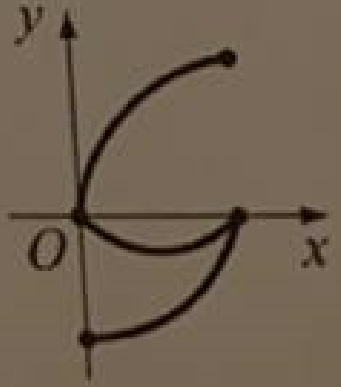
\includegraphics[scale=0.35]{graf930.png}}
\end{figure}\\
(А) $f(x)+g(x);$\\
(Б) $f(x)-g(x);$\\
(В) $f(x)\cdot g(x);$\\
(Г) $\cfrac{f(x)}{g(x)};$\\
(Д) $-f(x)\cdot g(x);$\\
81. Определите, при каких значениях параметра $a$ уравнение $(\sqrt{x}-2)(ax+2)(3x-2a)=0$ имеет ровно 2 различных корня.\\
82. а) Решите графически неравенство $\sqrt{x+3}>1+x;$\\
б) Сколько решений в зависимости от  $a$ имеет уравнение $\sqrt{x+3}=1+ax?$\\
83. Найдите все значения, которые принимает выражение $x+y,$ если $|y|=x(2-x).$\\
84. Найдите наименьшее значение суммы квадратов корней уравнения $x^2+3x+a=0$ и значение $a,$ при котором оно достигается.\\
85. Известно, что сумма квадратов корней уравнения $x^2-2x + q = 0$ равна 10084.
Найдите корни уравнения и значение $q.$\\
86. Известно, что сумма квадратов корней уравнения $x^2 -3x + q = 0$ равна 2249.
Найдите корни уравнения и $q.$\\
87. $f(x)=\sqrt{x^2+10x+34}+x-3.$ Найти координаты всех точек графика заданной функции,
равноудалённых от осей координат.\\
88. $f(x)=\sqrt{x^2+4x+8}-x-2.$ Найти координаты всех точек графика заданной функции,
равноудалённых от осей координат.\\
89. Прямая проходит через точку с координатами (10;0) и пересекает параболу $y=x^2$ в точках с абсциссами $x_1$ и $x_2.$ Найдите $\cfrac{1}{x_1}+\cfrac{1}{x_2}.$\\
90. Квадратный трёхчлен $f(x)=x^2+ax+b$ имеет два корня, один из которых лежит внутри отрезка  $[0;1],$ а
другой --- вне этого отрезка. Определите знак $f(b).$\\
91. Найдите целое число  $a,$ при котором выражение  $(x-a)(x-10)+1$ раскладывается в произведение $(x+b)(x+c)$ с целыми  $b$ и  $c.$\\
92. Известно, что $f(2x)=\cfrac{x+1}{2x+3}.$ Найдите корни уравнения $f(x)-1=0.$\\
93. При каком значении $a$ выражение $x^2+\cfrac{a^2}{x^2}-4\left(x+\cfrac{a}{x}\right)+10$ является полным квадратом?\\
94. При каких значениях параметра $a$ произведение корней уравнения $\cfrac{3x}{x^2+5x+9}=a$ равно 9?
\newpage
\section{Графики задачи}
1. Построить график функции $y=\cfrac{|x+1|}{x+1}(x-1).$\\
2. Построить график функции $y=\cfrac{|x-1|}{x-1}(x+1).$\\
3. Построить график функции $f(x)=\cfrac{|x^2-4x+3|}{|x-1|}.$\\
4. Построить график функции $f(x)=\cfrac{|x^2-x-2|}{|x+1|}.$\\
5. Построить график функции $f(x)=\cfrac{|x^2-4x|}{x}+|-x|.$\\
6. Построить график функции $f(x)=\cfrac{|x^2-2x|}{x-2}+|x|.$\\
7. Построить график функции $f(x)=2x^2-8x+q,$ если сумма квадратов корней этой функции равна 10.\\
8. Построить график функции $f(x)=-2x^2+2x+q,$ если квадрат разности корней этой функции равен 9.\\
9. Найти центр симметрии графика функции $y=\cfrac{x+1}{x}.$\\
10. Найти центр симметрии графика функции $y=\cfrac{1-x}{x}.$\\
11. Найти расстояние от начала координат до прямой $3y+4x=12.$\\
12. Найти расстояние от начала координат до прямой $3y-4x=12.$\\
13. Найдите оси симметрии графика функции $y=|x+1|+|x+3|.$\\
14. Найдите оси симметрии графика функции $y=|x-1|+|x-3|.$\\
15. Для окружности, заданной уравнением $x^2+y^2-4x-6y=0$ найдите центр и радиус.\\
16. Для окружности, заданной уравнением $x^2+y^2+6x-4y+2=0$ найдите центр и радиус.\\
17. Постройте график функции $y=\cfrac{|x-2|}{2-x}(x^2-2x).$\\
18. Постройте график функции $y=\cfrac{|x+2|}{2+x}(x^2+4x+3).$\\
19. Построить график $y=\cfrac{x^2+7x+6}{x+|x+2|}.$\\
20. Построить график $y=\cfrac{x^2-6x+5}{x-|x-2|}.$\\
21. Дано изображение графика функции $y=ax^2+bx+c$ (см. рис.). Определить знаки коэффициентов $a,\ b,\ c.$ Не забудьте обосновать ответ.
$$\begin{tikzpicture}[scale=1]
\begin{axis}[
    axis lines = middle,
    legend pos={south west},
    %xlabel = {$x$},
    %xlabel style={below right},
    %ylabel = {$y$},
    %title={$\text{Рис. 2}$},
    ymin=-3,
    ymax=3.8,
    xmin=-3,
    xmax=3.5,
    xtick=\empty,
	ytick=\empty,
    ]
	\addplot[domain=-1.4:3.4, samples=100, color=black] {0.2*(x^2-2*x-3)};
	%\addlegendentry{$\text{Рис. 1}$};
\end{axis}
\draw (2.75,5.7) node {\scriptsize $y$};
\draw (7,2.2) node {\scriptsize $x$};
\end{tikzpicture}$$
22. Дано изображение графика функции $y=ax^2+bx+c$ (см. рис.). Определить знаки коэффициентов $a,\ b,\ c.$ Не забудьте обосновать ответ.
$$\begin{tikzpicture}[scale=1]
\begin{axis}[
    axis lines = middle,
    legend pos={south west},
    %xlabel = {$x$},
    %xlabel style={below right},
    %ylabel = {$y$},
    %title={$\text{Рис. 2}$},
    ymin=-3,
    ymax=3.8,
    xmin=-3,
    xmax=3.5,
    xtick=\empty,
	ytick=\empty,
    ]
	\addplot[domain=-1.4:3.4, samples=100, color=black] {-0.2*(x^2-2*x+7)};
	%\addlegendentry{$\text{Рис. 1}$};
\end{axis}
\draw (2.75,5.7) node {\scriptsize $y$};
\draw (7,2.2) node {\scriptsize $x$};
\end{tikzpicture}$$
23. Построить график функции $y=\cfrac{\sqrt{(x+1)^2-4x}}{x^2-x}.$\\
24. Построить график функции $y=\cfrac{\sqrt{(x-1)^2+4x}}{x^2+x}.$\\
25. Изобразить множество точек на плоскости: $(|y|-3)(y+|x|-1)=0.$\\
26. Изобразить множество точек на плоскости: $(|x|-3)(x+|y|-1)=0.$\\
27. Пусть $f(x)=\cfrac{x-2+|2x-1|}{x^2-1}.$\\
а) постройте график функции $y=f(x);$\\
б) найдите область определения и множество значений функции;\\
в) сколько решений имеет уравнение $f(x)=a$ в зависимости от $a?$\\
28. Пусть $f(x)=\cfrac{x+2-|2x+1|}{x^2-1}.$\\
а) постройте график функции $y=f(x);$\\
б) найдите область определения и множество значений функции;\\
в) сколько решений имеет уравнение $f(x)=a$ в зависимости от $a?$\\
29. Изобразите на координатной плоскости множество точек, координаты которых удовлетворяют уравнению $\cfrac{x^2+y^2-9}{x^2-y^2}=0.$\\
30. Изобразите на координатной плоскости множество точек, координаты которых удовлетворяют уравнению $\cfrac{x^2+y^2-1}{x^2-y^2}=0.$\\
31. Построить график $y=\cfrac{x-2}{|x^2-2x|}.$\\
32. Построить график $y=\cfrac{3-x}{|x^2-3x|}.$\\
33. Найти расстояние от начала координат до прямой $y=1-\cfrac{x}{2}.$\\
34. Найти расстояние от начала координат до прямой $y=2-2x.$\\
35. Задайте формулой квадратичную функцию, если её график проходит через точки $A(0;-2)$ и $B(-2;4)$ и функция принимает значение $-4$ в единственной точке.\\
36. Задайте формулой квадратичную функцию, если её значения при $x=-1$ и при $x=2$ совпадают, её наибольшее значение равно 3, а график содержит точку $P(1;1).$\\
37. Пусть $f(x)=\cfrac{x-1+|x-1|}{x^2-1}.$\\
а) постройте график функции $y=f(x);$\\
б) найдите область определения и множество значений функции;\\
в) сколько решений имеет уравнение $f(x)=a$ в зависимости от $a?$\\
38. Пусть $f(x)=\cfrac{x+1-|x+1|}{x^2-1}.$\\
а) постройте график функции $y=f(x);$\\
б) найдите область определения и множество значений функции;\\
в) сколько решений имеет уравнение $f(x)=a$ в зависимости от $a?$\\
39. Изобразите на координатной плоскости множество точек, координаты которых удовлетворяют уравнению $\cfrac{x^2-y^2}{x^2+y^2-9}=0.$\\
40. Изобразите на координатной плоскости множество точек, координаты которых удовлетворяют уравнению $\cfrac{x^2-y^2}{x^2+y^2-1}=0.$\\
41. Изобразите на координатной плоскости множество точек, координаты которых удовлетворяют уравнению $\cfrac{x^2-y^2}{x^2+y^2-4}=0.$\\
42. Изобразите на координатной плоскости множество точек, координаты которых удовлетворяют уравнению $\cfrac{x^2-y^2}{x^2+y^2-16}=0.$\\
43. Дана функция $f(x)=|x^2-2x|.$\\
а) постройте график функции $y=f(x);$\\
б) сколько решений имеет уравнение $f(x)=a$ в зависимости от $a?$\\
44. Дана функция $f(x)=|x^2+2x|.$\\
а) постройте график функции $y=f(x);$\\
б) сколько решений имеет уравнение $f(x)=a$ в зависимости от $a?$\\
45. Изобразите на координатной плоскости множество точек, координаты которых удовлетворяют уравнению $\cfrac{yx-x^2-y+1}{x-1}=0.$\\
46. Изобразите на координатной плоскости множество точек, координаты которых удовлетворяют уравнению $\cfrac{(y-2x+1)(y+2x-1)}{y^2-x^2}=0.$\\
47. Прямая $a$ проходит через точки с координатами $(0;4)$ и $(6;0).$ Прямая $b$ проходит через точку с координатами $(0;8)$ и параллельна прямой $a.$ Найдите абсциссу точки пересечения прямой $b$ с осью $Ox.$\\
48. Прямая $a$ проходит через точки с координатами $(-6;0)$ и $(0;4).$ Прямая $b$ проходит через точку с координатами $(0;-6)$ и параллельна прямой $a.$ Найдите абсциссу точки пересечения прямой $b$ с осью $Ox.$\\
49. $\begin{tikzpicture}[scale=0.6]
\tikzset {line01/.style={line width =0.5pt}}
\tikzset{line02/.style={line width =1pt}}
\tikzset{line03/.style={dashed,line width =0.9pt}}
\filldraw [black] (0,0) circle (1pt);
\draw [->] (-2,0) -- (2,0);
\draw [->] (0,-3) -- (0,2);
\draw[line01] (-1.5,-1.7) -- (2,1);
\draw[line01] (-0.5,-2.7) -- (1,2);
\draw (1.25,2) node {\scriptsize $(1)$};
\draw (2,1.25) node {\scriptsize $(2)$};
\draw (2,0.25) node {\scriptsize $x$};
\draw (0.25,2) node {\scriptsize $y$};
\end{tikzpicture}$ На рисунке изображены две прямые с уравнениями (1) $y_1=k_1x+b_1$ и (2)
$y_2=k_2x+b_2.$ Расставьте в порядке возрастания числа $k_1,\ k_2,\ b_1,\ b_2.$\\
50. $\begin{tikzpicture}[scale=0.6]
\tikzset {line01/.style={line width =0.5pt}}
\tikzset{line02/.style={line width =1pt}}
\tikzset{line03/.style={dashed,line width =0.9pt}}
\filldraw [black] (0,0) circle (1pt);
\draw [->] (-2,0) -- (2,0);
\draw [->] (0,-2.8) -- (0,2);
\draw[line01] (-1.5,1.7) -- (2,-0.5);
\draw[line01] (-1,2.3) -- (1,-1.3);
\draw (1.25,-1.8) node {\scriptsize $(1)$};
\draw (2,-1.05) node {\scriptsize $(2)$};
\draw (2,0.25) node {\scriptsize $x$};
\draw (0.25,2) node {\scriptsize $y$};
\end{tikzpicture}$ На рисунке изображены две прямые с уравнениями (1) $y_1=k_1x+b_1$ и (2)
$y_2=k_2x+b_2.$ Расставьте в порядке возрастания числа $k_1,\ k_2,\ b_1,\ b_2.$\\
51. а) Постройте график функции $y=-|x^2-2x|.$\\
б) При каких $a$ прямая $y=a$ пересекает график функции в двух точках?\\
52. а) Постройте график функции $y=|x^2-4x|.$\\
б) При каких $a$ прямая $y=a$ пересекает график функции в двух точках?\\
53. Парабола задана уравнением $y=(x+a)^2+1.$ Прямая, задаваемая уравнением $y=4+2x$ имеет с параболой единственную общую точку. Найти $a.$\\
54. Парабола задана уравнением $y=-(x-a)^2+4.$ Прямая, задаваемая уравнением $y=2x-5$ имеет с параболой единственную общую точку. Найти $a.$\\
55. Изобразите множество точек, координаты которых удовлетворяют условию $|xy|>1.$\\
56. Изобразите множество точек, координаты которых удовлетворяют условию $|xy|<1.$\\
57. а) Постройте график функции $y=-\cfrac{4(x+2)}{x^2+x-2}.$\\
б) Найдите число решений уравнения $y=a$ в зависимости от $a.$\\
58. а) Постройте график функции $y=\cfrac{2(x-1)}{3x-2-x^2}.$\\
б) Найдите число решений уравнения $y=a$ в зависимости от $a.$\\
59. Докажите, что прямая $2x+6y-9=0$ не проходит через точки, обе координаты которых --- целые числа.\\
60. Докажите, что прямая $4x+6y-7=0$ не проходит через точки, обе координаты которых --- целые числа.\\
61. Постройте график функции $f(x)=x^2-|2x-2|-1$ и укажите её множество значений.\\
62. Постройте график функции $f(x)=(x+1)|x-1|$ и укажите промежутки её возрастания.\\
63. Постройте график функции $y=\cfrac{(x^2+2x-8)(x+2)}{|x+2|}.$ При каких $m$ прямая $y=m$ пересекает график функции в трёх точках?\\
64. Постройте график функции $y=\cfrac{(x^2-4x+3)(x-1)}{|x-1|}.$ При каких $m$ прямая $y=m$ пересекает график функции в трёх точках?\newpage
\noindent65. Могут ли параболы на рисунке  быть графиками функций  $f(x)=ax^2+b_1x+c$ и $g(x)=cx^2+b_2x+a?$
$$\begin{tikzpicture}[scale=1]
\begin{axis}[
    axis lines = middle,
    legend pos={south west},
    %xlabel = {$x$},
    %xlabel style={below right},
    %ylabel = {$y$},
    %title={$\text{Рис. 2}$},
    ymin=-3,
    ymax=3.8,
    xmin=-5.5,
    xmax=3.5,
    %xtick=\empty,
	%ytick=\empty,
    ]
	\addplot[domain=-5:1, samples=100, color=red] {-0.6*(x^2+4*x-1)};
	\addplot[domain=-5:1, samples=100, color=blue] {0.6*(x^2+4*x+2)};
%\addlegendentry{$\text{Рис. 1}$};
\end{axis}
\draw (3.75,5.7) node {\scriptsize $y$};
\draw (7,2.2) node {\scriptsize $x$};
\end{tikzpicture}$$
66. Могут ли параболы на рисунке  быть графиками функций  $f(x)=ax^2+b_1x+c$ и $g(x)=cx^2+b_2x+a?$
$$\begin{tikzpicture}[scale=1]
\begin{axis}[
    axis lines = middle,
    legend pos={south west},
    %xlabel = {$x$},
    %xlabel style={below right},
    %ylabel = {$y$},
    %title={$\text{Рис. 2}$},
    ymin=-5,
    ymax=3.8,
    xmin=-5.5,
    xmax=7.5,
    %xtick=\empty,
	%ytick=\empty,
    ]
	\addplot[domain=-3:7, samples=100, color=red] {-0.3*((x-4)^2+4*(x-4)-1)-2.5};
	\addplot[domain=-3:7, samples=100, color=blue] {0.3*((x-4)^2+4*(x-4)-5)};
%\addlegendentry{$\text{Рис. 1}$};
\end{axis}
\draw (2.75,5.7) node {\scriptsize $y$};
\draw (7,2.8) node {\scriptsize $x$};
\end{tikzpicture}$$
67. Постройте график функции $y=-\cfrac{4|x+2|}{x^2+2x}.$ При каком значении $m$ прямая $y=m$ имеет с графиком ровно одну общую точку?\\
68. Постройте график функции $y=-\cfrac{6|x-3|}{x^2-3x}.$ При каком значении $m$ прямая $y=m$ имеет с графиком ровно одну общую точку?\\
69. Постройте график функции $y=\cfrac{2x^2-8x}{|x-2|-2}$ и укажите те значения функции, которые она принимает ровно один раз.\\
70. Постройте график функции $y=\cfrac{3x^2-6x}{|x-1|-1}$ и укажите те значения функции, которые она принимает ровно один раз.\\
71. Может ли парабола, приведённая на рисунке (абсцисса её вершины равна 2), быть графиком функции $y=a(x-1)(x-4),$ где $a\neq0?$
$$\begin{tikzpicture}[scale=1]
\begin{axis}[
    axis lines = middle,
    legend pos={south west},
    %xlabel = {$x$},
    %xlabel style={below right},
    %ylabel = {$y$},
    %title={$\text{Рис. 2}$},
    ymin=-3,
    ymax=5.5,
    xmin=-1,
    xmax=6,
    %xtick=\empty,
	%ytick=\empty,
    ]
	\addplot[domain=-1:5, samples=100, color=black] {(2*x^2-8*x+5)};
	%\addplot[domain=-5:1, samples=100, color=blue] {0.6*(x^2+4*x+2)};
%\addlegendentry{$\text{Рис. 1}$};
\end{axis}
\draw (1.2,5.7) node {\scriptsize $y$};
\draw (7,2.2) node {\scriptsize $x$};
\end{tikzpicture}$$
72. Может ли парабола, приведённая на рисунке (абсцисса её вершины равна 3), быть графиком функции $y=a(x-2)(x-5),$ где $a\neq0?$
$$\begin{tikzpicture}[scale=1]
\begin{axis}[
    axis lines = middle,
    legend pos={south west},
    %xlabel = {$x$},
    %xlabel style={below right},
    %ylabel = {$y$},
    %title={$\text{Рис. 2}$},
    ymin=-3,
    ymax=5.5,
    xmin=-1,
    xmax=6,
    %xtick=\empty,
	%ytick=\empty,
    ]
	\addplot[domain=-1:6, samples=100, color=black] {(0.2*(3*x^2-18*x)+4)};
	%\addplot[domain=-5:1, samples=100, color=blue] {0.6*(x^2+4*x+2)};
%\addlegendentry{$\text{Рис. 1}$};
\end{axis}
\draw (1.2,5.7) node {\scriptsize $y$};
\draw (7,2.2) node {\scriptsize $x$};
\end{tikzpicture}$$
73. Постройте график функции $f(x)=-2x^{-2}$ при $x<0$ и $f(x)$ --- нечётная функция.\\
74. Постройте график функции $y=\cfrac{2x-3}{|x+2|}.$\\
75. Найдите все значения параметра $k,$ при которых гипербола $y=\cfrac{k}{x-2}$ пересекает прямую, задаваемую уравнением $y=x+1,$ в точке, лежащей на оси ординат.\\
76. Постройте график функции $y=\cfrac{x^3-x}{|x|}.$\\
77. Найдите все значения параметра $a,$ при которых прямая $y=a$ пересекает график функции $y=|x^2-4x|$ в двух точках.\\
78. Построить график функции $f(x)=\cfrac{|x^2-3x|(x+1)}{x}.$\\
79. Построить график функции $f(x)=\cfrac{|x^2+2x|(x-1)}{x}.$\\
80. Построить график функции $g(x)=\cfrac{2x+1}{2x^2+x}$ и определить:\\
а) при каких $k$ прямая $y=kx$ имеет одну общую точку с графиком функции $g(x)?$\\
б) при каких $b$ прямая $y=bx+2$ имеет одну общую точку с графиком функции $g(x)?$\\
81. Построить график функции $g(x)=\cfrac{x-2}{2x-x^2}$ и определить:\\
а) при каких $k$ прямая $y=kx$ имеет одну общую точку с графиком функции $g(x)?$\\
б) при каких $b$ прямая $y=bx+2$ имеет одну общую точку с графиком функции $g(x)?$\\
82. Пусть дана функция $f(x)=\cfrac{2-|x+3|}{x}.$\\
а) Постройте график функции $y=f(x),$\\
б) Решите неравенство $f(x)\geqslant-\cfrac{3}{2},$\\
в) Сколько корней имеет уравнение $f(x)=a$ в зависимости от $a?$\\
83. Пусть дана функция $f(x)=\cfrac{1-|x-2|}{x}.$\\
а) Постройте график функции $y=f(x),$\\
б) Решите неравенство $f(x)\leqslant\cfrac{3}{2},$\\
в) Сколько корней имеет уравнение $f(x)=a$ в зависимости от $a?$\\
84. Построить график функции $f(x)=\begin{cases} \sqrt{1-x},\ \text{ если } x\leqslant0,\\
x^2-|2x+1|,\ \text{ если } x>0.\end{cases}$\\
85. Пусть $f(x)=\begin{cases} 2, \text{ если } x>1,\\ -1, \text{ если } x<1,\\ 1, \text{ если } x=1.\end{cases}$\\
Постройте график $f(\sqrt{x-2}).$\\
86. Построить график функции $f(x)=\cfrac{1-|x-2|}{x}$ и решить неравенство $f(x)\leqslant 2.$\\
87. Построить график функции $f(x)=\cfrac{2-|x+3|}{x}$ и решить неравенство $f(x)\leqslant -2.$\\
88. Построить график функции $f(x)=|x^2-6x+5|$ и найти, при каком $k$ этот график имеет три общие точки с графиком функции $g(x)=k(x-7)+4.$\\
89. Построить график функции $f(x)=|x^2+2x-3|$ и найти, при каком $k$ этот график имеет три общие точки с графиком функции $g(x)=k(x+5)+4.$\\
90. а) Постройте график функции $f(x)=x^2-|2x-1|.$\\
б) При каких значениях параметра $a$ уравнение $x^2=|2x-1|+a$ имеет ровно два решения?\\
91. \begin{figure}[ht!]
\center{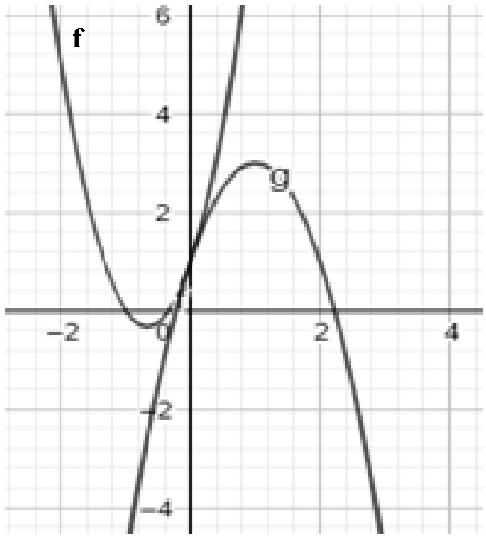
\includegraphics[scale=0.35]{grpar.png}}
\end{figure}\\
На рисунке параболы $f$ с уравнением $y=a_1 x^2+b_1x+c_1$ и $g$ с уравнением $y=a_2 x^2+b_2x+c_2$ касаются друг друга в точке, лежащей на оси ординат. Найдите соотношение между коэффициентами $a_1$ и $a_2;\ b_1$ и $b_2;\ c_1$ и $c_2.$\\
92. Постройте график функции $f(x)=\cfrac{x^2+x}{x}\cdot\sqrt{x^2-6x+9}.$\\
93. Постройте график функции $f(x)=\cfrac{x^2+x-6}{2-x}\cdot\sqrt{x^2-2x+1}.$\\
94. Известно, что графики функций $y=x^2+p$ и $y=-4x-5$ имеют ровно одну общую точку. Определите координаты этой точки. Постройте графики заданных функций в одной системе координат.\\
95. Изобразите на координатной плоскости множество точек, координаты которых удовлетворяют условию\\
(А) $|2x-y|=x;$\\
(Б) $|2x-y|<x.$\\
96. $f(x)=\begin{cases} \cfrac{3x-1}{x+1},\ x\neq-1\\a+2,\ x=-1 \end{cases}$\\
а) Построить график функции при $a=3.$\\
б) При каких $a$ уравнение $f(x)=a-1$ не имеет решений?\\
в) При каких $a$ прямая $y=ax+1$ имеет с графиком функции $f(x)$ три общие точки?\\
97. $f(x)=\begin{cases} \cfrac{3x+1}{x-1},\ x\neq1\\3-a,\ x=1 \end{cases}$\\
а) Построить график функции при $a=-1.$\\
б) При каких $a$ уравнение $f(x)=a+1$ не имеет решений?\\
в) При каких $a>0$ прямая $y=ax+2$ имеет с графиком функции $f(x)$ три общие точки?\\
98. $f(x)=\begin{cases} 4-|x+1|,\ x<2\\ x^2-6x+4,\ x\geqslant 2\end{cases}$\\
а) Построить график функции $f(x)$\\
б) При каких $a$ уравнение $f(x)=2a$ имеет два решения?\\
99. $f(x)=\begin{cases} |x-3|-4,\ x>1\\ -x^2-3x+4,\ x\leqslant 1\end{cases}$\\
а) Построить график функции $f(x)$\\
б) При каких $a$ уравнение $f(x)=\cfrac{a}{2}$ имеет два решения?\\
100. Постройте график функции $y=f(x),$ где $f(x)=\begin{cases}\cfrac{4}{x}, \text{ при } x<-2,\\
\cfrac{x}{2}-1, \text{ при } -2\leqslant x \leqslant 2,\\
x^2-6x+8, \text{ при } x>2.\end{cases}$\\
При каких значениях $m$ прямая $y = m$ имеет с графиком этой функции две общие точки?\\
101. Постройте график функции $y=f(x),$ где $f(x)=\begin{cases}-\cfrac{1}{x}, \text{ при } x\leqslant -1,\\
-x, \text{ при } -1< x \leqslant 1,\\
-x^2+4x-4, \text{ при } x>1.\end{cases}$\\
При каких значениях $m$ прямая $y = m$ имеет с графиком этой функции три общие точки?
\newpage
\section{Прогрессии задачи}
1. Туристы поднимаются на перевал высотой 4800 м. В первый день они поднялись на высоту 1800 метров, а в каждый последующий день набирали высоты на 200 м меньше, чем в предыдущий. Через сколько дней туристы достигнут перевала?\\
2. Сплавляясь по реке в первый день, геологи проплыли 40 км, а в каждый последующий день проплывали на 5 км меньше, чем в предыдущий. Сколько дней сплавлялись геологи, если длина реки равна 130 км?\\
3. Найти сумму всех натуральных чисел, не превосходящих 165, которые при делении на 7 дают в остатке 5.\\
4. Найти сумму всех натуральных чисел, не превосходящих 300, которые при делении на 11 дают в остатке 3.\\
5. Найти сумму всех трёхзначных чисел, не кратных 5.\\
6. Найти сумму всех двузначных чисел, не кратных 3.\\
7. В геометрической прогрессии с положительными числами $b_3=32;\ b_7=2.$ Найти $b_5.$\\
8. В геометрической прогрессии с положительными числами $b_2=16;\ b_{10}=4.$ Найти $b_6.$\\
9. При каких $a$ числа $a^2;\ 4a;\ 2a+5$ являются тремя последовательными членами арифметической прогрессии?\\
10. При каких $a$ числа $a^2;\ 3a;\ a+4$ являются тремя последовательными членами арифметической прогрессии?\\
11. Третий член арифметической прогрессии равен 10, а восьмой равен 30. Сколько членов прогрессии нужно взять, чтобы их сумма равнялась 242?\\
12. Третий член арифметической прогрессии равен 21, а девятый равен 51. Сколько членов прогрессии нужно взять, чтобы их сумма равнялась 396?\\
13. Найдите сумму всех трёхзначных чисел, не делящихся на 7 и имеющих последней цифру 3.\\
14. Найдите сумму всех трёхзначных чисел, не делящихся на 11 и имеющих последней цифру 5.\\
15. Найдите сумму первых восьми членов геометрической прогрессии, второй член который равен 6, а четвёртый 24.\\
16. Найдите сумму первых шести членов геометрической прогрессии, третий член который равен 54, а пятый 6.\\
17. Сумма седьмого и тринадцатого членов арифметической прогрессии равна 16. Найдите её десятый член.\\
18. Сумма пятого и семнадцатого членов арифметической прогрессии равна 20. Найдите её одиннадцатый член.\\
19. Найдите сумму первых шести членов арифметической прогрессии, шестой член которой равен $\cfrac{3}{4},$ а десятый $\cfrac{7}{4}.$\\
20. Найдите сумму первых десяти членов арифметической прогрессии, третий член которой равен $(-1),$ а пятый $3.$\\
21. Найдите сумму первых шести членов арифметической прогрессии, первый член которой равен $1,2,$ а четвёртый $1,8.$\\
22. Найдите сумму первых десяти членов арифметической прогрессии, второй член которой равен $(-5),$ а разность шестого и четвёртого $6.$\\
23. Бригада маляров красит забор длиной 240 м, ежедневно увеличивая норму покраски на одно и то же число метров. Известно, что за первый и последний день в сумме бригада покрасила 60 м забора. Определите, сколько дней бригада красила весь забор.\\
24. Улитка ползёт от одного дерева до другого. Каждый день она проползает на одно и то же расстояние больше, чем в предыдущий день. Известно, что за первый и последний день улитка проползла в общей сложности 10 метров. Определите, сколько дней улитка потратила на весь путь, если расстояние между деревьями 150 метров.\\
25. Три числа составляют геометрическую прогрессию. Если первые два из них оставить без изменений, а из последнего вычесть первое, то полученные три числа составят арифметическую прогрессию. Найдите разность арифметической прогрессии, если второе из взятых чисел равно 6.\\
26. Три числа составляют арифметическую прогрессию. Если первые два числа оставить без изменения, а к третьему прибавить сумму двух первых, то полученные числа составят геометрическую прогрессию. Найдите знаменатель этой геометрической прогрессии.\\
27. Сумма первых десяти членов арифметической прогрессии равна 30; четвёртый, седьмой и пятый члены этой прогрессии в указанном порядке составляют геометрическую прогрессию. Найдите разность арифметической прогрессии, если известно, что все её члены различны.\\
28. Сумма первых тринадцати членов арифметической прогрессии равна 130; четвёртый, десятый и седьмой члены этой прогрессии в указанном порядке составляют геометрическую прогрессию. Найдите разность арифметической прогрессии, если известно, что все её члены различны.\\
29. Последовательность $(a_n)$ --- арифметическая прогрессия. Известно, что: $a_5+a_9=40.$ Найдите $a_3+a_7+a_{11}.$\\
30. Последовательность $(a_n)$ --- арифметическая прогрессия. Известно, что: $a_4+a_6=38.$ Найдите $a_2+a_5+a_{8}.$\\
31. Числа $a_1,\ a_2,\ldots,a_{21}$ образуют арифметическую прогрессию. Известно, что сумма членов этой прогрессии с нечётными номерами на 15 больше суммы членов с чётными номерами. Найдите $a_{12},$ если $a_{20}=3a_9.$\\
32. Числа $a_1,\ a_2,\ldots,a_{19}$ образуют арифметическую прогрессию. Известно, что удвоенная сумма членов этой прогрессии с чётными номерами на 10 больше суммы всех членов. Найдите $a_{13},$ если $a_{3}=2a_4.$\\
33. Второй член арифметической прогрессии составляет $88\%$ от первого. Найдите сколько процентов первый член составляет от пятого.\\
34. Сумма первых трёх членов убывающей $(|q|<1)$ геометрической прогрессии равна 21, а сумма их квадратов --- 189. Найдите первый член и знаменатель данной прогрессии.\\
35. Могут ли длины сторон прямоугольного треугольника образовывать геометрическую прогрессию?\\
36. Найдите сумму всех трёхзначных чисел, не делящихся на 11.\\
37. Найдите сумму всех трёхзначных чисел, кратных 7, но не кратных 5.\\
38. Найдите сумму всех трёхзначных чисел, кратных 5, но не кратных 7.\\
39. Найти сумму всех чётных двузначных чисел, делящихся на 3.\\
40. Найти сумму всех двузначных чисел, делящихся на 7.\\
41. В арифметической прогрессии $(a_n)$ $a_1=4.$ При каком значении разности прогрессии произведение $a_5$ и $a_7$ будет наименьшим?\\
42. Найти сумму всех трёхзначных чисел, которые при делении на 11 дают остаток 5.\\
43. Найти сумму всех трёхзначных чисел, которые при делении на 13 дают остаток 7.\\
44. Различные числа $a,\ b,\ c$ являются последовательными членами некоторой геометрической прогрессии. Эти же числа в том же порядке можно рассматривать как первый, второй и четвёртый члены некоторой арифметической прогрессии. Найдите эти числа, если их сумма равна 35.\\
45. Различные числа $a,\ b,\ c$ являются соответственно первым, вторым и шестым членами некоторой арифметической прогрессии. Эти же числа в том же порядке являются последовательными членами некоторой геометрической прогрессии. Найдите эти числа, если $a+c-b=13.$\\
46. Числа $a_1,\ a_2,\ldots$ образуют арифметическую прогрессию. Известно, что $a_{17}+a_{23}=400,\ a_{20}+a_{108}=224.$ Найдите $a_{1}+a_2+\ldots+a_{239}.$\\
47. Произведение седьмого и восьмого членов непостоянной арифметической прогрессии равно произведению пятого и девятого её членов. Найдите одиннадцатый член данной прогрессии.\\
48. Цифры трёхзначного числа образуют арифметическую прогрессию. Если из этого числа вычесть 792, то получится число, записанное теми же цифрами, но в обратном порядке. Если же из цифры десятков вычесть 2, а остальные цифры оставить без изменения, то получится число, цифры которого образуют геометрическую прогрессию. Найдите исходное число.\\
49. Цифры трёхзначного числа образуют геометрическую прогрессию. Если из этого числа вычесть 792, то получится число, записанное теми же цифрами, но в обратном порядке. Если же из цифры сотен вычесть 4, а остальные цифры оставить без изменения, то получится число, цифры которого образуют арифметическую прогрессию. Найдите исходное число.
\newpage
\section{Тригонометрия задачи}
1. Упростить $\cfrac{\cos(3\alpha)+\cos(4\alpha)+\cos(5\alpha)}{\sin(3\alpha)+\sin(4\alpha)+\sin(5\alpha)}.$\\
2. Упростить $\cfrac{\cos(6\alpha)+\cos(8\alpha)+\cos(10\alpha)}{\sin(6\alpha)+\sin(8\alpha)+\sin(10\alpha)}.$\\
3. Найти $\cos(\alpha),$ если $\sin\left(\alpha+\cfrac{\pi}{4}\right)=-\cfrac{12}{13},$ а угол $\alpha-\cfrac{\pi}{4}$ находится в $III$ четверти.\\
4. Найти $\sin(\alpha),$ если $\cos\left(\alpha-\cfrac{3\pi}{4}\right)=\cfrac{5}{13},$ а угол $\alpha-\cfrac{\pi}{4}$ находится в $II$ четверти.\\
5. Пусть $tg(2\alpha)=\cfrac{1}{\sqrt{3}}.$ Найти все значения, которые может принимать $\sin(\alpha)+\cos(\alpha).$\\
6. Пусть $ctg(2\alpha)=\sqrt{3}.$ Найти все значения, которые может принимать $\sin(\alpha)-\cos(\alpha).$\\
7. Построить график функции $f(x)=-\sqrt{\sin^2\left(\cfrac{x}{2}\right)}+\cfrac{\cos\left(\cfrac{x}{2}\right)-\cos\left(\cfrac{3x}{2}\right)}
{\sqrt{2-2\cos(2x)}}.$\\
8.\ Построить график функции $f(x)=\cfrac{\cos\left(\cfrac{3x}{2}\right)-\cos\left(\cfrac{x}{2}\right)}
{\sqrt{\cos^2(x)+\sin^2(x)-2\cos(2x)+1}}+\left|\sin\left(\cfrac{x}{2}\right)\right|.$\\
9. Упростить: $\cfrac{1-\cos(2\alpha)+\sin(2\alpha)}{1+\cos(2\alpha)+\sin(2\alpha)}.$\\
10. Упростить: $\cfrac{1+\cos(\alpha)+\cos(2\alpha)+\cos(3\alpha)}{\cos(\alpha)+\cos(2\alpha)}.$\\
11. Вычислить: $tg(41^\circ)\cdot tg(42^\circ)\cdot \ldots \cdot tg(48^\circ)\cdot tg(49^\circ).$\\
12. Вычислить: $ctg(41^\circ)\cdot ctg(42^\circ)\cdot \ldots \cdot ctg(48^\circ)\cdot ctg(49^\circ).$\\
13. Упростить: $\cfrac{\sin(\alpha)}{1+\cos(\alpha)}+ctg(\alpha).$\\
14. Упростить: $\cfrac{\cos(\alpha)}{1+\sin(\alpha)}+tg(\alpha).$\\
15. Вычислите: $ctg(160^\circ)\cdot tg(20^\circ)\cdot ctg(135^\circ).$\\
16. Вычислите: $ctg(140^\circ)\cdot tg(40^\circ)\cdot tg(135^\circ).$\\
17. Найдите $tg(\alpha),$ если $\cos(\alpha)=-\cfrac{5}{13},\ 90^\circ<\alpha<180^\circ.$\\
18. Найдите $ctg(\alpha),$ если $\sin(\alpha)=\cfrac{5}{13},\ 90^\circ<\alpha<180^\circ.$\\
19. Вычислите $\cos(\alpha),$ если $\sin\left(\alpha+\cfrac{\pi}{6}\right)=-\cfrac{13}{14},$ а $\left(\alpha-\cfrac{\pi}{3}\right)$ --- угол $III$ четверти.\\
20. Вычислите $\sin(\alpha),$ если $\cos\left(\alpha-\cfrac{3\pi}{4}\right)=\cfrac{5}{13},$ а $\left(\alpha-\cfrac{\pi}{4}\right)$ --- угол $I$ четверти.\\
21. Дано: $\sin(\alpha)=0,28,\ \cfrac{\pi}{2}<\alpha<\pi.$ Найдите $\sin(2\alpha).$\\
22. Дано: $\cos(\alpha)=\cfrac{5}{13},\ -\cfrac{\pi}{2}<\alpha<0.$ Найдите $\sin(2\alpha).$\\
23. Дано: $\sin(\alpha)=-0,28,\ \pi<\alpha<\cfrac{3\pi}{2}.$ Найдите $\sin(2\alpha).$\\
24. Дано: $\cos(\alpha)=-\cfrac{5}{13},\ \pi<\alpha<\cfrac{3\pi}{2}.$ Найдите $\sin(2\alpha).$\\
25. Дано: $\sin(\alpha)=\cfrac{12}{13},\ \cfrac{\pi}{2}<\alpha<\pi.$ Найдите $\cos(2\alpha).$\\
26. Дано: $\cos(\alpha)=-\cfrac{5}{13},\ \cfrac{\pi}{2}<\alpha<\pi.$ Найдите $\sin(2\alpha).$\\
27. В треугольнике $ABC$ угол $C$ равен $90^\circ,\ \sin(A)=\cfrac{7}{25}.$ Найдите $\cos(A).$\\
28. В треугольнике $ABC$ угол $C$ равен $90^\circ,\ \sin(A)=\cfrac{24}{25}.$ Найдите $\sin(B).$\\
29. Вычислите $\sin(2\alpha),$ если $tg(\alpha)=3.$\\
30. Вычислите $\cos(2\alpha),$ если $ctg(\alpha)=0,5.$\\
31. Найти $\cfrac{\sin(\alpha)+2\cos(\alpha)}{\sin(\alpha)-\cos(\alpha)},$ если $tg(\alpha)=\cfrac{5}{4}.$
\newpage
\section{Стандартные задачи}
1. Найдите число $N,$ если 6 составляет $40\%$ от $N+5.$\\
2. Найдите число $N,$ если 9 составляет $75\%$ от $N+3.$\\
3. При каких натуральных $n$ значение данного выражения является целым числом: $\cfrac{2n^2+5n-5}{n+1}?$\\
4. При каких натуральных $n$ значение данного выражения является целым числом: $\cfrac{3n^2+4n-3}{n+3}?$\\
5. Сплавлено 40 г золота одной пробы и 60 г золота другой пробы и получено золото 62-й пробы. Какой пробы было золото первого и второго слитков, если при сплаве их поровну получается золото 61-й пробы?\\
6. Имеется сталь двух сортов с содержанием никеля в $5\%$ и $40\%.$ Сколько нужно взять каждого из этих сортов стали, чтобы получить 140 т стали с содержанием никеля в $30\%?$\\
7. Бассейн заполняется водой, поступающей через две трубы. Одна труба может заполнить бассейн за 12 часов, а другая --- за 20 часов. За сколько часов заполнится бассейн двумя трубами, работающими одновременно?\\
8. Вода, поступающая в первую трубу, может наполнить бассейн за 6 часов, а вода, вытекающая из второй трубы, может опорожнить его за 15 часов. За сколько часов наполнится бассейн, если обе трубы будут одновременно открыты?\\
9. Из А и В выехали два автомобиля. Первый проехал с постоянной скоростью весь путь. Второй проехал первую половину пути со скоростью, меньшей скорости первого на 13 км/ч, а вторую половину пути --- со скоростью 78 км/ч, в результате чего прибыл в В одновременно с первым автомобилем. Найдите скорость первого автомобиля, если известно, что она больше 48 км/ч. Ответ дайте в км/ч.\\
10. Из А и В выехали два автомобиля. Первый проехал с постоянной скоростью весь путь. Второй проехал первую половину пути со скоростью, меньшей скорости первого на 16 км/ч, а вторую половину пути --- со скоростью 96 км/ч, в результате чего прибыл в В одновременно с первым автомобилем. Найдите скорость первого автомобиля, если известно, что она больше 57 км/ч. Ответ дайте в км/ч.\\
11. Два печника, работая вместе, могут сложить печь за 12 часов. Если сначала один первый печник будет работать 2 часа, а затем один второй --- 3 часа, то они выполнят только $20\%$ всей работы. За сколько часов может сложить печь один первый печник?\\
12. Две бригады, работая вместе, могут закончить уборку урожая за 8 дней. Если сначала первая бригада будет работать 3 дня, а затем одна вторая --- 12 дней, то они выполнят $75\%$ всей работы. За сколько дней может закончить уборку урожая одна вторая бригада?\\
13. Велосипедист выехал с постоянной скоростью из города А в город В, расстояние между которыми равно 70 км. На следующий день он отправился обратно в А со скоростью на 3 км/ч больше прежней. По дороге он сделал остановку на 3 часа. В результате он затратил на обратный путь столько же времени, сколько на путь из А в В. Найдите скорость велосипедиста на пути из В в А. Ответ дайте в км/ч.\\
14. Велосипедист выехал с постоянной скоростью из города А в город В, расстояние между которыми равно 98 км. На следующий день он отправился обратно в А со скоростью на 7 км/ч больше прежней. По дороге он сделал остановку на 7 часов. В результате он затратил на обратный путь столько же времени, сколько на путь из А в В. Найдите скорость велосипедиста на пути из В в А. Ответ дайте в км/ч.\\
15. Имеется 10 литров 60-процентного раствора соли. Сколько литров воды надо долить, чтобы получить 40-процентный раствор соли?\\
16. В сосуд, содержащий 5 литров 12-процентного водного раствора некоторого вещества, добавили 7 литров воды. Сколько процентов составляет концентрация получившегося раствора?\\
17. Половину времени, затраченного на дорогу, автомобиль ехал со скоростью 90 км/ч, а вторую половину времени --- со скоростью 60 км/ч. Найдите среднюю скорость автомобиля на протяжении всего пути.\\
18. Первую половину пути автомобиль проехал со скоростью 90 км/ч, вторую половину пути --- со скоростью 60 км/ч. Найдите среднюю скорость автомобиля на протяжении всего пути.\\
19. Игорь и Паша могут покрасить забор за 3 часа. Паша и Володя могут покрасить этот же забор за 6 часов, Володя и Игорь --- за 4 часа. За какое время мальчики покрасят забор, работая вместе?\\
20. Маша и Настя могут вымыть окно за 20 минут. Настя и Лена могут вымыть это же окно за 15 минут, а Маша и Лена --- за 12 минут. За какое время девочки вымоют окно, работая втроём?\\
21. Мальчик сбежал вниз по движущемуся эскалатору и насчитал 20 ступенек. Затем он пробежал вверх по тому же эскалатору с той же скоростью относительно эскалатора и насчитал 60 ступенек. Сколько ступенек он насчитал бы, спустившись по неподвижному эскалатору?\\
22. Мальчик сбежал вниз по движущемуся эскалатору и насчитал 30 ступенек. Затем он пробежал вверх по тому же эскалатору с той же скоростью относительно эскалатора и насчитал 70 ступенек. Сколько ступенек он насчитал бы, спустившись по неподвижному эскалатору?\\
23. Из трёхзначного числа вычли сумму его цифр. Может ли разность быть равной 189?\\
24. Из трёхзначного числа вычли сумму его цифр. Может ли разность быть равной 180?\\
25. При каких натуральных $n$ значение выражения $\cfrac{n^2+5n-8}{n+3}$ является целым числом?\\
26. При каких натуральных $n$ значение выражения $\cfrac{-n^2+2n-31}{n+3}$ является целым числом?\\
27. Заказ на 180 деталей первый рабочий выполняет на 3 часа быстрее, чем второй. Сколько деталей в час делает второй рабочий, если известно, что первый в час делает на 3 детали больше?\\
28. Заказ на 156 деталей первый рабочий выполняет на 1 час быстрее, чем второй. Сколько деталей в час делает второй рабочий, если известно, что первый в час делает на 1 деталь больше?\\
29. В январе товар стоил 30000 рублей. В марте цену на товар подняли на $4\%,$ а в июле снизили на $4\%.$ Сколько стоил товар в июле?\\
30. В феврале товар стоил 20000 рублей. В мае цену подняли на $6\%,$ а в августе снизили
на $6\%.$ Сколько стоил товар в августе?\\
31. Расстояние между пристанями А и В равно 18 км. Из А в В по течению реки отправился плот, а через 30 мин за ним отправилась моторная лодка, которая, прибыв в пункт В, тотчас повернула обратно и возвратилась в пункт А. К этому времени плот прошёл 9 км. Найдите скорость лодки в неподвижной воде, если скорость течения реки равна 50 м/мин.\\
32. Расстояние между пристанями А и В равно 14 км. Из А в В по течению реки отправился плот, а через 44 мин за ним отправилась моторная лодка, которая, прибыв в пункт В, тотчас повернула обратно и возвратилась в пункт А. К этому времени плот прошёл 7 км. Найдите скорость лодки в неподвижной воде, если скорость течения реки равна 50 м/мин.\\
33. Один раствор содержит $20\%$ (по объёму) соляной кислоты, а второй содержит $70\%$ кислоты. Сколько литров первого и второго растворов нужно взять, чтобы получить 100 л $50\%$-го раствора соляной кислоты?\\
34. Имеется кусок сплава меди с оловом массой 15 кг, содержащий $40\%$ меди. Сколько чистого олова надо прибавить к этому куску, чтобы получившийся новый сплав содержал $30\%$ меди?\\
35. В каждом из двух ящиков лежит 15 шаров. Число синих шаров в обоих ящиках равно 8, остальные шары --- красные. Сколько красных шаров лежит в каждом ящике, если в первом ящике на каждый синий шар приходится в 2 раза меньше красных шаров, чем во втором?\\
36. В каждом из двух ящиков лежит 40 кубиков. Число жёлтых кубиков в обоих ящиках равно 14, остальные кубики --- зелёные. Сколько зелёных кубиков лежит в каждом ящике, если в первом ящике на каждый жёлтый кубик приходится в 3 раза меньше зелёных кубиков, чем во втором?\\
37. На финальной распродаже скидка на все товары составляет $50\%,$ при этом по карте магазина постоянным покупателям предоставляется дополнительная скидка $30\%.$ При каком последовательном использовании скидок итоговая скидка больше и сколько она составит в каждом случае?\\
38. На финальной распродаже скидка на все товары составляет $70\%,$ при этом по карте магазина постоянным покупателям предоставляется дополнительная скидка $20\%.$ При каком последовательном использовании скидок итоговая скидка больше и сколько она составит в каждом случае?\\
39. Перед отправкой тепловоз издал гудок с частотой $f_0=593$ Гц. Чуть позже издал гудок подъезжающий к платформе тепловоз. Из-за эффекта Допплера частота второго гудка $f$ больше первого: она зависит от скорости тепловоза по закону $f(v)=\cfrac{f_0}{1-\frac{v}{c}}$ (Гц), где $c$ --- скорость звука в м/с. Человек, стоящий на платформе, различает сигналы по тону, если они отличаются не менее, чем на 7 Гц. Определите, с какой минимальной скоростью приближался к платформе тепловоз, если человек смог различить сигналы, а $c=300$ м/с. Ответ выразите в м/с.\\
40. Перед отправкой тепловоз издал гудок с частотой $f_0=154$ Гц. Чуть позже издал гудок подъезжающий к платформе тепловоз. Из-за эффекта Допплера частота второго гудка $f$ больше первого: она зависит от скорости тепловоза по закону $f(v)=\cfrac{f_0}{1-\frac{v}{c}}$ (Гц), где $c$ --- скорость звука в м/с. Человек, стоящий на платформе, различает сигналы по тону, если они отличаются не менее, чем на 6 Гц. Определите, с какой минимальной скоростью приближался к платформе тепловоз, если человек смог различить сигналы, а $c=320$ м/с. Ответ выразите в м/с.\\
41. Из Вены в Стамбул отправился пассажирский поезд, а навстречу ему из Стамбула в Вену через 3 часа вышел товарный поезд. После встречи пассажирский поезд ехал еще 3 часа до Стамбула, а товарный ---
6 часов до Вены. Сколько часов был в пути каждый из поездов?\\
42. Из пункта А в пункт Б отправился велосипедист Вася, а через 2 минуты ему навстречу из Б в А выехал велосипедист Петя. От места встречи на дороге Вася добрался до пункта Б за 11 минут, а Петя до пункта А за 9 минут. Сколько минут был в пути каждый из них?\\
43. К краю большого квадратного листа приложили маленький квадратик, как показано на рисунке, и в результате периметр листа увеличился на $5\%.$ На сколько $\%$ увеличилась площадь листа?
\begin{figure}[h]
\center{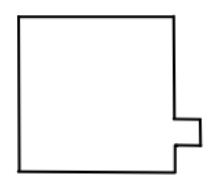
\includegraphics[scale=0.35]{2q2.png}}
\end{figure}\\
44. От края большого квадратного листа отрезали маленький квадратик, как показано на рисунке, и в результате периметр листа увеличился на $10\%.$ На сколько $\%$ уменьшилась площадь листа?
\begin{figure}[h]
\center{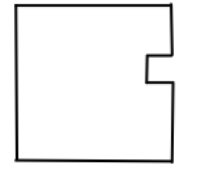
\includegraphics[scale=0.35]{1q1.png}}
\end{figure}\\
45. Из бутыли, наполненной $12\%$-ным раствором соли, отлили 1 л и долили бутыль водой, затем отлили ещё литр и опять долили водой. В бутыли оказался $3\%$-ный раствор соли. Какова вместимость бутыли?\\
46. Фляга наполнена $96\%$-ным раствором соляной кислоты. Из неё отлили 12 л кислоты и дополнили флягу водой. Затем из фляги отлили ещё 18 л и снова дополнили её водой, после чего концентрация кислоты во фляге составила $32\%.$ Найдите объём фляги.\\
47. В трёх литрах воды размешали пять чайных ложек минерального удобрения, а в десяти литрах --- две. Оба раствора слили в один бак и получили раствор удобрения нужной концентрации. Сколько чайных ложек удобрения нужно размешать в 65 литрах воды для получения раствора удобрения такой же концентрации?\\
48. Банк в конце года начисляет $20\%$ к сумме, находящейся на счёте в начале года. Каким станет вклад 50000 рублей через 3 года?\\
49. Банк в конце года начисляет $10\%$ к сумме, находящейся на счёте в начале года. Каким станет вклад 70000 рублей через 3 года?\\
50. Два велосипедиста выехали одновременно из пункта $A$ в $B,$ первый со скоростью 24 км/ч, а второй --- 18 км/ч. Спустя час вслед за ними выехал автомобиль, который обогнал второго велосипедиста на 10 минут раньше, чем первого. Найдите скорость автомобиля.\\
51. Две лодки вышли одновременно из пункта $A$ в $B,$ первая со скоростью 12 км/ч, а вторая --- 9 км/ч. Спустя час вслед за ними вышел катер, который обогнал вторую лодку на 10 минут раньше, чем первую. Найдите скорость катера.\\
52. В предвыборном штабе депутат листовки печатают 4 станка разной мощности. При печатании листовок на 1-м, 2-м и 4-м станках весь тираж будет готов за 1 час 48 мин; при печатании на 1-м, 2-м и 3-м --- за 2 часа 15 минут, а если листовки печатать на 3-м и 4-м станках, то тираж напечатают за 1,5 часа. За какое время будет готов весь тираж при совместной работе всех четырёх станков?\\
53. Автобус выехал из пункта $A$ в пункт $B.$ Не доехав 15 км до середины пути, автобус остановился для ремонта, которые занял 1 ч 30 мин. Оставшуюся часть пути автобус шёл со скоростью, на 20 км/ч больше первоначальной, и поэтому приехал в пункт $B$ вовремя. Если бы автобус весь путь шёл со скоростью, на 9 км/ч большей первоначальной, то он затратил бы на весь путь 10 ч. Найдите первоначальную скорость автобуса и расстояние между пунктами $A$ и $B.$\\
54. Автобус выехал из пункта $C$ в пункт $D.$ Проехав половину пути и ещё 40 км с постоянной скоростью, автобус остановился для ремонта, который занял 50 мин.  Оставшуюся часть пути автобус шёл со скоростью, на 5 км/ч меньшей первоначальной, и поэтому приехал в пункт $D$ с опозданием на 1 ч. Если бы автобус весь путь шёл со скоростью, на 20 км/ч меньшей первоначальной, то она затратил бы на весь путь 8 ч. Найдите первоначальную скорость автобуса и расстояние между пунктами $C$ и $D.$\\
55. Имеется два сосуда с водным раствором серной кислоты. В первом сосуде содержится 70 мл чистой кислоты, а во втором --- 60 мл. Слив содержимое этих сосудов вместе, получили 600 мл нового раствора. Найдите концентрацию кислоты в каждом из первоначальных растворов, если концентрация во втором сосуде была на $20\%$ меньше, чем в первом.\\
56. На предприятии доля сотрудников с высшим образованием составляла $80\%.$ После того как на работу было принято 30 новых специалистов с высшим образованием, доля сотрудников с высшим образованием увеличилась до $85\%.$ Сколько сотрудников теперь работает на предприятии?\\
57. Доля брака в партии изделий составляла $9\%.$ На стадии контроля качества удалось выявить и изъять из партии 40 бракованных изделий. Сколько изделий осталось в партии, если доля брака в ней составляет теперь $2,5\%?$\\
58. Два поезда выезжают одновременно из пунктов А и В навстречу друг другу. После их встречи первый прибывает в пункт В через 50 часов, а второй --- в пункт А через 8 часов. Сколько времени прошло от начала движения поездов до их встречи, если они двигались с постоянными скоростями?\\
59. Два велосипедиста выезжают одновременно из пунктов А и В навстречу друг другу. После их встречи первый прибывает в пункт В через 48 минут, а второй --- в пункт А через 27 минут. Сколько времени прошло от начала движения велосипедистов до их встречи, если велосипедисты двигались с постоянными скоростями?
\newpage
\section{Нестандартные задачи}
1. {\it Логарифмом} числа $a>0$ по основанию 2 называется показатель степени, в которую нужно возвести 2, чтобы получить $a.$ Обозначение: $\log_2 a.$\\
Вычислить: а)$\log_2 8;$ б)$2^{\log_2 3};$ в) $4^{\log_2 5};$ г) Подумайте о том, что означает символ $\log_5 a$ и вычислите $2^{\log_5 3\cdot\log_25}.$\\
2. {\it Логарифмом} числа $a>0$ по основанию 3 называется показатель степени, в которую нужно возвести 3, чтобы получить $a.$ Обозначение: $\log_3 a.$\\
Вычислить: а)$\log_3 27;$ б)$3^{\log_3 2};$ в) $9^{\log_3 7};$ г) Подумайте о том, что означает символ $\log_5 a$ и вычислите $3^{\log_5 3\cdot\log_3 5}.$\\
3. Тринадцать различных натуральных чисел в сумме дают 92. Найдите эти числа.\\
4. Одиннадцать различных натуральных чисел в сумме дают 67. Найдите эти числа.\\
5. Три ученика Саша, Дима и Лёша прогуляли информатику. Когда их спросили, кому пришла в голову эта бессмысленная идея, они ответили следующее:\\
Саша: Это не я, это была идея Димы.\\
Дима: Это не я, во всём виноват Лёша.\\
Лёша: Это не я, это Дима.\\
Учитель почувствовал, что среди шести утверждений только половина правда. Кто из учеников оказался инициатором прогула?\\
6. Три ученика Саша, Дима и Лёша прогуляли информатику. Когда их спросили, кому пришла в голову эта бессмысленная идея, они ответили следующее:\\
Саша: Это не я, это была идея Димы.\\
Дима: Это не я, во всём виноват Лёша.\\
Лёша: Это не я, это Дима.\\
Учитель почувствовал, что двое учеников говорят правду только наполовину, а один лжёт. Кто из учеников оказался инициатором прогула?\\
7. Операция $*$ каждым двум числам $x,\ y$ ставит в соответствие число, обозначаемое $x*y.$ При этом для всех чисел $x,\ y,\ z$ выполняется: а) $x*x=0;$ б) $(x+y)*z=x+(y*z).$ Найти $6*14.$\\
8. Операция $*$ каждым двум числам $x,\ y$ ставит в соответствие число, обозначаемое $x*y.$ При этом для всех чисел $x,\ y,\ z$ выполняется: а) $x*x=0;$ б) $(x+y)*z=x+(y*z).$ Найти $8*12.$\\
9. Найдите наименьшее трёхзначное число, сумма цифр которого равна 22.\\
10. Найдите наименьшее трёхзначное число, сумма цифр которого равна 23.\\
11. Сколько нулей стоит в конце числа 100! ($n!$ --- произведение натуральных чисел от 1 до $n$)?\\
12. Сколько нулей стоит в конце числа 101! ($n!$ --- произведение натуральных чисел от 1 до $n$)?\\
13. Не возводя в куб, сравните: $0,123^3+0,124^3+0,125^3$ и 0,002856.\\
14. Не возводя в куб, сравните: $0,131^3+0,132^3+0,133^3$ и 0,002976.\\
15. Даны две параллельные прямые, на одной из которых отмечено 6 точек, а на другой 3 точки. Сколько существует различных треугольников с вершинами в этих точках?\\
16. Даны две параллельные прямые, на одной из которых отмечено 5 точек, а на другой 4 точки. Сколько существует различных треугольников с вершинами в этих точках?\\
17. Дано $(a+1)(b+1)=2ab.$ Найдите числовое значение выражения $\cfrac{(a^2-1)(b^2-1)}{ab}.$\\
18. Дано $(a-1)(b-1)=2ab.$ Найдите числовое значение выражения $\cfrac{(a^2-1)(b^2-1)}{ab}.$\\
19. При каком наименьшем натуральном значении $n$ все дроби $\cfrac{7}{n+9},\ \cfrac{8}{n+10},\ \ldots, \cfrac{31}{n+33}$ одновременно несократимы?\\
20. При каком наименьшем натуральном значении $n$ все дроби $\cfrac{6}{n+8},\ \cfrac{7}{n+9},\ \ldots, \cfrac{29}{n+31}$ одновременно несократимы?\\
21. Про функцию $f$ известно, что $f(a;b;c)+f(d;b;c)=f(a+d;b;c)+2bc.$ Кроме того, $f(a;b;c)=f(b;a;c)=f(c;b;a)$ и $f(1;3;5)=46.$ Найдите: а) $f(3;2;5);$
б) $f(2;6;10).$\\
22. Про функцию $f$ известно, что $f(a;b;c)+f(d;b;c)=f(a+d;b;c)+2bc.$ Кроме того, $f(a;b;c)=f(b;a;c)=f(c;b;a)$ и $f(2;3;5)=62.$ Найдите: а) $f(3;4;5);$
б) $f(4;6;10).$\\
23. Выясните, является ли простым число $2^{10}+5^{12}.$\\
24. Пятнадцать различных натуральных чисел дают в сумме 121. Найдите эти числа.\\
25. Для каких натуральных $n$ число $\sqrt{50-n^2}$ будет целым?\\
26. Для каких натуральных $n$ число $\sqrt{52-n^2}$ будет целым?\\
27. а) Сколько различных чётных пятизначных чисел можно составить из цифр 0,1,2,3,4,5, используя каждую цифру только один раз?\\
б) Какой будет результат, если цифры могут повторяться?\\
28. а) Сколько различных пятизначных чисел, кратных 5, можно составить из цифр 0,1,2,3,4,5, используя каждую цифру только один раз?\\
б) Какой будет результат, если цифры могут повторяться?\\
29. а) Привести пример трёхзначного числа, которое в 37 раз больше суммы своих цифр.\\
б) Найти все такие числа.\\
30. Решите уравнение $(x^2+1)^4+(x-2)^2=1.$\\
31. При делении двузначного числа на сумму его цифр получили частное 7 и остаток 3, при делении этого же числа на число, записанное теми же цифрами в обратном порядке, получили частное 1 и остаток 36. Найдите это число.\\
32. При делении двузначного числа на сумму его цифр получили частное 6 и остаток 11, при делении числа, записанного теми же цифрами в обратном порядке, на сумму его цифр получили частное 4 и остаток 3. Найдите это число.\\
33. Найдите пары натуральных чисел $x$ и $y,$ не превосходящих 30, для которых число $3x^2+5xy-2y^2$ является простым.\\
34. Из множества двузначных натуральных чисел, в которых цифра десятков нечётная, случайным образом выбирают одно число. Найдите вероятность того, что сумма цифр этого числа будет равна 11. Ответ запишите в виде десятичной дроби.\\
35. Из множества двузначных натуральных чисел, в которых цифра десятков чётная, случайным образом выбирают одно число. Найдите вероятность того, что сумма цифр этого числа будет равна 10. Ответ запишите в виде десятичной дроби.\\
36. Имеется четыре полные цистерны с растворами некоторого вещества. Известно, что концентрация вещества в первой цистерне больше, чем в третьей, а во второй --- больше, чем в четвёртой. Эти растворы некоторое время использовались, и затем первые две цистерны слили в один большой сосуд, а третью и четвёртую --- в другой. Верно ли, что концентрация вещества в первом сосуде обязательно больше, чем во втором?\\
37. Разделив двузначное число на сумму его цифр, получили в частном 7 и в остатке 3; разделив это же число на число, записанное теми же цифрами в обратном порядке, получили в частном 1, а в остатке 36. Найдите исходное число.\\
38. В комнате собрались несколько гномов, которые всегда лгут. Все они разного роста и разного веса. Каждый из них сказал: <<Все остальные легче меня, и кто-то из них ниже меня>>. Какое из утверждений А-Г обязательно верно?\\
(А) Самый тяжёлый гном --- самый низкий.\\
(Б) Самый лёгкий гном --- самый низкий.\\
(В) Самый тяжёлый гном --- самый высокий.\\
(Г) Самый лёгкий гном --- самый высокий.\\
(Д) Ни одно из утверждений А-Г не обязано выполняться.\\
39. Найдите наибольшее трёхзначное число, имеющее ровно пять натуральных делителей.\\
40. а) Сколько существует двузначных чисел, все цифры которых нечётные и могут повторяться?\\
б) Сколько существует трёхзначных чисел, все цифры которых чётные и не повторяются?\\
41. а) Сколько существует двузначных чисел, все цифры которых нечётные и не повторяются\\
б) Сколько существует трёхзначных чисел, все цифры которых чётные и могут повторяться?\\
42. Игральный кубик бросают дважды. Найдите вероятность того, что сумма выпавших очков равна 6.\\
43. Игральный кубик бросают дважды. Найдите вероятность того, что сумма выпавших очков окажется равна 5.\\
44. В коробке лежит 30 белых и чёрных шаров. Определите, сколько белых и сколько чёрных шаров в коробке, если среди любых 12 шаров хотя бы 1 белый, а среди любых 20 шаров хотя бы 1 чёрный.\\
45. Для любой пары чисел определена некоторая операция $\text{«$\ast$»,}$ удовлетворяющая следующим свойствам:
$a*(b*c)=(a*b)*c$ и $a*a=1,$ где операция $\text{«$\cdot$»}$ --- операция умножения. Найдите все корни $x$ уравнения
$x*3=2024.$ (Существование такой операции считать известным, доказывать его не надо)
\newpage
\section{Геометрия задачи}
1. Четырёхугольник $ABCD$ --- трапеция $(AD\parallel BC).$ Пусть $O$ --- точка пересечения диагоналей этой трапеции. Известно, что $\cfrac{S_{\Delta AOD}}{S_{\Delta BOC}}=16.$ Найти $\cfrac{BC}{AD}.$\\
2. Четырёхугольник $ABCD$ --- трапеция $(AD\parallel BC).$ Пусть $O$ --- точка пересечения диагоналей этой трапеции. Известно, что $\cfrac{S_{\Delta BOC}}{S_{\Delta AOD}}=\cfrac{1}{81}.$ Найти $\cfrac{AD}{BC}.$\\
3. В окружность радиуса $R$ вписан треугольник, одна сторона которого равна $R,$ а другая --- $R\sqrt{3}.$ Найти площадь этого треугольника.\\
4. В окружность радиуса $R$ вписан треугольник, одна сторона которого равна $\cfrac{3}{2}R,$ а другая --- $\cfrac{R\sqrt{7}}{2}.$ Найти площадь этого треугольника.\\
5. Точка $M,$ расположенная вне окружности, соединена с концами диаметра $AB.$ Прямая $MA$ пересекает окружность в точке $E,\ AE=3,\ ME=2,$ радиус окружности равен 2,5. Найдите площадь треугольника $AMB.$\\
6. Из точки $M,$ расположенной вне окружности, проведена касательная $MA$ к этой окружности ($A$ --- точка касания). Пусть $AC$ --- диаметр окружности, $MC$ пересекает окружность в точке $E,\ MA=5,$ радиус окружности равен 6. Найти $AE.$\\
7. В треугольнике $ABC: p(p-a)=\cfrac{3}{4}bc\ (a,\ b,\ c$ --- стороны, $p=\frac{a+b+c}{2}).$ Найти угол треугольника при вершине $A.$\\
8. В треугольнике $ABC: S=\cfrac{1}{4}(b^2+c^2-a^2)\ (a,\ b,\ c$ --- стороны, $S$ --- площадь). Найти угол треугольника при вершине $A.$\\
9. В треугольнике $ABC$ на стороне $AC$ взята точка $K$ так, что $AK=KC=3,$ а на стороне $BC$ взята точка $L$ так, что $BL=1,\ LC=2.$ Найти отношение площадей частей, на которые треугольник $ABC$ делится отрезком $KL.$\\
10. В треугольнике $ABC$ на стороне $AC$ взята точка $S$ так, что $AS=SC=6,$ а на стороне $AB$ взята точка $T$ так, что $AT=2,\ TB=4.$ Найти отношение площадей частей, на которые треугольник $ABC$ делится отрезком $ST.$\\
11. В окружности с центром $O$ проведена хорда $AB,$ пересекающая диаметр $CD$ в точке $K.$ Расстояние от  $O$ до $AB$ равно 4, $AB=16.$ Найти $OC.$\\
12. В окружности с центром $O$ проведена хорда $AB,$ пересекающая диаметр $CD$ в точке $K.$ Расстояние от  $O$ до $AB$ равно 4, $OC=10.$ Найти $AB.$\\
13. В равнобедренную трапецию с основаниями 2 и 8 вписана окружность. Другая окружность касается большего основания, боковой стороны и данной окружности. Найти радиус этой окружности.\\
14. В равнобедренную трапецию с боковой стороной 10 вписана окружность радиуса 4. Другая окружность касается большего основания, боковой стороны и данной окружности. Найти радиус этой окружности.\\
15. Основание $AC$ равнобедренного треугольника $ABC$ равно 6, а боковая сторона --- 5. Найти расстояние между точками пересечения медиан и высот треугольника $ABC.$\\
16. Основание $AC$ равнобедренного треугольника $ABC$ равно 6, а боковая сторона --- 5. Найти расстояние между точками пересечения медиан и биссектрис треугольника $ABC.$\\
17. Пусть $ABCD$ --- трапеция $(BC\parallel AD),\ S_{\Delta BOC}=a^2,\ S_{\Delta AOD}=b^2.$ Найти площадь трапеции.\\
18. По одну сторону от прямой $AC$ отложены отрезки $AB$ и $CD\ (AB\parallel CD),\ F$ --- точка пересечения $BC$ и $AD,\ FE\parallel AB,$ где $E$ --- точка на $AC.$ Доказать, что $\cfrac{1}{EF}=\cfrac{1}{AB}+\cfrac{1}{CD}.$\\
19. На катетах прямоугольного треугольника площади 1 как на диаметрах построены полукруги, расположенные вне этого треугольника. Найти сумму площадей этих полукругов, расположенных вне круга, описанного около исходного треугольника.\\
20. Даны две концентрические окружности. Проведена хорда большей окружности, касающаяся меньшей. На ней, как на диаметре, построена третья окружность. Доказать, что площадь третьего круга равна площади кольца между двумя первыми окружностями.\\
21. Найти площадь трапеции с основаниями 16 см и 44 см и боковыми сторонами 17 см и 25 см.\\
22. Найти площадь трапеции с основаниями 6 см и 7 см и боковыми сторонами 5 см и 12 см.\\
23. Основания трапеции 4 см и 16 см. Найти радиусы вписанной и описанной окружностей этой трапеции, если известно, что эти окружности существуют.\\
24. Основания трапеции 2 см и 14 см. Радиус вписанной окружности равен 4 см. Найти радиус описанной окружности этой трапеции, если известно, что эта окружность существует.\\
25. В треугольнике $ABC: AC=\sqrt{2},\ \angle A=75^\circ,\ \angle C=60^\circ.$ Найти $AB.$\\
26. В треугольнике $ABC: AB=\sqrt{3},\ \angle A=75^\circ,\ \angle B=45^\circ.$ Найти $AC.$\\
27. При каких $x$ векторы $\vec{a}=(4;5)$ и $\vec{b}=(x;-6)$ будут перпендикулярны?\\
28. При каких $x$ векторы $\vec{a}=(5;4)$ и $\vec{b}=(x;-3)$ будут перпендикулярны?\\
29. Найти диагональ и площадь ромба, если его стороны равны 10 см, а другая диагональ равна 12 см.\\
30. Найти диагональ и площадь ромба, если его стороны равны 5 см, а другая диагональ равна 6 см.\\
31. Касательная к окружности из некоторой точки равна 20 см, а наибольшая секущая, проведённая из той же точки, равна 50 см. Найдите радиус окружности.\\
32. Касательная к окружности из некоторой точки равна 12 см, а наибольшая секущая, проведённая из той же точки, равна 36 см. Найдите радиус окружности.\\
33. При каких значениях $t$ векторы $\vec{a}=(1;t)$ и $\vec{b}=(t+2;-t)$ имеют равные длины?\\
34. При каких значениях $t$ векторы $\vec{a}=(1;-t)$ и $\vec{b}=(2-t;t)$ имеют равные длины?\\
35. В равнобедренном треугольнике высота равна 20, а основание относится к стороне как $4:3.$ Найдите радиус вписанного круга.\\
36. В равнобедренном треугольнике высота равна 10, а основание относится к стороне как $3:4.$ Найдите радиус вписанного круга.\\
37. Диагонали ромба равны 14 и 48 см. Найдите высоту ромба.\\
38. Диагонали ромба равны 24 и 10 см. Найдите высоту ромба.\\
39. Сумма внешних углов многоугольника равна сумме его внутренних углов. Найдите число сторон этого многоугольника.\\
40. Сумма внешних углов многоугольника в 3 раза меньше суммы его внутренних углов. Найдите число сторон этого многоугольника.\\
41. Диагональ равнобедренной трапеции является биссектрисой её острого угла и делит среднюю линию трапеции на отрезки длиной 7,5 см и 12,5 см. Вычислите длины сторон трапеции.\\
42. Около окружности описана равнобедренная трапеция, периметр которой равен 18 см. Вычислите длину её средней линии.\\
43. Вычислите радиус окружности, описанной около равнобедренного треугольника, боковая сторона которого равна 20 см, а угол при вершине $40^\circ.$\\
44. Вычислите радиус окружности, описанной около равнобедренного треугольника с основанием 10 см и углом при основании $30^\circ.$\\
45. В равнобедренном треугольнике $\cos$ угла при вершине равен $\cfrac{7}{9}.$ Найти $\sin$ и $\cos$ угла при основании.\\
46. В равнобедренном треугольнике $\cos$ угла при вершине равен $\cfrac{5}{9}.$ Найти $\sin$ и $\cos$ угла при основании.\\
47. В равнобедренном треугольнике центр вписанного круга делит высоту в отношении $12:5,$ а боковая сторона равна 60 см. Определить основание.\\
48. В равнобедренном треугольнике радиус вписанного круга составляет $\cfrac{2}{7}$ высоты, а периметр этого треугольника равен 56 см. Определите его стороны.\\
49. Дан $\Delta ABC.$ Угол $B$ равен $90^\circ,$ точка $M$ лежит на стороне $AC.$ Угол  $MBC$ равен $30^\circ,$\\ $|MC|=2\text{ см},\ |AB|=2\text{ см}.$ Найдите $|BC|.$\\
50. Дан $\Delta ABC.$ Угол $B$ равен $90^\circ,$ точка $M$ лежит на стороне $AC.$ Угол  $MBC$ равен $30^\circ,$\\ $|MC|=3\text{ см},\ |AB|=3\text{ см}.$ Найдите $|BC|.$\\
51. В окружность радиуса $\sqrt{12}$ вписан квадрат. На диагонали квадрата, как на основании, построен равносторонний треугольник, вокруг которого описана окружность. Найти радиус этой окружности.\\
52. В окружность, диаметр которой равен $\sqrt{12},$ вписан равносторонний треугольник. На его высоте, как на основании, построен правильный треугольник, в который вписана окружность. Найти радиус этой окружности.\\
53. В треугольнике $ABC$ проведена медиана $BM.$ На стороне $BC$ взята точка $N$ так, что\\ $CN=2BN.$ В каком отношении $AN$ и $BM$ делят друг друга?\\
54. В трапеции $ABCD\ (AD\parallel BC)\ AD=2BC.$ На стороне $CD$ взята точка $M$ так, что $DM=2CM.$ В каком отношении отрезок $AM$ и диагональ $BD$ делят друг друга?\\
55. Существует ли треугольник, две высоты которого больше 1м, а площадь меньше $1\text{см}^2?$ Не забудьте обосновать ответ.\\
56. Существует ли треугольник, все стороны которого больше 1м, а площадь меньше $1\text{см}^2?$ Не забудьте обосновать ответ.\\
57. Даны два утверждения:\\
а) Если все стороны вписанного многоугольника равны, то и все его углы равны.\\
б) Если все углы вписанного многоугольника равны, то и все его стороны равны.\\
Какое из этих утверждений верно, а какое нет? (Подсказка: рассмотрите четырёхугольники и пятиугольники).\\
58. Даны два утверждения:\\
а) Если все стороны описанного многоугольника равны, то и все его углы равны.\\
б) Если все углы описанного многоугольника равны, то и все его стороны равны.\\
Какое из этих утверждений верно, а какое нет? (Подсказка: рассмотрите четырёхугольники и пятиугольники).\\
59. Найти радиусы вписанной и описанной окружности для равнобедренного треугольника, у которого боковая сторона равна 13, а высота, проведённая к основанию, равна 5.\\
60. Радиус окружности, описанной вокруг тупоугольного равнобедренного треугольника $ABC$ с основанием $AC$ равен 2. Центр $O$ окружности удалён от $AC$ на 1. Найти площадь треугольника $ABC$ и радиус окружности, вписанной в треугольник.\\
61. Диагонали трапеции перпендикулярны. Высота трапеции равна 4, одна из диагоналей равна 5. Найти площадь трапеции.\\
62. Диагонали трапеции перпендикулярны. Средняя линия трапеции равна 6,5, а одна из диагоналей равна 5. Найти площадь трапеции.\\
63. Прямая, параллельная стороне $AC$ треугольника $ABC,$ пересекает стороны $AB$ и $BC$ в точках $K$ и $M$ соответственно. Найдите $KM,$ если $BK:KA=2:5,\ AC=21$см.\\
64. Прямая, параллельная стороне $AC$ треугольника $ABC,$ пересекает стороны $AB$ и $BC$ в точках $K$ и $M$ соответственно. Найдите $AC,$ если $BK:KA=3:4,\ KM=18$см.\\
65. Найдите длину медианы $BM$ треугольника $ABC,$ если известны координаты вершин треугольника: $A(2;5),\ B(0;0),\ C(4;3).$\\
66. Найдите длину медианы $BM$ треугольника $ABC,$ если известны координаты вершин треугольника: $A(-3;-2),\ B(-6;2),\ C(0;0).$\\
67. Биссектрисы углов $A$ и $B$ при боковой стороне $AB$ трапеции $ABCD$ пересекаются в точке $F.$ Найдите $AB,$ если $AF=24$см, $BF=10$см.\\
68. Биссектрисы углов $A$ и $B$ при боковой стороне $AB$ трапеции $ABCD$ пересекаются в точке $F.$ Найдите $AB,$ если $AF=24$см, $BF=18$см.\\
69. Радиус окружности, описанной около равнобедренного треугольника, равен 5 см, а высота, проведённая к основанию, равна 8 см. Найдите площадь треугольника.\\
70. Радиус окружности, описанной около равнобедренного треугольника, равен 10 см, а основание треугольника равно 12 см. Найдите площадь треугольника.\\
71. $ABC$ --- прямоугольный треугольник с прямым углом при вершине $A,\ AD$ --- высота треугольника, $AM$ --- биссектриса. Найдите $AD,$ если $MB=3,\ MC=1.$\\
72. $ABC$ --- прямоугольный треугольник с прямым углом при вершине $A,\ AD$ --- высота треугольника, $AM$ --- биссектриса. Найдите $AD,$ если $MB=2,\ MC=4.$\\
73. Найдите сумму квадратов сторон равнобедренного треугольника с углом при вершине $\alpha=\cfrac{\pi}{4}$ и стороной основания $a=1.$\\
74. Найдите сумму квадратов сторон равнобедренного треугольника с углом при вершине $\alpha=\cfrac{\pi}{6}$ и стороной основания $a=1.$\\
75. Найдите радиус окружности, описанной около трапеции, последовательные стороны которой равны 2 см, 1 см, 1 см, 1 см.\\
76. В треугольнике $ABC: \cos C=\cfrac{\sqrt{2}}{2},\ AC=BC=2\sqrt{2}.$ Найдите высоту $AH$ этого треугольника.\\
77. В равнобедренном треугольнике $ABC$ с основанием $AC$ сторона $AB$ равна 8, а $\cos A=\cfrac{\sqrt{7}}{4}.$ Найдите высоту треугольника $ABC,$ проведённую к основанию.\\
78. Найдите длину медианы $BM$ треугольника $ABC,$ если известны координаты вершин треугольника: $A(1;4),\ B(0;0),\ C(4;1).$\\
79. Найдите длину медианы $BM$ треугольника $ABC,$ если известны координаты вершин треугольника: $A(3;2),\ B(2;3),\ C(0;0).$\\
80. Острый угол прямоугольного треугольника равен $24^\circ.$ Найдите угол между высотой и медианой, проведёнными из вершины прямого угла.\\
81. Острый угол прямоугольного треугольника равен $53^\circ.$ Найдите угол между высотой и медианой, проведёнными из вершины прямого угла.\\
82. В параллелограмме $ABCD$ высота, опущенная на сторону $AB,$ равна $20,\ AD=25.$ Найдите синус угла $B.$\\
83. В параллелограмме $ABCD$ высота, опущенная на сторону $AB,$ равна $14,\ AD=28.$ Найдите синус угла $B.$\\
84. $ABCD$ --- выпуклый четырёхугольник, $O$ --- точка пересечения его диагоналей, $OB=OD,$\\$AO<OC.$ Докажите, что $\angle BAD>\angle BCD.$\\
85. В трапеции $ABCD\ (AD\parallel BC)\ \angle A=60^\circ,\ \angle D=30^\circ,\ AD=a,\ BC=b.$ Найдите:\\
а) площадь трапеции $ABCD,$\\
б) длину отрезка, соединяющего середины $BC$ и $AD.$\\
86. Около трапеции описана окружность. Периметр трапеции равен 22, средняя линия равна 5. Найдите боковую сторону трапеции.\\
87. Боковая сторона равнобедренной трапеции равна её меньшему основанию, угол при основании равен $60^\circ,$ большее основание равно 12. Найдите радиус описанной окружности этой трапеции.\\
88. Угол при вершине, противолежащей основанию равнобедренного треугольника, равен $30^\circ.$ Боковая сторона треугольника равна 10. Найдите площадь этого треугольника.\\
89. Угол при вершине, противолежащей основанию равнобедренного треугольника, равен $150^\circ.$ Боковая сторона треугольника равна 20. Найдите площадь этого треугольника.\\
90. Найдите абсциссу центра окружности, описанной около треугольника, вершины которого имеют координаты $(8;0),\ (0;6),\ (8;6).$\\
91. Найдите ординату центра окружности, описанной около треугольника, вершины которого имеют координаты $(8;0),\ (0;6),\ (8;6).$\\
92. Найдите площадь треугольника, медианы которого равны равны 3, 4 и 5.\\
93. Найдите площадь треугольника, медианы которого равны равны 12, 15 и 21.\\
94. Две окружности радиуса $r$ касаются друг друга. Кроме того, каждая из них касается извне третьей окружности радиуса $R$ в точках $A$ и $B$ соответственно. Найдите  $r,$ если $AB=12,\ R=8.$\\
95. Две окружности радиуса $r$ касаются друг друга. Кроме того, каждая из них касается изнутри третьей окружности радиуса $R$ в точках $A$ и $B$ соответственно. Найдите радиус $R,$ если $AB=11,\ r=5.$\\
96. В равнобедренном треугольнике $ABC$ угол при вершине $B$ равен $120^\circ,\ AC=2\sqrt{2}.$ Найдите длину медианы $AM.$\\
97. В параллелограмме $ABCD$ дано: $AD=2,$ угол $BAD$ равен $60^\circ,\ BE\perp AD,\ BE=2\sqrt{3}.$ Найдите длину большей диагонали параллелограмма.\\
98. В прямоугольную трапецию вписана окружность радиуса $R.$ Найдите стороны трапеции, если её меньшее основание равно $\cfrac{4}{3}R.$\\
99. Окружность вписана в равнобедренную трапецию с основаниями  $a$ и $b.$ Найдите диагональ трапеции.\\
100. Высота, опущенная на гипотенузу прямоугольного треугольника, делит его на треугольники, площади которых равны $6\text{см}^2$ и $54\text{см}^2.$ Найдите гипотенузу треугольника.\\
101. В треугольнике $ABC$ известно, что $AB:AC=3:5,\ AD$ --- биссектриса угла. Площадь треугольника $ABD$ равна $9\text{см}^2.$ Найдите площадь треугольника $ACD.$\\
102. Гипотенуза $BC$ прямоугольного треугольника $ABC$ равна 25 см. Найдите длину биссектрисы треугольника, проведённой из вершины $C,$ если $AC=7$см.\\
103. Гипотенуза $BC$ прямоугольного треугольника $ABC$ равна 24 см. Найдите длину биссектрисы треугольника, проведённой из вершины $B,$ если $AB=3$см.\\
104. Точки $A(1;2),\ B(5;3)$ и $D(1;18)$ являются тремя вершинами трапеции
$ABCD$ с основаниями $AD$ и $BC.$ Известно, что около трапеции можно описать окружность. Найдите площадь трапеции.\\
105. Точки $A(3;2),\ B(4;7)$ и $C(16;7)$ являются тремя вершинами трапеции
$ABCD$ с основаниями $AD$ и $BC.$ Известно, что около трапеции можно описать окружность. Найдите площадь трапеции.\\
106. В прямоугольную трапецию вписана окружность радиуса $R.$ Найдите стороны трапеции, если её большее основание равно $4R.$\\
107. В треугольнике $ABC$ на стороне $BC$ взяли точку $M$ так, что $BM:MC=5:4.$ Вычислите длину отрезка $AM,$ если $AB=12,\ AC=15,\ BC=18.$\\
108. В треугольнике $ABC$ на стороне $BC$ взяли точку $M$ так, что $BM:MC=4:5.$ Вычислите длину отрезка $AM,$ если $AB=12,\ AC=15,\ BC=18.$\\
109. В равнобедренном треугольнике $ABC\ (AB=BC)\ AB=25,\ AC=14.$\\
а) Найдите высоту треугольника, проведённую из вершины $C.$\\
б) Найдите радиус вписанной окружности треугольника $ABC.$\\
в) Найдите радиус описанной окружности треугольника $ABC.$\\
г) В треугольник вписан прямоугольник $KLMN\ (KL=2LM)$ так, что точки $K$ и $L$ лежат на стороне $AC,$ а точки $M$ и $N$ --- на сторонах $BC$ и $AB$ соответственно. Найдите длину $KL.$\\
110. В равнобедренном треугольнике $ABC$ выполнено $AB=BC=13,\ AC=10.$\\
а) Найдите высоту треугольника, проведённую из вершины $C.$\\
б) Найдите радиус вписанной окружности треугольника $ABC.$\\
в) Найдите радиус описанной окружности треугольника $ABC.$\\
г) В треугольник вписан прямоугольник $KLMN\ (LM=2KL)$ так, что точки $K$ и $L$ лежат на стороне $AC,$ а точки $M$ и $N$ --- на сторонах $BC$ и $AB$ соответственно. Найдите длину $KL.$\\
111. В трапеции $ABCD$ стороны оснований $AD=10,\ BC=4.$ Боковые стороны $AB=4,\ CD=6.$ Найдите высоту трапеции.\\
112. В трапеции $ABCD$ стороны оснований $AD=9,\ BC=5.$ Боковые стороны $AB=4,\ CD=5.$ Найдите высоту трапеции.\\
113. В равнобедренную трапецию вписана окружность. Найдите радиус этой окружности, если основания трапеции равны 4 и 9.\\
114. В равнобедренную трапецию вписана окружность. Найдите радиус этой окружности, если основания трапеции равны 49 и 16.\\
115. Катеты прямоугольного треугольника равны 15 см и 20 см. Найдите высоту, проведённую к гипотенузе и радиус вписанной в треугольник окружности.\\
116. Катет и гипотенуза прямоугольного треугольника равны 30 см и 50 см. Найдите высоту, проведённую к гипотенузе и радиус вписанной в треугольник окружности.\\
117. В треугольнике $ABC\ AB=3$ см, $BC=5$ см, $AC=\sqrt{14}$ см. Найдите а) длину медианы $CM$ б) площадь треугольника $ABC.$\\
118. В треугольнике $ABC\ AB=4$ см, $BC=\sqrt{13}$ см, $AC=3$ см. Найдите а) длину медианы $CM$ б) площадь треугольника $ABC.$\\
119. Найдите площадь трапеции, диагонали которой равны 3 см и 4 см, а средняя линия равна 2,5 см.\\
120. Найдите площадь трапеции, диагонали которой равны 6 см и 8 см, а средняя линия равна 5 см.\\
121. В треугольнике $ABC$ биссектриса угла $A$ делит высоту, проведённую из вершины $B,$ в отношении $5:4,$ считая от точки $B.$ Найдите радиус окружности, описанной около треугольника $ABC,$ если $BC=12$ см.\\
122. Радиус окружности, описанной около треугольника $ABC,$ равен 13 см, $BC=24$ см. Найдите, в каком отношении, считая от вершины $B,$ биссектриса угла $A$ делит высоту, проведённую из этой вершины.\\
123. Медианы треугольника $ABC,$ проведённые из вершин $B$ и $C,$ пересекаются под прямым углом. Найдите длину медианы треугольника, проведённой из вершины $A,$ если $BC=42$ см.\\
124. Медианы треугольника $ABC,$ проведённые из вершин $B$ и $C,$ пересекаются под прямым углом. Найдите $BC,$ если длина медианы треугольника, проведённой из вершины $A,$ равна 36 см.\\
125. В равнобедренную трапецию можно вписать окружность. Найдите площадь этой трапеции, если её основания равны 1 и 25.\\
126. Точка $M$ является серединой боковой стороны $AB$ трапеции $ABCD.$ Найдите площадь трапеции, если площадь треугольника $MCD$ равна $28\text{ см}^2.$\\
127. Точка $M$ является серединой боковой стороны $AB$ трапеции $ABCD.$ Найдите площадь треугольника $MCD,$ если площадь  трапеции равна $26\text{ см}^2.$\\
128. Найдите косинус угла $D$ выпуклого четырёхугольника $ABCD,$ если косинус угла $B$ равен $\cfrac{5}{6},\ AB=6,\ BC=4,\ CD=5,\ AD=8.$\\
129. Найдите косинус угла $C$ выпуклого четырёхугольника $ABCD,$ если косинус угла $A$ равен $-\cfrac{2}{3},\ AB=2,\ BC=3,\ CD=7,\ AD=6.$\\
130. Окружность, вписанная в треугольник $ABC,$ касается его сторон в точках $M, K$ и $P.$ Найдите углы треугольника $ABC,$ если углы треугольника $MKP$ равны $56^\circ,\ 57^\circ,\ 67^\circ.$\\
131. Окружность, вписанная в треугольник $ABC,$ касается его сторон в точках $M, K$ и $P.$ Найдите углы треугольника $ABC,$ если углы треугольника $MKP$ равны $46^\circ,\ 58^\circ,\ 76^\circ.$\\
132. В выпуклом четырёхугольнике $ABCD$ углы $ABD$ и $ACD$ равны. Найдите величину угла при вершине $A$ четырёхугольника, если углы $DBC$ и $CDB$ равны соответственно $53^\circ$ и $64^\circ.$\\
133. В выпуклом четырёхугольнике $ABCD$ углы $DBC$ и $DAC$ равны. Найдите величину угла при вершине $D$ четырёхугольника, если углы $BAC$ и $BCA$ равны соответственно $42^\circ$ и $37^\circ.$\\
134. В треугольнике $ABC: \angle A=24^\circ,\ \angle B=80^\circ.$ Найдите угол между прямой, содержащей высоту треугольника, проведённой из вершины $B$ и прямой, содержащей биссектрису внешнего угла при вершине $C.$\\
135. В треугольнике $ABC: \angle A=26^\circ,\ \angle B=70^\circ.$ Найдите угол между прямой, содержащей высоту треугольника, проведённой из вершины $B$ и прямой, содержащей биссектрису внешнего угла при вершине $C.$\\
136. В трапеции $ABCD$ основания $AD$ и $BC$ равны соответственно 44 и 16. Боковая сторона $AB$ равна 17, а $CD$ равна 25. Найдите площадь трапеции.\\
137. В трапеции $ABCD$ основания $AD$ и $BC$ равны соответственно 41 и 13. Боковая сторона $AB$ равна 17, а $CD$ равна 25. Найдите площадь трапеции.\\
138. В треугольнике $ABC$ стороны $AB=6,\ BC=3,\ AC=5.$ на стороне $AC$ взята точка $M$ так, что $\cfrac{AM}{MC}=\cfrac{3}{2}.$ Найдите отрезок $BM.$\\
139. В треугольнике $ABC$ стороны $AB=6,\ BC=3,\ AC=5.$ на стороне $AB$ взята точка $M$ так, что $\cfrac{AM}{MB}=\cfrac{1}{5}.$ Найдите отрезок $CM.$\\
140. В прямоугольном треугольнике точка касания вписанной окружности делит гипотенузу на отрезки 5 и 12. Найдите катеты треугольника.\\
141. В прямоугольном треугольнике точка касания вписанной окружности делит гипотенузу на отрезки 3 и 10. Найдите катеты треугольника.\\
142. В треугольнике $ABC: \cos \angle C=\cfrac{\sqrt{2}}{3},\ AC=BC=3\sqrt{7}.$ Найдите высоту $AH$ этого треугольника.\\
143. В треугольнике $ABC: \cos \angle C=\cfrac{\sqrt{7}}{4},\ AC=BC=8.$ Найдите высоту $BH$ этого треугольника.\\
144. По стене крепости, имеющей форму равностороннего треугольника со стороной 400 м, ходят часовые, которые вооружены луками с дальностью стрельбы 100 м. Какова площадь <<простреливаемой>> территории\\
а) снаружи крепости,\\
б) внутри крепости?\\
145. В $\Delta ABC$ проведены медианы $AM$ и $CN.$
$O$ --- их точка пересечения. Какую часть площади $\Delta ABC$ составляет площадь четырёхугольника $NBMO?$\\
146. В $\Delta ABC$ проведена медиана $BN$ и средняя линия $KM.$ $O$ --- их точка пересечения. Какую часть площади $\Delta ABC$ составляет площадь $\Delta OMN?$\\
147. $ABCD$ --- выпуклый четырёхугольник с прямыми углами $B$ и $D,\angle A=45^\circ, BC=4, CD=3\sqrt{2}.$ Найти $AC.$\\
148.$MKNP$ --- выпуклый четырёхугольник с прямыми углами $M, N; \angle P=120^\circ, KM=4, KN=6.$ Найти $PK.$\\
149. Прямая делит равнобедренный прямоугольный треугольник с гипотенузой $\sqrt{8}$ на две части. Найдите наибольшее произведение площадей этих частей.\\
150. Прямая делит ромб с диагоналями 2 и 4 на две части. Найдите наибольшее произведение площадей
этих частей.\\
151. $ABCD$ --- прямоугольник. Из вершин $B$ и $D$ на диагональ $AC$ опущены перпендикуляры $BM$ и $DN,$
причём $MN=15,$ а $BM=DN=4.$ Найдите площадь прямоугольника $ABCD.$\\
152. $ABCD$ --- прямоугольник. Из вершин $B$ и $D$ на диагональ $AC$ опущены перпендикуляры $BK$ и $DM,$ причём $BK=DM=6,$ а $KM=5.$ Найдите площадь прямоугольника $ABCD.$\\
153. На катетах прямоугольного треугольника площадью 12 как на диаметрах построены полукруги, расположенные вне этого треугольника. Найдите суммарную площадь частей этих полукругов, расположенных вне круга, описанного около этого треугольника.
\begin{figure}[h]
\center{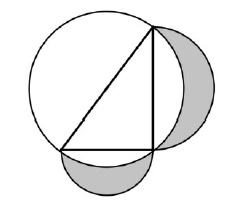
\includegraphics[scale=0.35]{rr.png}}
\end{figure}\\
154. Даны два полукруга, с диаметрами на одной прямой.
Хорда большего полукруга $AB$ длиной 12 параллельна диаметру и касается
меньшего полукруга. Найдите площадь закрашенной фигуры.
\begin{figure}[h]
\center{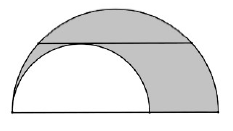
\includegraphics[scale=0.35]{rrr.png}}
\end{figure}\\
155. В трапеции $ABCD$ нижнее основание $AD$ в три раза больше верхнего. Точка $M$ лежит на боковой
стороне $CD,$ причём $CM:MD=1:3.$ Отрезок $AM$ пересекает диагональ $BD$ в точке $O.$ Найдите, в
каком отношении точка $O$ делит каждый из этих отрезков.\\
156. В треугольнике $ABC$ на стороне $BC$ взята точка $N,$ такая, что $BN : NC=3:2.$ Отрезок $AN$ и медиана
$BM$ пересекаются в точке $O.$ Найдите, в каком отношении точка $O$ делит каждый из этих отрезков.\\
157. Прямая, проведенная через середину $N$ стороны $AB$ квадрата $ABCD,$ пересекает сторону $AD$ в точке
$T,$ а продолжение стороны $CD$ в точке $M,$ и образует с прямой $AB$ угол, тангенс которого равен 0,5.
Сторона квадрата равна 8. Найдите площадь треугольника $BMT.$\\
158. Прямая, проведенная через середину $N$ стороны $AB$ квадрата $ABCD,$ пересекает прямые $CD$ и
$AD$ в точках $M$ и $T$ соответственно (так, что $T$ лежит на продолжении $DA$ за точку $A),$ и
образует с прямой $AD$ угол, тангенс которого равен 2. Сторона квадрата равна 6. Найдите площадь треугольника $BMT.$\\
159. Внутри угла величиной $45^\circ$ расположена точка $N,$ удалённая на расстояния $2\sqrt{2}$ и 2 см от сторон угла.
Найдите расстояние от точки $N$ до вершины угла.\\
160. Внутри угла величиной $60^\circ$ расположена точка $M,$ удалённая на расстояния $\sqrt{7}$ и $2\sqrt{7}$ см от
сторон угла. Найдите расстояние от точки $M$ до вершины угла.\\
161. Сторона параллелограмма равна 12см, а расстояние от точки пересечения диагоналей до этой стороны равно 4см. Найдите площадь параллелограмма.\\
162. Сторона параллелограмма равна 14см, а расстояние от точки пересечения диагоналей до этой стороны равно 3см. Найдите площадь параллелограмма.\\
163. В равнобедренном треугольнике $ABC\ (AB=BC)\ AB=25,\ AC=14.$\\
а) Найдите высоту треугольника, проведённую из вершины $C.$\\
б) Найдите радиус вписанной окружности треугольника $ABC.$\\
в) Найдите радиус описанной окружности треугольника $ABC.$\\
г) В треугольник вписан прямоугольник $KLMN\ (LM=2KL)$ так, что точки $K$ и $L$ лежат на стороне $AC,$ а точки $M$ и $N$ --- на сторонах $BC$ и $AB$ соответственно. Найдите длину $KL.$\\
164. $AC$ --- основание равнобедренного треугольника $ABC.$ Точка $D$ лежит на стороне $AC.$ $AD=4,\ DC=3.$ Окружности, вписанные в треугольники $ABD$ и $DBC,$ касаются $BD$ в точках $M$ и $N$ соответственно. Найдите длину отрезка $MN.$\\
165. $PK$ --- основание равнобедренного треугольника $SPK.$ Точка $F$ лежит на стороне $PK.$ $PF=1,\ FK=3.$ Окружности, вписанные в треугольники $PSF$ и $FSK,$ касаются $SF$ в точках $E$ и $O$ соответственно. Найдите длину отрезка $OE.$\\
166. Найдите площадь прямоугольного треугольника, если биссектриса прямого угла делит гипотенузу на отрезки длины 3 и 4.\\
167. Найдите площадь прямоугольного треугольника, если биссектриса прямого угла делит гипотенузу на отрезки длины 15 и 20.\\
168. Дан $\Delta ABC$ с углами $\angle A=40^\circ,\ \angle B=120^\circ,\ \angle C=20^\circ.$ В нём проведены высоты $AA_1,\ BB_1,$\\$ CC_1,\ H$ --- точка их пересечения. Найти: а) $\angle ACH$ б) $\angle HA_1C_1$ в) $\angle A_1B_1B$\\
169. Дана трапеция $ABCD$ с основаниями 15 и 20 и боковыми сторонами 4 и 5. Две окружности касаются обоих оснований трапеции и, кроме того, одной из боковых сторон $AB$ и $CD$ соответственно. Найти расстояние между центрами окружностей.\\
170. Дан $\Delta ABC:\ AB=30,\ AC=40,\ AL$ --- биссектриса, $M$ --- середина $AL.$ Площадь $\Delta BML$ равна 60. Найти площадь $\Delta MLC.$\\
171. $ABCD$ --- параллелограмм площадью 22. $AK$ --- биссектриса острого угла $A,$ точка $K\in BC,\ AB=5,\ AD=6,\ AK\cap BD=O.$ Найти площадь $\Delta BOK.$\\
172. $ABCD$ --- трапеция с основаниями $BC$ и $AD$ площадью 20. $CK$ --- биссектриса угла $C,$ точка $K\in AD,\ BC=3,\ AD=7, CD=5,\ CK\cap BD=O.$ Найти площадь $\Delta BOC.$\\
173. $AC$ --- основание р/б $\Delta ABC,\ D\in AC,\ AD=4,\ CD=2.$ Окружности, вписанные в $\Delta ABD$ и $\Delta DBC,$ касаются $BD$ в точках $M$ и $N$ соответственно. Найти длину отрезка $MN.$\\
174. $PK$ --- основание р/б $\Delta SPK,\ F\in PK,\ FK=3.$ Окружности, вписанные в $\Delta PSF$ и $\Delta FSK,$ касаются $SF$ в точках $E$ и $O$ соответственно. Найти длину отрезка $OE.$\\
175. В треугольнике $ABC$ известны длины двух сторон $|AB|=6,\ |AC|=4.$ Биссектриса $CK$ делит медиану $AM$ пополам.\\
а) Найдите $|AK|.$\\
б) Найдите косинус наибольшего угла треугольника $ABC.$\\
в) Найдите $|AT|,$ где $T$ --- точка пересечения прямой $AM$ с описанной около $\Delta ABC$ окружностью.\\
176. В равнобедренном треугольнике $ABC$ с основанием $BC\ AB=17,\ BC=16.$ Найдите $a)$ высоту из точки $B,\ b)$ радиус вписанной окружности, $c)$ радиус описанной окружности.\\
177. В треугольнике $ABC\ AB=8,\ BC=12,\ AC=10.$ Найдите длину биссектрисы $BL.$\\
178. Сторона $AD$ вписанного четырёхугольника $ABCD$ является диаметром его описанной окружности, $M$ --- точка пересечения диагоналей, $H$ --- проекция точки $M$ на $AD.$ Докажите, что $M$ --- центр вписанной окружности треугольника $BHC.$\\
179. Точка $K$ на медиане $BM$ треугольника $ABC$ такова, что $BK:KM=3:1.$ В каком отношении прямая $CK$ делит отрезок $AB?$\\
180. Дан угол с вершиной в точке $O$ величиной $60^\circ.$ Внутри этого угла взята точка $A,$ равноудалённая от сторон угла. Известно, что $OA=8.$ Найдите длину окружности с центром в $A,$ касающейся сторон угла.\\
181. Дан угол с вершиной в точке $O$ величиной $120^\circ.$ В этот угол вписан круг площади $81\pi.$ Найдите расстояние от центра этого круга до точки $O.$\\
182. В треугольнике $ABC$ проведены медиана $BM$ и отрезок $AN,$ где точка $N$ лежит на стороне $BC,$ причём $BN:BC=0,4.$ Отрезки $BM$ и $AN$ пересекаются в точке $O.$ Найдите $BO:OM.$\\
183. В треугольнике $KLM$ проведены медиана $MA$ и отрезок $KB,$ где точка $B$ лежит на стороне $ML,$ причём $LB:BM=2:3.$ Отрезки $MA$ и $KB$ пересекаются в точке $O.$ Найдите $KO:KB.$\\
184. Площадь треугольника $ABC$ равна $5\sqrt{5},$ при этом $AB=3\sqrt{5},\ AC=2\sqrt{5}.$ Найдите периметр данного треугольника.\\
185. Площадь треугольника $ABC$ равна 32, при этом $AB=10,\ \cos(\angle A)=0,6.$ Найдите периметр данного треугольника.\\
186. В трапеции $ABCD$ с основаниями $AD$ и $BC$ известны длины всех сторон: $AB=5,\ BC=8,\ CD=4,\ AD=10.$ Найдите расстояние от точки $C$ до прямой $AB.$\\
187. В трапеции $ABCD$ даны длины оснований $AD=12$ и $BC=8,$ а также длины диагоналей $AC=10$ и $BD=18.$ Найдите расстояние от точки $D$ до прямой $AC.$\\
188. Дан треугольник $ABC,$ в котором $\angle B=90^\circ.$ Пусть $BK$ --- высота этого треугольника. Известно, что $BC=40,\ BK=24.$ Найдите расстояние между центрами окружностей, вписанных в треугольники $ABK$ и $BKC.$\\
189. Дан треугольник $ABC$ с прямым углом при вершине $B.$ Пусть $BK$ --- высота этого треугольника. Известно, что $AB=18,\ KC=19,2.$ В треугольник $BKC$ вписана окружность с центром $O.$ Найдите расстояние между точкой $O$ и центром окружности, описанной около треугольника $ABC.$\\
190. В ромбе со стороной 17 одна из диагоналей имеет длину 16. Найдите радиус вписанной в этот ромб окружности.\\
191. Из точки $X$ к окружности проведены касательная и секущая. Расстояние от $X$ до точки касания равно 9, а расстояние от $X$ до одной из точек пересечения окружности и секущей равно 27. Найдите радиус окружности, если расстояние от центра до секущей равно 5.\\
192. В треугольнике $ABC$ медиана $AM$ и биссектриса $BL$ перпендикулярны и пересекаются в точке $F.$ Найдите площадь треугольника $ABC,$ если площадь треугольника $FML$ равна 1.\\
193. Точки $M$ и $N$ --- середины сторон $AB$ и $BC$ треугольника $ABC$ соответственно, $BL$ --- его биссектриса. Оказалось, что четырёхугольник $MBNL$ вписан в окружность радиуса $8\sqrt{3},$ а $AL:LC=2:3.$ Найдите $MN.$\\
194. Основания равнобедренной трапеции равны 7 и 25, а боковые стороны --- 15. Докажите, что центр окружности, описанной около трапеции, лежит на её большем основании.\\
195. Биссектриса $AL$ треугольника $ABC$ перпендикулярна его медиане $BM.$ Найдите площадь этого треугольника, если известно, что $AB=\sqrt{3},\ ML=1.$\\
196. В четырёхугольник $ABCD$ вписана окружность. $E$ --- точка касания окружности со стороной $AB.$ Продолжения сторон $AB$ и $CD$ пересекаются в точке $P.$ Найдите длину отрезка $EP,$ если периметр $\Delta BKP$ равен 8.\\
197. В четырёхугольник $AKPC$ вписана окружность. $E$ --- точка касания окружности со стороной $AK.$ Продолжения сторон $AK$ и $PC$ пересекаются в точке $B.$ Найдите периметр $\Delta BKP,$ если $BE=7.$\\
198. Трапеция делится диагоналями на 4 треугольника с площадями $A,\ B,\ C$ и $D.$ $A=3,\ D=12.$ Найдите площадь трапеции.\\
199. Трапеция делится диагоналями на 4 треугольника с площадями $A,\ B,\ C$ и $D.$ $A=4,\ D=8.$ Найдите площадь трапеции.\\
200. Пусть $a,b,c$ --- длины сторон треугольника, $S$ --- его площадь. Докажите неравенство $6S<ab+bc+ac.$\\
201. Найдите все прямоугольные треугольники, длины сторон которых выражаются целыми числами, если известно, что гипотенуза на 1 больше одного из катетов, а косинус угла между этими сторонами меньше $\cfrac{29}{30}.$\\
202. В неравнобедренном прямоугольном треугольнике $ABC$ с прямым углом $B$ точка $C_1$ симметрична точке $C$ относительно прямой, содержащей медиану $BM.$ Найдите $\angle AC_1B,$ если $\angle BAC=\alpha.$\\
203. Площадь треугольника $ABC$ равна $S.$ Точка $M$ --- середина его стороны $BC,$ а точка $K$ делит сторону $AC$ в отношении $AK:KC=2:1.$ Отрезки $AM$ и $BK$ пересекаются в точке $O.$ Найдите площадь четырёхугольника $OMCK.$\\
204. На сторонах прямого угла с вершиной $M$ выбраны точки $D$ и $K$ так, что $MD : MK = 7.$ На
биссектрисе угла $DMK$ взята точка $E,$ равноудалённая от $D$ и $K.$ Найдите $DK,$ если $ME = 4.$\\
205. На сторонах прямого угла с вершиной $B$ выбраны точки $A$ и $C$ так, что $AB : CB = 4 : 3.$ На
биссектрисе $ABC$ взята точка $K,$ равноудалённая от $A$ и $C.$ Найдите $AC,$ если $BK =\cfrac{7\sqrt{2}}{2}.$\\
206. Боковые стороны трапеции равны 15 см и 20 см, а основания равны 6 см и 31 см. Найдите угол между прямыми, содержащими боковые стороны трапеции.\\
207. Диагонали трапеции равны 10 см и 24 см, а основания равны 7 см и 19 см. Найдите угол между прямыми, содержащими диагонали трапеции.\\
208. Круги радиусов 3, 7 и 10 касаются друг друга внешним образом. Найдите радиус окружности, вписанной в треугольник с вершинами в центрах этих кругов.\\
209. Круги радиусов 5, 6 и 9 касаются друг друга внешним образом. Найдите радиус окружности, вписанной в треугольник с вершинами в центрах этих кругов.\\
210. В $\Delta ABC:\; |AB| = 3,\ |BC| = 5,\ |CA| = 7, O$ --- центр вписанной в треугольник окружности.
Разложите вектор  $\overline{BO}$ по векторам  $\overline{AB}=\vec{b}$ и  $\overline{AC}=\vec{c}.$\\
211. В $\Delta ABC:\; |AB| = 3,\ |BC| = 5,\ |CA| = 7,\ O$ --- центр вписанной в треугольник окружности. Разложите вектор $\overline{CO}$ по векторам
$\overline{AB}=\vec{b}$ и  $\overline{AC}=\vec{c}.$\\
212. В трапеции  $ABCD$ длина основания  $AD$ равна  $2\sqrt{2},$ а длина основания  $BC$ равна  $\sqrt{2}.$ Угол $A=15^\circ,$
угол $D=30^\circ.$ Найдите длину боковой стороны  $AB.$\\
213. Высоты  $AK$ и  $CL$ остроугольного треугольника  $ABC$ пересекаются в точке  $H.$ Найдите тангенс угла
$BAC,$ если  $AH=HK$ и  $CH=2HL.$\\
214. В трапеции  $ABCD\  (AD\parallel BC)$ из точки  $E$ --- середины  $CD$ провели перпендикуляр  $EF$ к прямой  $AB.$
Найдите площадь трапеции, если  $AB=5,\ EF=4.$\\
215. На стороне  $AC$ треугольника  $ABC$ как на диаметре построена окружность радиуса 10 см. Эта
окружность пересекает стороны  $AB$ и  $BC$ в точках  $X$ и  $Y$ соответственно. Найдите  $AX\cdot AB + CY\cdot BC.$
\newpage
\section{Числовые выражения решения}
1. $ 2\sqrt{7-4\sqrt{3}}+\sqrt{13-4\sqrt{3}} = 2\sqrt{(2 - \sqrt{3})^2} + \sqrt{(2\sqrt{3} - 1)^2} = 4 - 2\sqrt{3} + 2\sqrt{3} - 1 = 3.$\\
2. $\sqrt{3-2\sqrt{2}}-\sqrt{2}+1 = \sqrt{(\sqrt{2} - 1)^2} - \sqrt{2} + 1 = (\sqrt{2} - 1) - \sqrt{2} + 1 = 0.$\\
3. Пусть $x = 1997\cfrac{19}{6891},$ тогда $1998\cfrac{19}{6891}\cdot1997\cfrac{19}{6891}-1999\cfrac{19}{6891}\cdot1996\cfrac{19}{6891}=
(x+1)x-(x+2)(x-1)=x^2+x-x^2+x-2x+2=2.$\\
4. $(\sqrt[3]{49}+\sqrt[3]{7}+1)\cdot(\sqrt[3]{49}-1)\cdot(\sqrt[3]{49}-\sqrt[3]{7}+1) = (\sqrt[3]{49}+\sqrt[3]{7}+1)\cdot(\sqrt[3]{7}+1)\cdot(\sqrt[3]{7}-1)\\\cdot(\sqrt[3]{49}-\sqrt[3]{7}+1) = (7 - 1)\cdot(7 + 1) = 49 - 1 = 48.$\\
5. $0,815 \cdot \left (-\cfrac{2}{3}\right )-\cfrac{1}{6}\cdot(-4,385)+0,815\cdot\cfrac{1}{6}-(-4,385)\cdot\left(-\cfrac{2}{3}\right)=
0,815\cdot\left(\cfrac{1}{6}-\cfrac{2}{3}\right)+4,385\cdot\left(\cfrac{1}{6}-\cfrac{2}{3}\right)=
(0,815+4,385)\left(\cfrac{1}{6}-\cfrac{2}{3}\right)=5,2\cdot\left(-\cfrac{1}{2}\right)=-2,6.$\\
6. $(-14,09)\cdot 2\cfrac{1}{6}-6,31\cdot\left (-1\cfrac{1}{2}\right )-2\cfrac{1}{6}\cdot6,31+\left(-1\cfrac{1}{2}\right)\cdot(-14,09)=
(-14,09)\cdot\left(2\cfrac{1}{6}-1\cfrac{1}{2}\right)-6,31\cdot\left(2\cfrac{1}{6}-1\cfrac{1}{2}\right)=
(-14,09-6,31)\left(2\cfrac{1}{6}-1\cfrac{1}{2}\right)=-20,4\cdot\cfrac{2}{3}=-13,6.$\\
7. $\cfrac{\sqrt{21+8\sqrt{5}}}{4+\sqrt{5}}\cdot\sqrt{9-4\sqrt{5}}=\cfrac{\sqrt{(4+\sqrt{5})^2}}{4+\sqrt{5}}\cdot\sqrt{(2-\sqrt{5})^2}=
\cfrac{4+\sqrt{5}}{4+\sqrt{5}}\cdot(\sqrt{5}-2)=\sqrt{5}-2.$\\
8. $\sqrt{19-6\sqrt{10}}\cdot\cfrac{3-\sqrt{7}}{\sqrt{16-6\sqrt{7}}}=\sqrt{(3-\sqrt{10})^2}\cdot\cfrac{3-\sqrt{7}}{\sqrt{(3-\sqrt{7})^2}}=
(\sqrt{10}-3)\cdot\cfrac{3-\sqrt{7}}{3-\sqrt{7}}=\sqrt{10}-3.$\\
9. $\sqrt{6}+\sqrt{5}-\cfrac{1}{\sqrt{11-2\sqrt{30}}}=\sqrt{6}+\sqrt{5}-\cfrac{1}{\sqrt{(\sqrt{6}-\sqrt{5})^2}}=
\sqrt{6}+\sqrt{5}-\cfrac{1}{\sqrt{6}-\sqrt{5}}=\sqrt{6}+\sqrt{5}-\cfrac{\sqrt{6}+\sqrt{5}}{6-5}=0.$\\
10. $\sqrt{7}-\sqrt{2}-\cfrac{5}{\sqrt{9+2\sqrt{14}}}=\sqrt{7}-\sqrt{2}-\cfrac{5}{\sqrt{(\sqrt{7}+\sqrt{2})^2}}=
\sqrt{7}-\sqrt{2}-\cfrac{5}{\sqrt{7}+\sqrt{2}}=\sqrt{7}-\sqrt{2}-\cfrac{5(\sqrt{7}-\sqrt{2})}{7-2}=\sqrt{7}-\sqrt{2}-\sqrt{7}+\sqrt{2}=0.$\\
11. $(-1,5)^{-3}-\left(\cfrac{2}{5}\right)^{-4}\cdot\left(\cfrac{2}{5}\right)^{3}-\left(\left(\cfrac{4}{9}\right)^{0,5}\right)^0+16^{\frac{3}{4}}\cdot0,5=
-\cfrac{8}{27}-\left(\cfrac{2}{5}\right)^{-1}-1+8\cdot0,5=
-\cfrac{8}{27}-\cfrac{5}{2}-1+4=\cfrac{11}{54}.$\\
12. $\left(\cfrac{3}{5}\right)^{-3}\cdot\left(\cfrac{3}{5}\right)^{4}-\left(\left(\cfrac{9}{25}\right)^{0}\right)^{0,5}-(-0,5)^{-3}-25^{1,5}\cdot0,2=
\cfrac{3}{5}-1+8-125\cdot0,2=-\cfrac{87}{5}.$\\
13. $(-1)^{21}-81^\frac{3}{4}+\left(2^\frac{2}{3}\cdot2^\frac{1}{2}\right)^6-16^{\frac{5}{4}}+\left(-\cfrac{1}{4}\right)^{-3}=
-1-27+\left(2^\frac{7}{6}\right)^6-32-64=-1-27+128-32-64=4.$\\
14. $(-1)^{18}+32^\frac{4}{5}+8\cdot27^\frac{1}{3}-\cfrac{1}{27}\cdot\left(3^\frac{1}{4}\cdot3^\frac{1}{3}\right)^{12}-\left(-\cfrac{1}{6}\right)^{-3}=
1+16+8\cdot3-\cfrac{1}{27}\cdot 3^\frac{7}{12}\cdot12+216=
1+16+24-81+216=176.$\\
15. $(\sqrt{2}-\sqrt{3})\sqrt{5+2\sqrt{6}}=(\sqrt{2}-\sqrt{3})\sqrt{(\sqrt{2}+\sqrt{3})^2}=(\sqrt{2}-\sqrt{3})(\sqrt{2}+\sqrt{3})=2-3=-1.$\\
16. $(\sqrt{5}-\sqrt{6})\sqrt{11+2\sqrt{30}}=(\sqrt{5}-\sqrt{6})\sqrt{(\sqrt{5}+\sqrt{6})^2}=(\sqrt{5}-\sqrt{6})(\sqrt{5}+\sqrt{6})=5-6=-1.$\\
17. $\cfrac{\left(5\cfrac{4}{45}-4\cfrac{1}{6}\right):5\cfrac{8}{15}}{\left(4\cfrac{2}{3}+0,75\right)\cdot3\cfrac{9}{13}}
\cdot34\cfrac{2}{7}+\cfrac{0,3:0,01}{70}+\cfrac{2}{7}=\cfrac{\cfrac{83}{90}:\cfrac{83}{15}}{\cfrac{65}{12}\cdot\cfrac{48}{13}}
\cdot\cfrac{240}{7}+\cfrac{3}{7}+\cfrac{2}{7}=\cfrac{\cfrac{1}{6}}{20}
\cdot\cfrac{240}{7}+\cfrac{5}{7}=\cfrac{2}{7}+\cfrac{5}{7}=1.$\\
18. $\cfrac{\left(\cfrac{3}{5}+0,425-0,005\right):0,1}{30,5+\cfrac{1}{6}+3\cfrac{1}{3}}+
\cfrac{6\cfrac{3}{4}+5\cfrac{1}{2}}{26:3\cfrac{5}{7}}-0,05=\cfrac{\left(0,6+0,42\right)\cdot10}{30,5+3,5}+
\cfrac{\cfrac{49}{4}}{26:\cfrac{26}{7}}-0,05=\cfrac{10,2}{34}+\cfrac{\cfrac{49}{4}}{7}-0,05=
0,3+1,75-0,05=2.$\\
19. $\cfrac{10}{\sqrt{5}-\sqrt{10}+\sqrt{20}+\sqrt{40}-\sqrt{80}}=\cfrac{10}{\sqrt{5}-\sqrt{10}+2\sqrt{5}+2\sqrt{10}-4\sqrt{5}}=
\cfrac{10}{\sqrt{10}-\sqrt{5}}=\cfrac{10(\sqrt{10}+\sqrt{5})}{10-5}=2(\sqrt{5}+\sqrt{10}).$\\
20. $\cfrac{\sqrt{6}}{\sqrt{3}-\sqrt{6}-\sqrt{24}-\sqrt{48}+\sqrt{108}}=\cfrac{\sqrt{6}}{\sqrt{3}-\sqrt{6}-2\sqrt{6}-4\sqrt{3}+6\sqrt{3}}=
\cfrac{\sqrt{6}}{3(\sqrt{3}-\sqrt{6})}=\cfrac{\sqrt{6}(\sqrt{3}+\sqrt{6})}{3(3-6)}=
-\cfrac{3(\sqrt{2}+2)}{9}=-\cfrac{1}{3}(2+\sqrt{2}).$\\
21. $\cfrac{7,46^3+6,26^3}{13,72}-7,46\cdot 6,26=[x=7,46,\ y=6,26]=\cfrac{x^3+y^3}{x+y}-xy=
x^2-xy+y^2-xy=(x-y)^2=(7,46-6,26)^2=1,44.$\\
22. $\cfrac{2,5^3-4,4^3}{1,9}+2,5^2+4,4^2=[x=2,5,\ y=4,4]=\cfrac{x^3-y^3}{y-x}+x^2+y^2=
-x^2-xy-y^2+x^2+y^2=-xy=-2,5\cdot4,4=-11.$\\
23. $\cfrac{3\cfrac{1}{3}\cdot1,9+19,5:4\cfrac{1}{2}}{\cfrac{62}{75}-0,16}:\cfrac{3,5+4\cfrac{2}{3}+2\cfrac{2}{15}}{0,5\cdot\left(1\cfrac{1}{20}+4,1\right)}=
\cfrac{\cfrac{10}{3}\cdot\cfrac{19}{10}+\cfrac{195}{10}:\cfrac{9}{2}}{\cfrac{62}{75}-\cfrac{16}{100}}:\cfrac{3,5+6,8}{0,5\cdot5,15}=
\cfrac{\cfrac{19}{3}+\cfrac{13}{3}}{\cfrac{2}{3}}:\cfrac{10,3}{2,575}=
\cfrac{\cfrac{32}{3}}{\cfrac{2}{3}}:4=16:4=4.$\\
24. $2\sqrt{3}+0,25(\sqrt{21}-5)(\sqrt{7}+3\sqrt{3})+\cfrac{2\sqrt{7}-4}{1+\sqrt{7}}=
2\sqrt{3}+0,25(7\sqrt{3}+9\sqrt{7}-5\sqrt{7}-15\sqrt{3})+$\\$\cfrac{(2\sqrt{7}-4)(\sqrt{7}-1)}{7-1}=
2\sqrt{3}+0,25(4\sqrt{7}-8\sqrt{3})+\cfrac{14-2\sqrt{7}-4\sqrt{7}+4}{6}=
2\sqrt{3}+\sqrt{7}-2\sqrt{3}+3-\sqrt{7}=3.$\\
25. $\cfrac{1-\sqrt{10}}{\sqrt{2}+\sqrt{5}}+\cfrac{7}{2\sqrt{2}+1}-(11-5\sqrt{5})(2+\sqrt{5})=
\cfrac{(1-\sqrt{10})(\sqrt{5}-\sqrt{2})}{5-2}+\cfrac{7(2\sqrt{2}-1)}{8-1}-22-11\sqrt{5}+10\sqrt{5}+25=
\cfrac{\sqrt{5}-\sqrt{2}-5\sqrt{2}+2\sqrt{5}}{3}+2\sqrt{2}-1+3-\sqrt{5}=\sqrt{5}-2\sqrt{2}+2\sqrt{2}+2-\sqrt{5}=2.$\\
26. $(36,5^2-27,5^2):\left(\cfrac{57^3+33^3}{90}-57\cdot 33 \right)=
(36,5-27,5)(36,5+27,5):\left(57^2-57\cdot33+33^2-57\cdot 33 \right)=\cfrac{9\cdot64}{(57-33)^2}=\cfrac{9\cdot64}{24^2}=1.$\\
27. $\left(\cfrac{97^3-53^3}{44}+97\cdot53\right):(152,5^2-27,5^2)=(97^2+97\cdot53+53^2+97\cdot53):((152,5-27,5)(152,5+27,5))=
\cfrac{(97+53)^2}{125\cdot180}=\cfrac{150^2}{125\cdot180}=1.$\\
28. $\cfrac{\sqrt{7-4\sqrt{3}}}{\sqrt{2-\sqrt{3}}}\sqrt{2+\sqrt{3}}=
\cfrac{\sqrt{(2-\sqrt{3})^2}}{\sqrt{2-\sqrt{3}}}\sqrt{2+\sqrt{3}}=\cfrac{2-\sqrt{3}}{\sqrt{2-\sqrt{3}}}\sqrt{2+\sqrt{3}}=
\sqrt{2-\sqrt{3}}\sqrt{2+\sqrt{3}}=$\\$\sqrt{(2-\sqrt{3})(2+\sqrt{3})}=\sqrt{4-3}=1.$\\
29. $\cfrac{\sqrt{7+4\sqrt{3}}}{\sqrt{2+\sqrt{3}}}\sqrt{2-\sqrt{3}}=
\cfrac{\sqrt{(2+\sqrt{3})^2}}{\sqrt{2+\sqrt{3}}}\sqrt{2-\sqrt{3}}=
\cfrac{2+\sqrt{3}}{\sqrt{2+\sqrt{3}}}\sqrt{2-\sqrt{3}}=\sqrt{2+\sqrt{3}}\sqrt{2-\sqrt{3}}=$\\$\sqrt{(2+\sqrt{3})(2-\sqrt{3})}=\sqrt{4-3}=1.$\\
30. $\left(\cfrac{1}{\sqrt{5}+\sqrt{6}}+\cfrac{1}{\sqrt{5}-2}\right):\left(1+\cfrac{\sqrt{6}}{2}\right)=
\left(\cfrac{\sqrt{6}-\sqrt{5}}{6-5}+\cfrac{\sqrt{5}+2}{5-4}\right):\cfrac{2+\sqrt{6}}{2}=
\left(\sqrt{6}-\sqrt{5}+\sqrt{5}+2\right)\cdot\cfrac{2}{2+\sqrt{6}}=(2+\sqrt{6})\cdot\cfrac{2}{2+\sqrt{6}}=2.$\\
31. $\left(\cfrac{1}{\sqrt{10}+\sqrt{11}}+\cfrac{1}{\sqrt{10}-3}\right):\left(1+\cfrac{\sqrt{11}}{3}\right)=
\left(\cfrac{\sqrt{11}-\sqrt{10}}{11-10}+\cfrac{\sqrt{10}+3}{10-9}\right):\cfrac{3+\sqrt{11}}{3}=$\\$
\left(\sqrt{11}-\sqrt{10}+\sqrt{10}+3\right)\cdot\cfrac{3}{3+\sqrt{11}}=
(3+\sqrt{11})\cdot\cfrac{3}{3+\sqrt{11}}=3.$\\
32. $\sqrt[6]{31+10\sqrt{6}}\cdot\sqrt[3]{5-\sqrt{6}}=\sqrt[6]{(5+\sqrt{6})^2}\cdot\sqrt[3]{5-\sqrt{6}}=\sqrt[3]{5+\sqrt{6}}\cdot\sqrt[3]{5-\sqrt{6}}=
\sqrt[3]{(5+\sqrt{6})(5-\sqrt{6})}=\sqrt[3]{25-6}=\sqrt[3]{19}.$\\
33. $\sqrt{175}-3\sqrt{3\cfrac{1}{9}}-6\sqrt{1,75}=5\sqrt{7}-3\sqrt{\cfrac{28}{9}}-6\sqrt{\cfrac{175}{100}}=
5\sqrt{7}-3\cdot\cfrac{2\sqrt{7}}{3}-6\cdot\cfrac{5\sqrt{7}}{10}=5\sqrt{7}-2\sqrt{7}-3\sqrt{7}=0.$\\
34. $\left(\cfrac{\sqrt[3]{\sqrt{3}+\sqrt{6}}\sqrt[6]{9-6\sqrt{2}}-\sqrt[6]{18}}{\sqrt[6]{2}-1}\right)^3=
\left(\cfrac{\sqrt[6]{3+2\sqrt{18}+6}\sqrt[6]{9-6\sqrt{2}}-\sqrt[6]{2}\sqrt[6]{9}}{\sqrt[6]{2}-1}\right)^3=$\\$
\left(\cfrac{\sqrt[6]{(9+6\sqrt{2})(9-6\sqrt{2})}-\sqrt[6]{2}\sqrt[6]{9}}{\sqrt[6]{2}-1}\right)^3=
\left(\cfrac{\sqrt[6]{81-72}-\sqrt[6]{2}\sqrt[6]{9}}{\sqrt[6]{2}-1}\right)^3=
\left(\cfrac{\sqrt[6]{9}(1-\sqrt[6]{2})}{\sqrt[6]{2}-1}\right)^3=
\left(-\sqrt[6]{9}\right)^3=-\sqrt{9}=-3.$\\
35. $\cfrac{1}{\sqrt[3]{25}+\sqrt[3]{5}+1}=\cfrac{\sqrt[3]{5}-1}{5-1}=\cfrac{1}{4}(\sqrt[3]{5}-1).$\\
36. $\cfrac{1}{\sqrt[3]{9}-2\sqrt[3]{3}+4}=\cfrac{\sqrt[3]{3}+2}{3+8}=\cfrac{1}{11}(\sqrt[3]{3}+2).$\\
37. а) $\cfrac{1}{\sqrt{3}-\sqrt{2}}=\cfrac{\sqrt{3}+\sqrt{2}}{3-2}=\sqrt{3}+\sqrt{2}>\sqrt{2}+\sqrt{2}=2\sqrt{2}.$\\
б) $\sqrt{10}-\sqrt{11}??\sqrt{12}-\sqrt{13},\ \sqrt{10}+\sqrt{13}??\sqrt{11}+\sqrt{12},\ 10+2\sqrt{130}+13??11+2\sqrt{132}+12,\ 23+2\sqrt{130}<23+2\sqrt{132}.$\\
38. $27894^2+1618^2??27895^2+1617^2,\ 1618^2-1617^2??27895^2-27894^2,\ (1618-1617)(1618+1617)??(27895-27894)(27895+27894),\ 1618+1617<27895+27894.$\\
39. Пусть $x=191,$ тогда $B=(x-3)(x-2)(x-1)(x+1)(x+2)(x+3)=(x^2-1)(x^2-4)(x^2-9)<x^2 \cdot x^2\cdot x^2=x^6=191^6=A.$\\
40. $(2-\sqrt{5})\sqrt{9+4\sqrt{5}}=-\sqrt{(4-4\sqrt{5}+5)(9+4\sqrt{5})}=-\sqrt{(9-4\sqrt{5})(9+4\sqrt{5})}=-\sqrt{81-80}=-1.$\\
41. $(\sqrt{7}-3)\sqrt{16+6\sqrt{7}}=-\sqrt{(7-6\sqrt{7}+9)(16+6\sqrt{7})}=-\sqrt{(16-6\sqrt{7})(16+6\sqrt{7})}=-\sqrt{256-252}=-2.$\\
42. $74,7\cdot\cfrac{2}{21}+(-105,3)\cdot2\cfrac{3}{7}-(-105,3)\cdot\cfrac{2}{21}-2\cfrac{3}{7}\cdot74,7=74,7\cdot\left(\cfrac{2}{21}-\cfrac{17}{7}\right)+105,3
\cdot\left(\cfrac{2}{21}-\cfrac{17}{7}\right)=\left(\cfrac{2}{21}-\cfrac{17}{7}\right)(74,7+105,3)=-\cfrac{49}{21}\cdot180=-420.$\\
43. $6\cfrac{1}{10}\cdot2,391-0,109\cdot1\cfrac{5}{6}-1\cfrac{5}{6}\cdot2,391+0,109\cdot6\cfrac{1}{10}=
2,391\cdot\left(6\cfrac{1}{10}-1\cfrac{5}{6}\right)+0,109\cdot\left(6\cfrac{1}{10}-1\cfrac{5}{6}\right)=
\left(\cfrac{61}{10}-\cfrac{11}{6}\right)(2,391+0,109)=\cfrac{128}{30}\cdot2,5=\cfrac{32}{3}.$\\
44. Возведём оба числа в 6 степень: $(\sqrt{4+\sqrt{7}}-\sqrt{4-\sqrt{7}})^6=(4+\sqrt{7}-2\cdot\sqrt{16-7}+4-\sqrt{7})^3=2^3=8,\ (\sqrt[3]{2})^6=2^2=4.$ Значит, первое число больше.\\
45. $\cfrac{2}{\sqrt{8-2\sqrt{15}}}-\cfrac{1}{\sqrt{22-4\sqrt{30}}}-\sqrt{5}=\cfrac{2}{\sqrt{(\sqrt{5}-\sqrt{3})^2}}-\cfrac{1}{\sqrt{(\sqrt{12}-\sqrt{10})^2}}-\sqrt{5}=
\cfrac{2}{\sqrt{5}-\sqrt{3}}-\cfrac{1}{\sqrt{12}-\sqrt{10}}-\sqrt{5}=\sqrt{5}+\sqrt{3}-\cfrac{1}{2}(\sqrt{12}+\sqrt{10})-\sqrt{5}=-\cfrac{\sqrt{10}}{2}.$\\
46.$\cfrac{10\sqrt{5}}{{\sqrt{38-12\sqrt{10}}+\sqrt{18}}}=\cfrac{10\sqrt{5}}{{\sqrt{(2\sqrt{5}-3\sqrt{2})^2}+3\sqrt{2}}}=[(2\sqrt{5})^2=20>18=(3\sqrt{2})^2 ]=$\\$\cfrac{10\sqrt{5}}{2\sqrt{5}-3\sqrt{2}+3\sqrt{2}}=\cfrac{10\sqrt{5}}{2\sqrt{5}}=5.$\\
47. $\sqrt{\left(\cfrac{4^5}{16^{-2}\cdot2^{19}}\right)^{-1}}\cdot\sqrt{8}-(0,3)^{-1}+(2\sqrt{3})^{-2}=
\sqrt{\left(\cfrac{2^{10}}{2^{-8}\cdot2^{19}}\right)^{-1}}\cdot\sqrt{8}-\cfrac{10}{3}+\cfrac{1}{12}=
\sqrt{2}\cdot\sqrt{8}-\cfrac{13}{4}=4-\cfrac{13}{4}=\cfrac{3}{4}=0,75.$\\
48. $\sqrt{\left(\cfrac{9^{12}}{3^{-5}\cdot27^{10}}\right)^{-1}}:\sqrt{27}+(\sqrt{6})^{-2}-(1,25)^{-1}=
\sqrt{\left(\cfrac{3^{24}}{3^{-5}\cdot3^{30}}\right)^{-1}}:\sqrt{27}+\cfrac{1}{6}-\cfrac{4}{5}=
\sqrt{3}:\sqrt{27}-\cfrac{19}{30}=\cfrac{1}{3}-\cfrac{19}{30}=-\cfrac{3}{10}=-0,3.$\\
49. $\sqrt{3}+\sqrt{7}\ ??\ 9-\sqrt{21},\ 3+2\sqrt{21}+7\ ??\ 81-18\sqrt{21}+21,\ 20\sqrt{21}\ ??\ 92,\ 8400 <8464,$ значит второе число больше.\\
50. $(\sqrt[3]{49}+\sqrt[3]{7}+1)(\sqrt[3]{49}-1)(\sqrt[3]{49}-\sqrt[3]{7}+1)=[t=\sqrt[3]{7}]=(t^2+t+1)(t^2-1)(t^2-t+1)=
(t^2+t-1)(t-1)(t+1)(t^2-t+1)=(t^3+1)(t^3-1)=t^6-1=(\sqrt[3]{7})^6-1=49-1=48.$\\
51. $(\sqrt[3]{36}+\sqrt[3]{6}+1)(\sqrt[3]{36}-1)(\sqrt[3]{36}-\sqrt[3]{6}+1)=[t=\sqrt[3]{6}]=(t^2+t+1)(t^2-1)(t^2-t+1)=
(t^2+t-1)(t-1)(t+1)(t^2-t+1)=(t^3+1)(t^3-1)=t^6-1=(\sqrt[3]{6})^6-1=36-1=35.$\\
52. $\cfrac{\sqrt[4]{7\cdot\sqrt[3]{54}+15\cdot\sqrt[3]{128}}}{\sqrt[3]{4\cdot\sqrt[4]{32}}+\sqrt[3]{9\cdot\sqrt[4]{162}}}=
\cfrac{\sqrt[4]{21\sqrt[3]{2}+60\sqrt[3]{2}}}{\sqrt[3]{8\sqrt[4]{2}}+\sqrt[3]{27\sqrt[4]{2}}}=
\cfrac{\sqrt[4]{81\sqrt[3]{2}}}{2\sqrt[12]{2}+3\sqrt[12]{2}}=
\cfrac{3\sqrt[12]{2}}{5\sqrt[12]{2}}=\cfrac{3}{5}.$\\
53. $\cfrac{5\cdot\sqrt[3]{4\cdot\sqrt[3]{192}}+7\cdot\sqrt[3]{18\cdot\sqrt[3]{81}}}{\sqrt[3]{12\cdot
\sqrt[3]{24}+6\cdot\sqrt[3]{375}}}=\cfrac{5\cdot\sqrt[3]{16\sqrt[3]{3}}+7\cdot\sqrt[3]{54\sqrt[3]{3}}}{\sqrt[3]{24
\sqrt[3]{3}+30\sqrt[3]{3}}}=\cfrac{10\cdot\sqrt[3]{2\sqrt[3]{3}}+21\cdot\sqrt[3]{2\sqrt[3]{3}}}{\sqrt[3]{54
\sqrt[3]{3}}}=\cfrac{31\cdot\sqrt[3]{2\sqrt[3]{3}}}{3\cdot\sqrt[3]{2\sqrt[3]{3}}}=
\cfrac{31}{3}.$
\newpage
\section{Преобразование буквенных выражений решения}
1. $\left(\left(\cfrac{\sqrt{a}+\sqrt{b}}{\sqrt[4]{a}-\sqrt[4]{b}}\right)^{-1}-
\cfrac{2\sqrt[4]{ab}}{b^{\frac{3}{4}}-a^{\frac{1}{4}}b^{\frac{1}{2}}+
a^{\frac{1}{2}}b^{\frac{1}{4}}-a^{\frac{3}{4}}}\right)^{-1}=[x=\sqrt[4]{a},\ y=\sqrt[4]{b}]=$\\$
\left(\cfrac{x-y}{x^2+y^2}-\cfrac{2xy}{y^3-xy^2+x^2y-x^3}\right)^{-1}=
\left(\cfrac{x-y}{x^2+y^2}-\cfrac{2xy}{y^2(y-x)+x^2(y-x)}\right)^{-1}=$\\$
\left(\cfrac{x-y}{x^2+y^2}-\cfrac{2xy}{(y-x)(x^2+y^2)}\right)^{-1}=
\left(\cfrac{x-y}{x^2+y^2}+\cfrac{2xy}{(x-y)(x^2+y^2)}\right)^{-1}=
\left(\cfrac{x^2-2xy+y^2+2xy}{(x-y)(x^2+y^2)}\right)^{-1}=$\\$x-y=\sqrt[4]{a}-\sqrt[4]{b}.$\\
2. $a^{\frac{4}{3}}\cdot\left(\cfrac{3}{\sqrt[3]{a^2}-\sqrt[3]{a}+1}-
\cfrac{3}{a+1}+\cfrac{\sqrt[3]{a}-1}{\sqrt[3]{a^2}-1}\right)^{-1}
\left(\cfrac{a^{-\frac{1}{3}}+1}{a^\frac{1}{3}}\right)^2=[x=\sqrt[3]{a}]=$\\$
x^4\cdot\left(\cfrac{3}{x^2-x+1}-\cfrac{3}{x^3+1}+\cfrac{x-1}{x^2-1}\right)^{-1}\left(\cfrac{\cfrac{1}{x}+1}{x}\right)^2=$\\$
x^4\cdot\left(\cfrac{3}{x^2-x+1}-\cfrac{3}{(x+1)(x^2-x+1)}+\cfrac{1}{x+1}\right)^{-1}\left(\cfrac{x+1}{x^2}\right)^2=$\\$
x^4\cdot\left(\cfrac{3x+3-3+x^2-x+1}{(x+1)(x^2-x+1)}\right)^{-1}\cfrac{(x+1)^2}{x^4}=
\left(\cfrac{(x+1)^2}{(x+1)(x^2-x+1)}\right)^{-1}(x+1)^2=\cfrac{x^3+1}{(x+1)^2}(x+1)^2=x^3+1=a+1.$\\
3. $\left(\cfrac{n-m}{\sqrt{n}+\sqrt{m}}\right)^2:\left(\cfrac{\sqrt{n^3}-\sqrt{m^3}}{\sqrt{n}-\sqrt{m}}-3\sqrt{mn}\right)=
[x=\sqrt{n},\ y=\sqrt{m}]=\left(\cfrac{x^2-y^2}{x+y}\right)^2:\left(\cfrac{x^3-y^3}{x-y}-3xy\right)=
\left(x-y\right)^2:\left(x^2+xy+y^2-3xy\right)=(x-y)^2:(x-y)^2=1.$\\
4. $\left(\cfrac{\sqrt{a^3}-\sqrt{b^3}}{\sqrt{a}-\sqrt{b}}+\sqrt{ab}\right)\left(\cfrac{\sqrt{a}-\sqrt{b}}{a-b}\right)^2=[x=\sqrt{a},\ y=\sqrt{b}]=
\left(\cfrac{x^3-y^3}{x-y}+xy\right)\left(\cfrac{x-y}{x^2-y^2}\right)^2=(x^2+xy+y^2+xy)\left(\cfrac{1}{x+y}\right)^2=
(x+y)^2\cfrac{1}{(x+y)^2}=1.$\\
5. $\left(\cfrac{\sqrt[4]{ab^3}-\sqrt[4]{a^3b}}{\sqrt{a}-\sqrt{b}}\right)^{-2}\cdot\sqrt{1+\cfrac{a}{b}+2\sqrt{\cfrac{a}{b}}}=[x=\sqrt[4]{a},\ y=\sqrt[4]{b}]=
\left(\cfrac{xy^3-x^3y}{x^2-y^2}\right)^{-2}\cdot\sqrt{1+\cfrac{x^4}{y^4}+2\cfrac{x^2}{y^2}}=
\left(\cfrac{-xy(x^2-y^2)}{x^2-y^2}\right)^{-2}\cdot\sqrt{\left(1+\cfrac{x^2}{y^2}\right)^2}=
\cfrac{1}{x^2y^2}\cdot\cfrac{x^2+y^2}{y^2}=\cfrac{x^2+y^2}{x^2y^4}=\cfrac{\sqrt{a}+\sqrt{b}}{b\sqrt{a}}.$\\
6. $\left((\sqrt[4]{a}-\sqrt[4]{b})^{-1}+(\sqrt[4]{a}+\sqrt[4]{b})^{-1}\right)^{-2}:\cfrac{a-b}{4(\sqrt{a}+\sqrt{b})}=[x=\sqrt[4]{a},\ y=\sqrt[4]{b}]=
\left((x-y)^{-1}+(x+y)^{-1}\right)^{-2}:\cfrac{x^4-y^4}{4(x^2+y^2)}=
\left(\cfrac{1}{x-y}+\cfrac{1}{x+y}\right)^{-2}\cdot\cfrac{4(x^2+y^2)}{(x^2-y^2)(x^2+y^2)}=
\left(\cfrac{x+y+x-y}{(x-y)(x+y)}\right)^{-2}\cdot\cfrac{4}{x^2-y^2}=
\cfrac{(x-y)^2(x+y)^2}{4x^2}\cdot\cfrac{4}{(x-y)(x+y)}=\cfrac{x^2-y^2}{x^2}=\cfrac{\sqrt{a}-\sqrt{b}}{\sqrt{a}}.$\\
7. $\left(\sqrt{y}-\cfrac{x}{\sqrt{y}}\right):\left(\sqrt{\cfrac{x}{y}}-\sqrt{\cfrac{y}{x}}\right)=[a=\sqrt{x},\ b=\sqrt{y}]=
\left(b-\cfrac{a^2}{b}\right):\left(\cfrac{a}{b}-\cfrac{b}{a}\right)=\cfrac{b^2-a^2}{b}:\cfrac{a^2-b^2}{ab}=-a=-\sqrt{x}.$\\
8. $\left(\cfrac{y}{\sqrt{x}}-\sqrt{x}\right):\left(\sqrt{\cfrac{x}{y}}-\sqrt{\cfrac{y}{x}}\right)=[a=\sqrt{x},\ b=\sqrt{y}]=
\left(\cfrac{b^2}{a}-a\right):\left(\cfrac{a}{b}-\cfrac{b}{a}\right)=
\cfrac{b^2-a^2}{a}:\cfrac{a^2-b^2}{ab}=-b=-\sqrt{y}.$\\
9. $\cfrac{\sqrt{a-2\sqrt{a-1}}}{1-\sqrt{a-1}}=\cfrac{\sqrt{a-1-2\sqrt{a-1}+1}}{1-\sqrt{a-1}}=\cfrac{\sqrt{(\sqrt{a-1}-1)^2}}{1-\sqrt{a-1}}=
\cfrac{\sqrt{a-1}-1}{1-\sqrt{a-1}}=-1.$\\
10. $\cfrac{\sqrt{a-2\sqrt{a-1}}}{1-\sqrt{a-1}}=\cfrac{\sqrt{a-1-2\sqrt{a-1}+1}}{1-\sqrt{a-1}}\cfrac{\sqrt{(\sqrt{a-1}-1)^2}}{1-\sqrt{a-1}}=
\cfrac{1-\sqrt{a-1}}{1-\sqrt{a-1}}=1.$\\
11. $\cfrac{x-y}{\sqrt{x}+\sqrt{y}}:\left(\left(x^\frac{1}{4}-y^\frac{1}{4}\right)^{-1}+\left(x^\frac{1}{4}+y^\frac{1}{4}\right)^{-1}\right)^{-2}=[a=x^{\frac{1}{4}},\ b=y^\frac{1}{4}]=\cfrac{a^4-b^4}{a^2+b^2}:\left(\cfrac{1}{a-b}+\cfrac{1}{a+b}\right)^{-2}=
(a^2-b^2)\cdot\left(\cfrac{a+b+a-b}{a^2-b^2}\right)^{2}=(a^2-b^2)\cfrac{4a^2}{(a^2-b^2)^2}=\cfrac{4a^2}{a^2-b^2}=\cfrac{4\sqrt{x}}{\sqrt{x}-\sqrt{y}}.$\\
12. $\left(\cfrac{1}{\left(a^\frac{1}{2}+b^\frac{1}{2}\right)^{-2}}-\left(\cfrac{\sqrt{a}-\sqrt{b}}{a^\frac{3}{2}-b^\frac{3}{2}}\right)^{-1}\right):\sqrt{ab}=
[a=x^{\frac{1}{2}},\ b=y^\frac{1}{2}]=\left(\cfrac{1}{\left(x+y\right)^{-2}}-\left(\cfrac{x-y}{x^3-y^3}\right)^{-1}\right):(xy)=
\left(x^2+2xy+y^2-x^2-xy-y^2\right):(xy)=1.$\\
13. $(1-a^2):\left(\left(\cfrac{1-a\sqrt{a}}{1-\sqrt{a}}+\sqrt{a}\right)\cdot\left(\cfrac{1+a\sqrt{a}}{1+\sqrt{a}}-\sqrt{a}\right)\right)+1=[x=\sqrt{a}]=$\\$
(1-x^4):\left(\left(\cfrac{1-x^3}{1-x}+x\right)\cdot\left(\cfrac{1+x^3}{1+x}-x\right)\right)+1=
(1-x^4):\left(\left(1+x+x^2+x\right)\cdot\left(1-x+x^2-x\right)\right)+1=
(1-x^4):\left((1+x)^2\cdot(1-x)^2\right)+1=(1+x^2)(1-x^2):(1-x^2)^2+1=\cfrac{1+x^2}{1-x^2}+1=\cfrac{2}{1-x^2}=\cfrac{2}{1-a}.$\\
14. $\cfrac{(\sqrt{x}-\sqrt{y})^3+\cfrac{2x^2}{\sqrt{x}}+y\sqrt{y}}{x\sqrt{x}+y\sqrt{y}}+\cfrac{3\sqrt{xy}-3y}{x-y}=[a=\sqrt{x},\ b=\sqrt{y}]=
\cfrac{(a-b)^3+\cfrac{2a^4}{a}+b^3}{a^3+b^3}+\cfrac{3ab-3b^2}{a^2-b^2}=
\cfrac{a^3-3a^2b+3ab^2-b^3+2a^3+b^3}{a^3+b^3}+\cfrac{3b(a-b)}{(a-b)(a+b)}=
\cfrac{3a(a^2-ab+b^2)}{(a+b)(a^2-ab+b^2)}+\cfrac{3b}{a+b}=\cfrac{3a+3b}{a+b}=3.$\\
15. $\left(\cfrac{27^\frac{1}{2}-a^{-\frac{3}{2}}}{3^\frac{1}{2}-a^{-\frac{1}{2}}}+3^{\frac{1}{2}} a^{-\frac{1}{2}}
\right):(3-a^{-1})-\cfrac{2a^{-\frac{1}{2}}}{3^\frac{1}{2}-a^{-\frac{1}{2}}}=[x=3^{\frac{1}{2}},\ y=a^{-\frac{1}{2}}]=
\left(\cfrac{x^3-y^3}{x-y}+xy\right):(x^2-y^2)-\cfrac{2y}{x-y}=\cfrac{x^2+xy+y^2+xy}{(x-y)(x+y)}-\cfrac{2y}{x-y}=
\cfrac{(x+y)^2}{(x-y)(x+y)}-\cfrac{2y}{x-y}=\cfrac{x+y-2y}{x-y}=1.$\\
16. $\left(\cfrac{8^\frac{1}{2}+y^{-\frac{3}{2}}}{2^\frac{1}{2}+y^{- \frac{1}{2}}}-
2^\frac{1}{2}y^{-\frac{1}{2}}\right):(2-y^{-1})+\cfrac{2y^{-\frac{1}{2}}}{2^\frac{1}{2}+y^{-\frac{1}{2}}}=[x=2^{\frac{1}{2}},\ z=y^{-\frac{1}{2}}]=
\left(\cfrac{x^3+z^3}{x+z}-xz\right):(x^2-z^2)+\cfrac{2z}{x+z}=\cfrac{x^2-xz+z^2-xz}{(x-z)(x+z)}+\cfrac{2z}{x+z}=
\cfrac{(x-z)^2}{(x-z)(x+z)}+\cfrac{2z}{x+z}=\cfrac{x-z+2z}{x+z}=1.$\\
17. $\left(\cfrac{x-9}{x+3\sqrt{x}+9}\cdot\left(\cfrac{x^{0,5}+3}{x^{1,5}-27}\right)^{-1}\right)^{0,5}+x^{0,5}=[a=\sqrt{x}]=
\left(\cfrac{a^2-9}{a^2+3a+9}\cdot\left(\cfrac{a+3}{a^3-27}\right)^{-1}\right)^{0,5}+a=
\left(\cfrac{(a-3)(a+3)}{a^2+3a+9}\cdot\cfrac{(a-3)(a^2+3a+9)}{a+3}\right)^{0,5}+a=((a-3)^2)^{0,5}+a=3-a+a=3.$\\
18. $\left(\cfrac{a^\frac{3}{2}-8}{a^\frac{1}{2}+2}\cdot\left(\cfrac{a+2\sqrt{a}+4}{a-4}\right)^{-1}\right)^\frac{1}{2}-a^\frac{1}{2}=[x=a^\frac{1}{2}]=
\left(\cfrac{x^3-8}{x+2}\cdot\left(\cfrac{x^2+2x+4}{x^2-4}\right)^{-1}\right)^\frac{1}{2}-x=$\\$
\left(\cfrac{(x-2)(x^2+2x+4)}{x+2}\cdot\cfrac{(x-2)(x+2)}{x^2+2x+4}\right)^\frac{1}{2}-x=((x-2)^2)^\frac{1}{2}-x=x-2-x=-2.$\\
19. $\left(\cfrac{\sqrt{a}-2}{a+2\sqrt{a}}+\cfrac{\sqrt{a}+2}{a-2\sqrt{a}}\right)\cdot
\cfrac{a^\frac{3}{2}}{a+4}-\cfrac{8}{a-4}=[x=\sqrt{a}]=
\left(\cfrac{x-2}{x^2+2x}+\cfrac{x+2}{x^2-2x}\right)\cdot\cfrac{x^3}{x^2+4}-\cfrac{8}{x^2-4}=
\left(\cfrac{x-2}{x(x+2)}+\cfrac{x+2}{x(x-2)}\right)\cdot\cfrac{x^3}{x^2+4}-\cfrac{8}{x^2-4}=
\cfrac{x^2-4x+4+x^2+4x+4}{x(x+2)(x-2)}\cdot\cfrac{x^3}{x^2+4}-\cfrac{8}{x^2-4}=
\cfrac{2(x^2+4)}{x(x+2)(x-2)}\cdot\cfrac{x^3}{x^2+4}-\cfrac{8}{x^2-4}=
\cfrac{2x^2}{(x+2)(x-2)}-\cfrac{8}{(x+2)(x-2)}=\cfrac{2x^2-8}{(x+2)(x-2)}=\cfrac{2(x-2)(x+2)}{(x+2)(x-2)}=2.$\\
20. $\left(\cfrac{\sqrt{x-1}}{\sqrt{x-1}+\sqrt{x+1}}+\cfrac{x-1}{\sqrt{x^2-1}-x+1}\right)(x^2-1)^{-\frac{1}{2}}=[a=\sqrt{x-1},\ b=\sqrt{x+1}]=$\\$
\left(\cfrac{a}{a+b}+\cfrac{a^2}{ab-a^2}\right)((ab)^2)^{-\frac{1}{2}}=\left(\cfrac{a}{a+b}+\cfrac{a^2}{a(b-a)}\right):(ab)=
\cfrac{ba-a^2+a^2+ab}{b^2-a^2}:(ab)=\cfrac{2}{b^2-a^2}=$\\$\cfrac{2}{x+1-x+1}=1.$\\
21. $\left(\cfrac{a^2+4}{a^3+2\sqrt{2}}-\cfrac{1}{a+\sqrt{2}}\right):\left(\cfrac{a^2}{\sqrt{2}}-a+\sqrt{2}\right)^{-1}=[b=\sqrt{2}]=
\left(\cfrac{a^2+2b^2}{a^3+b^3}-\cfrac{1}{a+b}\right):\left(\cfrac{a^2}{b}-a+b\right)^{-1}=
\left(\cfrac{a^2+2b^2}{(a+b)(a^2-ab+b^2)}-\cfrac{1}{a+b}\right):\left(\cfrac{a^2-ab+b^2}{b}\right)^{-1}=
\cfrac{a^2+2b^2-a^2+ab-b^2}{(a+b)(a^2-ab+b^2)}\cdot\cfrac{a^2-ab+b^2}{b}=$\\$\cfrac{b(a+b)}{(a+b)b}=1.$\\
22. $\left(\cfrac{a^\frac{3}{2}+1}{a-1}-\cfrac{a}{\sqrt{a}+1}-\cfrac{1}{\sqrt{a}-1}\right)\cdot\left(\cfrac{1}{1+a^{-\frac{1}{2}}}\right)^{-1}=[x=a^\frac{1}{2}]=
\left(\cfrac{x^3+1}{x^2-1}-\cfrac{x^2}{x+1}-\cfrac{1}{x-1}\right)\cdot\left(\cfrac{1}{1+\cfrac{1}{x}}\right)^{-1}$\\$=
\cfrac{x^3+1-x^3+x^2-x-1}{(x-1)(x+1)}\cdot\left(\cfrac{x}{x+1}\right)^{-1}=
\cfrac{x(x-1)}{(x-1)(x+1)}\cdot\cfrac{x+1}{x}=1.$\\
23. $\left(\cfrac{\sqrt{x}-\sqrt{y}}{x\sqrt{y}+\sqrt{x}y}+\cfrac{\sqrt{x}+\sqrt{y}}{x\sqrt{y}-\sqrt{x}y}\right)
\cdot\cfrac{\sqrt{x^3}\sqrt{y}}{x+y}=[a=\sqrt{x},\ b=\sqrt{y}]=
\left(\cfrac{a-b}{a^2b+ab^2}+\cfrac{a+b}{a^2b-ab^2}\right)\cdot\cfrac{a^3b}{a^2+b^2}=
\left(\cfrac{a-b}{ab(a+b)}+\cfrac{a+b}{ab(a-b)}\right)\cdot\cfrac{a^3b}{a^2+b^2}=
\cfrac{a^2-2ab+b^2+a^2+2ab+b^2}{ab(a-b)(a+b)}\cdot\cfrac{a^3b}{a^2+b^2}=
\cfrac{2(a^2+b^2)}{ab(a-b)(a+b)}\cdot\cfrac{a^3b}{a^2+b^2}=\cfrac{2a^2}{a^2-b^2}=\cfrac{2x}{x-y}.$\\
24. $\cfrac{m-n}{\sqrt{m}(\sqrt[4]{m}-\sqrt[4]{n})}-\cfrac{\sqrt{m}-\sqrt{n}}{\sqrt[4]{m}-\sqrt[4]{n}}=[x=\sqrt[4]{m},\ y=\sqrt[4]{n}]=
\cfrac{x^4-y^4}{x^2(x-y)}-\cfrac{x^2-y^2}{x-y}=\cfrac{x^4-y^4}{x^2(x-y)}-\cfrac{x^2-y^2}{x-y}=\cfrac{x^4-y^4-x^4+x^2y^2}{x^2(x-y)}=
\cfrac{y^2(x-y)(x+y)}{x^2(x-y)}=\cfrac{y^2(x+y)}{x^2}=(\sqrt[4]{m}+\sqrt[4]{n})\sqrt{\cfrac{n}{m}}.$\\
25. $\left(\cfrac{x\sqrt{x}-8}{x-3\sqrt{x}+2}-\cfrac{6\sqrt{x}}{\sqrt{x}-1}\right):
\left(1-\cfrac{1}{\sqrt{x}-1}\right)=[a=\sqrt{x}]=
\left(\cfrac{a^3-8}{a^2-3a+2}-\cfrac{6a}{a-1}\right):\left(1-\cfrac{1}{a-1}\right)=
\left(\cfrac{(a-2)(a^2+2a+4)}{(a-2)(a-1)}-\cfrac{6a}{a-1}\right):\left(\cfrac{a-2}{a-1}\right)=
\cfrac{a^2+2a+4-6a}{a-1}\cdot\cfrac{a-1}{a-2}=\cfrac{(a-2)^2}{a-1}\cdot\cfrac{a-1}{a-2}=a-2=\sqrt{x}-2.$\\
26. $\left(\cfrac{x\sqrt{x}+1}{x-\sqrt{x}-2}+\cfrac{3\sqrt{x}}{\sqrt{x}-2}\right):
\left(\cfrac{1}{3}+\cfrac{1}{\sqrt{x}-2}\right)=[a=\sqrt{x}]=
\left(\cfrac{a^3+1}{a^2-a-2}+\cfrac{3a}{a-2}\right):\left(\cfrac{1}{3}+\cfrac{1}{a-2}\right)=
\left(\cfrac{(a+1)(a^2-a+1)}{(a+1)(a-2)}+\cfrac{3a}{a-2}\right):\left(\cfrac{a-2+3}{3(a-2)}\right)=
\cfrac{a^2-a+1+3a}{a-2}\cdot\cfrac{3(a-2)}{a+1}=\cfrac{(a+1)^2}{a-2}\cdot\cfrac{3(a-2)}{a+1}=3a+3=3(\sqrt{x}+1).$\\
27. $\left(\cfrac{\sqrt{x^3}+\sqrt{y^3}}{x-\sqrt{x}\sqrt{y}+y}+
2xy\cfrac{(\sqrt{x})^{-1}-(\sqrt{y})^{-1}}{x-y}\right)(\sqrt{x}+\sqrt{y})=[a=\sqrt{x},\ b=\sqrt{y}]=$\\$
\left(\cfrac{a^3+b^3}{a^2-ab+b^2}+2a^2b^2\cfrac{\cfrac{1}{a}-\cfrac{1}{b}}{a^2-b^2}\right)(a+b)=
\left(a+b+2a^2b^2\cfrac{b-a}{ba(a-b)(a+b)}\right)(a+b)=\left(a+b-\cfrac{2ab}{a+b}\right)(a+b)=
\cfrac{a^2+2ab+b^2-2ab}{a+b}\cdot(a+b)=a^2+b^2=x+y.$\\
28. $\left(\cfrac{\sqrt{a^3}-\sqrt{b^3}}{a+\sqrt{a}\sqrt{b}+b}+
2ab\cfrac{(\sqrt{a})^{-1}+(\sqrt{b})^{-1}}{a-b}\right)(\sqrt{a}-\sqrt{b})=[x=\sqrt{a},\ y=\sqrt{b}]=$\\$
\left(\cfrac{x^3-y^3}{x^2+xy+y^2}+2x^2y^2\cfrac{\cfrac{1}{x}+\cfrac{1}{y}}{x^2-y^2}\right)(x-y)=
\left(x-y+2x^2y^2\cfrac{x+y}{xy(x-y)(x+y)}\right)(x-y)=$\\$\left(x-y+\cfrac{2xy}{x-y}\right)(x-y)=
\cfrac{x^2-2xy+y^2+2xy}{x-y}\cdot(x-y)=x^2+y^2=a+b.$\\
29. $\cfrac{3\cdot\sqrt{x^2y}-x\sqrt{25y}}{\sqrt{64x^4y^3}}=\cfrac{-3x\sqrt{y}-5x\sqrt{y}}{8x^2y\sqrt{y}}=\cfrac{-8x\sqrt{y}}{8x^2y\sqrt{y}}=-\cfrac{1}{xy}.$\\
30. $\cfrac{4\cdot\sqrt{x^2y}+x\sqrt{9y}}{\sqrt{x^4y^3}}=\cfrac{-4x\sqrt{y}+3x\sqrt{y}}{x^2y\sqrt{y}}=\cfrac{-x\sqrt{y}}{x^2y\sqrt{y}}=-\cfrac{1}{xy}.$\\
31. $\cfrac{a^2+8a+15}{\sqrt{a^2+10a+25}}+\cfrac{a^2+3a+2}{\sqrt{a^2+2a+1}}=\cfrac{(a+3)(a+5)}{\sqrt{(a+5)^2}}+\cfrac{(a+2)(a+1)}{\sqrt{(a+1)^2}}=
\cfrac{(a+3)(a+5)}{a+5}+\cfrac{(a+2)(a+1)}{-(a+1)}=a+3-a-2=1.$\\
32. $\cfrac{a^2+9a+20}{\sqrt{a^2+8a+16}}+\cfrac{a^2+8a+12}{\sqrt{a^2+4a+4}}=\cfrac{(a+4)(a+5)}{\sqrt{(a+4)^2}}+\cfrac{(a+6)(a+2)}{\sqrt{(a+2)^2}}=
\cfrac{(a+4)(a+5)}{a+4}+\cfrac{(a+6)(a+2)}{-(a+2)}=a+5-a-6=-1.$\\
33. $\left(\cfrac{1}{(a^\frac{1}{2}+b^\frac{1}{2})^{-2}}-\cfrac{a^\frac{3}{2}+
b^\frac{3}{2}}{a^\frac{1}{2}+
b^\frac{1}{2}}\right)^2\cdot\left(\cfrac{27a^{-3}}{64b^{-6}}\right)^{-\frac{1}{3}}=[x=a^\frac{1}{2},\ y=b^\frac{1}{2}]=
\left(\cfrac{1}{(x+y)^{-2}}-\cfrac{x^3+y^3}{x+y}\right)^2\cdot\cfrac{3a}{4b^2}=$\\$
\left(x^2+2xy+y^2-x^2+xy-y^2\right)^2\cdot\cfrac{4a}{3b^2}=
9x^2y^2\cdot\cfrac{4a}{3b^2}=9ab\cfrac{4a}{3b^2}=\cfrac{12a^2}{b}.$\\
34. $\left(\cfrac{d^3-8}{d^2-4}-\cfrac{6d}{d+2}\right):\left(1-\cfrac{4}{d+2}\right)^2=
\left(\cfrac{(d-2)(d^2+2d+4)}{(d-2)(d+2)}-\cfrac{6d}{d+2}\right):\left(\cfrac{d+2-4}{d+2}\right)^2=$\\$
\cfrac{d^2+2d+4-6d}{d+2}\cdot\cfrac{(d+2)^2}{(d-2)^2}=\cfrac{(d-2)^2}{d+2}\cdot\cfrac{(d+2)^2}{(d-2)^2}=d+2.$\\
35. $\cfrac{x+40}{x^3-16x}:\left(\cfrac{x-4}{3x^2+11x-4}-\cfrac{16}{16-x^2}\right)=
\cfrac{x+40}{x(x-4)(x+4)}:\left(\cfrac{x-4}{(3x-1)(x+4)}+\cfrac{16}{(x-4)(x+4)}\right)=
\cfrac{x+40}{x(x-4)(x+4)}:\cfrac{x^2-8x+16+48x-16}{(3x-1)(x-4)(x+4)}=
\cfrac{x+40}{x(x-4)(x+4)}\cdot\cfrac{(3x-1)(x-4)(x+4)}{x(x+40)}=\cfrac{3x-1}{x^2}.$\\
36. $\left(\left(x^\frac{5}{6}-\sqrt[3]{x}\right):\left(\left(
\cfrac{x^\frac{3}{4}-1}{x^\frac{1}{4}-1}-x^\frac{1}{2}\right)\cdot
\left(
\cfrac{x^\frac{3}{4}+1}{x^\frac{1}{4}+1}-x^\frac{1}{2}\right)\right)\right)^{-3}=[a=x^\frac{1}{12}]=$\\$
\left(\left(a^{10}-a^4\right):\left(\left(\cfrac{a^9-1}{a^3-1}-a^6\right)\cdot\left(\cfrac{a^9+1}{a^3+1}-a^6\right)\right)\right)^{-3}=$\\$
\left(a^4(a^6-1):\left(\left(a^6+a^3+1-a^6\right)\cdot\left(a^6-a^3+1-a^6\right)\right)\right)^{-3}=
\left(a^4(a^6-1):\left(\left(a^3+1\right)\cdot\left(1-a^3\right)\right)\right)^{-3}=$\\$
\left(a^4(a^6-1):\left(1-a^6\right)\right)^{-3}=(-a^4)^{-3}=-\cfrac{1}{a^{12}}=-\cfrac{1}{x}.$\\
37. $\cfrac{(x^2-y^2)(\sqrt[3]{x}+\sqrt[3]{y})}{\sqrt[3]{x^5}+\sqrt[3]{x^2y^3}-
\sqrt[3]{x^3y^2}-\sqrt[3]{y^5}}-\cfrac{x\sqrt[3]{y}+\sqrt[3]{y^4}}{(\sqrt[3]{x}-
\sqrt[3]{y})^2+\sqrt[3]{xy}}=[a=\sqrt[3]{x},\ b=\sqrt[3]{y}]=
\cfrac{(a^6-b^6)(a+b)}{a^5+a^2b^3-a^3b^2-b^5}-\cfrac{a^3b+b^4}{(a-b)^2+ab}=
\cfrac{(a^6-b^6)(a+b)}{a^2(a^3+b^3)-b^2(a^3+b^3)}-\cfrac{b(a^3+b^3)}{a^2-2ab+b^2+ab}=
\cfrac{(a-b)(a^2+ab+b^2)(a^3+b^3)(a+b)}{(a^3+b^3)(a-b)(a+b)}-\cfrac{b(a+b)(a^2-ab+b^2)}{a^2-ab+b^2}=
a^2+ab+b^2-ab-b^2=a^2=\sqrt[3]{x^2}.$\\
38. $\cfrac{x^3+5x^2+3x-9}{x-1}=\cfrac{x^3-1+5(x^2-1)+3(x-1)}{x-1}=$\\$\cfrac{(x-1)(x^2+x+1)+5(x-1)(x+1)+3(x-1)}{x-1}=
\cfrac{(x-1)(x^2+x+1)+5(x-1)(x+1)+3(x-1)}{x-1}=$\\$\cfrac{(x-1)(x^2+x+1+5x+5+3)}{x-1}=x^2+6x+9=(x+3)^2.$\\
39. $\cfrac{x^3-5x^2+3x+9}{x+1}=\cfrac{x^3+1-5(x^2-1)+3(x+1)}{x+1}=$\\$\cfrac{(x+1)(x^2-x+1)-5(x+1)(x-1)+3(x+1)}{x+1}=
\cfrac{(x+1)(x^2-x+1-5x+5+3)}{x+1}=x^2-6x+9=(x-3)^2.$\\
40. $\left(\sqrt{a}+\cfrac{b}{\sqrt{a}-\sqrt{b}}\right)\left(1-\cfrac{\sqrt{b^3}}{a\sqrt{a}+b\sqrt{b}}\right)
(\sqrt{a}+\sqrt{b})=[x=\sqrt{a},\ y=\sqrt{b}]=\left(x+\cfrac{y^2}{x-y}\right)\left(1-\cfrac{x^3}{x^3+y^3}\right)$\\$(x+y)=
\cfrac{x^2-xy+y^2}{x-y}\cdot\cfrac{x^3+y^3-x^3}{(x+y)(x^2-xy+y^2}(x+y)=\cfrac{y^3}{x-y}=\cfrac{a\sqrt{a}}{\sqrt{a}-\sqrt{b}}.$\\
41. $\left(\sqrt{a}+\cfrac{b}{\sqrt{a}+\sqrt{b}}\right)\left(1+\cfrac{\sqrt{b^3}}{a\sqrt{a}-b\sqrt{b}}\right)
(\sqrt{a}-\sqrt{b})=[x=\sqrt{a},\ y=\sqrt{b}]=\left(x+\cfrac{y^2}{x+y}\right)\left(1+\cfrac{y^3}{x^3-y^3}\right)$\\$
(x-y)=\cfrac{x^2+xy+y^2}{x+y}\cdot\cfrac{x^3-y^3+y^3}{(x-y)(x^2+xy+y^2)}(x-y)=\cfrac{x^3}{x+y}=\cfrac{a\sqrt{a}}{\sqrt{a}+\sqrt{b}}.$\\
42. $\left(\cfrac{a\sqrt{a}+b\sqrt{b}}{\sqrt{a}+\sqrt{b}}-\sqrt{ab}\right):(a-b)+\cfrac{2\sqrt{b}}{\sqrt{a}+\sqrt{b}}=[x=\sqrt{a},\ y=\sqrt{b}]=
\left(\cfrac{x^3+y^3}{x+y}-xy\right):(x^2-y^2)+\cfrac{2y}{x+y}=
\left(x^2-xy+y^2-xy\right):((x-y)(x+y))+\cfrac{2y}{x+y}=(x-y)^2:((x-y)(x+y))+\cfrac{2y}{x+y}=\cfrac{x-y+2y}{x+y}=1.$\\
43. $\left(\cfrac{2}{\sqrt{a}-\sqrt{b}}-\cfrac{2\sqrt{a}}{a\sqrt{a}+b\sqrt{b}}\cdot\cfrac{a-\sqrt{ab}+b}{\sqrt{a}-\sqrt{b}}\right):4\sqrt{b}=[x=\sqrt{a},\ y=\sqrt{b}]=$\\$\left(\cfrac{2}{x-y}-\cfrac{2x}{x^3+y^3}\cdot\cfrac{x^2-xy+y^2}{x-y}\right):4y=
\left(\cfrac{2}{x-y}-\cfrac{2x}{(x+y)(x^2-xy+y^2)}\cdot\cfrac{x^2-xy+y^2}{x-y}\right):4y=$\\$
\left(\cfrac{2}{x-y}-\cfrac{2x}{(x+y)(x-y)}\right):4y=
\cfrac{2x+2y-2x}{(x+y)(x-y)}:4y=\cfrac{1}{2(x^2-y^2)}=\cfrac{1}{2(a-b)}.$\\
44. $\cfrac{x-y}{\sqrt{x}-\sqrt{y}}:\left(\left(x^\frac{1}{4}-y^\frac{1}{4}\right)^{-1}+\left(x^\frac{1}{4}+y^\frac{1}{4}\right)^{-1}\right)^{-2}=[a=x^{\frac{1}{4}},\ b=y^\frac{1}{4}]=\cfrac{a^4-b^4}{a^2-b^2}:\left(\cfrac{1}{a-b}+\cfrac{1}{a+b}\right)^{-2}=
(a^2+b^2)\cdot\left(\cfrac{a+b+a-b}{a^2-b^2}\right)^{2}=(a^2+b^2)\cfrac{4a^2}{(a^2-b^2)^2}=\cfrac{4a^2(a^2+b^2)}{(a^2-b^2)^2}=\cfrac{4\sqrt{x}(\sqrt{x}+\sqrt{y})}{(\sqrt{x}-\sqrt{y})^2}.$\\
45. $\cfrac{a+8b}{a^\frac{2}{3}-4b^\frac{2}{3}}:\cfrac{a^\frac{2}{3}b^\frac{1}{3}-2a^\frac{1}{3}b^\frac{2}{3}+4b}{a^\frac{2}{3}-2b^\frac{1}{3}a^\frac{1}{3}}=
[x=a^\frac{1}{3},\ y=b^\frac{b}{3}]=\cfrac{x^3+8y^3}{x^2-4y^2}:\cfrac{x^2y-2xy^2+4y^3}{x^2-2yx}=$\\$
\cfrac{(x+2y)(x^2-2xy+4y^2)}{(x-2y)(x+2y)}\cdot\cfrac{x(x-2y)}{y(x^2-2xy+4y^2)}=\cfrac{x}{y}=\left(\cfrac{a}{b}\right)^\frac{1}{3}.$\\
46. $\left(\cfrac{a^{\frac{3}{2}}+b^{\frac{3}{2}}}{a^{\frac{1}{2}}+b^{\frac{1}{2}}}-(a+b)\right)\cdot\cfrac{b^{\frac{1}{2}}-a^{\frac{1}{2}}}{a^{\frac{1}{2}}b^{\frac{3}{2}}-b^{\frac{1}{2}}a^{\frac{3}{2}}}=
[x=a^{\frac{1}{2}}, y=b^{\frac{1}{2}}]=
\left(\cfrac{x^3+y^3}{x+y}-(x^2+y^2)\right)\cdot\cfrac{y-x}{xy^3-yx^3}=$\\$\left(\cfrac{(x+y)(x^2-xy+y^2)}{x+y}-x^2-y^2\right)\cdot\cfrac{y-x}{xy(y-x)(y+x)}=
\left(x^2-xy+y^2-x^2-y^2\right)\cdot\cfrac{1}{xy(y+x)}=$\\$-xy\cdot\cfrac{1}{xy(y+x)}=-\cfrac{1}{x+y}=-\cfrac{1}{a^{\frac{1}{2}}+b^{\frac{1}{2}}}=\cfrac{\sqrt{b}-\sqrt{a}}{a-b}.$\\
47. $\left(\cfrac{a^{\frac{3}{2}}-b^{\frac{3}{2}}}{a^{\frac{1}{2}}-b^{\frac{1}{2}}}-(a^{\frac{1}{2}}b^{\frac{1}{2}}+2b)\right):\cfrac{ab^{\frac{1}{2}}-ba^{\frac{1}{2}}}{a^{\frac{1}{2}}b^{\frac{1}{2}}}=
[x=a^{\frac{1}{2}}, y=b^{\frac{1}{2}}]=
\left(\cfrac{x^3-y^3}{x-y}-(xy+2y^2)\right):\cfrac{x^2y-y^2x}{xy}=$\\$\left(\cfrac{(x-y)(x^2+xy+y^2)}{x-y}-xy-2y^2\right)\cdot\cfrac{xy}{xy(x-y)}=
(x^2+xy+y^2-xy-2y^2)\cdot\cfrac{1}{x-y}=(x-y)(x+y)\cdot\cfrac{1}{x-y}=x+y=\sqrt{a}+\sqrt{b}.$\\
48.$x\left(\left(\cfrac{x^6-8}{x^4+2x^2+4}\right)^{-1}-(x^2+2)^{-1}\right)+(4-x^4)^{-1}:x^{-5}=
x\left(\left(\cfrac{(x^2-2)(x^4+2x^2+4)}{x^4+2x^2+4}\right)^{-1}-\cfrac{1}{x^2+2}\right)+\cfrac{x^5}{(2-x^2)(2+x^2)}=
x\left(\cfrac{1}{x^2-2}-\cfrac{1}{x^2+2}\right)-\cfrac{x^5}{(x^2-2)(x^2+2)}=
x\cdot\cfrac{x^2+2-x^2+2}{(x^2-2)(x^2+2)}-\cfrac{x^5}{(x^2-2)(x^2+2)}=\cfrac{4x-x^5}{(x^2-2)(x^2+2)}=
\cfrac{x(2-x^2)(2+x^2)}{(x^2-2)(x^2+2)}=-x.$\\
49. $(x^3-3x)^{-1}-\left(\cfrac{x^7+27x}{x^4-3x^2+9}\right)^{-1}-2x^3\cdot(3x^4-27)^{-1}=
\cfrac{1}{x(x^2-3)}-\left(\cfrac{x(x^2+3)(x^4-3x^2+9)}{x^4-3x^2+9}\right)^{-1}-\cfrac{2x^3}{3(x^2-3)(x^2+3)}=
\cfrac{1}{x(x^2-3)}-\cfrac{1}{x(x^2+3)}-\cfrac{2x^3}{3(x^2-3)(x^2+3)}=
\cfrac{x^2+3-x^2+3}{x(x^2-3)(x^2+3)}-\cfrac{2x^3}{3(x^2-3)(x^2+3)}=
\cfrac{18-2x^4}{3x(x^2-3)(x^2+3)}=\cfrac{2(3-x^2)(3+x^2)}{3x(x^2-3)(x^2+3)}=-\cfrac{2}{3x}.$\\
50. $4ab+\cfrac{\left(1+\left(\cfrac{a}{b}\right)^{-3}\right)a^3}{(\sqrt{a}+\sqrt{b})^2-2\sqrt{ab}}-\cfrac{\left(\cfrac{\sqrt{a}+\sqrt{b}}{2b\sqrt{a}}\right)^{-1}+
\left(\cfrac{\sqrt{a}+\sqrt{b}}{2a\sqrt{b}}\right)^{-1}}{\left(\cfrac{a+\sqrt{ab}}{2}\right)^{-1}+\left(\cfrac{b+\sqrt{ab}}{2}\right)^{-1}}=$\\$
4ab+\cfrac{\left(1+\cfrac{b^3}{a^3}\right)a^3}{a+2\sqrt{ab}+b-2\sqrt{ab}}-\cfrac{\cfrac{2b\sqrt{a}}{\sqrt{a}+\sqrt{b}}+
\cfrac{2a\sqrt{b}}{\sqrt{a}+\sqrt{b}}}{\cfrac{2}{a+\sqrt{ab}}+\cfrac{2}{b+\sqrt{ab}}}=
4ab+\cfrac{a^3+b^3}{a+b}-\cfrac{\cfrac{2\sqrt{a}\sqrt{b}(\sqrt{a}+\sqrt{b})}{\sqrt{a}+\sqrt{b}}}{\cfrac{2}{\sqrt{a}(\sqrt{a}+\sqrt{b})}+\cfrac{2}{\sqrt{b}(\sqrt{a}+\sqrt{b})}}=
4ab+a^2-ab+b^2-\cfrac{2\sqrt{ab}}{\cfrac{2(\sqrt{a}+\sqrt{b})}{\sqrt{ab}(\sqrt{a}+\sqrt{b})}}=
a^2+3ab+b^2-\cfrac{2\sqrt{ab}}{\cfrac{2}{\sqrt{ab}}}=a^2+3ab+b^2-ab=(a+b)^2.$\\
51. $\cfrac{x^\frac{1}{2}+1}{x^\frac{3}{2}+x+x^\frac{1}{2}}:\cfrac{1}{x^2-x^\frac{1}{2}}=
[a=x^\frac{1}{2}]=\cfrac{a+1}{a^3+a^2+a}:\cfrac{1}{a^4-a}=
\cfrac{a+1}{a(a^2+a+1)}\cdot a(a-1)(a^2+a+1)=a^2-1=x-1.$\\
52. $\cfrac{a^2+a^\frac{1}{2}}{a^\frac{1}{2}+1}\cdot\cfrac{a^\frac{1}{2}-1}{a^\frac{3}{2}-a+a^\frac{1}{2}}=
[x=a^\frac{1}{2}]=\cfrac{x^4+x}{x+1}\cdot\cfrac{x-1}{x^3-x^2+x}
=\cfrac{x(x+1)(x^2-x+1)}{x+1}\cdot\cfrac{x-1}{x(x^2-x+1)}=
x-1=\sqrt{a}-1.$\\
53. $\cfrac{2ab(a^3-b^3)}{a^2+ab+b^2}-\cfrac{(a-b)(a^4-b^4)}{a^2-b^2}=
\cfrac{2ab(a-b)(a^2+ab+b^2)}{a^2+ab+b^2}-\cfrac{(a-b)(a^2-b^2)(a^2+b^2)}{a^2-b^2}=
2ab(a-b)-(a-b)(a^2+b^2)=(b-a)(a^2-2ab+b^2)=(b-a)^3=7^3=343.$
\newpage
\section{Уравнения решения}
1. $\cfrac{x+1}{2x-3}+\cfrac{x}{x+1}=\cfrac{x^2+6x-5}{2x^2-x-3}\Leftrightarrow \cfrac{x^2+2x+1+2x^2-3x}{(2x-3)(x+1)}=\cfrac{x^2+6x-5}{(2x-3)(x+1)}\Leftrightarrow$\\$
\begin{cases} 3x^2-x+1=x^2+6x-5,\\ x\neq\cfrac{3}{2},\ x\neq-1.\end{cases}\Leftrightarrow
\begin{cases} 2x^2-7x+6=0,\\ x\neq\cfrac{3}{2},\ x\neq-1.\end{cases}\Leftrightarrow
\begin{cases} (x-2)(2x-3)=0,\\ x\neq\cfrac{3}{2},\ x\neq-1.\end{cases}\Leftrightarrow x=2.$\\
2. $\cfrac{x+2}{2x-1}+\cfrac{x+1}{x+2}=\cfrac{x^2+8x+2}{2x^2+3x-2}\Leftrightarrow \cfrac{x^2+4x+4+2x^2+2x-x-1}{(2x-1)(x+2)}=\cfrac{x^2+8x+2}{(2x-1)(x+2)}\Leftrightarrow$\\$
\begin{cases} 3x^2+5x+3=x^2+8x+2,\\ x\neq\cfrac{1}{2},\ x\neq-2.\end{cases}\Leftrightarrow
\begin{cases} 2x^2-3x+1=0,\\ x\neq\cfrac{1}{2},\ x\neq-2.\end{cases}\Leftrightarrow
\begin{cases} (x-1)(2x-1)=0,\\ x\neq\cfrac{1}{2},\ x\neq-2.\end{cases}\Leftrightarrow x=1.$\\
3. $\sqrt{x-2}\cdot\sqrt{x-8}=4\Leftrightarrow \begin{cases} x^2-8x-2x+16=16,\\ x\geqslant8.\end{cases}
\Leftrightarrow \begin{cases} x(x-10)=0,\\ x\geqslant8.\end{cases}\Leftrightarrow x=10.$\\
4. $\sqrt{x-1}\cdot\sqrt{x-4}=2\Leftrightarrow \begin{cases} x^2-4x-x+4=4,\\ x\geqslant4.\end{cases}
\Leftrightarrow \begin{cases} x(x-5)=0,\\ x\geqslant4.\end{cases}\Leftrightarrow x=5.$\\
5. $||3+x|+2|=2x\Leftrightarrow|3+x|+2=2x\Leftrightarrow|3+x|=2x-2\Leftrightarrow\begin{cases}\left[\begin{array}{l} 3+x=2x-2,\\ 3+x=2-2x.\end{array}\right.\\2x-2\geqslant0.\end{cases}\Leftrightarrow\begin{cases}\left[\begin{array}{l} x=5,\\ x=-\cfrac{1}{3}.\end{array}\right.\\x\geqslant1.\end{cases}\Leftrightarrow x=5.$\\
6. $||2+x|+3|=3x\Leftrightarrow|2+x|+3=3x\Leftrightarrow|2+x|=3x-3\Leftrightarrow\begin{cases}\left[\begin{array}{l} 2+x=3x-3,\\ 2+x=3-3x.\end{array}\right.\\3x-3\geqslant0.\end{cases}\Leftrightarrow\begin{cases}\left[\begin{array}{l} x=\cfrac{5}{2},\\ x=\cfrac{1}{4}.\end{array}\right.\\x\geqslant1.\end{cases}\Leftrightarrow x=\cfrac{5}{2}.$\\
7. $\cfrac{z^2-z}{z^2-z+1}-\cfrac{z^2-z+2}{z^2-z-2}=1.$ Сделаем замену $z^2-z=t,$ тогда $\cfrac{t}{t+1}-\cfrac{t+2}{t-2}=1
\Leftrightarrow$\\$ \cfrac{t^2-2t-t^2-2t-t-2}{t^2-2t+t-2}=1\Leftrightarrow -5t-2=t^2-t-2\Leftrightarrow t=0.$ Тогда
$z^2-z=0,\ z(z-1)=0,\ z=0$ или $z=1.$\\
8. $\cfrac{x^2+2x+1}{x^2+2x+2}+\cfrac{x^2+2x+2}{x^2+2x+3}=\cfrac{7}{6}.$ Сделаем замену $x^2+2x+1=(x+1)^2=t\geqslant0,$ тогда $\cfrac{t}{t+1}+\cfrac{t+1}{t+2}=\cfrac{7}{6}\Leftrightarrow \cfrac{t^2+2t+t^2+2t+1}{t^2+2t+t+2}=\cfrac{7}{6}\Leftrightarrow
\cfrac{2t^2+4t+1}{t^2+3t+2}=\cfrac{7}{6}\Leftrightarrow 12t^2+24t+6=7t^2+21t+14\Leftrightarrow
5t^2+3t-8=0\Leftrightarrow t=1$ (так как второй корень $-\cfrac{8}{5}<0$). Тогда $(x+1)^2=1,\ x+1=\pm1,\ x=-2$ или $x=0.$\\
9. $\sqrt{x^2+8x-4}=\sqrt{4x-4}\Leftrightarrow\begin{cases} x^2+8x-4=4x-4,\\ 4x-4\geqslant0.\end{cases}
\Leftrightarrow\begin{cases} x(x+4)=0,\\ x\geqslant1.\end{cases}\Leftrightarrow x\in\{\varnothing\}.$\\
10. $\sqrt{x^2+9x-3}=\sqrt{3x-3}\Leftrightarrow\begin{cases} x^2+9x-3=3x-3,\\ 3x-3\geqslant0.\end{cases}
\Leftrightarrow\begin{cases} x(x+6)=0,\\ x\geqslant1.\end{cases}\Leftrightarrow x\in\{\varnothing\}.$\\
11. $|x-5|+|x-2|-|x+1|=-3\Leftrightarrow |x-5|+|x-2|=|x+1|-3\Leftrightarrow \left[\begin{array}{l}\begin{cases} 5-x-x+2=-x-1-3,\\ x\leqslant-1.\end{cases}\\
\begin{cases} 5-x-x+2=x+1-3,\\ -1<x\leqslant2.\end{cases}\\ \begin{cases} 5-x+x-2=x+1-3,\\ 2<x\leqslant5.\end{cases}\\
\begin{cases} x-5+x-2=x+1-3,\\ 5< x.\end{cases}\end{array}\right.\Leftrightarrow \left[\begin{array}{l}\begin{cases} x=11,\\ x\leqslant-1.\end{cases}\\
\begin{cases} x=3,\\ -1<x\leqslant2.\end{cases}\\ \begin{cases} x=5,\\ 2<x\leqslant5.\end{cases}\\
\begin{cases} x=5,\\ 5< x.\end{cases}\end{array}\right.\Leftrightarrow x=5.$\\
12. $|x-7|-|x|=2-|x+1|\Leftrightarrow|x-7|+|x+1|=|x|+2\Leftrightarrow \left[\begin{array}{l}\begin{cases} 7-x-x-1=-x+2,\\ x\leqslant-1.\end{cases}\\
\begin{cases} 7-x+x+1=-x+2,\\ -1<x\leqslant0.\end{cases}\\ \begin{cases} 7-x+x+1=x+2,\\ 0<x\leqslant7.\end{cases}\\
\begin{cases} x-7+x+1=x+2,\\ 7< x.\end{cases}\end{array}\right.\Leftrightarrow \left[\begin{array}{l}\begin{cases} x=4,\\ x\leqslant-1.\end{cases}\\
\begin{cases} x=-6,\\ -1<x\leqslant0.\end{cases}\\ \begin{cases} x=6,\\ 0<x\leqslant7.\end{cases}\\
\begin{cases} x=8,\\ 7< x.\end{cases}\end{array}\right.\Leftrightarrow x\in\{6; 8\}.$\\
13. $\cfrac{1}{x+2}-\cfrac{1}{x+4}=\cfrac{1}{x+3}-\cfrac{1}{x+1}\Leftrightarrow \cfrac{x+4-x-2}{x^2+4x+2x+8}=\cfrac{x+1-x-3}{x^2+x+3x+3}
\Leftrightarrow \cfrac{2}{x^2+6x+8}=\cfrac{-2}{x^2+4x+3}\Leftrightarrow \begin{cases} x^2+6x+8=-x^2-4x-3,\\ x\notin\{-4;-3;-2;-1\}.\end{cases}
\Leftrightarrow \begin{cases} 2x^2+10x+11=0,\\ x\notin\{-4;-3;-2;-1\}.\end{cases}\Leftrightarrow x\in \left\{\cfrac{-5-\sqrt{3}}{2}; \cfrac{-5+\sqrt{3}}{2}\right\}.$\\
14. $\cfrac{3}{x-2}-\cfrac{4}{x-1}=\cfrac{1}{x-4}-\cfrac{2}{x-3}\Leftrightarrow \cfrac{3x-3-4x+8}{x^2-x-2x+2}=\cfrac{x-3-2x+8}{x^2-3x-4x+12}\Leftrightarrow
\cfrac{5-x}{x^2-3x+2}=\cfrac{5-x}{x^2-7x+12}$\\$\Leftrightarrow \left[\begin{array}{l} x=5,\\ \begin{cases} x^2-3x+2=x^2-7x+12,\\ x\notin\{1;2;3;4\}.\end{cases}\end{array}\right.\Leftrightarrow x\in\left\{\cfrac{5}{2};5\right\}.$\\
15. $(x+2)\sqrt{x^2-x-20}=6x+12\Leftrightarrow (x+2)\sqrt{x^2-x-20}=6(x+2).$ Если $x+2=0,$ то $x=-2,$ но тогда подкоренное выражение отрицательно, значит этот случай невозможен. Поэтому $\sqrt{x^2-x-20}=6,\ x^2-x-20=36,\ x^2-x-56=0,\ (x-8)(x+7)=0,\ x=-7$ или $x=8.$\\
16. $(x-1)\sqrt{x^2-x-6}=6x-6\Leftrightarrow(x-1)\sqrt{x^2-x-6}=6(x-1).$ Если $x-1=0,$ то $x=1,$ но тогда подкоренное выражение отрицательно, значит этот случай невозможен. Поэтому $\sqrt{x^2-x-6}=6,\ x^2-x-6=36,\ x^2-x-42=0,\ (x-7)(x+6)=0,\ x=-6$ или $x=7.$\\
17. $|7x-12|-|11-7x|=1\Leftrightarrow|7x-12|=|7x-11|+1\Leftrightarrow \left[\begin{array}{l}\begin{cases} 12-7x=11-7x+1,\\ x\leqslant\cfrac{11}{7}.\end{cases}\\
\begin{cases} 12-7x=7x-11+1,\\ \cfrac{11}{7}<x\leqslant\cfrac{12}{7}.\end{cases}\\ \begin{cases} 7x-12=7x-11+1,\\ \cfrac{12}{7}<x.\end{cases}\end{array}\right.\Leftrightarrow \left[\begin{array}{l}\begin{cases} 0=0,\\ x\leqslant\cfrac{11}{7}.\end{cases}\\
\begin{cases} x=\cfrac{11}{7},\\ \cfrac{11}{7}<x\leqslant\cfrac{12}{7}.\end{cases}\\ \begin{cases} -12=-10,\\ \cfrac{12}{7}<x.\end{cases}\end{array}\right.
\Leftrightarrow x\in \left(-\infty;\cfrac{11}{7}\right].$\\
18. $|16-9x|-|9x-5|=11\Leftrightarrow|9x-16|=|9x-5|+11\Leftrightarrow \left[\begin{array}{l}\begin{cases} 16-9x=5-9x+11,\\ x\leqslant\cfrac{5}{9}.\end{cases}\\
\begin{cases} 16-9x=9x-5+11,\\ \cfrac{5}{9}<x\leqslant\cfrac{16}{9}.\end{cases}\\ \begin{cases} 9x-16=9x-5+11,\\ \cfrac{16}{9}<x.\end{cases}\end{array}\right.\Leftrightarrow \left[\begin{array}{l}\begin{cases} 0=0,\\ x\leqslant\cfrac{5}{9}.\end{cases}\\
\begin{cases} x=\cfrac{5}{9},\\ \cfrac{5}{9}<x\leqslant\cfrac{16}{9}.\end{cases}\\ \begin{cases} -16=6,\\ \cfrac{16}{9}<x.\end{cases}\end{array}\right.
\Leftrightarrow x\in \left(-\infty;\cfrac{5}{9}\right].$\\
19. $min(2x^2-x-4; x^2+3x+1)=3x+12\Leftrightarrow\left[\begin{array}{l}\begin{cases}2x^2-x-4=3x+12,\\ 2x^2-x-4\leqslant x^2+3x+1.\end{cases}\\ \begin{cases}x^2+3x+1=3x+12,\\ x^2+3x+1\leqslant 2x^2-x-4.\end{cases}\end{array}\right. \Leftrightarrow$\\$\left[\begin{array}{l}\begin{cases}2(x^2-2x-8)=0,\\ x^2-4x-5\leqslant 0.\end{cases}\\ \begin{cases} x^2=11,\\ x^2-4x-5\geqslant 0.\end{cases}\end{array}\right.\Leftrightarrow\left[\begin{array}{l}\begin{cases}
\left[\begin{array}{l} x=4,\\ x=-2,\end{array}\right.\\ x^2-4x-5\leqslant 0.\end{cases}\\ \begin{cases} x=\pm\sqrt{11},\\ x^2-4x-5\geqslant 0.\end{cases}\end{array}\right.\Leftrightarrow x\in\{-\sqrt{11};4\}.$\\
20. $max(x^2+x-5;-2x^2+7x+4)=x-1\Leftrightarrow\left[\begin{array}{l}\begin{cases}x^2+x-5=x-1,\\ x^2+x-5\geqslant -2x^2+7x+4.\end{cases}\\ \begin{cases}-2x^2+7x+4=x-1,\\ -2x^2+7x+4\geqslant x^2+x-5.\end{cases}\end{array}\right. \Leftrightarrow$\\$\left[\begin{array}{l}\begin{cases}x^2=4,\\ 3x^2-6x-9\geqslant 0.\end{cases}\\ \begin{cases} 2x^2-6x-5=0,\\ 3x^2-6x-9\leqslant0.\end{cases}\end{array}\right.\Leftrightarrow\left[\begin{array}{l}\begin{cases}x=\pm2,\\ x^2-2x-3\geqslant 0.\end{cases}\\ \begin{cases} x=\cfrac{3\pm\sqrt{19}}{2},\\ x^2-2x-3\leqslant 0.\end{cases}\end{array}\right.\Leftrightarrow x\in\left\{-2;\cfrac{3-\sqrt{19}}{2}\right\}.$\\
21. $\cfrac{2}{x^2-x+1}=\cfrac{1}{x+1}+\cfrac{2x-1}{x^3+1}\Leftrightarrow \begin{cases} 2x+2=x^2-x+1+2x-1,\\ x\neq-1.\end{cases}
\Leftrightarrow \begin{cases} x^2-x-2=0,\\ x\neq-1.\end{cases}\Leftrightarrow$\\$\begin{cases} (x+1)(x-2)=0,\\ x\neq-1.\end{cases}\Leftrightarrow x=2.$\\
22. $\cfrac{2}{x+2}+\cfrac{1}{2}=-\cfrac{4}{x^2+2x}\Leftrightarrow\begin{cases} 4x+x^2+2x=-8,\\ x\neq0,\ x\neq-2.\end{cases}\Leftrightarrow
\begin{cases} x^2+6x+8=0,\\ x\neq0,\ x\neq-2.\end{cases}\Leftrightarrow\begin{cases} (x+2)(x+4)=0,\\ x\neq0,\ x\neq-2.\end{cases}$\\$\Leftrightarrow x=-4.$\\
23. $|2x^2-x+1|=x-1\Leftrightarrow \begin{cases} \left[\begin{array}{l}2x^2-x+1=x-1,\\ 2x^2-x+1=1-x.\end{array}\right.\\ x-1\geqslant0.\end{cases}
\Leftrightarrow \begin{cases} \left[\begin{array}{l}2(x^2-x+1)=0,\\ x=0.\end{array}\right.\\ x\geqslant1.\end{cases}\Leftrightarrow x\in\{\varnothing\}.$\\
24. $|2x^2-x+2|=x-2\Leftrightarrow \begin{cases} \left[\begin{array}{l}2x^2-x+2=x-2,\\ 2x^2-x+2=2-x.\end{array}\right.\\ x-2\geqslant0.\end{cases}
\Leftrightarrow \begin{cases} \left[\begin{array}{l}2(x^2-x+2)=0,\\ x=0.\end{array}\right.\\ x\geqslant2.\end{cases}\Leftrightarrow x\in\{\varnothing\}.$\\
25. $\sqrt{3x^2-6x+16}=2x-1\Leftrightarrow\begin{cases} 3x^2-6x+16=4x^2-4x+1,\\ 2x-1\geqslant0.\end{cases}
\Leftrightarrow\begin{cases} x^2+2x-15=0,\\ x\geqslant\cfrac{1}{2}.\end{cases}$\\$
\Leftrightarrow\begin{cases} (x+5)(x-3)=0,\\ x\geqslant\cfrac{1}{2}.\end{cases}
\Leftrightarrow x=3.$\\
26. $\sqrt{3x^2-11x+21}=2x-3\Leftrightarrow\begin{cases} 3x^2-11x+21=4x^2-12x+9,\\ 2x-3\geqslant0.\end{cases}
\Leftrightarrow\begin{cases} x^2-x-12=0,\\ x\geqslant\cfrac{3}{2}.\end{cases}$\\$
\Leftrightarrow\begin{cases} (x+3)(x-4)=0,\\ x\geqslant\cfrac{3}{2}.\end{cases}
\Leftrightarrow x=4.$\\
27. $\cfrac{2x+1}{1+x}=\cfrac{2}{x^2-1}\Leftrightarrow\cfrac{2x+1}{x+1}=\cfrac{2}{(x+1)(x-1)}\Leftrightarrow \begin{cases} 2x^2-2x+x-1=2,\\ x\neq-1\end{cases}
\Leftrightarrow \begin{cases} 2x^2-x-3=0,\\ x\neq-1\end{cases}$\\$\Leftrightarrow \begin{cases} (x+1)(2x-3)=0,\\ x\neq-1\end{cases}\Leftrightarrow x=\cfrac{3}{2}.$\\
28. $\cfrac{1-2x}{x-1}=-\cfrac{2}{x^2-1}\Leftrightarrow\cfrac{2x-1}{x-1}=\cfrac{2}{(x-1)(x+1)}\Leftrightarrow \begin{cases} 2x^2+2x-x-1=2,\\ x\neq1\end{cases}
\Leftrightarrow \begin{cases} 2x^2+x-3=0,\\ x\neq1\end{cases}$\\$\Leftrightarrow \begin{cases} (x-1)(2x+3)=0,\\ x\neq1\end{cases}\Leftrightarrow x=-\cfrac{3}{2}.$\\
29. $x^2+2x+\sqrt{x^2+2x+8}=12\Leftrightarrow\sqrt{x^2+2x+8}=12-(x^2+2x).$ Сделаем замену $t=x^2+2x,$ тогда $\sqrt{t+8}=12-t\Leftrightarrow
\begin{cases}t+8=t^2-24t+144,\\ 12-t\geqslant0.\end{cases}\Leftrightarrow
\begin{cases}t^2-25t+136=0,\\ t\leqslant12.\end{cases}\Leftrightarrow
\begin{cases}(t-8)(t-17)=0,\\ t\leqslant12.\end{cases}$\\$\Leftrightarrow t=8.$ Тогда $x^2+2x=8,\ x^2+2x-8=0,\ (x-2)(x+4)=0,\ x=-4$ или $x=2.$\\
30. $x^2-2x+\sqrt{x^2-2x+8}=12\Leftrightarrow\sqrt{x^2-2x+8}=12-(x^2-2x).$ Сделаем замену $t=x^2-2x,$ тогда $\sqrt{t+8}=12-t\Leftrightarrow
\begin{cases}t+8=t^2-24t+144,\\ 12-t\geqslant0.\end{cases}\Leftrightarrow
\begin{cases}t^2-25t+136=0,\\ t\leqslant12.\end{cases}\Leftrightarrow
\begin{cases}(t-8)(t-17)=0,\\ t\leqslant12.\end{cases}$\\$\Leftrightarrow t=8.$ Тогда $x^2-2x=8,\ x^2-2x-8=0,\ (x+2)(x-4)=0,\ x=-2$ или $x=4.$\\
31. $||x-2|-1|=x\Leftrightarrow\begin{cases}\left[\begin{array}{l}|x-2|-1=x,\\ |x-2|-1=-x.\end{array}\right.\\ x\geqslant0.\end{cases}
\Leftrightarrow\begin{cases}\left[\begin{array}{l}|x-2|=x+1,\\ |x-2|=1-x.\end{array}\right.\\ x\geqslant0.\end{cases}
\Leftrightarrow$\\$ \begin{cases}\left[\begin{array}{l}x-2=x+1,\\ x-2=-x-1,\\ \begin{cases}\left[\begin{array}{l}x-2=1-x,\\ x-2=x-1\end{array}\right.\\ 1-x\geqslant0\end{cases}\end{array}\right.\\ x\geqslant0.\end{cases}\Leftrightarrow x=\cfrac{1}{2}.$\\
32. $||x+2|-1|=-x\Leftrightarrow\begin{cases}\left[\begin{array}{l}|x+2|-1=-x,\\ |x+2|-1=x.\end{array}\right.\\ -x\geqslant0.\end{cases}
\Leftrightarrow\begin{cases}\left[\begin{array}{l}|x+2|=1-x,\\ |x+2|=x+1.\end{array}\right.\\ x\leqslant0.\end{cases}
\Leftrightarrow$\\$ \begin{cases}\left[\begin{array}{l}x+2=1-x,\\ x+2=x-1,\\ \begin{cases}\left[\begin{array}{l}x+2=x+1,\\ x+2=-x-1\end{array}\right.\\ x+1\geqslant0\end{cases}\end{array}\right.\\ x\leqslant0.\end{cases}\Leftrightarrow x=-\cfrac{1}{2}.$\\
33. $\begin{cases} x^2+3xy=1,\\ y-x=1.\end{cases}\Leftrightarrow\begin{cases} x^2+3x(x+1)=1,\\ y=x+1.\end{cases}
\Leftrightarrow\begin{cases} 4x^2+3x-1=0,\\ y=x+1.\end{cases}\Leftrightarrow\left[\begin{array}{l}\begin{cases} x=-1,\\ y=0.\end{cases}\\ \begin{cases} x=\cfrac{1}{4},\\ y=\cfrac{5}{4}.\end{cases}\end{array}\right.$\\
34. $\begin{cases} x^2+3xy=1,\\ x-y=1.\end{cases}\Leftrightarrow\begin{cases} x^2+3x(x-1)=1,\\ y=x-1.\end{cases}
\Leftrightarrow\begin{cases} 4x^2-3x-1=0,\\ y=x-1.\end{cases}\Leftrightarrow\left[\begin{array}{l}\begin{cases} x=1,\\ y=0.\end{cases}\\ \begin{cases} x=-\cfrac{1}{4},\\ y=-\cfrac{5}{4}.\end{cases}\end{array}\right.$\\
35. $\cfrac{44}{4-x^2}+\cfrac{2x+7}{x-2}=\cfrac{3-x}{x+2}\Leftrightarrow \begin{cases}44-(2x+7)(x+2)=(3-x)(2-x),\\ x\neq\pm2.\end{cases}
\Leftrightarrow$\\$ \begin{cases}44-2x^2-4x-7x-14=6-3x-2x+x^2,\\ x\neq\pm2.\end{cases}
\Leftrightarrow \begin{cases}3x^2+6x-24=0,\\ x\neq\pm2.\end{cases}
\Leftrightarrow \begin{cases}3(x-2)(x+4)=0,\\ x\neq\pm2.\end{cases}$\\$\Leftrightarrow x=-4.$\\
36. $\cfrac{x}{x+1}-\cfrac{9x+13}{x^2-2x-3}=\cfrac{5}{3-x}\Leftrightarrow \begin{cases} x^2-3x-9x-13=-5x-5,\\ x\neq-1,\ x\neq3.\end{cases}
\Leftrightarrow \begin{cases} x^2-7x-8=0,\\ x\neq-1,\ x\neq3.\end{cases}
\Leftrightarrow$\\$\begin{cases} (x+1)(x-8)=0,\\ x\neq-1,\ x\neq3.\end{cases}\Leftrightarrow x=8.$\\
37. $(x+1)\sqrt{1+4x-x^2}=x^2-1\Leftrightarrow (x+1)\sqrt{1+4x-x^2}=(x+1)(x-1).$ Если $x=-1,$ то подкоренное выражение отрицательно, значит этот корень не подходит и $\sqrt{1+4x-x^2}=x-1\Leftrightarrow\begin{cases}1+4x-x^2=x^2-2x+1,\\ x-1\geqslant0.\end{cases}
\Leftrightarrow\begin{cases}2x(x-3)=0,\\ x\geqslant1.\end{cases}\Leftrightarrow
x=3.$\\
38. $(x^2-8x)\sqrt{7-x}=x(x^2-9x+8)\Leftrightarrow x(x-8)\sqrt{7-x}=x(x-8)(x-1).$ При $x=0$ подкоренное выражение положительно, а при $x=8$ --- отрицательно, поэтому корнем является только $x=0.$ В другом случае $\sqrt{7-x}=x-1\Leftrightarrow \begin{cases} 7-x=x^2-2x+1,\\ x-1\geqslant0.\end{cases}
\Leftrightarrow \begin{cases} x^2-x-6=0,\\ x\geqslant1.\end{cases}
\Leftrightarrow \begin{cases} (x-3)(x+2)=0,\\ x\geqslant1.\end{cases}\Leftrightarrow x=3.$

Таким образом, $x\in\{0; 3\}.$\\
39. $\cfrac{1}{x^2+2x+4}+\cfrac{1}{x-2}=\cfrac{x^2-2x+4}{x^3-8}\Leftrightarrow \begin{cases}x-2+x^2+2x+4=x^2-2x+4,\\ x\neq2.\end{cases}
\Leftrightarrow \begin{cases}5x=2,\\ x\neq2.\end{cases}\Leftrightarrow$\\$ x=\cfrac{2}{5}.$\\
40. $\cfrac{x^2+3x+9}{x^3+27}-\cfrac{1}{x+3}=\cfrac{2}{x^2-3x+9}\Leftrightarrow \begin{cases}x^2+3x+9-x^2+3x-9=2x+6,\\ x\neq-3.\end{cases}
\Leftrightarrow\begin{cases} 4x=6,\\ x\neq-3.\end{cases}\Leftrightarrow x=\cfrac{3}{2}.$\\
41. $(x^2+3x+1)(x^2+3x+3)+1=0.$ Сделаем замену $t=x^2+3x+1,$ тогда $t(t+2)+1=0,\ t^2+2t+1=0,\ (t+1)^2=0,\ t=-1.$ Поэтому $x^2+3x+1=-1,\
x^2+3x+2=0,\ (x+1)(x+2)=0,\ x=-2$ или $x=-1.$\\
42. $(x^2-5x+2)(x^2-5x-1)=28.$ Сделаем замену $t=x^2-5x-1,$ тогда $t(t+3)=28,\ t^2+3t-28=0,\ (t+7)(t-4)=0, t=-7$ или $t=4.$ Поэтому $x^2-5x-1=-7,\ x^2-5x+6=0,\
(x-3)(x-2)=0,\ x=2$ или $x=3;$ или $x^2-5x-1=4,\ x^2-5x-5=0,\ x=\cfrac{5\pm3\sqrt{5}}{2}.$\\
43. $x-3+4\sqrt{x-3}=12.$ Сделаем замену $t=\sqrt{x-3}\geqslant0,$ тогда $t^2+4t=12,\ t^2+4t-12=0,\ (t+6)(t-2)=0,\ t=2.$ Поэтому $\sqrt{x-3}=2,\ x-3=4,\ x=7.$\\
44. $x+2-13\sqrt{x+2}=-42.$ Сделаем замену $t=\sqrt{x+2}\geqslant0,$ тогда $t^2-13t=-42,\ t^2-13t+42=0,\ (t-6)(t-7)=0,\ t=6$ или $t=7.$ Поэтому $\sqrt{x+2}=6,\ x+2=36,\ x=34$ или $\sqrt{x+2}=7,\ x+2=49,\ x=47.$\\
45. $\cfrac{11x-x^2-8}{2x^2-x-3}=\cfrac{x+1}{2x-3}+\cfrac{x}{x+1}\Leftrightarrow \begin{cases} 11x-x^2-8=x^2+2x+1+2x^2-3x,\\ x\neq\cfrac{3}{2},\ x\neq-1.\end{cases}$\\$
\Leftrightarrow \begin{cases} (2x-3)^2=0,\\ x\neq\cfrac{3}{2},\ x\neq-1.\end{cases}\Leftrightarrow x\in\{\varnothing\}.$\\
46. $\cfrac{9x-x^2+2}{2x^2+3x-2}=\cfrac{x+2}{2x-1}+\cfrac{x+1}{x+2}\Leftrightarrow\begin{cases} 9x-x^2+2=x^2+4x+4+2x^2+2x-x-1,\\ x\neq\cfrac{1}{2},\ x\neq-2.\end{cases}$\\$\Leftrightarrow\begin{cases} (2x-1)^2=0,\\ x\neq\cfrac{1}{2},\ x\neq-2.\end{cases}\Leftrightarrow x\in\{\varnothing\}.$\\
47. $(x-1)^2+3|x-1|-4=0.$ Сделаем замену $t=|x-1|\geqslant0,$ тогда $t^2+3t-4=0,\ (t+4)(t-1)=0,\ t=1.$ Поэтому $|x-1|=1,\ x-1=\pm1,\ x=0$ или $x=2.$\\
48. $(x-2)^2+|x-2|-6=0.$ Сделаем замену $t=|x-2|\geqslant0,$ тогда $t^2+t-6=0,\ (t+3)(t-2)=0,\ t=2.$ Поэтому $|x-2|=2,\ x-2=\pm2,\ x=0$ или $x=4.$\\
49. $\cfrac{x}{\sqrt{1-x^2}}-2\cfrac{\sqrt{1-x^2}}{x}=-1.$ Сделаем замену $t=\cfrac{x}{\sqrt{1-x^2}},$ тогда $t-\cfrac{2}{t}=-1,\ t^2-2=-t,\ t^2+t-2=0,\ (t+2)(t-1)=0,\ t=-2$ или $t=1.$ В первом случае $\cfrac{x}{\sqrt{1-x^2}}=-2,\ \sqrt{1-x^2}=-\cfrac{x}{2},$\\$ \begin{cases} 1-x^2=\cfrac{x^2}{4},\\ -\cfrac{x}{2}\geqslant 0.\end{cases}\Leftrightarrow\begin{cases} x^2=\cfrac{4}{5},\\ x\leqslant 0.\end{cases}\Leftrightarrow x=-\cfrac{2\sqrt{5}}{5}.$ Во втором случае $\cfrac{x}{\sqrt{1-x^2}}=1,\ \sqrt{1-x^2}=x,$\\$\begin{cases} 1-x^2=x^2,\\ x\geqslant 0.\end{cases}\Leftrightarrow
\begin{cases} x^2=\cfrac{1}{2},\\ x\geqslant 0.\end{cases}\Leftrightarrow x=\cfrac{\sqrt{2}}{2}.$\\
50. $\cfrac{x-1}{\sqrt{x}}-2\cfrac{\sqrt{x}}{x-1}=1.$ Сделаем замену $t=\cfrac{x-1}{\sqrt{x}},$ тогда $t-\cfrac{2}{t}=1,\ t^2-2=t,\ t^2-t-2=0,\ (t-2)(t+1)=0,\ t=-1$ или $t=2.$ В первом случае $\cfrac{x-1}{\sqrt{x}}=-1,\ \sqrt{x}=1-x,$\\$ \begin{cases} x=1-2x+x^2,\\ 1-x\geqslant0.\end{cases}\Leftrightarrow
\begin{cases} x=1-2x+x^2,\\ 1-x\geqslant0.\end{cases}\Leftrightarrow\begin{cases} x^2-3x+1=0,\\ x\leqslant1.\end{cases}\Leftrightarrow x=\cfrac{3-\sqrt{5}}{2}.$
Во втором случае $\cfrac{x-1}{\sqrt{x}}=2,\ \sqrt{x}=\cfrac{x-1}{2},\ \begin{cases} x=\cfrac{x^2-2x+1}{4},\\ \cfrac{x-1}{2}\geqslant0.\end{cases}\Leftrightarrow
\begin{cases} x^2-6x+1=0,\\ x\geqslant1.\end{cases}\Leftrightarrow x=3+2\sqrt{2}.$\\
51. $\sqrt{7-x}=x-1\Leftrightarrow \begin{cases} 7-x=x^2-2x+1,\\ x-1\geqslant0.\end{cases}\Leftrightarrow \begin{cases} x^2-x-6=0,\\ x\geqslant1.\end{cases}
\Leftrightarrow \begin{cases} (x-3)(x+2)=0,\\ x\geqslant1.\end{cases}\Leftrightarrow$\\$x=3.$\\
52. $x-\sqrt{x+1}=5\Leftrightarrow \sqrt{x+1}=x-5\Leftrightarrow \begin{cases} x+1=x^2-10x+25,\\ x-5\geqslant0.\end{cases}
\Leftrightarrow \begin{cases} x^2-11x+24=0,\\ x\geqslant5.\end{cases}\Leftrightarrow \begin{cases} (x-8)(x-3)=0,\\ x\geqslant5.\end{cases}
\Leftrightarrow x=8.$\\
53. $|x+3|-|x-5|+|2x-5|=6\Leftrightarrow |x+3|+|2x-5|=|x-5|+6\Leftrightarrow \left[\begin{array}{l}\begin{cases} -x-3-2x+5=-x+5+6,\\ x\leqslant-3.\end{cases}\\
\begin{cases} x+3-2x+5=-x+5+6,\\ -3<x\leqslant\cfrac{5}{2}.\end{cases}\\ \begin{cases} x+3+2x-5=-x+5+6,\\ \cfrac{5}{2}<x\leqslant5.\end{cases}\\
\begin{cases} x+3+2x-5=x-5+6,\\ 5< x.\end{cases}\end{array}\right.\Leftrightarrow \left[\begin{array}{l}\begin{cases} x=-\cfrac{9}{2},\\ x\leqslant-3.\end{cases}\\
\begin{cases} 8=11,\\ -3<x\leqslant\cfrac{5}{2}.\end{cases}\\ \begin{cases} x=\cfrac{13}{4},\\ \cfrac{5}{2}<x\leqslant5.\end{cases}\\
\begin{cases} x=\cfrac{3}{2},\\ 5< x.\end{cases}\end{array}\right.\Leftrightarrow x\in\left\{-\cfrac{9}{2};\cfrac{13}{4}\right\}.$\\
54. $|x-2|-|x+4|+|2x-3|=1\Leftrightarrow|x-2|+|2x-3|=|x+4|+1\Leftrightarrow \left[\begin{array}{l}\begin{cases} -x+2-2x+3=-x-4+1,\\ x\leqslant-4.\end{cases}\\
\begin{cases} -x+2-2x+3=x+4+1,\\ -4<x\leqslant\cfrac{3}{2}.\end{cases}\\ \begin{cases} -x+2+2x-3=x=4+1,\\ \cfrac{3}{2}<x\leqslant2.\end{cases}\\
\begin{cases} x-2+2x-3=x+4+1,\\ 2<x.\end{cases}\end{array}\right.\Leftrightarrow \left[\begin{array}{l}\begin{cases} x=4,\\ x\leqslant-4.\end{cases}\\
\begin{cases} x=0,\\ -4<x\leqslant\cfrac{3}{2}.\end{cases}\\ \begin{cases} -1=5,\\ \cfrac{3}{2}<x\leqslant2.\end{cases}\\
\begin{cases} x=5,\\ 2< x.\end{cases}\end{array}\right.\Leftrightarrow x\in\{0; 5\}.$\\
55. $\cfrac{6}{(x+1)(x+2)}+\cfrac{8}{(x-1)(x+4)}=1\Leftrightarrow \cfrac{6}{x^2+3x+2}+\cfrac{8}{x^2+3x-4}=1.$ Сделаем замену $t=x^2+3x-4,$ тогда $\cfrac{6}{t+6}+\cfrac{8}{t}=1,\ 6t+8t+48=t^2+6t,\ t^2-8t-48=0,\ (t+4)(t-12)=0,\ t=-4$ или $t=12.$ В первом случае $x^2+3x-4=-4,\ x(x+3)=0,\ x=-3$ или $x=0.$ Во втором случае $x^2+3x-4=12,\ x^2+3x-16=0,\ x=\cfrac{-3\pm\sqrt{73}}{2}.$\\
56. $\cfrac{16}{(x+6)(x-1)}-\cfrac{20}{(x+2)(x+3)}=1\Leftrightarrow\cfrac{16}{x^2+5x-6}-\cfrac{20}{x^2+5x+6}=1.$ Сделаем замену $t=x^2+5x-6,$ тогда $\cfrac{16}{t}-\cfrac{20}{t+12}=1,\ 16t+192-20t=t^2+12t,\ t^2+16t-192=0,\ (t-8)(t+24)=0,\ t=-24$ или $t=8.$ В первом случае $x^2+5x-6=-24,\ x^2+5x+18=0,\ x\in\{\varnothing\}.$ Во втором случае $x^2+5x-6=8,\ x^2+5x-14=0,\ (x+7)(x-2)=0,\ x=-7$ или $x=2.$\\
57. $\cfrac{x-4}{\sqrt{x}}-\cfrac{\sqrt{x}}{x-4}=\cfrac{8}{3}.$ Сделаем замену $t=\cfrac{x-4}{\sqrt{x}},$ тогда $t-\cfrac{1}{t}=\cfrac{8}{3},\ t^2-1=\cfrac{8}{3}t,\
 t^2-\cfrac{8}{3}t-1=0,\ t=-\cfrac{1}{3}$ или $t=3.$ В первом случае $\cfrac{x-4}{\sqrt{x}}=-\cfrac{1}{3},\ \sqrt{x}=12-3x,\ \begin{cases} x=144-72x+9x^2,\\ 12-3x\geqslant0.\end{cases}\Leftrightarrow\begin{cases} 9x^2-73x+144=0,\\ x\leqslant4.\end{cases}\Leftrightarrow x=\cfrac{73-\sqrt{145}}{18}.$ Во втором случае $
\cfrac{x-4}{\sqrt{x}}=3,\ \sqrt{x}=\cfrac{x-4}{3},$\\$ \begin{cases} x=\cfrac{x^2-8x+16}{9},\\ \cfrac{x-4}{3}\geqslant0.\end{cases}\Leftrightarrow
\begin{cases} x^2-17x+16=0,\\ x\geqslant4.\end{cases}\Leftrightarrow\begin{cases} (x-16)(x-1)=0,\\ x\geqslant4.\end{cases}\Leftrightarrow x=16.$\\
58. $\sqrt{12-\cfrac{2}{x}-\cfrac{4x+1}{x+4}}=\cfrac{2}{x}+\cfrac{4x+1}{4+x}.$ Сделаем замену $t=\cfrac{2}{x}+\cfrac{4x+1}{4+x},$ тогда $\sqrt{12-t}=t\Leftrightarrow$\\$ \begin{cases} 12-t=t^2,\\ t\geqslant0.\end{cases}\Leftrightarrow \begin{cases} t^2+t-12=0,\\ t\geqslant0.\end{cases}
\Leftrightarrow \begin{cases} (t+4)(t-3)=0,\\ t\geqslant0.\end{cases}\Leftrightarrow t=3.$ Поэтому $\cfrac{2}{x}+\cfrac{4x+1}{4+x}=3,$\\$
8+2x+4x^2+x=12x+3x^2,\ x^2-9x+8=0,\ (x-8)(x-1)=0,\ x=1$ или $x=8.$\\
59. $2x^2+3x-17=2(2-\sqrt{7})^2+3(2-\sqrt{7})-17.$ Пусть $2-\sqrt{7}=a,$ тогда $2x^2+3x-17=2a^2+3a-17,\ 2(x-a)(x+a)+3(x-a)=0,\ (x-a)(2x+2a+3)=0,\ x=a=2-\sqrt{7}$ или $x=-\cfrac{3}{2}-a=-\cfrac{3}{2}-2+\sqrt{7}=\sqrt{7}-\cfrac{7}{2}.$\\
60. $\sqrt{2x-1}=x-2\Leftrightarrow\begin{cases} 2x-1=x^2-4x+4,\\ x-2\geqslant0.\end{cases}\Leftrightarrow\begin{cases} x^2-6x+5=0,\\ x\geqslant2.\end{cases}
\Leftrightarrow\begin{cases} (x-5)(x-1)=0,\\ x\geqslant2.\end{cases}\Leftrightarrow x=5.$\\
61. $4x^2-9x-11=4(\sqrt{2}+\sqrt{3})^2-9(\sqrt{2}+\sqrt{3})-11.$ Пусть $\sqrt{2}+\sqrt{3}=a,$ тогда $4x^2-9x-11=4a^2-9a-11,\ 4(x-a)(x+a)-9(x-a)=0,\
(x-a)(4x+4a-9)=0,\ x=a=\sqrt{2}+\sqrt{3}$ или $x=\cfrac{9}{4}-a=\cfrac{9}{4}-\sqrt{2}-\sqrt{3}.$\\
62. $\sqrt{1+4x}=x+1\Leftrightarrow\begin{cases}1+4x=x^2+2x+1,\\ x+1\geqslant0.\end{cases}
\Leftrightarrow\begin{cases}x(x-2),\\ x\geqslant-1.\end{cases}\Leftrightarrow x\in\{0; 2\}.$\\
63. $\begin{cases}x^2-y=\cfrac{3}{4},\\ y^2+x=0,75.\end{cases}$ Так как $\cfrac{3}{4}=0,75,$ имеем $x^2-y=y^2+x,\ (x-y)(x+y)-(x+y)=0,\ (x+y)(x-y-1)=0,\ y=-x$ или $y=x-1.$ В первом случае $x^2+x=\cfrac{3}{4},\ x^2+x-\cfrac{3}{4}=0,\ x=\cfrac{1}{2}$ и $y=-\cfrac{1}{2}$ или $x=-\cfrac{3}{2}$ и $y=\cfrac{3}{2}.$ Во втором случае $x^2-x+1=\cfrac{3}{4},\ x^2-x+\cfrac{1}{4}=0,\ \left(x-\cfrac{1}{2}\right)^2=0,\ x=\cfrac{1}{2}$ и $y=\cfrac{1}{2}-1=-\cfrac{1}{2}.$\\
64. $\begin{cases} \cfrac{6}{x+y}+\cfrac{5}{x-y}=7,\\ \cfrac{3}{x+y}-\cfrac{2}{x-y}=-1.\end{cases}$ Пусть $\cfrac{1}{x+y}=a,\ \cfrac{1}{x-y}=b,$ тогда
$\begin{cases} 6a+5b=7,\\ 3a-2b=-1.\end{cases}\Leftrightarrow$\\$ \begin{cases} 12a+10b=14,\\ 15a-10b=-5.\end{cases}\Leftrightarrow
\begin{cases} 27a=9,\\ 15a-10b=-5.\end{cases}\Leftrightarrow \begin{cases} a=\cfrac{1}{3},\\ b=1.\end{cases}$ Значит,
$\begin{cases} x+y=3,\\ x-y=1.\end{cases}\Leftrightarrow\begin{cases} 2x=4,\\ x-y=1.\end{cases}\Leftrightarrow\begin{cases} x=2,\\ y=1.\end{cases}$\\
65. $\left(\cfrac{x^2-3x+2}{x}\right)^2-x=\cfrac{2-x}{x}\Leftrightarrow\left(x+\cfrac{2}{x}-3\right)^2=x+\cfrac{2}{x}-1.$ Сделаем замену $t=x+\cfrac{2}{x},$ тогда
$(t-3)^2=t-1,\ t^2-6t+9=t-1,\ t^2-7t+10=0,\ (t-5)(t-2)=0,\ t=2$ или $t=5.$ В первом случае $x+\cfrac{2}{x}=2,\ x^2+2=2x,\ x^2-2x+2=0,\ x\in\{\varnothing\}.$ Во втором случае $x+\cfrac{2}{x}=5,\ x^2+2=5x,\ x^2-5x+2=0,\ x=\cfrac{5\pm\sqrt{17}}{2}.$\\
66. $\left(\cfrac{x^2-4x+7}{x}\right)^2-x=\cfrac{7+2x}{x}\Leftrightarrow\left(x+\cfrac{7}{x}-4\right)^2=x+\cfrac{7}{x}+2.$ Сделаем замену $t=x+\cfrac{7}{x},$ тогда
$(t-4)^2=t+2,\ t^2-8t+16=t+2,\ t^2-9t+14=0,\ (t-2)(t-7)=0,\ t=2$ или $t=7.$ В первом случае $x+\cfrac{7}{x}=2,\ x^2+7=2x,\ x^2-2x+7=0,\ x\in\{\varnothing\}.$ Во втором случае $x+\cfrac{7}{x}=7,\ x^2+7=7x,\ x^2-7x+7=0,\ x=\cfrac{7\pm\sqrt{21}}{2}.$\\
67. $\sqrt{x-1}=x-3\Leftrightarrow\begin{cases}x-1=x^2-6x+9,\\x-3\geqslant0.\end{cases}\Leftrightarrow\begin{cases}x^2-7x+10=0,\\x\geqslant3.\end{cases}
\Leftrightarrow\begin{cases}(x-5)(x-2)=0,\\x\geqslant3.\end{cases}\Leftrightarrow x=5.$\\
68. $\sqrt{x+2}=x\Leftrightarrow\begin{cases}x+2=x^2,\\x\geqslant0.\end{cases}\Leftrightarrow\begin{cases}x^2-x-2=0,\\x\geqslant0.\end{cases}
\Leftrightarrow\begin{cases}(x-2)(x+1)=0,\\x\geqslant0.\end{cases}\Leftrightarrow x=2.$\\
69. $|3-x|+|2x-5|=6\Leftrightarrow |x-3|+|2x-5|=6\Leftrightarrow \left[\begin{array}{l}\begin{cases} -x+3-2x+5=6,\\ x\leqslant\cfrac{5}{2}.\end{cases}\\
\begin{cases} 3-x+2x-5=6,\\ \cfrac{5}{2}<x\leqslant3.\end{cases}\\ \begin{cases} x-3+2x-5=6,\\ 3<x.\end{cases}\end{array}\right.
\Leftrightarrow \left[\begin{array}{l}\begin{cases} x=\cfrac{2}{3},\\ x\leqslant\cfrac{5}{2}.\end{cases}\\
\begin{cases} x=8,\\ \cfrac{5}{2}<x\leqslant3.\end{cases}\\ \begin{cases} x=\cfrac{14}{3},\\ 3<x.\end{cases}\end{array}\right.
\Leftrightarrow x\in\left\{\cfrac{2}{3};\cfrac{14}{3}\right\}.$\\
70. $|2-x|+|2x-3|=1\Leftrightarrow |x-2|+|2x-3|=1\Leftrightarrow \left[\begin{array}{l}\begin{cases} -x+2-2x+3=1,\\ x\leqslant\cfrac{3}{2}.\end{cases}\\
\begin{cases} 2-x+2x-3=1,\\ \cfrac{3}{2}<x\leqslant2.\end{cases}\\ \begin{cases} x-2+2x-3=1,\\ 2<x.\end{cases}\end{array}\right.
\Leftrightarrow \left[\begin{array}{l}\begin{cases} x=\cfrac{4}{3},\\ x\leqslant\cfrac{3}{2}.\end{cases}\\
\begin{cases} x=2,\\ \cfrac{3}{2}<x\leqslant2.\end{cases}\\ \begin{cases} x=2,\\ 2<x.\end{cases}\end{array}\right.
\Leftrightarrow x\in\left\{\cfrac{4}{3};2\right\}.$\\
71. $\cfrac{2x}{x-1}+\cfrac{3}{x-2}=6\Leftrightarrow \begin{cases}2x^2-4x+3x-3=6x^2-12x-6x+12,\\ x\neq1,\ x\neq2.\end{cases}
\Leftrightarrow \begin{cases}4x^2-17x+15=0,\\ x\neq1,\ x\neq2.\end{cases}
\Leftrightarrow \begin{cases}(4x-5)(x-3),\\ x\neq1,\ x\neq2.\end{cases}\Leftrightarrow x\in\left\{\cfrac{5}{4};3\right\}.$\\
72. $\cfrac{4}{x+1}+\cfrac{3x}{x-2}=-1\Leftrightarrow\begin{cases}4x-8+3x^2+3x=-x^2+2x-x+2,\\ x\neq-1,\ x\neq2.\end{cases}
\Leftrightarrow\begin{cases}4x^2+6x-10=0,\\ x\neq-1,\ x\neq2.\end{cases}
\Leftrightarrow\begin{cases}2(2x+5)(x-1)=0,\\ x\neq-1,\ x\neq2.\end{cases}\Leftrightarrow x\in\left\{-\cfrac{5}{2};1\right\}.$\\
73. $\sqrt{2x+5}-\sqrt{2x}=1\Big|\cdot(\sqrt{2x+5}+\sqrt{2x})\Leftrightarrow 2x+5-2x=\sqrt{2x+5}+\sqrt{2x},\ \sqrt{2x+5}+\sqrt{2x}=5.$ Тогда имеем место система уравнений $\begin{cases}\sqrt{2x+5}-\sqrt{2x}=1,\\ \sqrt{2x+5}+\sqrt{2x}=5.\end{cases}\Rightarrow 2\sqrt{2x+5}=6,\ 2x+5=9,\ x=2.$\\
74. $2\sqrt{x-3}+\sqrt{x+1}=2.$ Чтобы выражения под корнями были неотрицательны, необходимо выполнение условия $x\geqslant3.$ При $x=3$ левая часть уравнения равна 2, а при увеличении значения $x$ она увеличивается, значит $x=3$ --- единственный корень.\\
75. $\cfrac{x^2+4}{x}+\cfrac{x}{x^2+3x+4}+\cfrac{11}{2}=0\Leftrightarrow x+\cfrac{4}{x}+\cfrac{1}{x+\cfrac{4}{x}+3}+\cfrac{11}{2}=0.$ Сделаем замену $t=x+\cfrac{4}{x},$ тогда $t+\cfrac{1}{t+3}+\cfrac{11}{2}=0,\ t^2+3t+1+\cfrac{11}{2}t+\cfrac{33}{2}=0,\ t^2+\cfrac{17}{2}t+\cfrac{35}{2}=0,\
2t^2+17t+35=0,\ (2t+7)(t+5)=0,\ t=-5$ или $t=-\cfrac{7}{2}.$ В первом случае $x+\cfrac{4}{x}=-5,\ x^2+4=-5x,\ x^2+5x+4=0,\ (x+4)(x+1)=0,\ x=-4$ или $x=-1.$ Во втором случае $x+\cfrac{4}{x}=-\cfrac{7}{2},\ x^2+4=-\cfrac{7}{2}x,\ x^2+\cfrac{7}{2}x+4=0,\ x\in\{\varnothing\}.$\\
76. $\cfrac{4(x^2+1)}{x^2-10x+1}-\cfrac{5x}{x^2+1}+\cfrac{7}{2}=0\Leftrightarrow\cfrac{4}{1-10\cfrac{x}{x^2+1}}-5\cfrac{x}{x^2+1}+\cfrac{7}{2}=0.$ Сделаем замену $t=\cfrac{x}{x^2+1},$ тогда $\cfrac{4}{1-10t}-5t+\cfrac{7}{2}=0\Leftrightarrow 4-5t+50t^2+\cfrac{7}{2}-35t=0,\
50t^2-40t+\cfrac{15}{2}=0,\ 20t^2-16t+3=0,\ (2t-1)(10t-3)=0,\ t=\cfrac{1}{2}$ или $t=\cfrac{3}{10}.$ В первом случае $\cfrac{x}{x^2+1}=\cfrac{1}{2},\
2x=x^2+1,\ x^2-2x+1=0,\ (x-1)^2=0,\ x=1.$ Во втором случае $\cfrac{x}{x^2+1}=\cfrac{3}{10},\ 10x=3x^2+3,\ 3x^2-10x+3=0,\ (x-3)(3x-1)=0,\ x=\cfrac{1}{3}$ или $x=3.$\\
77. $(x+1)(x^2+5x+6)=x+2\Leftrightarrow(x+1)(x+2)(x+3)=x+2\Leftrightarrow(x+2)(x^2+3x+x+3-1)=0\Leftrightarrow(x+2)(x^2+4x+2)=0\Leftrightarrow
x\in\{-2-\sqrt{2}; -2; \sqrt{2}-2\}.$\\
78. $(x+3)(x^2+3x+2)=x+1\Leftrightarrow(x+3)(x+2)(x+1)=x+1\Leftrightarrow (x+1)(x^2+2x+3x+6-1)=0\Leftrightarrow(x+1)(x^2+5x+5)=0\Leftrightarrow
x\in\left\{\cfrac{-5-\sqrt{5}}{2}; -1; \cfrac{-5+\sqrt{5}}{2}\right\}.$\\
79. $(x^2-x-6)\sqrt{3x-2}=0\Leftrightarrow (x-3)(x+2)\sqrt{3x-2}=0\Leftrightarrow x\in\left\{\cfrac{2}{3};3\right\},$ так как один из множителей должен быть равен нулю, но подкоренное выражение при этом должно быть неотрицательно.\\
80. $(x^2-x-2)\sqrt{2x+1}=0\Leftrightarrow (x-2)(x+1)\sqrt{2x+1}=0\Leftrightarrow x\in\left\{-\cfrac{1}{2};2\right\},$ так как один из множителей должен быть равен нулю, но подкоренное выражение при этом должно быть неотрицательно.\\
81. $\sqrt{12-x}=-x\Leftrightarrow \begin{cases} 12-x=x^2,\\ -x\geqslant0.\end{cases}\Leftrightarrow \begin{cases} x^2+x-12=0,\\ x\leqslant0.\end{cases}
\Leftrightarrow \begin{cases} (x+4)(x-3)=0,\\ x\leqslant0.\end{cases}\Leftrightarrow x=-4.$\\
82. $\sqrt{x+2}=-x\Leftrightarrow \begin{cases} x+2=x^2,\\ -x\geqslant0.\end{cases}\Leftrightarrow \begin{cases} x^2-x-2=0,\\ x\leqslant0.\end{cases}
\Leftrightarrow \begin{cases} (x+1)(x-2)=0,\\ x\leqslant0.\end{cases}\Leftrightarrow x=-1.$\\
83. $(3x-2)(x-1)=4(x-1)^2\Leftrightarrow (x-1)(3x-2-4x+4)=0\Leftrightarrow (x-1)(2-x)=0\Leftrightarrow x=1$ или $x=2.$\\
84. $(3x+2)(x+1)=2(x+1)^2\Leftrightarrow(x+1)(3x+2-2x-2)=0\Leftrightarrow (x+1)x=0\Leftrightarrow x=-1$ или $x=0.$\\
85. $\cfrac{5}{x^2+2x+4}=\cfrac{1}{x-2}-\cfrac{4x+4}{x^3-8}\Leftrightarrow \begin{cases} 5x-10=x^2+2x+4-4x-4,\\ x\neq2.\end{cases}
\Leftrightarrow \begin{cases} x^2-7x+10=0,\\ x\neq2.\end{cases}\Leftrightarrow \begin{cases} (x-2)(x-5)=0,\\ x\neq2.\end{cases}\Leftrightarrow
x=5.$\\
86. $\cfrac{4}{x^2+3x+9}=\cfrac{1}{x-3}-\cfrac{6x+9}{x^3-27}\Leftrightarrow \begin{cases} 4x-12=x^2+3x+9-6x-9,\\ x\neq3.\end{cases}
\Leftrightarrow \begin{cases} x^2-7x+12=0,\\ x\neq3.\end{cases}\Leftrightarrow \begin{cases} (x-3)(x-4)=0,\\ x\neq3.\end{cases}\Leftrightarrow
x=4.$\\
87. $\cfrac{2x-7}{x^2-9x+14}-\cfrac{1}{x^2-3x+2}=\cfrac{1}{x-1}\Leftrightarrow
\cfrac{2x-7}{(x-2)(x-7)}-\cfrac{1}{(x-2)(x-1)}=\cfrac{1}{x-1}\Leftrightarrow$\\$
\begin{cases} 2x^2-7x-2x+7-x+7=x^2-7x-2x=14,\\
x\notin\{1;2;7\}.\end{cases}\Leftrightarrow
\begin{cases} x^2-x=0,\\
x\notin\{1;2;7\}.\end{cases}\Leftrightarrow
\begin{cases} x(x-1)=0,\\
x\notin\{1;2;7\}.\end{cases}\Leftrightarrow x=0.$\\
88. $\cfrac{2x+7}{x^2+5x-6}+\cfrac{3}{x^2+9x+18}=\cfrac{1}{x+3}\Leftrightarrow
\cfrac{2x+7}{(x+6)(x-1)}+\cfrac{3}{(x+6)(x+3)}=\cfrac{1}{x+3}\Leftrightarrow$\\$
\begin{cases} 2x^2+7x+6x+21+3x-3=x^2-x+6x-6,\\
x\notin\{-6;-3;1\}.\end{cases}\Leftrightarrow
\begin{cases} x^2+11x+24=0,\\
x\notin\{-6;-3;1\}.\end{cases}\Leftrightarrow
\begin{cases} (x+8)(x+3),\\
x\notin\{-6;-3;1\}.\end{cases}$\\$\Leftrightarrow x=-8.$\\
89. $\cfrac{1}{|x^2-5x+6|}=\cfrac{|x-1,5|}{x^2-5x+6}.$ У левой дроби положительны и числитель, и знаменатель, а у правой точно положителен числитель, а значит должен быть положителен и знаменатель. Но тогда $|x^2-5x+6|=x^2-5x+6>0$ и $1=|x-1,5|,\ x-1,5=\pm1,\ x=0,5$ или $x=2,5.$ Проверим найденные корни: $0,5^2-5\cdot0,5+6>0,$ а $2,5^2-5\cdot2,5+6<0,$ поэтому единственным корнем уравнения является $x=0,5.$\\
90. $\cfrac{|2x-1|}{8-x-x^2}-\cfrac{4}{|x^2+x-8|}=0\Leftrightarrow\cfrac{|2x-1|}{8-x-x^2}=\cfrac{4}{|x^2+x-8|}.$ У правой дроби положительны и числитель, и знаменатель, а у левой точно положителен числитель, а значит должен быть положителен и знаменатель. Но тогда $|x^2+x-8|=8-x-x^2>0$ и $|2x-1|=4,\ 2x-1=\pm4,\ x=-\cfrac{3}{2}$ или $x=\cfrac{5}{2}.$ Проверим найденные корни: $8+\cfrac{3}{2}-\cfrac{9}{4}>0,$ а $8-\cfrac{5}{2}-\cfrac{25}{4}<0,$ поэтому единственным корнем уравнения является $x=-\cfrac{3}{2}.$\\
91. $\sqrt{5x+1}=x-1\Leftrightarrow\begin{cases}5x+1=x^2-2x+1,\\ x-1\geqslant0.\end{cases}
\Leftrightarrow\begin{cases}x(x-7),\\ x\geqslant1.\end{cases}\Leftrightarrow x=7.$\\
92. $|3x+2|=|7x-4|\Leftrightarrow \left[\begin{array}{l} 3x+2=7x-4,\\ 3x+2=-7x+4.\end{array}\right.
\Leftrightarrow \left[\begin{array}{l} x=\cfrac{3}{2},\\ x=\cfrac{1}{5}.\end{array}\right.$\\
93. $|4x-7|=|2x+3|\Leftrightarrow \left[\begin{array}{l} 4x-7=2x+3,\\ 4x-7=-2x-3.\end{array}\right.
\Leftrightarrow \left[\begin{array}{l} x=5,\\ x=\cfrac{2}{3}.\end{array}\right.$\\
94. $x^2-x=14-\cfrac{24}{x^2-x}.$ Сделаем замену $t=x^2-x,$ тогда $t=14-\cfrac{24}{t},\ t^2=14t-24=0,\ t^2-14t+24=0,\ (t-2)(t-12)=0,\ t=2$ или $t=12.$ В первом случае $x^2-x=2,\ x^2-x-2=0,\ (x-2)(x+1)=0,\ x=-1$ или $x=2.$ Во втором случае $x^2-x=12,\ x^2-x-12=0,\ (x-4)(x+3)=0,\ x=-3$ или $x=4.$ Меньшим корнем является $x=-3.$\\
95. $x^2-5x=30-\cfrac{144}{x^2-5x}.$ Сделаем замену $t=x^2-5x,$ тогда $t=30-\cfrac{144}{t},\ t^2=30t-144,\ t^2-30t+144=0,\ (t-6)(t-24)=0,\ t=6$ или $t=24.$ В первом случае $x^2-5x=6,\ x^2-5x-6=0,\ (x-6)(x+1)=0,\ x=-1$ или $x=6.$ Во втором случае $x^2-5x=24,\ x^2-5x-24=0,\ (x-8)(x+3)=0,\ x=-3$ или $x=8.$ Меньшим корнем является $x=-3.$\\
96. $\cfrac{4}{|x^2+10x|}=\cfrac{1}{25}+\cfrac{2}{5x}\Leftrightarrow\cfrac{4}{|x(x+10)|}=\cfrac{x+10}{25x}\Leftrightarrow
\left[\begin{array}{l}\begin{cases} \cfrac{4}{x(x+10)}=\cfrac{x+10}{25x},\\ x(x+10)>0.\end{cases}\\
\begin{cases} \cfrac{-4}{x(x+10)}=\cfrac{x+10}{25x},\\ x(x+10)<0.\end{cases}\end{array}\right.\Leftrightarrow$\\$
\left[\begin{array}{l}\begin{cases} 100=(x+10)^2,\\ x(x+10)>0.\end{cases}\\
\begin{cases} -100=(x+10)^2,\\ x(x+10)<0.\end{cases}\end{array}\right.\Leftrightarrow x=-20.$\\
97. $\cfrac{25}{|x^2+5x|}=1+\cfrac{5}{x}\Leftrightarrow\cfrac{25}{|x^2+5x|}=\cfrac{x+5}{x}\Leftrightarrow
\left[\begin{array}{l}\begin{cases} \cfrac{25}{x(x+5)}=\cfrac{x+5}{x},\\ x(x+5)>0.\end{cases}\\
\begin{cases} \cfrac{-25}{x(x+5)}=\cfrac{x+5}{x},\\ x(x+5)<0.\end{cases}\end{array}\right.\Leftrightarrow$\\$
\left[\begin{array}{l}\begin{cases} 25=(x+5)^2,\\ x(x+5)>0.\end{cases}\\
\begin{cases} -25=(x+5)^2,\\ x(x+5)<0.\end{cases}\end{array}\right.\Leftrightarrow x=-10.$\\
98. $\cfrac{1}{\cfrac{1}{\cfrac{1}{\sqrt{5}-2k}+4}+4}+4=\sqrt{5}+2\Leftrightarrow
\cfrac{1}{\cfrac{1}{\sqrt{5}-2k}+4}+4=\cfrac{1}{\sqrt{5}+2-4}=\cfrac{1}{\sqrt{5}-2}=\cfrac{\sqrt{5}+2}{5-4}=\sqrt{5}+2\Leftrightarrow$\\$
\cfrac{1}{\sqrt{5}-2k}+4=\cfrac{1}{\sqrt{5}+2-4}=\cfrac{1}{\sqrt{5}-2}=\cfrac{\sqrt{5}+2}{5-4}=\sqrt{5}+2\Leftrightarrow
\sqrt{5}-2k=\cfrac{1}{\sqrt{5}+2-4}=\cfrac{1}{\sqrt{5}-2}=\cfrac{\sqrt{5}+2}{5-4}=\sqrt{5}+2\Leftrightarrow k=-1.$\\
99. $4-\cfrac{1}{4-\cfrac{1}{4-\cfrac{1}{2k-\sqrt{3}}}}=2-\sqrt{3}\Leftrightarrow
4-\cfrac{1}{4-\cfrac{1}{2k-\sqrt{3}}}=\cfrac{1}{4-2+\sqrt{3}}=\cfrac{1}{2+\sqrt{3}}=\cfrac{2-\sqrt{3}}{4-3}=2-\sqrt{3}\Leftrightarrow$\\$
4-\cfrac{1}{2k-\sqrt{3}}=\cfrac{1}{4-2+\sqrt{3}}=\cfrac{1}{2+\sqrt{3}}=\cfrac{2-\sqrt{3}}{4-3}=2-\sqrt{3}\Leftrightarrow
2k-\sqrt{3}=\cfrac{1}{4-2+\sqrt{3}}=\cfrac{1}{2+\sqrt{3}}=\cfrac{2-\sqrt{3}}{4-3}=2-\sqrt{3}\Leftrightarrow k=1.$\\
100. $\left(\cfrac{x-1}{x+1}\right)^2+\left(\cfrac{x}{x+3}\right)^2=\cfrac{2(x^2-x)}{x^2+4x+3}.$ Пусть $a=\cfrac{x-1}{x+1},\ b=\cfrac{x}{x+3},$ тогда $a^2+b^2=2ab,\ a^2-2ab+b^2=0,\ (a-b)^2=0,\ a=b.$ Поэтому $\cfrac{x-1}{x+1}=\cfrac{x}{x+3},\ x^2+3x-x-3=x^2+x,\ x=3.$\\
101. $\left(\cfrac{x+1}{x-1}\right)^2+\left(\cfrac{x}{x+5}\right)^2=\cfrac{2x^2+2x}{x^2+4x-5}.$  Пусть $a=\cfrac{x+1}{x-1},\ b=\cfrac{x}{x+5},$ тогда $a^2+b^2=2ab,\ a^2-2ab+b^2=0,\ (a-b)^2=0,\ a=b.$ Поэтому $\cfrac{x+1}{x-1}=\cfrac{x}{x+5},\ x^2+5x+x+5=x^2-x,\ x=-\cfrac{5}{7}.$\\
102. $\sqrt{x+1}+3\sqrt{3x+7}=17-x.$ Левая часть уравнения представляет из себя возрастающую на ОДЗ функцию, а правая --- убывающую. Значит, у уравнения может быть только один корень, подбором найдём $x=3.$\\
103. $x^2+2x+2|x+1|=7\Leftrightarrow (x+1)^2+2|x+1|-8=0.$ Сделаем замену $t=|x+1|\geqslant0,$ тогда $t^2+2t-8=0,\ (t+4)(t-2)=0,\ t=2.$ Поэтому $|x+1|=2,\ x+1=\pm2,\ x=-3$ или $x=1.$\\
104. $(345x^2+137x-208)\sqrt{3x-2}=0.$ Подбором найдём корень квадратного уравнения $x=-1,$ тогда по теореме Виета второй корень равен $\cfrac{208}{345}.$ При этом должно выполняться неравенство $3x-2\geqslant0,\ x\geqslant\cfrac{2}{3}.$ Но $-1<\cfrac{2}{3}$ и $\cfrac{208}{345}<\cfrac{2}{3},$ так как $624<670,$ поэтому единственным корнем уравнения является $x=\cfrac{2}{3}.$\\
105. $\cfrac{8x-4x^2}{1-x^2}=\cfrac{x^3-4x}{x+1}\Leftrightarrow\cfrac{4x(x-2)}{(x-1)(x+1)}=\cfrac{x(x-2)(x+2)}{x+1}\Leftrightarrow \begin{cases}
\left[\begin{array}{l} x=2,\\ x=0,\\ 4=(x+2)(x-1).\end{array}\right.\\ x\neq-1.\end{cases}\Leftrightarrow$\\$ \begin{cases}
\left[\begin{array}{l} x=2,\\ x=0,\\ 4=x^2-x+2x-2.\end{array}\right.\\ x\neq-1.\end{cases}\Leftrightarrow \begin{cases}
\left[\begin{array}{l} x=2,\\ x=0,\\ (x+3)(x-2)=0.\end{array}\right.\\ x\neq-1.\end{cases}\Leftrightarrow x\in\left\{-3; 0; 2\right\}.$\\
106. $(x-4)\sqrt{x^2-x-6}=6x-24\Leftrightarrow (x-4)\sqrt{x^2-x-6}=6(x-4).$ При $x=4$ подкоренное выражение положительно, значит он подходит. В другом случае $\sqrt{x^2-x-6}=6,\ x^2-x-6=36,\ x^2-x-42=0,\ (x-7)(x+6)=0,\ x=-6$ или $x=7.$\\
107. $(x+6)\sqrt{x^2-x-20}=6x+36\Leftrightarrow (x+6)\sqrt{x^2-x-20}=6(x+6).$ При $x=-6$ подкоренное выражение положительно, значит он подходит. В другом случае
$\sqrt{x^2-x-20}=6,\ x^2-x-20=36,\ x^2-x-56,\ (x-8)(x+7)=0,\ x=-7$ или $x=8.$\\
108. $(x^2-3x)^2-2(x^2-3x)=8.$ Сделаем замену $t=x^2-3x,$ тогда $t^2-2t=8,\ t^2-2t-8=0,\ (t-4)(t+2)=0,\ t=-2$ или $t=4.$ В первом случае $x^2-3x=-2,\ x^2-3x+2=0,\
(x-2)(x-1)=0,\ x=1$ или $x=2.$ Во втором случае  $x^2-3x=4,\ x^2-3x-4=0,\ (x-4)(x+1)=0,\ x=-1$ или $x=4.$\\
109. $(x^2+4x)^2-2(x^2+4x)=15.$ Сделаем замену $t=x^2+4x,$ тогда $t^2-2t=15,\ t^2-2t-15=0,\ (t-5)(t+3)=0,\ t=-3$ или $t=5.$ В первом случае $x^2+4x=-3,\ x^2+4x+3=0,\ (x+3)(x+1)=0,\ x=-3$ или $x=-1.$ Во втором случае $x^2+4x=5,\ x^2+4x-5=0,\ (x+5)(x-1)=0,\ x=-5$ или $x=1.$\\
110. $4x^2-9x-11=4(\sqrt{5}+\sqrt{3})^2-9(\sqrt{5}+\sqrt{3})-11.$ Пусть $a=\sqrt{5}+\sqrt{3},$ тогда $4x^2-9x-11=4a^2-9a-11,\ 4(x-a)(x+a)-9(x-a)=0,\ (x-a)(4x+4a-9)=0,\ x=a=\sqrt{5}+\sqrt{3}$ или $x=\cfrac{9}{4}-a=\cfrac{9}{4}-\sqrt{5}-\sqrt{3}.$\\
111. $2x^2+3x-17=2(2-\sqrt{5})^2+3(2-\sqrt{5})-17.$ Пусть $a=2-\sqrt{5},$ тогда $2x^2+3x-17=2a^2+3a-17,\ 2(x-a)(x+a)+3(x-a)=0,\ (x-a)(2x+2a+3)=0,\ x=a=2-\sqrt{5}$ или $x=-a-\cfrac{3}{2}=-2+\sqrt{5}-\cfrac{3}{2}=\sqrt{5}-\cfrac{7}{2}.$\\
112. $\sqrt{2x^2+x+6}+\sqrt{2x^2+x-9}=5\Big|\cdot(\sqrt{2x^2+x+6}-\sqrt{2x^2+x-9})\Leftrightarrow 2x^2+x+6-2x^2-x+9=5(\sqrt{2x^2+x+6}-\sqrt{2x^2+x-9})
\Leftrightarrow \sqrt{2x^2+x+6}-\sqrt{2x^2+x-9}=3.$ Получаем систему уравнений $\begin{cases} \sqrt{2x^2+x+6}+\sqrt{2x^2+x-9}=5,\\
\sqrt{2x^2+x+6}-\sqrt{2x^2+x-9}=3.\end{cases}\Rightarrow2\sqrt{2x^2+x+6}=8,\ 2x^2+x+6=16,\ 2x^2+x-10=0,\ (x-2)(2x+5)=0,\ x=2$ или $x=-\cfrac{5}{2}.$\\
113. $\sqrt{x^2+3x+6}-\sqrt{x^2+3x-1}=1\Big|\cdot(\sqrt{x^2+3x+6}+\sqrt{x^2+3x-1})\Leftrightarrow x^2+3x+6-x^2-3x+1=\sqrt{x^2+3x+6}+\sqrt{x^2+3x-1}
\Leftrightarrow\sqrt{x^2+3x+6}+\sqrt{x^2+3x-1}=7.$ Получаем систему уравнений $\begin{cases}\sqrt{x^2+3x+6}-\sqrt{x^2+3x-1}=1,\\
\sqrt{x^2+3x+6}+\sqrt{x^2+3x-1}=7.\end{cases}\Rightarrow2\sqrt{x^2+3x+6}=8,\ x^2+3x+6=16,\ x^2+3x-10=0,\ (x+5)(x-2)=0,\ x=-5$ или $x=2.$\\
114. $2\cdot\left(\cfrac{x-1}{x+2}\right)^2-\left(\cfrac{x+1}{x-2}\right)^2=\cfrac{x^2-1}{x^2-4}.$ Сделаем замену $a=\cfrac{x-1}{x+2},\ b=\cfrac{x+1}{x-2}.$ Тогда $2a^2-b^2=ab,\ 2a^2-b^2-ab=0,\ (a-b)(a+b)+a(a-b)=0,\ (a-b)(2a+b)=0, a=b$ или $b=-2a.$ В первом случае $\cfrac{x-1}{x+2}=\cfrac{x+1}{x-2},\ x^2-x-2x+2=x^2+x+2x+2,\ -6x=0,\ x=0.$ Во втором случае $\cfrac{x+1}{x-2}=\cfrac{2-2x}{x+2},\ x^2+x+2x+2=2x-2x^2-4+4x,\ 3x^2-3x+6=0,\ x^2-x+2=0, D<0.$ Значит, единственное решение $x=0.$\\
115. $x^3-6x^2+12x-1=0\Leftrightarrow x^3-6x^2+12x-8+7=0 \Leftrightarrow (x-2)^3=-7 \Leftrightarrow x=2-\sqrt[3]{7}.$\\
116. $\sqrt{7-x}=x-2\Leftrightarrow\begin{cases} 7-x=x^2-4x+4,\\ x-2\geqslant0.\end{cases}\Leftrightarrow\begin{cases} x^2-3x-3=0,\\ x\geqslant2.\end{cases}\Leftrightarrow\begin{cases} x=\cfrac{3\pm\sqrt{21}}{2},\\ x\geqslant2.\end{cases}\Rightarrow x=\cfrac{3+\sqrt{21}}{2}.$\\
117. $\sqrt{x+4}=x+1\Leftrightarrow\begin{cases} x+4=x^2+2x+1,\\ x+1\geqslant0.\end{cases}\Leftrightarrow\begin{cases} x^2+x-3=0,\\ x\geqslant-1.\end{cases}\Leftrightarrow\begin{cases} x=\cfrac{-1\pm\sqrt{13}}{2},\\ x\geqslant-1.\end{cases}\Rightarrow x=\cfrac{-1+\sqrt{13}}{2}.$\\
118. $|x+3|-|5-x|+|2x-5|=6\Leftrightarrow |x+3|+|2x-5|=|x-5|+6\Leftrightarrow$\\$ \left[\begin{array}{l}\begin{cases} -x-3-2x+5=-x+5+6,\\ x\leqslant-3.\end{cases}\\
\begin{cases} x+3-2x+5=-x+5+6,\\ -3<x\leqslant\cfrac{5}{2}.\end{cases}\\ \begin{cases} x+3+2x-5=-x+5+6,\\ \cfrac{5}{2}<x\leqslant5.\end{cases}\\
\begin{cases} x+3+2x-5=x-5+6,\\ 5< x.\end{cases}\end{array}\right.\Leftrightarrow \left[\begin{array}{l}\begin{cases} -2x=9,\\ x\leqslant-3.\end{cases}\\
\begin{cases} 8=11,\\ -3<x\leqslant\cfrac{5}{2}.\end{cases}\\ \begin{cases} 4x=13,\\ \cfrac{5}{2}<x\leqslant5.\end{cases}\\
\begin{cases} 2x=3,\\ 5< x.\end{cases}\end{array}\right.\Rightarrow x\in\left\{-\cfrac{9}{2};\cfrac{13}{4}\right\}.$\\
119. $|2x-3|+|2-x|-|x+4|=1\Leftrightarrow |2x-3|+|x-2|=|x+4|+1\Leftrightarrow$\\$ \left[\begin{array}{l}\begin{cases} -2x+3-x+2=-x-4+1,\\ x\leqslant-4.\end{cases}\\
\begin{cases} -2x+3-x+2=x+4+1,\\ -4<x\leqslant\cfrac{3}{2}.\end{cases}\\ \begin{cases} 2x-3-x+2=x+4+1,\\ \cfrac{3}{2}<x\leqslant2.\end{cases}\\
\begin{cases} 2x-3+x-2=x+4+1,\\ 2< x.\end{cases}\end{array}\right.\Leftrightarrow \left[\begin{array}{l}\begin{cases} -2x=-8,\\ x\leqslant-4.\end{cases}\\
\begin{cases} -3x=0,\\ -4<x\leqslant\cfrac{3}{2}.\end{cases}\\ \begin{cases} -1=5,\\ \cfrac{3}{2}<x\leqslant2.\end{cases}\\
\begin{cases} 2x=10,\\ 2< x.\end{cases}\end{array}\right.
x\in\left\{0;5\right\}.$\\
120. $\sqrt{5-x}=x-2\Leftrightarrow\begin{cases} 5-x=x^2-4x+4,\\ x-2\geqslant0.\end{cases}\Leftrightarrow\begin{cases} x^2-3x-1=0,\\ x\geqslant2.\end{cases}\Leftrightarrow\begin{cases} x=\cfrac{3\pm\sqrt{13}}{2},\\ x\geqslant2.\end{cases}\Rightarrow x=\cfrac{3+\sqrt{13}}{2}.$\\
121. $(x^2+2x)^2-(x+1)^2=55,\ (x^2+2x)^2-(x^2+2x+1)=55.$ Сделаем замену $x^2+2x=t,$ тогда $t^2-t-1=55,\ t^2-t-56=0,\ (t-8)(t+7)=0,\ t=-7$ или $t=8.$ В первом случае
$x^2+2x=-7,\ x^2+2x+7=0,\ D<0.$ Во втором случае $x^2+2x=8,\ x^2+2x-8=0,\ (x+4)(x-2)=0,\ x=-4$ или $x=2.$\\
122. $|x^2+15x-64|=-15x\Leftrightarrow \begin{cases}\left[\begin{array}{l} x^2+15x-64=-15x,\\ x^2+15x-64=15x.\end{array}\right.\\ -15x\geqslant0.\end{cases}
\Leftrightarrow \begin{cases}\left[\begin{array}{l} x^2+30x-64=0,\\ x^2-64=0.\end{array}\right.\\ x\leqslant0.\end{cases}
\Leftrightarrow$\\$ \begin{cases}\left[\begin{array}{l} (x+32)(x-2)=0,\\ (x+8)(x-8)=0.\end{array}\right.\\ x\leqslant0.\end{cases}\Rightarrow
x\in\{-32;-8\}.$\\
123. $(\sqrt{x^2+1}-1)^2=3\sqrt{x^2+1}+7.$ Сделаем замену $t=\sqrt{x^2+1}\geqslant0,$ тогда
$(t-1)^2=3t+7,\ t^2-2t+1=3t+7,\ t^2-5t-6=0,\ (t-6)(t+1)=0,\ t=6.$ Значит, $\sqrt{x^2+1}=6,\ x^2+1=36,\ x^2=35,\ x=\pm\sqrt{35}.$\\
124. $(x^2+x-2)\sqrt{x+1}=(x-1)(x^2+3x+2)\Leftrightarrow(x-1)(x+2)\sqrt{x+1}=(x-1)(x+2)(x+1)\Leftrightarrow
(x-1)(x+2)(\sqrt{x+1}-x-1)=0\Leftrightarrow
\begin{cases}\left[\begin{array}{l} x=1,\\ x=-2,\\ \sqrt{x+1}=x+1.\end{array}\right.\\ x\geqslant-1.\end{cases}\Leftrightarrow
\begin{cases}\left[\begin{array}{l} x=1,\\ x+1=x^2+2x+1.\end{array}\right.\\ x\geqslant-1.\end{cases}\Leftrightarrow
\begin{cases}\left[\begin{array}{l} x=1,\\ x(x+1)=0.\end{array}\right.\\ x\geqslant-1.\end{cases}\Leftrightarrow x\in\{-1;0;1\}$\\
125. $(x^2-3x-4)\sqrt{x-2}=(x+1)(x^2-6x+8)\Leftrightarrow(x-4)(x+1)\sqrt{x-2}=(x+1)(x-2)(x-4)\Leftrightarrow
(x-4)(x+1)(\sqrt{x-2}-x+2)=0\Leftrightarrow
\begin{cases}\left[\begin{array}{l} x=4,\\ x=-1,\\ \sqrt{x-2}=x-2.\end{array}\right.\\ x\geqslant2.\end{cases}\Leftrightarrow
\begin{cases}\left[\begin{array}{l} x=4,\\ x-2=x^2-4x+4.\end{array}\right.\\ x\geqslant2.\end{cases}\Leftrightarrow
\begin{cases}\left[\begin{array}{l} x=4,\\ (x-2)(x-3)=0.\end{array}\right.\\ x\geqslant2.\end{cases}\Leftrightarrow x\in\{2;3;4\}$\\
126. $\left(x+\cfrac{1}{x}\right)^2+3x=4-\cfrac{3}{x}\Leftrightarrow \left(x+\cfrac{1}{x}\right)^2+3\left(x+\cfrac{1}{x}\right)-4=0\Leftrightarrow
\begin{cases} t=x+\cfrac{1}{x},\\ t^2+3t-4=0.\end{cases}\Leftrightarrow$\\$
\begin{cases} t=x+\cfrac{1}{x},\\ (t+4)(t-1)=0.\end{cases}\Rightarrow \left[\begin{array}{l} x+\cfrac{1}{x}=-4,\\ x+\cfrac{1}{x}=1.\end{array}\right.
\Rightarrow \left[\begin{array}{l} x^2+4x+1=0,\\ x^2-x+1=0.\end{array}\right.\Rightarrow x\in\{-2\pm\sqrt{3}\}.$\\
127. $\left(x+\cfrac{1}{x}\right)^2-2x=3+\cfrac{2}{x}\Leftrightarrow \left(x+\cfrac{1}{x}\right)^2-2\left(x+\cfrac{1}{x}\right)-3=0\Leftrightarrow
\begin{cases} t=x+\cfrac{1}{x},\\ t^2-2t-3=0.\end{cases}\Leftrightarrow$\\$
\begin{cases} t=x+\cfrac{1}{x},\\ (t-3)(t+1)=0.\end{cases}\Rightarrow \left[\begin{array}{l} x+\cfrac{1}{x}=-1,\\ x+\cfrac{1}{x}=3.\end{array}\right.
\Rightarrow \left[\begin{array}{l} x^2+x+1=0,\\ x^2-3x+1=0.\end{array}\right.\Rightarrow x\in\left\{\cfrac{3\pm\sqrt{5}}{2}\right\}.$\\
128. $(x^2-2x)^2-3x^2+6x=4\Leftrightarrow (x^2-2x)^2-3(x^2-2x)-4=0.$ Пусть $t=x^2-2x,$ тогда $t^2-3t-4=0,\ (t-4)(t+1)=0,\ t=-1$ или $t=4.$ В первом случае $x^2-2x=-1,\ x^2-2x+1=0,\ (x-1)^2=0,\ x=1.$ Во втором случае $x^2-2x=4,\ x^2-2x-4=0,\ x=1\pm\sqrt{5}.$\\
129. $x^2+x^{10}=2x^{12}\Leftrightarrow x^2(1+x^8)=2x^{12}\Leftrightarrow \left[\begin{array}{l} x=0,\\ 1+x^8=2x^{10} \end{array}\right.$ Если $|x|>1,$ то $2x^{10}=x^{10}+x^{10}>1+x^8.$ Если $|x|<1,$ то $2x^{10}=x^{10}+x^{10}<1+x^8.$ Значит, $|x|$ может быть равен только 1, значения $x=\pm1$ подходят. Таким образом, ответом является множество $\{-1;0;1\}.$\\
130. $(2x^2-x-4)^2+16x^2-8x=17\Leftrightarrow(2x^2-x-4)^2+8(2x^2-x-4)=-15\Leftrightarrow\begin{cases}2x^2-x-4=t,\\ t^2+8t+15=0.\end{cases}\Leftrightarrow
\begin{cases}2x^2-x-4=t,\\ (t+5)(t+3)=0.\end{cases}\Leftrightarrow\left[\begin{array}{l}2x^2-x-4=-3,\\2x^2-x-4=-5.\end{array}\right.
\Leftrightarrow\left[\begin{array}{l}2x^2-x-1=0,\\2x^2-x+1=0.\end{array}\right.\Leftrightarrow (x-1)(2x+1)=0 \Leftrightarrow
x\in\left\{-\cfrac{1}{2};1\right\}.$\\
131. $2\cdot(x^2+2x-5)^2+3x^2+6x=69\Leftrightarrow2\cdot(x^2+2x-5)^2+3\cdot(x^2+2x-5)=54\Leftrightarrow\begin{cases}x^2+2x-5=t,\\ 2t^2+3t-54=0.\end{cases}\Leftrightarrow
\begin{cases}x^2+2x-5=t,\\ (2t-9)(t+6)=0.\end{cases}\Leftrightarrow\left[\begin{array}{l}x^2+2x-5=\cfrac{9}{2},\\x^2+2x-5=-6.\end{array}\right.
\Leftrightarrow\left[\begin{array}{l}2x^2+4x-19=0,\\x^2+2x+1=0.\end{array}\right.\Leftrightarrow \left[\begin{array}{l}2x^2+4x-19=0,\\(x+1)^2=0.\end{array}\right.\Leftrightarrow
x\in\left\{\cfrac{-2\pm\sqrt{42}}{2};-1\right\}.$\\
132. $(x^2-9)\cdot\sqrt{10-3x-x^2}=x^3-9x\Leftrightarrow (x-3)(x+3)\cdot\sqrt{10-3x-x^2}=x(x-3)(x+3).$ Из возможных корней $x=-3$ и $x=3$ подходит только $x=-3,$ так как при $x=3$ под корнем оказывается отрицательное выражение. В другом случае $\sqrt{10-3x-x^2}=x \Leftrightarrow\begin{cases}10-3x-x^2=x^2,\\ x\geqslant0.\end{cases}\Leftrightarrow\begin{cases}2x^2+3x-10=0,\\ x\geqslant0.\end{cases}\Leftrightarrow\begin{cases}x=\cfrac{-3\pm\sqrt{89}}{4},\\ x\geqslant0.\end{cases}\Leftrightarrow x=\cfrac{-3+\sqrt{89}}{4}.$ Таким образом,\\ $x\in\left\{-3; \cfrac{-3+\sqrt{89}}{4}\right\}.$\\
133. $(3x^2-12)\cdot\sqrt{x^2-4x-5}=8x-2x^3\Leftrightarrow 3(x-2)(x+2)\cdot\sqrt{x^2-4x-5}=2x(2-x)(2+x).$ Из возможных корней $x=-2$ и $x=2$ подходит только $x=-2,$ так как при $x=2$ под корнем оказывается отрицательное выражение. В другом случае $3\sqrt{x^2-4x-5}=-2x \Leftrightarrow\begin{cases}9x^2-36x-45=4x^2,\\ x\leqslant0.\end{cases}\Leftrightarrow\begin{cases}5x^2-36x-45=0,\\ x\leqslant0.\end{cases}\Leftrightarrow\begin{cases}x=\cfrac{18\pm3\sqrt{61}}{5},\\ x\leqslant0.\end{cases}\Leftrightarrow x=\cfrac{18-3\sqrt{61}}{5}.$ Таким образом,\\ $x\in\left\{-2; \cfrac{18-3\sqrt{61}}{5}\right\}.$\\
134. $\sqrt{3x-2}=2-x\Leftrightarrow\begin{cases} 3x-2=4-4x+x^2,\\2-x\geqslant0.\end{cases}\Leftrightarrow
\begin{cases} x^2-7x+6=0,\\x\leqslant2.\end{cases}\Leftrightarrow\begin{cases} (x-6)(x-1)=0,\\x\leqslant2.\end{cases}
\Leftrightarrow x=1.$\\
135. $\sqrt{5x+2x^2}-x=2\Leftrightarrow\sqrt{5x+2x^2}=x+2\Leftrightarrow\begin{cases}5x+2x^2=x^2+4x+4,\\ x+2\geqslant0.\end{cases}
\Leftrightarrow\begin{cases}x^2+x-4,\\ x\geqslant-2.\end{cases}
\Leftrightarrow\begin{cases}x=\cfrac{-1\pm\sqrt{17}}{2},\\ x\geqslant-2.\end{cases}
\Leftrightarrow x=\cfrac{-1+\sqrt{17}}{2}.$\\
136. $\cfrac{2|x|-6}{|x|+3}=\cfrac{x^2-9}{|x|+7}\Leftrightarrow \begin{cases} t=|x|,\\ \cfrac{2(t-3)}{t+3}=\cfrac{(t-3)(t+3)}{t+7}. \end{cases}\Leftrightarrow
\begin{cases} t=|x|,\\ \left[\begin{array}{l} t=3,\\ t^2+4t-5=0.\end{array}\right. \end{cases}\Leftrightarrow$\\$
\begin{cases} t=|x|,\\ \left[\begin{array}{l} t=3,\\ (t+5)(t-1)=0.\end{array}\right. \end{cases}\Leftrightarrow
\left[\begin{array}{l} |x|=3,\\ |x|=1,\\ |x|=-5.\end{array}\right.\Leftrightarrow x\in\{\pm 3; \pm1\}.$\\
137. $\cfrac{4|x|-16}{|x|+4}=\cfrac{x^2-16}{|x|+7}\Leftrightarrow \begin{cases} t=|x|,\\ \cfrac{4(t-4)}{t+4}=\cfrac{(t-4)(t+4)}{t+7}. \end{cases}\Leftrightarrow
\begin{cases} t=|x|,\\ \left[\begin{array}{l} t=4,\\ t^2+4t-12=0.\end{array}\right. \end{cases}\Leftrightarrow$\\$
\begin{cases} t=|x|,\\ \left[\begin{array}{l} t=4,\\ (t-2)(t+6)=0.\end{array}\right. \end{cases}\Leftrightarrow
\left[\begin{array}{l} |x|=4,\\ |x|=-6,\\ |x|=2.\end{array}\right.\Leftrightarrow x\in\{\pm 2; \pm4\}.$\\
138. $(x^2-1)^2+x^2=2x^3-2x\Leftrightarrow(x^2-1)^2-2x(x^2-1)+x^2=0\Leftrightarrow (x^2-1-x)^2=0\Leftrightarrow x^2-x-1=0\Leftrightarrow x=\cfrac{1\pm\sqrt{5}}{2}.$\\
139. $(x^2-3)^2+x^2=2x^3-6x\Leftrightarrow(x^2-3)^2-2x(x^2-3)+x^2=0\Leftrightarrow (x^2-3-x)^2=0\Leftrightarrow x^2-x-3=0\Leftrightarrow x=\cfrac{1\pm\sqrt{13}}{2}.$\\
140. $\cfrac{x+1}{x-1}=\cfrac{x^2-4x+3}{x-3}\Leftrightarrow
\cfrac{x+1}{x-1}=\cfrac{(x-3)(x-1)}{x-3}\Leftrightarrow
\begin{cases} \cfrac{x+1}{x-1}=x-1,\\ x\neq3.\end{cases}\Leftrightarrow
\begin{cases} x+1=x^2-2x+1,\\ x\notin\{1;3\}.\end{cases}$\\$\Leftrightarrow
\begin{cases} x(x-3)=0,\\ x\notin\{1;3\}.\end{cases}\Leftrightarrow x=0.$\\
141. $\cfrac{x+4}{x-2}=\cfrac{x^2-7x+10}{x-5}\Leftrightarrow
\cfrac{x+4}{x-2}=\cfrac{(x-5)(x-2)}{x-5}\Leftrightarrow
\begin{cases} \cfrac{x+4}{x-2}=x-2,\\ x\neq5.\end{cases}\Leftrightarrow
\begin{cases} x+4=x^2-4x+4,\\ x\notin\{2;5\}.\end{cases}$\\$\Leftrightarrow
\begin{cases} x(x-5)=0,\\ x\notin\{2;5\}.\end{cases}\Leftrightarrow x=0.$\\
142. $\cfrac{\sqrt{x}+1}{2\sqrt{x}-1}=\cfrac{x+3\sqrt{x}+2}{\sqrt{x}}\Leftrightarrow
\begin{cases}\cfrac{t+1}{2t-1}=\cfrac{t^2+3t+2}{t},\\ t=\sqrt{x}\geqslant0.\end{cases}\Leftrightarrow
\begin{cases}\cfrac{t+1}{2t-1}=\cfrac{(t+1)(t+2)}{t},\\ t=\sqrt{x}\geqslant0.\end{cases}\Leftrightarrow$\\$
\begin{cases}\cfrac{1}{2t-1}=\cfrac{t+2}{t},\\ t=\sqrt{x}\geqslant0.\end{cases}\Leftrightarrow
\begin{cases}t=2t^2+4t-t-2,\\ t=\sqrt{x}>0,\ t\neq\cfrac{1}{2}.\end{cases}\Leftrightarrow
\begin{cases}t^2+t-1=0,\\ t=\sqrt{x}>0,\ t\neq\cfrac{1}{2}.\end{cases}\Leftrightarrow
\begin{cases}t=\cfrac{-1\pm\sqrt{5}}{2},\\ t=\sqrt{x}>0,\ t\neq\cfrac{1}{2}.\end{cases}
\Leftrightarrow x=\left(\cfrac{-1+\sqrt{5}}{2}\right)^2=
\cfrac{1-2\sqrt{5}+5}{4}=\cfrac{3-\sqrt{5}}{2}.$\\
143. $\cfrac{2\sqrt{x}+1}{\sqrt{x}-1}=\cfrac{2x+3\sqrt{x}+1}{\sqrt{x}}\Leftrightarrow
\begin{cases}\cfrac{2t+1}{t-1}=\cfrac{2t^2+3t+1}{t},\\ t=\sqrt{x}\geqslant0.\end{cases}\Leftrightarrow
\begin{cases}\cfrac{2t+1}{t-1}=\cfrac{(t+1)(2t+1)}{t},\\ t=\sqrt{x}\geqslant0.\end{cases}\Leftrightarrow$\\$
\begin{cases}\cfrac{1}{t-1}=\cfrac{t+1}{t},\\ t=\sqrt{x}\geqslant0.\end{cases}\Leftrightarrow
\begin{cases}t=t^2-1,\\ t=\sqrt{x}>0,\ t\neq1.\end{cases}\Leftrightarrow
\begin{cases}t^2-t-1=0,\\ t=\sqrt{x}>0,\ t\neq1.\end{cases}\Leftrightarrow
\begin{cases}t=\cfrac{1\pm\sqrt{5}}{2},\\ t=\sqrt{x}>0,\ t\neq1.\end{cases}
\Leftrightarrow x=\left(\cfrac{1+\sqrt{5}}{2}\right)^2=
\cfrac{1+2\sqrt{5}+5}{4}=\cfrac{3+\sqrt{5}}{2}.$\\
144. $(x^2+x-2)\left(\cfrac{x^3-8}{x-2}-2(\sqrt{x^2+2x-3})^2
+x-4\right)=0.$ Если первый множитель равен нулю, то $x^2+x-2=0,\ (x+2)(x-1)=0,\ x=-2$ или $x=1.$ При $x=-2$ подкоренное выражение во второй скобке отрицательно, значит этот корень не подходит, при $x=1$ это выражение равно нулю, поэтому корень $x=1$ подходит. Теперь приравняем к нулю вторую скобку: $\cfrac{x^3-8}{x-2}-2(\sqrt{x^2+2x-3})^2
+x-4=0\Leftrightarrow \begin{cases} x^2+2x+4-2(x^2+2x-3)+x-4=0,\\
x\neq2,\\ x^2+2x-3\geqslant 0.\end{cases}\Leftrightarrow \begin{cases} -x^2-x+6=0,\\
x\neq2,\\ (x+3)(x-1)\geqslant 0.\end{cases}\Leftrightarrow$\\$ \begin{cases} -(x+3)(x-2)=0,\\
x\neq2,\\ (x+3)(x-1)\geqslant 0.\end{cases}\Leftrightarrow x=-3.$ Таким образом, окончательный ответ $x\in\{-3;1\}.$\\
145. $\begin{cases} x^2+3y+z=-8,\\ x+y^2+5z=-12,\\ x+y+z^2=6.\end{cases}\Rightarrow x^2+3y+z+x+y^2+5z+x+y+z^2=-8-12+6 \Leftrightarrow x^2+2x+y^2+4y+z^2+6z+14=0\Leftrightarrow (x+1)^2+(y+2)^2+(z+3)^2=0\Leftrightarrow \begin{cases} x=-1,\\ y=-2,\\ z=-3.\end{cases}$
\newpage
\section{Неравенства решения}
1. $\cfrac{(x^2-4x+3)(x-3)(x^2+2x+3)}{(x^2+x-20)(x+2)^2}\geqslant0 \Leftrightarrow \cfrac{(x-1)(x-3)^2((x+1)^2+2)}{(x-4)(x+5)(x+2)^2}\geqslant0.$ Применив метод интервалов, найдём ответ: $x\in(-5;-2)\cup(-2;1]\cup\{3\}\cup(4;+\infty).$
\begin{figure}[ht!]
\center{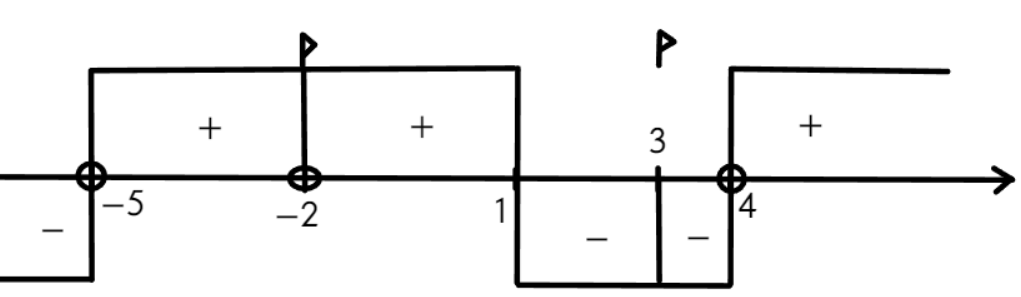
\includegraphics[scale=0.35]{ner9-1.png}}
\end{figure}\\
2. $\cfrac{(x^2-8x+15)(x-5)(x^2-2x+3)}{(x^2-3x-18)(x+1)^2}\geqslant0\Leftrightarrow\cfrac{(x-3)(x-5)^2((x-1)^2+2)}{(x-6)(x+3)(x+1)^2}\geqslant0.$ Применив метод интервалов, найдём ответ: $x\in(-3;-1)\cup(-1;3]\cup\{5\}\cup(6;+\infty).$
\begin{figure}[ht!]
\center{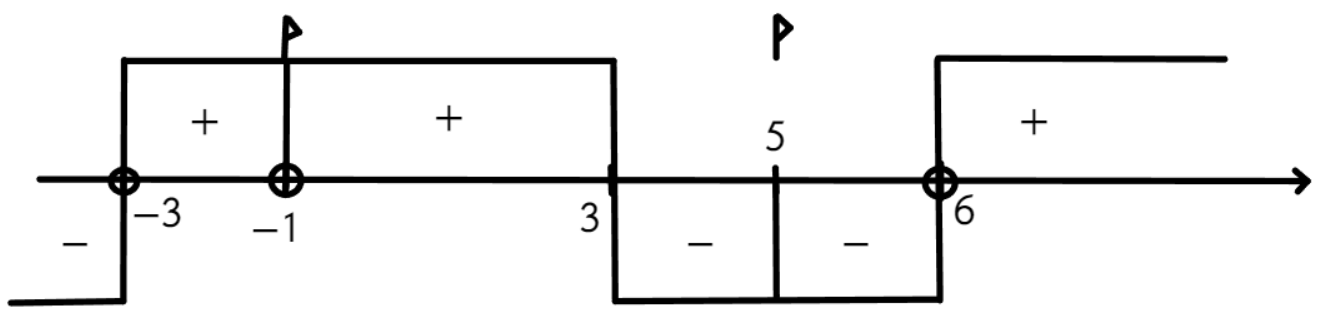
\includegraphics[scale=0.35]{ner9-2.png}}
\end{figure}\\
3. $\cfrac{x(x^2+2)(2-x)(x^3-64)}{(x^2-16)(x+2)^2}\leqslant 0 \Leftrightarrow \cfrac{x(2-x)(x-4)(x^2+4x+16)}{(x-4)(x+4)(x+2)^2}\leqslant 0.$ Применив метод интервалов, найдём ответ: $x\in(-4;-2)\cup(-2;0]\cup[2;4)\cup(4;+\infty).$
\begin{figure}[ht!]
\center{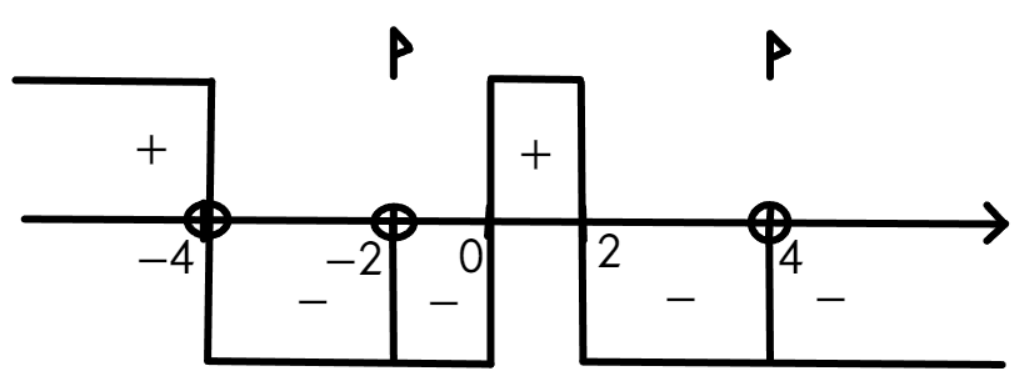
\includegraphics[scale=0.35]{ner9-3.png}}
\end{figure}\\
4. $\cfrac{x(x^2+3)(3-x)(x^3-8)}{(x^2-4)(x+3)^2}\leqslant 0 \Leftrightarrow \cfrac{x(3-x)(x-2)(x^2+2x+4)}{(x-2)(x+2)(x+3)^2}\leqslant 0.$ Применив метод интервалов, найдём ответ: $x\in(-2;0]\cup[3;+\infty).$
\begin{figure}[ht!]
\center{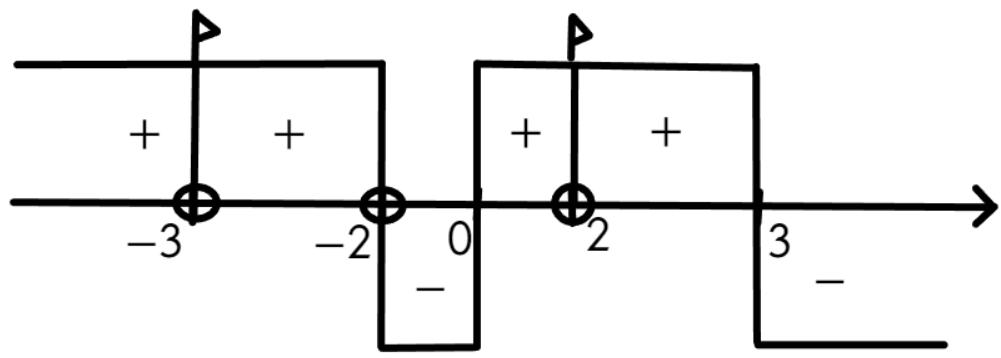
\includegraphics[scale=0.35]{ner9-4.png}}
\end{figure}\\
5. $\cfrac{x^2+3}{x+1}\leqslant2 \Leftrightarrow \cfrac{x^2+3-2x-2}{x+1} \leqslant0\Leftrightarrow \cfrac{(x-1)^2}{x+1} \leqslant0.$ Применив метод интервалов, найдём ответ: $x\in(-\infty;-1)\cup\{1\}.$\\
6. $\cfrac{x^2}{x-1}\leqslant4 \Leftrightarrow \cfrac{x^2-4x+4}{x-1}\leqslant0 \Leftrightarrow \cfrac{(x-2)^2}{x-1}\leqslant0.$ Применив метод интервалов, найдём ответ: $x\in(-\infty;1)\cup\{2\}.$\\
7. $|2x+4|<2|x|+x \Leftrightarrow \left[\begin{array}{l}\begin{cases}-2x-4<-2x+x,\\ x\leqslant-2.\end{cases}\\ \begin{cases}2x+4<-2x+x,\\ -2<x<0.\end{cases}\\ \begin{cases}2x+4<2x+x,\\ x\geqslant0.\end{cases} \end{array}\right.\Leftrightarrow \left[\begin{array}{l}\begin{cases}x>-4,\\ x\leqslant-2.\end{cases}\\ \begin{cases}x<-\cfrac{4}{3},\\ -2<x<0.\end{cases}\\ \begin{cases}x>4,\\ x\geqslant0.\end{cases} \end{array}\right.\Leftrightarrow
x\in\left(-4;-\cfrac{4}{3}\right)\cup(4;+\infty).$\\
8. $|3x+6|<3|x|+x \Leftrightarrow \left[\begin{array}{l}\begin{cases}-3x-6<-3x+x,\\ x\leqslant-2.\end{cases}\\ \begin{cases}3x+6<-3x+x,\\ -2<x<0.\end{cases}\\ \begin{cases}3x+6<3x+x,\\ x\geqslant0.\end{cases} \end{array}\right.\Leftrightarrow \left[\begin{array}{l}\begin{cases}x>-6,\\ x\leqslant-2.\end{cases}\\ \begin{cases}x<-\cfrac{6}{5},\\ -2<x<0.\end{cases}\\ \begin{cases}x>6,\\ x\geqslant0.\end{cases} \end{array}\right.\Leftrightarrow
x\in\left(-6;-\cfrac{6}{5}\right)\cup(6;+\infty).$\\
9. $\cfrac{(x-2)(x-3)}{(x-1)^2}\geqslant0.$ Применив метод интервалов, найдём ответ: $x\in(-\infty;1)\cup(1;2]\cup[3;+\infty).$
\begin{figure}[ht!]
\center{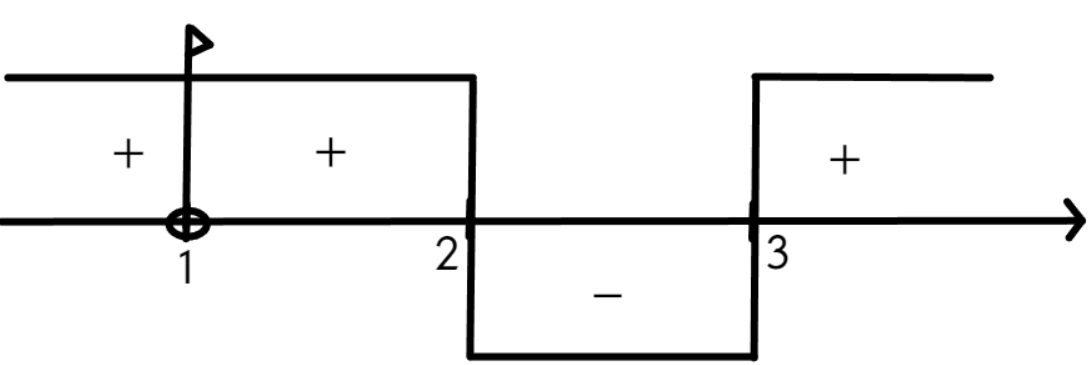
\includegraphics[scale=0.35]{ner9-9.png}}
\end{figure}\\
10. $\cfrac{(x+2)(x+3)}{(x+1)^2}\geqslant0.$ Применив метод интервалов, найдём ответ: $x\in(-\infty;-3]\cup[-2;-1)\cup(-1;+\infty).$
\begin{figure}[ht!]
\center{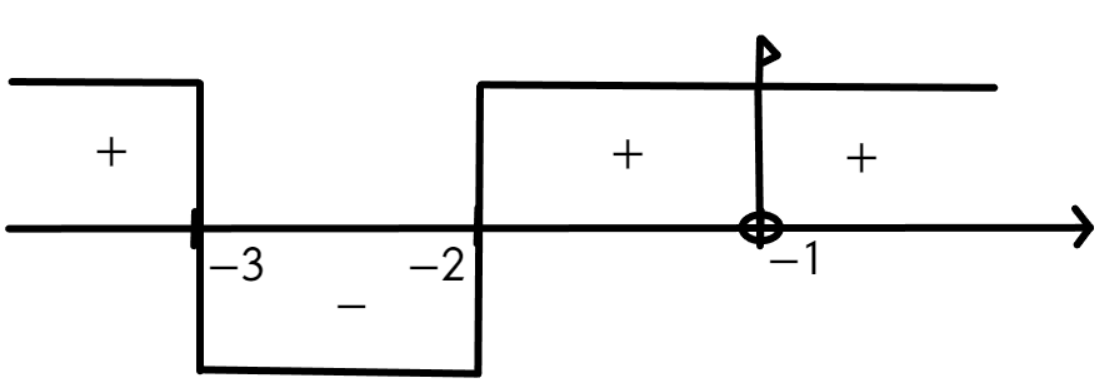
\includegraphics[scale=0.35]{ner9-10.png}}
\end{figure}\\
11. $|x^2-16|\leqslant8-2x \Leftrightarrow \begin{cases} x^2-16\leqslant8-2x,\\ x^2-16\geqslant2x-8.\end{cases} \Leftrightarrow
\begin{cases} x^2+2x-24\leqslant0,\\ x^2-2x-8\geqslant0.\end{cases}\Leftrightarrow\begin{cases} (x-4)(x+6)\leqslant0,\\ (x-4)(x+2)\geqslant0.\end{cases}
\Leftrightarrow\begin{cases} x\in[-6;4],\\ x\in(-\infty;-2]\cup[4;+\infty).\end{cases}\Leftrightarrow x\in[-6;-2]\cup\{4\}.$\\
12. $|x^2-16|\leqslant8+2x \Leftrightarrow \begin{cases} x^2-16\leqslant8+2x,\\ x^2-16\geqslant-2x-8.\end{cases} \Leftrightarrow
\begin{cases} x^2-2x-24\leqslant0,\\ x^2+2x-8\geqslant0.\end{cases}\Leftrightarrow\begin{cases} (x+4)(x-6)\leqslant0,\\ (x+4)(x-2)\geqslant0.\end{cases}
\Leftrightarrow\begin{cases} x\in[-4;6],\\ x\in(-\infty;-4]\cup[2;+\infty).\end{cases}\Leftrightarrow x\in\{-4\}\cup[2;6].$\\
13. $\cfrac{(x+1)(x+2)}{x^2+7x+12}\leqslant1 \Leftrightarrow \cfrac{x^2+2x+x+2-x^2-7x-12}{x^2+7x+12}\leqslant0 \Leftrightarrow
\cfrac{-4\left(x+\cfrac{5}{2}\right)}{(x+4)(x+3)}\leqslant0.$ Применив метод интервалов, найдём ответ: $x\in(-4;-3)\cup\left[-\cfrac{5}{2};+\infty\right)$
\begin{figure}[ht!]
\center{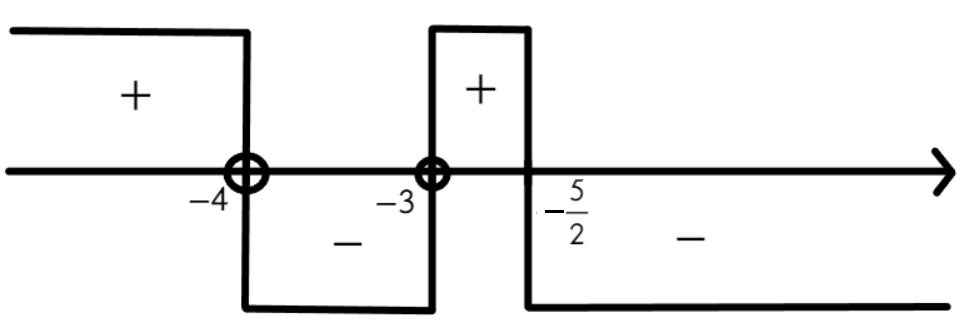
\includegraphics[scale=0.35]{ner9-13.png}}
\end{figure}\\
14. $\cfrac{x^2+3x-13}{(x+3)(x-2)}>2 \Leftrightarrow \cfrac{x^2+3x-13-2x^2+4x-6x+12}{(x+3)(x-2)}>0\Leftrightarrow \cfrac{-(x^2-x+1)}{(x+3)(x-2)}>0
\Leftrightarrow x\in(-3;2).$\\
15. $1,5x-|x|+|2x-4|\geqslant4\Leftrightarrow 1,5x+|2x-4|\geqslant |x|+4\Leftrightarrow \left[\begin{array}{l} \begin{cases} 1,5x-2x+4\geqslant -x+4,\\
x\leqslant0.\end{cases}\\ \begin{cases} 1,5x-2x+4\geqslant x+4,\\ 0<x<2.\end{cases} \\ \begin{cases} 1,5x+2x-4\geqslant x+4,\\ 2\leqslant x.\end{cases}\end{array}\right.
\Leftrightarrow \left[\begin{array}{l} \begin{cases} x\geqslant 0,\\
x\leqslant0.\end{cases}\\ \begin{cases} x\leqslant 0,\\ 0<x<2.\end{cases} \\ \begin{cases} x\geqslant \cfrac{16}{5},\\ 2\leqslant x.\end{cases}\end{array}\right.
\Leftrightarrow x\in \{0\}\cup\left[\cfrac{16}{5};+\infty\right).$\\
16. $2x-5+2|x-3|<|x+1|\Leftrightarrow \left[\begin{array}{l} \begin{cases} 2x-5-2x+6< -x-1,\\
x\leqslant-1.\end{cases}\\ \begin{cases} 2x-5-2x+6< x+1,\\ -1<x<3.\end{cases} \\ \begin{cases} 2x-5+2x-6< x+1,\\ 3\leqslant x.\end{cases}\end{array}\right.
\Leftrightarrow \left[\begin{array}{l} \begin{cases} x< -2,\\
x\leqslant-1.\end{cases}\\ \begin{cases} x> 0,\\ -1<x<3.\end{cases} \\ \begin{cases} x<4,\\ 3\leqslant x.\end{cases}\end{array}\right.
\Leftrightarrow$\\$ x\in (-\infty;-2)\cup(0;4).$\\
17. $\cfrac{2x^2+3x-13}{(x+3)(x-2)}>2\Leftrightarrow\cfrac{2x^2+3x-13-2x^2+4x-6x+12}{(x+3)(x-2)}>0\Leftrightarrow \cfrac{x-1}{(x+3)(x-2)}>0.$
Применив метод интервалов, найдём ответ: $x\in(-3;1)\cup(2;+\infty).$
\begin{figure}[ht!]
\center{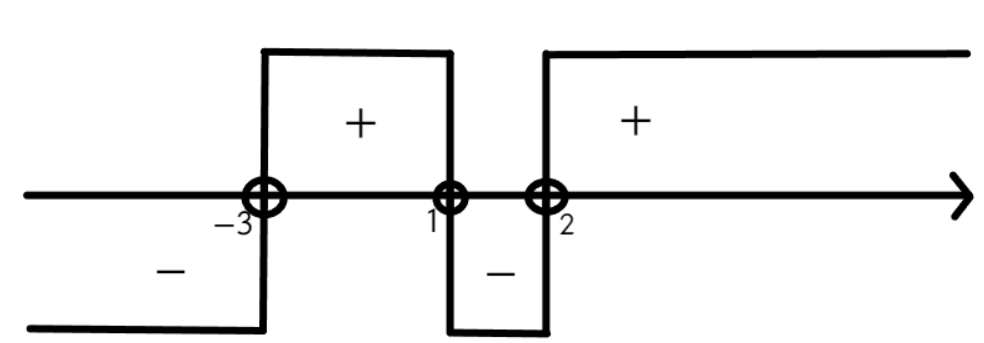
\includegraphics[scale=0.35]{ner9-17.png}}
\end{figure}\\
18. $|x^2-7x+7|>x-5\Leftrightarrow \left[\begin{array}{l} x^2-7x+7>x-5,\\ x^2-7x+7<-x+5.\end{array}\right.\Leftrightarrow
\left[\begin{array}{l} x^2-8x+12>0,\\ x^2-6x+2<0.\end{array}\right.\Leftrightarrow$\\$
\left[\begin{array}{l} (x-6)(x-2)>0,\\ (x-(3+\sqrt{7}))(x-(3-\sqrt{7}))<0.\end{array}\right.\Leftrightarrow
\left[\begin{array}{l} x\in(-\infty;2)\cup(6;+\infty),\\ x\in(3-\sqrt{7};3+\sqrt{7}).\end{array}\right.\Leftrightarrow
x\in (-\infty;3+\sqrt{7})\cup(6;+\infty).$\\
19. $|x^2-4x-14|<x+10\Leftrightarrow \begin{cases}x^2-4x-14<x+10,\\ x^2-4x-14>-x-10.\end{cases}\Leftrightarrow
\begin{cases}x^2-5x-24<0,\\ x^2-3x-4>0.\end{cases}\Leftrightarrow$\\$
\begin{cases}(x-8)(x+3)<0,\\ (x-4)(x+1)>0.\end{cases}\Leftrightarrow
\begin{cases}x\in(-3;8),\\ x\in(-\infty;-1)\cup(4;+\infty).\end{cases}\Leftrightarrow x\in (-3;-1)\cup(4;8).$\\
20. $\cfrac{(x-1)(x-2)}{x^2+7x+12}\leqslant1\Leftrightarrow \cfrac{x^2-2x-x+2-x^2-7x-12}{x^2+7x+12}\leqslant0
\Leftrightarrow \cfrac{-10(x+1)}{(x+3)(x+4)}\leqslant0.$ Применив метод интервалов, найдём ответ: $x\in(-4;-3)\cup[-1;+\infty).$
\begin{figure}[ht!]
\center{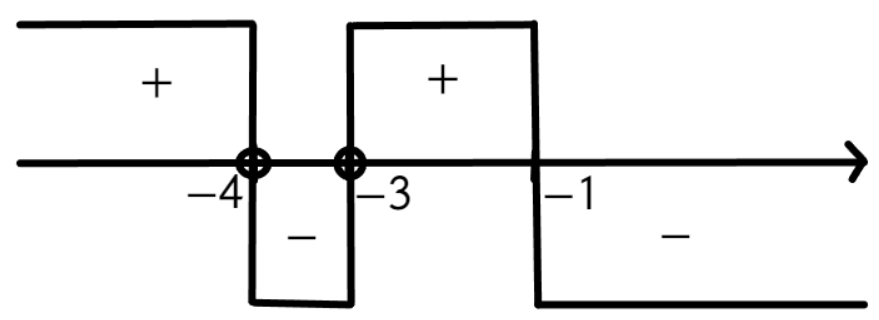
\includegraphics[scale=0.35]{ner9-20.png}}
\end{figure}\\
21. $\cfrac{(x-1)(x+3)}{x^2+7x+12}\leqslant1\Leftrightarrow \cfrac{x^2+3x-x-3-x^2-7x-12}{x^2+7x+12}\leqslant0
\Leftrightarrow \cfrac{-5(x+3)}{(x+3)(x+4)}\leqslant0\Leftrightarrow \begin{cases} x+4>0,\\ x\neq-3.\end{cases}
\Leftrightarrow x\in(-4;-3)\cup(-3;+\infty).$\\
22. $\cfrac{x^2-2x-8}{|x-4|}<7\Leftrightarrow\cfrac{(x-4)(x+2)}{|x-4|}<7\Leftrightarrow \left[\begin{array}{l} \begin{cases}x+2<7,\\ x>4.\end{cases}\\
\begin{cases}x+2>-7,\\ x<4.\end{cases}\end{array}\right.\Leftrightarrow  x\in (-9;4)\cup(4;5).$\\
23. $\cfrac{x^2-4x-5}{|x-5|}<7\Leftrightarrow\cfrac{(x-5)(x+1)}{|x-5|}<7\Leftrightarrow \left[\begin{array}{l} \begin{cases}x+1<7,\\ x>5.\end{cases}\\
\begin{cases}x+1>-7,\\ x<5.\end{cases}\end{array}\right.\Leftrightarrow  x\in (-8;5)\cup(5;6).$\\
24. $\cfrac{x^2+9x+20}{(2x-x^2-1)(3x^2+x+2)}\leqslant0\Leftrightarrow \cfrac{(x+4)(x+5)}{-(x-1)^2\left(\left(x+\cfrac{1}{2}\right)^2+2x^2+\cfrac{3}{4}\right)}\leqslant0.$ Применив метод интервалов, найдём ответ: $x\in
(-\infty;-5]\cup[-4;1)\cup(1;+\infty).$
\begin{figure}[ht!]
\center{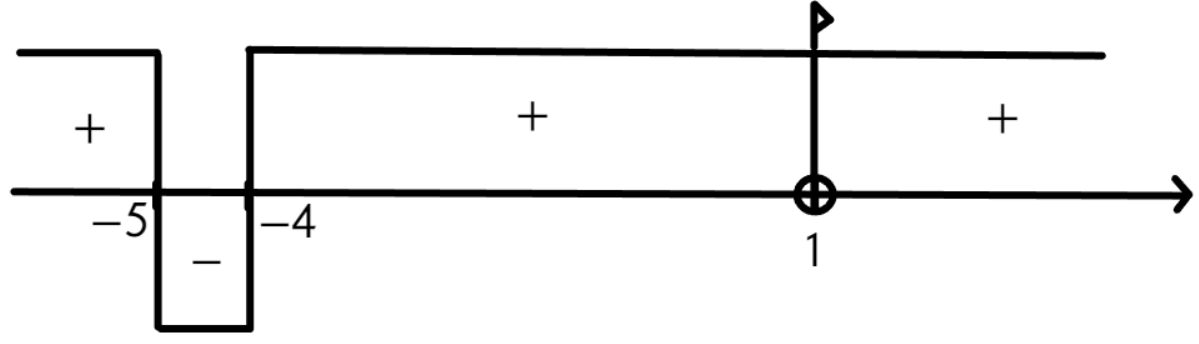
\includegraphics[scale=0.35]{ner9-24.png}}
\end{figure}\newpage\noindent
25. $\cfrac{(2x^2+x+1)(6x-x^2-9)}{x^2+8x+15}\geqslant0\Leftrightarrow \cfrac{-\left(\left(x+\cfrac{1}{2}\right)+x^2+\cfrac{3}{4}\right)(x-3)^2}{(x+3)(x+5)}\geqslant0.$ Применив метод интервалов, найдём ответ: $x\in
(-5;-3)\cup\{3\}.$
\begin{figure}[ht!]
\center{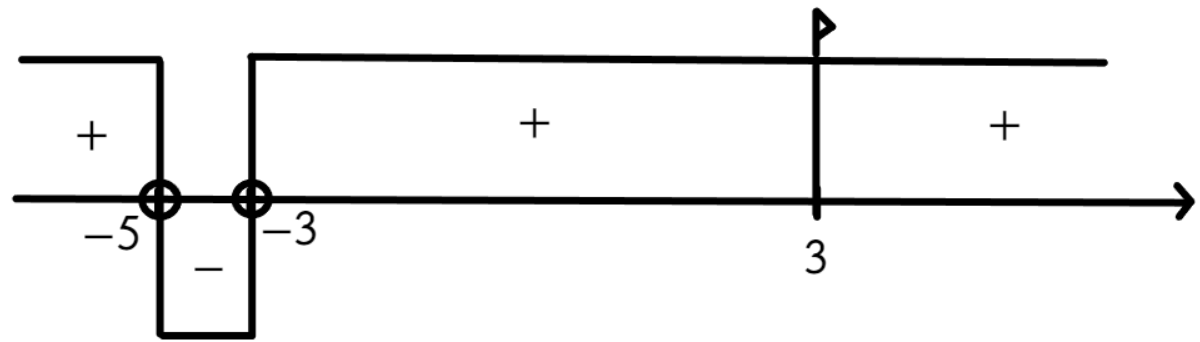
\includegraphics[scale=0.35]{ner9-25.png}}
\end{figure}\\
26. $\cfrac{(x^2-2x-8)(x^2-4x)}{x^2+7x+10}>0\Leftrightarrow\cfrac{x(x-4)^2(x+2)}{(x+2)(x+5)}>0.$ Применив метод интервалов, найдём ответ: $x\in
(-\infty;-5)\cup(0;4)\cup(4;+\infty).$
\begin{figure}[ht!]
\center{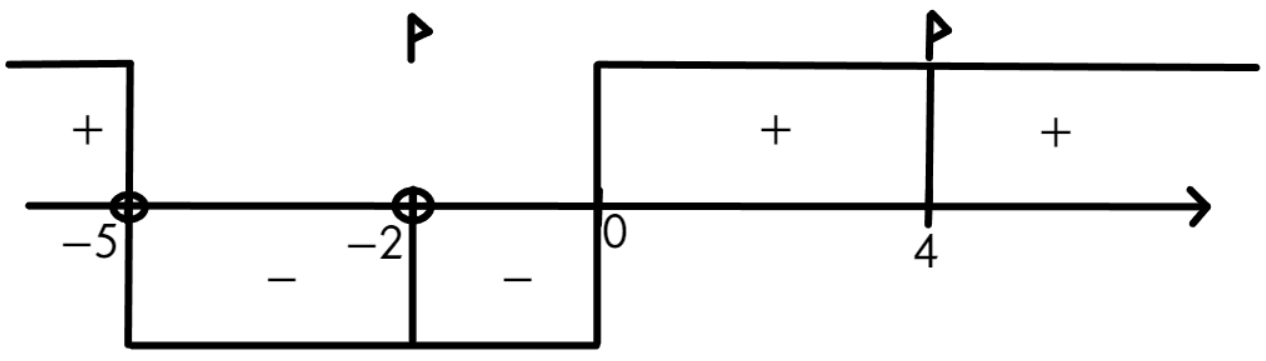
\includegraphics[scale=0.35]{ner9-26.png}}
\end{figure}\\
27. $\cfrac{(x^2-6x+8)(x^2-4)}{x^3+8}\geqslant0\Leftrightarrow \cfrac{(x-4)(x-2)^2(x+2)}{(x+2)(x^2-2x+4)}\geqslant0.$ Применив метод интервалов, найдём ответ: $x\in\{2\}\cup[4;+\infty).$
\begin{figure}[ht!]
\center{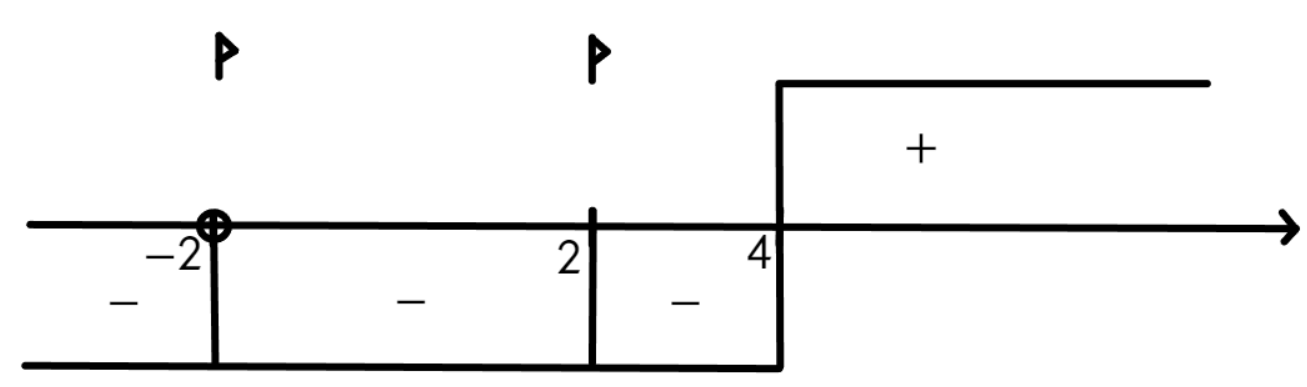
\includegraphics[scale=0.35]{ner9-27.png}}
\end{figure}\\
28. $x^2-2x-8<7|x-4|\Leftrightarrow \left[\begin{array}{l} 7x-28>x^2-2x-8,\\ 7x-28<-x^2+2x+8.\end{array}\right.\Leftrightarrow
\left[\begin{array}{l} x^2-9x-20<0,\\ x^2+5x-36<0.\end{array}\right.\Leftrightarrow$\\$
\left[\begin{array}{l} (x-5)(x-4)<0,\\ (x-4)(x+9)<0.\end{array}\right.\Leftrightarrow
\left[\begin{array}{l} x\in(4;5),\\ x\in(-9;4).\end{array}\right.\Leftrightarrow x\in (-9;4)\cup(4;5).$\\
29. $|x^2-3x|+2x-6\leqslant0\Leftrightarrow|x^2-3x|\leqslant6-2x\Leftrightarrow \begin{cases} x^2-3x\leqslant6-2x,\\ x^2-3x\geqslant2x-6.\end{cases}
\Leftrightarrow \begin{cases} x^2-x-6\leqslant0,\\ x^2-5x+6\geqslant0.\end{cases}
\Leftrightarrow \begin{cases} (x-3)(x+2)\leqslant0,\\ (x-3)(x-2)\geqslant0.\end{cases}
\Leftrightarrow \begin{cases} x\in[-2;3],\\ x\in(-\infty;2]\cup[3;+\infty).\end{cases}\Leftrightarrow x \in [-2;2]\cup\{3\}.$\newpage\noindent
30. $\cfrac{(x^2-4x+4)(9-x^2)}{x^2+8x+16}\leqslant0\Leftrightarrow\cfrac{-(x-2)^2(x-3)(x+3)}{(x+4)^2}\leqslant0.$ Применив метод интервалов, найдём ответ: $x\in
(-\infty;-4)\cup(-4;-3]\cup\{2\}\cup[3;+\infty).$
\begin{figure}[ht!]
\center{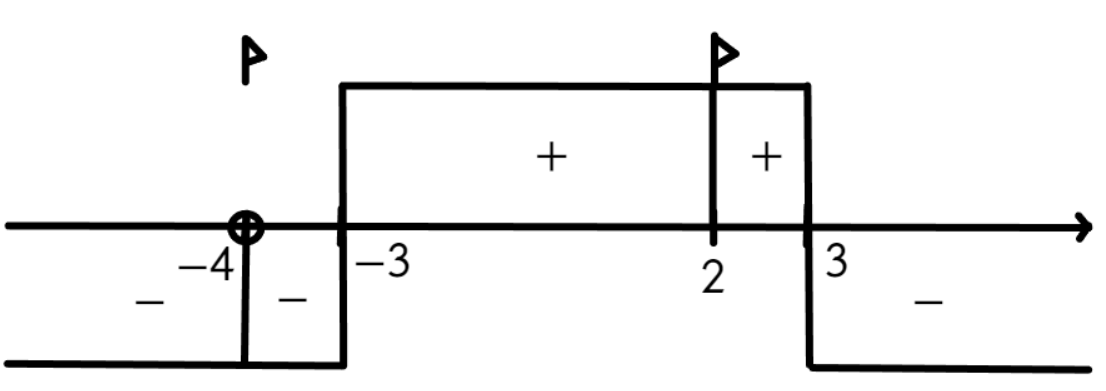
\includegraphics[scale=0.35]{ner9-30.png}}
\end{figure}\\
31. $\cfrac{(x^2+14x+49)(16-x^2)}{x^2-6x+9}\geqslant0\Leftrightarrow\cfrac{-(x+7)^2(x-4)(x+4)}{(x-3)^2}\geqslant0.$ Применив метод интервалов, найдём ответ: $x\in
\{-7\}\cup[-4;3)\cup(3;4].$
\begin{figure}[ht!]
\center{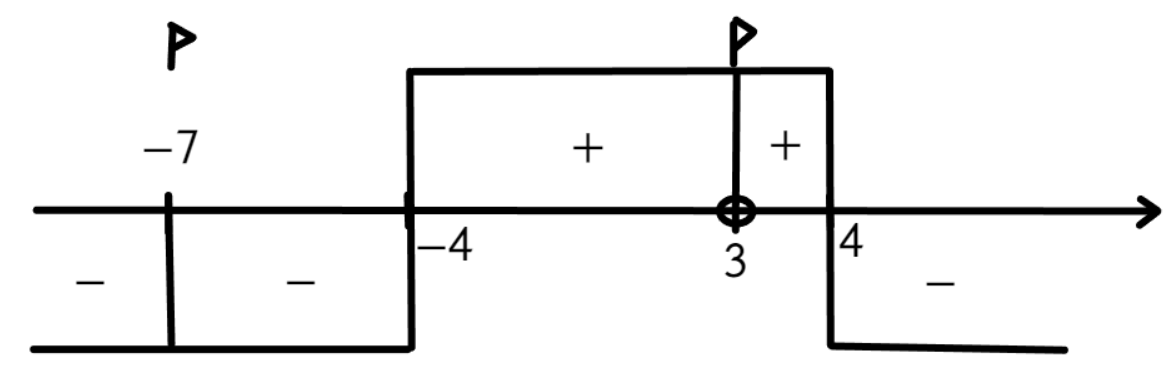
\includegraphics[scale=0.35]{ner9-31.png}}
\end{figure}\\
32. $\cfrac{(1-x^2)(x-1)^2(x+1)^3}{x^6+x^4+x^2}\leqslant0\Leftrightarrow\cfrac{-(x-1)^3(x+1)^4}{x^2(x^4+x^2+1)}\leqslant0.$ Применив метод интервалов, найдём ответ: $x\in\{-1\}\cup[1;+\infty).$
\begin{figure}[ht!]
\center{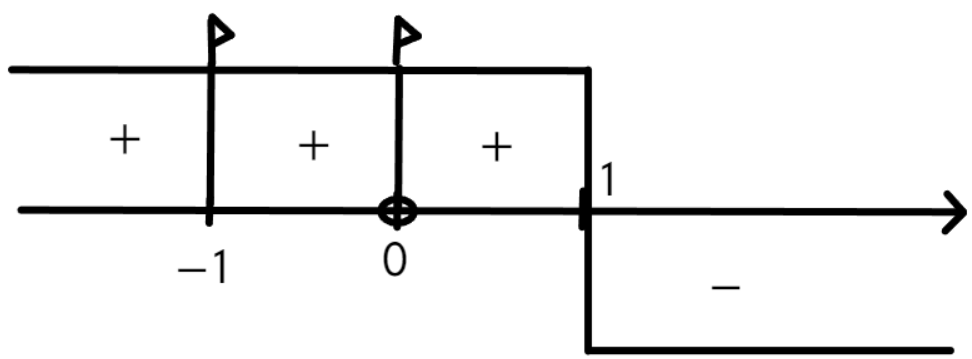
\includegraphics[scale=0.35]{ner9-32.png}}
\end{figure}\\
33. $\cfrac{(-1+x^2)(1-x)^2(x+1)^3}{x^8-x^6+x^4}\leqslant0\Leftrightarrow\cfrac{(x-1)^3(x+1)^4}{x^4(x^4-x^2+1)}\leqslant0.$ Применив метод интервалов, найдём ответ: $x\in(-\infty;0)\cup(0;1].$
\begin{figure}[ht!]
\center{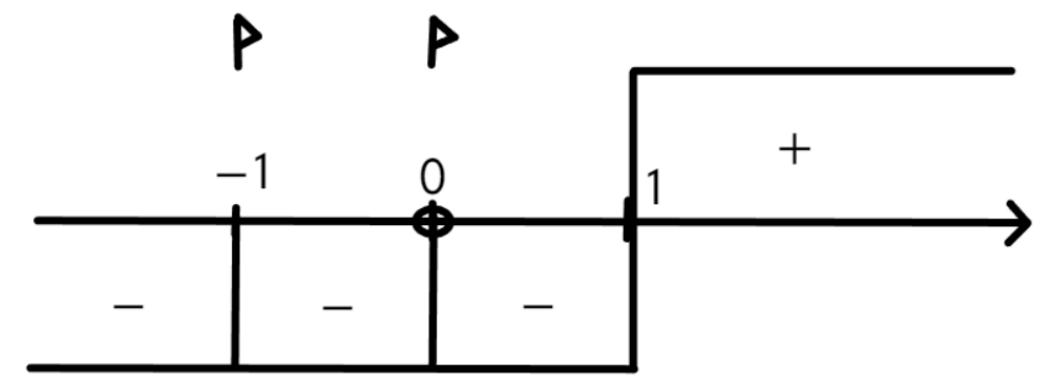
\includegraphics[scale=0.35]{ner9-33.png}}
\end{figure}\\
34. $\left|\cfrac{x-1}{x+2}\right|>1\Leftrightarrow \left[\begin{array}{l} \cfrac{x-1}{x+2}>1,\\ \cfrac{x-1}{x+2}<-1.\end{array}\right.\Leftrightarrow
\left[\begin{array}{l} \cfrac{x-1-x-2}{x+2}>0,\\ \cfrac{x-1+x+2}{x+2}<0.\end{array}\right.\Leftrightarrow
\left[\begin{array}{l} \cfrac{-3}{x+2}>0,\\ \cfrac{2x+1}{x+2}<0.\end{array}\right.\Leftrightarrow
\left[\begin{array}{l} x<-2,\\ -2<x<-\cfrac{1}{2}.\end{array}\right.\Leftrightarrow$\\$
 x\in (-\infty;-2)\cup\left(-2;-\cfrac{1}{2}\right).$\\
35. $\left|\cfrac{x+2}{x-1}\right|<1\Leftrightarrow \begin{cases} \cfrac{x+2}{x-1}<1,\\ \cfrac{x+2}{x-1}>-1.\end{cases}\Leftrightarrow
\begin{cases} \cfrac{x+2-x+1}{x-1}<0,\\ \cfrac{x+2+x-1}{x-1}>0.\end{cases}\Leftrightarrow
\begin{cases} \cfrac{3}{x-1}<0,\\ \cfrac{2x+1}{x-1}>0.\end{cases}\Leftrightarrow$\\$
\begin{cases} x<1,\\ x\in\left(-\infty;-\cfrac{1}{2}\right)\cup(1;+\infty).\end{cases}\Leftrightarrow
 x\in \left(-\infty;-\cfrac{1}{2}\right).$\\
36. $\cfrac{(x+1)\sqrt{-x^2-10x+11}}{x^2+x-12}\geqslant0\Leftrightarrow \cfrac{(x+1)\sqrt{-(x+11)(x-1)}}{(x+4)(x-3)}\geqslant0.$ Применив метод интервалов, найдём ответ: $x\in\{-11;1\}\cup(-4;-1].$
\begin{figure}[ht!]
\center{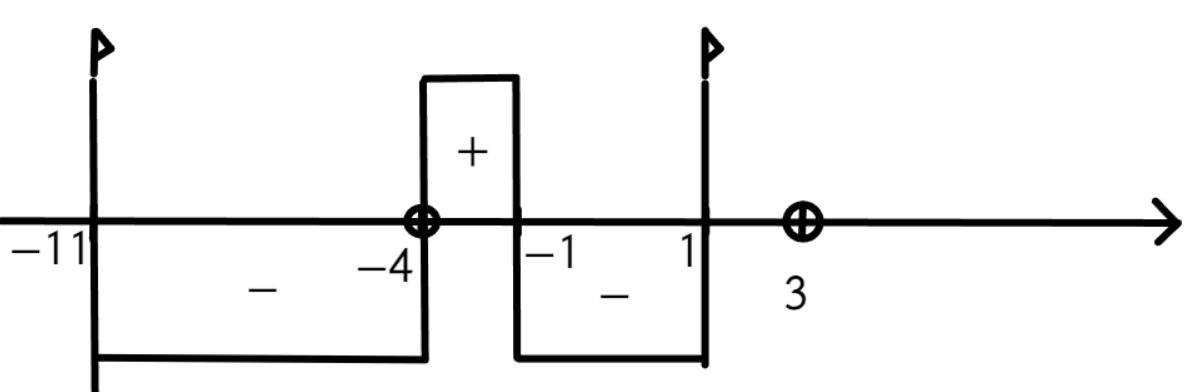
\includegraphics[scale=0.35]{ner9-36.png}}
\end{figure}\\
37. $\cfrac{(x+2)\sqrt{-x^2-10x+11}}{x^2+x-12}\geqslant0\Leftrightarrow\cfrac{(x+2)\sqrt{-(x+11)(x-1)}}{(x+4)(x-3)}\geqslant0.$ Применив метод интервалов, найдём ответ: $x\in\{-11;1\}\cup(-4;-2].$
\begin{figure}[ht!]
\center{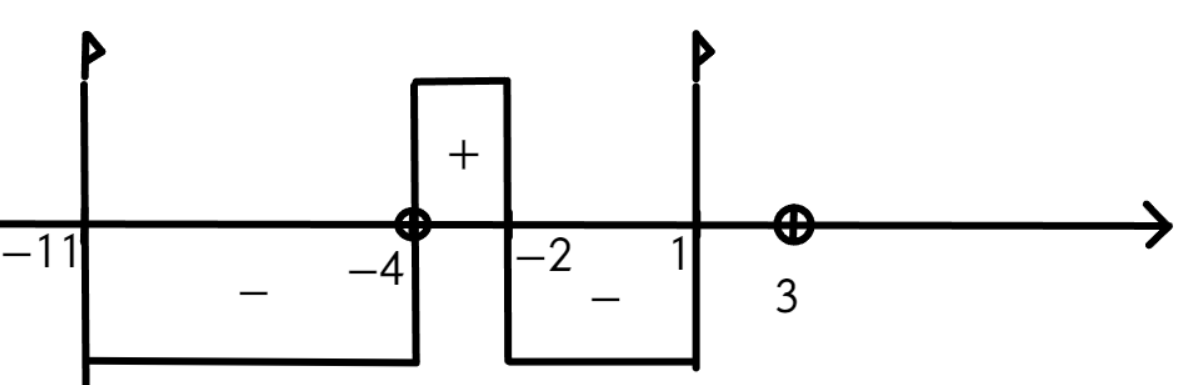
\includegraphics[scale=0.35]{ner9-37.png}}
\end{figure}\\
38. $\cfrac{4}{\sqrt{x-5}+3}>\cfrac{3}{\sqrt{x-5}+4}.$ У левой дроби больше числитель и меньше знаменатель, значит неравенство верно на всей ОДЗ, то есть $x\in[5;+\infty).$\\
39. $\cfrac{3}{\sqrt{x-4}+2}>\cfrac{2}{\sqrt{x-4}+3}.$ У левой дроби больше числитель и меньше знаменатель, значит неравенство верно на всей ОДЗ, то есть $x\in[4;+\infty).$\\
40. $\cfrac{x^2-4x+3}{2x-3}\leqslant\cfrac{x^2-4x+3}{x-2}\Leftrightarrow (x^2-4x+3)\left(\cfrac{1}{2x-3}-\cfrac{1}{x-2}\right)\leqslant0
\Leftrightarrow (x^2-4x+3)\cdot\cfrac{x-2-2x+3}{(2x-3)(x-2)}\leqslant0\Leftrightarrow\cfrac{-(x-3)(x-1)^2}{(2x-3)(x-2)}\leqslant0.$ Применив метод интервалов, найдём ответ: $x\in\{1\}\cup\left(\cfrac{3}{2};2\right)\cup[3;+\infty).$
\begin{figure}[ht!]
\center{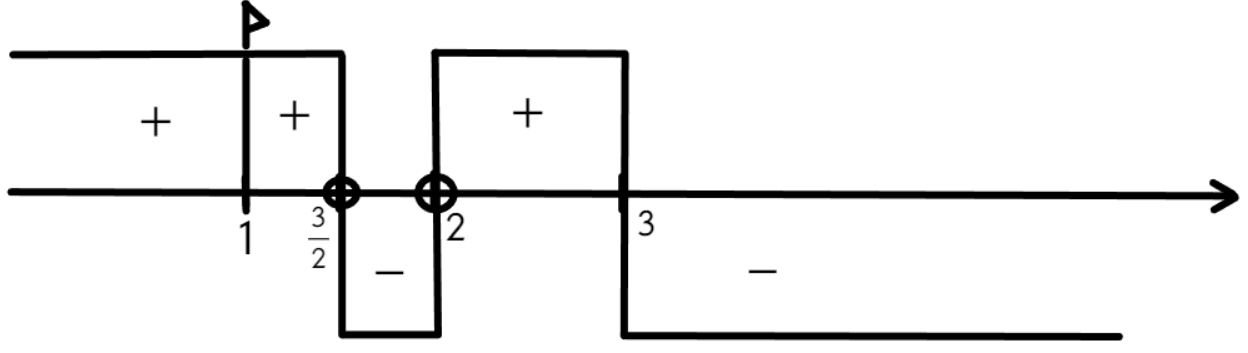
\includegraphics[scale=0.35]{ner9-40.png}}
\end{figure}\newpage\noindent
41. $\cfrac{x^2-3x+2}{2x+3}\leqslant\cfrac{x^2-3x+2}{x+5}\Leftrightarrow (x^2-3x+2)\left(\cfrac{1}{2x+3}-\cfrac{1}{x+5}\right)\leqslant0
\Leftrightarrow (x^2-3x+2)\cdot\cfrac{x+5-2x-3}{(2x+3)(x+5)}\leqslant0\Leftrightarrow\cfrac{-(x-1)(x-2)^2}{(2x+3)(x+5)}\leqslant0.$ Применив метод интервалов, найдём ответ: $x\in\left(-5;-\cfrac{3}{2}\right)\cup[1;+\infty).$
\begin{figure}[ht!]
\center{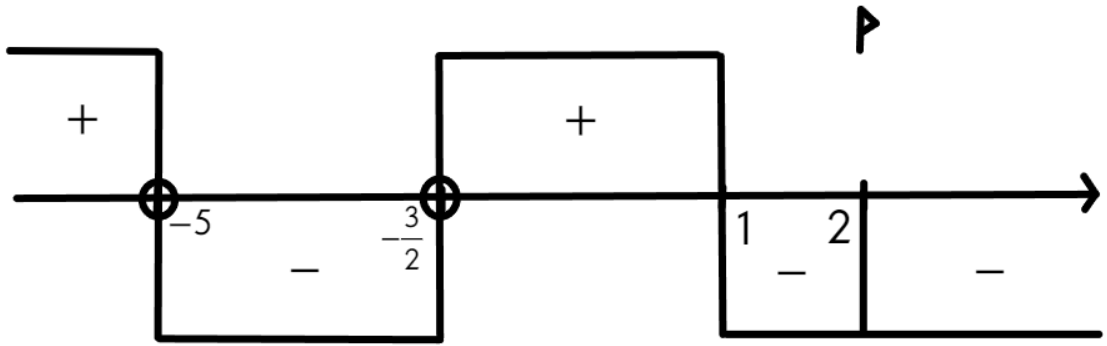
\includegraphics[scale=0.35]{ner9-41.png}}
\end{figure}\\
42. $\cfrac{(x+3)^2(x^2+4x-5)}{x^2-8x+16}\geqslant0\Leftrightarrow\cfrac{(x+3)^2(x+5)(x-1)}{(x-4)^2}\geqslant0.$ Применив метод интервалов, найдём ответ: $x\in(-\infty;-5]\cup\{-3\}\cup[1;4)\cup(4;+\infty).$
\begin{figure}[ht!]
\center{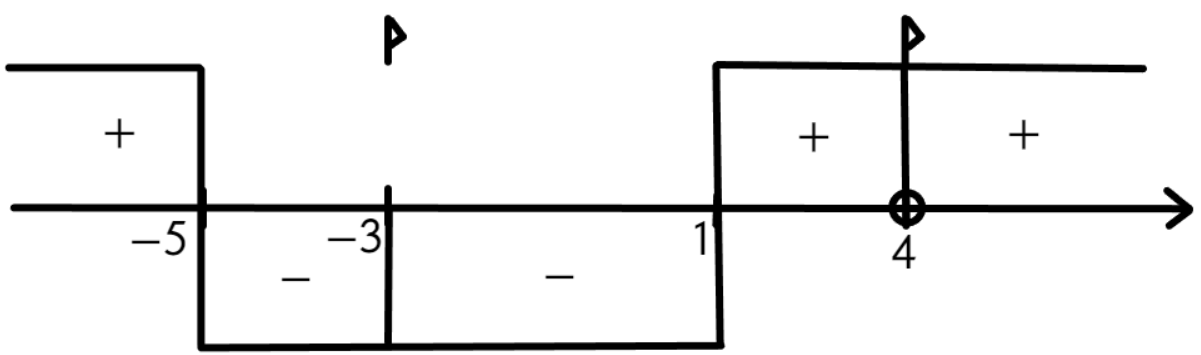
\includegraphics[scale=0.35]{ner9-42.png}}
\end{figure}\\
43. $\cfrac{(x-3)^2(x^2-3x-10)}{x^2+8x+16}\leqslant0\Leftrightarrow\cfrac{(x-3)^2(x-5)(x+2)}{(x+4)^2}\leqslant0.$ Применив метод интервалов, найдём ответ: $x\in[-2;5].$
\begin{figure}[ht!]
\center{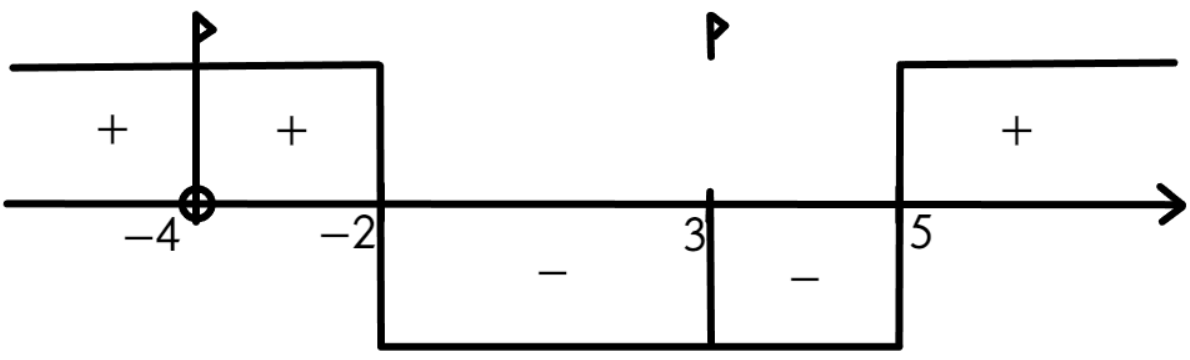
\includegraphics[scale=0.35]{ner9-43.png}}
\end{figure}\\
44. $\cfrac{(2x^2-7x+6)(x^2+3x-10)}{(x+1)(5+4x-x^2)}\leqslant0\Leftrightarrow\cfrac{(x-2)^2(x+5)(2x-3)}{-(x+1)^2(x-5)}\leqslant0.$ Применив метод интервалов, найдём ответ: $x\in[-5;-1)\cup\left(-1;\cfrac{3}{2}\right]\cup\{2\}\cup(5;+\infty).$
\begin{figure}[ht!]
\center{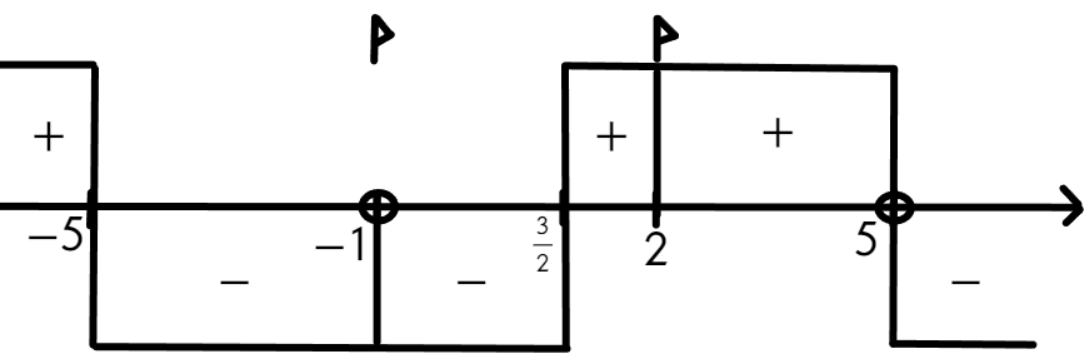
\includegraphics[scale=0.35]{ner9-44.png}}
\end{figure}\newpage\noindent
45. $\cfrac{(3x^2-5x+2)(x^2+3x-4)}{(x+2)(8+2x-x^2)}\leqslant0\Leftrightarrow\cfrac{(x-1)^2(x+4)(3x-2)}{-(x+2)^2(x-4)}\leqslant0.$ Применив метод интервалов, найдём ответ: $x\in[-4;-2)\cup\left(-2;\cfrac{2}{3}\right]\cup\{1\}\cup(4;+\infty).$
\begin{figure}[ht!]
\center{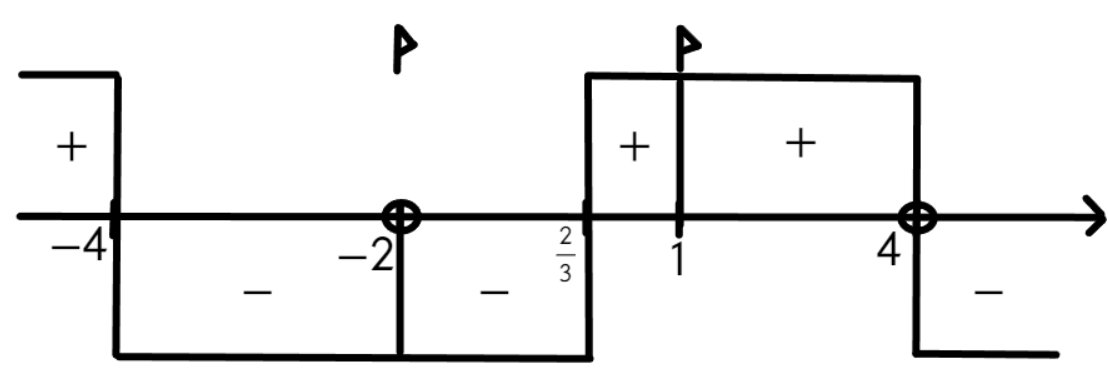
\includegraphics[scale=0.35]{ner9-45.png}}
\end{figure}\\
46. $|x-2|>2+x-|3-x|\Leftrightarrow |x-2|+|x-3|>x+2\Leftrightarrow\left[\begin{array}{l} \begin{cases} 2-x-x+3>x+2,\\
x\leqslant2.\end{cases}\\ \begin{cases} x-2-x+3>x+2,\\ 2<x<3.\end{cases} \\ \begin{cases} x-2+x-3>x+2,\\ 3\leqslant x.\end{cases}\end{array}\right.\Leftrightarrow
\left[\begin{array}{l} \begin{cases} x<1,\\
x\leqslant2.\end{cases}\\ \begin{cases} x<-1,\\ 2<x<3.\end{cases} \\ \begin{cases} x>7,\\ 3\leqslant x.\end{cases}\end{array}\right.\Leftrightarrow
x\in(-\infty;1)\cup(7;+\infty).$\\
47. $|2x+3|>|x|-4x-1\Leftrightarrow\left[\begin{array}{l} \begin{cases} -2x-3>-x-4x-1,\\
x\leqslant-\cfrac{3}{2}.\end{cases}\\ \begin{cases} 2x+3>-x-4x-1,\\ -\cfrac{3}{2}<x<0.\end{cases} \\ \begin{cases} 2x+3>x-4x-1,\\ 0\leqslant x.\end{cases}\end{array}\right.\Leftrightarrow
\left[\begin{array}{l} \begin{cases} x>\cfrac{2}{3},\\
x\leqslant-\cfrac{3}{2}.\end{cases}\\ \begin{cases} x>-\cfrac{4}{7},\\ -\cfrac{3}{2}<x<0.\end{cases} \\ \begin{cases} x>-\cfrac{4}{5},\\ 0\leqslant x.\end{cases}\end{array}\right.\Leftrightarrow$\\$
x\in\left(-\cfrac{4}{7};+\infty\right).$\\
48. $\cfrac{\sqrt{(2-x)^2}}{x-3}>2\Leftrightarrow\cfrac{|x-2|}{x-3}>2\Leftrightarrow\left[\begin{array}{l} \begin{cases} \cfrac{2-x}{x-3}>2,\\
x\leqslant2.\end{cases}\\ \begin{cases} \cfrac{x-2}{x-3}>2,\\ 2<x.\end{cases}\end{array}\right.\Leftrightarrow\left[\begin{array}{l} \begin{cases} \cfrac{2-x-2x+6}{x-3}>0,\\ x\leqslant2.\end{cases}\\ \begin{cases} \cfrac{x-2-2x+6}{x-3}>0,\\ 2<x.\end{cases}\end{array}\right.\Leftrightarrow$\\$\left[\begin{array}{l} \begin{cases} \cfrac{8-3x}{x-3}>0,\\ x\leqslant2.\end{cases}\\ \begin{cases} \cfrac{4-x}{x-3}>0,\\ 2<x.\end{cases}\end{array}\right.\Leftrightarrow\left[\begin{array}{l} \begin{cases} x\in\left(\cfrac{8}{3};3\right),\\ x\leqslant2.\end{cases}\\ \begin{cases} x\in(3;4),\\ 2<x.\end{cases}\end{array}\right.\Leftrightarrow x\in (3;4).$\\
49. $\cfrac{\sqrt{(1-x)^2}}{x-2}>3\Leftrightarrow\cfrac{|x-1|}{x-2}>3\Leftrightarrow\left[\begin{array}{l} \begin{cases} \cfrac{1-x}{x-2}>3,\\
x\leqslant1.\end{cases}\\ \begin{cases} \cfrac{x-1}{x-2}>3,\\ 1<x.\end{cases}\end{array}\right.\Leftrightarrow\left[\begin{array}{l} \begin{cases} \cfrac{1-x-3x+6}{x-2}>0,\\ x\leqslant1.\end{cases}\\ \begin{cases} \cfrac{x-1-3x+6}{x-2}>0,\\ 1<x.\end{cases}\end{array}\right.$\\$\Leftrightarrow\left[\begin{array}{l} \begin{cases} \cfrac{7-4x}{x-2}>0,\\ x\leqslant1.\end{cases}\\ \begin{cases} \cfrac{5-2x}{x-2}>0,\\ 1<x.\end{cases}\end{array}\right.\Leftrightarrow\left[\begin{array}{l} \begin{cases} x\in\left(\cfrac{7}{4};2\right),\\ x\leqslant1.\end{cases}\\ \begin{cases} x\in\left(2;\cfrac{5}{2}\right),\\ 1<x.\end{cases}\end{array}\right.\Leftrightarrow x\in\left(2;\cfrac{5}{2}\right)$\\
50. $\cfrac{2x^2-15x+7}{\sqrt{14+5x-x^2}}\geqslant0\Leftrightarrow\cfrac{(2x-1)(x-7)}{\sqrt{-(x+2)(x-7)}}\geqslant0.$ Применив метод интервалов, найдём ответ:\\ $x\in\left(-2;\cfrac{1}{2}\right].$
\begin{figure}[ht!]
\center{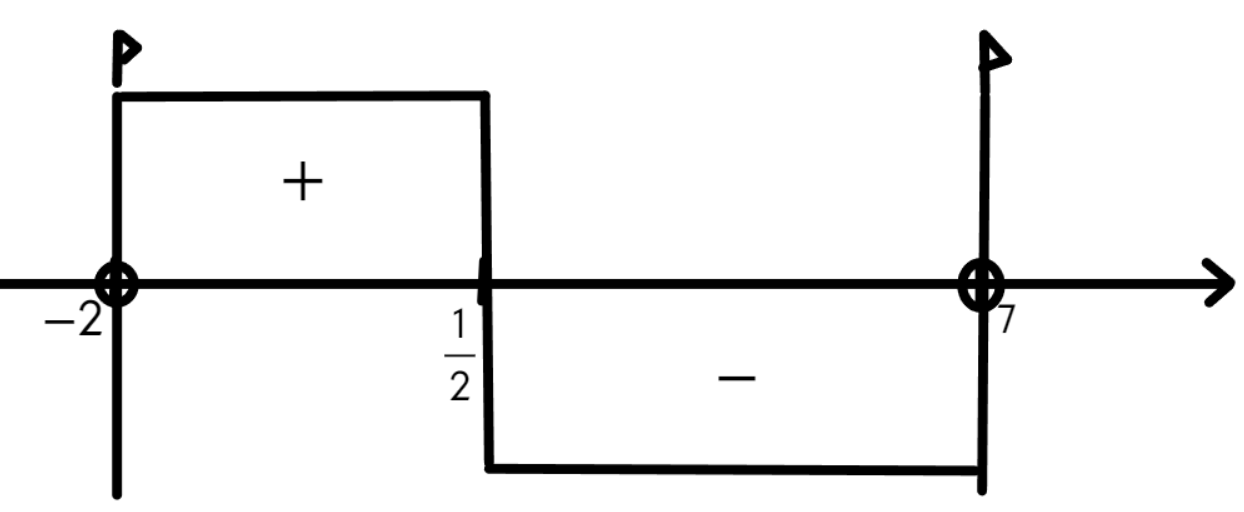
\includegraphics[scale=0.35]{ner9-50.png}}
\end{figure}\\
51. $\cfrac{3x^2-19x+6}{\sqrt{18+3x-x^2}}\geqslant0\Leftrightarrow\cfrac{(3x-1)(x-6)}{\sqrt{-(x+3)(x-6)}}\geqslant0.$ Применив метод интервалов, найдём ответ:\\ $x\in\left(-3;\cfrac{1}{3}\right].$
\begin{figure}[ht!]
\center{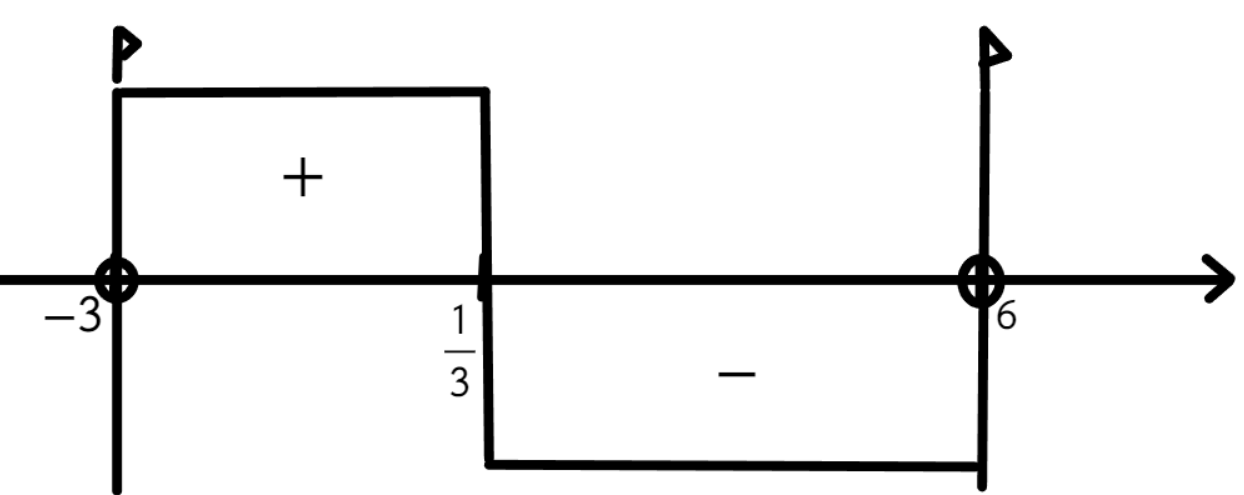
\includegraphics[scale=0.35]{ner9-51.png}}
\end{figure}\newpage\noindent
52. $\cfrac{|x-2|(3x^2+2x-1)}{4+3x-x^2}\leqslant0\Leftrightarrow\cfrac{|x-2|(3x-1)(x+1)}{-(x+1)(x-4)}\leqslant0.$ Применив метод интервалов, найдём ответ: $x\in(-\infty;-1)\cup\left(-1;\cfrac{1}{3}\right]\cup\{2\}\cup(4;+\infty).$
\begin{figure}[ht!]
\center{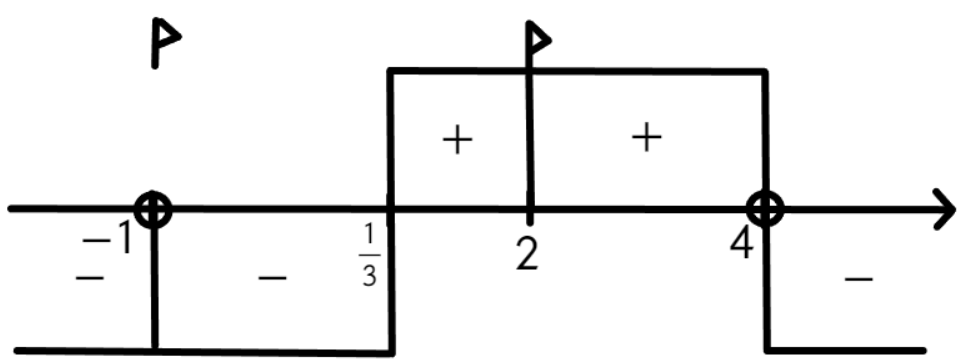
\includegraphics[scale=0.35]{ner9-52.png}}
\end{figure}\\
53. $\cfrac{|x-3|(4x^2+7x-2)}{10+3x-x^2}\leqslant0\Leftrightarrow\cfrac{|x-3|(4x-1)(x+2)}{-(x+2)(x-5)}\leqslant0.$ Применив метод интервалов, найдём ответ: $x\in(-\infty;-2)\cup\left(-2;\cfrac{1}{4}\right]\cup\{3\}\cup(5;+\infty).$
\begin{figure}[ht!]
\center{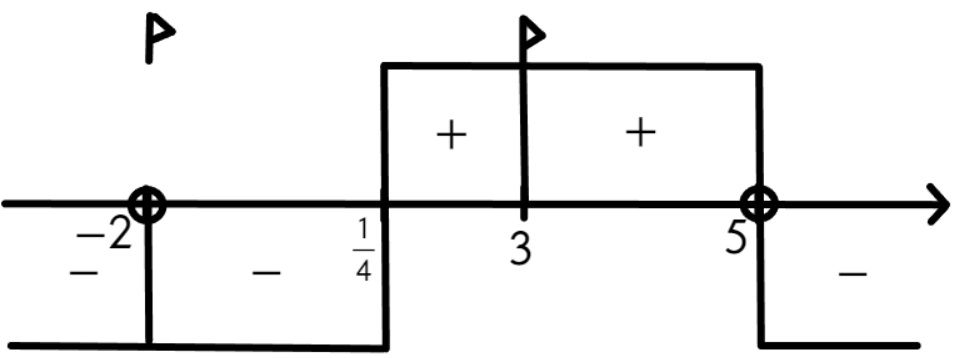
\includegraphics[scale=0.35]{ner9-53.png}}
\end{figure}\\
54. $-\cfrac{1}{2}x^2+2,5x-3\geqslant0\Leftrightarrow x^2-5x+6\leqslant0\Leftrightarrow (x-2)(x-3)\leqslant0\Leftrightarrow x\in[2;3].$\\
55. $\cfrac{4}{x^2-x-6}\geqslant(2+x)^{-1}\Leftrightarrow\cfrac{4}{(x-3)(x+2)}-\cfrac{1}{x+2}\geqslant0\Leftrightarrow\cfrac{4-x+3}{(x-3)(x+2)}\geqslant0
\Leftrightarrow\cfrac{7-x}{(x-3)(x+2)}\geqslant0.$ Применив метод интервалов, найдём ответ: $x\in(-\infty;-2)\cup(3;7].$
\begin{figure}[ht!]
\center{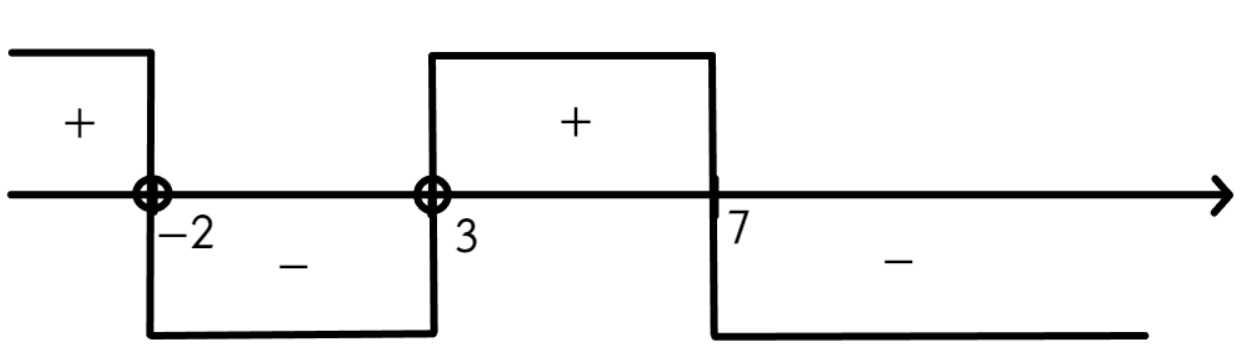
\includegraphics[scale=0.35]{ner9-55.png}}
\end{figure}\\
56. $(\sqrt{5}-3)(x^{0,5}-2x^{0,25}+1)>14-6\sqrt{5}\Leftrightarrow[t=x^{0,25}\geqslant0](\sqrt{5}-3)(t-1)^2>(\sqrt{5}-3)^2\Leftrightarrow$\\$ (t-1)^2<\sqrt{5}-3
\Leftrightarrow x\in\{\varnothing\}.$\\
57. $\cfrac{x^2-2x-8}{|x-4|}\leqslant 7\Leftrightarrow\cfrac{(x-4)(x+2)}{|x-4|}\leqslant 7\Leftrightarrow\left[\begin{array}{l} \begin{cases} x+2\leqslant7,\\ x>4.\end{cases}\\ \begin{cases} -x-2\leqslant7,\\ x<4.\end{cases}\end{array}\right.\Leftrightarrow\left[\begin{array}{l} \begin{cases} x\leqslant5,\\ x>4.\end{cases}\\ \begin{cases} x\geqslant-9,\\ x<4.\end{cases}\end{array}\right.\Leftrightarrow$\\$ x \in[-9;4)\cup(4;5].$\\
58. $|x^2-4|\leqslant3x\Leftrightarrow \begin{cases} x^2-4\leqslant3x,\\ x^2-4\geqslant-3x.\end{cases}\Leftrightarrow \begin{cases} x^2-3x-4\leqslant0,\\ x^2+3x-4\geqslant0.\end{cases}\Leftrightarrow \begin{cases} (x-4)(x+1)\leqslant0,\\ (x+4)(x-1)\geqslant0.\end{cases}
\Leftrightarrow$\\$ \begin{cases} x\in[-1;4],\\ x\in(-\infty;-4]\cup[1;+\infty).\end{cases}\Leftrightarrow x\in[1;4].$\\
59. $|x^2-9|\leqslant8x\Leftrightarrow \begin{cases} x^2-9\leqslant8x,\\ x^2-9\geqslant-8x.\end{cases}\Leftrightarrow \begin{cases} x^2-8x-9\leqslant0,\\ x^2+8x-9\geqslant0.\end{cases}\Leftrightarrow \begin{cases} (x-9)(x+1)\leqslant0,\\ (x+9)(x-1)\geqslant0.\end{cases}
\Leftrightarrow$\\$ \begin{cases} x\in[-1;9],\\ x\in(-\infty;-9]\cup[1;+\infty).\end{cases}\Leftrightarrow x\in[1;9].$\\
60. $\cfrac{x^3}{2x-1}\leqslant x\Leftrightarrow\cfrac{x^3}{2x-1}-x\leqslant0\Leftrightarrow \cfrac{x^3-2x^2+x}{2x-1}\leqslant0\Leftrightarrow
\cfrac{x(x-1)^2}{2x-1}\leqslant0.$ Применив метод интервалов, найдём ответ: $x\in\left[0;\cfrac{1}{2}\right)\cup\{1\}.$
\begin{figure}[ht!]
\center{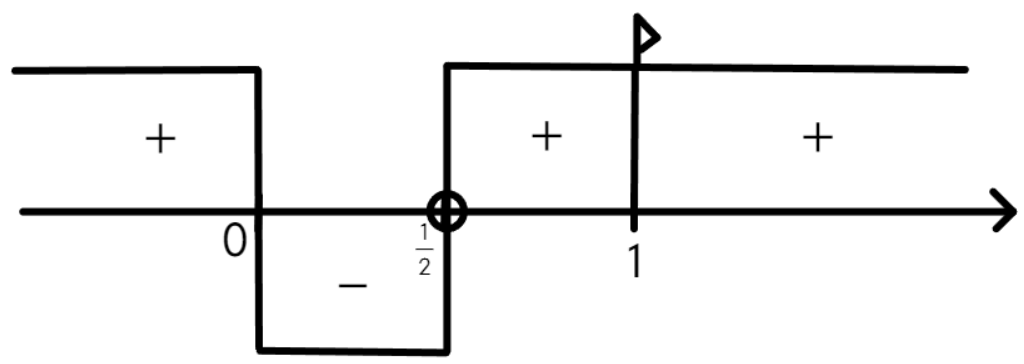
\includegraphics[scale=0.35]{ner9-60.png}}
\end{figure}\\
61. $\cfrac{(x-1)^3}{2x-3}\leqslant x-1\Leftrightarrow (x-1)\left(\cfrac{(x-1)^2}{2x-3}-1\right)\leqslant0\Leftrightarrow
(x-1)\left(\cfrac{x^2-2x+1-2x+3}{2x-3}\right)\leqslant0\Leftrightarrow\cfrac{(x-1)(x-2)^2}{2x-3}\leqslant0.$ Применив метод интервалов, найдём ответ: $x\in\left[1;\cfrac{3}{2}\right)\cup\{2\}.$
\begin{figure}[ht!]
\center{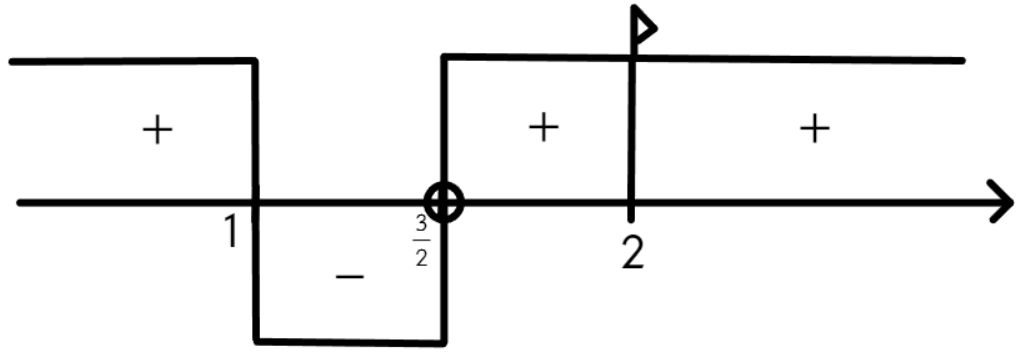
\includegraphics[scale=0.35]{ner9-61.png}}
\end{figure}\\
62. $\cfrac{x}{x+1}-\cfrac{2x}{x^2-x+1}\geqslant\cfrac{x-2x^2}{x^3+1}\Leftrightarrow \cfrac{x^3-x^2+x-2x^2-2x-x+2x^2}{(x+1)(x^2-x+1)}\geqslant0
\Leftrightarrow \cfrac{x(x+1)(x-2)}{(x+1)(x^2-x+1)}\geqslant0.$ Применив метод интервалов, найдём ответ: $x\in (-\infty;-1)\cup(-1;0]\cup[2;+\infty).$
\begin{figure}[ht!]
\center{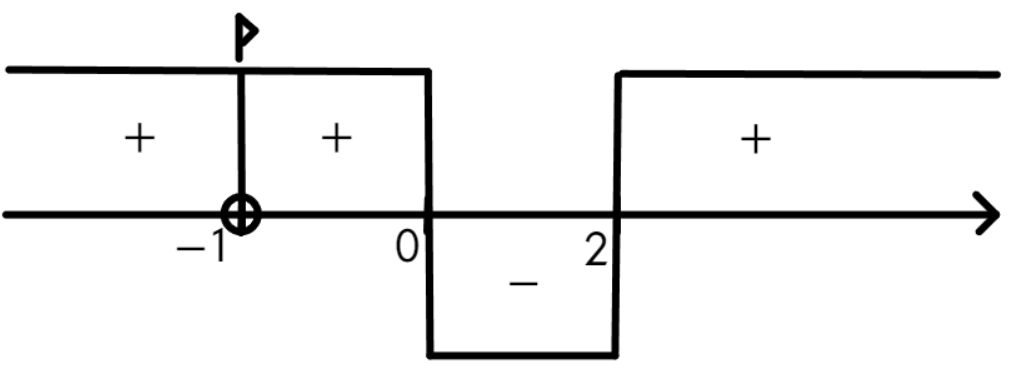
\includegraphics[scale=0.35]{ner9-62.png}}
\end{figure}\\
63. $\cfrac{2-x}{x^3+x^2}\geqslant\cfrac{1-2x}{x^3-3x^2}\Leftrightarrow\cfrac{2-x}{x^2(x+1)}+\cfrac{2x-1}{x^2(x-3)}\geqslant0\Leftrightarrow
\cfrac{2x-x^2-6+3x+2x^2-x+2x-1}{x^2(x-3)(x+1)}\geqslant0\Leftrightarrow\cfrac{(x+7)(x-1)}{x^2(x-3)(x+1)}\geqslant0.$ Применив метод интервалов, найдём ответ: $x\in
(-\infty;-7]\cup(-1;0)\cup(0;1]\cup(3;+\infty).$
\begin{figure}[ht!]
\center{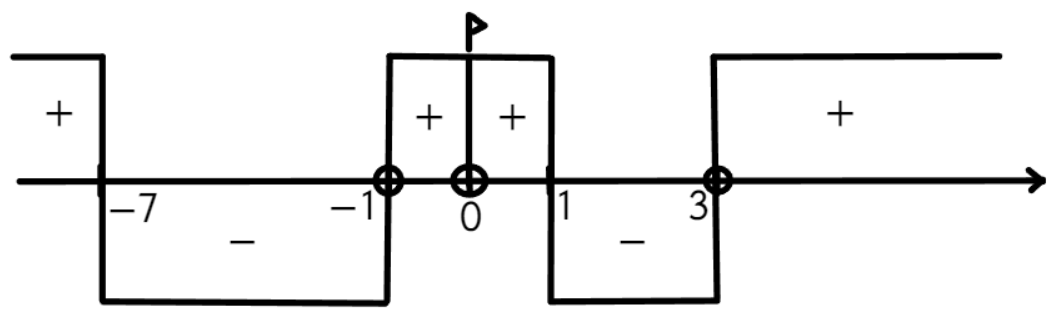
\includegraphics[scale=0.35]{ner9-63.png}}
\end{figure}\newpage\noindent
64. $|3x^2+12x-15|\leqslant15-12x-3x^2\Leftrightarrow\begin{cases}3x^2+12x-15\leqslant15-12x-3x^2,\\3x^2+12x-15\geqslant3x^2+12x-15.\end{cases}
\Leftrightarrow$\\$\begin{cases}6x^2+24x-30\leqslant0,\\0\geqslant0.\end{cases}\Leftrightarrow 6(x+5)(x-1)\leqslant0\Leftrightarrow x\in[-5;1].$\\
65. $|2x^2+15x-17|\leqslant17-15x-2x^2\Leftrightarrow\begin{cases}2x^2+15x-17\leqslant17-15x-2x^2,\\2x^2+15x-17\geqslant2x^2+15x-17.\end{cases}
\Leftrightarrow$\\$\begin{cases}4x^2+30x-34\leqslant0,\\0\geqslant0.\end{cases}\Leftrightarrow 2(x-1)(2x+17)\leqslant0\Leftrightarrow x\in\left[-\cfrac{17}{2};1\right].$\\
66. $\cfrac{(x^2-4x-1)(x^2-8x+16)}{(x^2+x)(x^2-16x+64)}\geqslant0\Leftrightarrow
\cfrac{(x-(2-\sqrt{5}))(x-(2+\sqrt{5}))(x-4)^2}{x(x+1)(x-8)^2}\geqslant0.$ Применив метод интервалов, найдём ответ: $x\in
(-\infty;-1)\cup[2-\sqrt{5};0)\cup\{4\}\cup[2+\sqrt{5};8)\cup(8;+\infty).$
\begin{figure}[ht!]
\center{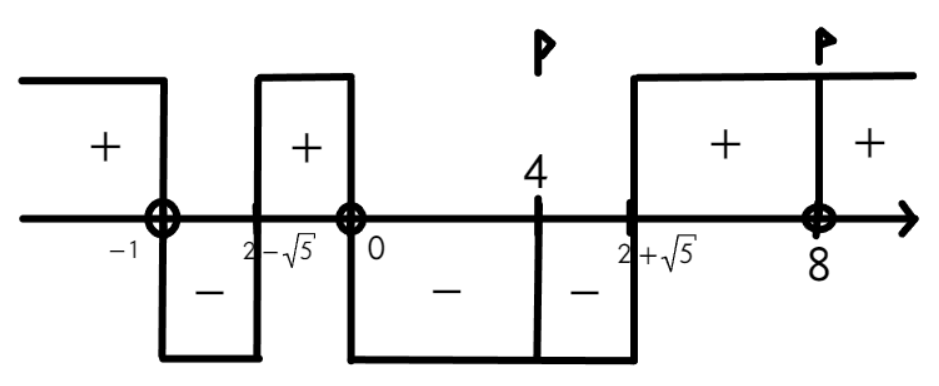
\includegraphics[scale=0.35]{ner9-66.png}}
\end{figure}\\
67. $\cfrac{(x^2+4x-1)(x^2+8x+16)}{(x^2-x)(x^2+16x+64)}\geqslant0\Leftrightarrow
\cfrac{(x-(-2-\sqrt{5}))(x-(\sqrt{5}-2))(x+4)^2}{x(x-1)(x+8)^2}\geqslant0.$ Применив метод интервалов, найдём ответ: $x\in
(-\infty;-8)\cup(-8;-2-\sqrt{5}]\cup\{-4\}\cup(0;\sqrt{5}-2]\cup(1;+\infty).$
\begin{figure}[ht!]
\center{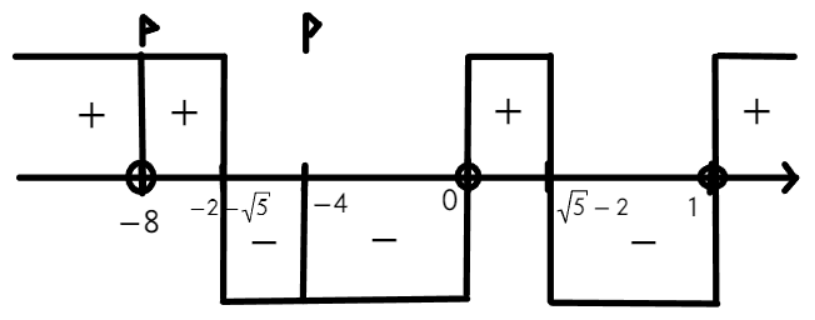
\includegraphics[scale=0.35]{ner9-67.png}}
\end{figure}\\
68. $\cfrac{(1-x^2)(x-1)^2(x+1)^3}{x^6-x^4+x^2}\leqslant0\Leftrightarrow\cfrac{-(x-1)^3(x+1)^4}{x^2(x^4-x^2+1)}\leqslant0.$ Применив метод интервалов, найдём ответ: $x\in\{-1\}\cup[1;+\infty).$
\begin{figure}[ht!]
\center{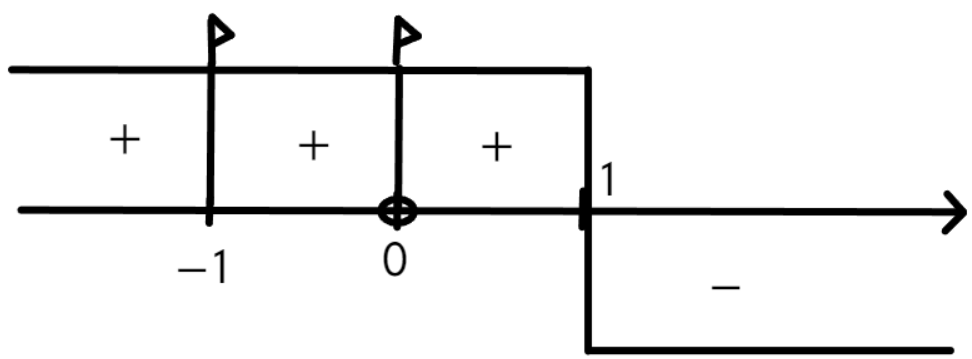
\includegraphics[scale=0.35]{ner9-32.png}}
\end{figure}\\
69. $|x-1|>3+x-|2-x|\Leftrightarrow |x-1|+|x-2|>x+3\Leftrightarrow\left[\begin{array}{l} \begin{cases} 1-x-x+2>x+3,\\
x\leqslant1.\end{cases}\\ \begin{cases} x-1-x+2>x+3,\\ 1<x<2.\end{cases} \\ \begin{cases} x-1+x-2>x+3,\\ 2\leqslant x.\end{cases}\end{array}\right.\Leftrightarrow
\left[\begin{array}{l} \begin{cases} x<0,\\
x\leqslant1.\end{cases}\\ \begin{cases} x<-2,\\ 1<x<2.\end{cases} \\ \begin{cases} x>6,\\ 2\leqslant x.\end{cases}\end{array}\right.\Leftrightarrow
x\in(-\infty;0)\cup(6;+\infty).$\\
70. $\cfrac{(x^2+3x-10)(x^2+3x+5)}{3x^2-7x+2}\geqslant0\Leftrightarrow\cfrac{(x+5)(x-2)((x+1,5)^2+2,75)}{(x-2)(3x-1)}\geqslant0.$ Применив метод интервалов, найдём ответ: $x\in(-\infty;-5]\cup\left(\cfrac{1}{3};2\right)\cup(2;+\infty).$
\begin{figure}[ht!]
\center{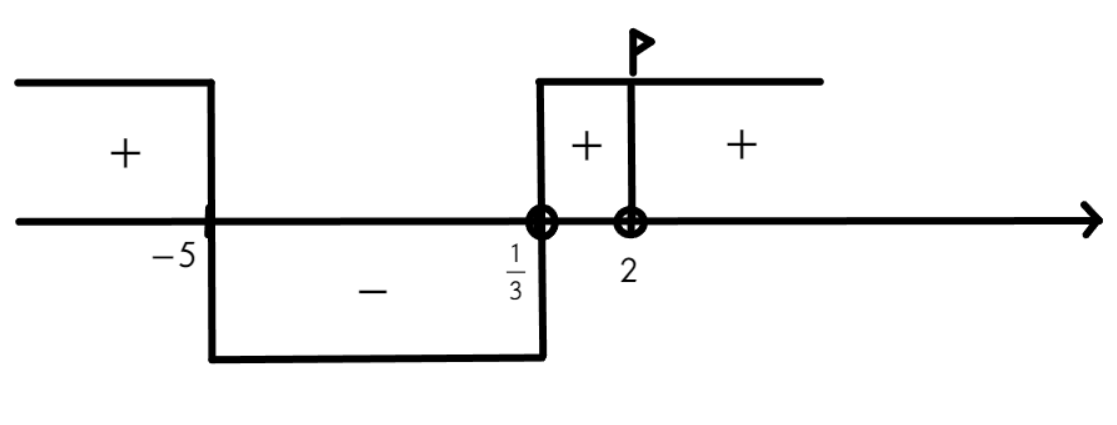
\includegraphics[scale=0.35]{ner9-70.png}}
\end{figure}\\
71. $3x+y>0$ и $x-3y>0,$ значит $y>-3x$ и $y<\cfrac{x}{3}.$\\
а) Если $x\leqslant0,$ то  из первого неравенства следует соотношение $y>0,$ а из второго --- $y<0,$ что невозможно. Значит, утверждение $x>0$ верно.\\
б) Утверждение неверно, например, при $x=1,\ y=-1.$\\
в) $3x+y>0$ и $x-3y>0,$ значит $x>-\cfrac{y}{3},\ x>3y.$ Если $y\geqslant0,$ то $x>3y>y.$ Если $y<0,$ то $x>-\cfrac{y}{3}>y.$ Значит, утверждение $x>y$ верно.\\
72. $$\begin{tikzpicture}[scale=0.5]
\begin{axis}[
    axis lines = middle,
    grid=major,
    legend pos={south west},
    xlabel = {$x$},
    %xlabel style={below right},
    ylabel = {$y$},
    ymin=-1,
    ymax=10,
    xtick={-2,-1,1,2, 3, 4},
    xticklabels={-2,-1,1,2, 3, 4},
    ytick={-2,-1,1, 3, 4},
    yticklabels={-2,-1,1, 3, 4},
                  ]
	\addplot[domain=-5:5, samples=100, color=black] {abs(x*x-2*x)};
    %\addplot[domain=-0.99:0.5, samples=100, color=black] {1/(1-x)};
    \addplot[domain=-5:5, samples=100, color=black] {x};
   % \addplot[domain=1.01:5, samples=100, color=black] {3/(x+1)};
    %\addlegendentry{$\text{Рис. 1}$};
\end{axis}
%\draw (2.75,2.82) circle (2pt);
%\draw (4.11,3.98) circle (2pt);
\end{tikzpicture}$$
 По графику найдём ответ $x \in [1;3]\cup\{0\}.$\\
73. $\cfrac{(x^2-3x+8)(x^2-3x+1)}{x^2-3x}\geqslant3.$ Сделаем замену $t=x^2-3x,$ тогда $\cfrac{(t+8)(t+1)}{t}\geqslant3\Leftrightarrow$\\$
\cfrac{t^2+t+8t+8-3t}{t}\geqslant0\Leftrightarrow \cfrac{t^2+6t+8}{t}\geqslant0\Leftrightarrow \cfrac{(t+2)(t+4)}{t}\geqslant0.$ Применив метод интервалов, найдём ответ: $t\in[-4;-2]\cup(0;+\infty).$
\begin{figure}[ht!]
\center{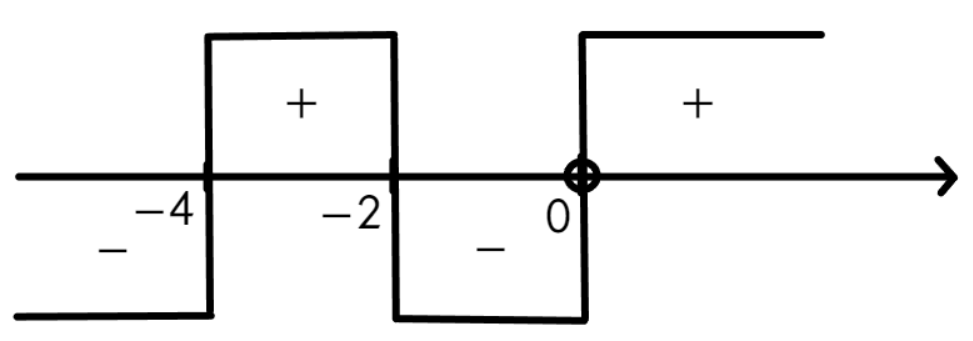
\includegraphics[scale=0.35]{ner9-73.png}}
\end{figure}\\
Теперь необходимо решить неравенства относительно $x:\ t\in[-4;-2]\Leftrightarrow\begin{cases} x^2-3x\geqslant-4,\\ x^2-3x\leqslant-2.\end{cases}
\Leftrightarrow\begin{cases} x^2-3x+4\geqslant0,\\ x^2-3x+2\leqslant0.\end{cases}\Leftrightarrow
\begin{cases} (x-1,5)^2+1,75\geqslant0,\\ (x-2)(x-1)\leqslant0.\end{cases}\Rightarrow x\in[1;2].$ Для второго интервала получим $t>0,\ x^2-3x>0,\ x(x-3)>0,\
x\in(-\infty;0)\cup(3;+\infty).$ Таким образом,  $x\in(-\infty;0)\cup[1;2]\cup(3;+\infty).$\\
74. $\cfrac{x\sqrt{x}+x-5\sqrt{x}+2}{\sqrt{x}-2}\geqslant x \Leftrightarrow \begin{cases} t=\sqrt{x}\geqslant0,\\ \cfrac{t^3+t^2-5t+2}{t-2}\geqslant t^2.\end{cases}
\Leftrightarrow \begin{cases} t=\sqrt{x}\geqslant0,\\ \cfrac{t^3+t^2-5t+2}{t-2}\geqslant t^2.\end{cases}
\Leftrightarrow$\\$ \begin{cases} t=\sqrt{x}\geqslant0,\\ \cfrac{t^3+t^2-5t+2-t^3+2t^2}{t-2}\geqslant 0.\end{cases}
\Leftrightarrow \begin{cases} t=\sqrt{x}\geqslant0,\\ \cfrac{3t^2-5t+2}{t-2}\geqslant 0.\end{cases}
\Leftrightarrow \begin{cases} t=\sqrt{x}\geqslant0,\\ \cfrac{(t-1)(3t-2)}{t-2}\geqslant 0.\end{cases}$ Применив метод интервалов, найдём ответ: $t\in\left[\cfrac{2}{3};1\right]\cup(2;+\infty)\Leftrightarrow x \in\left[\cfrac{4}{9};1\right]\cup(4;+\infty).$
\begin{figure}[ht!]
\center{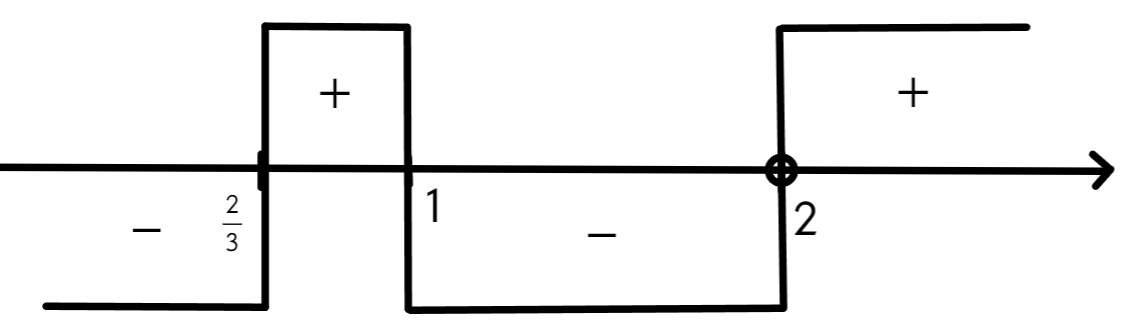
\includegraphics[scale=0.35]{int9-74.png}}
\end{figure}\\
75. $\cfrac{x\sqrt{x}-x-5\sqrt{x}+3}{\sqrt{x}-3}\geqslant x \Leftrightarrow \begin{cases} t=\sqrt{x}\geqslant0,\\ \cfrac{t^3-t^2-5t+3}{t-3}\geqslant t^2.\end{cases}
\Leftrightarrow \begin{cases} t=\sqrt{x}\geqslant0,\\ \cfrac{t^3+t^2-5t+2}{t-3}\geqslant t^2.\end{cases}
\Leftrightarrow$\\$ \begin{cases} t=\sqrt{x}\geqslant0,\\ \cfrac{t^3-t^2-5t+3-t^3+3t^2}{t-3}\geqslant 0.\end{cases}
\Leftrightarrow \begin{cases} t=\sqrt{x}\geqslant0,\\ \cfrac{2t^2-5t+3}{t-3}\geqslant 0.\end{cases}
\Leftrightarrow \begin{cases} t=\sqrt{x}\geqslant0,\\ \cfrac{(t-1)(2t-3)}{t-3}\geqslant 0.\end{cases}$ Применив метод интервалов, найдём ответ: $t\in\left[1;\cfrac{3}{2}\right]\cup(3;+\infty)\Leftrightarrow x \in\left[1;\cfrac{9}{4}\right]\cup(9;+\infty).$
\begin{figure}[ht!]
\center{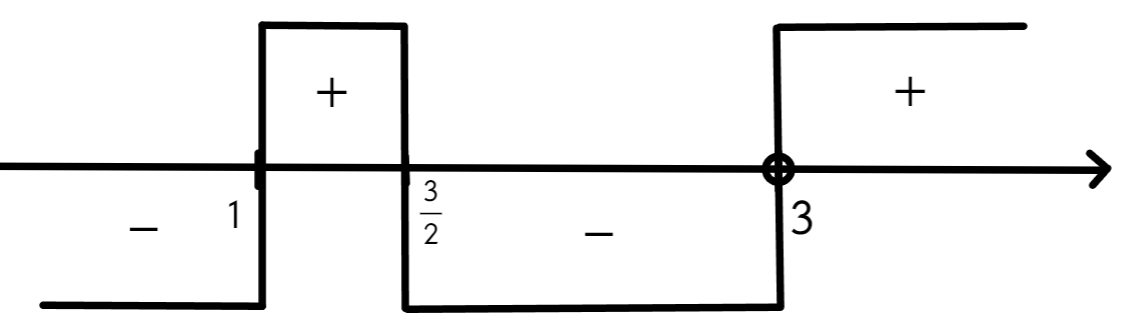
\includegraphics[scale=0.35]{ner9-75.png}}
\end{figure}\\
76. Если знаменатель правой части отрицателен $(x<2),$ то левая часть больше при любом $x$ из области определения: $x^2-5x+6=(x-2)(x-3)\neq0,\ x\neq2$ и $x\neq3.$ Значит, подходит интервал $(-\infty;2).$ Если знаменатель правой дроби положителен $(x>2),$ то необходимо выполнение неравенства $|x^2-5x+6|\leqslant x-2\Leftrightarrow \begin{cases} x^2-5x+6\leqslant x-2,\\ x^2-5x+6\geqslant 2-x.\end{cases}\Leftrightarrow \begin{cases} x^2-6x+8\leqslant0,\\ x^2-4x+4\geqslant0.\end{cases}
\Leftrightarrow \begin{cases} (x-2)(x-4)\leqslant0,\\ (x-2)^2\geqslant0.\end{cases}\Rightarrow x\in(2;3)\cup(3;4].$ Таким образом, итоговый ответ $x\in(-\infty;2)\cup (2;3)\cup(3;4].$\newpage\noindent
77. $\cfrac{(x^2-7x+10)(x^2-8x+16)}{\sqrt{x+10}(-2x^2+3x-10)}\leqslant 0\Leftrightarrow \cfrac{(x-5)(x-2)(x-4)^2}{\sqrt{x+10}(x^2+(x-1,5)^2+7,75)}\geqslant 0.$
Применив метод интервалов, найдём ответ: $x\in(-10;2]\cup\{4\}\cup[5;+\infty).$
\begin{figure}[ht!]
\center{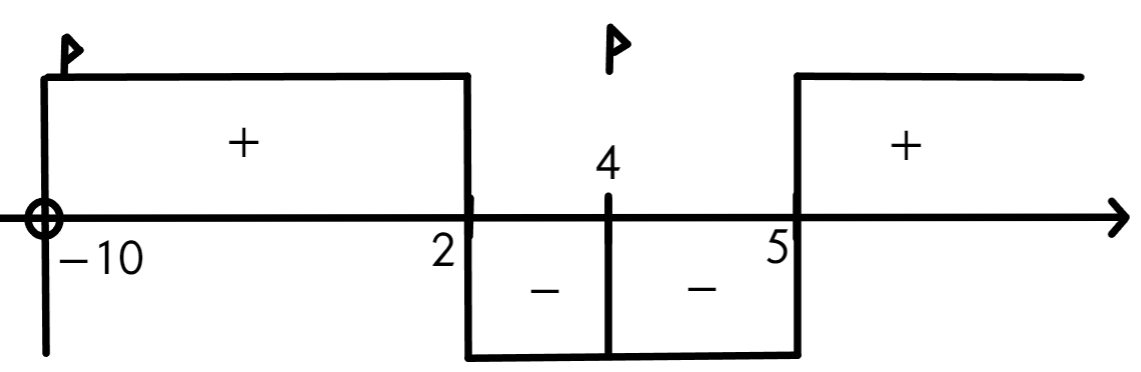
\includegraphics[scale=0.35]{ner9-77.png}}
\end{figure}\\
78. $(x-1)x(x+1)(x+2)\leqslant8\Leftrightarrow (x^2+x-2)(x^2+x)\leqslant8.$ Сделаем замену $t=x^2+x,$ тогда $(t-2)t\leqslant8\Leftrightarrow
t^2-2t-8\leqslant0\Leftrightarrow(t-4)(t+2)\leqslant0\Leftrightarrow t\in[-2;4]\Leftrightarrow \begin{cases} x^2+x\geqslant-2,\\ x^2+x\leqslant 4.\end{cases}
\Leftrightarrow \begin{cases} x^2+x+2\geqslant0,\\ x^2+x-4\leqslant 0.\end{cases}\Leftrightarrow \left(x-\cfrac{-1-\sqrt{17}}{2}\right)\left(x-\cfrac{-1+\sqrt{17}}{2}\right)\leqslant0\Leftrightarrow x\in \left[\cfrac{-1-\sqrt{17}}{2};\cfrac{-1+\sqrt{17}}{2}\right].$ Целыми решениями этого неравенства являются числа от $-2$ до 1, их сумма равна $-2.$\\
79. Пусть $t=\left|\cfrac{2x-1}{x+2}\right|\geqslant0.$ Тогда $t^2+t\geqslant12,\ (t-3)(t+4)\geqslant0,\ t\geqslant3.$ Значит, $\left|\cfrac{2x-1}{x+2}\right|\geqslant3\Leftrightarrow\left[\begin{array}{l}\cfrac{2x-1}{x+2}\geqslant3,\\ \cfrac{2x-1}{x+2}\leqslant-3.\end{array}\right.
\Leftrightarrow\left[\begin{array}{l}\cfrac{-x-7}{x+2}\geqslant0,\\ \cfrac{5x+5}{x+2}\leqslant0.\end{array}\right.
\Leftrightarrow\left[\begin{array}{l}\cfrac{x+7}{x+2}\leqslant0,\\ \cfrac{x+1}{x+2}\leqslant0.\end{array}\right.
\Leftrightarrow\left[\begin{array}{l}x\in[-7;-2),\\ x\in(-2;-1].\end{array}\right.\Leftrightarrow
x\in[-7;-2)\cup(-2;-1].$\\
80. Пусть $t=\left|\cfrac{2x+3}{x-2}\right|\geqslant0.$ Тогда $t^2\leqslant20+t,\ (t-5)(t+4)\leqslant0,\ t\leqslant5.$ Значит, $\left|\cfrac{2x+3}{x-2}\right|\leqslant5\Leftrightarrow\begin{cases}\cfrac{2x+3}{x-2}\leqslant5,\\ \cfrac{2x+3}{x-2}\geqslant-5.\end{cases}
\Leftrightarrow\begin{cases}\cfrac{-3x+13}{x-2}\leqslant0,\\ \cfrac{7x-7}{x-2}\geqslant0.\end{cases}
\Leftrightarrow\begin{cases}\cfrac{3x-13}{x-2}\geqslant0,\\ \cfrac{x-1}{x-2}\geqslant0.\end{cases}
\Leftrightarrow\begin{cases}x\in[-\infty;2)\cup\left[\cfrac{13}{3};+\infty\right),\\ x\in(-\infty;1]\cup(2;+\infty).\end{cases}\Leftrightarrow
x\in(-\infty;1]\cup\left[\cfrac{13}{3};+\infty\right).$\\
81. $\cfrac{(6-x-x^2)\sqrt{x-1}}{x-3}\geqslant0\Leftrightarrow\cfrac{(2-x)(x+3)\sqrt{x-1}}{x-3}\geqslant0.$ Применив метод интервалов, найдём ответ: $x\in\{1\}\cup[2;3).$
\begin{figure}[ht!]
\center{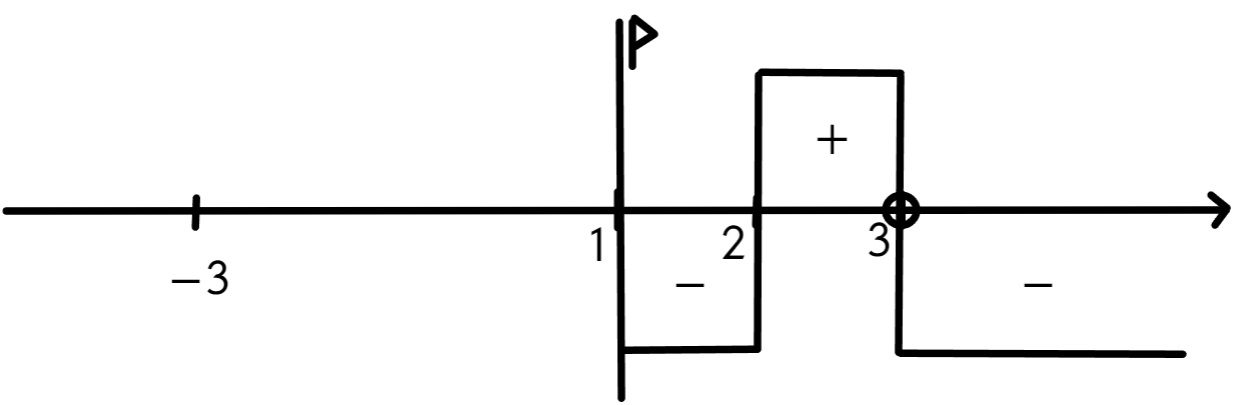
\includegraphics[scale=0.35]{ner9-82.png}}
\end{figure}\newpage\noindent
82. $\cfrac{(x^2+3x-18)\sqrt{5-x}}{1-x}\geqslant0\Leftrightarrow\cfrac{(x+6)(x-3)\sqrt{5-x}}{1-x}\geqslant0.$ Применив метод интервалов, найдём ответ: $x\in(-\infty;-6]\cup(1;3)\cup\{5\}.$
\begin{figure}[ht!]
\center{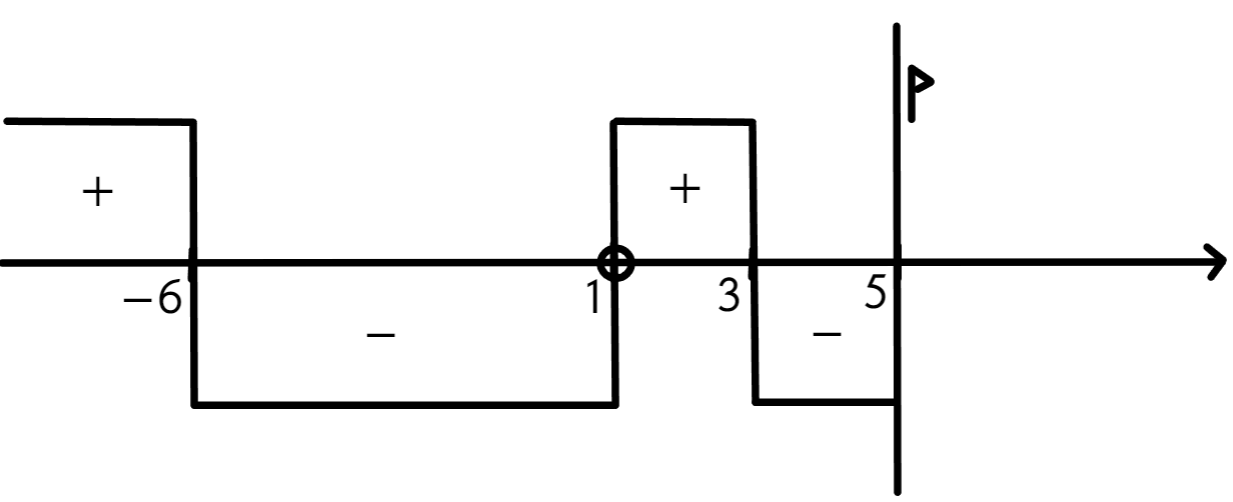
\includegraphics[scale=0.35]{ner9-83.png}}
\end{figure}\\
83. $(x^2-4x-5)\left(\cfrac{x}{x^2-5x+6}+\cfrac{5}{x^2-10x+21}+\cfrac{7}{(x-2)(x-3)(x-7)}\right)\geqslant0\Leftrightarrow$\\$
(x-5)(x+1)\left(\cfrac{x}{(x-2)(x-3)}+\cfrac{5}{(x-3)(x-7)}+\cfrac{7}{(x-2)(x-3)(x-7)}\right)\geqslant0\Leftrightarrow$\\$
(x-5)(x+1)\cdot\cfrac{x^2-7x+5x-10+7}{(x-2)(x-3)(x-7)}\geqslant0\Leftrightarrow
\cfrac{(x-5)(x+1)(x^2-2x-3)}{(x-2)(x-3)(x-7)}\geqslant0\Leftrightarrow
\cfrac{(x-5)(x+1)^2(x-3)}{(x-2)(x-3)(x-7)}\geqslant0.$ Применив метод интервалов, найдём ответ: $x\in\{-1\}\cup(2;3)\cup(3;5]\cup(7;+\infty).$
\begin{figure}[ht!]
\center{\includegraphics[scale=0.35]{ner9-833.png}}
\end{figure}\\
84. $\cfrac{|x+2|}{x^2-1}\leqslant-2\Rightarrow x^2-1<0\Rightarrow \begin{cases}x+2>0,\\ (x+1)(x-1)<0.\end{cases} \Rightarrow\begin{cases}|x+2|=x+2,\\ x\in (-1;1).\end{cases}.$ Тогда должно выполняться неравенство $x+2\geqslant 2-2x^2 \Leftrightarrow 2x^2+x \geqslant 0 \Leftrightarrow
x(2x+1)\geqslant 0 \Leftrightarrow x\in\left(\-\infty;-\cfrac{1}{2}\right]\cup[0;+\infty).$ С учётом ранее полученного ограничения имеем ответ $x\in \left(-1;-\cfrac{1}{2}\right]\cup[0;1).$\\
85. $\cfrac{|x+8|}{x^2-4}\leqslant-2\Rightarrow x^2-4<0\Rightarrow \begin{cases}x+8>0,\\ (x+2)(x-2)<0.\end{cases} \Rightarrow\begin{cases}|x+8|=x+8,\\ x\in (-2;2).\end{cases}.$ Тогда должно выполняться неравенство $x+8\geqslant 8-2x^2 \Leftrightarrow 2x^2+x \geqslant 0 \Leftrightarrow
x(2x+1)\geqslant 0 \Leftrightarrow x\in\left(\-\infty;-\cfrac{1}{2}\right]\cup[0;+\infty).$ С учётом ранее полученного ограничения имеем ответ $x\in \left(-2;-\cfrac{1}{2}\right]\cup[0;2).$\newpage\noindent
86. $\cfrac{(x-2)(x-3)^2}{x-1}\geqslant x^2-3x\Leftrightarrow \cfrac{(x-2)(x-3)^2-(x-3)x(x-1)}{x-1}\geqslant0\Leftrightarrow$\\
$\cfrac{(x-3)((x-2)(x-3)-x(x-1))}{x-1}\geqslant0\Leftrightarrow\cfrac{(x-3)(x^2-5x+6-x^2+x)}{x-1}\geqslant0
\Leftrightarrow \cfrac{2(x-3)(3-2x)}{x-1}\geqslant0.$ Применив метод интервалов, найдём ответ: $x\in(-\infty;1)\cup\left[\cfrac{3}{2};3\right].$
\begin{figure}[ht!]
\center{\includegraphics[scale=0.35]{ner9-84.png}}
\end{figure}\\
87. $\cfrac{(x+1)(x-2)^2}{x+2}\leqslant x^2-2x\Leftrightarrow \cfrac{(x+1)(x-2)^2-(x-2)x(x+2)}{x+2}\leqslant0\Leftrightarrow$\\
$\cfrac{(x-2)((x+1)(x-2)-x(x+2))}{x+2}\leqslant0\Leftrightarrow\cfrac{(x-2)(x^2-x-2-x^2-2x)}{x+2}\leqslant0
\Leftrightarrow \cfrac{(x-2)(3x+2)}{x+2}\geqslant0.$ Применив метод интервалов, найдём ответ: $x\in\left(-2;-\cfrac{2}{3}\right]\cup[2;+\infty).$
\begin{figure}[ht!]
\center{\includegraphics[scale=0.35]{ner9-85.png}}
\end{figure}\\
88. $2x^2+4xy+4y^2+1\leqslant 2x\Leftrightarrow x^2-2x+1+x^2+4xy+4y^2\leqslant0
\Leftrightarrow (x-1)^2+(x+2y)^2\leqslant0 \Leftrightarrow \begin{cases} x=1,\\ x+2y=0.\end{cases} \Leftrightarrow \begin{cases} x=1,\\ y=-\cfrac{1}{2}.\end{cases}$\\
89.  $\cfrac{2|x|}{x+1}>-x.$ Если $x>0,$ то левая часть неравенства положительна, а правая отрицательна, поэтому все $x>0$ подходят и надо разобрать только случай $x<0$ (тогда $|x|=-x$). Значение $x=0$ не подходит, так как в этом случае левая часть равна правой.

$\cfrac{-2x}{x+1}>-x\Leftrightarrow \cfrac{-2x+x^2+x}{x+1}>0\Leftrightarrow \cfrac{x(x-1)}{x+1}>0.$ Так как $x<0,$ то и $x-1<0,$ а значит необходимо, чтобы выполнялось неравенство $x+1>0,$ то есть $x>-1.$ Таким образом, окончательным ответом является $x\in(-1;0)\cup (0;+\infty).$\\
90. $\cfrac{(2x^2+4x)(3x-x^2)}{(2x+5)^3}\leqslant 0\Leftrightarrow
\cfrac{2x(x+2)x(3-x)}{(2x+5)^3}\leqslant0\Leftrightarrow
\cfrac{x^2(x+2)(x-3)}{(2x+5)^3}\geqslant0.$ Применив метод интервалов, найдём ответ: $x\in\left(-\cfrac{5}{2};-2\right]\cup\{0\}\cup[3;+\infty).$
\begin{figure}[ht!]
\center{\includegraphics[scale=0.35]{ner9-86.png}}
\end{figure}\\
91. $\cfrac{(x-x^2)(3x^2+15x)}{(2x-7)^3}\geqslant 0\Leftrightarrow
\cfrac{x(1-x)3x(x+5)}{(2x-7)^3}\geqslant0\Leftrightarrow
\cfrac{x^2(x+5)(x-1)}{(2x-7)^3}\leqslant0.$ Применив метод интервалов, найдём ответ: $x\in\left(-\infty;-5\right]\cup\{0\}\cup\left[1;\cfrac{7}{2}\right).$
\begin{figure}[ht!]
\center{\includegraphics[scale=0.35]{ner9-87.png}}
\end{figure}\\
92. $\left|\cfrac{x-3}{x+4}\right|<1\Leftrightarrow
\begin{cases} \cfrac{x-3}{x+4}<1,\\
\cfrac{x-3}{x+4}>-1.\end{cases}\Leftrightarrow
\begin{cases} \cfrac{x-3-x-4}{x+4}<0,\\
\cfrac{x-3+x+4}{x+4}>0.\end{cases}\Leftrightarrow
\begin{cases} \cfrac{-7}{x+4}<0,\\
\cfrac{2x+1}{x+4}>0.\end{cases}\Leftrightarrow$\\$
\begin{cases} x>-4,\\
x\in(-\infty;-4)\cup\left(-\cfrac{1}{2};+\infty\right).\end{cases}\Leftrightarrow
x\in\left(-\cfrac{1}{2};+\infty\right).$\\
93. $\left|\cfrac{2x+1}{x-1}\right|>2\Leftrightarrow
\left[\begin{array}{l} \cfrac{2x+1}{x-1}>2,\\ \cfrac{2x+1}{x-1}<-2.\end{array}\right.\Leftrightarrow
\left[\begin{array}{l} \cfrac{2x+1-2x+2}{x-1}>0,\\ \cfrac{2x+1+2x-2}{x-1}<0.\end{array}\right.\Leftrightarrow
\left[\begin{array}{l} \cfrac{3}{x-1}>0,\\ \cfrac{4x-1}{x-1}<0.\end{array}\right.\Leftrightarrow$\\$
\left[\begin{array}{l} x>1,\\ x\in\left(\cfrac{1}{4}; 1\right).\end{array}\right.\Leftrightarrow x\in\left(\cfrac{1}{4}; 1\right)\cup(1;+\infty).$\\
94. $\cfrac{3x^2+6x+2}{x^2+2x}+\cfrac{2x+2}{x-1}\geqslant\cfrac{5x+1}{x}
\Leftrightarrow 3+\cfrac{2}{x^2+2x}+2+\cfrac{4}{x-1}\geqslant 5+\cfrac{1}{x}
\Leftrightarrow \cfrac{2}{x(x+2)}+\cfrac{4}{x-1}-\cfrac{1}{x}\geqslant0
\Leftrightarrow \cfrac{2(x-1)+4x(x+2)-(x-1)(x+2)}{x(x+2)(x-1)}\geqslant0
\Leftrightarrow \cfrac{2x-2+4x^2+8x-x^2-2x+x+2}{x(x+2)(x-1)}\geqslant0
\Leftrightarrow \cfrac{3x^2+9x}{x(x+2)(x-1)}\geqslant0
\Leftrightarrow \cfrac{3x(x+3)}{x(x+2)(x-1)}\geqslant0.$ Применив метод интервалов, найдём ответ: $x\in[-3;-2)\cup(1;+\infty).$
\begin{figure}[ht!]
\center{\includegraphics[scale=0.35]{ner9-38.png}}
\end{figure}\\
95. $\cfrac{(-1+x^2)(x+1)^2(x-1)^3}{x^8-x^6+x^4}\leqslant0\Leftrightarrow\cfrac{(x-1)^4(x+1)^3}{x^4(x^4-x^2+1)}\leqslant0.$ Применив метод интервалов, найдём ответ: $x\in(-\infty;-1]\cup\{1\}.$
\begin{figure}[ht!]
\center{\includegraphics[scale=0.35]{ner99-33.png}}
\end{figure}
\newpage
\section{Исследование функций и уравнений решения}
1. По теореме Виета $x_1+x_2=10,\ x_1x_2=q.$ Тогда $x_1^2+x_2^2=(x_1+x_2)^2-2x_1x_2=100-2q=2\Rightarrow q=49.$ Дискриминант уравнения в этом случае равен -171, а значит корней нет и таких $q$ не существует.\\
2. По теореме Виета $x_1+x_2=6,\ x_1x_2=q.$ Тогда $x_1^2+x_2^2=(x_1+x_2)^2-2x_1x_2=36-2q=4\Rightarrow q=16.$ Дискриминант уравнения в этом случае равен -28, а значит корней нет и таких $q$ не существует.\\
3. Первое уравнение задаёт на плоскости прямую, а второе --- окружность. Они могут иметь 0, 1 или 2 точки пересечения.\\
4. Первое уравнение задаёт на плоскости прямую, а второе --- окружность. Они могут иметь 0, 1 или 2 точки пересечения.\\
5. Для нахождения области определения $f(x)$ необходимо решить неравенство\\ $\cfrac{x(x^2+x-12)(x^2-3x+2)}{(x^2-x-6)(-x+5)}\geqslant0
\Leftrightarrow \cfrac{x(x+4)(x-3)(x-2)(x-1)}{(x-3)(x+2)(-x+5)}\geqslant0.$ Решим его, применив метод интервалов:
$x\in[-4;-2)\cup[0;1]\cup[2;3)\cup(3;5).$
\begin{figure}[ht!]
\center{\includegraphics[scale=0.35]{isl9-5.png}}
\end{figure}\\
6. Для нахождения области определения $f(x)$ необходимо решить неравенство\\ $\cfrac{-x(x^2-2x-15)(x^2-6x+8)}{(x^2-11x+30)(x+1)}\geqslant0
\Leftrightarrow \cfrac{-x(x-5)(x+3)(x-2)(x-4)}{(x-5)(x+6)(x+1)}\geqslant0.$ Решим его, применив метод интервалов:
$x\in[-3;-1)\cup[0;2]\cup[4;5)\cup(5;6).$
\begin{figure}[ht!]
\center{\includegraphics[scale=0.35]{isl9-6.png}}
\end{figure}\\
7. Если корнями уравнения являются числа $x_1$ и $x_2=x_1^2,$ то по теореме Виета имеем равенство $x_1\cdot x_1^2=x_1^3=a^3,$ откуда $x_1=a,\ x_2=a^2.$ По теореме Виета эти числа будут являться корнями уравнения тогда и только тогда, когда $a+a^2=\cfrac{15}{4},\ 4a^2+4a-15=0,\ a=\cfrac{3}{2}$ или $a=-\cfrac{5}{2}.$\\
8. Если корнями уравнения являются числа $x_1$ и $x_2=x_1^2,$ то по теореме Виета имеем равенство $x_1\cdot x_1^2=x_1^3=a^3,$ откуда $x_1=a,\ x_2=a^2.$ По теореме Виета эти числа будут являться корнями уравнения тогда и только тогда, когда $a+a^2=\cfrac{63}{4},\ 4a^2+4a-63=0,\ a=\cfrac{7}{2}$ или $a=-\cfrac{9}{2}.$\\
9. Для нахождения области определения $f(x)$ необходимо решить систему $\begin{cases} 4+3x-x^2>0,\\ x-2\neq0.\end{cases}\Leftrightarrow
\begin{cases} (x-4)(x+1)<0,\\ x\neq2.\end{cases}\Leftrightarrow x\in(-1;2)\cup(2;4).$\\
10. Для нахождения области определения $f(x)$ необходимо решить систему $\begin{cases} 3+2x-x^2>0,\\ x-1\neq0.\end{cases}\Leftrightarrow
\begin{cases} (x-3)(x+1)<0,\\ x\neq1.\end{cases}\Leftrightarrow x\in(-1;1)\cup(1;3).$\\
11. Пусть корни уравнения равны $a$ и $a+2,$ тогда по теореме Виета $a(a+2)=15,\ a^2+2a-15=0,\ a=3$ или $a=-5.$ То есть корнями могут быть числа 3 и 5 или $-5$ и $-3.$ По той же теореме Виета имеем равенство $3+5=k,$ то есть $k=8$ или $(-3)+(-5)=k,$ то есть $k=-8.$\\
12. Пусть корни уравнения равны $a$ и $a+2,$ тогда по теореме Виета $a(a+2)=3,\ a^2+2a-3=0,\ a=1$ или $a=-3.$ То есть корнями могут быть числа 1 и 3 или $-3$ и $-1.$ По той же теореме Виета имеем равенство $1+3=k,$ то есть $k=4$ или $(-1)+(-3)=k,$ то есть $k=-4.$\\
13. Уравнение имеет два различных корня, если $k\neq0$ и $D>0,$ то есть $(k+1)^2-4k(2k-1)=k^2+2k+1-8k^2+4k=-7k^2+6k+1>0,\ 7k^2-6k-1<0,\ (7k+1)(k-1)<0,\ k\in\left(-\cfrac{1}{7};1\right).$ Таким образом, $k\in\left(-\cfrac{1}{7};0\right)\cup(0;1).$\\
14. Уравнение имеет два различных корня, если $k\neq0$ и $D>0,$ то есть $(k-1)^2-4k(2k+1)=k^2-2k+1-8k^2-4k=-7k^2-6k+1>0,\ 7k^2+6k-1<0,\ (7k-1)(k+1)<0,\ k\in\left(-1;\cfrac{1}{7}\right).$ Таким образом, $k\in\left(-1;0\right)\cup\left(0;\cfrac{1}{7}\right).$\\
15. $y=-x+2\sqrt{x}-2=-((\sqrt{x})^2-2\sqrt{x}+1)-1=-(\sqrt{x}-1)^2-1\leqslant-1.$\\
16. $y=-x+4\sqrt{x}-5=-((\sqrt{x})^2-4\sqrt{x}+4)-1=-(\sqrt{x}-2)^2-1\leqslant-1.$\\
17. Пусть $t=2x-3,$ тогда $x=\cfrac{t+3}{2}$ и $f(t)=4\cdot\cfrac{t+3}{2}-5=2t+1$ Таким образом, $f(x)=2x+1.$\\
18. Пусть $t=2x+3,$ тогда $x=\cfrac{t-3}{2}$ и $f(t)=4\cdot\cfrac{t-3}{2}+5=2t-1$ Таким образом, $f(x)=2x-1.$\\
19. Уравнение имеет ровно один корень либо если $2a=0,\ a=0,$ либо если $D=(10-a)^2-8a(-a+5)=a^2-20a+100+8a^2-40a=9a^2-60a+100=(3a-10)^2=0,\ a=\cfrac{10}{3}.$\\
20. Уравнение имеет ровно один корень либо если $2a=0,\ a=0,$ либо если $D=(10+a)^2-8a(-a-5)=a^2+20a+100+8a^2+40a=9a^2+60a+100=(3a+10)^2=0,\ a=-\cfrac{10}{3}.$\\
21. По теореме Виета $x_1+x_2=\cfrac{3}{2},\ x_1x_2=-\cfrac{11}{2}.$ Тогда $\cfrac{x_2}{1+x_1}+\cfrac{x_1}{1+x_2}=\cfrac{x_2+x_2^2+x_1+x_1^2}{1+x_1+x_2+x_1x_2}=
\cfrac{(x_1+x_2)^2+x_1+x_2-2x_1x_2}{1+x_1+x_2+x_1x_2}=\cfrac{\cfrac{9}{4}+\cfrac{3}{2}+11}{1+\cfrac{3}{2}-\cfrac{11}{2}}=-\cfrac{59}{12}.$\\
22. По теореме Виета $x_1+x_2=-2,\ x_1x_2=-\cfrac{8}{9}.$ Тогда $x_1^3+x_2^3=(x_1+x_2)(x_1^2-x_1x_2+x_2^2)=(x_1+x_2)((x_1+x_2)^2-3x_1x_2)=(-2)\left(4+\cfrac{8}{3}\right)=-\cfrac{40}{3}.$\\
23. Корни уравнения лежат по разные стороны от 1 тогда и только тогда, когда выполняется неравенство $(x_1-1)(x_2-1)<0,\ x_1x_2-(x_1+x_2)+1<0.$ По теореме Виета имеем равенства $x_1+x_2=\cfrac{2a+1}{1-a^2},\ x_1x_2=\cfrac{3}{1-a^2}.$ Поэтому $\cfrac{3}{1-a^2}-\cfrac{2a+1}{1-a^2}+1<0,\
\cfrac{3-2a-a^2}{1-a^2}<0,\ \cfrac{(a+3)(a-1)}{(a-1)(a+1)}<0,\ a\in(-3;-1).$ Кроме того, необходимо проверить, что при этих значениях $a$ уравнение имеет два корня. Старший коэффициент обнуляется при $a=\pm1,$ которые в полученные интервал не входят. Остаётся проверить неравенство $D>0,$ то есть $(2a+1)^2+12(a^2-1)>0,$ что верно, так как квадрат всегда неотрицателен, а $a^2$ при полученных значениях $a$ больше 1.\\
24. Корни уравнения лежат по разные стороны от $(-1)$ тогда и только тогда, когда выполняется неравенство $(x_1+1)(x_2+1)<0,\ x_1x_2+(x_1+x_2)+1<0.$ По теореме Виета имеем равенства $x_1+x_2=\cfrac{3b-1}{4-b^2},\ x_1x_2=\cfrac{7}{4-b^2}.$ Поэтому $\cfrac{7}{4-b^2}+\cfrac{3b-1}{4-b^2}+1<0,\
\cfrac{10+3b-b^2}{4-b^2}<0,\ \cfrac{(b+2)(b-5)}{(b-2)(b+2)}<0,\ b\in(2;5).$ Кроме того, необходимо проверить, что при этих значениях $b$ уравнение имеет два корня. Старший коэффициент обнуляется при $b=\pm2,$ которые в полученные интервал не входят. Остаётся проверить неравенство $D>0,$ то есть $(3b-1)^2+28(b^2-4)>0,$ что верно, так как квадрат всегда неотрицателен, а $b^2$ при полученных значениях $b$ больше 4.\\
25. Наименьшее значение параболы достигается в вершине $x=-\cfrac{-6}{2}=3,$ значит $9-18+a=1,\ a=10.$\\
26. Наибольшее значение параболы достигается в вершине $x=-\cfrac{4}{-2}=2,$ значит $-4+8+a=2,\ a=-2.$\\
27. Парабола неотрицательна на отрезке, если её старший коэффициент отрицателен, и она имеет два корня. То есть необходимо решить систему неравенств $\begin{cases} a-3<0,\\ (a+1)^2-4(a-3)(a+1)>0.\end{cases}\Leftrightarrow\begin{cases} a<3,\\ a^2+2a+1-4a^2+8a+12>0.\end{cases}\Leftrightarrow
\begin{cases} a<3,\\ 3a^2-10a-13<0.\end{cases}\Leftrightarrow\begin{cases} a<3,\\ (a+1)(3a-13)<0.\end{cases}\Leftrightarrow$\\$
\begin{cases} a<3,\\ a\in\left(-1;\cfrac{13}{3}\right).\end{cases}\Leftrightarrow a\in(-1;3).$\\
28. Парабола неотрицательна на отрезке, если её старший коэффициент отрицателен, и она имеет два корня. То есть необходимо решить систему неравенств $\begin{cases} a+2<0,\\ (a-1)^2-4(a+2)(a-1)>0.\end{cases}\Leftrightarrow\begin{cases} a<-2,\\ a^2-2a+1-4a^2-4a+8>0.\end{cases}\Leftrightarrow
\begin{cases} a<-2,\\ 3a^2+6a-9<0.\end{cases}\Leftrightarrow\begin{cases} a<3,\\ 3(a-1)(a+3)<0.\end{cases}\Leftrightarrow$\\$
\begin{cases} a<-2,\\ a\in\left(-3;1\right).\end{cases}\Leftrightarrow a\in(-3;-2).$\\
29. Наибольшее значение достигается при $m=-3,\ n=2$ и равно $9-2=7.$ Наименьшее значение достигается при $m=-\cfrac{\sqrt{2}}{2},\ n=1,6$ и равно $\cfrac{1}{2}-\cfrac{5}{2}=-2.$\\
30. Наибольшее значение достигается при $a=-1,5,\ b=2,4$ и равно $2,4-0,9=1,5.$ Наименьшее значение достигается при $a=-5,\ b=-0,5$ и равно $-0,5-10=-10,5.$\\
31. Корни уравнения лежат по разные стороны от 2 тогда и только тогда, когда выполняется неравенство $(x_1-2)(x_2-2)<0,\ x_1x_2-2(x_1+x_2)+4<0.$ По теореме Виета имеем равенства $x_1+x_2=5-a,\ x_1x_2=a^2-a.$ Поэтому $a^2-a+2a-10+4<0,\
a^2+a-6<0,\ (a+3)(a-2)<0,\ a\in(-3;2).$ Кроме того, необходимо проверить, что при этих значениях $a$ уравнение имеет два корня. Для это рассмотрим неравенство $D>0,$ то есть $(a-5)^2-4(a^2-a)>0,\ a^2-10a+25-4a^2+4a>0,\ 3a^2+6a-25<0,\ 3(a+1)^2<28.$ При полученных ранее значениях $a$ это неравенство выполняется, так как максимальное значение левой части равно $3\cdot9=27<28.$\\
32. Корни уравнения лежат по разные стороны от $(-1)$ тогда и только тогда, когда выполняется неравенство $(x_1+1)(x_2+1)<0,\ x_1x_2+(x_1+x_2)+1<0.$ По теореме Виета имеем равенства $x_1+x_2=a-7,\ x_1x_2=a^2-6a.$ Поэтому $a^2-6a+a-7+1<0,\ a^2-5a-6<0,\ (a-6)(a+1)<0,\ a\in(-1;6).$ Кроме того, необходимо проверить, что при этих значениях $a$ уравнение имеет два корня. Для это рассмотрим неравенство $D>0,$ то есть $(a-7)^2-4(a^2-6a)>0,\ a^2-14a+49-4a^2+24a>0,\ 3a^2-10a-49<0,\ \left(a-\cfrac{5}{3}\right)^2<\cfrac{172}{9}.$ При полученных ранее значениях $a$ это неравенство выполняется, так как максимальное значение левой части равно $\left(6-\cfrac{5}{3}\right)^2=\cfrac{169}{9}<\cfrac{172}{9}.$\\
33. Решим неравенство: $1,6+13t-5t^2\geqslant4,\ 5t^2-12t+2,4\leqslant0,\ 5(t-2,4)(t-0,2)\leqslant0,\ t\in[0,2;2,4].$ Значит, мяч будет находиться на высоте не менее 4 метров в течение $2,4-0,2=2,2$с.\\
34. Решим неравенство: $1,4+9t-5t^2\geqslant3,\ 5t^2-9t+1,6\leqslant0,\ 5(t-1,6)(t-0,2)\leqslant0,\ t\in[0,2;1,6].$ Значит, мяч будет находиться на высоте не менее 3 метров в течение $1,6-0,2=1,4$с.\\
35. Корни квадратного уравнения расположены симметрично относительно вершины параболы, значит $-\cfrac{a^2+5a-2}{2a}=-2,\ a^2+5a-2=4a,\ a^2+a-2=0,\ a=-2$ или $a=1.$ Для найденных значений $a$ необходимо проверить количество корней. При $a=-2$ получаем уравнение $-2x^2+(4-10-2)x-2+4=0,\ 2x^2+8x-2=0,\ D>0.$ При $a=1$ получаем уравнение $x^2+(1+5-2)x+1+4=0,\ x^2+4x+5=0,\ D<0.$ Значит, подходит только $a=-2.$\\
36. Корни квадратного уравнения расположены симметрично относительно вершины параболы, значит $-\cfrac{a^2+a-2}{2a}=-1,\ a^2+a-2=2a,\ a^2-a-2=0,\ a=-1$ или $a=2.$ Для найденных значений $a$ необходимо проверить количество корней. При $a=-1$ получаем уравнение $-x^2+(1-1-2)x-1+4=0,\ x^2+2x-3=0,\ D>0.$ При $a=2$ получаем уравнение $2x^2+(4+2-2)x+2+4=0,\ 2x^2+4x+6=0,\ D<0.$ Значит, подходит только $a=-1.$\\
37. $y=7+\sqrt{x^2-2x+5}=7+\sqrt{(x-1)^2+4}\geqslant7+2=9.$\\
38. $y=6+\sqrt{3-x^2-2x}=6+\sqrt{4-(x+1)^2}\geqslant6+0=6.$\\
39. Уравнение $ax^2+(4a+2)x+3a+1,5=0$ имеет единственный корень либо если $a=0,$ либо если $\cfrac{D}{4}=0,\ (2a+1)^2-a(3a+1,5)=4a^2+4a+1-3a^2-1,5a=a^2+2,5a+1=0,\
a=-2$ или $a=-\cfrac{1}{2}.$\\
40. Уравнение $ax^2-(2a+6)x+3a+3=0$ имеет единственный корень либо если $a=0,$ либо если $\cfrac{D}{4}=0,\ (a+3)^2-a(3a+3)=a^2+6a+9-3a^2-3a=-2a^2+3a+9=0,\
a=3$ или $a=-\cfrac{3}{2}.$\\
41. $23-\cfrac{16}{x^2-2x+5}=23-\cfrac{16}{(x-1)^2+4}\geqslant23-\cfrac{16}{4}=19.$\\
42. $5+\cfrac{16}{x^2+2x+5}=5+\cfrac{16}{(x+1)^2+4}\geqslant5+\cfrac{16}{4}=9.$\\
43. Если $x-y=3,$ то $x=y+3.$ Тогда $x^2-4xy+y^2=(y+3)^2-4y(y+3)+y^2=y^2+6y+9-4y^2-12y+y^2=-2y^2-6y+9=-2(y^2+3y+2,25)+13,5=
-2(y+1,5)^2+13,5\leqslant13,5.$\\
44. Если $2x-y=1,$ то $y=2x-1.$ Тогда $5x^2+4xy-5y^2=5x^2+4x(2x-1)-5(2x-1)^2=5x^2+8x^2-4x-20x^2+20x-5=-7x^2+16x-5=-7\left(x^2-\cfrac{16}{7}x+\cfrac{64}{49}\right)+\cfrac{29}{7}=
-7\left(x-\cfrac{16}{7}\right)^2+\cfrac{29}{7}\leqslant\cfrac{29}{7}.$\\
45. $x^3+6x^2+ax=0,\ x(x^2+6x+a)=0.$ Это уравнение всегда имеет корень $x=0.$ Всего у уравнения два корня либо если один из корней уравнения $x^2+6x+a=0$ также равен нулю, либо если у него один (другой) корень. В первом случае $0+0+a=0,\ a=0,$ а во втором случае $\cfrac{D}{4}=9-a=0,\ a=9.$\\
46. $4x^3+4x^2+ax=0,\ x(4x^2+4x+a)=0.$ Это уравнение всегда имеет корень $x=0.$ Всего у уравнения два корня либо если один из корней уравнения $4x^2+4x+a=0$ также равен нулю, либо если у него один (другой) корень. В первом случае $0+0+a=0,\ a=0,$ а во втором случае $\cfrac{D}{4}=4-4a=0,\ a=1.$\\
47. $(\sqrt{19-a}+\sqrt{10-a})(\sqrt{19-a}-\sqrt{10-a})=19-a-(10-a)=9,$ значит $\sqrt{19-a}+\sqrt{10-a}=9:1=9.$\\
48. $(\sqrt{13-a}+\sqrt{6-a})(\sqrt{13-a}-\sqrt{6-a})=13-a-(6-a)=7,$ значит $\sqrt{13-a}+\sqrt{6-a}=7:1=7.$\\
49. Подставим $x=3$ и воспользуемся нечётностью функции, тогда $3f(2)+2f(-2)=2\cdot3+1,\ 3f(2)-2f(2)=7,\ f(2)=7.$\\
50. Подставим $x=5$ и воспользуемся нечётностью функции, тогда $2f(3)+5f(-3)=2\cdot5-1,\ 2f(3)-5f(3)=9,\ f(3)=-3.$\\
51. Пусть $f(x)=ax^2+bx+c,$ тогда получим систему уравнений $\begin{cases}a+b+c=1,\\ 9a+3b+c=27,\\ 16a+4b+c=64.\end{cases}$ Вычтем из второго уравнения первое, получим соотношение $8a+2b=26,\ b=13-4a.$ Вычтем из третьего уравнения первое и подставим вместо $b$ выражение $13-4a:\ 15a+3b=63,\ 5a+b=21,\ 5a+13-4a=21,\ a=8.$ Тогда $b=13-4\cdot8=-19,\ c=1-a-b=1-8+19=12.$ Таким образом, $f(x)=8x^2-19x+12.$\\
52. Пусть $f(x)=ax^2+bx+c,$ тогда получим систему уравнений $\begin{cases}a+b+c=1,\\ 4a+2b+c=8,\\ 16a+4b+c=64.\end{cases}$ Вычтем из второго уравнения первое, получим соотношение $3a+b=7,\ b=7-3a.$ Вычтем из третьего уравнения первое и подставим вместо $b$ выражение $7-3a:\ 15a+3b=63,\ 5a+b=21,\ 5a+7-3a=21,\ a=7.$ Тогда $b=7-3\cdot7=-14,\ c=1-a-b=1-7+14=8.$ Таким образом, $f(x)=7x^2-14x+8.$\\
53. Для нахождения области определения функции необходимо решить систему:\\ $\begin{cases} |x-1|(3x-6)\geqslant0,\\ x^2+4x-21\neq0.\end{cases}\Leftrightarrow
\begin{cases} \left[\begin{array}{l} x=1,\\ x\geqslant2.\end{array}\right.\\ x\neq-7,\ x\neq3.\end{cases}\Leftrightarrow x\in \{1\}\cup[2;3)\cup(3;+\infty).$\\
54. $y=\cfrac{(x+6)(x^3-27)}{x^2+3x-18}=\cfrac{(x+6)(x-3)(x^2+3x+9)}{(x+6)(x-3)}=x^2+3x+9,\ x\neq-6,\ x\neq3.$ Наименьшее значение парабола достигает в вершине $x_{\text{верш}}=-\cfrac{3}{2}$ и оно равно $\cfrac{9}{4}-\cfrac{9}{2}+9=\cfrac{27}{4}.$ При $x=-6$ и $x=3$ получим значения $36-18+9=27$ и $9+9+9=27.$ Значит, множество значений функции --- это $\left[\cfrac{27}{4};27\right)\cup(27;+\infty).$\\
55. Корни уравнения лежат по разные стороны от 1 тогда и только тогда, когда выполняется неравенство $(x_1-1)(x_2-1)<0,\ x_1x_2-(x_1+x_2)+1<0.$ По теореме Виета имеем равенства $x_1+x_2=2b+3,\ x_1x_2=-b-6.$ Поэтому $-b-6-2b-3+1<0,\
b>-\cfrac{8}{3}.$ Кроме того, необходимо проверить, что при этих значениях $b$ уравнение имеет два корня. Решим неравенство $D>0,$ то есть $(2b+3)^2+4(b+6)>0,\
4b^2+12b+9+4b+24>0,\ 4b^2+16b+33=(2b+4)^2+17>0.$ Оно выполняется при любых значениях $b,$ значит $b\in\left(-\cfrac{8}{3};+\infty\right).$\\
56. Решим данное уравнение графически. Правая часть представляет из себя гиперболу, а левая --- модуль, коэффициент при котором влияет на то, насколько большой угол при вершине $(5;0)$ будет образован.
$$\begin{tikzpicture}[scale=0.5]
\begin{axis}[
    axis lines = middle,
    grid=major,
    legend pos={south west},
    xlabel = {$x$},
    %xlabel style={below right},
    ylabel = {$y$},
    ymax=3.5,
    xtick={1, 3, 5, 7, 9},
    xticklabels={1, 3, 5, 7, 9},
    ytick={0.5,1,1.5,3,3.5},
    yticklabels={0.5,1,1.5,3,3.5},
               ]
	\addplot[domain=0:9, samples=100, color=black] {3/(x+1)};
    \addplot[domain=0:9, samples=100, color=red] {0.6*abs(x-5)};
    \addplot[domain=0:9, samples=100, color=blue] {abs(x-5)/3};
	%\addlegendentry{$\text{Рис. 1}$};
\end{axis}
\end{tikzpicture}$$
Чем больше значение $a,$ тем меньше угол и, соответственно, выше точка пересечения с осью ординат. Гипербола пересекает её при $y=\cfrac{3}{0+1}=3.$ Найдём, при каком значении $a$ график модуля также пройдёт через эту точку: $a\cdot|0+1|=3,\ a=\cfrac{3}{5}.$ При $a>\cfrac{3}{5}$ гипербола будет иметь с модулем ровно две точки пересечения. При $a\leqslant\cfrac{3}{5}$ они будут иметь сначала 3 точки пересечения, затем 2 (в случае касания), затем 0. Найдём, при каком значении $a$ график модуля касается гиперболы. Это происходит при $x<5,$ значит уравнение $a\cdot(5-x)\cfrac{3}{x+1}$ должно иметь единственное решение, то есть $a(5-x)(x+1)=3,\
5ax+5a-ax^2-ax=3,\ ax^2-4ax+3-5a=0$ имеет единственное решение. При $a=0$ точек пересечения нет, значит $\cfrac{D}{4}=4a^2-3a+5a^2=9a\left(a-\cfrac{1}{3}\right)=0,$
откуда $a=\cfrac{1}{3}.$ Итого ответом является множество $\left\{\cfrac{1}{3}\right\}\cup\left(\cfrac{3}{5};+\infty\right).$\\
57. $a+\cfrac{1}{a}=-4,\ \left(a+\cfrac{1}{a}\right)^2=a^2+2+\cfrac{1}{a^2}=16,$ откуда $a^2+\cfrac{1}{a^2}=14.$ Тогда\\ $a^3+\cfrac{1}{a^3}=
\left(a+\cfrac{1}{a}\right)\left(a^2-1+\cfrac{1}{a^2}\right)=(-4)(14-1)=-52.$\\
58.$\begin{cases}
(k+2)x+3y=9+kx,\\
x+(k+4)y=2.
\end{cases}\Leftrightarrow\begin{cases}
2x+3y=9,\\
x+(k+4)y=2.
\end{cases}
$
Каждое из уравнений задаёт прямую на плоскости, причём эти прямые разные, так как уравнения не пропорциональны $(2:1\neq9:2),$ поэтому бесконечно много решений система иметь не может.\\
59. а) Уравнение имеет единственное решение при $a-1=0,\ a=1$ или при $\cfrac{D}{4}=4(a+1)^2-(a-1)(a-4)=4a^2+8a+4-a^2+a+4a-4=3a^2+13a=a(3a+13)=0,\ a\in\left\{-\cfrac{13}{3};0\right\}.$\\
б) При $a=2$ уравнение имеет вид $x^2+12x-2=0.$ По теореме Виета $x_1+x_2=-12,\ x_1x_2=-2,$ тогда $x_1^3+x_2^3=(x_1+x_2)(x_1^2-x_1x_2+x_2^2)=(x_1+x_2)((x_1+x_2)^2-3x_1x_2)=(-12)\cdot(144+6)=-1800.$\\
в) При $a=-2$ неравенство примет вид $-3x^2-4x-6\geqslant b.$ Так как ветви этой параболы направлены вниз, решением будет отрезок в том случае, если значение $b$ меньше значения в вершине. Вершина находится в точке $x_{\text{верш}}=-\cfrac{-4}{-6}=-\cfrac{2}{3},\ y_{\text{верш}}=-3\cdot\cfrac{4}{9}+4\cdot\cfrac{2}{3}-6=-\cfrac{14}{3}.$ Значит, ответом является множество $\left(-\infty;-\cfrac{14}{3}\right).$\\
60. Наименьшее значение выражение принимает в вершине $x_{\text{верш}}=-\cfrac{-6}{2}=3,\ y_{\text{верш}}=9-18+1=-8.$ Наибольшее значение оно примет в том конце отрезка, который находится дальше от вершины, то есть в 10: $100-60+1=41.$ Значит, выражение принимает все значения от $-8$ до 41.\\
61. $-x^4-2x^3-3x^2-2x+3=-(x^4+2x^3+3x^2+2x-3)=-((x^2+x+1)^2-4).$ Искомое выражение принимает наибольшее значение в том случае, когда $x^2+x+1$ принимает наименьшее значение. Это происходит при $x_{\text{верш}}=-\cfrac{1}{2}$ и оно равно $\cfrac{1}{4}-\cfrac{1}{2}+1=\cfrac{3}{4}.$ Тогда наибольшее значение искомого выражения равно $-\cfrac{9}{16}+4=\cfrac{55}{16}.$\\
62. По теореме Виета имеем соотношения $x_1+x_2=1,\ x_1x_2=\cfrac{q}{2},$ тогда $(x_1-x_2)^2=(x_1+x_2)^2-4x_1x_2=1-4\cdot\cfrac{q}{2}=1-2q=9,\ q=-4.$ При этом значении $q$ уравнение имеет вид $2x^2-2x-4=0,$ его дискриминант положителен, значит $q=-4$ является ответом.\\
63. По теореме Виета имеем соотношения $x_1+x_2=4,\ x_1x_2=\cfrac{q}{2},$ тогда $x_1^2+x_2^2=(x_1+x_2)^2-2x_1x_2=16-2\cdot\cfrac{q}{2}=16-q=16,\ q=0.$ При этом значении $q$ уравнение имеет вид $2x^2-8x=0,$ его дискриминант положителен, значит $q=0$ является ответом.\\
64. Корни уравнения лежат по разные стороны от 1 тогда и только тогда, когда выполняется неравенство $(x_1-1)(x_2-1)<0,\ x_1x_2-(x_1+x_2)+1<0.$ По теореме Виета имеем равенства $x_1+x_2=5-a,\ x_1x_2=a^2-a.$ Поэтому $a^2-a+a-5+1<0,\
a^2-4<0,\ (a+2)(a-2)<0,\ a\in(-2;2).$ Кроме того, необходимо проверить, что при этих значениях $a$ уравнение имеет два корня. Для это рассмотрим неравенство $D>0,$ то есть $(a-5)^2-4(a^2-a)>0,\ a^2-10a+25-4a^2+4a>0,\ 3a^2+6a-25<0,\ 3(a+1)^2<28.$ При полученных ранее значениях $a$ это неравенство выполняется, так как максимальное значение левой части равно $3\cdot9=27<28.$\\
65. Корни уравнения лежат по разные стороны от $1$ тогда и только тогда, когда выполняется неравенство $(x_1-1)(x_2-1)<0,\ x_1x_2-(x_1+x_2)+1<0.$ По теореме Виета имеем равенства $x_1+x_2=7-a,\ x_1x_2=a^2-6a.$ Поэтому $a^2-6a-7+a+1<0,\ a^2-5a-6<0,\ (a-6)(a+1)<0,\ a\in(-1;6).$ Кроме того, необходимо проверить, что при этих значениях $a$ уравнение имеет два корня. Для это рассмотрим неравенство $D>0,$ то есть $(7-a)^2-4(a^2-6a)>0,\ a^2-14a+49-4a^2+24a>0,\ 3a^2-10a-49<0,\ \left(a-\cfrac{5}{3}\right)^2<\cfrac{172}{9}.$ При полученных ранее значениях $a$ это неравенство выполняется, так как максимальное значение левой части равно $\left(6-\cfrac{5}{3}\right)^2=\cfrac{169}{9}<\cfrac{172}{9}.$\\
66. Корни уравнения лежат по разные стороны от $(-1)$ тогда и только тогда, когда выполняется неравенство $(x_1+1)(x_2+1)<0,\ x_1x_2+(x_1+x_2)+1<0.$ По теореме Виета имеем равенства $x_1+x_2=a-7,\ x_1x_2=a^2-6a+4.$ Поэтому $a^2-6a+4+a-7+1<0,\ a^2-5a-2<0,\ a\in\left(\cfrac{5-\sqrt{33}}{2};\cfrac{5+\sqrt{33}}{2}\right).$ Кроме того, необходимо проверить, что при этих значениях $a$ уравнение имеет два корня. Для это рассмотрим неравенство $D>0,$ то есть $(a-7)^2-4(a^2-6a+4)>0,\ a^2-14a+49-4a^2+24a-16>0,\ 3a^2-10a-33<0,\ a\in\left(\cfrac{5-2\sqrt{31}}{3};\cfrac{5+2\sqrt{31}}{3}\right).$ При полученных ранее значениях $a$ это неравенство выполняется, так как $\cfrac{5-2\sqrt{31}}{3}<\cfrac{5-\sqrt{33}}{2}<\cfrac{5+\sqrt{33}}{2}<\cfrac{5+2\sqrt{31}}{3}.$\\
67. $\sqrt{2+x-x^2}(x^2-(a+1)x+a)=0,\ \sqrt{(1+x)(2-x)}(x-1)(x-a)=0.$ У этого уравнения точно есть корни $-1,\ 1$ и 2 при любом значении $a.$ Также у него
может появиться четвёртый корень $x=a,$ если $a\notin\{-1;1;2\}$ и $a\in[-1;2].$ Таким образом, при $a\in(-1;1)\cup(1;2): 4$ корня, а при всех остальных --- 3.\\
68. $2x^2-|a^2-3|x=1\Leftrightarrow 2x^2-|a^2-3|x-1=0.$ Так как $D=4|a^2-3|^2+8>0$ при любых значениях $a,$ два корня у этого уравнения есть всегда. По теореме Виета имеем равенство $x_1+x_2=\cfrac{|a^2-3|}{2}.$ Тогда $\cfrac{|a^2-3|}{2}>a\Leftrightarrow |a^2-3|>2a \Leftrightarrow \left[\begin{array}{l} a^2-3>2a,\\ a^2-3<-2a.\end{array}\right.\Leftrightarrow \left[\begin{array}{l} (a-3)(a+1)>0,\\ (a+3)(a-1)<0.\end{array}\right.\Leftrightarrow a\in(-\infty;1)\cup(3;+\infty).$\\
69. Так как $D=4+16|a^2-5|>0$ при любых значениях $a,$ два корня у этого уравнения есть всегда. По теореме Виета имеем равенство $x_1x_2=\cfrac{-|a^2-5|}{4}.$ Тогда $\cfrac{-|a^2-5|}{4}<a\Leftrightarrow |a^2-5|>-4a \Leftrightarrow \left[\begin{array}{l} a^2-5>-4a,\\ a^2-5<4a.\end{array}\right.\Leftrightarrow \left[\begin{array}{l} (a-1)(a+5)>0,\\ (a+1)(a-5)<0.\end{array}\right.\Leftrightarrow a\in(-\infty;-5)\cup(-1;+\infty).$\\
70. Пусть $f(x)=-x^2+4x-2,\ g(x)=\sqrt{x-2}.$ График функции $f(x)$ представляет из себя параболу с вершиной в точке $x_{\text{верш}}=-\cfrac{4}{-2}=2,$ значит на луче $[2;+\infty)$ функция $f(x)$ убывает. Функция $g(x)$ определена на $[2;+\infty)$ и на всём этом множестве возрастает. При этом $f(2)=2,\ g(2)=0$ и $f(3)=g(3)=1.$ Значит, $m(x)=\begin{cases} f(x),\ x\in[2;3],\\ g(x),\ x\in(3;+\infty).\end{cases}$ Таким образом, наименьшее значение функция $m(x)$ принимает при $x=3$ и оно равно 1.\\
71. Пусть $f(x)=x^2+4x+2,\ g(x)=-\sqrt{x+2}.$ График функции $f(x)$ представляет из себя параболу с вершиной в точке $x_{\text{верш}}=-\cfrac{4}{2}=-2,$ значит на луче $[-2;+\infty)$ функция $f(x)$ возрастает. Функция $g(x)$ определена на $[-2;+\infty)$ и на всём этом множестве убывает. При этом $f(-2)=-2,\ g(-2)=0$ и $f(-1)=g(-1)=-1.$ Значит, $m(x)=\begin{cases} f(x),\ x\in[-2;-1],\\ g(x),\ x\in(-1;+\infty).\end{cases}$ Таким образом, наибольшее значение функция $m(x)$ принимает при $x=-1$ и оно равно $-1.$\\
72. а) Сначала проверим значение $a,$ при котором это уравнение линейно: при $a=0$ получим $3x+1=0,\ x=-\cfrac{1}{3},$ значит оно подходит. Для квадратного уравнения проверим наличие корней: $D\geqslant0,\ (a-3)^2-4a=a^2-6a+9-4a=a^2-10a+9=(a-1)(a-9)\geqslant0,\ a\in(-\infty;1]\cup[9;+\infty).$ То, что все корни отрицательны, равносильно тому, что отрицательна их сумма и положительно произведение. Тогда по теореме Виета имеем неравенства $\begin{cases} \cfrac{1}{a}>0,\\ \cfrac{a-3}{a}<0.\end{cases} \Leftrightarrow a\in (0;3).$ Таким образом, итоговым ответом будет $a\in[0;1].$\\
б) Квадратное уравнение имеет два различных корня, если $a\neq0$ и $D>0,$ то есть \\$\begin{cases}a\neq0,\\ (a-1)(a-9)>0.\end{cases}\Leftrightarrow a\in(-\infty;0)\cup(0;1)\cup(9;+\infty).$\\
в) Это уравнение имеет один корень, если у числителя один корень (не равный 2) или если один из двух корней числителя равен 2 (и отбрасывается по ОДЗ). Из предыдущих пунктов у числителя один корень при $a\in\{0; 1; 9\}.$ Подставим $x=2:\ 4a-2(a-3)+1=0,\ 4a-2a+6+1=0,\ a=-\cfrac{7}{2}.$ Таким образом, итоговый ответ $a\in \left\{-\cfrac{7}{2};0; 1; 9\right\}.$\\
73. \begin{figure}[ht!]
\center{\includegraphics[scale=0.35]{issl9-73.png}}
\end{figure}\\
Обозначим сторону левого верхнего прямоугольника буквами $x$ и $y.$ Тогда произведение площадей равно $xy(1-x)(1-y)=(x-x^2)(y-y^2).$ График квадратичной функции $x-x^2$ представляет из себя параболу, ветви которой направлены вниз, а значит максимальное значение достигается в вершине, то есть при $x=-\cfrac{-1}{-2}=\cfrac{1}{2}.$ Оно равно $\cfrac{1}{2}-\cfrac{1}{4}=\cfrac{1}{4}.$ Второй множитель --- такая же функция, поэтому $S\leqslant \cfrac{1}{4}\cdot \cfrac{1}{4}=\cfrac{1}{16},$ ч.т.д.\\
74. Пусть $y=2x+1,$ тогда $x=\cfrac{y-1}{2}$ и $f(y)=4\cdot\cfrac{y^2-2y+1}{4}+1=y^2-2y+2,$ значит $f(x)=x^2-2x+2.$ График этой функции представляет из себя параболу с ветвями вверх, значит наибольшее значение достигается на одном из концов отрезка. Так как $f(0)=f(2)=2,$ оно равно 2.\\
75. Не умаляя общности пусть $a>b,$ тогда имеем систему уравнений $\begin{cases} a-b=41,\\ a+b=\sqrt{2022}.\end{cases}\Leftrightarrow$\\$ \begin{cases} 2a=\sqrt{2022}+41,\\ b=\sqrt{2022}-a.\end{cases}\Leftrightarrow\begin{cases} a=\cfrac{\sqrt{2022}+41}{2},\\ b=\cfrac{\sqrt{2022}-41}{2}.\end{cases}$ В таком случае $ab=\cfrac{\sqrt{2022}+41}{2}\cdot\cfrac{\sqrt{2022}-41}{2}=\cfrac{2022-1681}{4}=\cfrac{341}{4}.$\\
76. Выразим $x$ через $y:\ y^2x-y^2+4xy+6x-2y=3,\ x(y^2+4y+6)=y^2+2y+3,\ x=\cfrac{y^2+2y+3}{y^2+4y+6}.$ Числитель и знаменатель получившейся дроби всегда положительны, поэтому найти её минимальное значение --- это то же, что найти максимальное значение обратной дроби $\cfrac{y^2+4y+6}{y^2+2y+3}=1+\cfrac{2y+3}{y^2+2y+3}.$ Второе слагаемое не превосходит 1, так как $2y+3\leqslant y^2+2y+3,$ причём равенство достигается при $y^2=0,$ то есть $y=0.$ Значит, наибольшее значение обратной дроби равно 2, а наименьшее значение $x$ равно $\cfrac{1}{2}$ и достигается оно в паре $\left(\cfrac{1}{2};0\right).$\\
77. $y=(a+1)x^2+(5a-3)x+4a-5=ax^2+x^2+5ax-3x+4a-5=a(x^2+5x+4)+x^2-3x-5=a(x+4)(x+1)+x^2-3x-5.$ Чтобы точка была фиксированной, необходимо, чтобы $a$ сократилось, для этого достаточно взять $x=-4$ и $x=-1.$ В первом случае $y=16+12-5=23,$ а во втором --- $y=1+3-5=-1.$ Значит, графики этих функций всегда проходят через точки $(-4;23)$ и $(-1;-1),$ ч.т.д.\\
78. $\cfrac{x^2-3x+3}{1-x}=\cfrac{x^2+3(1-x)}{1-x}=\cfrac{x^2}{1-x}+3\geqslant3$ при $x<1.$ Значение 3 достигается при $x=0,$ знаит оно является наименьшим возможным значением дроби.\\
79. Так как $f(0)=c=3,$ по теореме Виета получим равенство $2,5\cdot x_2=\cfrac{3}{2},$ откуда второй корень $x_2=\cfrac{3}{2}\cdot\cfrac{2}{5}=\cfrac{3}{5}.$\\
80. У двух функций значение в 0 равно 0, а у третьей --- нет, значит ответы А и Б не подходят. Ответ Г не подходит, так как у каждой из функций есть нулевое значение, а его не может быть в знаменателе. Одна из функций положительна на рассматриваемом отрезке, а две других отрицательны. Если $f$ и $g$ обе отрицательны на отрезке, то значение их произведения на правом конце отрезка должно быть равно 0, что не выполняется. Значит, одна из них положительна, другая отрицательна, тогда отрицательно и их произведение, поэтому правильный ответ --- В.\\
81. $(\sqrt{x}-2)(ax+2)(3x-2a)=0\Leftrightarrow\begin{cases} \left[\begin{array}{l}x=-\cfrac{2}{a},\\ x=\cfrac{2a}{3},\\ x=4.\end{array}\right.\\ x\geqslant0.\end{cases}$ Один корень $x=4$ у этого уравнения есть всегда, значит из двух оставшихся должен подходить ровно один, или они должны совпадать друг с другом или с 4. Знаки этих корней всегда разные, значит подходить оба они никогда не могут. Если $-\cfrac{2}{a}=4,$ то $a=-\cfrac{1}{2}$ и у уравнения только один корень. Если $\cfrac{2a}{3}=4,$ то $a=6$ и у уравнения также только один корень. Совпадать друг с другом корни не могут, так как имеют разный знак, если $a=0,$ то один корень не существует, но другой подходит. Значит, это уравнение имеет два корня при $a\notin\left\{-\cfrac{1}{2};6\right\}.$\\
82. а) $$\begin{tikzpicture}[scale=1]
\begin{axis}[
    axis lines = middle,
    grid=major,
    legend pos={south west},
    xlabel = {$x$},
    %xlabel style={below right},
    ylabel = {$y$},
    ymin=-2,
    ymax=10,
    xmin=-5,
    xmax=9,
    xtick={-3,-1,1,2,3,6},
    xticklabels={-3,-1,1,2,3,6},
    ytick={3,2, 1},
    yticklabels={3,2, 1},
                  ]
	\addplot[domain=-3:9, samples=100, color=black] {sqrt(x+3)};
    \addplot[domain=-9:9, samples=100, color=black] {1+x};
        %\addplot[domain=2.01:6, samples=100, color=black] {2/(2-x)};
   % \addplot[domain=-3:3, samples=100, color=black] {-x};
     %\addlegendentry{$\text{Рис. 1}$};
\end{axis}
\end{tikzpicture}$$
По графику найдём ответ: $x\in[-3;1).$\\
б) Прямая $y=1+ax$ всегда проходит через точку $(0;1),$ и изменение параметра $a$ отвечает за её кручение вокруг этой точки. Если $a\leqslant0,$ то она пересечёт график $y=\sqrt{x+3}$ ровно один раз в левой полуплоскости. Если же $a>0,$ то она будет пересекать график два раза до тех пор, пока не пройдёт через точку $(-3;0),$ что произойдёт, когда $1-3a=0,\ a=\cfrac{1}{3}.$ При дальнейшем увеличении параметра $a$ прямая будет пересекать график только один раз в правой полуплоскости. Таким образом, $a\in(-\infty;0]\cup\left(\cfrac{1}{3};+\infty\right):$ 1 решение, $a\in\left(0;\cfrac{1}{3}\right]:$ 2 решения.\\
83.  Раз $|y|=x(2-x),$ должно выполняться неравенство $x(2-x)\geqslant0,$ поэтому $x\in[0;2].$ При этом $y=2x-x^2$ или $y=x^2-2x,$ а значит $x+y=3x-x^2$ или $x+y=x^2-x.$ У первой параболы вершина в точке $x=\cfrac{3}{2},$ значение в ней равно $\cfrac{9}{4}.$ Её наименьшее значение достигается на левом конце отрезка при $x=0$ и оно также равно 0. У второй параболы вершина в точке $x=\cfrac{1}{2},$ значение в ней равно $-\cfrac{1}{4}.$ Её наибольшее значение достигается на правом конце отрезка при $x=2$ и оно равно 2. Таким образом, выражение $x+y$ может принимать значения от $-\cfrac{1}{4}$ до $\cfrac{9}{4}.$\\
84. Применив теорему Виета, выразим $x_1^2+x_2^2=(x_1+x_2)^2-2x_1x_2=(-3)^2-2a=9-2a.$ Это значение уменьшается с ростом значения параметра $a,$ так что единственным ограничением является существование вещественных корней. Напишем неравенство для дискриминанта: $D=9-4a\geqslant0,$ значит $a\leqslant \cfrac{9}{4}.$ При этом значении $a$ корень будет только один, $x=-\cfrac{3}{2},$ а его квадрат равен $\cfrac{9}{4}.$\\
85. По теореме Виета $x_1+x_2=2,\ x_1x_2=q,$ тогда $x_1^2+x_2^2=(x_1+x_2)^2-2x_1x_2=4-2q=10084,$ поэтому $q=(4-10084):2=-5040.$ Найдём корни по формуле для квадратных уравнений с чётным вторым коэффициентом: $x=1\pm\sqrt{1+5041}=1\pm71=-70$ или 72.\\
86. По теореме Виета $x_1+x_2=3,\ x_1x_2=q,$ тогда $x_1^2+x_2^2=(x_1+x_2)^2-2x_1x_2=9-2q=2249,$ поэтому $q=(9-2249):2=-1120.$ Найдём корни по формуле : $x=\cfrac{3\pm\sqrt{9+4\cdot1120}}{2}=\cfrac{3\pm67}{2}=-32$ или 35.\\
87. Расстояния до осей координат от точки с координатами $(x,\ y)$ равны $|x|$ и $|y|,$ а значит требуется решить уравнение $|x|=|\sqrt{x^2+10x+34}+x-3|.$ Тогда $|x|=|\sqrt{x^2+10x+34}+x-3|\Leftrightarrow \left[\begin{array}{l} x=\sqrt{x^2+10x+34}+x-3,\\ x=3-x-\sqrt{x^2+10x+34}.\end{array}\right.\Leftrightarrow \left[\begin{array}{l} \sqrt{x^2+10x+34}=3-2x,\\ \sqrt{x^2+10x+34}=3.\end{array}\right.\Leftrightarrow$\\$ \left[\begin{array}{l} \begin{cases} x^2+10x+34=9-12x+4x^2,\\ 3-2x\geqslant0.\end{cases}\\ x^2+10x+34=9.\end{array}\right.\Leftrightarrow \left[\begin{array}{l} \begin{cases} 3x^2-22x-25=0,\\ x\leqslant\cfrac{3}{2}.\end{cases}\\ (x+5)^2=0.\end{array}\right.\Leftrightarrow \left[\begin{array}{l} \begin{cases} \left[\begin{array}{l} x=-1,\\ x=\cfrac{25}{3}.\end{array}\right.\\ x\leqslant\cfrac{3}{2}.\end{cases}\\ x=-5.\end{array}\right.\Leftrightarrow x\in\left\{-5;-1\right\}.$
Найдём теперь $f(-5)=\sqrt{25-50+34}-5-3=-5$ и $f\left(-1\right)=\sqrt{1-10+34}-1-3=1.$
Таким образом, подходят точки $(-5; -5)$ и $\left(-1;1\right).$\\
88. Расстояния до осей координат от точки с координатами $(x,\ y)$ равны $|x|$ и $|y|,$ а значит требуется решить уравнение $|x|=|\sqrt{x^2+4x+8}-x-2|.$ Тогда $|x|=|\sqrt{x^2+4x+8}-x-2|\Leftrightarrow \left[\begin{array}{l} x=\sqrt{x^2+4x+8}-x-2,\\ x=x+2-\sqrt{x^2+4x+8}.\end{array}\right.\Leftrightarrow \left[\begin{array}{l} \sqrt{x^2+4x+8}=2x+2,\\ \sqrt{x^2+4x+8}=2.\end{array}\right.\Leftrightarrow \left[\begin{array}{l} \begin{cases} x^2+4x+8=4x^2+8x+4,\\ 2x+2\geqslant0.\end{cases}\\ x^2+4x+8=4.\end{array}\right.\Leftrightarrow \left[\begin{array}{l} \begin{cases} 3x^2+4x-4=0,\\ x\geqslant-1.\end{cases}\\ (x+2)^2=0.\end{array}\right.\Leftrightarrow \left[\begin{array}{l} \begin{cases} \left[\begin{array}{l} x=-2,\\ x=\cfrac{2}{3}.\end{array}\right.\\ x\geqslant-1.\end{cases}\\ x=-2.\end{array}\right.\Leftrightarrow x\in\left\{-2;\cfrac{2}{3}\right\}.$
Найдём теперь f(-2)=$\sqrt{4-8+8}+2-2=2$ и $f\left(\cfrac{2}{3}\right)=\sqrt{\cfrac{4}{9}+\cfrac{8}{3}+8}-\cfrac{2}{3}-2=\cfrac{2}{3}.$
Таким образом, подходят точки $(-2; 2)$ и $\left(\cfrac{2}{3};\cfrac{2}{3}\right).$\\
89. Пусть уравнение этой прямой имеет вид $y=kx+b,$ тогда $10k+b=0,\ kx_1+b=x_1^2,\ kx_2+b=x_2^2,$ откуда $b=-10k$ и $x_1^2-x_2^2=k(x_1-x_2),\
(x_1-x_2)(x_1+x_2)=k(x_1-x_2),\ x_1+x_2=k,$ так как точки различны.
 Сложив второе и третье равенство, получим соотношение $k(x_1+x_2)+2b=x_1^2+x_2^2,\ k^2+2b=(x_1+x_2)^2-2x_1x_2,\ k^2+2b=k^2-2x_1x_2,\ x_1x_2=-b.$ Таким образом, $\cfrac{1}{x_1}+\cfrac{1}{x_2}=\cfrac{x_1+x_2}{x_1x_2}=\cfrac{k}{-b}=\cfrac{k}{10k}=\cfrac{1}{10}.$\\
90. То, что один корень лежит внутри отрезка, а другой вне, равносильно тому, что значения $f(x)$ на концах этого отрезка имеют разные знаки, поэтому $f(0)f(1)=b(1+a+b)<0.$ Таким образом, $f(b)=b^2+ab+b=b(b+a+1)<0.$\\
91. $(x-a)(x-10)+1=x^2-10x-ax+10a+1=x^2-(a+10)x+10a+1.$ У этого квадратного уравнения должны быть целые корни $-b$ и $-c,$ а значит его дискриминант является точным квадратом: $(a+10)^2-4(10a+1)=d^2,\ a^2+20a+100-40a-4-d^2=0,\
a^2-20a+100-d^2=4,\ (a-10)^2-d^2=4,\ (a-10-d)(a-10+d)=4.$ Заметим, что у чисел $a-10-d$ и $a-10+d$ одинаковая чётность, поэтому возможны два случая: $\begin{cases} a-10-d=2,\\ a-10+d=2. \end{cases}\Leftrightarrow \begin{cases} 2a-20=4,\\ a-10+d=2. \end{cases}\Leftrightarrow \begin{cases} a=12,\\ d=0.\end{cases}$ или
$\begin{cases} a-10-d=-2,\\ a-10+d=-2. \end{cases}\Leftrightarrow \begin{cases} 2a-20=-4,\\ a-10+d=-2. \end{cases}\Leftrightarrow \begin{cases} a=8,\\ d=0.\end{cases}$
Найденные значения $a$ надо подставить в исходное выражение и убедиться, что числа $b$ и $c$ получатся не только рациональными, но и целыми:
$(x-12)(x-10)+1=x^2-22x+120+1=(x-11)(x-11),\ (x-8)(x-10)+1=x^2-18x+80+1=(x-9)(x-9).$ Значит, оба полученных значения $a$ подходят.\\
92. $f(2x)=\cfrac{x+1}{2x+3}.$ Пусть $y=2x,$ тогда $x=\cfrac{y}{2}$ и $f(y)=\cfrac{\cfrac{y}{2}+1}{y+3}=\cfrac{y+2}{2y+6},$ а значит и
$f(x)=\cfrac{x+2}{2x+6}.$ Значит, необходимо решить уравнение
$\cfrac{x+2}{2x+6}-1=\cfrac{x+2-2x-6}{2x+6}=\cfrac{-x-4}{2x+6}=0,$ откуда $x=-4.$\\
93. Пусть $y=x+\cfrac{a}{x},$ тогда $y^2=\left(x+\cfrac{a}{x}\right)^2=
x^2+2x\cdot\cfrac{a}{x}+\cfrac{a^2}{x^2}=x^2+\cfrac{a^2}{x^2}+2a.$ Таким образом, $x^2+\cfrac{a^2}{x^2}-4\left(x+\cfrac{a}{x}\right)+10=
y^2-2a-4y+10=(y-2)^2+6-2a.$ Это выражение является полным квадратом, когда
$6-2a=0,\ a=3.$\\
94. $\cfrac{3x}{x^2+5x+9}=a \Leftrightarrow 3x=ax^2+5ax+9a
\Leftrightarrow ax^2+(5a-3)x+9a=0.$ Равносильности верны, так как знаменатель исходной дроби всегда положителен. По теореме Виета произведение корней получившегося уравнения равно $\cfrac{9a}{a}=9,$ значит единственное, что необходимо проверить --- это их существование. Запишем неравенство
$D=(5a-3)^2-4\cdot a\cdot9a> 0,\ 25a^2-30a+9-36a^2>0,\
11a^2+30a-9< 0,\ (a+3)(11a-3)< 0,\ a\in\left(-3;\cfrac{3}{11}\right).$
\newpage
\section{Графики решения}
1. $y=\cfrac{|x+1|}{x+1}(x-1)=\begin{cases} x-1,\ x>-1,\\ 1-x,\ x<-1.\end{cases}$
$$\begin{tikzpicture}[scale=0.2]
\tikzset {line01/.style={line width =0.5pt}}
\tikzset{line02/.style={line width =1pt}}
\tikzset{line03/.style={dashed,line width =0.5pt}}
%\filldraw [black] (0,0) circle (1pt);
\draw [->] (-6,0) -- (6,0);
\draw [->] (0,-8) -- (0,10);
\draw[line01] (-6,7) -- (-1,2);
\draw[line01] (-1,-2) -- (6,5);
\draw[line03] (-1,-2) -- (-1,2);
\draw[line03] (0,2) -- (-1,2);
\draw[line03] (0,-2) -- (-1,-2);
\draw (6.2,0.7) node {\scriptsize $x$};
\draw (1,-2) node {\scriptsize $-2$};
\draw (0.7,2) node {\scriptsize $2$};
\draw (1.2,-0.7) node {\scriptsize $1$};
\draw (-2.1,-0.7) node {\scriptsize $-1$};
\draw (0.7,10.2) node {\scriptsize $y$};
\draw (-1,2) circle (8pt);
\draw (-1,-2) circle (8pt);
\end{tikzpicture}$$
2. $y=\cfrac{|x-1|}{x-1}(x+1)=\begin{cases} x+1,\ x>1,\\ -x-1,\ x<1.\end{cases}$
$$\begin{tikzpicture}[scale=0.2]
\tikzset {line01/.style={line width =0.5pt}}
\tikzset{line02/.style={line width =1pt}}
\tikzset{line03/.style={dashed,line width =0.5pt}}
%\filldraw [black] (0,0) circle (1pt);
\draw [->] (-6,0) -- (6,0);
\draw [->] (0,-8) -- (0,10);
\draw[line01] (-6,5) -- (1,-2);
\draw[line01] (1,2) -- (6,7);
\draw[line03] (1,-2) -- (1,2);
\draw[line03] (0,2) -- (1,2);
\draw[line03] (0,-2) -- (1,-2);
\draw (6.2,0.7) node {\scriptsize $x$};
\draw (-1.2,-2) node {\scriptsize $-2$};
\draw (-0.7,2) node {\scriptsize $2$};
\draw (1.4,-0.7) node {\scriptsize $1$};
\draw (-2.1,-0.7) node {\scriptsize $-1$};
\draw (0.7,10.2) node {\scriptsize $y$};
\draw (1,2) circle (8pt);
\draw (1,-2) circle (8pt);
\end{tikzpicture}$$
3. $f(x)=\cfrac{|x^2-4x+3|}{|x-1|}=\cfrac{|x-1||x-3|}{|x-1|}=|x-3|,\ x\neq1.$
$$\begin{tikzpicture}[scale=0.2]
\tikzset {line01/.style={line width =0.5pt}}
\tikzset{line02/.style={line width =1pt}}
\tikzset{line03/.style={dashed,line width =0.5pt}}
%\filldraw [black] (0,0) circle (1pt);
\draw [->] (-5,0) -- (11,0);
\draw [->] (0,-8) -- (0,10);
\draw[line01] (-5,8) -- (3,0);
\draw[line01] (3,0) -- (11,8);
\draw[line03] (1,0) -- (1,2);
\draw[line03] (1,2) -- (0,2);
%\draw[line03] (1,-2) -- (0,-2);
\draw (11.2,0.7) node {\scriptsize $x$};
%\draw (-1.9,-1) node {\tiny $-1$};
%\draw (-1,-2) node {\scriptsize $-2$};
\draw (-0.5,2) node {\scriptsize $2$};
\draw (1,-0.7) node {\tiny $1$};
\draw (3,-0.7) node {\scriptsize $3$};
\draw (0.7,10.2) node {\scriptsize $y$};
%\draw (1,2) circle (8pt);
\draw (1,2) circle (8pt);
\end{tikzpicture}$$
4. $f(x)=\cfrac{|x^2-x-2|}{|x+1|}=\cfrac{|x+1||x-2|}{|x+1|}=|x-2|,\ x\neq-1.$
$$\begin{tikzpicture}[scale=0.2]
\tikzset {line01/.style={line width =0.5pt}}
\tikzset{line02/.style={line width =1pt}}
\tikzset{line03/.style={dashed,line width =0.5pt}}
%\filldraw [black] (0,0) circle (1pt);
\draw [->] (-5,0) -- (11,0);
\draw [->] (0,-8) -- (0,10);
\draw[line01] (-5,7) -- (2,0);
\draw[line01] (2,0) -- (9,7);
\draw[line03] (-1,0) -- (-1,3);
\draw[line03] (-1,3) -- (0,3);
%\draw[line03] (1,-2) -- (0,-2);
\draw (11.2,0.7) node {\scriptsize $x$};
\draw (-1.5,-1) node {\tiny $-1$};
%\draw (-1,-2) node {\scriptsize $-2$};
\draw (0.5,3) node {\scriptsize $3$};
%\draw (1,-0.7) node {\tiny $1$};
\draw (2,-0.7) node {\scriptsize $2$};
\draw (0.7,10.2) node {\scriptsize $y$};
%\draw (1,2) circle (8pt);
\draw (-1,3) circle (8pt);
\end{tikzpicture}$$
5. $f(x)=\cfrac{|x^2-4x|}{x}+|-x|=\cfrac{|x||x-4|}{x}+|x|=\begin{cases} 2x-4,\ x\geqslant4,\\ 4,\ 0<x<4,\\ -4,\ x<0.\end{cases}$
$$\begin{tikzpicture}[scale=0.2]
\tikzset {line01/.style={line width =0.5pt}}
\tikzset{line02/.style={line width =1pt}}
\tikzset{line03/.style={dashed,line width =0.5pt}}
%\filldraw [black] (0,0) circle (1pt);
\draw [->] (-5,0) -- (11,0);
\draw [->] (0,-8) -- (0,10);
\draw[line01] (-5,-4) -- (0,-4);
\draw[line01] (0,4) -- (4,4);
\draw[line01] (4,4) -- (7,10);
\draw[line03] (4,0) -- (4,4);
\draw[line03] (5,0) -- (5,6);
\draw[line03] (0,6) -- (5,6);
%\draw[line03] (-1,3) -- (0,3);
%\draw[line03] (1,-2) -- (0,-2);
\draw (11.2,0.7) node {\scriptsize $x$};
\draw (5,-1) node {\scriptsize $5$};
\draw (1,-4) node {\scriptsize $-4$};
\draw (-1,4) node {\scriptsize $4$};
\draw (-1,6) node {\scriptsize $6$};
%\draw (1,-0.7) node {\tiny $1$};
\draw (4,-1) node {\scriptsize $4$};
\draw (0.7,10.2) node {\scriptsize $y$};
%\draw (1,2) circle (8pt);
\draw (0,-4) circle (8pt);
\draw (0,4) circle (8pt);
\end{tikzpicture}$$
6. $f(x)=\cfrac{|x^2-2x|}{x-2}+|x|=\cfrac{|x||x-2|}{x-2}+|x|=\begin{cases} 2x,\ x>2,\\ 0,\ x<2.\end{cases}$
$$\begin{tikzpicture}[scale=0.2]
\tikzset {line01/.style={line width =0.5pt}}
\tikzset{line02/.style={line width =1pt}}
\tikzset{line03/.style={dashed,line width =0.5pt}}
%\filldraw [black] (0,0) circle (1pt);
\draw [->] (-5,0) -- (11,0);
\draw [->] (0,-8) -- (0,10);
\draw[line02] (-5,0) -- (1.9,0);
\draw[line02] (2,4) -- (5,10);
%\draw[line01] (4,4) -- (7,10);
\draw[line03] (2,0) -- (2,4);
\draw[line03] (2,4) -- (0,4);
\draw[line03] (4,0) -- (4,8);
\draw[line03] (0,8) -- (4,8);
%\draw[line03] (-1,3) -- (0,3);
%\draw[line03] (1,-2) -- (0,-2);
\draw (11.2,0.7) node {\scriptsize $x$};
%\draw (5,-1) node {\scriptsize $5$};
\draw (2,-1) node {\scriptsize $2$};
\draw (-1,4) node {\scriptsize $4$};
\draw (-1,8) node {\scriptsize $8$};
%\draw (1,-0.7) node {\tiny $1$};
\draw (4,-1) node {\scriptsize $4$};
\draw (0.7,10.2) node {\scriptsize $y$};
%\draw (1,2) circle (8pt);
\draw (2,0) circle (8pt);
\draw (2,4) circle (8pt);
\end{tikzpicture}$$
7. По теореме Виета $x_1+x_2=4,\ x_1x_2=\cfrac{q}{2}.$ Тогда $x_1^2+x_2^2=(x_1+x_2)^2-2x_1x_2=16-q=10,\ q=6.$ Параболу $2x^2-8x+6$ построим по трём точкам $(3;0),\ (1;0),\ (2;-2).$
$$\begin{tikzpicture}[scale=0.5]
\begin{axis}[
    axis lines = middle,
    grid=major,
    legend pos={south west},
    xlabel = {$x$},
    %xlabel style={below right},
    ylabel = {$y$},
    xtick={-2, 1,2, 3, 6},
    ytick={-2,6,30},
               ]
	\addplot[domain=-3:7, samples=100, color=black] {2*x*x-8*x+6};
%\addplot[domain=-3.1:2.5, samples=100, color=red] {70*abs(1-2*abs(abs(x)-2))-10*x^2+10*x-70};
	%\addlegendentry{$\text{Рис. 1}$};
\end{axis}
\end{tikzpicture}$$
8. По теореме Виета $x_1+x_2=1,\ x_1x_2=-\cfrac{q}{2}.$ Тогда $(x_1-x_2)^2=(x_1+x_2)^2-4x_1x_2=1+2q=9,\ q=4.$ Параболу $-2x^2+2x+4$ построим по трём точкам $(2;0),\ (-1;0),\ \left(\cfrac{1}{2};\cfrac{9}{2}\right).$
$$\begin{tikzpicture}[scale=0.5]
\begin{axis}[
    axis lines = middle,
    grid=major,
    legend pos={south west},
    xlabel = {$x$},
    %xlabel style={below right},
    ylabel = {$y$},
    xtick={-4, -2,-1,0.5,2, 3, 5},
    xticklabels={-4, -2,-1,$\frac{1}{2}$,2, 3,5},
    ytick={-36,-8,4.5},
    yticklabels={-36,-8,$\frac{9}{2}$},
               ]
	\addplot[domain=-5:6, samples=100, color=black] {-2*x*x+2*x+4};
%\addplot[domain=-3.1:2.5, samples=100, color=red] {70*abs(1-2*abs(abs(x)-2))-10*x^2+10*x-70};
	%\addlegendentry{$\text{Рис. 1}$};
\end{axis}
\end{tikzpicture}$$
9. $y=\cfrac{x+1}{x}=1+\cfrac{1}{x}.$ Центр симметрии этого графика находится в точке пересечения асимптот $x=0$ и $y=1,$ то есть в точке $(0;1).$ Действительно, если $f(x)=1+\cfrac{1}{x},$ то $f(0+x)+f(0-x)=1+\cfrac{1}{x}+1-\cfrac{1}{x}=2=2\cdot1.$\\
10. $y=\cfrac{1-x}{x}=-1+\cfrac{1}{x}.$ Центр симметрии этого графика находится в точке пересечения асимптот $x=0$ и $y=-1,$ то есть в точке $(0;-1).$ Действительно, если $f(x)=-1+\cfrac{1}{x},$ то $f(0+x)+f(0-x)=-1+\cfrac{1}{x}-1-\cfrac{1}{x}=-2=2\cdot(-1).$\\
11. Прямая $3y+4x=12$ пересекает начало координат $O$ в точках $A(3;0)$ и $B(0;4).$ Треугольник $OAB$ является прямоугольным и расстояние от начала координат до прямой $3y+4x=12$ равно его высоте, опущенной на гипотенузу. Длина гипотенузы равна $\sqrt{3^2+4^2}=5,$ поэтому $S_{\Delta OAB}=\cfrac{1}{2}\cdot4\cdot3=\cfrac{1}{2}\cdot h\cdot5,$ откуда $h=\cfrac{12}{5}.$\\
12. Прямая $3y-4x=12$ пересекает начало координат $O$ в точках $A(-3;0)$ и $B(0;4).$ Треугольник $OAB$ является прямоугольным и расстояние от начала координат до прямой $3y-4x=12$ равно его высоте, опущенной на гипотенузу. Длина гипотенузы равна $\sqrt{3^2+4^2}=5,$ поэтому $S_{\Delta OAB}=\cfrac{1}{2}\cdot4\cdot3=\cfrac{1}{2}\cdot h\cdot5,$ откуда $h=\cfrac{12}{5}.$\\
13. $y=|x+1|+|x+3|=\begin{cases}-2x-4,\ x<-3,\\ 2,\ -3\leqslant x\leqslant -1,\\ 2x+4,\ x>-1.\end{cases}$ Осью симметрии этого графика является вертикальная прямая, делящая пополам отрезок $[-3;-1],$ то есть $x=-2.$ Действительно, $|-2+x+1|+|-2+x+3|=|x-1|+|x+1|=|-2-x+3|+|-2-x+1|.$\\
14. $y=|x-1|+|x-3|=\begin{cases}-2x+4,\ x<1,\\ 2,\ 1\leqslant x\leqslant 3,\\ 2x-4,\ x>3.\end{cases}$ Осью симметрии этого графика является вертикальная прямая, делящая пополам отрезок $[1;3],$ то есть $x=2.$ Действительно, $|2-x-1|+|2-x-3|=|x-1|+|x+1|=|2+x-3|+|2+x-1|.$\\
15. $x^2+y^2-4x-6y=0\Leftrightarrow (x-2)^2+(y-3)^2=13.$ Значит, центр окружности находится в точке $(2;3),$ а радиус равен $\sqrt{13}.$\\
16. $x^2+y^2+6x-4y+2=0\Leftrightarrow (x+3)^2+(y-2)^2=11.$ Значит, центр окружности находится в точке $(-3;2),$ а радиус равен $\sqrt{11}.$\\
17. $y=\cfrac{|x-2|}{2-x}(x^2-2x)=\begin{cases}2x-x^2,\ x>2,\\ x^2-2x,\ x<2.\end{cases}$
$$\begin{tikzpicture}[scale=0.5]
\begin{axis}[
    axis lines = middle,
    grid=major,
    legend pos={south west},
    xlabel = {$x$},
    %xlabel style={below right},
    ylabel = {$y$},
    xtick={-2, -1,1, 2,4},
    ytick={8,3,-1,-8},
                  ]
	\addplot[domain=-2.5:2, samples=100, color=black] {x*x-2*x};
    \addplot[domain=2:5, samples=100, color=black] {-x*x+2*x};
	%\addlegendentry{$\text{Рис. 1}$};
\end{axis}
\draw (4.1,3.25) circle (3pt);
\end{tikzpicture}$$
18. $y=\cfrac{|x+2|}{2+x}(x^2+4x+3)=\begin{cases}x^2+4x+3,\ x>-2,\\ -x^2-4x-3,\ x<-2.\end{cases}$
$$\begin{tikzpicture}[scale=0.5]
\begin{axis}[
    axis lines = middle,
    grid=major,
    legend pos={south west},
    xlabel = {$x$},
    %xlabel style={below right},
    ylabel = {$y$},
    xtick={-5,-4,-2, -1,1},
    ytick={-8, -3, 1, -1,8,3},
                  ]
	\addplot[domain=-5.5:-2, samples=100, color=black] {-x*x-4*x-3};
    \addplot[domain=-2:1, samples=100, color=black] {x*x+4*x+3};
	%\addlegendentry{$\text{Рис. 1}$};
\end{axis}
\draw (3.7,3.6) circle (2pt);
\draw (3.7,3.05) circle (2pt);
\end{tikzpicture}$$
19. $y=\cfrac{x^2+7x+6}{x+|x+2|}=\begin{cases}\cfrac{(x+6)(x+1)}{2x+2},\ x\geqslant-2,\\ \cfrac{(x+6)(x+1)}{-2},\ x<-2.\end{cases}=
\begin{cases}\cfrac{x+6}{2},\ x\geqslant-2,\ x\neq-1,\\ -\cfrac{1}{2}x^2-\cfrac{7}{2}x-3,\ x<-2.\end{cases}$
$$\begin{tikzpicture}[scale=0.5]
\begin{axis}[
    axis lines = middle,
    grid=major,
    legend pos={south west},
    xlabel = {$x$},
    %xlabel style={below right},
    ylabel = {$y$},
    xtick={-7, -6, -3.5,-2,-1, 4,8},
    xticklabels={-7, -6, $-\frac{7}{2}$,-2,-1, 4,8},
    ytick={-3, 3.125,2,2.5, 5,7},
    yticklabels={-3,$\frac{25}{8}$,2,$ $,5,7},
                  ]
	\addplot[domain=-7:-2, samples=100, color=black] {(x*x+7*x+6)/(-2)};
    \addplot[domain=-2:8, samples=100, color=black] {(x+6)/2};
	%\addlegendentry{$\text{Рис. 1}$};
\end{axis}
\draw (2.75,3.12) circle (2pt);
%\draw (3.7,3.05) circle (2pt);
\end{tikzpicture}$$
20. $y=\cfrac{x^2-6x+5}{x-|x-2|}=\begin{cases}\cfrac{(x-5)(x-1)}{2},\ x\geqslant2,\\ \cfrac{(x-5)(x-1)}{2x-2},\ x<2,\ x\neq1.\end{cases}=
\begin{cases}\cfrac{1}{2}x^2-3x+\cfrac{5}{2},\ x\geqslant2,\\ \cfrac{x-5}{2},\ x<2,\ x\neq1.\end{cases}$
$$\begin{tikzpicture}[scale=0.5]
\begin{axis}[
    axis lines = middle,
    grid=major,
    legend pos={south west},
    xlabel = {$x$},
    %xlabel style={below right},
    ylabel = {$y$},
    xtick={-5, -3,1, 2,5,7},
    xticklabels={-5, -3,1, 2,5,7},
    ytick={-5,-4,-2,-1.5,6},
    yticklabels={-5,-4,$ $,$-\frac{3}{2}$,6},
                  ]
	\addplot[domain=-6:2, samples=100, color=black] {(x-5)/(2)};
    \addplot[domain=2:8, samples=100, color=black] {(x*x-6*x+5)/2};
	%\addlegendentry{$\text{Рис. 1}$};
\end{axis}
\draw (3.42,1.25) circle (2pt);
%\draw (3.7,3.05) circle (2pt);
\end{tikzpicture}$$
21. Так как ветви параболы направлены вверх, $a>0.$ Так как $x_{\text{верш}}=-\cfrac{b}{2a}>0,$ то $b<0.$ Так как значение параболы при $x=0$ отрицательно, $c<0.$\\
22. Так как ветви параболы направлены вниз, $a<0.$ Так как $x_{\text{верш}}=-\cfrac{b}{2a}>0,$ то $b>0.$ Так как значение параболы при $x=0$ отрицательно, $c<0.$\\
23. $y=\cfrac{\sqrt{(x+1)^2-4x}}{x^2-x}=\cfrac{\sqrt{(x-1)^2}}{x(x-1)}=\cfrac{|x-1|}{x(x-1)}=\begin{cases}\cfrac{1}{x},\ x>1,\\ -\cfrac{1}{x},\ x<1\end{cases}.$
$$\begin{tikzpicture}[scale=0.5]
\begin{axis}[
    axis lines = middle,
    grid=major,
    legend pos={south west},
    xlabel = {$x$},
    %xlabel style={below right},
    ylabel = {$y$},
    ymin=-10,
    ymax=10,
    xtick={-4, -2,1,2,4,6},
    xticklabels={-4, -2,$ $,2, 4,6},
    ytick={1,-1},
    %yticklabels={-5,-4,$ $,$-\frac{3}{2}$,6},
                  ]
	\addplot[domain=-5:1, samples=100, color=black] {-1/x};
    \addplot[domain=1:7, samples=100, color=black] {1/x};
	%\addlegendentry{$\text{Рис. 1}$};
\end{axis}
\draw (3.42,2.55) circle (1.5pt);
\draw (3.42,3.13) circle (1.5pt);
%\draw (3.7,3.05) circle (2pt);
\end{tikzpicture}$$
24. $y=\cfrac{\sqrt{(x-1)^2+4x}}{x^2+x}=\cfrac{\sqrt{(x+1)^2}}{x(x+1)}=\cfrac{|x+1|}{x(x+1)}=\begin{cases}\cfrac{1}{x},\ x>-1,\\ -\cfrac{1}{x},\ x<-1\end{cases}.$
$$\begin{tikzpicture}[scale=0.5]
\begin{axis}[
    axis lines = middle,
    grid=major,
    legend pos={south west},
    xlabel = {$x$},
    %xlabel style={below right},
    ylabel = {$y$},
    ymin=-10,
    ymax=10,
    xtick={-4, -2,-1,2,4,6},
    xticklabels={-4, -2,$ $,2, 4,6},
    ytick={1,-1},
    %yticklabels={-5,-4,$ $,$-\frac{3}{2}$,6},
                  ]
	\addplot[domain=-5:-1, samples=100, color=black] {-1/x};
    \addplot[domain=-1:3, samples=100, color=black] {1/x};
	%\addlegendentry{$\text{Рис. 1}$};
\end{axis}
\draw (3.42,2.55) circle (1.5pt);
\draw (3.42,3.13) circle (1.5pt);
%\draw (3.7,3.05) circle (2pt);
\end{tikzpicture}$$
25. $(|y|-3)(y+|x|-1)=0\Leftrightarrow \left[\begin{array}{l} |y|-3=0,\\ y+|x|-1=0.\end{array}\right.\Leftrightarrow\left[\begin{array}{l} y=3,\\ y=-3,\\ y=1-|x|.\end{array}\right.$
$$\begin{tikzpicture}[scale=0.5]
\begin{axis}[
    axis lines = middle,
    grid=major,
    legend pos={south west},
    xlabel = {$x$},
    %xlabel style={below right},
    ylabel = {$y$},
    ymin=-4,
    ymax=4,
    xtick={-4, -2,-1,1, 2,4},
    xticklabels={-4, -2,-1,1, 2, 4},
    ytick={1,-1,-3,3},
     %yticklabels={-5,-4,$ $,$-\frac{3}{2}$,6},
                  ]
	\addplot[domain=-5:5, samples=100, color=black] {3};
    \addplot[domain=-5:5, samples=100, color=black] {-3};
    \addplot[domain=-5:5, samples=100, color=black] {1-abs(x)};
	%\addlegendentry{$\text{Рис. 1}$};
\end{axis}
%\draw (3.7,3.05) circle (2pt);
\end{tikzpicture}$$
26. $(|x|-3)(x+|y|-1)=0\Leftrightarrow \left[\begin{array}{l} |x|-3=0,\\ x+|y|-1=0.\end{array}\right.\Leftrightarrow\left[\begin{array}{l} x=3,\\ x=-3,\\ y=1-x,\ x\leqslant1,\\ y=x-1,\ x \leqslant1.\end{array}\right.$
$$\begin{tikzpicture}[scale=0.5]
\tikzset {line01/.style={line width =0.3pt}}
\draw[line01] (1.38,0) -- (1.38,6);
\draw[line01] (5.5,0) -- (5.5,6);
\begin{axis}[
    axis lines = middle,
    grid=major,
    legend pos={south west},
    xlabel = {$x$},
    %xlabel style={below right},
    ylabel = {$y$},
    xmin=-5,
    xmax=5,
    ymin=-5,
    ymax=5,
    xtick={-4, -3, -2,-1,1, 2,3,4},
    xticklabels={-4,-3, -2,-1,1, 2,3, 4},
    ytick={1,-1,-3,3,-2,2},
     %yticklabels={-5,-4,$ $,$-\frac{3}{2}$,6},
                  ]
	\addplot[domain=-5:1, samples=100, color=black] {1-x};
    \addplot[domain=-5:1, samples=100, color=black] {x-1};

	%\addlegendentry{$\text{Рис. 1}$};
\end{axis}
%\draw (3.7,3.05) circle (2pt);
\end{tikzpicture}$$
27. а) $f(x)=\cfrac{x-2+|2x-1|}{x^2-1}=\begin{cases}\cfrac{3x-3}{(x-1)(x+1)},\ x\geqslant\cfrac{1}{2},\\ \cfrac{-x-1}{(x-1)(x+1)},\ x<\cfrac{1}{2}.\end{cases}=
\begin{cases}\cfrac{3}{x+1},\ x\geqslant\cfrac{1}{2},\ x\neq1,\\ \cfrac{1}{1-x},\ x<\cfrac{1}{2},\ x\neq-1.\end{cases}$
$$\begin{tikzpicture}[scale=0.5]
\begin{axis}[
    axis lines = middle,
    grid=major,
    legend pos={south west},
    xlabel = {$x$},
    %xlabel style={below right},
    ylabel = {$y$},
    ymin=-1,
    ymax=3,
    xtick={-4, -2,-1,0.5,1, 2,4},
    xticklabels={-4, -2,$-1$,$\frac{1}{2}$, 1, 2, 4},
    ytick={-1,0.5, 1, 1.5, 2},
     yticklabels={-1,$\frac{1}{2}$, 1, $\frac{3}{2}$, 2},
                  ]
	\addplot[domain=-5:-1.01, samples=100, color=black] {1/(1-x)};
    \addplot[domain=-0.99:0.5, samples=100, color=black] {1/(1-x)};
    \addplot[domain=0.5:0.99, samples=100, color=black] {3/(x+1)};
    \addplot[domain=1.01:5, samples=100, color=black] {3/(x+1)};
    %\addlegendentry{$\text{Рис. 1}$};
\end{axis}
\draw (2.75,2.15) circle (2pt);
\draw (4.11,3.55) circle (2pt);
\end{tikzpicture}$$
б) По графику определим $D(f)=(-\infty;-1)\cup(-1;1)\cup(1;+\infty),\ E(f)=(0;2].$\\
в) По графику определим количесво решений: $a\in(-\infty;0]\cup(2;+\infty):0,\ a\in\left\{\cfrac{1}{2}; \cfrac{3}{2},2\right\}:1,\ a\in\left(0;\cfrac{1}{2}\right)\cup\left(\cfrac{1}{2};\cfrac{3}{2}\right)\cup\left(\cfrac{3}{2};2\right):2.$\\
28. $f(x)=\cfrac{x+2-|2x+1|}{x^2-1}=\begin{cases}\cfrac{-x+1}{(x-1)(x+1)},\ x\geqslant-\cfrac{1}{2},\\ \cfrac{3x+3}{(x-1)(x+1)},\ x<-\cfrac{1}{2}.\end{cases}=
\begin{cases}-\cfrac{1}{x+1},\ x\geqslant-\cfrac{1}{2},\ x\neq1,\\ \cfrac{3}{x-1},\ x<-\cfrac{1}{2},\ x\neq-1.\end{cases}$
$$\begin{tikzpicture}[scale=0.5]
\begin{axis}[
    axis lines = middle,
    grid=major,
    legend pos={south west},
    xlabel = {$x$},
    %xlabel style={below right},
    ylabel = {$y$},
    ymin=-4,
    ymax=1,
    xtick={-4, -2,-1,-0.5,1, 2,4},
    xticklabels={-4, -2,$ $,$-\frac{1}{2}$, 1, 2, 4},
    ytick={-2,-1.5,-1,-0.5, 1, 2},
     yticklabels={-2,$-\frac{3}{2}$,-1,$ $, 1, 2},
                  ]
	\addplot[domain=-5:-0.5, samples=100, color=black] {3/(x-1)};
    %\addplot[domain=-0.99:0.5, samples=100, color=black] {1/(1-x)};
    \addplot[domain=-0.5:5, samples=100, color=black] {-1/(x+1)};
   % \addplot[domain=1.01:5, samples=100, color=black] {3/(x+1)};
    %\addlegendentry{$\text{Рис. 1}$};
\end{axis}
\draw (2.75,2.82) circle (2pt);
\draw (4.11,3.98) circle (2pt);
\end{tikzpicture}$$
б) По графику определим $D(f)=(-\infty;-1)\cup(-1;1)\cup(1;+\infty),\ E(f)=[-2;0).$\\
в) По графику определим количесво решений: $a\in(-\infty;-2)\cup[0;+\infty):0,\ a\in\left\{-2;-\cfrac{3}{2}; -\cfrac{1}{2}\right\}:1,$\\$ a\in\left(-2;-\cfrac{3}{2}\right)\cup\left(-\cfrac{3}{2};-\cfrac{1}{2}\right)\cup\left(-\cfrac{1}{2};0\right):2.$\\
29. $\cfrac{x^2+y^2-9}{x^2-y^2}=0\Leftrightarrow \begin{cases}x^2+y^2-9=0,\\ x^2-y^2\neq0.\end{cases}
\Leftrightarrow \begin{cases}x^2+y^2=3^2,\\ y\neq x,\\ y\neq -x.\end{cases}$
$$\begin{tikzpicture}[scale=0.5]
\begin{axis}[
    axis lines = middle,
    grid=major,
    legend pos={south west},
    xlabel = {$x$},
    %xlabel style={below right},
    ylabel = {$y$},
    ymin=-4,
    ymax=4,
    xmin=-4,
    xmax=4,
    xtick={-3,-2.12,2.12,3},
    xticklabels={-3,$-\frac{3\sqrt{2}}{2}$,$\frac{3\sqrt{2}}{2}$,3},
    ytick={-3,-2.12,2.12,3},
    yticklabels={-3,$-\frac{3\sqrt{2}}{2}$,$\frac{3\sqrt{2}}{2}$,3},
                  ]
	\addplot[domain=-3:3, samples=100, color=black] {sqrt(9-x*x)};
    \addplot[domain=-3:3, samples=100, color=black] {-sqrt(9-x*x)};
     %\addlegendentry{$\text{Рис. 1}$};
\end{axis}
\draw (5.24,4.37) circle (2pt);
\draw (1.61,4.37) circle (2pt);
\draw (1.61,1.34) circle (2pt);
\draw (5.24,1.34) circle (2pt);
\end{tikzpicture}$$
30. $\cfrac{x^2+y^2-1}{x^2-y^2}=0\Leftrightarrow \begin{cases}x^2+y^2-1=0,\\ x^2-y^2\neq0.\end{cases}
\Leftrightarrow \begin{cases}x^2+y^2=1^2,\\ y\neq x,\\ y\neq -x.\end{cases}$
$$\begin{tikzpicture}[scale=0.5]
\begin{axis}[
    axis lines = middle,
    grid=major,
    legend pos={south west},
    xlabel = {$x$},
    %xlabel style={below right},
    ylabel = {$y$},
    ymin=-4,
    ymax=4,
    xmin=-4,
    xmax=4,
    xtick={-3,-2.12,2.12,3},
    xticklabels={-1,$-\frac{\sqrt{2}}{2}$,$\frac{\sqrt{2}}{2}$,1},
    ytick={-3,-2.12,2.12,3},
    yticklabels={-1,$-\frac{\sqrt{2}}{2}$,$\frac{\sqrt{2}}{2}$,1},
                  ]
	\addplot[domain=-3:3, samples=100, color=black] {sqrt(9-x*x)};
    \addplot[domain=-3:3, samples=100, color=black] {-sqrt(9-x*x)};
     %\addlegendentry{$\text{Рис. 1}$};
\end{axis}
\draw (5.24,4.37) circle (2pt);
\draw (1.61,4.37) circle (2pt);
\draw (1.61,1.34) circle (2pt);
\draw (5.24,1.34) circle (2pt);
\end{tikzpicture}$$
31. $y=\cfrac{x-2}{|x^2-2x|}=\cfrac{x-2}{|x||x-2|}=\begin{cases} \cfrac{1}{x},\ x>2,\\ -\cfrac{1}{x},\ 0<x<2,\\ \cfrac{1}{x},\ x<0. \end{cases}$
$$\begin{tikzpicture}[scale=0.5]
\begin{axis}[
    axis lines = middle,
    grid=major,
    legend pos={south west},
    xlabel = {$x$},
    %xlabel style={below right},
    ylabel = {$y$},
    ymin=-4,
    ymax=1,
    xtick={-4, -2,-1,1, 2,4},
    xticklabels={-4, -2,-1, 1, 2, 4},
    ytick={-2,-1,-0.5,0.5, 1, 2},
     yticklabels={-2,-1,$-\frac{1}{2}$,$\frac{1}{2}$, 1, 2},
                  ]
	\addplot[domain=-5:-0.1, samples=100, color=black] {1/x};
    \addplot[domain=0.1:1.99, samples=100, color=black] {-1/x};
    \addplot[domain=2.01:5, samples=100, color=black] {1/x};
   % \addplot[domain=1.01:5, samples=100, color=black] {3/(x+1)};
    %\addlegendentry{$\text{Рис. 1}$};
\end{axis}
\draw (4.8,5.1) circle (2pt);
\draw (4.8,3.98) circle (2pt);
\end{tikzpicture}$$
32. $y=\cfrac{3-x}{|x^2-3x|}=\cfrac{3-x}{|x||x-3|}=\begin{cases} -\cfrac{1}{x},\ x>3,\\ \cfrac{1}{x},\ 0<x<3,\\ -\cfrac{1}{x},\ x<0. \end{cases}$
$$\begin{tikzpicture}[scale=0.5]
\begin{axis}[
    axis lines = middle,
    grid=major,
    legend pos={south west},
    xlabel = {$x$},
    %xlabel style={below right},
    ylabel = {$y$},
    ymin=-1,
    ymax=4,
    xtick={-4, -2,-1,1, 2,3,4},
    xticklabels={-4, -2,$ $, 1, 2,$ $, 4},
    ytick={-2,-1,-0.33,0.33, 1, 2},
     yticklabels={-2,-1,$-\frac{1}{3}$,$\frac{1}{3}$, 1, 2},
                  ]
	\addplot[domain=-5:-0.1, samples=100, color=black] {-1/x};
    \addplot[domain=0.1:2.99, samples=100, color=black] {1/x};
    \addplot[domain=3.01:5, samples=100, color=black] {-1/x};
   % \addplot[domain=1.01:5, samples=100, color=black] {3/(x+1)};
    %\addlegendentry{$\text{Рис. 1}$};
\end{axis}
\draw (5.47,1.51) circle (2pt);
\draw (5.47,0.77) circle (2pt);
\end{tikzpicture}$$
33. Прямая $y=1-\cfrac{x}{2}$ образует с осями координат прямоугольный треугольник $O(0;0),\ A(0;1),$\\$ B(2;0),$ его гипотенуза равна $AB=\sqrt{1^2+2^2}=\sqrt{5}.$ Расстояние от начала координат до этой прямоу равно высоте $h,$ проведённой к его гипотенузе. Найдём его площадь двумя способами: $S_{\Delta OAB}=\cfrac{1}{2}\cdot1\cdot2=\cfrac{1}{2}\cdot h\cdot\sqrt{5},$ откуда $h=\cfrac{2}{\sqrt{5}}=\cfrac{2\sqrt{5}}{5}.$\\
34. Прямая $y=2-2x$ образует с осями координат прямоугольный треугольник $O(0;0),\ A(0;2),$\\$ B(1;0),$ его гипотенуза равна $AB=\sqrt{2^2+1^2}=\sqrt{5}.$ Расстояние от начала координат до этой прямоу равно высоте $h,$ проведённой к его гипотенузе. Найдём его площадь двумя способами: $S_{\Delta OAB}=\cfrac{1}{2}\cdot2\cdot1=\cfrac{1}{2}\cdot h\cdot\sqrt{5},$ откуда $h=\cfrac{2}{\sqrt{5}}=\cfrac{2\sqrt{5}}{5}.$\\
35. Пусть искомая функция имеет вид $f(x)=ax^2+bx+c.$ Подставим точку $A:\ 0+0+c=-2,\ c=-2.$ Единственное значение парабола принимает только в вершине, исходя из этого составим систему уравнений:
$\begin{cases} 4a-2b-2=4,\\ a\cdot\cfrac{b^2}{4a^2}-b\cdot\cfrac{b}{2a}-2=-4.\end{cases}\Leftrightarrow
\begin{cases} b=2a-3,\\ \cfrac{-b^2}{4a}=-2.\end{cases}\Leftrightarrow
\begin{cases} b=2a-3,\\ (2a-3)^2=8a.\end{cases}\Leftrightarrow
\begin{cases} b=2a-3,\\ 4a^2-20a+9=0.\end{cases}\Leftrightarrow
\left[\begin{array}{l}\begin{cases} a=\cfrac{1}{2},\\ b=-2.\end{cases}\\\begin{cases} a=\cfrac{9}{2},\\ b=6.\end{cases}\end{array}\right.$\\
Таким образом, искомая функция равна $\frac{1}{2}x^2-2x-2$ или $\frac{9}{2}x^2+6x-2.$\\
36. Пусть искомая функция имеет вид $f(x)=ax^2+bx+c.$ У квадратичной функции совпадают значения, симметричные относительно вершины, значит $-\cfrac{b}{2a}=\cfrac{-1+2}{2}=\cfrac{1}{2},\ b=-a.$ Наибольшее значение квадратичной функции достигается в вершине (при это должно выполняться неравенство $a<0).$ Исходя из этого, составим систему уравнений (второе уравнение получим из того, что парабола проходит через точку $(1;1))$: $\begin{cases}
a\cdot\cfrac{1}{4}-a\cdot\cfrac{1}{2}+c=3,\\ a-a+c=1.\end{cases}\Leftrightarrow
\begin{cases}
a=-8,\\ c=1.\end{cases}$\\
Таким образом, искомая функция равна $-8x^2+8x+1.$\\
37. а) $f(x)=\cfrac{x-1+|x-1|}{x^2-1}=\begin{cases}\cfrac{2x-2}{(x-1)(x+1)},\ x>1,\\ 0,\ x<1,\ x\neq-1.\end{cases}=
\begin{cases}\cfrac{2}{x+1},\ x>1,\\ 0,\ x<1,\ x\neq-1.\end{cases}$
$$\begin{tikzpicture}[scale=0.5]
\tikzset {line01/.style={line width =0.5pt}}
\tikzset{line02/.style={line width =1pt}}
\tikzset{line03/.style={dashed,line width =0.5pt}}
\begin{axis}[
    axis lines = middle,
    grid=major,
    legend pos={south west},
    xlabel = {$x$},
    %xlabel style={below right},
    ylabel = {$y$},
    xmin=-4,
    ymin=-1,
    ymax=4,
    xtick={-2,-1,1, 2,3,4},
    xticklabels={-2,-1,1, 2,3,4},
    ytick={-1, 1, 2},
    yticklabels={-1, 1, 2},
                  ]
	%\addplot[domain=-5:0.99, samples=100, color=black] {0};
    \addplot[domain=1:5, samples=100, color=black] {2/(x+1)};
    %\addplot[domain=3.01:5, samples=100, color=black] {-1/x};
   % \addplot[domain=1.01:5, samples=100, color=black] {3/(x+1)};
    %\addlegendentry{$\text{Рис. 1}$};
\end{axis}
\draw (3.8,2.255) circle (2pt);
\draw (3.8,1.14) circle (2pt);
\draw (2.3,1.14) circle (2pt);
\draw[line02] (-0.3,1.12) -- (2.25,1.12);
\draw[line02] (2.35,1.12) -- (3.75,1.12);
\end{tikzpicture}$$
б) По графику определим $D(f)=(-\infty;-1)\cup(-1;1)\cup(1;+\infty).$\\
в) По графику определим количество решений: $a\in(-\infty;0)\cup[1;+\infty):0,\ a\in(0;1): 1,\ a=0:\infty.$\\
38. $f(x)=\cfrac{x+1-|x+1|}{x^2-1}=\begin{cases}\cfrac{2x+2}{(x-1)(x+1)},\ x<-1,\\ 0,\ x>-1,\ x\neq1.\end{cases}=
\begin{cases}\cfrac{2}{x-1},\ x<-1,\\ 0,\ x>-1,\ x\neq1.\end{cases}$
$$\begin{tikzpicture}[scale=0.5]
\tikzset {line01/.style={line width =0.5pt}}
\tikzset{line02/.style={line width =1pt}}
\tikzset{line03/.style={dashed,line width =0.5pt}}
\begin{axis}[
    axis lines = middle,
    grid=major,
    legend pos={south west},
    xlabel = {$x$},
    %xlabel style={below right},
    ylabel = {$y$},
    xmin=-5,
    xmax=5,
    ymin=-10,
    ymax=10,
    xtick={-2,-1,1, 2,3,4},
    xticklabels={-2,$ $,1, 2,3,4},
    ytick={-2, -1, 1},
    yticklabels={-2, $-1$, 1},
                  ]
	%\addplot[domain=-5:0.99, samples=100, color=black] {0};
    \addplot[domain=-5:-1, samples=100, color=black] {2/(x-1)};
    %\addplot[domain=1.01:5, samples=100, color=black] {2/(x-1)};
    %\addplot[domain=3.01:5, samples=100, color=black] {-1/x};
   % \addplot[domain=1.01:5, samples=100, color=black] {3/(x+1)};
    %\addlegendentry{$\text{Рис. 1}$};
\end{axis}
%\draw (3.8,2.255) circle (2pt);
%\draw (3.8,1.14) circle (2pt);
\draw (2.76,2.82) circle (2pt);
\draw (2.76,2.55) circle (2pt);
\draw (4.12,2.82) circle (2pt);
\draw[line02] (2.8,2.82) -- (4.06,2.82);
\draw[line02] (4.22,2.82) -- (6,2.82);
%\draw[line02] (2.35,1.1) -- (3.75,1.1);
\end{tikzpicture}$$
б) По графику определим $D(f)=(-\infty;-1)\cup(-1;1)\cup(1;+\infty).$\\
в) По графику определим количество решений: $a\in(-\infty;-1]\cup(0;+\infty):0,\ a\in(-1;0): 1,\ a=0:\infty.$\\
39. $\cfrac{x^2-y^2}{x^2+y^2-9}=0\Leftrightarrow \begin{cases} x^2-y^2=0,\\ x^2+y^2-9\neq0\end{cases}
\Leftrightarrow \begin{cases}\left[\begin{array}{l} y=x,\\ y=-x.\end{array}\right.\\ x^2+y^2\neq3^2\end{cases}$
$$\begin{tikzpicture}[scale=0.5]
\begin{axis}[
    axis lines = middle,
    grid=major,
    legend pos={south west},
    xlabel = {$x$},
    %xlabel style={below right},
    ylabel = {$y$},
    ymin=-4,
    ymax=4,
    xmin=-4,
    xmax=4,
    xtick={-3,-2.12,2.12,3},
    xticklabels={-3,$-\frac{3\sqrt{2}}{2}$,$\frac{3\sqrt{2}}{2}$,3},
    ytick={-3,-2.12,2.12,3},
    yticklabels={-3,$-\frac{3\sqrt{2}}{2}$,$\frac{3\sqrt{2}}{2}$,3},
                  ]
	\addplot[domain=-3:3, samples=100, color=black] {x};
    \addplot[domain=-3:3, samples=100, color=black] {-x};
     %\addlegendentry{$\text{Рис. 1}$};
\end{axis}
\draw (5.24,4.37) circle (2pt);
\draw (1.61,4.37) circle (2pt);
\draw (1.61,1.34) circle (2pt);
\draw (5.24,1.34) circle (2pt);
\end{tikzpicture}$$
40. $\cfrac{x^2-y^2}{x^2+y^2-1}=0\Leftrightarrow \begin{cases} x^2-y^2=0,\\ x^2+y^2-1\neq0\end{cases}
\Leftrightarrow \begin{cases}\left[\begin{array}{l} y=x,\\ y=-x.\end{array}\right.\\ x^2+y^2\neq1^2\end{cases}$
$$\begin{tikzpicture}[scale=0.5]
\begin{axis}[
    axis lines = middle,
    grid=major,
    legend pos={south west},
    xlabel = {$x$},
    %xlabel style={below right},
    ylabel = {$y$},
    ymin=-4,
    ymax=4,
    xmin=-4,
    xmax=4,
    xtick={-3,-2.12,2.12,3},
    xticklabels={-1,$-\frac{\sqrt{2}}{2}$,$\frac{\sqrt{2}}{2}$,1},
    ytick={-3,-2.12,2.12,3},
    yticklabels={-1,$-\frac{\sqrt{2}}{2}$,$\frac{\sqrt{2}}{2}$,1},
                  ]
	\addplot[domain=-3:3, samples=100, color=black] {x};
    \addplot[domain=-3:3, samples=100, color=black] {-x};
     %\addlegendentry{$\text{Рис. 1}$};
\end{axis}
\draw (5.24,4.37) circle (2pt);
\draw (1.61,4.37) circle (2pt);
\draw (1.61,1.34) circle (2pt);
\draw (5.24,1.34) circle (2pt);
\end{tikzpicture}$$
41. $\cfrac{x^2-y^2}{x^2+y^2-4}=0\Leftrightarrow \begin{cases} x^2-y^2=0,\\ x^2+y^2-4\neq0\end{cases}
\Leftrightarrow \begin{cases}\left[\begin{array}{l} y=x,\\ y=-x.\end{array}\right.\\ x^2+y^2\neq2^2\end{cases}$
$$\begin{tikzpicture}[scale=0.5]
\begin{axis}[
    axis lines = middle,
    grid=major,
    legend pos={south west},
    xlabel = {$x$},
    %xlabel style={below right},
    ylabel = {$y$},
    ymin=-4,
    ymax=4,
    xmin=-4,
    xmax=4,
    xtick={-3,-2.12,2.12,3},
    xticklabels={-2,$-\sqrt{2}$,$\sqrt{2}$,2},
    ytick={-3,-2.12,2.12,3},
    yticklabels={-2,$-\sqrt{2}$,$\sqrt{2}$,2},
                  ]
	\addplot[domain=-3:3, samples=100, color=black] {x};
    \addplot[domain=-3:3, samples=100, color=black] {-x};
     %\addlegendentry{$\text{Рис. 1}$};
\end{axis}
\draw (5.24,4.37) circle (2pt);
\draw (1.61,4.37) circle (2pt);
\draw (1.61,1.34) circle (2pt);
\draw (5.24,1.34) circle (2pt);
\end{tikzpicture}$$
42. $\cfrac{x^2-y^2}{x^2+y^2-16}=0\Leftrightarrow \begin{cases} x^2-y^2=0,\\ x^2+y^2-16\neq0\end{cases}
\Leftrightarrow \begin{cases}\left[\begin{array}{l} y=x,\\ y=-x.\end{array}\right.\\ x^2+y^2\neq4^2\end{cases}$
$$\begin{tikzpicture}[scale=0.5]
\begin{axis}[
    axis lines = middle,
    grid=major,
    legend pos={south west},
    xlabel = {$x$},
    %xlabel style={below right},
    ylabel = {$y$},
    ymin=-4,
    ymax=4,
    xmin=-4,
    xmax=4,
    xtick={-3,-2.12,2.12,3},
    xticklabels={-4,$-2\sqrt{2}$,$2\sqrt{2}$,4},
    ytick={-3,-2.12,2.12,3},
    yticklabels={-4,$-2\sqrt{2}$,$2\sqrt{2}$,4},
                  ]
	\addplot[domain=-3:3, samples=100, color=black] {x};
    \addplot[domain=-3:3, samples=100, color=black] {-x};
     %\addlegendentry{$\text{Рис. 1}$};
\end{axis}
\draw (5.24,4.37) circle (2pt);
\draw (1.61,4.37) circle (2pt);
\draw (1.61,1.34) circle (2pt);
\draw (5.24,1.34) circle (2pt);
\end{tikzpicture}$$
43. а) $f(x)=|x^2-2x|=\begin{cases} x^2-2x,\ x\leqslant 0,\\ 2x-x^2,\ 0<x<2,\\ x^2-2x,\ x\geqslant2.\end{cases}$
$$\begin{tikzpicture}[scale=0.5]
\begin{axis}[
    axis lines = middle,
    grid=major,
    legend pos={south west},
    xlabel = {$x$},
    %xlabel style={below right},
    ylabel = {$y$},
    ymin=-1,
    ymax=16,
    xmin=-3,
    xmax=5,
    xtick={-3,-1,1,2,3,5,7},
    xticklabels={-3,-1,1,2,3,5,7},
    ytick={ 15,3,1},
    yticklabels={ 15,3,1},
                  ]
	\addplot[domain=-3:5, samples=100, color=black] {abs(x*x-2*x)};
   % \addplot[domain=-3:3, samples=100, color=black] {-x};
     %\addlegendentry{$\text{Рис. 1}$};
\end{axis}
\end{tikzpicture}$$
б) По графику определим количество решений: $a\in(-\infty;0):0,\ a\in\{0\}\cup(1;+\infty):2,\ a=1: 3,$\\$ a\in(0;1): 4.$\\
44. $f(x)=|x^2+2x|=\begin{cases} x^2+2x,\ x\leqslant -2,\\ -2x-x^2,\ -2<x<0,\\ x^2+2x,\ x\geqslant0.\end{cases}$
$$\begin{tikzpicture}[scale=0.5]
\begin{axis}[
    axis lines = middle,
    grid=major,
    legend pos={south west},
    xlabel = {$x$},
    %xlabel style={below right},
    ylabel = {$y$},
    ymin=-1,
    ymax=16,
    xmin=-5,
    xmax=3,
    xtick={3,1,-1,-2,-3,-5,-7},
    xticklabels={3,1,-1,-2,-3,-5,-7},
    ytick={ 15,3,1},
    yticklabels={ 15,3,1},
                  ]
	\addplot[domain=-5:3, samples=100, color=black] {abs(x*x+2*x)};
   % \addplot[domain=-3:3, samples=100, color=black] {-x};
     %\addlegendentry{$\text{Рис. 1}$};
\end{axis}
\end{tikzpicture}$$
б) По графику определим количество решений: $a\in(-\infty;0):0,\ a\in\{0\}\cup(1;+\infty):2,\ a=1: 3,$\\$ a\in(0;1): 4.$\\
45. $\cfrac{yx-x^2-y+1}{x-1}=0\Leftrightarrow \cfrac{y(x-1)-(x-1)(x+1)}{x-1}=0\Leftrightarrow \cfrac{(x-1)(y-x-1)}{x-1}=0
\Leftrightarrow y=x+1,\ x\neq1.$
$$\begin{tikzpicture}[scale=0.2]
\tikzset {line01/.style={line width =0.5pt}}
\tikzset{line02/.style={line width =1pt}}
\tikzset{line03/.style={dashed,line width =0.5pt}}
%\filldraw [black] (0,0) circle (1pt);
\draw [->] (-6,0) -- (6,0);
\draw [->] (0,-8) -- (0,10);
\draw[line01] (-6,-5) -- (6,7);
%\draw[line01] (-2,-7) -- (-2,7);
\draw[line03] (1,0) -- (1,2);
\draw[line03] (0,2) -- (1,2);
%\draw[line03] (0,-2) -- (1,-2);
\draw (6.2,0.7) node {\scriptsize $x$};
%\draw (-1.2,-2) node {\scriptsize $-2$};
%\draw (-0.7,2) node {\scriptsize $2$};
\draw (-0.7,2) node {\scriptsize $2$};
\draw (-0.7,1) node {\scriptsize $1$};
%\draw (0.7,-1) node {\tiny $-1$};
\draw (1,-0.7) node {\scriptsize $1$};
%\draw (-2.8,-0.9) node {\tiny $-2$};
\draw (0.7,10.2) node {\scriptsize $y$};
\draw (1,2) circle (8pt);
%\draw (-2,-3) circle (8pt);
\end{tikzpicture}$$
46. $\cfrac{(y-2x+1)(y+2x-1)}{y^2-x^2}=0\Leftrightarrow \begin{cases}\left[\begin{array}{l} y=2x-1,\\ y=1-2x.\end{array}\right.\\ y\neq x,\\ y\neq-x.\end{cases}$
$$\begin{tikzpicture}[scale=0.5]
\begin{axis}[
    axis lines = middle,
    grid=major,
    legend pos={south west},
    xlabel = {$x$},
    %xlabel style={below right},
    ylabel = {$y$},
    ymin=-3,
    ymax=3,
    xmin=-1,
    xmax=2,
    xtick={-1,-0.33,0.33,0.5,1, 2},
    xticklabels={-1, $ $, $\frac{1}{3}$,$\frac{1}{2}$,1, 2},
    ytick={-3,-1,-0.33,0.33,1,3},
    yticklabels={-3,-1, $-\frac{1}{3}$,$\frac{1}{3}$,1,3},
                  ]
	\addplot[domain=-1:2, samples=100, color=black] {2*x-1};
    \addplot[domain=-1:2, samples=100, color=black] {-2*x+1};
   % \addplot[domain=-3:3, samples=100, color=black] {-x};
     %\addlegendentry{$\text{Рис. 1}$};
\end{axis}
\draw (4.55,3.8) circle (2pt);
\draw (3.05,3.15) circle (2pt);
\draw (3.05,2.55) circle (2pt);
\draw (4.55,1.9) circle (2pt);
\end{tikzpicture}$$
47. Пусть прямая $a$ имеет уравнение $y=kx+b,$ тогда $\begin{cases}b=4,\\6a+4=0.\end{cases}\Rightarrow y=-\cfrac{2}{3}x+4.$ Если прямая $b$ параллельна прямой $a,$ то она имеет уравнение $y=-\cfrac{2}{3}x+b_1,$ при этом $0+b_1=8,\ b_1=8.$ Тогда если $y=0,$ то $-\cfrac{2}{3}x+8=0,\ x=12.$\\
48. Пусть прямая $a$ имеет уравнение $y=kx+b,$ тогда $\begin{cases}b=4,\\-6a+4=0.\end{cases}\Rightarrow y=\cfrac{2}{3}x+4.$ Если прямая $b$ параллельна прямой $a,$ то она имеет уравнение $y=\cfrac{2}{3}x+b_1,$ при этом $0+b_1=-6,\ b_1=-6.$ Тогда если $y=0,$ то $\cfrac{2}{3}x-6=0,\ x=9.$\\
49. Так как обе функции при больших положительных значениях $x$ принимают положительные значения, при этом наклон $l_1$ <<круче>>, имеем $k_1>k_2>0.$
Так как прямая $l_1$ пересекает ось $y$ ниже, имеем $b_1<b_2<0.$ Таким образом, $b_1<b_2<k_2<k_1.$\\
50. Так как обе функции при больших положительных значениях $x$ принимают отрицательные значения, при этом наклон $l_1$ <<круче>>, имеем $k_1<k_2<0.$
Так как прямая $l_2$ пересекает ось $y$ выше, имеем $b_2>b_1>0.$ Таким образом, $k_1<k_2<b_1<b_2.$\\
51. а) $y=-|x^2-2x|=\begin{cases} 2x-x^2,\ x\leqslant0,\\ x^2-2x,\ 0<x<2,\\ 2x-x^2.\ x\geqslant2.\end{cases}$
$$\begin{tikzpicture}[scale=0.5]
\begin{axis}[
    axis lines = middle,
    grid=major,
    legend pos={south west},
    xlabel = {$x$},
    %xlabel style={below right},
    ylabel = {$y$},
    ymin=-16,
    ymax=1,
    xmin=-3,
    xmax=5,
    xtick={-3,-1,1,2,3,5},
    xticklabels={-3,-1,1,2,3,5},
    ytick={ -15,-3,-1},
    yticklabels={ -15,-3,-1},
                  ]
	\addplot[domain=-3:5, samples=100, color=black] {-abs(x*x-2*x)};
   % \addplot[domain=-3:3, samples=100, color=black] {-x};
     %\addlegendentry{$\text{Рис. 1}$};
\end{axis}
\end{tikzpicture}$$
б) По графику найдём $a\in(-\infty;-1)\cup\{0\}.$\\
52. $y=|x^2-4x|=\begin{cases} x^2-4x,\ x\leqslant0,\\ 4x-x^2,\ 0<x<4,\\ x^2-4x.\ x\geqslant4.\end{cases}$
$$\begin{tikzpicture}[scale=0.5]
\begin{axis}[
    axis lines = middle,
    grid=major,
    legend pos={south west},
    xlabel = {$x$},
    %xlabel style={below right},
    ylabel = {$y$},
    ymin=-1,
    ymax=12,
    xmin=-2,
    xmax=6,
    xtick={-2,-1,1,2,3,4,5,6},
    xticklabels={-2,-1,1,2,3,4,5,6},
    ytick={5,3,12,3,4},
    yticklabels={5,3,12,3,4},
                  ]
	\addplot[domain=-2:6, samples=100, color=black] {abs(x*x-4*x)};
   % \addplot[domain=-3:3, samples=100, color=black] {-x};
     %\addlegendentry{$\text{Рис. 1}$};
\end{axis}
\end{tikzpicture}$$
б) По графику найдём $a\in\{0\}\cup(4;+\infty).$\\
53. Составим уравнение для нахождения общей точки: $(x+a)^2+1=4+2x,\ x^2+2(a-1)x+a^2-3=0.$ Это уравнение имеет одно решение, если $\cfrac{D}{4}=(a-1)^2-a^2+3=
a^2-2a+1-a^2+3=4-2a=0,\ a=2.$\\
54. Составим уравнение для нахождения общей точки: $-(x-a)^2+4=2x-5,\ x^2-2(a-1)x+a^2-9=0.$ Это уравнение имеет одно решение, если $\cfrac{D}{4}=(a-1)^2-a^2+9=
a^2-2a+1-a^2+9=10-2a=0,\ a=5.$\\
55. $|xy|>1\Leftrightarrow|y|>\cfrac{1}{|x|}\Leftrightarrow \left[\begin{array}{l}\begin{cases} x>0,\\ y>\cfrac{1}{x}.\end{cases}\\
\begin{cases} x>0,\\ y<-\cfrac{1}{x}.\end{cases}\\\begin{cases} x<0,\\ y>-\cfrac{1}{x}.\end{cases}\\\begin{cases} x<0,\\ y<\cfrac{1}{x}.\end{cases}\end{array}\right.$
$$\begin{tikzpicture}[scale=0.5]
\tikzset {line01/.style={line width =0.5pt}}
\begin{axis}[
    axis lines = middle,
    grid=major,
    legend pos={south west},
    xlabel = {$x$},
    %xlabel style={below right},
    ylabel = {$y$},
    ymin=-10,
    ymax=10,
    xmin=-10,
    xmax=10,
    xtick={-10,-1,1,10},
    xticklabels={-10,-1,1,10},
    ytick={-1,1},
    yticklabels={$ $,1},
                  ]
	\addplot[dashed,domain=-10:-0.01, samples=100, color=black] {1/x};
    \addplot[dashed,domain=0.01:10, samples=100, color=black] {1/x};
    \addplot[dashed,domain=-10:-0.01, samples=100, color=black] {-1/x};
    \addplot[dashed,domain=0.01:10, samples=100, color=black] {-1/x};
   % \addplot[domain=-3:3, samples=100, color=black] {-x};
     %\addlegendentry{$\text{Рис. 1}$};
\end{axis}
\draw[line01] (0,0) -- (3.37,0);
\draw[line01] (0,0.25) -- (3.37,0.25);
\draw[line01] (0,0.5) -- (3.37,0.5);
\draw[line01] (0,0.75) -- (3.37,0.75);
\draw[line01] (0,1) -- (3.35,1);
\draw[line01] (0,1.25) -- (3.35,1.25);
\draw[line01] (0,1.5) -- (3.35,1.5);
\draw[line01] (0,1.75) -- (3.35,1.75);
\draw[line01] (0,2) -- (3.3,2);
\draw[line01] (0,2.25) -- (3.25,2.25);
\draw[line01] (0,2.5) -- (3.15,2.5);
\draw[line01] (0,2.75) -- (2.3,2.75);
\draw[line01] (0,3) -- (2.7,3);
\draw[line01] (0,3.25) -- (3.18,3.25);
\draw[line01] (0,3.5) -- (3.26,3.5);
\draw[line01] (0,3.75) -- (3.3,3.75);
\draw[line01] (0,4) -- (3.34,4);
\draw[line01] (0,4.25) -- (3.35,4.25);
\draw[line01] (0,4.5) -- (3.35,4.5);
\draw[line01] (0,4.75) -- (3.35,4.75);
\draw[line01] (0,5) -- (3.37,5);
\draw[line01] (0,5.25) -- (3.37,5.25);
\draw[line01] (0,5.5) -- (3.372,5.5);
\draw[line01] (3.47,5.5) -- (6.85,5.5);

\draw[line01] (3.47,0) -- (6.85,0);
\draw[line01] (3.47,0.25) -- (6.85,0.25);
\draw[line01] (3.48,0.5) -- (6.85,0.5);
\draw[line01] (3.5,0.75) -- (6.85,0.75);
\draw[line01] (3.5,1) -- (6.85,1);
\draw[line01] (3.5,1.25) -- (6.85,1.25);
\draw[line01] (3.5,1.5) -- (6.85,1.5);
\draw[line01] (3.53,1.75) -- (6.85,1.75);
\draw[line01] (3.56,2) -- (6.85,2);
\draw[line01] (3.61,2.25) -- (6.85,2.25);
\draw[line01] (3.71,2.5) -- (6.85,2.5);
\draw[line01] (4.81,2.75) -- (6.85,2.75);

\draw[line01] (4.2,3) -- (6.85,3);
\draw[line01] (3.7,3.25) -- (6.85,3.25);
\draw[line01] (3.61,3.5) -- (6.85,3.5);
\draw[line01] (3.57,3.75) -- (6.85,3.75);
\draw[line01] (3.55,4) -- (6.85,4);
\draw[line01] (3.49,4.25) -- (6.85,4.25);
\draw[line01] (3.5,4.5) -- (6.85,4.5);
\draw[line01] (3.47,4.75) -- (6.85,4.75);
\draw[line01] (3.47,5) -- (6.85,5);
\draw[line01] (3.47,5.25) -- (6.85,5.25);
\end{tikzpicture}$$
56. $|xy|<1\Leftrightarrow \left[\begin{array}{l}\begin{cases} x>0,\\ -\cfrac{1}{x}<y<\cfrac{1}{x}.\end{cases}\\
\begin{cases} x<0,\\ \cfrac{1}{x}<y<-\cfrac{1}{x}.\end{cases}\\ x=0,\\ y=0.\end{array}\right.$
$$\begin{tikzpicture}[scale=0.5]
\tikzset {line01/.style={line width =0.5pt}}
\begin{axis}[
    axis lines = middle,
    grid=major,
    legend pos={south west},
    xlabel = {$x$},
    %xlabel style={below right},
    ylabel = {$y$},
    ymin=-5,
    ymax=5,
    xmin=-5,
    xmax=5,
    xtick={-5,-1,1,5},
    xticklabels={-5,-1,1,5},
    ytick={-1,1},
    yticklabels={$ $,1},
                  ]
	\addplot[dashed,domain=-5:-0.01, samples=100, color=black] {1/x};
    \addplot[dashed,domain=0.01:5, samples=100, color=black] {1/x};
    \addplot[dashed,domain=-5:-0.01, samples=100, color=black] {-1/x};
    \addplot[dashed,domain=0.01:5, samples=100, color=black] {-1/x};
   % \addplot[domain=-3:3, samples=100, color=black] {-x};
     %\addlegendentry{$\text{Рис. 1}$};
\end{axis}
\draw[line01] (0,2.8) -- (6.8,2.8);
\draw[line01] (0,2.9) -- (6.8,2.9);
\draw[line01] (2.26,3.15) -- (4.54,3.15);
\draw[line01] (2.8,3.4) -- (4.05,3.4);
\draw[line01] (2.95,3.65) -- (3.85,3.65);
\draw[line01] (3.1,3.9) -- (3.74,3.9);
\draw[line01] (3.15,4.15) -- (3.7,4.15);
\draw[line01] (3.2,4.4) -- (3.65,4.4);
\draw[line01] (3.22,4.65) -- (3.63,4.65);
\draw[line01] (3.22,4.9) -- (3.62,4.9);
\draw[line01] (3.24,5.15) -- (3.61,5.15);
\draw[line01] (3.26,5.4) -- (3.59,5.4);

\draw[line01] (2.26,2.55) -- (4.54,2.55);
\draw[line01] (2.8,2.3) -- (4.05,2.3);
\draw[line01] (2.95,2.05) -- (3.85,2.05);
\draw[line01] (3.1,1.8) -- (3.74,1.8);
\draw[line01] (3.15,1.55) -- (3.7,1.55);
\draw[line01] (3.2,1.3) -- (3.65,1.3);
\draw[line01] (3.22,1.05) -- (3.63,1.05);
\draw[line01] (3.22,0.8) -- (3.62,0.8);
\draw[line01] (3.24,0.55) -- (3.61,0.55);
\draw[line01] (3.26,0.3) -- (3.59,0.3);
\end{tikzpicture}$$
57. а) $y=-\cfrac{4(x+2)}{x^2+x-2}=-\cfrac{4(x+2)}{(x+2)(x-1)}=\cfrac{4}{1-x},\ x\neq-2.$
$$\begin{tikzpicture}[scale=0.5]
\begin{axis}[
    axis lines = middle,
    grid=major,
    legend pos={south west},
    xlabel = {$x$},
    %xlabel style={below right},
    ylabel = {$y$},
    ymin=-10,
    ymax=10,
    xmin=-4,
    xmax=5,
    xtick={-3,-2,-1,1,2,3,5},
    xticklabels={-3,-2,-1,1,2,3,5},
    ytick={-4,-2,1.333,4},
    yticklabels={-4,-2,$\frac{4}{3}$,4},
                  ]
	\addplot[domain=-4:0.99, samples=100, color=black] {4/(1-x)};
    \addplot[domain=1.01:5, samples=100, color=black] {4/(1-x)};
   % \addplot[domain=-3:3, samples=100, color=black] {-x};
     %\addlegendentry{$\text{Рис. 1}$};
\end{axis}
\draw (1.52,3.24) circle (2pt);
\end{tikzpicture}$$
б) По графику определим количество решений: $a\in\left\{0;\cfrac{4}{3}\right\}:0,\ a\in(-\infty;0)\cup\left(0;\cfrac{4}{3}\right)\cup\left(\cfrac{4}{3};+\infty\right):1.$\\
58. а) $y=\cfrac{2(x-1)}{3x-2-x^2}=\cfrac{2(x-1)}{-(x-1)(x-2)}=\cfrac{2}{2-x},\ x\neq1.$
$$\begin{tikzpicture}[scale=0.5]
\begin{axis}[
    axis lines = middle,
    grid=major,
    legend pos={south west},
    xlabel = {$x$},
    %xlabel style={below right},
    ylabel = {$y$},
    ymin=-10,
    ymax=10,
    xmin=-3,
    xmax=6,
    xtick={-2,-3,1,2,3,4,6},
    xticklabels={-2,-3,1,2,3,4,6},
    ytick={-2,-1,1,2},
    yticklabels={-2,-1,1,2},
                  ]
	\addplot[domain=-3:1.99, samples=100, color=black] {2/(2-x)};
    \addplot[domain=2.01:6, samples=100, color=black] {2/(2-x)};
   % \addplot[domain=-3:3, samples=100, color=black] {-x};
     %\addlegendentry{$\text{Рис. 1}$};
\end{axis}
\draw (3.04,3.42) circle (2pt);
\end{tikzpicture}$$
б) По графику определим количество решений: $a\in\left\{0;2\right\}:0,\ a\in(-\infty;0)\cup\left(0;2\right)\cup\left(2;+\infty\right):1.$\\
59. Если $x$ и $y$ целые числа, то выражение $2x+6y$ чётно и не может быть равно 9.\\
60. Если $x$ и $y$ целые числа, то выражение $4x+6y$ чётно и не может быть равно 7.\\
61. $f(x)=x^2-|2x-2|-1=\begin{cases} x^2-2x+1,\ x\geqslant1,\\ x^2+2x-3,\ x<1.\end{cases}$
$$\begin{tikzpicture}[scale=0.5]
\begin{axis}[
    axis lines = middle,
    grid=major,
    legend pos={south west},
    xlabel = {$x$},
    %xlabel style={below right},
    ylabel = {$y$},
    ymin=-10,
    ymax=10,
    xmin=-5,
    xmax=4,
    xtick={-2,-3,-1,1,2,3,4,6},
    xticklabels={-2,-3,-1,1,2,3,4,6},
    ytick={-4,-3,1,4,9,25},
    yticklabels={-4,-3,1,4,9,25},
                  ]
	\addplot[domain=-5:4, samples=100, color=black] {x*x-abs(2*x-2)-1};
    %\addplot[domain=2.01:6, samples=100, color=black] {2/(2-x)};
   % \addplot[domain=-3:3, samples=100, color=black] {-x};
     %\addlegendentry{$\text{Рис. 1}$};
\end{axis}
%\draw (3.04,3.42) circle (2pt);
\end{tikzpicture}$$
По графику определим $E(f)=[-4;+\infty).$\\
62. $f(x)=(x+1)|x-1|=\begin{cases} x^2-1,\ x\geqslant1,\\ 1-x^2,\ x<1.\end{cases}$
$$\begin{tikzpicture}[scale=0.5]
\begin{axis}[
    axis lines = middle,
    grid=major,
    legend pos={south west},
    xlabel = {$x$},
    %xlabel style={below right},
    ylabel = {$y$},
    ymin=-15,
    ymax=15,
    xmin=-4,
    xmax=4,
    xtick={-4,-2,-3,-1,1,2,3,4,6},
    xticklabels={-4,-2,-3,-1,1,2,3,4,6},
    ytick={-15,-3,-8,3,8,15},
    yticklabels={-15,-3,-8,3,8,15},
                  ]
	\addplot[domain=-4:4, samples=100, color=black] {(x+1)*abs(x-1)};
    %\addplot[domain=2.01:6, samples=100, color=black] {2/(2-x)};
   % \addplot[domain=-3:3, samples=100, color=black] {-x};
     %\addlegendentry{$\text{Рис. 1}$};
\end{axis}
%\draw (3.04,3.42) circle (2pt);
\end{tikzpicture}$$
По графику определим промежутки возрастания: $(-\infty;0]$ и $[1;+\infty).$\\
63. $y=\cfrac{(x^2+2x-8)(x+2)}{|x+2|}=\begin{cases} x^2+2x-8,\ x>-2,\\ -x^2-2x+8,\ x<-2.\end{cases}$
$$\begin{tikzpicture}[scale=0.5]
\begin{axis}[
    axis lines = middle,
    grid=major,
    legend pos={south west},
    xlabel = {$x$},
    %xlabel style={below right},
    ylabel = {$y$},
    ymin=-10,
    ymax=16,
    xmin=-6,
    xmax=4,
    xtick={-4,-2,-3,-1,1,2,3,4,6},
    xticklabels={-4,-2,-3,-1,1,2,3,4,6},
    ytick={-9,-8,-5,7,8,16,5},
    yticklabels={-9,-8,-5,7,8,16,5},
                  ]
	\addplot[domain=-6:-2, samples=100, color=black] {-(x*x+2*x-8)};
    \addplot[domain=-2:4, samples=100, color=black] {x*x+2*x-8};
    %\addplot[domain=2.01:6, samples=100, color=black] {2/(2-x)};
   % \addplot[domain=-3:3, samples=100, color=black] {-x};
     %\addlegendentry{$\text{Рис. 1}$};
\end{axis}
\draw (2.75,3.95) circle (2pt);
\draw (2.75,0.45) circle (2pt);
\end{tikzpicture}$$
По графику найдём $m\in(-9;-8).$\\
64. $y=\cfrac{(x^2-4x+3)(x-1)}{|x-1|}=\begin{cases} x^2-4x+3,\ x>1,\\ -x^2+4x-3,\ x<1.\end{cases}$
$$\begin{tikzpicture}[scale=0.5]
\begin{axis}[
    axis lines = middle,
    grid=major,
    legend pos={south west},
    xlabel = {$x$},
    %xlabel style={below right},
    ylabel = {$y$},
    ymin=-15,
    ymax=16,
    xmin=-3,
    xmax=6,
    xtick={-4,-2,-3,-1,1,2,3,4,6},
    xticklabels={-4,-2,-3,-1,1,2,3,4,6},
    ytick={-15, -8,-1,3,15},
    yticklabels={-15, -8,-1,3,15},
                  ]
	\addplot[domain=-4:1, samples=100, color=black] {-(x*x-4*x+3)};
    \addplot[domain=1:6, samples=100, color=black] {x*x-4*x+3};
    %\addplot[domain=2.01:6, samples=100, color=black] {2/(2-x)};
   % \addplot[domain=-3:3, samples=100, color=black] {-x};
     %\addlegendentry{$\text{Рис. 1}$};
\end{axis}
\draw (3.05,2.75) circle (2pt);
\end{tikzpicture}$$
По графику найдём $m\in(-1;0).$\\
65. Обе параболы пересекают ось $y$ в точке с положительной ординатой, значит $a>0,\ c>0.$ Но у одной из парабол ветви должны быть направлены вниз, значит такого быть не может.\\
66.  Обе параболы пересекают ось $y$ в точке с отрицательной ординатой, значит $a<0,\ c<0.$ Но у одной из парабол ветви должны быть направлены вверх, значит такого быть не может.\\
67. $y=-\cfrac{4|x+2|}{x^2+2x}=-\cfrac{4|x+2|}{x(x+2)}=\begin{cases} -\cfrac{4}{x},\ x>-2,\\ \cfrac{4}{x},\ x<-2.\end{cases}$
$$\begin{tikzpicture}[scale=0.5]
\begin{axis}[
    axis lines = middle,
    grid=major,
    legend pos={south west},
    xlabel = {$x$},
    %xlabel style={below right},
    ylabel = {$y$},
    ymin=-15,
    ymax=16,
    xmin=-7,
    xmax=6,
    xtick={-4,-3,-2,-1,1,2,3,4,6},
    xticklabels={-4,-3,$ $,$ $,1,2,3,4,6},
    ytick={-15, -2,-1,2,4,15},
    yticklabels={-15, -2,$ $,2,4,15},
                  ]
	\addplot[domain=-7:-2, samples=100, color=black] {(4/x)};
    \addplot[domain=-2:-0.01, samples=100, color=black] {-(4/x)};
    \addplot[domain=0.01:6, samples=100, color=black] {-(4/x)};
    %\addplot[domain=2.01:6, samples=100, color=black] {2/(2-x)};
   % \addplot[domain=-3:3, samples=100, color=black] {-x};
     %\addlegendentry{$\text{Рис. 1}$};
\end{axis}
\draw (2.65,3.15) circle (2pt);
\draw (2.65,2.4) circle (2pt);
\end{tikzpicture}$$
По графику определим $m\in(-\infty;-2]\cup(2;+\infty).$\\
68. $y=\cfrac{6|x-3|}{x^2-3x}=\cfrac{6|x-3|}{x(x-3)}=\begin{cases} \cfrac{6}{x},\ x>3,\\ -\cfrac{6}{x},\ x<3.\end{cases}$
$$\begin{tikzpicture}[scale=0.5]
\begin{axis}[
    axis lines = middle,
    grid=major,
    legend pos={south west},
    xlabel = {$x$},
    %xlabel style={below right},
    ylabel = {$y$},
    ymin=-15,
    ymax=16,
    xmin=-7,
    xmax=10,
    xtick={-6,-3,-1,1,2,3,6},
    xticklabels={-6,-3,$ $,1,2,$ $,6},
    ytick={-1,-2,-6,2,6},
    yticklabels={$ $,-2,-6,2,6},
                  ]
	\addplot[domain=3:10, samples=100, color=black] {(6/x)};
    \addplot[domain=-8:-0.01, samples=100, color=black] {-(6/x)};
    \addplot[domain=0.01:3, samples=100, color=black] {-(6/x)};
    %\addplot[domain=2.01:6, samples=100, color=black] {2/(2-x)};
   % \addplot[domain=-3:3, samples=100, color=black] {-x};
     %\addlegendentry{$\text{Рис. 1}$};
\end{axis}
\draw (4.05,3.15) circle (2pt);
\draw (4.05,2.4) circle (2pt);
\end{tikzpicture}$$
По графику определим $m\in(-\infty;-2]\cup(2;+\infty).$\\
69. $y=\cfrac{2x^2-8x}{|x-2|-2}=\begin{cases}\cfrac{2x(x-4)}{x-4}=2x,\ x\geqslant2,\ x\neq4,\\ \cfrac{2x(x-4)}{-x}=8-2x,\ x<2,\ x\neq0.\end{cases}$
$$\begin{tikzpicture}[scale=0.5]
\begin{axis}[
    axis lines = middle,
    grid=major,
    legend pos={south west},
    xlabel = {$x$},
    %xlabel style={below right},
    ylabel = {$y$},
    ymin=-1,
    ymax=16,
    xmin=-3,
    xmax=7,
    xtick={-3,-2,-1,1,2,3,4,5,6},
    xticklabels={-3,-2,-1,1,2,3,4,5,6},
    ytick={2,4,6,8,10,12},
    yticklabels={2,4,6,8,10,12},
                  ]
	\addplot[domain=-2.5:2, samples=100, color=black] {2*(4-x)};
    \addplot[domain=2:6.5, samples=100, color=black] {(2*x)};
        %\addplot[domain=2.01:6, samples=100, color=black] {2/(2-x)};
   % \addplot[domain=-3:3, samples=100, color=black] {-x};
     %\addlegendentry{$\text{Рис. 1}$};
\end{axis}
\draw (2.05,3) circle (2pt);
\draw (4.8,3) circle (2pt);
\end{tikzpicture}$$
По графику найдём значение $y=4.$\\
70. $y=\cfrac{3x^2-6x}{|x-1|-1}=\begin{cases}\cfrac{3x(x-2)}{x-2}=3x,\ x\geqslant1,\ x\neq2,\\ \cfrac{3x(x-2)}{-x}=6-3x,\ x<1,\ x\neq0.\end{cases}$
$$\begin{tikzpicture}[scale=0.5]
\begin{axis}[
    axis lines = middle,
    grid=major,
    legend pos={south west},
    xlabel = {$x$},
    %xlabel style={below right},
    ylabel = {$y$},
    ymin=-1,
    ymax=16,
    xmin=-3,
    xmax=7,
    xtick={-3,-2,-1,1,2,3,4,5,6},
    xticklabels={-3,-2,-1,1,2,3,4,5,6},
    ytick={3,6,9,12,15},
    yticklabels={3,6,9,12,15},
                  ]
	\addplot[domain=-3.5:1, samples=100, color=black] {3*(2-x)};
    \addplot[domain=1:5.5, samples=100, color=black] {(3*x)};
        %\addplot[domain=2.01:6, samples=100, color=black] {2/(2-x)};
   % \addplot[domain=-3:3, samples=100, color=black] {-x};
     %\addlegendentry{$\text{Рис. 1}$};
\end{axis}
\draw (2.05,2.35) circle (2pt);
\draw (3.42,2.35) circle (2pt);
\end{tikzpicture}$$
По графику найдём значение $y=3.$\\
71. У параболы $y=a(x-1)(x-4)=a(x^2-5x+4)=ax^2-5ax+4a$ вершина находится в точке $x_{\text{верш}}=-\cfrac{-5a}{2a}=2,5,$ а не 2. Значит, изображённая на рисунке парабола не может быть её графиком.\\
72. У параболы $y=a(x-2)(x-5)=a(x^2-7x+10)=ax^2-7ax+10a$ вершина находится в точке $x_{\text{верш}}=-\cfrac{-7a}{2a}=3,5,$ а не 3. Значит, изображённая на рисунке парабола не может быть её графиком.\\
73. Если $f(x)$ является нечётной функцией, то  $f(x)=\begin{cases}-\cfrac{2}{x^2},\ x<0,\\ \cfrac{2}{x^2},\ x>0.\end{cases}$
$$\begin{tikzpicture}[scale=0.5]
\begin{axis}[
    axis lines = middle,
    grid=major,
    legend pos={south west},
    xlabel = {$x$},
    %xlabel style={below right},
    ylabel = {$y$},
    ymin=-16,
    ymax=16,
    xmin=-4,
    xmax=7,
    xtick={-2,-1,1,2},
    xticklabels={-2,-1,1,2},
    ytick={-15,-2,-1,1,2,15},
    yticklabels={-15,-2,$ $,$ $,2,15},
                  ]
	\addplot[domain=-3:-0.1, samples=100, color=black] {-2/(x*x)};
    \addplot[domain=0.1:5, samples=100, color=black] {2/(x*x)};
        %\addplot[domain=2.01:6, samples=100, color=black] {2/(2-x)};
   % \addplot[domain=-3:3, samples=100, color=black] {-x};
     %\addlegendentry{$\text{Рис. 1}$};
\end{axis}
\end{tikzpicture}$$
74. $y=\cfrac{2x-3}{|x+2|}=\begin{cases}\cfrac{2x-3}{x+2},\ x>-2,\\ \cfrac{2x-3}{-x-2},\ x<-2.\end{cases}=
\begin{cases}2-\cfrac{7}{x+2},\ x>-2,\\ -2+\cfrac{7}{x+2},\ x<-2.\end{cases}$
$$\begin{tikzpicture}[scale=0.5]
\begin{axis}[
    axis lines = middle,
    grid=major,
    legend pos={south west},
    xlabel = {$x$},
    %xlabel style={below right},
    ylabel = {$y$},
    ymin=-16,
    ymax=3,
    xmin=-20,
    xmax=20,
    xtick={-2,1,2,-10},
    xticklabels={-2,1,2,-10},
    ytick={-15,-2,-1,1,2,3},
    yticklabels={-15,-2,$ $,$ $,2,$ $},
                  ]
	\addplot[domain=-20:-2.1, samples=100, color=black] {(2*x-3)/abs(x+2)};
    \addplot[domain=-1.9:20, samples=100, color=black] {(2*x-3)/abs(x+2)};
        %\addplot[domain=2.01:6, samples=100, color=black] {2/(2-x)};
   % \addplot[domain=-3:3, samples=100, color=black] {-x};
     %\addlegendentry{$\text{Рис. 1}$};
\end{axis}
\end{tikzpicture}$$
75. У точки на оси ординат абсцисса равна нулю, то есть $\cfrac{k}{0-2}=0+1,\ k=-2.$\\
76. $y=\cfrac{x^3-x}{|x|}=\cfrac{x(x^2-1)}{|x|}=\begin{cases} x^2-1,\ x>0,\\ 1-x^2,\ x<0.\end{cases}$
$$\begin{tikzpicture}[scale=0.5]
\begin{axis}[
    axis lines = middle,
    grid=major,
    legend pos={south west},
    xlabel = {$x$},
    %xlabel style={below right},
    ylabel = {$y$},
    ymin=-10,
    ymax=10,
    xmin=-5,
    xmax=5,
    xtick={-5,-3,-2,-1,1,2,3,5},
    xticklabels={-5,-3,-2,-1,1,2,3,5},
    ytick={-8,8,3,-3},
    yticklabels={-8,8,3,-3},
                  ]
	\addplot[domain=-5:-0.1, samples=100, color=black] {(x*x*x-x)/abs(x)};
    \addplot[domain=0.1:5, samples=100, color=black] {(x*x*x-x)/abs(x)};
        %\addplot[domain=2.01:6, samples=100, color=black] {2/(2-x)};
   % \addplot[domain=-3:3, samples=100, color=black] {-x};
     %\addlegendentry{$\text{Рис. 1}$};
\end{axis}
\draw (3.45,3.12) circle (2pt);
\draw (3.45,2.55) circle (2pt);
\end{tikzpicture}$$
77. $y=|x^2-4x|=\begin{cases} x^2-4x,\ x\leqslant0,\\ 4x-x^2,\ 0<x<4,\\ x^2-4x.\ x\geqslant4.\end{cases}$
$$\begin{tikzpicture}[scale=0.5]
\begin{axis}[
    axis lines = middle,
    grid=major,
    legend pos={south west},
    xlabel = {$x$},
    %xlabel style={below right},
    ylabel = {$y$},
    ymin=-1,
    ymax=12,
    xmin=-2,
    xmax=6,
    xtick={-2,-1,1,2,3,4,5,6},
    xticklabels={-2,-1,1,2,3,4,5,6},
    ytick={5,3,12,3,4},
    yticklabels={5,3,12,3,4},
                  ]
	\addplot[domain=-2:6, samples=100, color=black] {abs(x*x-4*x)};
   % \addplot[domain=-3:3, samples=100, color=black] {-x};
     %\addlegendentry{$\text{Рис. 1}$};
\end{axis}
\end{tikzpicture}$$
 По графику найдём $a\in\{0\}\cup(4;+\infty).$\\
78. $f(x)=\cfrac{|x^2-3x|(x+1)}{x}=\cfrac{|x||x-3|(x+1)}{x}=\begin{cases} x^2-2x-3,\ x\geqslant3,\\ -x^2+2x+3,\ 0<x<3,\\ x^2-2x-3,\ x<0.\end{cases}$
$$\begin{tikzpicture}[scale=0.5]
\begin{axis}[
    axis lines = middle,
    grid=major,
    legend pos={south west},
    xlabel = {$x$},
    %xlabel style={below right},
    ylabel = {$y$},
    ymin=-4,
    ymax=13,
    xmin=-6,
    xmax=6,
    xtick={-5,-3,-2,-1,1,2,3,5},
    xticklabels={-5,-3,-2,-1,1,2,3,5},
    ytick={12,3,-3,4,5},
    yticklabels={12,3,-3,4,5},
                  ]
	\addplot[domain=-6:0, samples=100, color=black] {-abs(x-3)*(x+1)};
    \addplot[domain=0:6, samples=100, color=black] {abs(x-3)*(x+1)};
        %\addplot[domain=2.01:6, samples=100, color=black] {2/(2-x)};
   % \addplot[domain=-3:3, samples=100, color=black] {-x};
     %\addlegendentry{$\text{Рис. 1}$};
\end{axis}
\draw (3.45,2.35) circle (2pt);
\draw (3.45,0.35) circle (2pt);
%\draw (3.45,2.55) circle (2pt);
\end{tikzpicture}$$
79.  $f(x)=\cfrac{|x^2+2x|(x-1)}{x}=\cfrac{|x||x+2|(x-1)}{x}=\begin{cases} x^2+x-2,\ x>0,\\ -x^2-x+2,\ -2<x<0,\\ x^2+x-2,\ x\leqslant-2.\end{cases}$
$$\begin{tikzpicture}[scale=0.5]
\begin{axis}[
    axis lines = middle,
    grid=major,
    legend pos={south west},
    xlabel = {$x$},
    %xlabel style={below right},
    ylabel = {$y$},
    ymin=-4,
    ymax=11,
    xmin=-6,
    xmax=6,
    xtick={-5,-3,-2,-1,1,2,3,5},
    xticklabels={-5,-3,-2,-1,1,2,3,5},
    ytick={10,2,-2,4},
    yticklabels={10,2,-2,4},
                  ]
	\addplot[domain=-6:0, samples=100, color=black] {-abs(x+2)*(x-1)};
    \addplot[domain=0:6, samples=100, color=black] {abs(x+2)*(x-1)};
        %\addplot[domain=2.01:6, samples=100, color=black] {2/(2-x)};
   % \addplot[domain=-3:3, samples=100, color=black] {-x};
     %\addlegendentry{$\text{Рис. 1}$};
\end{axis}
\draw (3.45,2.25) circle (2pt);
\draw (3.45,0.75) circle (2pt);
%\draw (3.45,2.55) circle (2pt);
\end{tikzpicture}$$
80. $g(x)=\cfrac{2x+1}{2x^2+x}=\cfrac{2x+1}{x(2x+1)}=\cfrac{1}{x},\ x\neq-\cfrac{1}{2}.$
$$\begin{tikzpicture}[scale=0.5]
\begin{axis}[
    axis lines = middle,
    grid=major,
    legend pos={south west},
    xlabel = {$x$},
    %xlabel style={below right},
    ylabel = {$y$},
    ymin=-6,
    ymax=6,
    xmin=-2,
    xmax=2,
    xtick={-2, -2, -0.5, 1, 2},
    xticklabels={-2, -2, $-\frac{1}{2}$, 1, 2},
    ytick={-2,1},
    yticklabels={-2,1},
                  ]
	\addplot[domain=-2:-0.1, samples=100, color=black] {1/x};
    \addplot[domain=0.1:2, samples=100, color=black] {1/x};
        %\addplot[domain=2.01:6, samples=100, color=black] {2/(2-x)};
   % \addplot[domain=-3:3, samples=100, color=black] {-x};
     %\addlegendentry{$\text{Рис. 1}$};
\end{axis}
\draw (2.57,1.86) circle (2pt);
%\draw (3.45,0.75) circle (2pt);
%\draw (3.45,2.55) circle (2pt);
\end{tikzpicture}$$
а) Прямая $y=kx$ имеет с графиком $g(x)$ одну общую точку, если проходит через точку $\left(-\cfrac{1}{2};-2\right),$ то есть если $-\cfrac{1}{2}k=-2,\ k=4.$\\
б) Для нахождения общих точек графика и прямой, составим уравнение $\cfrac{1}{x}=bx+2,\ bx^2+2x-1=0,$ при этом $x\neq-\cfrac{1}{2}.$ Это уравнение имеет один корень либо при $b=0$ $\left(\text{тогда }x=\cfrac{1}{2}\right),$ либо при $\cfrac{D}{4}=1+b=0,\ b=-1\ \left(\text{тогда }x=1\right),$ либо если одним из корней является $x=-\cfrac{1}{2},$ то есть $b\cdot\cfrac{1}{4}-1-1=0,\ b=8.$\\
81. $g(x)=\cfrac{x-2}{2x-x^2}=\cfrac{x-2}{x(2-x)}=-\cfrac{1}{x},\ x\neq2.$
$$\begin{tikzpicture}[scale=0.5]
\begin{axis}[
    axis lines = middle,
    grid=major,
    legend pos={south west},
    xlabel = {$x$},
    %xlabel style={below right},
    ylabel = {$y$},
    ymin=-6,
    ymax=6,
    xmin=-3,
    xmax=3,
    xtick={-2, -2,  1, 2},
    xticklabels={-2, -2, 1, $ $},
    ytick={-2,-0.5, 1},
    yticklabels={-2,$-\frac{1}{2}$, 1},
                  ]
	\addplot[domain=-3:-0.1, samples=100, color=black] {-1/x};
    \addplot[domain=0.1:3, samples=100, color=black] {-1/x};
        %\addplot[domain=2.01:6, samples=100, color=black] {2/(2-x)};
   % \addplot[domain=-3:3, samples=100, color=black] {-x};
     %\addlegendentry{$\text{Рис. 1}$};
\end{axis}
\draw (5.71,2.59) circle (2pt);
%\draw (3.45,0.75) circle (2pt);
%\draw (3.45,2.55) circle (2pt);
\end{tikzpicture}$$
а) Прямая $y=kx$ имеет с графиком $g(x)$ одну общую точку, если проходит через точку $\left(2;-\cfrac{1}{2}\right),$ то есть если $2k=-\cfrac{1}{2},\ k=-\cfrac{1}{4}.$\\
б) Для нахождения общих точек графика и прямой, составим уравнение $-\cfrac{1}{x}=bx+2,\ bx^2+2x+1=0,$ при этом $x\neq2.$ Это уравнение имеет один корень либо при $b=0$ $\left(\text{тогда }x=-\cfrac{1}{2}\right),$ либо при $\cfrac{D}{4}=1-b=0,\ b=1\ \left(\text{тогда }x=-1\right),$ либо если одним из корней является $x=2,$ то есть $b\cdot4+4+1=0,\ b=-\cfrac{5}{4}.$\\
82. $f(x)=\cfrac{2-|x+3|}{x}=\begin{cases} \cfrac{2+x+3}{x},\ x\leqslant-3,\\
\cfrac{2-x-3}{x},\ x>-3.\end{cases}=\begin{cases} 1+\cfrac{5}{x},\ x\leqslant-3,\\
-1-\cfrac{1}{x},\ x>-3.\end{cases}$\\
а) $$\begin{tikzpicture}[scale=0.5]
\begin{axis}[
    axis lines = middle,
    grid=major,
    legend pos={south west},
    xlabel = {$x$},
    %xlabel style={below right},
    ylabel = {$y$},
    ymin=-10,
    ymax=10,
    xmin=-10,
    xmax=6,
    xtick={-5, -3,  1, 2},
    xticklabels={-5, -3, 1, $ $},
    ytick={-2,-0.66, 1},
    yticklabels={-2,$-\frac{2}{3}$, 1},
                  ]
	\addplot[domain=-10:-3, samples=100, color=black] {1+5/x};
    \addplot[domain=-2.99:6, samples=100, color=black] {-1-1/x};
        %\addplot[domain=2.01:6, samples=100, color=black] {2/(2-x)};
   % \addplot[domain=-3:3, samples=100, color=black] {-x};
     %\addlegendentry{$\text{Рис. 1}$};
\end{axis}
%\draw (5.71,2.59) circle (2pt);
%\draw (3.45,0.75) circle (2pt);
%\draw (3.45,2.55) circle (2pt);
\end{tikzpicture}$$
б) При $x<0$ график функции находится выше уровня $y=-\cfrac{3}{2}.$ Если $-1-\cfrac{1}{x}=-\cfrac{3}{2},$ то $\cfrac{1}{x}=\cfrac{1}{2},\ x=2.$ Значит, $f(x)\geqslant -\cfrac{3}{2}$ при $x\in(-\infty;0)\cup[2;+\infty).$\\
в) Горизонтальными асимптотами являются $y=-1$ и $y=1,$ исходя из этого найдём количество решений: при $a\in\left[-1;-\cfrac{2}{3}\right):0,$ при $a\in(-\infty;-1)\cup\left\{-\cfrac{2}{3}\right\}\cup[1;+\infty):1,$ при $a\in\left(-\cfrac{2}{3};1\right):2.$\\
83. $f(x)=\cfrac{1-|x-2|}{x}=\begin{cases} \cfrac{1+x-2}{x},\ x\leqslant2,\\
\cfrac{1-x+2}{x},\ x>2.\end{cases}=\begin{cases} 1-\cfrac{1}{x},\ x\leqslant2,\\
-1+\cfrac{3}{x},\ x>2.\end{cases}$\\
а) $$\begin{tikzpicture}[scale=0.5]
\begin{axis}[
    axis lines = middle,
    grid=major,
    legend pos={south west},
    xlabel = {$x$},
    %xlabel style={below right},
    ylabel = {$y$},
    ymin=-10,
    ymax=10,
    xmin=-10,
    xmax=6,
    xtick={-5, -2,  1, 2},
    xticklabels={-5, -2, 1, 2},
    ytick={-1, 0.5, 1, 1.5},
    yticklabels={-1, $\frac{1}{2}$, $ $, $  $},
                  ]
	\addplot[domain=-10:2, samples=100, color=black] {1-1/x};
    \addplot[domain=2.01:10, samples=100, color=black] {-1+3/x};
        %\addplot[domain=2.01:6, samples=100, color=black] {2/(2-x)};
   % \addplot[domain=-3:3, samples=100, color=black] {-x};
     %\addlegendentry{$\text{Рис. 1}$};
\end{axis}
%\draw (5.71,2.59) circle (2pt);
%\draw (3.45,0.75) circle (2pt);
%\draw (3.45,2.55) circle (2pt);
\end{tikzpicture}$$
б) При $x>0$ график функции находится ниже уровня $y=\cfrac{3}{2}.$ Если $1-\cfrac{1}{x}=\cfrac{3}{2},$ то $\cfrac{1}{x}=-\cfrac{1}{2},\ x=-2.$ Значит, $f(x)\leqslant \cfrac{3}{2}$ при $x\in(-\infty;-2]\cup(0;+\infty).$\\
в) Горизонтальными асимптотами являются $y=-1$ и $y=1,$ исходя из этого найдём количество решений: при $a\in\left(\cfrac{1}{2};1\right]:0,$ при $a\in(-\infty;-1]\cup\left\{\cfrac{1}{2}\right\}\cup(1;+\infty):1,$ при $a\in\left(-1;\cfrac{1}{2}\right):2.$\\
84. $f(x)=\begin{cases} \sqrt{1-x},\ \text{ если } x\leqslant0,\\
x^2-|2x+1|,\ \text{ если } x>0.\end{cases}=\begin{cases} \sqrt{1-x},\ \text{ если } x\leqslant0,\\
x^2-2x-1,\ \text{ если } x>0.\end{cases}$
$$\begin{tikzpicture}[scale=0.5]
\begin{axis}[
    axis lines = middle,
    grid=major,
    legend pos={south west},
    xlabel = {$x$},
    %xlabel style={below right},
    ylabel = {$y$},
    ymin=-5,
    ymax=10,
    xmin=-10,
    xmax=6,
    xtick={-8, -3, 1, 4},
    xticklabels={-8, -3, 1, 4},
    ytick={-2,2, 3, 7},
    yticklabels={-2,2, 3, 7},
                  ]
	\addplot[domain=-10:0, samples=100, color=black] {sqrt(1-x)};
    \addplot[domain=0.01:10, samples=100, color=black] {x*x-2*x-1};
        %\addplot[domain=2.01:6, samples=100, color=black] {2/(2-x)};
   % \addplot[domain=-3:3, samples=100, color=black] {-x};
     %\addlegendentry{$\text{Рис. 1}$};
\end{axis}
\draw (4.3,1.5) circle (2pt);
%\draw (3.45,0.75) circle (2pt);
%\draw (3.45,2.55) circle (2pt);
\end{tikzpicture}$$
85. $f(x)=\begin{cases} 2, \text{ если } x>1,\\ -1, \text{ если } x<1,\\ 1, \text{ если } x=1.\end{cases}$
Так как $\sqrt{x-2}=1$ при $x=3,\ f(\sqrt{x-2})=1$ при $x=3.$ Так как $\sqrt{x-2}>1$ при $x>3,\ f(\sqrt{x-2})=2$ при $x>3.$ При $x\in[2;3)$ имеем неравенство
$\sqrt{x-2}<1,$ значит $f(\sqrt{x-2})=-1$ при $x\in[2;3).$ Исходя их этого, построим график.
\begin{figure}[ht!]
\center{\includegraphics[scale=0.35]{gr9-85.png}}
\end{figure}\\
86. $f(x)=\cfrac{1-|x-2|}{x}=\begin{cases} \cfrac{1+x-2}{x},\ x\leqslant 2,\\ \cfrac{1-x+2}{x},\ x > 2.\end{cases}=\begin{cases} 1-\cfrac{1}{x},\ x\leqslant 2,\\ \cfrac{3}{x}-1,\ x > 2.\end{cases}$
$$\begin{tikzpicture}[scale=0.5]
\begin{axis}[
    axis lines = middle,
    grid=major,
    legend pos={south west},
    xlabel = {$x$},
    %xlabel style={below right},
    ylabel = {$y$},
    ymin=-15,
    ymax=16,
    xmin=-7,
    xmax=6,
    xtick={-4,-3,-1,1,2,3,4,6},
    xticklabels={-4,-3,-1,1,2,3,4,6},
    ytick={-15,-1,0.5,2,15},
    yticklabels={-15, $ $,0.5,2,15},
                  ]
    \addplot[domain=-6:-0.01, samples=100, color=black] {1-(1/x)};
	\addplot[domain=0.01:2, samples=100, color=black] {1-(1/x)};
    \addplot[domain=2:6, samples=100, color=black] {-1+(3/x)};
    %\addplot[domain=2.01:6, samples=100, color=black] {2/(2-x)};
   % \addplot[domain=-3:3, samples=100, color=black] {-x};
     %\addlegendentry{$\text{Рис. 1}$};
\end{axis}
\end{tikzpicture}$$
По графику определим ответ $x\in(-\infty;-1]\cup(0;+\infty).$\\
87. $f(x)=\cfrac{2-|x+3|}{x}=\begin{cases} \cfrac{2+x+3}{x},\ x\leqslant -3,\\ \cfrac{2-x-3}{x},\ x > -3.\end{cases}=\begin{cases} 1+\cfrac{5}{x},\ x\leqslant -3,\\ -\cfrac{1}{x}-1,\ x > -3.\end{cases}$
$$\begin{tikzpicture}[scale=0.5]
\begin{axis}[
    axis lines = middle,
    grid=major,
    legend pos={south west},
    xlabel = {$x$},
    %xlabel style={below right},
    ylabel = {$y$},
    ymin=-15,
    ymax=16,
    xmin=-7,
    xmax=6,
    xtick={-5, -3,1,3,6},
    xticklabels={-5,-3,1,3,6},
    ytick={-15,-2,-1, -0.666,1, 15},
    yticklabels={-15, -2,$ $,$ $,1, 15},
                  ]
    \addplot[domain=-10:-3, samples=100, color=black] {1+(5/x)};
	\addplot[domain=-3:-0.01, samples=100, color=black] {-1-(1/x)};
    \addplot[domain=0.01:6, samples=100, color=black] {-1-(1/x)};
    %\addplot[domain=2.01:6, samples=100, color=black] {2/(2-x)};
   % \addplot[domain=-3:3, samples=100, color=black] {-x};
     %\addlegendentry{$\text{Рис. 1}$};
\end{axis}
\end{tikzpicture}$$
По графику определим ответ $x\in(-\infty;-0)\cup[1;+\infty).$\\
88. Для построения графика функции $f(x)=|x^2-6x+5|$ сначала построим параболу $y=x^2-6x+5=(x-1)(x-5).$ После этого отразим её отрицательную часть при $x\in(1;5)$ наверх относительно оси абсцисс. Её вершина $(3;-4)$ отразится в точку $(3;4).$ График функции $g(x)=k(x-7)+4$ при любом значении $k$ проходит через точку $(7;4).$  С графиком функции $f(x)$ он может иметь три общие точки только в двух случаях: если параллелен оси абсцисс, тогда $k=0,$ или если проходит через точку $(1;0),$ в этом случае $0=k\cdot(-6)+4,\ k=\cfrac{2}{3}.$
$$\begin{tikzpicture}[scale=0.5]
\begin{axis}[
    axis lines = middle,
    grid=major,
    legend pos={south west},
    xlabel = {$x$},
    %xlabel style={below right},
    ylabel = {$y$},
    ymin=-1,
    ymax=16,
    xmin=-2,
    xmax=10,
    xtick={-2,-1,1,2,3,4,5,6,7},
    xticklabels={-2,-1,1,2,3,4,5,6,7},
    ytick={2,4,5,12},
    yticklabels={2,4,5,12},
                  ]
	\addplot[domain=-4:10, samples=100, color=black] {abs(x*x-6*x+5)};
        %\addplot[domain=2.01:6, samples=100, color=black] {2/(2-x)};
   % \addplot[domain=-3:3, samples=100, color=black] {-x};
     %\addlegendentry{$\text{Рис. 1}$};
\end{axis}
\end{tikzpicture}$$
89. Для построения графика функции $f(x)=|x^2+2x-3|$ сначала построим параболу $y=x^2+2x-3=(x-1)(x+3).$ После этого отразим её отрицательную часть при $x\in(-3;1)$ наверх относительно оси абсцисс. Её вершина $(-1;-4)$ отразится в точку $(1;4).$ График функции $g(x)=k(x+5)+4$ при любом значении $k$ проходит через точку $(-5;4).$  С графиком функции $f(x)$ он может иметь три общие точки только в двух случаях: если параллелен оси абсцисс, тогда $k=0,$ или если проходит через точку $(1;0),$ в этом случае $0=k\cdot6+4,\ k=-\cfrac{2}{3}.$
$$\begin{tikzpicture}[scale=0.5]
\begin{axis}[
    axis lines = middle,
    grid=major,
    legend pos={south west},
    xlabel = {$x$},
    %xlabel style={below right},
    ylabel = {$y$},
    ymin=-1,
    ymax=16,
    xmin=-8,
    xmax=5,
    xtick={-5,-1,1,2,3,4},
    xticklabels={-5,-1,1,2,3,4},
    ytick={2,4,5,12},
    yticklabels={2,4,5,12},
                  ]
	\addplot[domain=-6:5, samples=100, color=black] {abs(x*x+2*x-3)};
        %\addplot[domain=2.01:6, samples=100, color=black] {2/(2-x)};
   % \addplot[domain=-3:3, samples=100, color=black] {-x};
     %\addlegendentry{$\text{Рис. 1}$};
\end{axis}
\end{tikzpicture}$$
90. а) $f(x)=x^2-|2x-1|=\begin{cases} x^2+2x-1,\ x\leqslant\cfrac{1}{2},\\ x^2-2x+1,\ x>\cfrac{1}{2}.\end{cases}$
$$\begin{tikzpicture}[scale=0.5]
\begin{axis}[
    axis lines = middle,
    grid=major,
    legend pos={south west},
    xlabel = {$x$},
    %xlabel style={below right},
    ylabel = {$y$},
    ymin=-3,
    ymax=2,
    xmin=-3,
    xmax=3,
    xtick={-2,-1,0.5, 1,2},
    xticklabels={-2, -1,0.5, 1,2},
    ytick={-2,-1,0.25,1},
    yticklabels={-2,-1,0.25,1},
                  ]
	\addplot[domain=-4:0.5, samples=100, color=black] {(x*x+2*x-1)};
\addplot[domain=0.5:3, samples=100, color=black] {(x*x-2*x+1)};
        %\addplot[domain=2.01:6, samples=100, color=black] {2/(2-x)};
   % \addplot[domain=-3:3, samples=100, color=black] {-x};
     %\addlegendentry{$\text{Рис. 1}$};
\end{axis}
\end{tikzpicture}$$
б) По графику определим количество пересечений функции $f(x)=x^2-|2x-1|$ с горизонтальной прямой $y=a,$ два пересечения будут при $a\in(-2;0)\cup\left(\cfrac{1}{4};+\infty\right).$\\
91. Так как у параболы $f$ ветви направлены вверх, а у $g$ --- вниз, имеем соотношения $a_1>0>a_2.$ Так как значения $f$ и $g$ при $x=0$ совпадают, имеем равенство $c_1=c_2.$ Так как параболы касаются, уравнение $f(x)=g(x)$ имеет ровно одно решение $x=0.$ Но если $a_1x^2+b_1x+c_1=a_2x^2+b_2x+c_2,$ то с учётом равенства $c_1=c_2$ и того, что $a_1-a_2\neq0,$ получим второй корень $x=\cfrac{b_2-b_1}{a_1-a_2}.$ Так как второго корня быть не может, он совпадает с первым $x=0,$ а значит $b_1=b_2.$\\
92. $f(x)=\cfrac{x^2+x}{x}\cdot\sqrt{x^2-6x+9}=\cfrac{x(x+1)}{x}\cdot\sqrt{(x-3)^2}=\begin{cases}(x+1)|x-3|,\\ x\neq0.\end{cases}=$\\$
\begin{cases}x^2-2x-3,\ x\geqslant3,\\ -x^2+2x+3,\ x\in(-\infty;0)\cup(0;3).\end{cases}$
$$\begin{tikzpicture}[scale=0.5]
\begin{axis}[
    axis lines = middle,
    grid=major,
    legend pos={south west},
    xlabel = {$x$},
    %xlabel style={below right},
    ylabel = {$y$},
    ymin=-45,
    ymax=22,
    xmin=-6,
    xmax=6,
    xtick={-5,-3,-1, 1,3,5},
    xticklabels={-5,-3,-1, 1,3,5},
    ytick={-32,-12,3,12},
    yticklabels={-32,-12,3,12},
                  ]
	\addplot[domain=3:6, samples=100, color=black] {(x*x-2*x-3)};
\addplot[domain=-6:3, samples=100, color=black] {(-x*x+2*x+3)};
        %\addplot[domain=2.01:6, samples=100, color=black] {2/(2-x)};
   % \addplot[domain=-3:3, samples=100, color=black] {-x};
     %\addlegendentry{$\text{Рис. 1}$};
\end{axis}
\draw (3.42,4.08) circle (2pt);
\end{tikzpicture}$$
93. $f(x)=\cfrac{x^2+x-6}{2-x}\cdot\sqrt{x^2-2x+1}=\cfrac{(x-2)(x+3)}{2-x}\cdot\sqrt{(x-1)^2}=\begin{cases}-(x+3)|x-1|,\\ x\neq2.\end{cases}=$\\$
\begin{cases}-x^2-2x+3,\ x\in[1;2)\cup(2;+\infty),\\ x^2+2x-3,\ x<1.\end{cases}$
$$\begin{tikzpicture}[scale=0.5]
\begin{axis}[
    axis lines = middle,
    grid=major,
    legend pos={south west},
    xlabel = {$x$},
    %xlabel style={below right},
    ylabel = {$y$},
    ymin=-45,
    ymax=22,
    xmin=-6,
    xmax=6,
    xtick={-5,-3, 1,2, 5},
    xticklabels={-5,-3, 1,2, 5},
    ytick={-32,-5,12},
    yticklabels={-32,-5,12},
                  ]
	\addplot[domain=1:6, samples=100, color=black] {(-x*x-2*x+3)};
\addplot[domain=-6:1, samples=100, color=black] {(x*x+2*x-3)};
        %\addplot[domain=2.01:6, samples=100, color=black] {2/(2-x)};
   % \addplot[domain=-3:3, samples=100, color=black] {-x};
     %\addlegendentry{$\text{Рис. 1}$};
\end{axis}
\draw (4.57,3.37) circle (2pt);
\end{tikzpicture}$$
94. Единственное решение имеет уравнение $x^2+p=-4x-5,\ x^2+4x+(p+5),$ значит $D=16-4(p+5)=0,\ p+5=4, p=-1.$ Тогда $x^2+4x+4=0,\ (x+2)^2=0,\ x=-2,\ y=4-1=3,$ то есть точка их пересечния имеет координаты $(-2;3).$
$$\begin{tikzpicture}[scale=0.5]
\begin{axis}[
    axis lines = middle,
    grid=major,
    legend pos={south west},
    xlabel = {$x$},
    %xlabel style={below right},
    ylabel = {$y$},
    ymin=-26,
    ymax=24,
    xmin=-5,
    xmax=5,
    xtick={-5,-4,-2, 1,2, 3, 5},
    xticklabels={-5,-4,-2, 1,2, 3, 5},
    ytick={-25,-17,-4, 3, 8, 15, 24},
    yticklabels={-25,-17,-4, 3, 8, 15, 24},
                  ]
\addplot[domain=-5:5, samples=100, color=black] {(x*x-1)};
\addplot[domain=-5:5, samples=100, color=black] {(-4*x-5)};
        %\addplot[domain=2.01:6, samples=100, color=black] {2/(2-x)};
   % \addplot[domain=-3:3, samples=100, color=black] {-x};
     %\addlegendentry{$\text{Рис. 1}$};
\end{axis}

\end{tikzpicture}$$
95. а) $|2x-y|=x\Leftrightarrow \begin{cases}\left[\begin{array}{l}2x-y=x,\\2x-y=-x.\end{array}\right.\\x\geqslant0.\end{cases}
\Leftrightarrow \begin{cases}\left[\begin{array}{l}y=x,\\ y=3x.\end{array}\right.\\x\geqslant0.\end{cases}$
$$\begin{tikzpicture}[scale=0.5]
\begin{axis}[
    axis lines = middle,
    grid=major,
    legend pos={south west},
    xlabel = {$x$},
    %xlabel style={below right},
    ylabel = {$y$},
    ymin=-1,
    ymax=15,
    xmin=-1,
    xmax=5,
    xtick={ 1,2, 3,4, 5},
    xticklabels={1,2, 3,4, 5},
    ytick={1,2, 3, 5,9,12,15},
    yticklabels={1,2, 3, 5,9,12,15},
                  ]
\addplot[domain=0:5, samples=100, color=black] {x};
\addplot[domain=0:5, samples=100, color=black] {3*x};
        %\addplot[domain=2.01:6, samples=100, color=black] {2/(2-x)};
   % \addplot[domain=-3:3, samples=100, color=black] {-x};
     %\addlegendentry{$\text{Рис. 1}$};
\end{axis}

\end{tikzpicture}$$
б) $|2x-y|<x\Leftrightarrow \begin{cases}2x-y<x,\\ 2x-y>-x.\end{cases}
\Leftrightarrow \begin{cases}y>x,\\ y<3x.\end{cases}$
$$\begin{tikzpicture}[scale=0.2]
\tikzset {line01/.style={line width =0.5pt}}
\tikzset{line02/.style={line width =1pt}}
\tikzset{line03/.style={dashed,line width =0.5pt}}
%\filldraw [black] (0,0) circle (1pt);
\draw [->] (-1,0) -- (6,0);
\draw [->] (0,-1) -- (0,16);
\draw[line01] (1,1.05) -- (1,2.95);
\draw[line01] (2,2.05) -- (2,5.95);
\draw[line01] (3,3.05) -- (3,8.95);
\draw[line01] (4,4.05) -- (4,11.95);
\draw[line01] (5,5.05) -- (5,14.95);
\draw[line03] (0,0) -- (6,6);
%\draw[line01] (-2,-7) -- (-2,7);
\draw[line03] (0,0) -- (5,15);
%\draw[line03] (0,2) -- (1,2);
%\draw[line03] (0,-2) -- (1,-2);
\draw (6.2,0.7) node {\scriptsize $x$};
%\draw (-1.2,-2) node {\scriptsize $-2$};
%\draw (-0.7,2) node {\scriptsize $2$};
\draw (-0.7,6) node {\scriptsize $6$};
\draw (-0.7,3) node {\scriptsize $3$};
\draw (-0.7,9) node {\scriptsize $9$};
\draw (-0.8,12) node {\scriptsize $12$};
\draw (-0.8,15) node {\scriptsize $15$};

\draw (2,-0.7) node {\scriptsize $2$};
\draw (1,-0.7) node {\scriptsize $1$};
\draw (3,-0.7) node {\scriptsize $3$};
\draw (4,-0.7) node {\scriptsize $4$};
\draw (5,-0.7) node {\scriptsize $5$};
%\draw (0.7,-1) node {\tiny $-1$};

%\draw (-2.8,-0.9) node {\tiny $-2$};
\draw (0.7,15.2) node {\scriptsize $y$};
%\draw (1,2) circle (8pt);
%\draw (-2,-3) circle (8pt);
\end{tikzpicture}$$
96. а) $f(x)=\begin{cases} \cfrac{3x-1}{x+1},\ x\neq-1\\3+2,\ x=-1 \end{cases}=\begin{cases} 3-\cfrac{4}{x+1},\ x\neq-1\\5,\ x=-1 \end{cases}.$
$$\begin{tikzpicture}[scale=1]
\tikzset{line03/.style={dashed,line width =0.9pt}}
\begin{axis}[
    axis lines = middle,
    grid=major,
    legend pos={south west},
    xlabel = {$x$},
    %xlabel style={below right},
    ylabel = {$y$},
    ymin=-10,
    ymax=10,
    xmin=-10,
    xmax=10,
    xtick={-5, -3, -1, 1, 3},
    xticklabels={-5, -3, $\text{                     -1}$, 1, 3},
    ytick={4, 5, 1, 2},
    yticklabels={$\text{4          }$,$\text{5           }$, $\text{1          }$, $\text{2            }$},        ]

	\addplot[domain=-0.9:10, samples=100, color=black] {3-4/(x+1)};
	\addplot[domain=-10:-1.1, samples=100, color=black] {3-4/(x+1)};

\end{axis}
\filldraw [black] (3.11,4.25) circle (1.5pt);
\draw[line03] (3.11,0) -- (3.11,6);
\draw[line03] (0,3.7) -- (6.5,3.7);
%\draw (3,5.7) node {\scriptsize $y$};
%\draw (7,2.5) node {\scriptsize $x$};
\end{tikzpicture}$$
б) Горизонтальная прямая $y=a-1$ не пересекается с графиком данной функции только в том случае, если является его асимптотой, то есть $a-1=3,\ a=4.$\\
в) Прямая $y=ax+1$ имеет с графиком три общие точки, только если она пересекает гиперболу 2 раза (тогда $a<0$) и проходит через изолированную точку $(-1;a+2).$ Тогда $-a+1=a+2,\ 2a=-1,\ a=-\cfrac{1}{2}.$\\
97. а) $f(x)=\begin{cases} \cfrac{3x+1}{x-1},\ x\neq1\\3+1,\ x=1 \end{cases}=\begin{cases} 3+\cfrac{4}{x-1},\ x\neq1\\ 4,\ x=1 \end{cases}.$
$$\begin{tikzpicture}[scale=1]
\tikzset{line03/.style={dashed,line width =0.9pt}}
\begin{axis}[
    axis lines = middle,
    grid=major,
    legend pos={south west},
    xlabel = {$x$},
    %xlabel style={below right},
    ylabel = {$y$},
    ymin=-10,
    ymax=10,
    xmin=-10,
    xmax=10,
    xtick={ -3, -1, 1, 2, 3, 5},
    xticklabels={ -3, -1, $\text{1     }$, 2, 3, 5},
    ytick={2, 1, 7, 5, 4},
    yticklabels={$\text{2}$,$\text{1}$, $\text{7}$, $\text{5}$, $\text{4}$},        ]

	\addplot[domain=1.1:10, samples=100, color=black] {3+4/(x-1)};
	\addplot[domain=-10:0.9, samples=100, color=black] {3+4/(x-1)};

\end{axis}
\filldraw [black] (3.8,3.97) circle (1.5pt);
\draw[line03] (3.8,0) -- (3.8,6);
\draw[line03] (0,3.7) -- (6.5,3.7);
%\draw (3,5.7) node {\scriptsize $y$};
%\draw (7,2.5) node {\scriptsize $x$};
\end{tikzpicture}$$
б) Горизонтальная прямая $y=a+1$ не пересекается с графиком данной функции только в том случае, если является его асимптотой, то есть $a+1=3,\ a=2.$\\
в) Прямая $y=ax+2$ имеет с графиком три общие точки, только если она пересекает гиперболу 2 раза (тогда $a>0$) и проходит через изолированную точку $(1;3-a).$ Тогда $a+2=3-a,\ 2a=1,\ a=\cfrac{1}{2}.$\\
98. а) $f(x)=\begin{cases} 4-|x+1|,\ x<2\\ x^2-6x+4,\ x\geqslant 2\end{cases}$
$$\begin{tikzpicture}[scale=1]
\tikzset{line03/.style={dashed,line width =0.9pt}}
\begin{axis}[
    axis lines = middle,
    grid=major,
    legend pos={south west},
    xlabel = {$x$},
    %xlabel style={below right},
    ylabel = {$y$},
    ymin=-10,
    ymax=10,
    xmin=-10,
    xmax=10,
    xtick={-5, -3, -1, 1, 2, 3, 5.236},
    xticklabels={-5, -3, -1, 1, 2, 3, \tiny{     $3+\sqrt{5}$}},
    ytick={4, 2, -4, 1, -5},
    yticklabels={$\text{4                    }$, 2, -4, 1, -5},        ]

	\addplot[domain=2:10, samples=100, color=black] {x*x-6*x+4};
	\addplot[domain=-10:1.95, samples=100, color=black] {4-abs(x+1)};

\end{axis}
\draw  (4.1,3.15) circle (1.5pt);
%\draw[line03] (3.11,0) -- (3.11,6);
%\draw[line03] (0,3.7) -- (6.5,3.7);
%\draw (3,5.7) node {\scriptsize $y$};
%\draw (7,2.5) node {\scriptsize $x$};
\end{tikzpicture}$$
б) По графику определим, что горизонатльная прямая $y=2a$ пересекает график функции $f(x)$ дважды в следующих случаях:
$2a=-5,\ 2a=4$ или $2a\in(-4;1],$ таким образом $a\in\left(-2;\cfrac{1}{2}\right]\cup\left\{-\cfrac{5}{2};2\right\}.$\\
99. а) $f(x)=\begin{cases} |x-3|-4,\ x>1\\ -x^2-3x+4,\ x\leqslant 1\end{cases}$
$$\begin{tikzpicture}[scale=1]
\tikzset{line03/.style={dashed,line width =0.9pt}}
\begin{axis}[
    axis lines = middle,
    grid=major,
    legend pos={south west},
    xlabel = {$x$},
    %xlabel style={below right},
    ylabel = {$y$},
    ymin=-10,
    ymax=10,
    xmin=-10,
    xmax=10,
    xtick={-4, -1.5, 1, 3, 5},
    xticklabels={-4, \tiny{$-\frac{3}{2}$}, 1, 3, 5},
    ytick={6.25, 4, -4, 1, -2},
    yticklabels={\tiny{$\frac{25}{4}$}, 4, -4, 1, \tiny{-2}},        ]

	\addplot[domain=1.05:10, samples=100, color=black] {abs(x-3)-4};
	\addplot[domain=-10:1, samples=100, color=black] {-x*x-3*x+4};

\end{axis}
\draw  (3.8,2.27) circle (1.5pt);
%\draw[line03] (3.11,0) -- (3.11,6);
%\draw[line03] (0,3.7) -- (6.5,3.7);
%\draw (3,5.7) node {\scriptsize $y$};
%\draw (7,2.5) node {\scriptsize $x$};
\end{tikzpicture}$$
б) По графику определим, что горизонатльная прямая $y=\cfrac{a}{2}$ пересекает график функции $f(x)$ дважды в следующих случаях:
$\cfrac{a}{2}=-4,\ \cfrac{a}{2}=\cfrac{25}{4}$ или $\cfrac{a}{2}\in[-2;0),$ таким образом $a\in\left[-4;0\right)\cup\left\{-8;\cfrac{25}{2}\right\}.$\\
100. $$\begin{tikzpicture}[scale=0.5]
\begin{axis}[
    axis lines = middle,
    grid=major,
    legend pos={south west},
    xlabel = {$x$},
    %xlabel style={below right},
    ylabel = {$y$},
    ymin=-3,
    ymax=10,
    xtick={-4, -2, 2, 3, 4,5,6},
    xticklabels={-4, -2, 2, 3, 4,5,6},
    ytick={-2,-4 , -1 , 3, 8},
    yticklabels={-2,-4 , -1 , 3, 8},
                  ]
	\addplot[domain=-9:-2, samples=100, color=black] {4/x};
    \addplot[domain=-2:2, samples=100, color=black] {x/2-1};
    \addplot[domain=2:9, samples=100, color=black] {x*x-6*x+8};
\end{axis}
\end{tikzpicture}$$
По графику определим ответ: $m\in(-2;-1)\cup\{0\}.$\\
101. $$\begin{tikzpicture}[scale=0.5]
\begin{axis}[
    axis lines = middle,
    grid=major,
    legend pos={south west},
    xlabel = {$x$},
    %xlabel style={below right},
    ylabel = {$y$},
    ymin=-3,
    ymax=3,
    xtick={-4, -1, 1,2, 3, 4},
    xticklabels={-4, $\text{                  -1}$, 1,2, 3, 4},
    ytick={-1 , -4, 1},
    yticklabels={-1 , -4, 1},
                  ]
	\addplot[domain=-9:-1, samples=100, color=black] {-1/x};
    \addplot[domain=-1:1, samples=100, color=black] {-x};
    \addplot[domain=1:9, samples=100, color=black] {-x*x+4*x-4};
\end{axis}
\end{tikzpicture}$$
По графику определим ответ: $m\in(-1;0).$
\newpage
\section{Прогрессии решения}
1. Переходы туристов представляют из себя арифметическую прогрессию с $a_1=1800,\ d=-200,$\\$S_n=4800.$ Тогда $4800=1800n+\cfrac{n(n-1)}{2}\cdot(-200),\
n^2-19n+48=0,\ n=3$ (второй корень $n=16$ говорит о том, что туристы, продолжив подниматься с той же закономерностью, начнут двигаться в обратном направлении и окажутся на перевале второй раз). Значит, туристы достигнут перевала за три дня.\\
2. Сплавы геологов представляют из себя арифметическую прогрессию с $a_1=40,\ d=-5,\ S_n=130.$ Тогда $130=40n+\cfrac{n(n-1)}{2}\cdot(-5),\
5n^2-85n+260=0,\ n=4$ (второй корень $n=13$ говорит о том, что геологи, продолжив сплавляться с той же закономерностью, начнут двигаться в обратном направлении и окажутся в конце реки второй раз). Значит, геологи сплавятся за четыре дня.\\
3. Натуральные числа, дающие при делении на 7 остаток 5 и не превосходящие 165, представляют из себя арифметическую прогрессию с $a_1=5,\ a_n=159,\ d=7.$ Найдём $n:\ n=\cfrac{159-5}{7}+1=23.$ Тогда $S_{23}=\cfrac{5+159}{2}\cdot23=1886.$\\
4. Натуральные числа, дающие при делении на 11 остаток 3 и не превосходящие 300, представляют из себя арифметическую прогрессию с $a_1=3,\ a_n=300,\ d=11.$ Найдём $n:\ n=\cfrac{300-3}{11}+1=28.$ Тогда $S_{28}=\cfrac{3+300}{2}\cdot28=4242.$\\
5. Все трёхзначные числа представляют из себя арифметическую прогрессию с $a_1=100,\ a_n=999,\ d=1,\ n=\cfrac{999-100}{1}+1=900.$ Тогда $S_{900}=\cfrac{999+100}{2}\cdot900=494550.$ Трёхзначные числа, кратные 5, представляют из себя арифметическую прогрессию с $a_1=100,\ a_n=995,\ d=5,\ n=\cfrac{995-100}{5}+1=180.$ Тогда $S_{180}=\cfrac{995+100}{2}\cdot180=98550.$ Таким образом, сумма всех трёхзначных чисел, не кратных 5, равна $494550-98550=396000.$\\
6. Все двузначные числа представляют из себя арифметическую прогрессию с $a_1=10,\ a_n=99,\ d=1,\ n=\cfrac{99-10}{1}+1=90.$ Тогда $S_{90}=\cfrac{99+10}{2}\cdot90=4905.$ Двузначные числа, кратные 3, представляют из себя арифметическую прогрессию с $a_1=12,\ a_n=99,\ d=3,\ n=\cfrac{99-12}{3}+1=30.$ Тогда $S_{30}=\cfrac{99+12}{2}\cdot30=1665.$ Таким образом, сумма всех двузначных чисел, не кратных 3, равна $4905-1665=3240.$\\
7. $b_5^2=b_3b_7=2\cdot32=64\Rightarrow b_5=8.$\\
8. $b_6^2=b_2b_{10}=16\cdot4=64\Rightarrow b_6=8.$\\
9. Если они являются последовательными членами арифметической прогрессии в порядке\\ $a^2;\ 4a;\ 2a+5,$ то $2\cdot4a=a^2+2a+5,\ a^2-6a+5=0,\ a=5$ или $a=1.$ Если средним членом является $a^2,$ то $2a^2=4a+2a+5,\ 2a^2-6a-5=0,\ a=\cfrac{3\pm\sqrt{19}}{2}.$ Если же средним членом является $2a+5,$ то $2(2a+5)=a^2+4a,\ a^2=10,\ a=\pm\sqrt{10}.$\\
10. Если они являются последовательными членами арифметической прогрессии в порядке\\ $a^2;\ 3a;\ a+4,$ то $2\cdot3a=a^2+a+4,\ a^2-5a+4=0,\ a=4$ или $a=1.$ Если средним членом является $a^2,$ то $2a^2=3a+a+4,\ 2a^2-4a-4=0,\ a=1\pm\sqrt{3}.$ Если же средним членом является $a+4,$ то $2(a+4)=a^2+3a,\ a^2+a-8=0,\ a=\cfrac{-1\pm\sqrt{33}}{2}.$\\
11. Составим систему уравнений: $\begin{cases}a_1+2d=10,\\a_1+7d=30.\end{cases}\Leftrightarrow\begin{cases}a_1+2d=10,\\5d=20.\end{cases}
\Leftrightarrow\begin{cases}a_1=2,\\d=4.\end{cases}$ Тогда $S_n=2n+\cfrac{n(n-1)}{2}\cdot4=242,\ n^2-n+n=121,\ n^2=121,\ n=11.$\\
12. Составим систему уравнений: $\begin{cases}a_1+2d=21,\\a_1+8d=51.\end{cases}\Leftrightarrow\begin{cases}a_1+2d=21,\\6d=30.\end{cases}
\Leftrightarrow\begin{cases}a_1=11,\\d=5.\end{cases}$ Тогда $S_n=11n+\cfrac{n(n-1)}{2}\cdot5=396,\ 5n^2-5n+22n=792,\ 5n^2+17n-792=0,\ n=11.$\\
13. Трёхзначные числа, заканчивающиеся на 3, представляют из себя арифметическую прогрессию с $a_1=103,\ a_n=993,\ d=10,\ n=\cfrac{993-103}{10}+1=90.$ Их сумма равна $S_{90}=\cfrac{103+993}{2}\cdot90=49320.$ Трёхзначные числа, заканчивающиеся на 3 и делящиеся на 7, представляют из себя арифметическую прогрессию с $a_1=133,\ a_n=973,\ d=70,\ n=\cfrac{973-133}{70}+1=13.$ Их сумма равна $\cfrac{133+973}{2}\cdot13=7189.$ Таким образом, сумма всех трёхзначных чисел, не делящихся на 7 и имеющих последней цифру 3, равна $49320-7189=42131.$\\
14. Трёхзначные числа, заканчивающиеся на 5, представляют из себя арифметическую прогрессию с $a_1=105,\ a_n=995,\ d=10,\ n=\cfrac{995-105}{10}+1=90.$ Их сумма равна $S_{90}=\cfrac{105+995}{2}\cdot90=49500.$ Трёхзначные числа, заканчивающиеся на 5 и делящиеся на 11, представляют из себя арифметическую прогрессию с $a_1=165,\ a_n=935,\ d=110,\ n=\cfrac{935-165}{110}+1=8.$ Их сумма равна $\cfrac{165+935}{2}\cdot8=4400.$ Таким образом, сумма всех трёхзначных чисел, не делящихся на 11 и имеющих последней цифру 5, равна $49500-4400=45100.$\\
15. Составим систему уравнений: $\begin{cases}b_1q=6,\\b_1q^3=24.\end{cases}\Leftrightarrow\begin{cases}b_1q=6,\\q^2=4.\end{cases}
\Leftrightarrow\left[\begin{array}{l}\begin{cases}b_1=3,\\q=2.\end{cases}\\ \begin{cases}b_1=-3,\\q=-2.\end{cases}\end{array}\right.$ В первом случае
$S_8=3\cdot\cfrac{2^8-1}{2-1}=765,$ а во втором $S_8=(-3)\cdot\cfrac{(-2)^8-1}{-2-1}=255.$\\
16. Составим систему уравнений: $\begin{cases}b_1q^2=54,\\b_1q^4=6.\end{cases}\Leftrightarrow\begin{cases}b_1q^2=54,\\q^2=\cfrac{1}{9}.\end{cases}
\Leftrightarrow\left[\begin{array}{l}\begin{cases}b_1=486,\\q=\cfrac{1}{3}.\end{cases}\\ \begin{cases}b_1=486,\\q=-\cfrac{1}{3}.\end{cases}\end{array}\right.$ В первом случае
$S_6=486\cdot\cfrac{\cfrac{1}{3^6}-1}{\cfrac{1}{3}-1}=728,$ а во втором $S_6=486\cdot\cfrac{\cfrac{1}{3^6}-1}{-\cfrac{1}{3}-1}=364.$\\
17. $a_7+a_{13}=2a_{10}=16,\ a_{10}=8.$\\
18. $a_5+a_{17}=2a_{11}=20,\ a_{11}=10.$\\
19. Составим систему уравнений: $\begin{cases}a_1+5d=\cfrac{3}{4},\\a_1+9d=\cfrac{7}{4}.\end{cases}\Leftrightarrow\begin{cases}a_1+5d=\cfrac{3}{4},\\4d=1.\end{cases}
\Leftrightarrow\begin{cases}a_1=-\cfrac{1}{2},\\d=\cfrac{1}{4}.\end{cases}$ Тогда $S_6=6\cdot\left(-\cfrac{1}{2}\right)+\cfrac{6\cdot5}{2}\cdot\cfrac{1}{4}=\cfrac{3}{4}.$\\
20. Составим систему уравнений: $\begin{cases}a_1+2d=-1,\\a_1+4d=3.\end{cases}\Leftrightarrow\begin{cases}a_1+2d=-1,\\2d=4.\end{cases}
\Leftrightarrow\begin{cases}a_1=-5,\\d=2.\end{cases}$ Тогда $S_{10}=10\cdot\left(-5\right)+\cfrac{10\cdot9}{2}\cdot2=40.$\\
21. Найдём $d=\cfrac{1,8-1,2}{3}=0,2.$ Тогда $S_6=6\cdot1,2+\cfrac{6\cdot5}{2}\cdot0,2=10,2.$\\
22. $a_6-a_4=2d=6,\ d=3.$ Тогда $a_1+3=-5,\ a_1=-8.$ Таким образом, $S_{10}=10\cdot(-8)+\cfrac{10\cdot9}{2}\cdot3=55.$\\
23. Нормы покраски представляют из себя арифметическую прогрессию, в которой $S_n=240,\ a_1+a_n=60.$ Тогда $\cfrac{60}{2}\cdot n=240,\ n=8$ дней.\\
24. Расстояния, проползаемые улиткой, представляют из себя арифметическую прогрессию, в которой $S_n=150,\ a_1+a_n=10.$ Тогда $\cfrac{10}{2}\cdot n=150,\ n=30$ дней.\\
25. Пусть первое число равно $x,$ тогда знаменатель геометрической прогрессии равен $\cfrac{6}{x}$ и третье число равно $\cfrac{36}{x}.$ Значит, арифметическую прогрессию составляют числа $x,\ 6,\ \cfrac{36}{x}-x.$ Если средний член равен 6, то $2\cdot6=x+\cfrac{36}{x}-x,\ x=3$ и разность арифметической прогрессии равна $6-3=3.$ Если средний член равен $x,$ то $2x=6+\cfrac{36}{x}-x,\ 3x^2-6x-36=0,\ x^2-2x-12=0,\ x=1\pm\sqrt{13}.$ Тогда разность арифметической прогрессии равна либо $6-(1+\sqrt{13})=5-\sqrt{13},$ либо $6-(1-\sqrt{13})=5+\sqrt{13}.$ Если средний член равен $\cfrac{36}{x}-x,$ то $2\cdot\left(\cfrac{36}{x}-x\right)=x+6,\ 3x^2+6x-72=0,\ x^2+2x-24=0,\ x=4$ или $x=-6.$ Тогда разность арифметической прогрессии равна либо $5-4=1,$ либо $0-(-6)=6.$\\
26. Пусть первое число равно $x,$ а разность арифметической прогрессии равна $d,$ тогда изначально числа были равны $x,\ x+d,\ x+2d.$ Полученные числа равны $x,\ x+d,\ 3x+3d=3(x+d).$ Если числа $x+d$ и $3(x+d)$ являются последовательными членами этой геометрической прогрессии, то её знаменатель может быть равен 3 или $\cfrac{1}{3}$ в зависимости от того, в каком порядке они расположены. Если же они не последовательные члены, то между ними расположен $x$ и $x^2=(x+d)\cdot3(x+d),\
x^2=3x^2+6xd+3d^2,\ 2x^2+6xd+3d^2=0,\ 2\left(\cfrac{x}{d}\right)^2+6\left(\cfrac{x}{d}\right)+3=0,\ \cfrac{x}{d}=\cfrac{-3\pm\sqrt{3}}{2}.$ В первом случае знаменатель геометрической прогрессии может быть равен $\cfrac{x+d}{x}=1+\cfrac{d}{x}=1+\cfrac{2}{-3+\sqrt{3}}=\cfrac{\sqrt{3}-1}{\sqrt{3}(1-\sqrt{3})}=-\cfrac{1}{\sqrt{3}}$ или $-\sqrt{3},$ если числа расположены в обратном порядке. Во втором случае $\cfrac{x+d}{x}=1+\cfrac{d}{x}=1+\cfrac{2}{-3-\sqrt{3}}=\cfrac{-\sqrt{3}-1}{-3-\sqrt{3}}=\cfrac{1}{\sqrt{3}}$ или
$\sqrt{3},$ если числа расположены в обратном порядке.
Таким образом, знаменатель геометрической прогрессии может быть равен $3,\ \cfrac{1}{3},\ -\sqrt{3},\ -\cfrac{1}{\sqrt{3}},\ \sqrt{3},\ \cfrac{1}{\sqrt{3}}.$\\
27. Составим систему уравнений: $\begin{cases}S_{10}=30,\\ a_7^2=a_4a_5.\end{cases}\Leftrightarrow
\begin{cases}\cfrac{a_1+a_{10}}{2}\cdot10=30,\\ (a_1+6d)^2=(a_1+3d)(a_1+4d).\end{cases}\Leftrightarrow$\\$
\begin{cases}2a_1+9d=6,\\ a_1^2+12a_1d+36d^2=a_1^2+7a_1d+12d^2.\end{cases}\Leftrightarrow
\begin{cases}2a_1+9d=6,\\ d(5a_1+24d)=0.\end{cases}\Leftrightarrow
\begin{cases}10a_1+45d=30,\\ 10a_1+48d=0.\end{cases}\Rightarrow
3d=-30\Rightarrow d=-10.$\\
28. Составим систему уравнений: $\begin{cases}S_{13}=130,\\ a_{10}^2=a_4a_7.\end{cases}\Leftrightarrow
\begin{cases}\cfrac{a_1+a_{13}}{2}\cdot13=130,\\ (a_1+9d)^2=(a_1+3d)(a_1+6d).\end{cases}\Leftrightarrow$\\$
\begin{cases}2a_1+12d=20,\\ a_1^2+18a_1d+81d^2=a_1^2+9a_1d+18d^2.\end{cases}\Leftrightarrow
\begin{cases}a_1+6d=10,\\ 9d(a_1+7d)=0.\end{cases}\Leftrightarrow
\begin{cases}a_1+6d=10,\\ a_1+7d=0.\end{cases}\Rightarrow
d=-10.$\\
29. Если $a_5+a_9=40,$ то $2a_1+12d=40,\ a_1+6d=20.$ Тогда $a_3+a_7+a_{11}=3a_1+18d=3(a_1+6d)=3\cdot20=60.$\\
30. Если $a_4+a_6=38,$ то $2a_1+8d=38,\ a_1+4d=19.$ Тогда $a_2+a_5+a_{8}=3a_1+12d=3(a_1+4d)=3\cdot19=57.$\\
31. $a_1+a_3+\ldots+a_{21}=a_2+a_4+\ldots+ a_{20}+15,\ a_1+(a_3-a_2)+(a_5-a_4)+\ldots+(a_{21}-a_{20})=15,\ a_1+10d=15.$ Составим систему уравнений:
$\begin{cases} a_1+10d=15,\\ a_{20}=3a_9.\end{cases}\Leftrightarrow
\begin{cases} a_1+10d=15,\\ a_1+19d=3a_1+24d.\end{cases}\Leftrightarrow
\begin{cases} a_1+10d=15,\\ -2a_1=5d.\end{cases}\Leftrightarrow
\begin{cases} a_1-4a_1=15,\\ -2a_1=5d.\end{cases}\Leftrightarrow
\begin{cases} a_1=-5,\\ d=2.\end{cases}$
Тогда $a_{12}=a_1+11d=-5+22=17.$\\
32. $2(a_2+a_4+\ldots+a_{18})=a_1+a_2+\ldots+ a_{19}+10,\ (a_2-a_1)+(a_4-a_3)+(a_6-a_5)+\ldots+(a_{18}-a_{17})-a_{19}=10,\ -a_1-9d=10.$ Составим систему уравнений:
$\begin{cases} -a_1-9d=10,\\ a_{3}=2a_4.\end{cases}\Leftrightarrow
\begin{cases} -a_1-9d=10,\\ a_1+2d=2a_1+6d.\end{cases}\Leftrightarrow
\begin{cases} -a_1-9d=10,\\ -a_1=4d.\end{cases}\Leftrightarrow
\begin{cases} 4d-9d=10,\\ -a_1=4d.\end{cases}\Leftrightarrow
\begin{cases} d=-2,\\ a_1=8.\end{cases}$
Тогда $a_{13}=a_1+12d=8-24=-16.$\\
33. $a_2=0,88a_1,\ a_1+d=0,88a_1.\ d=-0,12a_1.$ Тогда $a_5=a_1+4d=a_1-0,48a_1=0,52a_1.$ Тогда первый член составляет от пятого $\cfrac{a_1}{a_5}\cdot100\%=
\cfrac{a_1}{0,52a_1}\cdot100\%=\cfrac{2500}{13}\%.$\\
34. Составим систему уравнений: $\begin{cases} b_1\cdot\cfrac{q^3-1}{q-1}=21,\\ b_1^2\cdot\cfrac{q^6-1}{q^2-1}=189.\end{cases}\Leftrightarrow
\begin{cases} b_1(q^2+q+1)=21,\\ b_1^2(q^4+q^2+1)=189.\end{cases}\Leftrightarrow$\\$
\begin{cases} b_1^2(q^4+2q^3+3q^2+2q+1)=441,\\ b_1^2(q^4+q^2+1)=189.\end{cases}\Rightarrow
\cfrac{q^4+2q^3+3q^2+2q+1}{q^4+q^2+1}=\cfrac{441}{189}=\cfrac{7}{3}\Leftrightarrow
3q^4+6q^3+9q^2+6q+3=7q^4+7q^2+7\Leftrightarrow
4q^4-6q^3-2q^2-6q+4=0\Leftrightarrow 2q^4-3q^3-q^2-3q+2=0\Big|:q^2 \Leftrightarrow
2q^2-3q-1-\cfrac{3}{q}+\cfrac{2}{q^2}=0 \Leftrightarrow 2\left(q^2+\cfrac{1}{q^2}\right)-3\left(q+\cfrac{1}{q}\right)-1=0.$
Сделаем замену $q+\cfrac{1}{q}=t,$ тогда $t^2=q^2+2+\cfrac{1}{q^2}$ и $2(t^2-2)-3t-1=0,\ 2t^2-3t-5=0,\ t=\cfrac{5}{2}$ или $t=-1.$ В первом случае $q+\cfrac{1}{q}=
\cfrac{5}{2},\ 2q^2-5q+2=0,\ q=\cfrac{1}{2}$ или $q=2.$ Так как прогрессия убывающая, подходит только $q=\cfrac{1}{2},$ тогда $b_1=\cfrac{21}{\cfrac{1}{4}+\cfrac{1}{2}+1}=12.$  Во втором случае $q+\cfrac{1}{q}=-1,\ q^2+q+1=0,\ q\in\varnothing.$\\
35. Пусть стороны треугольника равны $x,\ qx$ и $q^2x.$ По обратной теореме Пифагора для того, чтобы он был прямоугольным, достаточно выполнения равенства
$x^2+q^2x^2=q^4x^2,\ q^4-q^2-1=0.$ У этого биквадратного уравнения есть положительный корень $q^2=\cfrac{1+\sqrt{5}}{2},$ а значит существует подходящее $q=\sqrt{\cfrac{1+\sqrt{5}}{2}},$ поэтому такой прямоугольный треугольник существует.\\
36. Все трёхзначные числа представляют из себя арифметическую прогрессию с $a_1=100,\ a_n=999,\ d=1,\ n=\cfrac{999-100}{1}+1=900.$ Тогда $S_{900}=\cfrac{999+100}{2}\cdot900=494550.$ Трёхзначные числа, кратные 11, представляют из себя арифметическую прогрессию с $a_1=110,\ a_n=990,\ d=11,\ n=\cfrac{990-110}{11}+1=81.$ Тогда $S_{81}=\cfrac{990+110}{2}\cdot81=44550.$ Таким образом, сумма всех трёхзначных чисел, не кратных 11, равна $494550-44550=450000.$\\
37. Если число кратно 5 и кратно 7, оно кратно 35. Трёхзначные числа, кратные 7, представляют из себя арифметическую прогрессию с $a_1=105,\ a_n=994,\ d=7,\ n=\cfrac{994-105}{7}+1=128.$ Их сумма равна $S_{128}=\cfrac{105+994}{2}\cdot128=70336.$ Трёхзначные числа, кратные 35, представляют из себя арифметическую прогрессию с $a_1=105,\ a_n=980,\ d=35,\ n=\cfrac{980-105}{35}+1=26.$ Их сумма равна $S_{26}=\cfrac{105+980}{2}\cdot26=14105.$ Таким образом, сумма всех трёхзначных чисел, кратных 7, но не кратных 5, равна $70336-14105=56231.$\\
38. Если число кратно 5 и кратно 7, оно кратно 35. Трёхзначные числа, кратные 5, представляют из себя арифметическую прогрессию с $a_1=100,\ a_n=995,\ d=5,\ n=\cfrac{995-100}{5}+1=180.$ Их сумма равна $S_{180}=\cfrac{100+995}{2}\cdot180=98550.$ Трёхзначные числа, кратные 35, представляют из себя арифметическую прогрессию с $a_1=105,\ a_n=980,\ d=35,\ n=\cfrac{980-105}{35}+1=26.$ Их сумма равна $S_{26}=\cfrac{105+980}{2}\cdot26=14105.$ Таким образом, сумма всех трёхзначных чисел, кратных 5, но не кратных 7, равна $98550-14105=84445.$\\
39. Если число чётно и оно делится на 3, то оно делится на 6. Такие числа представляют из себя арифметическую прогрессию, в которой $d=6,\ a_1=12=6\cdot2,\ a_n=96=6\cdot16,\ n=16-2+1=15.$ Тогда $S_{15}=\cfrac{12+96}{2}\cdot15=810.$\\
40. Двузначные числа, делящиеся на 7, представляют из себя арифметическую прогрессию, в которой $d=7,\ a_1=14=7\cdot2,\ a_n=98=7\cdot14,\ n=14-2+1=13.$ Тогда
$S_{13}=\cfrac{14+98}{2}\cdot13=728.$\\
41. $a_5a_7=(a_1+4d)(a_1+6d)=(4+4d)(4+6d)=16+24d+16d+24d^2=24d^2+40d+16.$ Наименьшее значение парабола принимает в своей вершине $d=-\cfrac{b}{2a}=-\cfrac{40}{48}=-\cfrac{5}{6}.$\\
42. Трёхзначные числа, дающие при делении на 11 остаток 5, представляют из себя арифметическую прогрессию с $a_1=104,\ a_n=995,\ d=11.$ Найдём $n:\ n=\cfrac{995-104}{11}+1=82.$ Тогда $S_{82}=\cfrac{104+995}{2}\cdot82=45059.$\\
43. Трёхзначные числа, дающие при делении на 13 остаток 7, представляют из себя арифметическую прогрессию с $a_1=111,\ a_n=995,\ d=13.$ Найдём $n:\ n=\cfrac{995-111}{13}+1=69.$ Тогда $S_{69}=\cfrac{111+995}{2}\cdot69=38157.$\\
44. Пусть разность арифметической прогрессии равна $d,$ тогда $b=a+d,\ c=a+3d,$ и имеет место система уравнений
$\begin{cases} a(a+3d)=(a+d)^2,\\ a+a+d+a+3d=35.\end{cases}\Leftrightarrow\begin{cases} a^2+3ad=a^2+2ad+d^2,\\ 3a+4d=35.\end{cases}\Leftrightarrow
\begin{cases} ad=d^2,\\ 3a+4d=35.\end{cases}$\\$\Leftrightarrow\begin{cases} a=d,\\ 7a=35.\end{cases}
\Leftrightarrow\begin{cases} a=5,\\ d=5.\end{cases}$ Таким образом, $a=5,\ b=5+5=10,\ c=5+15=20.$\\
45. Пусть разность арифметической прогрессии равна $d,$ тогда $b=a+d,\ c=a+5d,$ и имеет место система уравнений
$\begin{cases} a(a+5d)=(a+d)^2,\\ a+a+5d-a-d=13.\end{cases}\Leftrightarrow\begin{cases} a^2+5ad=a^2+2ad+d^2,\\ a+4d=13.\end{cases}\Leftrightarrow
\begin{cases} 3ad=d^2,\\ a+4d=13.\end{cases}$\\$\Leftrightarrow\begin{cases} d=3a,\\ 13a=13.\end{cases}
\Leftrightarrow\begin{cases} a=1,\\ d=3.\end{cases}$ Таким образом, $a=1,\ b=1+3=4,\ c=1+15=16.$\\
46. Пусть разность прогрессии равна $d,$ тогда имеем систему уравнений\\ $\begin{cases} a_1+16d+a_1+22d=400,\\a_1+19d+a_1+107d=224.\end{cases}\Leftrightarrow
\begin{cases} 2a_1+38d=400,\\2a_1+126d=224.\end{cases}\Leftrightarrow
\begin{cases} a_1=200-19d,\\88d=-176.\end{cases}\Leftrightarrow
\begin{cases} a_1=238,\\ d=-2.\end{cases}.$ Тогда $S_{239}=239\cdot238+\cfrac{239\cdot238}{2}\cdot(-2)=0.$\\
47. Пусть первый член прогрессии равен $a_1,$ а её разность равна $d,$ тогда имеет место соотношение:
$(a_1+6d)(a_1+7d)=(a_1+4d)(a_1+8d),\ a_1^2+7a_1d+6a_1d+42d^2=a_1^2+8a_1d+4a_1d+32d^2,\ 10d^2=-a_1d,\ a_1=-10d.$ Тогда $a_{11}=a_1+10d=-10d+10d=0.$\\
48. Пусть исходное число имеет вид $\overline{abc},$ тогда
$\overline{abc}-792=\overline{cba},$ то есть
$100a+10b+c-792=100c+10b+a,\ 99a-99c=792,\ a-c=8,\ a=c+8.$ Тогда $b=c+4$ и числа $c,\ c+2$ и $c+8$ образуют геометрическую прогрессию, откуда $(c+2)^2=c(c+8),\ c^2+4c+4=c^2+8,\ c=1.$ Тогда $b=1+4=5,\ a=1+8=9$ и исходное число равно 951.\\
49. Пусть исходное число имеет вид $\overline{abc},$ тогда
$\overline{abc}-792=\overline{cba},$ то есть
$100a+10b+c-792=100c+10b+a,\ 99a-99c=792,\ a-c=8,\ a=c+8.$ Так как числа $c+4,\ b,\ c$ образуют арифметическую прогрессию, $b=c+2.$ Тогда $(c+2)^2=c(c+8),\ c^2+4c+4=c^2+8c,\ 4c=4,\ c=1,\ a=1+8=9,\ b=1+2=3.$ Значит, исходное число равно 931.
\newpage
\section{Тригонометрия решения}
1. $\cfrac{\cos(3\alpha)+\cos(4\alpha)+\cos(5\alpha)}{\sin(3\alpha)+\sin(4\alpha)+\sin(5\alpha)}=\cfrac{2\cos(4\alpha)\cos(\alpha)+\cos(4\alpha)}{2\sin(4\alpha)\cos(\alpha)+
\sin(4\alpha)}=\cfrac{\cos(4\alpha)(2\cos(\alpha)+1)}{\sin(4\alpha)(2\cos(\alpha)+1)}=ctg(4\alpha).$\\
2. $\cfrac{\cos(6\alpha)+\cos(8\alpha)+\cos(10\alpha)}{\sin(6\alpha)+\sin(8\alpha)+\sin(10\alpha)}=\cfrac{2\cos(8\alpha)\cos(2\alpha)+\cos(8\alpha)}{2\sin(8\alpha)\cos(2\alpha)+
\sin(8\alpha)}=\cfrac{\cos(8\alpha)(2\cos(2\alpha)+1)}{\sin(8\alpha)(2\cos(2\alpha)+1)}=ctg(8\alpha).$\\
3. Если $\alpha-\cfrac{\pi}{4}$ находится в $III$ четверти, то $\alpha+\cfrac{\pi}{4}$ находится в $IV$ четверти, его косинус положителен и равен $\cos\left(\alpha+\cfrac{\pi}{4}\right)=\sqrt{1-\cfrac{144}{169}}=\cfrac{5}{13}.$ Тогда $\sin\left(2\alpha+\cfrac{\pi}{2}\right)=2\left(-\cfrac{12}{13}\right)\cdot
\cfrac{5}{13}=-\cfrac{120}{169}=\cos(2\alpha).$ Так как $\alpha+\cfrac{\pi}{4}$ находится в $IV$ четверти, его синус равен $-\cfrac{12}{13},$ это угол близкий
к $\cfrac{3\pi}{2},$ значит $\alpha$ находится в $III$ четверти, поэтому его косинус отрицателен и равен $\cos(\alpha)=-\sqrt{\cfrac{-\cfrac{120}{169}+1}{2}}=-\cfrac{7\sqrt{2}}{26}.$\\
4. Если $\alpha-\cfrac{\pi}{4}$ находится во $II$ четверти, то $\alpha-\cfrac{3\pi}{4}$ находится в $I$ четверти, его синус положителен и равен $\sin\left(\alpha-\cfrac{3\pi}{4}\right)=\sqrt{1-\cfrac{25}{169}}=\cfrac{12}{13}.$ Тогда $\sin\left(2\alpha-\cfrac{3\pi}{2}\right)=2\cdot\cfrac{12}{13}\cdot
\cfrac{5}{13}=\cfrac{120}{169}=\cos(2\alpha).$ Так как $\alpha-\cfrac{3\pi}{4}$ находится в $I$ четверти, его синус равен $\cfrac{12}{13},$ это угол близкий
к $\cfrac{\pi}{2},$ значит $\alpha$ находится в $III$ четверти, поэтому его синус отрицателен и равен $\sin(\alpha)=-\sqrt{\cfrac{1-\cfrac{120}{169}}{2}}=-\cfrac{7\sqrt{2}}{26}.$\\
5. $tg(2\alpha)=\cfrac{2tg(\alpha)}{1-tg^2(\alpha)}=\cfrac{1}{\sqrt{3}},\ 1-tg^2(\alpha)=2\sqrt{3}tg(\alpha),\ tg^2(\alpha)+2\sqrt{3}tg(\alpha)-1=0,\
tg(\alpha)=2-\sqrt{3}$ или $tg(\alpha)=-2-\sqrt{3}.$ В первом случае $\sin(\alpha)=(2-\sqrt{3})\cos(\alpha)$ и $(4-4\sqrt{3}+3)\cos^2(\alpha)+\cos^2(\alpha)=1,\
\cos^2(\alpha)=\cfrac{1}{4(2-\sqrt{3})}=\cfrac{4+2\sqrt{3}}{8},\ \cos(\alpha)=\pm\cfrac{\sqrt{3}+1}{2\sqrt{2}}.$ Тогда $\sin(\alpha)=\cfrac{2\sqrt{3}+2-3-\sqrt{3}}{2\sqrt{2}}=\cfrac{\sqrt{3}-1}{2\sqrt{2}}$ или $\sin(\alpha)=\cfrac{1-\sqrt{3}}{2\sqrt{2}}.$ Поэтому $\sin(\alpha)+\cos(\alpha)=\cfrac{\sqrt{3}-1}{2\sqrt{2}}+\cfrac{\sqrt{3}+1}{2\sqrt{2}}=\cfrac{\sqrt{6}}{2}$ или $\sin(\alpha)+\cos(\alpha)=\cfrac{1-\sqrt{3}}{2\sqrt{2}}+\cfrac{-1-\sqrt{3}}{2\sqrt{2}}=-\cfrac{\sqrt{6}}{2}.$ Во втором случае $\sin(\alpha)=(-2-\sqrt{3})\cos(\alpha)$ и $(4+4\sqrt{3}+3)\cos^2(\alpha)+\cos^2(\alpha)=1,\
\cos^2(\alpha)=\cfrac{1}{4(2+\sqrt{3})}=\cfrac{4-2\sqrt{3}}{8},\ \cos(\alpha)=\pm\cfrac{\sqrt{3}-1}{2\sqrt{2}}.$ Тогда $\sin(\alpha)=\cfrac{-2\sqrt{3}+2-3+\sqrt{3}}{2\sqrt{2}}=\cfrac{-\sqrt{3}-1}{2\sqrt{2}}$ или $\sin(\alpha)=\cfrac{\sqrt{3}+1}{2\sqrt{2}}.$ Поэтому $\sin(\alpha)+\cos(\alpha)=\cfrac{-\sqrt{3}-1}{2\sqrt{2}}+\cfrac{\sqrt{3}-1}{2\sqrt{2}}=-\cfrac{\sqrt{2}}{2}$ или $\sin(\alpha)+\cos(\alpha)=\cfrac{\sqrt{3}+1}{2\sqrt{2}}+\cfrac{1-\sqrt{3}}{2\sqrt{2}}=\cfrac{\sqrt{2}}{2}.$ Таким образом, $\sin(\alpha)+\cos(\alpha)\in\left\{\pm\cfrac{\sqrt{2}}{2};\pm\cfrac{\sqrt{6}}{2}\right\}.$\\
6. $ctg(2\alpha)=\cfrac{ctg^2(\alpha)-1}{2ctg(\alpha)}=\sqrt{3},\ ctg^2(\alpha)-1=2\sqrt{3}ctg(\alpha),\ ctg^2(\alpha)-2\sqrt{3}ctg(\alpha)-1=0,\
ctg(\alpha)=2+\sqrt{3}$ или $ctg(\alpha)=-2+\sqrt{3}.$ В первом случае $\cos(\alpha)=(2+\sqrt{3})\sin(\alpha)$ и $(4+4\sqrt{3}+3)\sin^2(\alpha)+\sin^2(\alpha)=1,\
\sin^2(\alpha)=\cfrac{1}{4(2+\sqrt{3})}=\cfrac{4-2\sqrt{3}}{8},\ \sin(\alpha)=\pm\cfrac{\sqrt{3}-1}{2\sqrt{2}}.$ Тогда $\cos(\alpha)=\cfrac{2\sqrt{3}-2+3-\sqrt{3}}{2\sqrt{2}}=\cfrac{\sqrt{3}+1}{2\sqrt{2}}$ или $\cos(\alpha)=\cfrac{-1-\sqrt{3}}{2\sqrt{2}}.$ Поэтому $\sin(\alpha)-\cos(\alpha)=\cfrac{\sqrt{3}-1}{2\sqrt{2}}-\cfrac{\sqrt{3}+1}{2\sqrt{2}}=-\cfrac{\sqrt{2}}{2}$ или $\sin(\alpha)-\cos(\alpha)=\cfrac{1-\sqrt{3}}{2\sqrt{2}}-\cfrac{-1-\sqrt{3}}{2\sqrt{2}}=\cfrac{\sqrt{2}}{2}.$ Во втором случае $\cos(\alpha)=(-2+\sqrt{3})\sin(\alpha)$ и $(4-4\sqrt{3}+3)\sin^2(\alpha)+\sin^2(\alpha)=1,\
\sin^2(\alpha)=\cfrac{1}{4(2-\sqrt{3})}=\cfrac{4+2\sqrt{3}}{8},\ \sin(\alpha)=\pm\cfrac{\sqrt{3}+1}{2\sqrt{2}}.$ Тогда $\cos(\alpha)=\cfrac{-2\sqrt{3}-2+3+\sqrt{3}}{2\sqrt{2}}=\cfrac{1-\sqrt{3}}{2\sqrt{2}}$ или $\cos(\alpha)=\cfrac{\sqrt{3}-1}{2\sqrt{2}}.$ Поэтому $\sin(\alpha)-\cos(\alpha)=\cfrac{\sqrt{3}+1}{2\sqrt{2}}-\cfrac{1-\sqrt{3}}{2\sqrt{2}}=\cfrac{\sqrt{6}}{2}$ или $\sin(\alpha)-\cos(\alpha)=\cfrac{-\sqrt{3}-1}{2\sqrt{2}}-\cfrac{\sqrt{3}-1}{2\sqrt{2}}=-\cfrac{\sqrt{6}}{2}.$ Таким образом, $\sin(\alpha)-\cos(\alpha)\in\left\{\pm\cfrac{\sqrt{2}}{2};\pm\cfrac{\sqrt{6}}{2}\right\}.$\\
7. $f(x)=-\sqrt{\sin^2\left(\cfrac{x}{2}\right)}+\cfrac{\cos\left(\cfrac{x}{2}\right)-\cos\left(\cfrac{3x}{2}\right)}
{\sqrt{2-2\cos(2x)}}=-\left|\sin\left(\cfrac{x}{2}\right)\right|+\cfrac{-2\sin(x)\sin\left(-\cfrac{x}{2}\right)}{\sqrt{4\sin^2(x)}}=
-\left|\sin\left(\cfrac{x}{2}\right)\right|+\cfrac{\sin(x)\sin\left(\cfrac{x}{2}\right)}{|\sin(x)|}.$ Таким образом, при $x\in\left(-\pi;\pi\right)+2\pi k\ (k\in \mathbb{Z})$ имеем $f(x)=0,$ а при $x\in\left(\pi;3\pi\right)+2\pi k\ (k\in \mathbb{Z})$ имеем $f(x)=-2\sin\left(\cfrac{x}{2}\right)$ за исключением точек $x=\pi k\ (k\in \mathbb{Z}),$ которые являются выколотыми.
$$\begin{tikzpicture}[scale=0.8]
\tikzset{line02/.style={line width =0.8pt}}
\begin{axis}[
    axis lines = middle,
    grid=major,
    legend pos={south west},
    xlabel = {$x$},
    ylabel = {$y$},
    ymin=-3,
    ymax=3,
    xtick={-12.57,-9.42,-6.28,-3.14, 3.14, 6.28, 9.42, 12.57},
    xticklabels={$-4\pi$, $-3\pi$, $-2\pi$, $-\pi$, $\pi$, $2\pi$, $3\pi$, $4\pi$},
    ytick={2,-2},
    yticklabels={2,-2}          ]
	\addplot[domain=pi:3*pi, samples=100, color=black] {-2*sin(deg(x/2))};
    \addplot[domain=-3*pi:-pi, samples=100, color=black] {-2*sin(deg(x/2))};
    \addplot[domain=3*pi:4*pi, samples=100, color=black] {0};
    \addplot[domain=-4*pi:-3*pi, samples=100, color=black] {0};
%\addplot[domain=-3.1:2.5, samples=100, color=red] {70*abs(1-2*abs(abs(x)-2))-10*x^2+10*x-70};
	%\addlegendentry{$\text{Рис. 1}$};
\end{axis}
%\draw[line02] (0.9,2.84) -- (2.55,2.84);
%\draw[line02] (4.3,2.84) -- (5.95,2.84);
\draw[line02] (0,2.84) -- (0.86,2.84);
\draw[line02] (2.59,2.84) -- (4.26,2.84);
\draw[line02] (5.99,2.84) -- (6.865,2.84);
\draw (0.86,2.84) circle (2pt);
\draw (2.59,2.84) circle (2pt);
\draw (0.86,0.94) circle (2pt);
\draw (2.59,4.76) circle (2pt);
\draw (1.725,2.84) circle (2pt);
\draw (0,2.84) circle (2pt);

\draw (3.425,2.84) circle (2pt);

\draw (4.26,0.94) circle (2pt);
\draw (5.99,2.84) circle (2pt);
\draw (4.26,2.84) circle (2pt);
\draw (5.99,4.76) circle (2pt);
\draw (5.125,2.84) circle (2pt);

\draw (6.865,2.84) circle (2pt);
\end{tikzpicture}$$
8. $f(x)=\cfrac{\cos\left(\cfrac{3x}{2}\right)-\cos\left(\cfrac{x}{2}\right)}
{\sqrt{\cos^2(x)+\sin^2(x)-2\cos(2x)+1}}+\left|\sin\left(\cfrac{x}{2}\right)\right|=
\cfrac{-2\sin(x)\sin\left(\cfrac{x}{2}\right)}{\sqrt{2(1-\cos(2x))}}+\left|\sin\left(\cfrac{x}{2}\right)\right|=$\\$
\cfrac{-2\sin(x)\sin\left(\cfrac{x}{2}\right)}{\sqrt{4\sin^2(x)}}+\left|\sin\left(\cfrac{x}{2}\right)\right|=
\cfrac{-\sin(x)\sin\left(\cfrac{x}{2}\right)}{|\sin(x)|}+\left|\sin\left(\cfrac{x}{2}\right)\right|.$
Таким образом, при $x\in\left(-\pi;\pi\right)+2\pi k\ (k\in \mathbb{Z})$ имеем $f(x)=0,$ а при $x\in\left(\pi;3\pi\right)+2\pi k\ (k\in \mathbb{Z})$ имеем $f(x)=2\sin\left(\cfrac{x}{2}\right)$ за исключением точек $x=\pi k\ (k\in \mathbb{Z}),$ которые являются выколотыми.
$$\begin{tikzpicture}[scale=0.8]
\tikzset{line02/.style={line width =0.8pt}}
\begin{axis}[
    axis lines = middle,
    grid=major,
    legend pos={south west},
    xlabel = {$x$},
    ylabel = {$y$},
    ymin=-3,
    ymax=3,
    xtick={-12.57,-9.42,-6.28,-3.14, 3.14, 6.28, 9.42, 12.57},
    xticklabels={$-4\pi$, $-3\pi$, $-2\pi$, $-\pi$, $\pi$, $2\pi$, $3\pi$, $4\pi$},
    ytick={2,-2},
    yticklabels={2,-2}          ]
	\addplot[domain=pi:3*pi, samples=100, color=black] {2*sin(deg(x/2))};
    \addplot[domain=-3*pi:-pi, samples=100, color=black] {2*sin(deg(x/2))};
    \addplot[domain=3*pi:4*pi, samples=100, color=black] {0};
    \addplot[domain=-4*pi:-3*pi, samples=100, color=black] {0};
%\addplot[domain=-3.1:2.5, samples=100, color=red] {70*abs(1-2*abs(abs(x)-2))-10*x^2+10*x-70};
	%\addlegendentry{$\text{Рис. 1}$};
\end{axis}
%\draw[line02] (0.9,2.84) -- (2.55,2.84);
%\draw[line02] (4.3,2.84) -- (5.95,2.84);
\draw[line02] (0,2.84) -- (0.86,2.84);
\draw[line02] (2.59,2.84) -- (4.26,2.84);
\draw[line02] (5.99,2.84) -- (6.865,2.84);
\draw (0.86,2.84) circle (2pt);
\draw (2.59,2.84) circle (2pt);
\draw (0.86,4.76) circle (2pt);
\draw (2.59,0.94) circle (2pt);
\draw (1.725,2.84) circle (2pt);
\draw (0,2.84) circle (2pt);

\draw (3.425,2.84) circle (2pt);

\draw (4.26,4.76) circle (2pt);
\draw (5.99,2.84) circle (2pt);
\draw (4.26,2.84) circle (2pt);
\draw (5.99,0.94) circle (2pt);
\draw (5.125,2.84) circle (2pt);

\draw (6.865,2.84) circle (2pt);
\end{tikzpicture}$$
9. $\cfrac{1-\cos(2\alpha)+\sin(2\alpha)}{1+\cos(2\alpha)+\sin(2\alpha)}=
\cfrac{2\sin^2(\alpha)+2\sin(\alpha)\cos(\alpha)}{2\cos^2(\alpha)+2\sin(\alpha)\cos(\alpha)}=
\cfrac{2\sin(\alpha)(\sin(\alpha)+\cos(\alpha))}{2\cos(\alpha)(\sin(\alpha)+\cos(\alpha))}=tg(\alpha).$\\
10. $\cfrac{1+\cos(\alpha)+\cos(2\alpha)+\cos(3\alpha)}{\cos(\alpha)+\cos(2\alpha)}=
\cfrac{1+\cos(\alpha)+2\cos^2(\alpha)-1+4\cos^3(\alpha)-3\cos(\alpha)}{\cos(\alpha)+2\cos^2(\alpha)-1}=$\\$
\cfrac{\cos(\alpha)(4\cos^2(\alpha)+2\cos(\alpha)-2)}{2\cos^2(\alpha)+\cos(\alpha)-1}=2\cos(\alpha).$\\
11. Так как $\sin (90^\circ-\alpha)=\cos \alpha,$ а $\cos (90^\circ-\alpha)=\sin \alpha,$ получим $tg(\alpha)\cdot tg(90^\circ-\alpha)=1.$ Таким образом,
$tg(41^\circ)\cdot tg(42^\circ)\cdot \ldots \cdot tg(48^\circ)\cdot tg(49^\circ)=tg(41^\circ)\cdot tg(49^\circ)\cdot
tg(42^\circ)\cdot tg(48^\circ)\cdot
tg(43^\circ)\cdot tg(47^\circ)\cdot
tg(44^\circ)\cdot tg(46^\circ)\cdot tg(45^\circ)=1.$\\
12. Так как $\sin (90^\circ-\alpha)=\cos \alpha,$ а $\cos (90^\circ-\alpha)=\sin \alpha,$ получим $ctg(\alpha)\cdot ctg(90^\circ-\alpha)=1.$ Таким образом,
$ctg(41^\circ)\cdot ctg(42^\circ)\cdot \ldots \cdot ctg(48^\circ)\cdot ctg(49^\circ)=ctg(41^\circ)\cdot ctg(49^\circ)\cdot
ctg(42^\circ)\cdot ctg(48^\circ)\cdot
ctg(43^\circ)\cdot ctg(47^\circ)\cdot
ctg(44^\circ)\cdot ctg(46^\circ)\cdot ctg(45^\circ)=1.$\\
13. $\cfrac{\sin(\alpha)}{1+\cos(\alpha)}+ctg(\alpha)=\cfrac{\sin(\alpha)}{1+\cos(\alpha)}+\cfrac{\cos(\alpha)}{\sin(\alpha)}=\cfrac{\sin^2(\alpha)+\cos(\alpha)+\cos^2(\alpha)}{(1+\cos(\alpha))\sin(\alpha)}
=\cfrac{1+\cos(\alpha)}{(1+\cos(\alpha))\sin(\alpha)}=\cfrac{1}{\sin(\alpha)}.$\\
14. $\cfrac{\cos(\alpha)}{1+\sin(\alpha)}+tg(\alpha)=\cfrac{\cos(\alpha)}{1+\sin(\alpha)}+\cfrac{\sin(\alpha)}{\cos(\alpha)}=
\cfrac{\cos^2(\alpha)+\sin(\alpha)+\sin^2(\alpha)}{(1+\sin(\alpha))\cos(\alpha)}=\cfrac{1+\sin(\alpha)}{(1+\sin(\alpha))\cos(\alpha)}=\cfrac{1}{\cos(\alpha)}.$\\
15. Так как $\sin (180^\circ-\alpha)=\sin \alpha$ и $\cos (180^\circ-\alpha)=- \cos \alpha,$ имеем $tg(180^\circ-\alpha)=-tg(\alpha).$ Тогда $ctg(160^\circ)\cdot tg(20^\circ)\cdot ctg(135^\circ)=\cfrac{tg(20^\circ)}{-tg(20^\circ)}\cdot(-1)=1.$\\
16. Так как $\sin (180^\circ-\alpha)=\sin \alpha$ и $\cos (180^\circ-\alpha)=- \cos \alpha,$ имеем $tg(180^\circ-\alpha)=-tg(\alpha).$ Тогда $ctg(140^\circ)\cdot tg(40^\circ)\cdot tg(135^\circ)=\cfrac{tg(40^\circ)}{-tg(40^\circ)}\cdot(-1)=1.$\\
17. Если  $90^\circ<\alpha<180^\circ,$ то $\sin(\alpha)>0.$ Тогда $\sin(\alpha)=\sqrt{1-\cfrac{25}{169}}=\cfrac{12}{13}$ и $tg(\alpha)=\cfrac{\cfrac{12}{13}}{-\cfrac{5}{13}}=-\cfrac{12}{5}.$\\
18. Если  $90^\circ<\alpha<180^\circ,$ то $\cos(\alpha)<0.$ Тогда $\cos(\alpha)=-\sqrt{1-\cfrac{25}{169}}=-\cfrac{12}{13}$ и $ctg(\alpha)=\cfrac{-\cfrac{12}{13}}{\cfrac{5}{13}}=-\cfrac{12}{5}.$\\
19. Если $\alpha-\cfrac{\pi}{3}$ находится в III четверти, то $\alpha-\cfrac{\pi}{3}+\cfrac{\pi}{2}=\alpha+\cfrac{\pi}{6}$ находится в IV четверти и $\cos\left(\alpha+\cfrac{\pi}{6}\right)=\sqrt{1-\cfrac{169}{196}}=\cfrac{3\sqrt{3}}{14}.$ Тогда $\cos(\alpha)=\cos\left(\alpha+\cfrac{\pi}{6}-\cfrac{\pi}{6}\right)=
\cfrac{3\sqrt{3}}{14}\cdot\cfrac{\sqrt{3}}{2}-\cfrac{13}{14}\cdot\cfrac{1}{2}=-\cfrac{1}{7}.$\\
20. Если $\alpha-\cfrac{\pi}{4}$ находится в I четверти, то $\alpha-\cfrac{\pi}{4}-\cfrac{\pi}{2}=\alpha-\cfrac{3\pi}{4}$ находится в IV четверти и $\sin\left(\alpha-\cfrac{3\pi}{4}\right)=-\sqrt{1-\cfrac{25}{169}}=-\cfrac{12}{13}.$ Тогда $\sin(\alpha)=\sin\left(\alpha-\cfrac{3\pi}{4}+\cfrac{3\pi}{4}\right)=
-\cfrac{12}{13}\cdot\left(-\cfrac{\sqrt{2}}{2}\right)-\cfrac{5}{13}\cdot\cfrac{\sqrt{2}}{2}=\cfrac{7\sqrt{2}}{26}.$\\
21. Если $\cfrac{\pi}{2}<\alpha<\pi,$ то  $\cos(\alpha)=-\sqrt{1-\cfrac{49}{625}}=-\cfrac{24}{25}.$ Тогда $\sin(2\alpha)=2\cdot\cfrac{7}{25}\cdot\left(-\cfrac{24}{25}\right)=-\cfrac{336}{625}.$\\
22. Если $-\cfrac{\pi}{2}<\alpha<0,$ то  $\sin(\alpha)=-\sqrt{1-\cfrac{25}{169}}=-\cfrac{12}{13}.$ Тогда $\sin(2\alpha)=2\cdot\left(-\cfrac{12}{13}\right)\cdot\cfrac{5}{13}=-\cfrac{120}{169}.$\\
23. Если $\pi<\alpha<\cfrac{3\pi}{2},$ то  $\cos(\alpha)=-\sqrt{1-\cfrac{49}{625}}=-\cfrac{24}{25}.$ Тогда $\sin(2\alpha)=2\cdot\left(-\cfrac{7}{25}\right)\cdot\left(-\cfrac{24}{25}\right)=\cfrac{336}{625}.$\\
24. Если $\pi<\alpha<\cfrac{3\pi}{2},$ то  $\sin(\alpha)=-\sqrt{1-\cfrac{25}{169}}=-\cfrac{12}{13}.$ Тогда $\sin(2\alpha)=2\cdot\left(-\cfrac{12}{13}\right)\cdot\left(-\cfrac{5}{13}\right)=\cfrac{120}{169}.$\\
25. $\cos(2\alpha)=1-2\cdot\cfrac{144}{169}=-\cfrac{119}{169}.$\\
26. Если $\cfrac{\pi}{2}<\alpha<\pi,$ то  $\sin(\alpha)=\sqrt{1-\cfrac{25}{169}}=\cfrac{12}{13}.$ Тогда $\sin(2\alpha)=2\cdot\cfrac{12}{13}\cdot\left(-\cfrac{5}{13}\right)=-\cfrac{120}{169}.$\\
27. В прямоугольном треугольнике два непрямых угла являются острыми, поэтому\\ $\cos(A)=\sqrt{1-\cfrac{49}{625}}=\cfrac{24}{25}.$\\
28. В прямоугольном треугольнике два непрямых угла являются острыми, поэтому\\ $\cos(A)=\sqrt{1-\cfrac{576}{625}}=\cfrac{7}{25}.$\\
29. Если $tg(\alpha)=3,$ то $\cfrac{\sin(\alpha)}{\cos(\alpha)}=3,\ \sin(\alpha)=3\cos(\alpha).$ По основному тригонометрическому тождеству имеем соотношение
$\sin^2(\alpha)+\cos^2(\alpha)=9\cos^2(\alpha)+\cos^2(\alpha)=10\cos^2(\alpha)=1,$ откуда $\cos^2(\alpha)=\cfrac{1}{10}.$ По формуле синуса двойного угла получаем
равенство $\sin(2\alpha)=2\sin(\alpha)\cos(\alpha)=2\cfrac{\sin(\alpha)}{\cos(\alpha)}\cdot\cos^2(\alpha)=2\cdot3\cdot\cfrac{1}{10}=\cfrac{3}{5}.$\\
30. Если $ctg(\alpha)=0,5,$ то $\cfrac{\cos(\alpha)}{\sin(\alpha)}=0,5,\ \sin(\alpha)=2\cos(\alpha).$ По основному тригонометрическому тождеству имеем соотношение
$\sin^2(\alpha)+\cos^2(\alpha)=4\cos^2(\alpha)+\cos^2(\alpha)=5\cos^2(\alpha)=1,$ откуда $\cos^2(\alpha)=\cfrac{1}{5}.$ По формуле косинуса двойного угла получаем
равенство $\cos(2\alpha)=2\cos^2(\alpha)-1=\cfrac{2}{5}-1=-\cfrac{3}{5}.$\\
31. $\cfrac{\sin(\alpha)+2\cos(\alpha)}{\sin(\alpha)-\cos(\alpha)}=\cfrac{\cfrac{\sin(\alpha)}{\cos(\alpha)}+2}{\cfrac{\sin(\alpha)}{\cos(\alpha)}-1}=
\cfrac{tg(\alpha)+2}{tg(\alpha)-1}=\cfrac{\cfrac{5}{4}+2}{\cfrac{5}{4}-1}=13.$
\newpage
\section{Стандартные задачи решения}
1. $6=0,4(N+5),\ N+5=15,\ N=10.$\\
2. $9=0,75(N+3),\ N+3=12,\ N=9.$\\
3. $\cfrac{2n^2+5n-5}{n+1}=\cfrac{2n^2+2n+3n+3-8}{n+1}=2n+3-\cfrac{8}{n+1}.$ Если это выражение является целым, то 8 делится на $n+1,$ то есть $n+1$ может быть равно 2, 4 или 8, поэтому $n\in \{1;3;7\}.$\\
4. $\cfrac{3n^2+4n-3}{n+3}=\cfrac{3n^2+9n-5n-15+12}{n+3}=3n-5+\cfrac{12}{n+3}.$ Если это выражение является целым, то 12 делится на $n+3,$ то есть $n+3$ может быть равно 4, 6 или 12, поэтому $n\in \{1;3;9\}.$\\
5. Пусть доли золота равны $x$ и $y,$ тогда имеем систему уравнений $\begin{cases} 40x+60y=0,62\cdot100,\\ \cfrac{x+y}{2}=0,61.\end{cases}\Leftrightarrow
\begin{cases} 20x+30y=31,\\ x+y=1,22.\end{cases}\Leftrightarrow
\begin{cases} 20x+36,6-30x=31,\\ y=1,22-x.\end{cases}\Leftrightarrow
\begin{cases} x=0,56,\\ y=0,66.\end{cases}$
Значит, сплавы были 56-й и 66-й пробы.\\
6. Пусть стали первого сорта взяли $x$т, тогда стали второго сорта взяли $140-x$т и $0,05x+0,4(140-x)=140\cdot0,3,\ 0,05x+56-0,4x=42,\ 0,35x=14,\ x=40.$ Значит, стали первого сорта надо взять 40 т, а второго --- $140-40=100$т.\\
7. Совместная скорость заполнения бассейна двумя трубами равна $\cfrac{1}{12}+\cfrac{1}{20}=\cfrac{2}{15}.$ Значит, вместе они заполнят бассейн за $1:\cfrac{2}{15}=7,5$ часов.\\
8. Если обе трубы будут открыты, бассейн будет заполняться со скоростью $\cfrac{1}{6}-\cfrac{1}{15}=\cfrac{1}{10}$. Значит, он заполнится за $1:\cfrac{1}{10}=10$ часов.\\
9. Пусть весь путь равен $2S$км, а скорость первого автомобиля равна $x$км/ч, тогда имеем уравнение $\cfrac{2S}{x}=\cfrac{S}{x-13}+\cfrac{S}{78},\
156(x-13)=78x+x(x-13),\ x^2-91x+2028=0,\ x=39$ или $x=52.$ Так как $x>48,$ получаем, что скорость первого автомобиля была равна 52 км/ч.\\
10. Пусть весь путь равен $2S$км, а скорость первого автомобиля равна $x$км/ч, тогда имеем уравнение $\cfrac{2S}{x}=\cfrac{S}{x-16}+\cfrac{S}{96},\
192(x-16)=96x+x(x-16),\ x^2-112x+3072=0,\ x=48$ или $x=64.$ Так как $x>57,$ получаем, что скорость первого автомобиля была равна 64 км/ч.\\
11. Пусть скорость работы первого печника равна $x,$ а скорость работы второго --- $y$ (печей в час). Тогда имеем систему уравнений
$\begin{cases} x+y=\cfrac{1}{12},\\ 2x+3y=\cfrac{1}{5}.\end{cases}
\Leftrightarrow \begin{cases} y=\cfrac{1}{12}-x,\\ 2x+\cfrac{1}{4}-3x=\cfrac{1}{5}.\end{cases}
\Leftrightarrow \begin{cases} y=\cfrac{1}{30},\\ x=\cfrac{1}{20}.\end{cases}$
Значит, первый печник может сложить печь за $1:\cfrac{1}{20}=20$ часов.\\
12. Пусть скорость работы первой бригады равна $x,$ а скорость работы второй --- $y$ (урожая в день). Тогда имеем систему уравнений
$\begin{cases} x+y=\cfrac{1}{8},\\ 3x+12y=\cfrac{3}{4}.\end{cases}
\Leftrightarrow \begin{cases} y=\cfrac{1}{8}-x,\\ 3x+\cfrac{3}{2}-12x=\cfrac{3}{4}.\end{cases}
\Leftrightarrow \begin{cases} y=\cfrac{1}{24},\\ x=\cfrac{1}{12}.\end{cases}$
Значит, вторая бригада может закончить уборку урожая за $1:\cfrac{1}{24}=24$ дня.\\
13. Пусть изначальная скорость велосипедиста равна $x$(км/ч), тогда $\cfrac{70}{x}=\cfrac{70}{x+3}+3,$\\$
70\left(\cfrac{1}{x}-\cfrac{1}{x+3}\right)=3,\ \cfrac{3\cdot70}{x^2+3x}=3,\ x^2+3x-70=0,\ x=7.$ Значит, скорость велосипедиста на пути из $B$ в $A$ была равна $7+3=10$км/ч.\\
14. Пусть изначальная скорость велосипедиста равна $x$(км/ч), тогда $\cfrac{98}{x}=\cfrac{98}{x+7}+7,$\\$
98\left(\cfrac{1}{x}-\cfrac{1}{x+7}\right)=7,\ \cfrac{7\cdot98}{x^2+7x}=7,\ x^2+7x-98=0,\ x=7.$ Значит, скорость велосипедиста на пути из $B$ в $A$ была равна $7+7=14$км/ч.\\
15. Пусть долили $x$л воды, тогда $0,4(x+10)=0,6\cdot10,\ 0,4x+4=6,\ x=5$л.\\
16. Концентрация получившегося раствора составляет $0,12\cdot5:(5+12)=0,05=5\%.$\\
17. Пусть всего автомобиль потратил на дорогу $2t$ч, тогда средняя скорость автомобиля равна $\cfrac{90t+60t}{2t}=75$км/ч.\\
18. Пусть весь путь составляет $2S$км, тогда средняя скорость автомобиля равна $\cfrac{2S}{\cfrac{S}{90}+\cfrac{S}{60}}=72$км/ч.\\
19. Пусть скорости покраски забора мальчиками равны $x,\ y$ и $z$ (забора в час). Тогда имеем систему уравнений $\begin{cases} x+y=\cfrac{1}{3},\\ y+z=\cfrac{1}{6},\\ x+z=\cfrac{1}{4}.\end{cases}$ откуда $x+y+z=\cfrac{\cfrac{1}{3}+\cfrac{1}{6}+\cfrac{1}{4}}{2}=\cfrac{3}{8}.$ Значит, втроём мальчики покрасят забор за $1:\cfrac{3}{8}=\cfrac{8}{3}$ч$=2$ч 20 мин.\\
20. Пусть скорости помывки окна девочками равны $x,\ y$ и $z$ (окна в минуту). Тогда имеем систему уравнений $\begin{cases} x+y=\cfrac{1}{20},\\ y+z=\cfrac{1}{15},\\ x+z=\cfrac{1}{12}.\end{cases}$ откуда $x+y+z=\cfrac{\cfrac{1}{20}+\cfrac{1}{15}+\cfrac{1}{12}}{2}=\cfrac{1}{10}.$ Значит, втроём девочки помоют окно за $1:\cfrac{1}{10}=10$мин.\\
21. Когда мальчик бежал вверх, он насчитал в $60:20=3$ раза больше ступенек, а значит потратил в 3 раза больше времени. При этом навстречу ему выползло в 3 раза больше ступенек, чем <<убежало>> при спуске. Если мальчик сбежит вниз 3 раза, то он насчитает 60 ступенек, а убегут от него столько же ступенек, сколько выпозло при подъёме. Поэтому $60+60=120$ --- это учетверённое количество ступенек эскалатора, то есть всего их $120:4=30.$\\
22. Когда мальчик бежал вверх, он насчитал в $70:30=\cfrac{7}{3}$ раза больше ступенек, а значит потратил в $\cfrac{7}{3}$ раза больше времени. При этом навстречу ему выползло в $\cfrac{7}{3}$ раза больше ступенек, чем <<убежало>> при спуске. Если мальчик сбежит вниз $\cfrac{7}{3}$ раза, то он насчитает 70 ступенек, а убегут от него столько же ступенек, сколько выпозло при подъёме. Поэтому $70+70=140$ --- это количество ступенек, умноженное на $\left(\cfrac{7}{3}+1\right)=\cfrac{10}{3},$ эскалатора, то есть всего их $140:\cfrac{10}{3}=42.$\\
23. Пусть это было число $\overline{abc}=100a+10b+c,$ тогда $100a+10b+c-a-b-c=189,\ 99a+9b=189,\ 11a+b=21.$ Если $a=1,$ то $b=10,$ что невозможно, так как это цифра. Если $a\geqslant2,$ то $11a\geqslant22>21.$ Значит, такого числа не существует и 189 получиться не могло.\\
24. Пусть это было число $\overline{abc}=100a+10b+c,$ тогда $100a+10b+c-a-b-c=180,\ 99a+9b=180,\ 11a+b=20.$ Это возможно, если $a=1,\ b=9,$ при этом цифра $c$ может быть какой угодно. Например, $190-(1+9+0)=180.$\\
25. $\cfrac{n^2+5n-8}{n+3}=\cfrac{n^2+3n+2n+6-14}{n+3}=n+2-\cfrac{14}{n+3}.$ Если это выражение является целым, то 14 делится на $n+3,$ то есть $n+3$ может быть равно 7 или 14, поэтому $n\in \{4;11\}.$\\
26. $\cfrac{-n^2+2n-31}{n+3}=\cfrac{-n^2-3n+5n+15-46}{n+3}=-n+5-\cfrac{46}{n+3}.$ Если это выражение является целым, то 46 делится на $n+3,$ то есть $n+3$ может быть равно 23 или 46, поэтому $n\in \{20;43\}.$\\
27. Пусть второй рабочий делает $x$ деталей в час, а первый --- $x+3.$ Тогда $\cfrac{180}{x}-\cfrac{180}{x+3}=3,$\\$ 180\left(\cfrac{1}{x}-\cfrac{1}{x+3}\right)=3,\
\cfrac{180\cdot3}{x^2+3x}=3,\ x^2+3x-180=0,\ x=12,\ x+1=13$ деталей в час.\\
28. Пусть второй рабочий делает $x$ деталей в час, а первый --- $x+1.$ Тогда $\cfrac{156}{x}-\cfrac{156}{x+1}=1,$\\$ 156\left(\cfrac{1}{x}-\cfrac{1}{x+1}\right)=1,\
\cfrac{156}{x^2+x}=1,\ x^2+x-156=0,\ x=12$ деталей в час.\\
29. В июле товар стоил $30000\cdot1,04\cdot0,96=29952$ рубля.\\
30. В августе товар стоил $20000\cdot1,06\cdot0,94=19928$ рублей.\\
31. Скорость плота равна скорости течения, то есть 50м/мин$=$3000м/ч$=$3км/ч. Тогда 9 км он пройдёт за $9:3=3$ часа. Лодка плыла на 30 минут меньше, то есть $\cfrac{5}{2}$ч. Пусть скорость лодки в неподвижной воде равна $x$км/ч, тогда $\cfrac{18}{x+3}+\cfrac{18}{x-3}=\cfrac{5}{2},\
18\left(\cfrac{1}{x+3}+\cfrac{1}{x-3}\right)=\cfrac{5}{2},\ \cfrac{18\cdot2x}{x^2-9}=\cfrac{5}{2},\ 72x=5x^2-45,\ 5x^2-72x-45=0,\ x=15$км/ч.\\
32. Скорость плота равна скорости течения, то есть 50м/мин$=$3000м/ч$=$3км/ч. Тогда 9 км он пройдёт за $7:3=\cfrac{7}{3}$ часа. Лодка плыла на 44 минуты меньше, то есть $\cfrac{7}{3}-\cfrac{11}{15}=\cfrac{8}{5}$ч. Пусть скорость лодки в неподвижной воде равна $x$км/ч, тогда $\cfrac{14}{x+3}+\cfrac{14}{x-3}=\cfrac{8}{5},\
14\left(\cfrac{1}{x+3}+\cfrac{1}{x-3}\right)=\cfrac{8}{5},\ \cfrac{14\cdot2x}{x^2-9}=\cfrac{8}{5},\ 140x=8x^2-72,\ 2x^2-35x-18=0,\ x=18$км/ч.\\
33. Пусть первого раствора взято $x$л, тогда второго было $100-x$л и $0,2x+0,7(100-x)=100\cdot0,5,\
0,2x+70-0,7x=50,\ 0,5x=20,\ x=40$л. Значит, первого раствора надо взять 40 литров, а второго --- $100-40=60$ литров.\\
34. Пусть добавили $x$кг чистого олова, тогда $15\cdot0,4=(15+x)\cdot0,3,\ 6=4,5+0,3x,\ x=5$кг.\\
35. Пусть в первом ящике $x$ синих шаров и $15-x$ красных, тогда во втором ящике $8-x$ синих шаров и $15-(8-x)=x+7$ красных. Тогда по условию задачи $\cfrac{15-x}{x}\cdot2=\cfrac{x+7}{8-x},\ (30-2x)(8-x)=x(x+7),\ 240-30x-16x+2x^2=x^2+7x,\ x^2-53x+240=0,\ x=5$ (второй корень $x=48>15).$ Значит, в первом ящике $15-5=10$ красных шаров, а во втором --- $5+7=12.$\\
36. Пусть в первом ящике $x$ жёлтых кубиков и $40-x$ зелёных, тогда во втором ящике $14-x$ жёлтых кубиков и $40-(14-x)=x+26$ зелёных. Тогда по условию задачи $\cfrac{40-x}{x}\cdot3=\cfrac{x+26}{14-x},\ (120-3x)(14-x)=x(x+26),\ 1680-120x-42x+3x^2=x^2+26x,\ x^2-94x+840=0,\ x=10$ (второй корень $x=84>40).$ Значит, в первом ящике $40-10=30$ зелёных кубиков, а во втором --- $10+26=36.$\\
37. Если товар стоил $x$ рублей, то по скидкам он в любом случае будет стоит $x\cdot0,5\cdot0,7=x\cdot0,7\cdot0,5=0,35x,$ то есть скидка составит $65\%.$\\
38. Если товар стоил $x$ рублей, то по скидкам он в любом случае будет стоит $x\cdot0,3\cdot0,8=x\cdot0,8\cdot0,3=0,24x,$ то есть скидка составит $76\%.$\\
39. Понятно, что $f(v)>f_0.$ Человек начнёт различать сигналы при $f(v)=593+7=600$гц и чем больше $v,$ тем больше $f(v)$ (знаменатель дроби уменьшается, значит вся дробь увеличивается). Значит, наименьшее возможное значение скорости $v$ --- это то, при котором $f(v)=\cfrac{f_0}{1-\frac{v}{c}}=600,\
\cfrac{593}{1-\cfrac{v}{300}}=600,\ 593=600-2v,\ v=\cfrac{7}{2}$м/с.\\
40. Понятно, что $f(v)>f_0.$ Человек начнёт различать сигналы при $f(v)=154+6=160$гц и чем больше $v,$ тем больше $f(v)$ (знаменатель дроби уменьшается, значит вся дробь увеличивается). Значит, наименьшее возможное значение скорости $v$ --- это то, при котором $f(v)=\cfrac{f_0}{1-\frac{v}{c}}=160,\
\cfrac{154}{1-\cfrac{v}{320}}=160,\ 154=160-\cfrac{v}{2},\ v=12$м/с.\\
41. Пусть скорость пассажирского поезда равна $x$км/ч, а скорость товарного --- $y$км/ч. Тогда расстояние от места встречи до Стамбула равно $3x,$ а до Вены --- $6y.$ При этом товарный поезд потратил на то, чтобы добраться до места встречи, на 3 часа меньше, то есть $\cfrac{3x}{y}+3=\cfrac{6y}{x}.$ Пусть $\cfrac{x}{y}=t,$ тогда $3t+3=\cfrac{6}{t},\ t^2+t=2,\ t^2+t-2=0,\ t=1.$ Значит, $x=y$ и оба поезда находились в пути $9x:x=9$ часов.\\
42. Пусть скорость Васи равна $x$м/мин, а скорость Пети --- $y$м/мин. Тогда расстояние от места встречи до пункта Б равно $11x,$ а до пункта А --- $9y.$ При этом Петя потратил на то, чтобы добраться до места встречи, на 2 минуты меньше, то есть $\cfrac{11x}{y}+2=\cfrac{9y}{x}.$ Пусть $\cfrac{x}{y}=t,$ тогда $11t+2=\cfrac{9}{t},\ 11t^2+2t=9,\ 11t^2+2t-9=0,\ t=\cfrac{9}{11}.$ Значит, $11x=9y$ и весь путь равен $11x+9y=18y$ или $11x+9y=22x,$ поэтому Вася находился в пути $22x:x=22$ минуты, а Петя $18y:y=18$ минут.\\
43. Пусть сторона листа равна $a,$ а сторона квадратика равна $x.$ Тогда периметр листа увеличился на $2x$ и $2x=0,05\cdot4a,\ x=0,1a.$ Площадь листа увеличилась на $x^2=0,01a,$ то есть на $1\%.$\\
44. Пусть сторона листа равна $a,$ а сторона квадратика равна $x.$ Тогда периметр листа увеличился на $2x$ и $2x=0,1\cdot4a,\ x=0,2a.$ Площадь листа уменьшилась на $x^2=0,04a,$ то есть на $4\%.$\\
45. Пусть объём бутыли равен $x$л, тогда в ней $0,12x$ соли. После первого долива в бутыли останется $0,12x-0,12$л соли и её концентрация будет равна $\cfrac{0,12x-0,12}{x}.$ После второго долива соли в бутыли будет $0,12x-0,12-\cfrac{0,12x-0,12}{x}=0,03x,$ значит $0,12x^2-0,12x-0,12x+0,12=0,03x^2,\ 0,09x^2-0,24x+0,12=0,\ 3x^2-8x+4=0,\ (x-2)(3x-2)=0,\ x=2$л (второй корень не подходит, так как $x>1$л).\\
46. Пусть объём фляги равен $x$л, тогда в ней $0,96x$ кислоты. После первого долива в фляге останется $0,96x-12\cdot0,96=0,96x-11,52$л кислоты и её концентрация будет равна $\cfrac{0,96x-11,52}{x}.$ После второго долива кислоты в фляге будет $0,96x-11,52-\cfrac{0,96x-11,52}{x}\cdot18=0,32x,$ значит $0,96x^2-11,52x-17,28x+207,36=0,32x^2,\ 0,64x^2-28,8x+207,36=0,\ x^2-45x+324=0,\ (x-9)(x-36)=0,\ x=36$л (второй корень не подходит, так как $x>18$л).\\
47. В баке получится $5+2=7$ чайных ложек удобрения на $3+10=13$ литров воды, значит на $65=13\cdot5$ литров понадобится $7\cdot5=35$ чайных ложек удобрения.\\
48. Через 3 года вклад станет равен $50000\cdot1,2^3=86400$ рублей.\\
49. Через 3 года вклад станет равен $70000\cdot1,1^3=93170$ рублей.\\
50. Пусть скорость автомобиля равна $x\text{ км/ч}.$ Первый велосипедист за час проедет $24\cdot1=24$ километра, а второй --- $18\cdot1=18$ километров. Тогда $\cfrac{24}{x-24}-\cfrac{18}{x-18}=\cfrac{1}{6}\Leftrightarrow\cfrac{24x-24\cdot18-18x+24\cdot18}{x^2-18x-24x+432}=\cfrac{1}{6}\Leftrightarrow 36x=x^2-42x+432\Leftrightarrow
x^2-78x+432=0\Leftrightarrow x=72\text{ км/ч}$ (второй корень равен $6\text{ км/ч},$ но с такой скоростью автомобиль никого бы не догнал).\\
51. Пусть катера равна $x\text{ км/ч}.$ Первая лодка за час проедет $12\cdot1=12$ километра, а вторая --- $9\cdot1=9$ километров. Тогда $\cfrac{12}{x-12}-\cfrac{9}{x-9}=\cfrac{1}{6}\Leftrightarrow\cfrac{12x-12\cdot9-9x+12\cdot9}{x^2-9x-12x+108}=\cfrac{1}{6}\Leftrightarrow 18x=x^2-21x+108\Leftrightarrow
x^2-39x+108=0\Leftrightarrow x=36\text{ км/ч}$ (второй корень равен $3\text{ км/ч},$ но с такой скоростью катер никого бы не догнал).\\
52. Пусть скорости работы 1-го, 2-го, 3-го и 4-го станка (в тиражах в час) равны $x,\ y,\ z$ и $t$ соответственно. Тогда имеем систему уравнений
$\begin{cases} x+y+t=\cfrac{1}{1\frac{48}{60}}=\cfrac{5}{9},\\ x+y+z=\cfrac{1}{2\frac{15}{60}}=\cfrac{4}{9},\\ z+t=\cfrac{1}{1,5}=\cfrac{2}{3}.\end{cases}$ Сложив все уравнения, получим соотношение $2x+2y+2z+2t=\cfrac{5}{9}+\cfrac{4}{9}+\cfrac{2}{3},\ 2(x+y+z+t)=\cfrac{5}{3},\ x+y+z+t=\cfrac{5}{6}.$ Значит, при совместной работе всех четырёх станков тираж будет напечатан за $\cfrac{1}{\frac{5}{6}}=\cfrac{6}{5}\text{ ч}=$ 1 ч 12 мин.\\
53. Пусть изначальная скорость автобуса была равна $x$км/ч, а весь путь --- $2S$км, тогда имеем систему уравнений
$\begin{cases}\cfrac{S-15}{x}+1,5+\cfrac{S+15}{x+20}=\cfrac{2S}{x},\\ \cfrac{2S}{x+9}=10.\end{cases}\Leftrightarrow
\begin{cases}\cfrac{5x+30}{x}+1,5+\cfrac{5x+60}{x+20}=\cfrac{10x+90}{x},\\ S=5x+45.\end{cases}\Leftrightarrow
\begin{cases}1,5+\cfrac{5x+60}{x+20}-\cfrac{5x+60}{x}=0,\\ S=5x+45.\end{cases}\Leftrightarrow
\begin{cases}1,5+(5x+60)\left(\cfrac{1}{x+20}-\cfrac{1}{x}\right)=0,\\ S=5x+45.\end{cases}\Leftrightarrow$\\$
\begin{cases}1,5-\cfrac{100x+1200}{x(x+20)}=0,\\ S=5x+45.\end{cases}\Leftrightarrow
\begin{cases}3x^2+60x-200x-2400=0,\\ S=5x+45.\end{cases}\Leftrightarrow
\begin{cases}3x^2-140x-2400=0,\\ S=5x+45.\end{cases}\Leftrightarrow$\\$
\begin{cases}(x-60)(3x+40)=0,\\ S=5x+45.\end{cases}\Leftrightarrow
\begin{cases}x=60,\\ S=345.\end{cases}$
Значит, изначальная скорость автобуса равна 60 км/ч, а расстояние между $A$ и $B$ равно $2\cdot345=690$км.\\
54. Пусть изначальная скорость автобуса была равна $x$км/ч, а весь путь --- $2S$км, тогда имеем систему уравнений
$\begin{cases}\cfrac{S+40}{x}+\cfrac{5}{6}+\cfrac{S-40}{x-5}=\cfrac{2S}{x}+1,\\ \cfrac{2S}{x-20}=8.\end{cases}\Leftrightarrow
\begin{cases}\cfrac{4x-40}{x}-\cfrac{1}{6}+\cfrac{4x-120}{x-5}=\cfrac{8x-160}{x},\\ S=4x-80.\end{cases}\Leftrightarrow
\begin{cases}\cfrac{4x-120}{x-5}-\cfrac{4x-120}{x}-\cfrac{1}{6}=0,\\ S=4x-80.\end{cases}\Leftrightarrow
\begin{cases}(4x-120)\left(\cfrac{1}{x-5}-\cfrac{1}{x}\right)-\cfrac{1}{6}=0,\\ S=4x-80.\end{cases}\Leftrightarrow$\\$
\begin{cases}\cfrac{20x-600}{x(x-5)}-\cfrac{1}{6}=0,\\ S=4x-80.\end{cases}\Leftrightarrow
\begin{cases}120x-3600-x^2+5x=0,\\ S=4x-80.\end{cases}\Leftrightarrow
\begin{cases}x^2-125x+3600=0,\\ S=4x-80.\end{cases}\Leftrightarrow$\\$
\begin{cases}(x-45)(x-80)=0,\\ S=4x-80.\end{cases}\Leftrightarrow
\left[\begin{array}{l}\begin{cases}x=45,\\ S=100.\end{cases}\\ \begin{cases}x=80,\\ S=240.\end{cases}\end{array}\right.$
Значит, изначальная скорость автобуса может быть равна 45 км/ч или 80 км/ч, а расстояние между $C$ и $D$ равно $2\cdot100=200$км или $2\cdot240=480$км соответственно.\\
55. Пусть в первом сосуде было $x$ мл раствора, а во втором --- $y,$ тогда имеем систему уравнений $\begin{cases}\cfrac{70}{x}-\cfrac{60}{y}=0,2,\\
x+y=600.\end{cases}\Leftrightarrow\begin{cases}\cfrac{70}{x}-\cfrac{60}{600-x}=0,2,\\
y=600-x.\end{cases}\Leftrightarrow\begin{cases}\cfrac{42000-70x-60x}{x(600-x)}=\cfrac{1}{5},\\
y=600-x.\end{cases}\Leftrightarrow$\\$\begin{cases}210000-650x=600x-x^2,\\
y=600-x.\end{cases}\Leftrightarrow\begin{cases}x^2-1250x+210000=0,\\
y=600-x.\end{cases}\Leftrightarrow\begin{cases}(x-200)(x-1050)=0,\\
y=600-x.\end{cases}\Leftrightarrow\begin{cases}x=200,\\
y=400.\end{cases}$ Значит, концентрация кислоты в первом растворе равна $70:200\cdot100\%=35\%,$ а во втором --- $60:400\cdot100\%=15\%.$\\
56. Пусть всего на предприятии было $x$ сотрудников, тогда сотрудников с высшим образованием было $0,8x.$ Следовательно, выполнено соотношение $0,85(x+30)=0,8x+30,\ 0,85x+25,5=0,8x+30,\ 0,05x=4,5,\ x=90.$ Таким образом, теперь на предприятии работает $90+30=120$ сотрудников.\\
57. Пусть всего в партии было $x$ изделий, тогда бракованных изделий было $0,09x.$ Следовательно, выполнено соотношение $0,025(x-40)=0,09x-40,\ 0,025x-1=0,09x-40,\ 0,065x=39,\ x=600.$ Таким образом, в партии осталось $600-40=560$ деталей.\\
58. Пусть поезда встретились в точке $C,$ а их скорости равны $x$ и $y$ соответственно, тогда $|AC|=8y,\ |CB|=50x.$ Так как поезда добрались до точки $C$ за одинаковое время, выполнено соотношение $\cfrac{8y}{x}=\cfrac{50x}{y},$ откуда $8y^2=50x^2,\ (2y)^2=(5x)^2,\ 2y=5x.$ Тогда $|AC|=8y=20x,$ и первый поезд доехал до места встречи за $20x:x=20$ часов.\\
59. Пусть велосипедисты встретились в точке $C,$ а их скорости равны $x$ и $y$ соответственно, тогда $|AC|=27y,\ |CB|=48x.$ Так как велосипедисты добрались до точки $C$ за одинаковое время, выполнено соотношение $\cfrac{27y}{x}=\cfrac{48x}{y},$ откуда $27y^2=48x^2,\ (3y)^2=(4x)^2,\ 3y=4x.$ Тогда $|AC|=27y=36x,$ и первый велосипедист доехал до места встречи за $36x:x=36$ минут.
\newpage
\section{Нестандартные задачи решения}
1. а) $\log_28=3$ так как $2^3=8.$\\
б) $2^{\log_23}=3$ по определению логарифма (мы возводим 2 в ту степень, в которую её надо возводить для получения 3).\\
в) $4^{\log_25}=(2^2)^{\log_25}=(2^{\log_25})^2=5^2=25.$\\
г) $2^{\log_5 3\cdot\log_25}=(2^{\log_25})^{\log_5 3}=5^{\log_5 3}=3.$\\
2. а) $\log_3 27=3$ так как $3^3=27.$\\
б) $3^{\log_32}=2$ по определению логарифма (мы возводим 3 в ту степень, в которую её надо возводить для получения 2).\\
в) $9^{\log_37}=(3^2)^{\log_37}=(3^{\log_37})^2=7^2=49.$\\
г) $3^{\log_5 3\cdot\log_3 5}=(3^{\log_35})^{\log_5 3}=5^{\log_5 3}=3.$\\
3. Сумма первых 13 натуральных чисел $1+2+\ldots+13$ равна $\cfrac{13\cdot14}{2}=91.$ Значит, необходимо её увеличить только на 1, это можно сделать единственным способом: взять вместо числа 13 число 14. Таким образом, ответом является сумма $1+2+\ldots+12+14=92.$\\
4. Сумма первых 11 натуральных чисел $1+2+\ldots+11$ равна $\cfrac{11\cdot12}{2}=66.$ Значит, необходимо её увеличить только на 1, это можно сделать единственным способом: взять вместо числа 11 число 12. Таким образом, ответом является сумма $1+2+\ldots+10+12=67.$\\
5. Если инициатором был Саша, то ложны оба его утверждения и по одному утверждению остальных ребят, то есть 4 из 6. Если инициатором был Дима, то верны все утверждения Саши и Лёши, то есть 4 из 6. Если инициатором был Лёша, то верны оба утверждения Димы и одно Саши, то ест 3 из 6, что соответствует условию. Значит, инициатором был Лёша.\\
6. Если инициатором бы Дима, то Саша говорит только правду, что невозможно. Если инициатором был Лёша, то  Дима говорит только правду, что невозможно. Если инициатором был Саша, то он лжёт, а двое других говорят правду только наполовину, что соответствует условию задачи. Значит, инициатором был Саша.\\
7. $6*14=(-8+14)*14=-8+14*14=-8.$\\
8. $8*12=(-4+12)*12=-4+12*12=-4.$\\
9. Число тем меньше, чем меньше его первая цифра, значит остальные цифры должны быть как можно больше. Таким образом, искомое число равно 499.\\
10. Число тем меньше, чем меньше его первая цифра, значит остальные цифры должны быть как можно больше. Таким образом, искомое число равно 599.\\
11. Нули получаются от умножения 2 и 5. Двоек в множителях чисел от 1 до 100 достаточно много, количество нулей равно количеству пятёрок. Среди чисел от 1 до 100 содержится 20 чисел, делящихся на 5, и 4 числа, делящихся на 25, а значит $20+4=24$ пятёрки. Таким образом, $100!$ будет кончаться на 24 нуля.\\
12. Нули получаются от умножения 2 и 5. Двоек в множителях чисел от 1 до 101 достаточно много, количество нулей равно количеству пятёрок. Среди чисел от 1 до 101 содержится 20 чисел, делящихся на 5, и 4 числа, делящихся на 25, а значит $20+4=24$ пятёрки. Таким образом, $101!$ будет кончаться на 24 нуля.\\
13. $0,123^3+0,124^3+0,125^3>0,1^3+0,1^3+0,1^3=0,003>0,002856.$\\
14. $0,131^3+0,132^3+0,133^3>0,1^3+0,1^3+0,1^3=0,003>0,002976.$\\
15. Если мы выбираем одну точку на первой прямой, а две на второй, то количество треугольников равно $6\cdot\cfrac{3\cdot2}{2}=18.$ Если мы выбираем одну точку на второй прямой и две на первой, то количество треугольников равно $3\cdot\cfrac{6\cdot5}{2}=45.$ Значит, всего треугольников $18+45=63.$\\
16. Если мы выбираем одну точку на первой прямой, а две на второй, то количество треугольников равно $5\cdot\cfrac{4\cdot3}{2}=30.$ Если мы выбираем одну точку на второй прямой и две на первой, то количество треугольников равно $4\cdot\cfrac{5\cdot4}{2}=40.$ Значит, всего треугольников $30+40=70.$\\
17. $(a+1)(b+1)=2ab,\ ab+a+b+1=2ab,\ ab-a-b=1.$ Тогда $\cfrac{(a^2-1)(b^2-1)}{ab}=$\\$=\cfrac{(a-1)(a+1)(b-1)(b+1)}{ab}=\cfrac{(a+1)(b+1)}{ab}\cdot(ab-a-b+1)=2\cdot2=4.$\\
18. $(a-1)(b-1)=2ab,\ ab-a-b+1=2ab,\ ab+a+b=1.$ Тогда $\cfrac{(a^2-1)(b^2-1)}{ab}=$\\$=\cfrac{(a-1)(a+1)(b-1)(b+1)}{ab}=\cfrac{(a-1)(b-1)}{ab}\cdot(ab+a+b+1)=2\cdot2=4.$\\
19. Дробь несократима, если НОД её числителя и знаменателя равен единице. При этом\\ НОД$(a,b)=$НОД$(a-b,b),$ поэтому у всех дробей можно вычесть из знаменателя числитель и проверять на несократимость полученные дроби: $\cfrac{7}{n+2},\ \cfrac{8}{n+2},\ \ldots, \cfrac{31}{n+2}.$ Они все несократимы, если число $n+2$ не имеет общих делителей с числами от 7 до 31. Для этого число $n+2$ должно быть наименьшим простым числом, превосходящим 31, тогда $n+2=37,\ n=35.$\\
20. Дробь несократима, если НОД её числителя и знаменателя равен единице. При этом\\ НОД$(a,b)=$НОД$(a-b,b),$ поэтому у всех дробей можно вычесть из знаменателя числитель и проверять на несократимость полученные дроби: $\cfrac{6}{n+2},\ \cfrac{7}{n+2},\ \ldots, \cfrac{29}{n+2}.$ Они все несократимы, если число $n+2$ не имеет общих делителей с числами от 6 до 29. Для этого число $n+2$ должно быть наименьшим простым числом, превосходящим 29, тогда $n+2=31,\ n=29.$\\
21. а) $f(1;3;5)+f(1;3;5)=f(2;3;5)+2\cdot3\cdot5=f(2;3;5)+30.$ Тогда $f(2;3;5)=46+46-30=62=f(3;2;5).$\\
б) $f(3;2;5)+f(3;2;5)=f(6;2;5)+2\cdot2\cdot5=f(6;2;5)+20,$ значит $f(6;2;5)=62+62-20=104=f(5;2;6).$ Также
$f(5;2;6)+f(5;2;6)=f(10;2;6)+2\cdot2\cdot6=f(10;2;6)+24,$ откуда $f(10;2;6)=104+104-24=184=f(2;6;10).$\\
22. а) $f(2;3;5)+f(2;3;5)=f(4;3;5)+2\cdot3\cdot5=f(4;3;5)+30.$ Тогда $f(4;3;5)=62+62-30=94=f(3;4;5).$\\
б) $f(3;4;5)+f(3;4;5)=f(6;4;5)+2\cdot4\cdot5=f(6;4;5)+40,$ значит $f(6;4;5)=94+94-40=148=f(5;4;6).$ Также
$f(5;4;6)+f(5;4;6)=f(10;4;6)+2\cdot4\cdot6=f(10;4;6)+48,$ откуда $f(10;4;6)=148+148-48=248=f(4;6;10).$\\
23. $2^{10}+5^{12}=(2^5)^2+2\cdot2^5\cdot5^6+(5^6)^2-2\cdot2^5\cdot5^6=(2^5+5^6)^2-(2^3\cdot5^3)^2=
(2^5+5^6-2^3\cdot5^3)(2^5+5^6+2^3\cdot5^3).$ Значит, это число является составным.\\
24. Сумма первых 15 натуральных чисел $1+2+\ldots+15$ равна $\cfrac{15\cdot16}{2}=120.$ Значит, необходимо её увеличить только на 1, это можно сделать единственным способом: взять вместо числа 15 число 16. Таким образом, ответом является сумма $1+2+\ldots+14+16=121.$\\
25. Если $\sqrt{50-n^2}$ является целым, то $50-n^2$ должно быть некоторым полным квадратом, не превосходящим 50. Так как $8^2>50,$ это может быть только число $1,\ 4,\ 9,\ 16,\ 25,\ 36$ или 49. Перебором найдём, что подходят только числа 1, 25 и 49, значит $n\in\{1;5;7\}.$\\
26. Если $\sqrt{52-n^2}$ является целым, то $52-n^2$ должно быть некоторым полным квадратом, не превосходящим 52. Так как $8^2>52,$ это может быть только число $1,\ 4,\ 9,\ 16,\ 25,\ 36$ или 49. Перебором найдём, что подходят только числа 16 и 36, значит $n\in\{4;6\}.$\\
27. а) Если на последнее место поставить 0, то на первое место 5 вариантов, на второе 4, на третье 3, на четвёртое 2, то есть всего $5\cdot4\cdot3\cdot2=120$ чисел. Если на последнее место поставить 2 или 4 (2 варианта), то на первое место 4 варианта (без 0), на второе опять 4 (одна цифра использована, но можно поставить 0), на третье 3, на четвёртое 2, то есть всего $2\cdot4\cdot4\cdot3\cdot2=192$ варианта. Значит, всего можно составить $120+192=312$ чисел.\\
б) На первое место можно поставить 5 цифр (без 0), на второе-четвёртое по 6, на пятое 3 (только 0, 2 или 4), значит всего можно составить $5\cdot6\cdot6\cdot6\cdot3=3240$ чисел.\\
28. а) Если на последнее место поставить 0, то на первое место 5 вариантов, на второе 4, на третье 3, на четвёртое 2, то есть всего $5\cdot4\cdot3\cdot2=120$ чисел. Если на последнее место поставить 5, то на первое место 4 варианта (без 0), на второе опять 4 (одна цифра использована, но можно поставить 0), на третье 3, на четвёртое 2, то есть всего $4\cdot4\cdot3\cdot2=96$ вариантов. Значит, всего можно составить $120+96=216$ чисел.\\
б) На первое место можно поставить 5 цифр (без 0), на второе-четвёртое по 6, на пятое 3 (только 0 или 5), значит всего можно составить $5\cdot6\cdot6\cdot6\cdot2=2160$ чисел.\\
29. а) Например, $111=(1+1+1)\cdot3.$\\
б) Пусть трёхзначное число равно $\overline{abc},$ тогда $37(a+b+c)=100a+10b+c,\ 27b+36c=63a,\ 3b+4c=7a, 3(b-a)=4(a-c).$ Значит, $b-a$ кратно 4. Если $b-a=0,$ то $a-c=0,$ все числа вида $\overline{aaa}$ подходят. Если $b-a=4,$ то $a-c=3,$ то есть $a=c+3$ и $b=a+4=c+7,$ это возможно только при $c\in\{0;1;2\},$ подходят числа 370, 481, 592. Если $b-a=8,$ то $a-c=6,$ то есть $a=c+6$ и $b=a+8=c+14,$ что невозможно. Таким образом, подходят только числа 111, 222, 333, 444, 555, 666, 777, 888, 999, 370, 481 и 592.\\
30. $(x^2+1)^4+(x-2)^2=1.$ Заметим, что $(x^2+1)^4\geqslant1,$ а $(x-2)^2\geqslant0.$ Значит, в уравнении равенство может выполняться только если оба неравенства обращаются в равенства. Но первое неравенство становится равенством при $x=0,$ а второе --- при $x=2,$ поэтому уравнение решений не имеет.\\
31. Пусть исходное число равно $\overline{ab}=10a+b.$ Тогда имеем систему уравнений \\$\begin{cases} 10a+b=7\cdot(a+b)+3,\\ 10a+b=1\cdot(10b+a)+36.\end{cases}\Leftrightarrow \begin{cases} 3a-6b=3,\\ 9a-9b=36.\end{cases}\Leftrightarrow \begin{cases} a-2b=1,\\ a-b=4.\end{cases}
\Leftrightarrow \begin{cases} a=7,\\ b=3.\end{cases}$ Таким образом, искомое число равно 73.\\
32. Пусть исходное число равно $\overline{ab}=10a+b.$ Тогда имеем систему уравнений \\$\begin{cases} 10a+b=6\cdot(a+b)+11,\\ 10b+a=4\cdot(a+b)+3.\end{cases}\Leftrightarrow \begin{cases} 4a-5b=11,\\ -a+2b=1.\end{cases}\Leftrightarrow \begin{cases} 4(2b-1)-5b=11,\\ a=2b-1.\end{cases}
\Leftrightarrow \begin{cases} a=9,\\ b=5.\end{cases}$ Таким образом, искомое число равно 95.\\
33. $3x^2+5xy-2y^2=x(3x-y)+2y(3x-y)=(x+2y)(3x-y).$ Если это число является простым, то $3x-y=1,\ y=3x-1$ и простым должно быть число $x+2(3x-1)=7x-2.$ Так как $y=3x-1\leqslant30,$ получим неравенство $3x\leqslant31,\ x\leqslant 10$ (так как $x$ является натуральным числом). При чётных $x$ число $7x-2$ является чётным и не может быть простым, значит достаточно перебрать нечётные числа от 1 до 9. При $x=1,\ y=3\cdot1-1=2$ получим $7\cdot1-2=5$ простое число, значит пара $(1;2)$ подходит. При $x=3,\ y=3\cdot3-1=8$ получим $7\cdot3-2=19,$ значит пара $(3;8)$ подходит. При $x=5,\ y=3\cdot5-1=14$ получим $7\cdot5-2=33$ составное число, значит пара $(5;14)$ не подходит. При $x=7,\ y=3\cdot7-1=20$ получим $7\cdot7-2=47$ простое число, значит пара $(7;20)$ подходит. При $x=9,\ y=3\cdot9-1=26$ получим $7\cdot9-2=61$ простое число, значит пара $(9;26)$ подходит. Итого, ответом является множество $\{(1;2); (3;8); (7;20); (9;26)\}.$\\
34. Всего двузначных чисел с нечётной цифрой десятков $5\cdot10=50$ (5 возможных вариантов для первой цифры и 10 вариантов для второй). Из них сумму цифр 11 имеют
4 числа: 38, 56, 74 и 92. Значит, искомая вероятность равна $4:50=0,08.$\\
35. Всего двузначных чисел с чётной цифрой десятков $4\cdot10=40$ (4 возможных варианта для первой цифры и 10 вариантов для второй). Из них сумму цифр 10 имеют
4 числа: 28, 46, 64 и 82. Значит, искомая вероятность равна $4:40=0,1.$\\
36. Нет, неверно. Пусть концентрация вещества в первой цистерне равна $20\%,$ во второй $90\%,$ в третьей $10\%,$ а в четвёртой --- $80\%.$ Пусть после использования в первой и четвёртой цистерне осталось по 5 т раствора, а во второй и третьей --- по 1 т. Тогда и в первом, и во втором сосуде будет по $1+5=6$т
раствора, при этом в первом сосуде будет $5\cdot0,2+1\cdot0,9=1,9$т вещества, а во втором --- $1\cdot0,1+5\cdot0,8=4,1$т вещества, поэтому концентрация в нём будет больше.\\
37. Пусть исходное число равно $\overline{ab},$ тогда имеем систему уравнений $\begin{cases}10a+b=7a+7b+3,\\ 10a+b=10b+a+36.\end{cases}\Leftrightarrow
\begin{cases}a-2b=1,\\ a-b=4.\end{cases}\Leftrightarrow
\begin{cases}a=7,\\ b=3.\end{cases}$ Значит, исходное число равно 73.\\
38. Рассмотрим самого тяжёлого гнома. Его первое утверждение верно, но он должен лгать, поэтому неверно его второе утверждение, то есть нет гнома ниже него, значит он самый высокий: обязательно верно утверждение В.\\
39. Если $n=p_1^{a_1}p_2^{\alpha_2}\ldots p_k^{\alpha_k},$ то количество его натуральных делителей равно $(\alpha_1+1)(\alpha_2+1)\ldots (\alpha_k+1).$ Так как число 5 является простым, это произведение может равняться пяти, только если $n=p_1^4.$ Наибольшая четвёртая степень, являющаяся трёхзначным числом, это $5^4=625.$\\
40. а) На первое место можно поставить 5 цифр, как и на второе, значит их $5\cdot5=25.$\\
б) На первое место можно поставить 4 цифры (без 0), на второе тоже 4 (нельзя повторить первую, но можно поставить 0), а на третье --- 3 (нельзя повторить первую и вторую), значит всего таких чисел $4\cdot4\cdot3=48.$\\
41. а) На первое место можно поставить 5 цифр, а на второе 4 (нельзя повторить первую цифру), значит их $5\cdot4=20.$\\
б) На первое место можно поставить 4 цифры (без 0), на второе и третье --- по 5, значит всего таких чисел $4\cdot5\cdot5=100.$\\
42. Всего пар результатов $6\cdot6=36,$ а подходят нам только 5 вариантов $1+5=2+4=3+3=4+2=5+1=6,$ поэтому вероятность равна $\cfrac{5}{36}.$\\
43. Всего пар результатов $6\cdot6=36,$ а подходят нам только 4 варианта $1+4=2+3=3+2=4+1=5,$ поэтому вероятность равна $\cfrac{4}{36}=\cfrac{1}{9}.$\\
44. Чёрных шаров не может быть больше 11 (иначе среди этих хотя бы 12 шаров не найдётся ни одного белого), а белых шаров не может быть больше 19 (иначе среди этих хотя бы 20 шаров не найдётся ни одного чёрного). Так как всего шаров $30=11+19,$ чёрных шаров должно быть ровно 11, а белых --- ровно 19.\\
45. Запишем свойство: $x*(3*3)=(x*3)\cdot3,$ а значит $x*3=\cfrac{x*1}{3}.$ Запишем свойства ещё раз: $x*1=x*(x*x)=(x*x)\cdot x=1\cdot x=x,$ а значит
$\cfrac{x}{3}=2024,\ x=6072.$
\newpage
\section{Геометрия решения}
1. \begin{figure}[ht!]
\center{\includegraphics[scale=0.35]{g8-105.png}}
\end{figure}\\
Треугольники $AOD$ и $BOC$ подобны по двум углам ($\angle AOD$ и $\angle BOC$ вертикальные, $\angle BCO$ и $\angle OAD$ накрест лежащие). Раз
$\cfrac{S_{\Delta AOD}}{S_{\Delta BOC}}=16,$ коэффициент подобия равен $\sqrt{16}=4,$ поэтому $\cfrac{BC}{AD}=\cfrac{1}{4}.$\\
2. \begin{figure}[ht!]
\center{\includegraphics[scale=0.35]{g8-105.png}}
\end{figure}\\
Треугольники $BOC$ и $AOD$ подобны по двум углам ($\angle AOD$ и $\angle BOC$ вертикальные, $\angle BCO$ и $\angle OAD$ накрест лежащие). Раз
$\cfrac{S_{\Delta BOC}}{S_{\Delta AOD}}=\cfrac{1}{81},$ коэффициент подобия равен $\sqrt{\cfrac{1}{81}}=\cfrac{1}{9},$ поэтому $\cfrac{AD}{BC}=9.$\\
3. \begin{figure}[ht!]
\center{\includegraphics[scale=0.35]{g9-3.png}}
\end{figure}\\
Пусть напротив сторон с величинами $R$ и $R\sqrt{3}$ лежат углы $\alpha$ и $\beta.$ Тогда по теореме синусов $\cfrac{R}{\sin(\alpha)}=\cfrac{R\sqrt{3}}{\sin(\beta)}=2R\Rightarrow \alpha=30^\circ\text{ или }150^\circ,\ \beta=60^\circ\text{ или }120^\circ.$
Возможны два случая $\alpha=30^\circ,\ \beta=60^\circ$ или $\alpha=30^\circ,\ \beta=120^\circ.$ Если $\alpha=150^\circ,$ то сумма углов треугольника получается больше $180^\circ$ при любом возможном значении $\beta.$ В первом случае треугольник является прямоугольным и его площадь равна $S=\cfrac{R\cdot R\sqrt{3}}{2}=\cfrac{\sqrt{3}}{2}R^2.$ Во втором случае треугольник является равнобедренным ($180^\circ-120^\circ-30^\circ=30^\circ$), опустим высоту из его вершины, она равна $R\sin(30^\circ)=\cfrac{1}{2}R.$ Тогда площадь треугольника равна $S=\cfrac{1}{2}\cdot\cfrac{1}{2}R\cdot R\sqrt{3}=\cfrac{\sqrt{3}}{4}R^2.$\newpage\noindent
4. \begin{figure}[ht!]
\center{\includegraphics[scale=0.35]{g9-4.png}}
\end{figure}\\
По теореме синусов $\cfrac{\cfrac{3}{2}R}{\sin(\alpha)}=\cfrac{R\cfrac{\sqrt{7}}{2}}{\sin(\beta)}=2R,$ значит $\sin(\alpha)=\cfrac{3}{4},\ \sin(\beta)=\cfrac{\sqrt{7}}{4}.$ Так как $\cfrac{3}{2}>\cfrac{\sqrt{7}}{2},\ \alpha>\beta,$ поэтому тупым может быть только угол $\alpha$ (если угол $\beta$ является тупым, то сумма углов треугольника больше $180^\circ.$)Опустим высоту из точки $B,$ тогда $h=\cfrac{3}{2}R \sin(\beta)=\cfrac{3\sqrt{7}}{8}R.$ Возможны два случае: точка $H$ лежит на стороне $AC$ или вне её. В первом случае $AC=AH+HC=\cfrac{3}{2}R \cos(\beta)+R\cfrac{\sqrt{7}}{2}\cos(\alpha)=
\cfrac{3}{2}R \sqrt{1-\cfrac{7}{16}}+R\cfrac{\sqrt{7}}{2}\sqrt{1-\cfrac{9}{16}}=2R.$ Тогда $S=\cfrac{1}{2}\cdot\cfrac{3\sqrt{7}}{8}R\cdot
2R=\cfrac{3\sqrt{7}}{8}R^2.$ Во втором случае $AC=AH-CH=\cfrac{3}{2}R \cos(\beta)-R\cfrac{\sqrt{7}}{2}\cos(180^\circ-\alpha)=
\cfrac{3}{2}R \sqrt{1-\cfrac{7}{16}}-R\cfrac{\sqrt{7}}{2}\sqrt{1-\cfrac{9}{16}}=\cfrac{R}{4}.$ Тогда $S=\cfrac{1}{2}\cdot\cfrac{3\sqrt{7}}{8}R\cdot\cfrac{R}{4}=\cfrac{3\sqrt{7}}{64}R^2.$\\
5. \begin{figure}[ht!]
\center{\includegraphics[scale=0.35]{g9-5.png}}
\end{figure}\\
Угол $AEB$ опирается на диаметр $AB,$ а значит равен $90^\circ.$ Тогда $EB=\sqrt{AB^2-AE^2}=\sqrt{25-9}=4.$ Тогда $S_{\Delta AMB}=\cfrac{1}{2}\cdot4\cdot (3+2)=10.$\\
6. \begin{figure}[ht!]
\center{\includegraphics[scale=0.35]{g9-6.png}}
\end{figure}\\
Угол $AEC$ опирается на диаметр $AC,$ а $\angle MAC$ --- угол между радиусом и касательной, значит они равны $90^\circ.$ Тогда $MAC$ является прямоугольным треугольником, а $AE$ --- его высота. Найдём $MC=\sqrt{MA^2+AC^2}=\sqrt{25+144}=13$ и посчитаем его площадь двумя способами: $S=\cfrac{5\cdot12}{2}=\cfrac{AE\cdot13}{2},$ значит $AE=\cfrac{60}{13}.$\\
7. Преобразуем соотношение: $p(p-a)=\cfrac{3}{4}bc,\ \cfrac{a+b+c}{2}\cdot\cfrac{b+c-a}{2}=\cfrac{3}{4}bc,\ b^2+2bc+c^2-a^2=3bc,\ a^2=b^2+c^2-bc.$ С другой стороны, по теореме косинусов имеем $a^2=b^2+c^2-2bc\cos(\angle A),$ откуда $\cos(\angle A)=\cfrac{1}{2},\ \angle A=60^\circ.$\\
8. По теореме косинусов имеем $a^2=b^2+c^2-2bc\cos(\angle A),$ откуда $S=\cfrac{1}{4}(b^2+c^2-a^2)=\cfrac{1}{4}\cdot 2bc\cos(\angle A)=\cfrac{1}{2}bc\cos(\angle A).$ С другой стороны, $S=\cfrac{1}{2}bc\sin(\angle A),$ поэтому $\sin(\angle A)=\cos(\angle A),$ значит $tg(\angle A)=1,\ \angle A=45^\circ.$\\
9. \begin{figure}[ht!]
\center{\includegraphics[scale=0.35]{g9-9.png}}
\end{figure}\\
Если треугольники имеют общую высоту, их площади относятся так же, как основания, к которым проведена эта высота. Поэтому $S_{\Delta BLK}=x,\ S_{\Delta KLC}=2x,$ а $S_{\Delta ABK}=S_{\Delta BKC}=x+2x=3x.$ Поэтому $\cfrac{S_{\Delta KLC}}{S_{ABLK}}=\cfrac{2x}{3x+x}=\cfrac{1}{2}.$\\
10. \begin{figure}[ht!]
\center{\includegraphics[scale=0.35]{g9-10.png}}
\end{figure}\\
Если треугольники имеют общую высоту, их площади относятся так же, как основания, к которым проведена эта высота. Поэтому $S_{\Delta ATS}=x,\ S_{\Delta BTS}=2x,$ а $S_{\Delta BCS}=S_{\Delta BAS}=x+2x=3x.$ Поэтому $\cfrac{S_{\Delta ATS}}{S_{CBTS}}=\cfrac{x}{3x+2x}=\cfrac{1}{5}.$\\
11. \begin{figure}[ht!]
\center{\includegraphics[scale=0.35]{g9-11.png}}
\end{figure}\\
В треугольнике $OAB$ стороны $OA$ и $OB$ равны, так как являются радиусами. Тогда он равнобедренный и $OH$ является не только высотой, но и медианой, а поэтому $OC=OB=\sqrt{OH^2+HB^2}=\sqrt{64+16}=4\sqrt{5}.$\newpage\noindent
12. \begin{figure}[ht!]
\center{\includegraphics[scale=0.35]{g9-11.png}}
\end{figure}\\
В треугольнике $OAB$ стороны $OA$ и $OB$ равны, так как являются радиусами. Тогда он равнобедренный и $OH$ является не только высотой, но и медианой, а поэтому $AB=2BH=2\sqrt{100-16}=4\sqrt{21}.$\\
13. \begin{figure}[ht!]
\center{\includegraphics[scale=0.35]{g9-13.png}}
\end{figure}\\
Так как трапеция является описанной, $AB+CD=BC+AD,\ 2AB=2+8=10,\ AB=5.$ Опустив две высоты из вершин $B$ и $C,$ можно найти высоту трапеции: $h=\sqrt{5^2-\left(\cfrac{8-2}{2}\right)^2}=4.$ Тогда радиус большей окружности равен $4:2=2.$ Раз обе окружности касаются сторон $AD$ и $CD,$ их центры лежат на биссектрисе угла $D.$ Проведём перпендикуляры $O_1H_1$ и $O_2H_2$ к точкам касания. Найдём $O_1D=\sqrt{4^2+2^2}=2\sqrt{5}.$ Пусть радиус меньшей окружности равен $x,$ тогда  $O_2D=2\sqrt{5}-2-x.$ Из подобия треугольников $O_1H_1D$ и $O_2H_2D$ (по двум углам) получаем соотношение $\cfrac{2\sqrt{5}-2-x }{2\sqrt{5}}=\cfrac{x}{2},$ откуда $4\sqrt{5}-4-2x=2\sqrt{5}x,\ 2x(1+\sqrt{5})=4(\sqrt{5}-1),\ x=\cfrac{2(\sqrt{5}-1)}{1+\sqrt{5}}=3-\sqrt{5}.$\\
14. \begin{figure}[ht!]
\center{\includegraphics[scale=0.35]{g9-13.png}}
\end{figure}\\
Высота трапеции в два раза больше радиуса вписанной окружности и равна $2\cdot4=8.$ Пусть меньшее основания равны $a$ и $b,\ a>b,$ тогда опустив две высоты из точек $B$ и $C,$ найдём $\cfrac{a-b}{2}=\sqrt{100-64}=6,\ a-b=12.$ Так как трапеция является описанной, $a+b=10+10=20,$ откуда $2a=12+20=32,\ a=16,\ b=16-12=4.$ Раз обе окружности касаются сторон $AD$ и $CD,$ их центры лежат на биссектрисе угла $D.$ Проведём перпендикуляры $O_1H_1$ и $O_2H_2$ к точкам касания. Найдём $O_1D=\sqrt{8^2+4^2}=4\sqrt{5}.$ Пусть радиус меньшей окружности равен $x,$ тогда  $O_2D=4\sqrt{5}-4-x.$ Из подобия треугольников $O_1H_1D$ и $O_2H_2D$ (по двум углам) получаем соотношение $\cfrac{4\sqrt{5}-4-x }{4\sqrt{5}}=\cfrac{x}{4},$ откуда $16\sqrt{5}-16-4x=4\sqrt{5}x,\ 4x(1+\sqrt{5})=16(\sqrt{5}-1),\ x=\cfrac{4(\sqrt{5}-1)}{1+\sqrt{5}}=6-2\sqrt{5}.$\\
15. \begin{figure}[ht!]
\center{\includegraphics[scale=0.35]{g9-15.png}}
\end{figure}\\
Пусть $CH$ высота, $CM$ медиана, а $BB_1$ --- и то, и другое. По теореме Пифагора $BB_1=\sqrt{5^2-3^2}=4.$ Так как медианы делятся точкой их пересечения в отношении $2:1,$ имеем $O_2B_1=\cfrac{1}{3}\cdot4=\cfrac{4}{3}.$ В четырёхугольнике $B_1HBC$ равны углы $BHC$ и $BB_1C,$ образованные противоположными сторонами и разными диагоналями, значит он является вписанным и поэтому $\angle B_1CO_1=\angle B_1BH.$ Тогда треугольники $CO_1B_1$ и $B_1BA$ подобны по двум углам и  $\cfrac{CB_1}{BB_1}=\cfrac{B_1O_1}{AB_1},\ \cfrac{3}{4}=\cfrac{B_1O_1}{3}\Rightarrow B_1O_1=\cfrac{9}{4}.$ Таким образом, $O_1O_2=B_1O_1-O_2B_1=\cfrac{9}{4}-\cfrac{4}{3}=\cfrac{11}{12}.$\\
16. \begin{figure}[ht!]
\center{\includegraphics[scale=0.35]{g9-16.png}}
\end{figure}\\
Пусть $CL$ биссектриса, $CM$ медиана, а $BB_1$ --- и то, и другое. По теореме Пифагора $BB_1=\sqrt{5^2-3^2}=4.$ Так как медианы делятся точкой их пересечения в отношении $2:1,$ имеем $O_2B_1=\cfrac{1}{3}\cdot4=\cfrac{4}{3}.$ По свойству основания биссектрисы имеем $\cfrac{BO_1}{B_1O_1}=\cfrac{BC}{CB_1}=\cfrac{5}{3},$ откуда $O_1B_1=\cfrac{3}{8}\cdot4=\cfrac{3}{2}.$ Таким образом, $O_1O_2=B_1O_1-O_2B_1=\cfrac{3}{2}-\cfrac{4}{3}=\cfrac{1}{6}.$\\
17. \begin{figure}[ht!]
\center{\includegraphics[scale=0.35]{g9-17.png}}
\end{figure}\\
Треугольники $BOC$ и $AOD$ подобны по двум углам (накрест лежащим $OBC$ с $ADO$ и $OAD$ с $OCB$), коэффициент подобия $k=\sqrt{\cfrac{S_{\Delta BOC}}{S_{\Delta AOD}}}=\sqrt{\cfrac{a^2}{b^2}}=\cfrac{a}{b}.$ Пусть тогда $BC=ax,\ AD=bx.$ Высоты в подобных треугольника относятся друг к другу с тем же коэффициентом подобия, поэтому можно считать, что $OH_1=ay,\ OH_2=by.$ При этом $S_{\Delta BOC}=\cfrac{1}{2}\cdot ay\cdot ax=a^2,$ откуда $xy=2.$ Таким образом, $S_{ABCD}=\cfrac{BC+AD}{2}\cdot H_1H_2=\cfrac{ax+bx}{2}\cdot(ay+by)=(a+b)^2.$\\
18. \begin{figure}[ht!]
\center{\includegraphics[scale=0.35]{g9-18.png}}
\end{figure}\\
Треугольники $ABF$ и $DCF$ подобны по двум углам ($\angle FAB=\angle FDC$ и $\angle FBA=\angle FCD$ как накрест лежащие), значит $\cfrac{BF}{CF}=\cfrac{AB}{CD}.$ Треугольники $CEF$ и $CAB$ также подобны по двум углам ($\angle CEF=\angle CAB$ и $\angle CFE=\angle CBA$ как соответственные), значит $\cfrac{CB}{CF}=\cfrac{AB}{EF}\Rightarrow \cfrac{CF+BF}{CF}=\cfrac{AB}{EF}\Rightarrow 1+\cfrac{AB}{CD}=\cfrac{AB}{EF}
\Rightarrow \cfrac{1}{AB}+\cfrac{1}{CD}=\cfrac{1}{EF},$ ч.т.д.\\
19. \begin{figure}[ht!]
\center{\includegraphics[scale=0.35]{g9-19.png}}
\end{figure}\\
Пусть катеты треугольника равны $a$ и $b,$ а гипотенуза --- $c.$ Искомая сумма площадей равна $\cfrac{\pi a^2}{8}-S_1+\cfrac{\pi b^2}{8}-S_2,$ где $S_1$ и $S_2$ --- площади сегментов, отсекаемых катетами треугольника от описанного круга. Выразим $S_1+S_2=\cfrac{\pi c^2}{8}-\cfrac{ab}{2},$ тогда
$\cfrac{\pi a^2}{8}+\cfrac{\pi b^2}{8}-(S_1+S_2)=\cfrac{\pi a^2}{8}+\cfrac{\pi b^2}{8}-\cfrac{\pi c^2}{8}+\cfrac{ab}{2}=\cfrac{a^2+b^2-c^2}{8}+\cfrac{ab}{2}=
\cfrac{ab}{2}=1.$\newpage\noindent
20. \begin{figure}[ht!]
\center{\includegraphics[scale=0.35]{g9-20.png}}
\end{figure}\\
Пусть длина хорды равна $a,$ тогда площадь построенного на ней круга равна $\cfrac{\pi a^2}{4}.$ Если радиусы окружностей равны $R$ и $r,$ то площадь кольца между ними равна $\pi(R^2-r^2).$ Треугольник $OBC$ является равнобедренным ($OB=OC),$ значит в нём высота совпадает с медианой и по теореме Пифагора $R^2-r^2=\cfrac{a^2}{4},$ откуда $\pi(R^2-r^2)=\cfrac{\pi a^2}{4},$ ч.т.д.\\
21. \begin{figure}[ht!]
\center{\includegraphics[scale=0.35]{g9-21.png}}
\end{figure}\\
Опустим высоты $BB_1$ и $CC_1.$ Пусть $AB=17$см, $BC=16$см, $CD=25$см, $AD=44$см, $AB_1=x.$ Тогда $C_1D=44-16-x=28-x$ и по теореме Пифагора имеем равенства
$17^2-x^2=BB_1^2=CC_1^2=25^2-(28-x)^2,\ 289-x^2=625-784+56x-x^2,\ 56x=448,\ x=8$см. Таким образом, $BB_1=\sqrt{289-64}=15$см и $S_{ABCD}=15\cdot\cfrac{16+44}{2}=450\text{ см}^2.$\\
22. \begin{figure}[ht!]
\center{\includegraphics[scale=0.35]{g9-21.png}}
\end{figure}\\
Опустим высоты $BB_1$ и $CC_1.$ Пусть $AB=5$см, $BC=6$см, $CD=12$см, $AD=7$см, $AB_1=x.$ Тогда $C_1D=7-6-x=1-x$ и по теореме Пифагора имеем равенства
$5^2-x^2=BB_1^2=CC_1^2=12^2-(1-x)^2,\ 25-x^2=144-1+2x-x^2,\ 2x=-118,\ x=-59$. Полученный отрицательный результат говорит о том, что на самом деле картинка выглядит по-другому и высота из точки $B$ падает на продолжение основания $AD.$\newpage\noindent
\begin{figure}[ht!]
\center{\includegraphics[scale=0.35]{g9-21-1.png}}
\end{figure}\\
Тогда если $AB_1=x,$ то $AC_1=6-x,\ C_1D=7-(6-x)=x+1$ и $5^2-x^2=BB_1^2=CC_1^2=12^2-(x+1)^2,\ 25-x^2=144-1-2x-x^2,\ 2x=118,\ x=59$см. Но тогда в треугольнике
$ABB_1$ катет длиннее гипотенузы, что невозможно, значит такой трапеции не существует.\\
23. \begin{figure}[ht!]
\center{\includegraphics[scale=0.35]{g9-22.png}}
\end{figure}\\
Если трапеция является вписанной, то она равнобедренная. Если трапеция является описанной, то суммы её противоположных сторон равны, значит боковая сторона трапеции равна $\cfrac{4+16}{2}=10$см. Опустим высоту $BB_1,$ тогда $AB_1=\cfrac{16-4}{2}=6$см и $BB_1=\sqrt{100-36}=8$см. Высота трапеции равна диаметру вписанной окружности, значит её радиус равен $8:2=4$см. Описанная окружность этой трапеции является также и описанной окружностью треугольника $ABD.$ Найдём $B_1D=16-6=10$см, $BD=\sqrt{100+64}=2\sqrt{41}$см. Из треугольника $ABB_1$ имеем $\sin(\angle A)=\cfrac{8}{10}=\cfrac{4}{5},$ тогда по теореме синусов для треугольника $ABD$ получим $2R=\cfrac{2\sqrt{41}}{\cfrac{4}{5}}=\cfrac{5\sqrt{41}}{2},\ R=\cfrac{5\sqrt{41}}{4}$см.\\
24. \begin{figure}[ht!]
\center{\includegraphics[scale=0.35]{g9-22.png}}
\end{figure}\\
Если трапеция является вписанной, то она равнобедренная. Если трапеция является описанной, то суммы её противоположных сторон равны, значит боковая сторона трапеции равна $\cfrac{2+14}{2}=8$см. Опустим высоту $BB_1,$ тогда $BB_1=2\cdot4=8$см, так как высота трапеции равна диаметру вписанной окружности. В таком случае высота трапеции оказалась равна её боковой стороне, что невозможно (в этом случае трапеция становится прямоугольником). Значит, трапеции с заданными параметрами не существует.\\
25. Найдём $\angle B=180^\circ-75^\circ-60^\circ=45^\circ.$ Запишем теорему синусов: $\cfrac{AC}{\sin(\angle B)}=\cfrac{AB}{\sin(\angle C)},$\\$
\cfrac{\sqrt{2}}{\cfrac{\sqrt{2}}{2}}=\cfrac{AB}{\cfrac{\sqrt{3}}{2}},\ AB=\sqrt{3}.$\\
26. Найдём $\angle C=180^\circ-75^\circ-45^\circ=60^\circ.$ Запишем теорему синусов: $\cfrac{AC}{\sin(\angle B)}=\cfrac{AB}{\sin(\angle C)},$\\$
\cfrac{AC}{\cfrac{\sqrt{2}}{2}}=\cfrac{\sqrt{3}}{\cfrac{\sqrt{3}}{2}},\ AB=\sqrt{2}.$\\
27. Вектора перпендикулярны тогда и только тогда, когда их скалярное произведение равно нулю, значит $\vec{a}\cdot\vec{b}=4x-30=0,\ x=7,5.$\\
28. Вектора перпендикулярны тогда и только тогда, когда их скалярное произведение равно нулю, значит $\vec{a}\cdot\vec{b}=5x-12=0,\ x=2,4.$\\
29. \begin{figure}[ht!]
\center{\includegraphics[scale=0.35]{g9-29.png}}
\end{figure}\\
В ромбе диагонали перпендикулярны и делятся точкой пересечения пополам. Если $BD=12$см, то по теореме Пифагора $AO=\sqrt{100-36}=8$см, значит вторая диагональ равна 16 см. Площадь ромба равна половине произведения диагоналей, значит $S=\cfrac{1}{2}\cdot12\cdot16=96\text{ см}^2.$\\
30. \begin{figure}[ht!]
\center{\includegraphics[scale=0.35]{g9-29.png}}
\end{figure}\\
В ромбе диагонали перпендикулярны и делятся точкой пересечения пополам. Если $BD=6$см, то по теореме Пифагора $AO=\sqrt{25-9}=4$см, значит вторая диагональ равна 8 см. Площадь ромба равна половине произведения диагоналей, значит $S=\cfrac{1}{2}\cdot6\cdot8=24\text{ см}^2.$\newpage\noindent
31. \begin{figure}[ht!]
\center{\includegraphics[scale=0.35]{g9-31.png}}
\end{figure}\\
Сначала покажем, что наибольшая секущая проходит через центр окружности. Проведём проходящую через центр секущую $AC$ и какую-то другую секущую $AC'.$ Тогда по неравенству треугольника для треугольника $AOC'$ имеем $AC'<AO+OC'=AO+OC=AC,$ ч.т.д. Пусть радиус окружности равен $R,$ а $AB=x.$ По свойству касательной и секущей
запишем равенство $AD^2=AB\cdot AC,\ 400=x\cdot 50,\ x=8$см, при этом $x+2R=50,\ R=21$см.\\
32. \begin{figure}[ht!]
\center{\includegraphics[scale=0.35]{g9-31.png}}
\end{figure}\\
Сначала покажем, что наибольшая секущая проходит через центр окружности. Проведём проходящую через центр секущую $AC$ и какую-то другую секущую $AC'.$ Тогда по неравенству треугольника для треугольника $AOC'$ имеем $AC'<AO+OC'=AO+OC=AC,$ ч.т.д. Пусть радиус окружности равен $R,$ а $AB=x.$ По свойству касательной и секущей
запишем равенство $AD^2=AB\cdot AC,\ 144=x\cdot 36,\ x=4$см, при этом $x+2R=36,\ R=16$см.\\
33. $|\vec{a}|=\sqrt{1+t^2}=|\vec{b}|=\sqrt{(t+2)^2+(-t)^2},$ значит $1+t^2=t^2+4t+4+t^2,\ t^2+4t+3=0,\ t=-3$ или $t=-1.$\\
34. $|\vec{a}|=\sqrt{1+(-t)^2}=|\vec{b}|=\sqrt{(2-t)^2+t^2},$ значит $1+t^2=t^2-4t+4+t^2,\ t^2-4t+3=0,\ t=3$ или $t=1.$\\
35. Пусть основание равно $4x,$ а боковая сторона --- $3x.$ Найдём площадь треугольника разными способами. Выразим $p=\cfrac{3x+3x+4x}{2}=5x,$ тогда по формуле Герона она равна \\$S=\sqrt{5x\cdot2x\cdot 2x\cdot x}=2\sqrt{5}x^2.$ С другой стороны, $S=rp=5xr.$ Тогда $5xr=2\sqrt{5}x^2,\ r=\cfrac{2\sqrt{5}}{5}x.$ Также площадь можно найти как половину произведения высоты на сторону и возможно два случая: высота проведена к основанию или к боковой стороне. В первом случае $\cfrac{1}{2}\cdot20\cdot4x=2\sqrt{5}x^2,\ x=\cfrac{20}{\sqrt{5}},$ тогда $r=\cfrac{2\sqrt{5}}{5}\cdot\cfrac{20}{\sqrt{5}}=8.$ Во втором случае
$\cfrac{1}{2}\cdot20\cdot3x=2\sqrt{5}x^2,\ x=\cfrac{15}{\sqrt{5}},$ тогда $r=\cfrac{2\sqrt{5}}{5}\cdot\cfrac{15}{\sqrt{5}}=6.$\\
36. Пусть основание равно $3x,$ а боковая сторона --- $4x.$ Найдём площадь треугольника разными способами. Выразим $p=\cfrac{4x+4x+3x}{2}=\cfrac{11}{2}x,$ тогда по формуле Герона она равна \\$S=\sqrt{\cfrac{11}{2}x\cdot\cfrac{3}{2}x\cdot \cfrac{3}{2}x\cdot \cfrac{5}{2}x}=\cfrac{3\sqrt{55}}{4}x^2.$ С другой стороны, $S=rp=\cfrac{11}{2}xr.$ Тогда $\cfrac{11}{2}xr=\cfrac{3\sqrt{55}}{4}x^2,\ r=\cfrac{3\sqrt{55}}{22}x.$ Также площадь можно найти как половину произведения высоты на сторону и возможно два случая: высота проведена к основанию или к боковой стороне. В первом случае $\cfrac{1}{2}\cdot10\cdot3x=\cfrac{3\sqrt{55}}{4}x^2,\ x=\cfrac{20}{\sqrt{55}},$ тогда $r=\cfrac{3\sqrt{55}}{22}\cdot\cfrac{20}{\sqrt{55}}=\cfrac{30}{11}.$ Во втором случае
$\cfrac{1}{2}\cdot10\cdot4x=\cfrac{3\sqrt{55}}{4}x^2,\ x=\cfrac{80}{3\sqrt{55}},$ тогда $r=\cfrac{3\sqrt{55}}{22}\cdot\cfrac{80}{3\sqrt{55}}=\cfrac{40}{11}.$\\
37. \begin{figure}[ht!]
\center{\includegraphics[scale=0.35]{g9-37.png}}
\end{figure}\\
В ромбе диагонали перпендикулярны и делятся точкой пересечения пополам. Поэтому \\$AB=\sqrt{49+576}=25$см. Найдём площадь ромба двумя способами, пусть его высота равна $h.$ С одной стороны, $S=\cfrac{1}{2}AC\cdot BD=\cfrac{1}{2}\cdot14\cdot48=336\text{ см}^2.$ С другой стороны, $S=h\cdot AB=25h.$ Значит,
$h=\cfrac{336}{25}\text{ см}.$\\
38. \begin{figure}[ht!]
\center{\includegraphics[scale=0.35]{g9-37.png}}
\end{figure}\\
В ромбе диагонали перпендикулярны и делятся точкой пересечения пополам. Поэтому \\$AB=\sqrt{25+144}=13$см. Найдём площадь ромба двумя способами, пусть его высота равна $h.$ С одной стороны, $S=\cfrac{1}{2}AC\cdot BD=\cfrac{1}{2}\cdot10\cdot24=120\text{ см}^2.$ С другой стороны, $S=h\cdot AB=13h.$ Значит,
$h=\cfrac{120}{13}\text{ см}.$\\
39. Сумма внешних углов любого многоугольника равна $360^\circ,$ а сумма его внутренних углов равна $(n-2)\cdot180^\circ,$ где $n$ это количество вершин. Значит, $(n-2)\cdot180^\circ=360^\circ,\ n=4.$\\
40. Сумма внешних углов любого многоугольника равна $360^\circ,$ а сумма его внутренних углов равна $(n-2)\cdot180^\circ,$ где $n$ это количество вершин. Значит, $(n-2)\cdot180^\circ=3\cdot360^\circ,\ n=8.$\newpage

\noindent41. \begin{figure}[ht!]
\center{\includegraphics[scale=0.35]{g9-41.png}}
\end{figure}\\
Углы $BAC$ и $CAD$ равны так как $AC$ --- биссектриса, а углы $CAD$ и $BCA$ равны как накрест лежащие, значит $\angle BAC=\angle BCA$ и треугольник $ABC$ равнобедренный, $AB=BC.$ Прямая $MN$ параллельна основаниям трапеции и проходит через середины сторон $AB$ и $CD,$ значит отрезки $MO$ и $ON$ являются средними линиями треугольников $ABC$ и $ACD$ соответственно. Тогда $BC=2MO=2\cdot7,5=15$см и $AB=BC=CD=15$см (так как трапеция равнобедренная), а $AD=2AN=2\cdot12,5=25$см.\\
42. Раз трапеция описанная, суммы её противоположных сторон равны. Значит, сумма оснований равна $18:2=9$см. Тогда её средняя линия равна $9:2=4,5$см.\\
43. Углы при основании этого треугольника равны $(180^\circ-40^\circ):2=70^\circ.$ Тогда по теореме синусов имеем $\cfrac{20}{\sin(70^\circ)}=2R,\ R=\cfrac{10}{sin(70^\circ)}$см.\\
44. Угол при вершине этого треугольника равны $180^\circ-2\cdot30^\circ=120^\circ.$ Тогда по теореме синусов имеем $\cfrac{10}{\sin(120^\circ)}=2R,\ R=\cfrac{10\sqrt{3}}{3}$см.\\
45. \begin{figure}[ht!]
\center{\includegraphics[scale=0.35]{g9-45.png}}
\end{figure}\\
Пусть боковая сторона треугольника равна $a,$ тогда по теореме косинусов $AC^2=a^2+a^2-2\cdot a\cdot a\cdot \cos(\angle B)=2a^2-\cfrac{14}{9}a^2=\cfrac{4}{9}a^2,$
тогда $AC=\cfrac{2}{3}a.$ Опустим из вершины высоту и медиану $BH,$ тогда $\cos(\angle A)=\cfrac{AH}{AB}=\cfrac{\cfrac{1}{3}a}{a}=\cfrac{1}{3},$
а $\sin(\angle A)=\sqrt{1-\cos^2(\angle A)}=\sqrt{1-\cfrac{1}{9}}=\cfrac{2\sqrt{2}}{3}.$\newpage\noindent
46. \begin{figure}[ht!]
\center{\includegraphics[scale=0.35]{g9-45.png}}
\end{figure}\\
Пусть боковая сторона треугольника равна $a,$ тогда по теореме косинусов $AC^2=a^2+a^2-2\cdot a\cdot a\cdot \cos(\angle B)=2a^2-\cfrac{10}{9}a^2=\cfrac{8}{9}a^2,$
тогда $AC=\cfrac{2\sqrt{2}}{3}a.$ Опустим из вершины высоту и медиану $BH,$ тогда $\cos(\angle A)=\cfrac{AH}{AB}=\cfrac{\cfrac{\sqrt{2}}{3}a}{a}=\cfrac{\sqrt{2}}{3},$
а $\sin(\angle A)=\sqrt{1-\cos^2(\angle A)}=\sqrt{1-\cfrac{2}{9}}=\cfrac{\sqrt{7}}{3}.$\\
47. \begin{figure}[ht!]
\center{\includegraphics[scale=0.35]{g9-47.png}}
\end{figure}\\
Центр вписанного круга --- это точка пересечения биссектрис треугольника, значит делить он может только высоту, опущенную из вершины (совпадающую с биссектрисой). По свойству основания биссектрисы имеем соотношение $\cfrac{AB}{AH}=\cfrac{BO}{OH}.$ Возможны два случая: $\cfrac{60}{AH}=\cfrac{12}{5},\ AH=25,\ AC=50$см или
$\cfrac{60}{AH}=\cfrac{5}{12},\ AH=144,\ AC=288$см.\\
48. Выразим площадь треугольника двумя способами: $S=pr=\cfrac{1}{2}ha,$ значит $28\cdot\cfrac{2}{7}h=\cfrac{1}{2}ha,\ a=16$см. Если сторона $a$ является основанием, то стороны треугольника равны 16 см, $(56-16):2=20$см и 20 см, а если она является боковой стороной, то 16 см, 16 см и $56-2\cdot16=24$см.\\
49. \begin{figure}[ht!]
\center{\includegraphics[scale=0.35]{g9-49.png}}
\end{figure}\\
Из теорем синусов для треугольников $AMB$ и $CMB$ получим равенства\\ $\cfrac{AB}{\sin(AMB)}=\cfrac{AM}{\sin(60^\circ)},\ \cfrac{BC}{\sin(\angle BMC)}= \cfrac{MC}{\sin(30^\circ)}.$ Так как синусы смежных углов равны, после деления равенств друг на друга получим соотношение $\cfrac{AB}{BC}=\cfrac{AM\cdot\cfrac{1}{2}}{MC\cdot\cfrac{\sqrt{3}}{2}},$ откуда $AM\cdot BC=4\sqrt{3}.$ Пусть $BC=x,$ тогда $AM=\cfrac{4\sqrt{3}}{x}.$ По теореме Пифагора имеем $x^2+4=\left(\cfrac{4\sqrt{3}}{x}+2\right)^2,\ x^2+4=\cfrac{48}{x^2}+\cfrac{16\sqrt{3}}{x}+4,\ x^4-16\sqrt{3}x-48=0,\ x^4-2\sqrt{3}x^3+2\sqrt{3}x^3-12x^2+12x^2-24\sqrt{3}x+8\sqrt{3}x-48=0,$\\
$x^3(x-2\sqrt{3})+2\sqrt{3}x^2(x-2\sqrt{3})+12x(x-2\sqrt{3})+8\sqrt{3}(x-2\sqrt{3})=0,\ (x-2\sqrt{3})(x^3+2\sqrt{3}x^2+12x+8\sqrt{3})=0,\ x=2\sqrt{3}$см. Решение единственно, так как $x>0.$\\
50. \begin{figure}[ht!]
\center{\includegraphics[scale=0.35]{g9-49.png}}
\end{figure}\\
Из теорем синусов для треугольников $AMB$ и $CMB$ получим равенства\\ $\cfrac{AB}{\sin(AMB)}=\cfrac{AM}{\sin(60^\circ)},\ \cfrac{BC}{\sin(\angle BMC)}= \cfrac{MC}{\sin(30^\circ)}.$ Так как синусы смежных углов равны, после деления равенств друг на друга получим соотношение $\cfrac{AB}{BC}=\cfrac{AM\cdot\cfrac{1}{2}}{MC\cdot\cfrac{\sqrt{3}}{2}},$ откуда $AM\cdot BC=9\sqrt{3}.$ Пусть $BC=x,$ тогда $AM=\cfrac{9\sqrt{3}}{x}.$ По теореме Пифагора имеем $x^2+9=\left(\cfrac{9\sqrt{3}}{x}+3\right)^2,\ x^2+9=\cfrac{243}{x^2}+\cfrac{54\sqrt{3}}{x}+9,\ x^4-54\sqrt{3}x-243=0,\ x^4-3\sqrt{3}x^3+3\sqrt{3}x^3-27x^2+27x^2-81\sqrt{3}x+27\sqrt{3}x-243=0,$\\
$x^3(x-3\sqrt{3})+3\sqrt{3}x^2(x-3\sqrt{3})+27x(x-3\sqrt{3})+27\sqrt{3}(x-3\sqrt{3})=0,\ (x-3\sqrt{3})(x^3+3\sqrt{3}x^2+27x+27\sqrt{3})=0,\ x=3\sqrt{3}$см. Решение единственно, так как $x>0.$\\
51. \begin{figure}[ht!]
\center{\includegraphics[scale=0.35]{g9-51.png}}
\end{figure}\\
Так как прямой угол опирается на диаметр, диагональ квадрата равна диаметру окружности, а значит она равна $2\cdot\sqrt{12}=4\sqrt{3}.$ Углы равностороннего треугольника равны по $60^\circ,$ найдём радиус искомой окружности по теореме синусов: $\cfrac{4\sqrt{3}}{\sin(60^\circ)}=2R,\ R=4.$\newpage\noindent
52. \begin{figure}[ht!]
\center{\includegraphics[scale=0.35]{g9-52.png}}
\end{figure}\\
Пусть сторона правильно треугольника равна $a,$ а высота $h.$ По теореме синусов имеем соотношение $\cfrac{a}{\sin(60^\circ)}=2R,\ a=\cfrac{\sqrt{3}}{2}\cdot\sqrt{12},\ a=3.$ Тогда высота $h=a\sin(60^\circ)=3\cdot\cfrac{\sqrt{3}}{2}=\cfrac{3\sqrt{3}}{2}.$ Радиус вписанной окружности равностороннего треугольника можно найти по формуле $r=\cfrac{h}{2}tg(30^\circ)=\cfrac{3\sqrt{3}}{4}\cdot\cfrac{\sqrt{3}}{3}=\cfrac{3}{4}.$\\
53. \begin{figure}[ht!]
\center{\includegraphics[scale=0.35]{g9-53.png}}
\end{figure}\\
Воспользовавшись тем, что площади треугольников, имеющих общую высоту, относятся как основания, на которые она опущена, введём обозначения: $S_{\Delta OBN}=x,\ S_{\Delta OCN}=2x,\ S_{\Delta AOM}=S_{\Delta COM}=y,\ S_{\Delta AOB}=z.$ Тогда так как $S_{\Delta ABM}=S_{\Delta CBM},$ имеем равенство $z+y=3x+y,$ откуда $z=3x.$ Так как $S_{\Delta ACN}=2S_{\Delta ABN},$ получим соотношения $(3x+x)\cdot2=2y+2x,\ y=3x.$ Так как $S_{\Delta ABO}=S_{\Delta AOM}=3x,$ получаем $BO:OM=1:1,$ а так как $\cfrac{S_{\Delta ABO}}{S_{\Delta BON}}=3,$ получаем $AO:ON=3:1.$\\
54. \begin{figure}[ht!]
\center{\includegraphics[scale=0.35]{g9-54.png}}
\end{figure}\\
Обозначим $CM=x,\ DM=2x,\ BC=y,\ AD=2y.$ Продлим $AM$ до пересечения с продолжением $BC$ в точке $N.$ Треугольники $CMN$ и $AMD$ подобны по двум углам (накрест лежащие  $MCN$ с $MDA$ и $MNC$ с $MAD$, значит $\cfrac{CN}{AD}=\cfrac{CM}{DM}=\cfrac{1}{2},\ CN=y.$ Тогда $BN=y+y=2y=AD$ и треугольники $OBN$ и $ODA$ равны по стороне и двум прилежащим к ней углам (накрест лежащие $OBN$ с $ODA$ и $ONB$ с $OAD),$ поэтому $BO=OD$ и $BO:OD=1:1,$ а также $AO=ON.$ Из подобия треугольников $CMN$ и $AMD$ получаем $AM=2MN.$ Значит, $MN=\cfrac{1}{3}AN,$ а $AO=\cfrac{1}{2}AN,$ поэтому $OM=AN-AO-MN=\cfrac{1}{6}AN.$ Таким образом, $AO:OM=\cfrac{1}{2}AN:\cfrac{1}{6}AN=3:1.$\\
55. Так как перпендикуляр короче наклонной, у такого треугольника есть две стороны, большие 1 м. Значит, хотя бы на одну из них опущена высота, большая 1 м (иначе сторон треугольника было бы 4), а тогда его площадь хотя бы $\cfrac{1}{2}\cdot1\cdot1=0,5\text{ м}^2$ и не может быть равна $1\text{см}^2.$\\
56. \begin{figure}[ht!]
\center{\includegraphics[scale=0.35]{g9-56.png}}
\end{figure}\\
Рассмотрим равнобедренный треугольник $ABC,$ у которого $AB=AC=2$м, а высота $AH=0,00001$м. Тогда по неравенству треугольника $BC<AB+AC=4$м, а площадь $S=\cfrac{1}{2}AH\cdot BC<\cfrac{1}{2}\cdot0,00001\cdot4=0,00002\text{ м}^2.$ Значит, такой треугольник существует.\\
57. а) Так как равные хорды стягивают равные дуги, каждый угол многоугольника опирается на дугу одной и той же длины, поэтому все углы равны, утверждение верно.\\
б) Утверждение неверно, в качестве контрпримера можно рассмотреть любой прямоугольник (он вписан, так как сумма противоположных углов равна $180^\circ$), не являющийся квадратом.\\
58. а) Утверждение неверно, в качестве примера можно рассмотреть любой ромб (он описан, так как суммы противоположных сторон равны), не являющийся квадратом.\\
б) \begin{figure}[ht!]
\center{\includegraphics[scale=0.35]{g9-58.png}}
\end{figure}\\
Пусть углы многоугольника равны $\alpha.$ Соединим центр окружности $O$ со всеми вершинами и со всеми точками касания. Треугольники $OB_1A_2$ и $OB_2A_2$ равны по катету и гипотенузе, значит $B_1A_2=B_2A_2$ и $\angle B_1A_2O=\angle B_2A_2O=\cfrac{\alpha}{2}.$ Треугольники $OB_2A_3$ и $OB_3A_3$ также равны по катету и гипотенузе, значит $B_2A_3=B_3A_3$ и $\angle B_2A_3O=\angle B_3A_3O=\cfrac{\alpha}{2}.$ Но тогда треугольники $OA_2B_2$ и $OA_3B_2$ равны по катету и острому углу, поэтому $B_2A_2=B_2A_3.$ Проведя аналогичные рассуждения необходимое количество раз, получим, что все отрезки, на которые точки касания разбивают стороны, равны, а значит равны все стороны многоугольника, утверждение является верным.\\
59. По теореме Пифагора половина основания равна $\sqrt{13^2-5^2}=12,$ тогда основание равно $12\cdot2=24.$ Тогда площадь этого треугольника равна $S=\cfrac{1}{2}\cdot5\cdot24=60.$ С другой стороны она равна $rp,$ где $p=\cfrac{13+13+24}{2}=25.$ Поэтому радиус вписанной окружности равен $60:25=2,4.$ Также площадь треугольника можно найти по формуле $S=\cfrac{abc}{4R}=\cfrac{13\cdot13\cdot24}{4R}=\cfrac{169\cdot6}{R}.$ Поэтому радиус описанной окружности равен $\cfrac{169\cdot6}{60}=16,9.$\newpage\noindent
60. \begin{figure}[ht!]
\center{\includegraphics[scale=0.35]{g9-60.png}}
\end{figure}\\
Центр описанной окружности тупоугольного треугольника лежит снаружи. Найдём $BH=BO-OH=2-1=1$ и $HC=\sqrt{2^2-1^2}=\sqrt{3},\ AC=2HC=2\sqrt{3}.$ Тогда $S=\cfrac{1}{2}\cdot1\cdot2\sqrt{3}=\sqrt{3}.$ Выразим $AB=BC=\sqrt{1^2+(\sqrt{3})^2}=2.$ Площадь также можно найти по формуле $S=pr=\cfrac{2+2+2\sqrt{3}}{2}r=(2+\sqrt{3})r.$ Значит, $r=\cfrac{\sqrt{3}}{2+\sqrt{3}}=\cfrac{\sqrt{3}(2-\sqrt{3})}{4-3}=2\sqrt{3}-3.$\\
61. \begin{figure}[ht!]
\center{\includegraphics[scale=0.35]{g9-61.png}}
\end{figure}\\
Пусть диагональ $BD=5.$ Проведём через вершину $C$ прямую, параллельную $BD,$ точку её пересечения с прямой $AD$ обозначим буквой $E.$ Тогда $BCED$ является параллелограммом, а значит $CE=BD=5.$ Так как $AC\perp BD,$ то и $AC\perp CE.$ Опустим высоту $CH,$ тогда $HE=\sqrt{5^2-4^2}=3.$ Треугольники $ACH$ и $CHE$ подобны по двум углам ($\angle HCE=90^\circ-\angle HEC=\angle HAC,\ \angle CHE=90^\circ=\angle AHC$), значит $\cfrac{AC}{CE}=\cfrac{CH}{HK},\ \cfrac{AC}{5}=\cfrac{4}{3},\ AC=\cfrac{20}{3}.$ Тогда $S_{ABCD}=\cfrac{1}{2}CH\cdot(BC+AD)=\cfrac{1}{2}CH\cdot AE=S_{\Delta ACE}=\cfrac{AC\cdot CE}{2}=\cfrac{50}{3}.$\\
62. \begin{figure}[ht!]
\center{\includegraphics[scale=0.35]{g9-61.png}}
\end{figure}\\
Пусть диагональ $BD=5.$ Проведём через вершину $C$ прямую, параллельную $BD,$ точку её пересечения с прямой $AD$ обозначим буквой $E.$ Тогда $BCED$ является параллелограммом, а значит $CE=BD=5$ и $BC=DE,$ а значит $AE=AD+DE=AD+BC=2\cdot6,5=13.$ Так как $AC\perp BD,$ то и $AC\perp CE.$
Опустим высоту $CH,$ тогда $S_{ABCD}=\cfrac{1}{2} CH\cdot (AD+BC)=\cfrac{1}{2} CH\cdot AE=S_{\Delta ACE}.$ Найдём $AC=\sqrt{13^2-5^2}=12,$ тогда $S_{\Delta ACE}=\cfrac{12\cdot5}{2}=30.$\\
63. \begin{figure}[ht!]
\center{\includegraphics[scale=0.35]{g9-63.png}}
\end{figure}\\
Пусть $BK=2x,$ тогда $KA=5x,\ AB=7x.$ Треугольники $ABC$ и $KBM$ подобны по двум углам (соответственные $BAC$ с $BKM$ и $BCA$ с $BMK$), значит $\cfrac{AC}{KM}=\cfrac{AB}{BK},\ \cfrac{21}{KM}=\cfrac{7x}{2x},\ KM=6$см.\\
64. \begin{figure}[ht!]
\center{\includegraphics[scale=0.35]{g9-63.png}}
\end{figure}\\
Пусть $BK=3x,$ тогда $KA=4x,\ AB=7x.$ Треугольники $ABC$ и $KBM$ подобны по двум углам (соответственные $BAC$ с $BKM$ и $BCA$ с $BMK$), значит $\cfrac{AC}{KM}=\cfrac{AB}{BK},\ \cfrac{AC}{18}=\cfrac{7x}{3x},\ AC=42$см.\\
65. Координаты точки $M$ являются средним арифметическим координат точек $A$ и $C:$\\$ \left(\cfrac{2+4}{2}; \cfrac{5+3}{2}\right)=(3;4).$ Тогда длина $BM$ равна $\sqrt{(3-0)^2+(4-0)^2}=5.$\\
66. Координаты точки $M$ являются средним арифметическим координат точек $A$ и $C:$\\$ \left(\cfrac{-3+0}{2}; \cfrac{-2+0}{2}\right)=(-1,5;-1).$ Тогда длина $BM$ равна $\sqrt{(-1,5+6)^2+(-1-2)^2}=\cfrac{3\sqrt{13}}{2}.$\\
67. \begin{figure}[ht!]
\center{\includegraphics[scale=0.35]{g9-67.png}}
\end{figure}\\
Углы $A$ и $B$ являются односторонними, значит $\angle A+\angle B=180^\circ,$ поэтому $\angle BAF+\angle ABF=\cfrac{1}{2}(\angle A+\angle B)=90^\circ$ и $\angle AFB=180^\circ-90^\circ=90^\circ.$ Тогда по теореме Пифагора получаем $AB=\sqrt{24^2+10^2}=26$см.\newpage\noindent
68. \begin{figure}[ht!]
\center{\includegraphics[scale=0.35]{g9-67.png}}
\end{figure}\\
Углы $A$ и $B$ являются односторонними, значит $\angle A+\angle B=180^\circ,$ поэтому $\angle BAF+\angle ABF=\cfrac{1}{2}(\angle A+\angle B)=90^\circ$ и $\angle AFB=180^\circ-90^\circ=90^\circ.$ Тогда по теореме Пифагора получаем $AB=\sqrt{24^2+18^2}=30$см.\\
69. \begin{figure}[ht!]
\center{\includegraphics[scale=0.35]{g9-69.png}}
\end{figure}\\
Проведём из вершины высоту $BH$ и отметим на ней центр описанной окружности $O$ (высота является серединным перпендикуляром, поэтому он ей принадлежит). Тогда $OH=BH-BO=8-5=3,\ HC=\sqrt{5^2-3^2}=4,\ AC=2HC=8,\ S_{\Delta ABC}=\cfrac{1}{2}\cdot8\cdot8=32\text{ см}^2.$\\
70. \begin{figure}[ht!]
\center{\includegraphics[scale=0.35]{g9-69.png}}
\end{figure}\\
Проведём из вершины высоту $BH$ и отметим на ней центр описанной окружности $O$ (высота является серединным перпендикуляром, поэтому он ей принадлежит). Тогда $HC=AC:2=6,\ OH=\sqrt{10^2-6^2}=8,\ BH=8+10=18,\ S_{\Delta ABC}=\cfrac{1}{2}\cdot18\cdot12=108\text{ см}^2.$\\
71. \begin{figure}[ht!]
\center{\includegraphics[scale=0.35]{g9-71.png}}
\end{figure}\\
По свойству основания биссектрисы имеем соотношение $\cfrac{AB}{AC}=\cfrac{BM}{MC}=3:1.$ Пусть $AC=x,\ AB=3x,$ тогда по теореме Пифагора $x^2+9x^2=(3+1)^2,\ x^2=\cfrac{8}{5}.$ Посчитаем площадь треугольника двумя способами: $S=\cfrac{1}{2}AD\cdot4=\cfrac{1}{2}x\cdot3x,$ откуда $4AD=3\cdot\cfrac{8}{5},\ AD=\cfrac{6}{5}.$\\
72. \begin{figure}[ht!]
\center{\includegraphics[scale=0.35]{g9-72.png}}
\end{figure}\\
По свойству основания биссектрисы имеем соотношение $\cfrac{AB}{AC}=\cfrac{BM}{MC}=2:4=1:2.$ Пусть $AB=x,\ AC=2x,$ тогда по теореме Пифагора $x^2+4x^2=(2+4)^2,\ x^2=\cfrac{36}{5}.$ Посчитаем площадь треугольника двумя способами: $S=\cfrac{1}{2}AD\cdot6=\cfrac{1}{2}x\cdot2x,$ откуда $6AD=2\cdot\cfrac{36}{5},\ AD=\cfrac{12}{5}.$\\
73. Пусть боковая сторона равна $x,$ тогда по теореме косинусов имеем равенство $x^2+x^2-2x\cdot x\cdot \cos\left(\cfrac{\pi}{4}\right)=1^2,$ откуда $x^2(2-\sqrt{2})=1,\ x^2=\cfrac{1}{2-\sqrt{2}}=\cfrac{2+\sqrt{2}}{4-2}=\cfrac{2+\sqrt{2}}{2}.$ Тогда сумма квадратов всех сторон равна $2x^2+1=2+\sqrt{2}+1=3+\sqrt{2}.$\\
74. Пусть боковая сторона равна $x,$ тогда по теореме косинусов имеем равенство $x^2+x^2-2x\cdot x\cdot \cos\left(\cfrac{\pi}{6}\right)=1^2,$ откуда $x^2(2-\sqrt{3})=1,\ x^2=\cfrac{1}{2-\sqrt{3}}=\cfrac{2+\sqrt{3}}{4-3}=2+\sqrt{3}.$ Тогда сумма квадратов всех сторон равна $2x^2+1=4+2\sqrt{3}+1=5+2\sqrt{3}.$\\
75. \begin{figure}[ht!]
\center{\includegraphics[scale=0.35]{g9-75.png}}
\end{figure}\\
Пусть $AB=BC=CD=1$см, $AD=2$см. Опустим высоту $BH.$ Так как трапеция равнобедренная, $AH=(2-1):2=\cfrac{1}{2},\ BH=\sqrt{1-\cfrac{1}{4}}=\cfrac{\sqrt{3}}{2}.$ Тогда $BD=\sqrt{\cfrac{3}{4}+\left(2-\cfrac{1}{2}\right)^2}=\sqrt{3}, \sin(\angle BDH)=\cfrac{\cfrac{\sqrt{3}}{2}}{\sqrt{3}}=\cfrac{1}{2}.$ Окружность, описанная вокруг трапеции $ABCD,$ описана также и вокруг треугольника $ABD,$ поэтому по теореме синусов получаем $\cfrac{AB}{\sin(\angle BDH)}=2R,\ \cfrac{1}{\cfrac{1}{2}}=2R,\ R=1$см.\\
76. Вычислим $\sin(\angle C)=\sqrt{1-\cfrac{2}{4}}=\cfrac{\sqrt{2}}{2}.$ Найдём площадь треугольника двумя способами: $S=\cfrac{1}{2}AH\cdot 2\sqrt{2}=\cfrac{1}{2}\cdot\cfrac{\sqrt{2}}{2}\cdot 2\sqrt{2}\cdot2\sqrt{2},$ откуда $AH=2.$\newpage\noindent
77. Вычислим $\sin(\angle A)=\sqrt{1-\cfrac{7}{16}}=\cfrac{3}{4}.$ Найдём площадь треугольника двумя способами: $S=\cfrac{1}{2}BH\cdot AC=\cfrac{1}{2}\cdot\cfrac{3}{4}\cdot AC\cdot8,$ откуда $BH=6.$\\
78. Координаты точки $M$ являются средним арифметическим координат точек $A$ и $C:$\\$ \left(\cfrac{1+4}{2}; \cfrac{4+1}{2}\right)=\left(\cfrac{5}{2};\cfrac{5}{2}\right).$ Тогда длина $BM$ равна $\sqrt{\left(\cfrac{5}{2}-0\right)^2+\left(\cfrac{5}{2}-0\right)^2}=\cfrac{5\sqrt{2}}{2}.$\\
79. Координаты точки $M$ являются средним арифметическим координат точек $A$ и $C:$\\$ \left(\cfrac{3+0}{2}; \cfrac{2+0}{2}\right)=\left(\cfrac{3}{2};1\right).$ Тогда длина $BM$ равна $\sqrt{\left(\cfrac{3}{2}-2\right)^2+\left(1-3\right)^2}=\cfrac{\sqrt{17}}{2}.$\\
80. \begin{figure}[ht!]
\center{\includegraphics[scale=0.35]{g9-80.png}}
\end{figure}\\
Найдём $\angle B=90^\circ-24^\circ=66^\circ.$ Тогда $\angle BCH=90^\circ-66^\circ=24^\circ.$ Медиана, проведённая из прямого угла, равна половине гипотенузы, поэтому $CM=MA,$ а значит $\angle MCA=\angle A=24^\circ.$ Таким образом, $\angle HCM=90^\circ-24^\circ-24^\circ=42^\circ.$\\
81. \begin{figure}[ht!]
\center{\includegraphics[scale=0.35]{g9-81.png}}
\end{figure}\\
Найдём $\angle B=90^\circ-53^\circ=37^\circ$ и $\angle ACH=90^\circ-53^\circ=37^\circ.$ Медиана, проведённая из прямого угла, равна половине гипотенузы, поэтому $CM=MB,$ а значит $\angle MCB=\angle B=37^\circ.$ Таким образом, $\angle HCM=90^\circ-37^\circ-37^\circ=16^\circ.$\\
82. \begin{figure}[ht!]
\center{\includegraphics[scale=0.35]{g9-82.png}}
\end{figure}\\
$\sin(\angle B)=\cfrac{CH}{BC}=\cfrac{CH}{AD}=\cfrac{20}{25}=\cfrac{4}{5}.$\newpage\noindent
83. \begin{figure}[ht!]
\center{\includegraphics[scale=0.35]{g9-82.png}}
\end{figure}\\
$\sin(\angle B)=\cfrac{CH}{BC}=\cfrac{CH}{AD}=\cfrac{14}{28}=\cfrac{1}{2}.$\\
84. \begin{figure}[ht!]
\center{\includegraphics[scale=0.35]{g8-169.png}}
\end{figure}\\
Отложим на отрезке $OC$ точку $C'$ так, чтобы $AO=OC'$ (это можно сделать, так как $AO<OC$). Тогда в четырёхугольнике $ABC'D$ диагонали делятся точкой пересечения пополам, значит он является параллелограммом и $\angle BC'D=\angle BAD.$ Углы $BC'O$ и $DC'O$ являются внешними в треугольниках $BC'C$ и $DC'C,$ поэтому $\angle BAD=\angle BC'D=\angle BC'O+\angle DC'O=\angle C'BC+\angle C'CB+\angle C'DC+\angle C'CD=\angle BCD+\angle C'BC+\angle C'DC>\angle BCD,$ ч.т.д.\\
85. \begin{figure}[ht!]
\center{\includegraphics[scale=0.35]{g8-172.png}}
\end{figure}\\
а) Опустим высоты $BB_1$ и $CC_1.$ Пусть высота трапеции равна $x,$ тогда $AB_1=x\ ctg(60^\circ)=\cfrac{\sqrt{3}}{3}x,\ C_1D=x\ ctg(30^\circ)=\sqrt{3}x,$ значит $a=
\cfrac{\sqrt{3}}{3}x+b+\sqrt{3}x,\ \cfrac{4\sqrt{3}}{3}x=a-b,\ x=\cfrac{3(a-b)}{4\sqrt{3}}=\cfrac{\sqrt{3}(a-b)}{4}.$ Тогда
$S_{ABCD}=\cfrac{\sqrt{3}(a-b)}{4}\cdot\cfrac{a+b}{2}=\cfrac{\sqrt{3}(a^2-b^2)}{8}.$\\
б) Продлим боковые стороны трапеции до пересечения, тогда точка их пересечения лежит на одной прямой с серединами оснований (и с точкой пересечения диагоналей, но в нашей задаче это не требуется). Тогда $\angle AED=180^\circ-30^\circ-60^\circ=90^\circ.$ Отрезки $EN$ и $EM$ являются медианами, проведёнными из прямого угла, значит $MN=EN-EM=\cfrac{1}{2}AD-\cfrac{1}{2}BC=\cfrac{1}{2}(AD-BC)=\cfrac{a-b}{2}.$\\
86. Раз трапеция вписанная, она равнобедренная. Сумму оснований равна удвоенной длине средней линии, то есть $5\cdot2=10.$ Тогда боковые стороны равны $(22-10):2=6.$\newpage\noindent
87. \begin{figure}[ht!]
\center{\includegraphics[scale=0.35]{g9-87.png}}
\end{figure}\\
Пусть $AB=BC=CD=x,$ тогда $2x\cos(60^\circ)+x=12,\ 2x=12,\ x=6.$ Найдём $AH=(12-6):2=3,\ BH=3tg(60^\circ)=3\sqrt{3},\ HD=12-3=9,\ BD=\sqrt{27+81}=6\sqrt{3}.$ Описанная вокруг трапеции $ABCD$ окружность является также и описанной окружностью треугольника $ABD,$ значит по теореме синусов $\cfrac{BD}{\sin(60^\circ)}=2R,\ \cfrac{6\sqrt{3}}{\cfrac{\sqrt{3}}{2}}=2R,\ R=6.$\\
88. $S=\cfrac{1}{2}\cdot10\cdot10\cdot \sin(30^\circ)=25.$\\
89. $S=\cfrac{1}{2}\cdot20\cdot20\cdot \sin(150^\circ)=100.$\\
90. \begin{figure}[ht!]
\center{\includegraphics[scale=0.35]{g9-90.png}}
\end{figure}\\
Рассматриваемый треугольник является прямоугольным, поэтому центр его описанной окружности --- это середина гипотенузы. Её абсцисса равна $(8+0):2=4.$\\
91. \begin{figure}[ht!]
\center{\includegraphics[scale=0.35]{g9-90.png}}
\end{figure}\\
Рассматриваемый треугольник является прямоугольным, поэтому центр его описанной окружности --- это середина гипотенузы. Её ордината равна $(6+0):2=3.$\newpage\noindent
92. \begin{figure}[ht!]
\center{\includegraphics[scale=0.35]{g9-92.png}}
\end{figure}\\
Продолжим $MB_1$ так, чтобы $MB_1=B_1D.$ Тогда в четырёхугольнике $AMCD$ диагонали делятся точкой пересечения пополам, а значит он является параллелограммом и $CD=AM.$ Так как медианы делятся точкой пересечения $M$ в отношении $2:1,$ считая от вершины, стороны треугольника $CMD$ равны $2,\ \cfrac{8}{3}$ и $\cfrac{10}{3}.$ Так как $2^2+\left(\cfrac{8}{3}\right)^2=\left(\cfrac{10}{3}\right)^2,$ этот треугольник является прямоугольным и  $S_{\Delta CMD}=\cfrac{2\cdot\cfrac{8}{3}}{2}=\cfrac{8}{3},\ S_{AMCD}=2S_{\Delta CMD}=\cfrac{16}{3},\ S_{\Delta AMC}=\cfrac{1}{2}S_{ABCD}=\cfrac{8}{3}.$ Так как медианы делят любой треугольник на 6 равновеликих, $S_{\Delta ABC}=3S_{\Delta AMC}=8.$\\
93. \begin{figure}[ht!]
\center{\includegraphics[scale=0.35]{g9-92.png}}
\end{figure}\\
Продолжим $MB_1$ так, чтобы $MB_1=B_1D.$ Тогда в четырёхугольнике $AMCD$ диагонали делятся точкой пересечения пополам, а значит он является параллелограммом и $CD=AM.$ Так как медианы делятся точкой пересечения $M$ в отношении $2:1,$ считая от вершины, стороны треугольника $CMD$ равны $8,\ 10$ и $14.$ Найдём его площадь по формуле Герона: $p=\cfrac{8+10+14}{2}=16,\ S=\sqrt{16\cdot8\cdot6\cdot2}=16\sqrt{6}.$ Тогда $S_{AMCD}=2S_{\Delta CMD}=32\sqrt{6},\ S_{\Delta AMC}=\cfrac{1}{2}S_{ABCD}=16\sqrt{6}.$ Так как медианы делят любой треугольник на 6 равновеликих, $S_{\Delta ABC}=3S_{\Delta AMC}=48\sqrt{6}.$\newpage\noindent
94. \begin{figure}[ht!]
\center{\includegraphics[scale=0.35]{g9-94.png}}
\end{figure}\\
Так как точки касания окружностей лежат на одной прямой с их центрами, имеем $O_1O_2=2r,$\\$O_1O_3=O_2O_3=R+r.$ Треугольники $O_1O_3O_2$ и $AO_3B$ подобны по двум сторонам и углу между ними (угол $O_3$ общий, $\cfrac{O_1O_3}{AO_3}=\cfrac{R+r}{R}=\cfrac{O_2O_3}{BO_3}),$ значит $\cfrac{2r}{12}=\cfrac{r+8}{8},\ 8r=6r+48,\ r=24.$\\
95. \begin{figure}[ht!]
\center{\includegraphics[scale=0.35]{g9-95.png}}
\end{figure}\\
Так как точки касания окружностей лежат на одной прямой с их центрами, имеем $O_1O_2=2r,$\\$O_1O_3=O_2O_3=R-r.$ Треугольники $O_1O_3O_2$ и $AO_3B$ подобны по двум сторонам и углу между ними (угол $O_3$ общий, $\cfrac{O_1O_3}{AO_3}=\cfrac{R-r}{R}=\cfrac{O_2O_3}{BO_3}),$ значит $\cfrac{10}{11}=\cfrac{R-5}{R},\ 10R=11R-55,\ R=55.$\\
96. \begin{figure}[ht!]
\center{\includegraphics[scale=0.35]{g9-96.png}}
\end{figure}\\
Найдём $\angle C=(180^\circ-120^\circ):2=30^\circ.$ Тогда  $HC=\cfrac{1}{2}AC=\sqrt{2},\ AB=BC=\cfrac{HC}{\cos(30^\circ)}=\cfrac{\sqrt{2}}{\cfrac{\sqrt{3}}{2}}=\cfrac{2\sqrt{6}}{3}.$ По теореме косинусов для треугольника $ABM$ получим $BM=\sqrt{\cfrac{24}{9}+\cfrac{6}{9}-2\cdot\cfrac{2\sqrt{6}}{3}\cdot\cfrac{\sqrt{6}}{3}\cdot\left(-\cfrac{1}{2}\right)}=\cfrac{\sqrt{42}}{3}.$\newpage\noindent
97. \begin{figure}[ht!]
\center{\includegraphics[scale=0.35]{g9-97.png}}
\end{figure}\\
Найдём $CD=AB=\cfrac{BE}{\sin(60^\circ)}=\cfrac{2\sqrt{3}}{\cfrac{\sqrt{3}}{2}}=4$ и $\angle D=180^\circ-60^\circ=120^\circ.$ Тогда по теореме косинусов получаем равенство $AC=\sqrt{4^2+2^2-2\cdot4\cdot2\cdot\left(-\cfrac{1}{2}\right)}=2\sqrt{7}.$\\
98. \begin{figure}[ht!]
\center{\includegraphics[scale=0.35]{g9-98.png}}
\end{figure}\\
Сторона $AB$ равна высоте трапеции и диаметру вписанной окружности, то есть $2R.$ Пусть $HD=x,$ тогда так как трапеция является описанной (суммы противоположных сторон равны), имеем $CD=\cfrac{4}{3}R+\cfrac{4}{3}R+x-2R=\cfrac{2}{3}R+x.$ По теореме Пифагора для треугольника $CHD$ получаем $x^2+4R^2=(x+\cfrac{2}{3}R)^2,\
x^2+4R^2=x^2+\cfrac{4}{3}xR+\cfrac{4}{9}R^2,\ x=\cfrac{8}{3}R,\ AD=\cfrac{4}{3}R+\cfrac{8}{3}R=4R, CD=\cfrac{2}{3}R+\cfrac{8}{3}R=\cfrac{10}{3}R.$ Таким образом,
стороны трапеции равны $2R,\ \cfrac{4}{3}R,\ \cfrac{10}{3}R,\ 4R.$\\
99. \begin{figure}[ht!]
\center{\includegraphics[scale=0.35]{g9-99.png}}
\end{figure}\\
Так как трапеция описанная, суммы её противоположных сторон равны, значит $AB=CD=\cfrac{a+b}{2}.$ Пусть $b>a.$ Опустим высоту $CH,$ тогда $HD=\cfrac{b-a}{2}$ и $CH^2=\cfrac{a^2+2ab+b^2}{4}-\cfrac{a^2-2ab+b^2}{4}=ab,\ AH=b-\cfrac{b-a}{2}=\cfrac{a+b}{2},\ AC=\sqrt{\cfrac{a^2+2ab+b^2}{4}+ab}=\cfrac{1}{2}\sqrt{a^2+6ab+b^2}.$\newpage\noindent
100. \begin{figure}[ht!]
\center{\includegraphics[scale=0.35]{g9-100.png}}
\end{figure}\\
Треугольники $ABH$ и $BCH$ подобны по двум углам ($\angle BAH=90^\circ-\angle C=\angle CBH,\ \angle BHA=90^\circ=\angle BHC),$ коэффициент подобия равен $\sqrt{\cfrac{S_{\Delta ABH}}{S_{\Delta BCH}}}=\sqrt{\cfrac{6}{54}}=\cfrac{1}{3},$ значит $BC=3AB.$ Выразим площадь треугольника $ABC:\ S_{\Delta ABC}=6+54=\cfrac{BC\cdot AB}{2},\ 60=\cfrac{3 AB^2}{2},\ AB^2=40\text{ см}^2.$ Тогда по теореме Пифагора $AC=\sqrt{AB^2+BC^2}=\sqrt{AB^2+9AB^2}=\sqrt{10AB^2}=20$см.\\
101. \begin{figure}[ht!]
\center{\includegraphics[scale=0.35]{g9-101.png}}
\end{figure}\\
По свойству основания биссектрисы имеем равенство $\cfrac{BD}{DC}=\cfrac{AB}{AC}=\cfrac{3}{5}.$ У треугольников $ABD$ и $ACD$ общая высота из точки $A,$ значит $\cfrac{S_{\Delta ABD}}{S_{\Delta ACD}}=\cfrac{BD}{DC}=\cfrac{3}{5},\ S_{\Delta ACD}=9\cdot\cfrac{5}{3}=15\text{ см}^2.$\\
102. \begin{figure}[ht!]
\center{\includegraphics[scale=0.35]{g9-102.png}}
\end{figure}\\
По теореме Пифагора имеем $AB=\sqrt{625-49}=24$см. По свойству основания биссектрисы получаем соотношение $\cfrac{AL}{LB}=\cfrac{AC}{BC}=\cfrac{7}{25},$ значит $AL=\cfrac{7}{32}\cdot24=\cfrac{21}{4}$см. Тогда  по теореме Пифагора $CL=\sqrt{\cfrac{441}{16}+49}=\cfrac{35}{4}$см.\newpage\noindent
103. \begin{figure}[ht!]
\center{\includegraphics[scale=0.35]{g9-103.png}}
\end{figure}\\
По теореме Пифагора имеем $AC=\sqrt{576-9}=9\sqrt{7}$см. По свойству основания биссектрисы получаем соотношение $\cfrac{AL}{LC}=\cfrac{AB}{BC}=\cfrac{3}{24}=\cfrac{1}{8},$ значит $AL=\cfrac{1}{9}\cdot9\sqrt{7}=\sqrt{7}$см. Тогда  по теореме Пифагора $BL=\sqrt{7+9}=4$см.\\
104. \begin{figure}[ht!]
\center{\includegraphics[scale=0.35]{g9-104.png}}
\end{figure}\\
Если трапеция вписанная, то она равнобедренная. Так как ордината точки $B$ на 1 больше ординаты точки $A,$ ордината точки $D$ должна быть на 1 больше ординаты точки $C,$ то есть $C$ имеет координаты $(5;17).$ Высота трапеции равна $5-1=4,$ значит $S_{ABCD}=4\cdot\cfrac{(18-2)+(17-3)}{2}=60.$\\
105. \begin{figure}[ht!]
\center{\includegraphics[scale=0.35]{g9-105.png}}
\end{figure}\\
Если трапеция вписанная, то она равнобедренная. Так как абсцисса точки $B$ на 1 больше абсциссы точки $A,$ абсцисса точки $D$ должна быть на 1 больше абсциссы точки $C,$ то есть $D$ имеет координаты $(17;2).$ Высота трапеции равна $7-2=5,$ значит $S_{ABCD}=5\cdot\cfrac{(17-3)+(16-4)}{2}=65.$\newpage\noindent
106. \begin{figure}[ht!]
\center{\includegraphics[scale=0.35]{g9-98.png}}
\end{figure}\\
Сторона $AB$ равна высоте трапеции и диаметру вписанной окружности, то есть $2R.$ Пусть $BC=x,\ HD=4R-x,$ тогда так как трапеция является описанной (суммы противоположных сторон равны), имеем $CD=4R+x-2R=2R+x.$ По теореме Пифагора для треугольника $CHD$ получаем $(4R-x)^2+4R^2=(x+2R)^2,\
x^2-8xR+16R^2+4R^2=x^2+4xR+4R^2,\ x=\cfrac{4}{3}R,\ CD=\cfrac{4}{3}R+2R=\cfrac{10}{3}R.$ Таким образом,
стороны трапеции равны $2R,\ \cfrac{4}{3}R,\ \cfrac{10}{3}R,\ 4R.$\\
107. \begin{figure}[ht!]
\center{\includegraphics[scale=0.35]{g9-107.png}}
\end{figure}\\
Найдём $BM=\cfrac{5}{9}\cdot18=10.$ По теореме косинусов для треугольника $ABC$ имеем равенства $15^2=12^2+18^2-2\cdot12\cdot18\cos(\angle B),\ \cos(\angle B)=\cfrac{9}{16}.$ По теореме косинусов для треугольника $ABM$ получим $AM^2=12^2+10^2-2\cdot12\cdot10\cdot\cfrac{9}{16}=109,\ AM=\sqrt{109}.$\\
108. \begin{figure}[ht!]
\center{\includegraphics[scale=0.35]{g9-107.png}}
\end{figure}\\
Найдём $BM=\cfrac{4}{9}\cdot18=8.$ По теореме косинусов для треугольника $ABC$ имеем равенства $15^2=12^2+18^2-2\cdot12\cdot18\cos(\angle B),\ \cos(\angle B)=\cfrac{9}{16}.$ По теореме косинусов для треугольника $ABM$ получим $AM^2=12^2+8^2-2\cdot12\cdot8\cdot\cfrac{9}{16}=100,\ AM=10.$\\
109. Если провести высоту (и медиану) $BH,$ то $HC=AC:2=7,\ BH=\sqrt{625-49}=24.$ Тогда $S_{\Delta ABC}=\cfrac{1}{2}\cdot24\cdot14=168.$\\
а) Найдём площадь треугольника через проведённую из точки $C$ высоту $h:\ S=\cfrac{1}{2}h\cdot25=168,\ h=\cfrac{336}{25}.$\\
б) Найдём площадь треугольника через радиус вписанной окружности: $p=\cfrac{25+25+14}{2}=32,\ S=pr=32r=168,\ r=\cfrac{21}{4}.$\\
в) Найдём площадь треугольника через радиус описанной окружности: $S=\cfrac{abc}{4R}=\cfrac{25\cdot25\cdot14}{4R}=168,\ R=\cfrac{625}{48}.$\\
г) \begin{figure}[ht!]
\center{\includegraphics[scale=0.35]{g9-109.png}}
\end{figure}\\
Найдём $ctg(\angle A)=ctg(\angle C)=\cfrac{7}{24}.$ Тогда $AK=LC=LM\ ctg(\angle C)=\cfrac{7}{24}LM$ и $AC=2LC+KL=2\cdot\cfrac{7}{24}LM+2LM=\cfrac{31}{12}LM=14.$ Поэтому $KL=2LM=2\cdot\cfrac{168}{31}=\cfrac{336}{31}.$\\
110. Если провести высоту (и медиану) $BH,$ то $HC=AC:2=5,\ BH=\sqrt{169-25}=12.$ Тогда $S_{\Delta ABC}=\cfrac{1}{2}\cdot12\cdot10=60.$\\
а) Найдём площадь треугольника через проведённую из точки $C$ высоту $h:\ S=\cfrac{1}{2}h\cdot13=60,\ h=\cfrac{120}{13}.$\\
б) Найдём площадь треугольника через радиус вписанной окружности: $p=\cfrac{13+13+10}{2}=18,\ S=pr=18r=60,\ r=\cfrac{10}{3}.$\\
в) Найдём площадь треугольника через радиус описанной окружности: $S=\cfrac{abc}{4R}=\cfrac{13\cdot13\cdot10}{4R}=60,\ R=\cfrac{169}{24}.$\newpage\noindent
г) \begin{figure}[ht!]
\center{\includegraphics[scale=0.35]{g9-110.png}}
\end{figure}\\
Найдём $ctg(\angle A)=ctg(\angle C)=\cfrac{5}{12}.$ Тогда $AK=LC=LM\ ctg(\angle C)=\cfrac{5}{12}LM$ и $AC=2LC+KL=2\cdot\cfrac{5}{12}LM+\cfrac{1}{2}LM=\cfrac{4}{3}LM=10.$ Поэтому $KL=\cfrac{1}{2}LM=\cfrac{1}{2}\cdot\cfrac{15}{2}=\cfrac{15}{4}.$\\
111. \begin{figure}[ht!]
\center{\includegraphics[scale=0.35]{g9-112.png}}
\end{figure}\\
Опустим высоты $BB_1$ и $CC_1.$ Пусть $AB_1=x,$ тогда $C_1D=10-4-x=6-x$ и $BB_1^2=4^2-x^2=CC_1^2=6^2-(6-x)^2,\ 16-x^2=36-36+12x-x^2,\ x=\cfrac{4}{3}.$ Тогда $BB_1=\sqrt{16-\cfrac{16}{9}}=\cfrac{8\sqrt{2}}{3}.$\\
112. \begin{figure}[ht!]
\center{\includegraphics[scale=0.35]{g9-112.png}}
\end{figure}\\
Опустим высоты $BB_1$ и $CC_1.$ Пусть $AB_1=x,$ тогда $C_1D=9-5-x=4-x$ и $BB_1^2=4^2-x^2=CC_1^2=5^2-(4-x)^2,\ 16-x^2=25-16+8x-x^2,\ x=\cfrac{7}{8}.$ Тогда $BB_1=\sqrt{16-\cfrac{49}{64}}=\cfrac{5\sqrt{39}}{8}.$\\
113. \begin{figure}[ht!]
\center{\includegraphics[scale=0.35]{g9-113.png}}
\end{figure}\\
Если трапеция описанная, суммы её противоположных сторон равны, поэтому $AB=CD=\cfrac{4+9}{2}=\cfrac{13}{2}.$ Опустим высоты $BB_1$ и $CC_1,$ тогда $AB_1=C_1D=\cfrac{9-4}{2}=\cfrac{5}{2}$ и $BB_1=\sqrt{\cfrac{169}{4}-\cfrac{25}{4}}=6.$ Радиус вписанной окружности равен половине высоты, поэтому $R=6:2=3.$\newpage\noindent
114. \begin{figure}[ht!]
\center{\includegraphics[scale=0.35]{g9-113.png}}
\end{figure}\\
Если трапеция описанная, суммы её противоположных сторон равны, поэтому\\ $AB=CD=\cfrac{49+16}{2}=\cfrac{65}{2}.$ Опустим высоты $BB_1$ и $CC_1,$ тогда $AB_1=C_1D=\cfrac{49-16}{2}=\cfrac{33}{2}$ и $BB_1=\sqrt{\cfrac{4225}{4}-\cfrac{1089}{4}}=28.$ Радиус вписанной окружности равен половине высоты, поэтому $R=28:2=14.$\\
115. По теореме Пифагора гипотенуза равна $\sqrt{15^2+20^2}=25$см. Площадь этого треугольника равна $S=\cfrac{15\cdot20}{2}=150\text{ см}^2.$ Если проведённая к гипотенузе высота равна $h,$ то $S=\cfrac{1}{2}h\cdot25=150,\ h=12$см. Если радиус вписанной окружности равен $r,$ то $S=pr=\cfrac{15+20+25}{2}r=30r=150,\ r=5$см.\\
116. По теореме Пифагора второй катет равен $\sqrt{50^2-30^2}=40$см. Площадь этого треугольника равна $S=\cfrac{30\cdot40}{2}=600\text{ см}^2.$ Если проведённая к гипотенузе высота равна $h,$ то $S=\cfrac{1}{2}h\cdot50=600,\ h=24$см. Если радиус вписанной окружности равен $r,$ то $S=pr=\cfrac{30+40+50}{2}r=60r=600,\ r=10$см.\\
117. а) Длину медианы можно найти по формуле $CM=\cfrac{\sqrt{2BC^2+2AC^2-AB^2}}{2}=\cfrac{\sqrt{50+28-9}}{2}=\cfrac{\sqrt{69}}{2}$см.\\
б) Площадь треугольника можно найти по формуле Герона: $p=\cfrac{5+3+\sqrt{14}}{2}=\cfrac{8+\sqrt{14}}{2},\ S=\sqrt{p(p-a)(p-b)(p-c)}=\sqrt{\cfrac{8+\sqrt{14}}{2}\cdot\cfrac{\sqrt{14}-2}{2}\cdot\cfrac{\sqrt{14}+2}{2}\cdot\cfrac{8-\sqrt{14}}{2}}=
\sqrt{\cfrac{14-4}{4}\cdot\cfrac{64-14}{4}}=\cfrac{5\sqrt{5}}{2}\text{ см}^2.$\\
118. а) Длину медианы можно найти по формуле $CM=\cfrac{\sqrt{2BC^2+2AC^2-AB^2}}{2}=\cfrac{\sqrt{18+26-16}}{2}=\sqrt{7}$см.\\
б) Площадь треугольника можно найти по формуле Герона: $p=\cfrac{4+3+\sqrt{13}}{2}=\cfrac{7+\sqrt{13}}{2},\ S=\sqrt{p(p-a)(p-b)(p-c)}=\sqrt{\cfrac{7+\sqrt{13}}{2}\cdot\cfrac{\sqrt{13}-1}{2}\cdot\cfrac{\sqrt{13}+1}{2}\cdot\cfrac{7-\sqrt{13}}{2}}=
\sqrt{\cfrac{13-1}{4}\cdot\cfrac{49-13}{4}}=3\sqrt{3}\text{ см}^2.$\\
119. \begin{figure}[ht!]
\center{\includegraphics[scale=0.35]{g9-119.png}}
\end{figure}\\
Пусть $BD=4\text{ см},\ AC=3\text{ см}.$ Проведём через точку $D$ прямую, параллельную $AC,$ которая пересечёт продолжение $BC$ в точке $E.$ Тогда $ACED$ является параллелограммом и $DE=AC=3\text{ см},\ CE=AD.$ Средняя линия трапеции равна 2,5 см, значит $AD+BC=2\cdot2,5=5\text{ см}$ и $BE=BC+CE=BC+AD=5\text{ см}.$ Если провести из точки $D$ высоту $DH,$ то $S_{ABCD}=\cfrac{1}{2}\cdot DH\cdot (BC+AD)=\cfrac{1}{2}\cdot DH\cdot BE=S_{\Delta DBE}.$ Треугольник $DBE$ является прямоугольным, так как $BD^2+DE^2=4^2+3^2=5^2=BE^2,$ поэтому $S_{\Delta DBE}=\cfrac{3\cdot4}{2}=6\text{ см}^2.$\\
120. \begin{figure}[ht!]
\center{\includegraphics[scale=0.35]{g9-119.png}}
\end{figure}\\
Пусть $BD=8\text{ см},\ AC=6\text{ см}.$ Проведём через точку $D$ прямую, параллельную $AC,$ которая пересечёт продолжение $BC$ в точке $E.$ Тогда $ACED$ является параллелограммом и $DE=AC=6\text{ см},\ CE=AD.$ Средняя линия трапеции равна 5 см, значит $AD+BC=2\cdot5=10\text{ см}$ и $BE=BC+CE=BC+AD=10\text{ см}.$ Если провести из точки $D$ высоту $DH,$ то $S_{ABCD}=\cfrac{1}{2}\cdot DH\cdot (BC+AD)=\cfrac{1}{2}\cdot DH\cdot BE=S_{\Delta DBE}.$ Треугольник $DBE$ является прямоугольным, так как $BD^2+DE^2=6^2+8^2=10^2=BE^2,$ поэтому $S_{\Delta DBE}=\cfrac{6\cdot8}{2}=24\text{ см}^2.$\\
121. \begin{figure}[ht!]
\center{\includegraphics[scale=0.35]{g9-121.png}}
\end{figure}\\
По свойству основания биссектрисы имеем $\cfrac{AB}{AH}=\cfrac{BO}{OH}=\cfrac{5}{4}.$ Тогда $\cos(\angle A)=\cfrac{AH}{AB}=\cfrac{4}{5},\ \sin(\angle A)=\sqrt{1-\cfrac{16}{25}}=\cfrac{3}{5}.$ По теореме синусов для треугольника $ABC$ получим $\cfrac{BC}{\sin(\angle A)}=2R,\ \cfrac{12}{\cfrac{3}{5}}=2R,\ R=10$см.\\
122. \begin{figure}[ht!]
\center{\includegraphics[scale=0.35]{g9-121.png}}
\end{figure}\\
По теореме синусов для треугольника $ABC$ получим $\cfrac{BC}{\sin(\angle A)}=2R,\ \cfrac{24}{\sin(\angle A)}=26,\ \sin(\angle A)=\cfrac{12}{13}.$
Тогда $\cos(\angle A)=\sqrt{1-\cfrac{144}{169}}=\cfrac{5}{13}=\cfrac{AH}{AB}$ (он положительный, так как в противном случае биссектриса угла $A$ не пересечёт высоту из точки $B$). По свойству основания биссектрисы имеем $\cfrac{AH}{AB}=\cfrac{OH}{OB}=\cfrac{5}{13},$ тогда $\cfrac{OB}{OH}=\cfrac{13}{5}.$\\
123. \begin{figure}[ht!]
\center{\includegraphics[scale=0.35]{g8-185.png}}
\end{figure}\\
Пусть медианы $BB_1$ и $CC_1$ пересекаются в точке $M.$ Тогда медиана $AA_1$ также проходит через эту точку и делится ей в отношении $2:1$ значит $MA_1=\cfrac{1}{3}AA_1.$ Треугольник $BMC$ является прямоугольным, а $MA_1$ --- это его медиана, проведённая из прямого угла, значит она равна половине гипотенузы и $MA_1=42:2=21$см, откуда $AA_1=21\cdot3=63$см.\\
124. \begin{figure}[ht!]
\center{\includegraphics[scale=0.35]{g8-185.png}}
\end{figure}\\
Пусть медианы $BB_1$ и $CC_1$ пересекаются в точке $M.$ Тогда медиана $AA_1$ также проходит через эту точку и делится ей в отношении $2:1,$ значит $MA_1=36:3=12$см. Треугольник $BMC$ является прямоугольным, а $MA_1$ --- это его медиана, проведённая из прямого угла, значит она равна половине гипотенузы и $AC=2MA_1=24$см.\\
125. \begin{figure}[ht!]
\center{\includegraphics[scale=0.35]{g9-125.png}}
\end{figure}\\
Так как трапеция является описанной, суммы её противоположных сторон равны и $AB=CD=\cfrac{1+25}{2}=13.$ Опустим высоты $BB_1$ и $CC_1,$ тогда $AB_1=C_1D=\cfrac{25-1}{2}=12$ и по теореме Пифагора $BB_1=CC_1=\sqrt{13^2-12^2}=5,$ поэтому $S_{ABCD}=5\cdot\cfrac{1+25}{2}=65.$\newpage\noindent
126. \begin{figure}[ht!]
\center{\includegraphics[scale=0.35]{g9-126.png}}
\end{figure}\\
Проведём через точку $M$ перпендикуляр к основаниям $H_1H_2.$ Треугольники $H_1MB$ и $H_2MA$ равны по гипотенузе и острому углу ($AM=MB,$ углы $AMH_2$ и $BMH_1$ вертикальные), значит $MH_1=MH_2.$ Тогда $S_{\Delta MBC}+S_{\Delta MAD}=\cfrac{1}{2}\cdot MH_1\cdot BC+\cfrac{1}{2}\cdot MH_2\cdot AD=\cfrac{1}{2}MH_1(BC+AD)=
\cfrac{1}{2}\cdot\cfrac{1}{2}H_1H_2(BC+AD)=\cfrac{1}{2}S_{ABCD}.$ Значит, $S_{\Delta MCD}=S_{ABCD}-(S_{\Delta MBC}+S_{\Delta MAD})=\cfrac{1}{2}S_{ABCD}$ и $S_{ABCD}=2S_{\Delta MCD}=2\cdot28=56\text{ см}^2.$\\
127. \begin{figure}[ht!]
\center{\includegraphics[scale=0.35]{g9-126.png}}
\end{figure}\\
Проведём через точку $M$ перпендикуляр к основаниям $H_1H_2.$ Треугольники $H_1MB$ и $H_2MA$ равны по гипотенузе и острому углу ($AM=MB,$ углы $AMH_2$ и $BMH_1$ вертикальные), значит $MH_1=MH_2.$ Тогда $S_{\Delta MBC}+S_{\Delta MAD}=\cfrac{1}{2}\cdot MH_1\cdot BC+\cfrac{1}{2}\cdot MH_2\cdot AD=\cfrac{1}{2}MH_1(BC+AD)=
\cfrac{1}{2}\cdot\cfrac{1}{2}H_1H_2(BC+AD)=\cfrac{1}{2}S_{ABCD}.$ Значит, $S_{\Delta MCD}=S_{ABCD}-(S_{\Delta MBC}+S_{\Delta MAD})=\cfrac{1}{2}S_{ABCD}=\cfrac{1}{2}\cdot26=13\text{ см}^2.$\\
128. \begin{figure}[ht!]
\center{\includegraphics[scale=0.35]{g9-128.png}}
\end{figure}\\
По теореме косинусов для треугольника $ABC$ имеем $AC^2=36+16-2\cdot6\cdot4\cdot\cfrac{5}{6}=12.$ По теореме косинусов для треугольника $ACD$ получим $AC^2=25+64-2\cdot5\cdot8\cdot \cos(\angle D)=12,$ откуда $\cos(\angle D)=\cfrac{77}{80}.$\newpage\noindent
129. \begin{figure}[ht!]
\center{\includegraphics[scale=0.35]{g9-128.png}}
\end{figure}\\
По теореме косинусов для треугольника $ABC$ имеем $AC^2=4+9-2\cdot2\cdot3\cdot\left(-\cfrac{2}{3}\right)=21.$ По теореме косинусов для треугольника $ACD$ получим $AC^2=49+36-2\cdot7\cdot6\cdot \cos(\angle D)=21,$ откуда $\cos(\angle D)=\cfrac{16}{21}.$\\
130. \begin{figure}[ht!]
\center{\includegraphics[scale=0.35]{g9-130.png}}
\end{figure}\\
Пусть $\angle A=2x,\ \angle B=2y,\ \angle C=2z.$ Тогда выразим из четырёхугольников $AMOP,\ BMOK,\ CKOP$ углы: $\angle MOP=360^\circ-90^\circ-90^\circ-x=180^\circ-2x$ и аналогично $\angle MOK=180^\circ-2y,\ \angle KOP=180^\circ-2z.$ Так как треугольники $MOP,\ MOK$ и $KOP$ являются равнобедренными, выразим углы $\angle OMP=\angle OPM=x,\ \angle OMK=\angle OKM=y,\ \angle OPK=\angle OKP=z.$ Тогда имеем систему уравнений $\begin{cases} x+y=56^\circ,\\ y+z=57^\circ,\\ z+x=67^\circ.\end{cases},$ откуда $x+y+z=\cfrac{56^\circ+57^\circ+67^\circ}{2}=90^\circ,\ x=90^\circ-57^\circ=33^\circ,\ y=90^\circ-67^\circ=23^\circ,\ z=90^\circ-56^\circ=34^\circ.$ Тогда углы треугольника $ABC$ равны $2\cdot33=66^\circ,\ 2\cdot23=46^\circ,\ 2\cdot34=68^\circ.$\\
131. \begin{figure}[ht!]
\center{\includegraphics[scale=0.35]{g9-130.png}}
\end{figure}\\
Пусть $\angle A=2x,\ \angle B=2y,\ \angle C=2z.$ Тогда выразим из четырёхугольников $AMOP,\ BMOK,\ CKOP$ углы: $\angle MOP=360^\circ-90^\circ-90^\circ-x=180^\circ-2x$ и аналогично $\angle MOK=180^\circ-2y,\ \angle KOP=180^\circ-2z.$ Так как треугольники $MOP,\ MOK$ и $KOP$ являются равнобедренными, выразим углы $\angle OMP=\angle OPM=x,\ \angle OMK=\angle OKM=y,\ \angle OPK=\angle OKP=z.$ Тогда имеем систему уравнений $\begin{cases} x+y=46^\circ,\\ y+z=58^\circ,\\ z+x=76^\circ.\end{cases},$ откуда $x+y+z=\cfrac{46^\circ+58^\circ+76^\circ}{2}=90^\circ,\ x=90^\circ-58^\circ=32^\circ,\ y=90^\circ-76^\circ=13^\circ,\ z=90^\circ-46^\circ=44^\circ.$ Тогда углы треугольника $ABC$ равны $2\cdot32=64^\circ,\ 2\cdot13=26^\circ,\ 2\cdot44=88^\circ.$\\
132. \begin{figure}[ht!]
\center{\includegraphics[scale=0.35]{g9-132.png}}
\end{figure}\\
Так как угол, образованный стороной $AB$ и диагональю $BD$ равен углу, образованному противоположной стороной $CD$ и другой диагональю $AC,$ четырёхугольник $ABCD$ является вписанным. Тогда аналогично $\angle BAC=\angle BDC,\ \angle CBD=\angle CAD,\ \angle A=\angle BAC+\angle CAD=53^\circ+64^\circ=117^\circ.$\\
133. \begin{figure}[ht!]
\center{\includegraphics[scale=0.35]{g9-133.png}}
\end{figure}\\
Так как угол, образованный стороной $BC$ и диагональю $BD$ равен углу, образованному противоположной стороной $AD$ и другой диагональю $AC,$ четырёхугольник $ABCD$ является вписанным. Тогда аналогично $\angle BAC=\angle BDC,\ \angle BCA=\angle BDA,\ \angle D=\angle BDC+\angle BDA=42^\circ+37^\circ=79^\circ.$\\
134. \begin{figure}[ht!]
\center{\includegraphics[scale=0.35]{g9-134.png}}
\end{figure}\\
Найдём $\angle C=180^\circ-80^\circ-24^\circ=76^\circ.$ Тогда внешний угол при вершине $C$ равен $180^\circ-76^\circ=104^\circ$ и угол $HCD$ равен его половине как вертикальный. Поэтому $\angle HDC=90^\circ-104^\circ:2=38^\circ.$\newpage\noindent
135. \begin{figure}[ht!]
\center{\includegraphics[scale=0.35]{g9-134.png}}
\end{figure}\\
Найдём $\angle C=180^\circ-70^\circ-26^\circ=84^\circ.$ Тогда внешний угол при вершине $C$ равен $180^\circ-84^\circ=96^\circ$ и угол $HCD$ равен его половине как вертикальный. Поэтому $\angle HDC=90^\circ-96^\circ:2=42^\circ.$\\
136. \begin{figure}[ht!]
\center{\includegraphics[scale=0.35]{g9-136.png}}
\end{figure}\\
Опустим высоты $BB_1$ и $CC_1.$ Пусть $AB_1=x,$ тогда $C_1D=44-16-x=28-x$ и по теореме Пифагора $BB_1^2=289-x^2=CC_1^2=625-(28-x)^2,$ откуда
$289-x^2=625-784+56x-x^2,\ x=8.$ Тогда $BB_1=\sqrt{289-64}=15$ и $S_{ABCD}=15\cdot\cfrac{16+44}{2}=450.$\\
137. \begin{figure}[ht!]
\center{\includegraphics[scale=0.35]{g9-136.png}}
\end{figure}\\
Опустим высоты $BB_1$ и $CC_1.$ Пусть $AB_1=x,$ тогда $C_1D=41-13-x=28-x$ и по теореме Пифагора $BB_1^2=289-x^2=CC_1^2=625-(28-x)^2,$ откуда
$289-x^2=625-784+56x-x^2,\ x=8.$ Тогда $BB_1=\sqrt{289-64}=15$ и $S_{ABCD}=15\cdot\cfrac{41+13}{2}=405.$\\
138. \begin{figure}[ht!]
\center{\includegraphics[scale=0.35]{g9-138.png}}
\end{figure}\\
Запишем теорему косинусов для треугольника $ABC:\ 9=36+25-2\cdot6\cdot5\cdot\cos(\angle A),$ откуда $\cos(\angle A)=\cfrac{13}{15}.$ Найдём $AM=\cfrac{3}{5}\cdot5=3$ и запишем теорему косинусов для треугольника $ABM:\ BM^2=36+9-2\cdot6\cdot3\cdot\cfrac{13}{15}=\cfrac{69}{5},$ значит $BM=\cfrac{\sqrt{345}}{5}.$\\
139. \begin{figure}[ht!]
\center{\includegraphics[scale=0.35]{g9-139.png}}
\end{figure}\\
Запишем теорему косинусов для треугольника $ABC:\ 25=36+9-2\cdot6\cdot3\cdot\cos(\angle B),$ откуда $\cos(\angle B)=\cfrac{5}{9}.$ Найдём $BM=\cfrac{5}{6}\cdot6=5$ и запишем теорему косинусов для треугольника $BCM:\ CM^2=9+25-2\cdot3\cdot5\cdot\cfrac{5}{9}=\cfrac{52}{3},$ значит $CM=\cfrac{2\sqrt{39}}{3}.$\\
140. \begin{figure}[ht!]
\center{\includegraphics[scale=0.35]{g8-71.png}}
\end{figure}\\
Проведём радиусы к точкам касания. Так как отрезки касательных, проведённых из одной точки, равны, имеем $AK=AM,\ BK=BL,\ CL=CM.$ Так как $AKOM$ прямоугольник и $AK=AM,$ он является квадратом и радиус окружности тоже равен $AK.$ Пусть $AK=AM=x,$ тогда $AB=x+5,\ AC=x+12,\ BC=5+12=17$ и по теореме Пифагора для треугольника $ABC$ получаем $(x+5)^2+(x+12)^2=17^2,\ x^2+10x+25+x^2+24x+144=289,\ 2x^2+34x-120=0,\ x^2+17x-60=0,\ x=3.$ Тогда катеты равны $3+5=8$ и $3+12=15.$\\
141. \begin{figure}[ht!]
\center{\includegraphics[scale=0.35]{g8-71.png}}
\end{figure}\\
Проведём радиусы к точкам касания. Так как отрезки касательных, проведённых из одной точки, равны, имеем $AK=AM,\ BK=BL,\ CL=CM.$ Так как $AKOM$ прямоугольник и $AK=AM,$ он является квадратом и радиус окружности тоже равен $AK.$ Пусть $AK=AM=x,$ тогда $AB=x+3,\ AC=x+10,\ BC=3+10=13$ и по теореме Пифагора для треугольника $ABC$ получаем $(x+3)^2+(x+10)^2=13^2,\ x^2+6x+9+x^2+20x+100=169,\ 2x^2+26x-60=0,\ x^2+13x-30=0,\ x=2.$ Тогда катеты равны $2+3=5$ и $2+10=12.$\newpage\noindent
142. Найдём $\sin(\angle C)=\sqrt{1-\cfrac{2}{9}}=\cfrac{\sqrt{7}}{3}.$ Тогда $S_{\Delta ABC}=\cfrac{1}{2}\cdot3\sqrt{7}\cdot3\sqrt{7}\cdot\cfrac{\sqrt{7}}{3}=
\cfrac{21\sqrt{7}}{2}.$ С другой стороны $S_{\Delta ABC}=\cfrac{1}{2}AH\cdot BC,\ \cfrac{21\sqrt{7}}{2}=\cfrac{1}{2}AH\cdot3\sqrt{7},\ AH=7.$\\
143. Найдём $\sin(\angle C)=\sqrt{1-\cfrac{7}{16}}=\cfrac{3}{4}.$ С другой стороны $\sin(\angle C)=\cfrac{BH}{BC},\ \cfrac{3}{4}=\cfrac{BH}{8},\ BH=6.$ \\
144. \begin{figure}[ht!]
\center{\includegraphics[scale=0.35]{g9-144a.png}}
\end{figure}\\
Искомую площадь составляют три прямоугольника $A_1B_1B_2A_2,\ A_2B_3B_4A_3$ и $A_3B_5B_6A_1,$ имеющие размеры $400\text{ м}\times100\text{ м}$ и три сектора с углом $120^\circ$ $A_1B_1B_6,\ A_2B_2B_3$ и $A_3B_4B_5,$ вместе составляющие полный круг с радиусом 100 м. Значит, простреливаемая снаружи крепости площадь равна $100\cdot400\cdot3+\pi\cdot100^2=120000+10000\pi=10000(\pi+12)\text{ м}^2.$\\
б) \begin{figure}[ht!]
\center{\includegraphics[scale=0.35]{g9-144b.png}}
\end{figure}\\
Искомая площадь --- это разность площадей правильных треугольников $A_1A_2A_3$ и $B_1B_2B_3.$ Для нахождения стороны треугольника $B_1B_2B_3$ рассмотрим трапецию $A_1A_2B_5B_4.$ Её основание $A_1A_2$ равно 400 м, а высота равна 100 м, углы при основании равны $60^\circ.$ Если провести высоты $B_4H_1$ и $B_5H_2,$ то  $A_1H_1=A_2H_2=100\ ctg(60^\circ)=100\sqrt{3}$м. Тогда $B_1B_2=H_1H_2=400-200\sqrt{3}=200(2-\sqrt{3}).$ Тогда $S_{\Delta A_1A_2A_3}-S_{\Delta B_1B_2B_3}=\cfrac{\sqrt{3}}{4}\cdot160000-\cfrac{\sqrt{3}}{4}\cdot40000\cdot(4-4\sqrt{3}+3)=
10000\sqrt{3}(4-7+4\sqrt{3})=30000(4-\sqrt{3})\text{ м}^2.$\newpage\noindent
145. \begin{figure}[ht!]
\center{\includegraphics[scale=0.35]{g9-145.png}}
\end{figure}\\
Так как площади треугольников, имеющих общую высоту, относятся как стороны, к которым она проведена, обозначим $S_c{\Delta ANO}=S_{\Delta BNO}=x,\ S_{\Delta BMO}=S_{\Delta CMO}=y.$ Так как $CO:ON=2:1,$ получим $2y:x=2:1,$ то есть $x=y.$ Также $S_{\Delta AOC}:S_{\Delta AON}=2:1,$ значит $S_{\Delta AOC}=2x.$ Таким образом, $\cfrac{S_{NBMO}}{S_{\Delta ABC}}=\cfrac{2x}{6x}=\cfrac{1}{3}.$\\
146. \begin{figure}[ht!]
\center{\includegraphics[scale=0.35]{g9-146.png}}
\end{figure}\\
Средняя линия параллельна основанию, значит $BKNM$ является параллелограммом. Треугольник $BKM$ подобен треугольнику $ABC$ по двум углам (соответственным) с коэффициентом $\cfrac{KM}{AC}=\cfrac{1}{2},$ значит $S_{\Delta BKM}=\cfrac{1}{4}S_{\Delta ABC}.$ Тогда $S_{\Delta OMN}=\cfrac{1}{2}S_{\Delta KMN}=\cfrac{1}{2}\cdot\cfrac{1}{4}S_{\Delta ABC}=\cfrac{1}{8}S_{\Delta ABC}.$\\
147. \begin{figure}[ht!]
\center{\includegraphics[scale=0.35]{g9-147.png}}
\end{figure}\\
Найдём $\angle C=360^\circ-90^\circ-90^\circ-45^\circ=135^\circ.$ Тогда по теореме косинусов $BD^2=16+18-2\cdot4\cdot3\sqrt{2}\cdot\left(-\cfrac{\sqrt{2}}{2}\right)=58,\ BD=\sqrt{58}$ и $18=16+58-2\cdot4\cdot\sqrt{58}\cos(\angle DBC),\ \cos(\angle DBC)=\cfrac{7}{\sqrt{58}}.$ Так как $\angle B+\angle D=180^\circ,$ четырёхугольник $ABCD$ является вписанным и $\angle DBC=\angle DAC.$ Найдём $\sin(\angle DAC)=\sqrt{1-\cfrac{49}{58}}=\cfrac{3}{\sqrt{58}}=\cfrac{CD}{AC}=\cfrac{3\sqrt{2}}{AC},$ откуда $AC=2\sqrt{29}.$\newpage\noindent
148. \begin{figure}[ht!]
\center{\includegraphics[scale=0.35]{g9-148.png}}
\end{figure}\\
Найдём $\angle K=360^\circ-90^\circ-90^\circ-120^\circ=60^\circ.$ Тогда по теореме косинусов $NM^2=16+36-2\cdot4\cdot6\cdot\cfrac{1}{2}=28,\ BD=2\sqrt{7}$ и $16=36+28-2\cdot6\cdot2\sqrt{7}\cos(\angle KNM),\ \cos(\angle KNM)=\cfrac{2}{\sqrt{7}}.$ Так как $\angle N+\angle N=180^\circ,$ четырёхугольник $MKNP$ является вписанным и $\angle KPM=\angle KNM.$ Найдём $\sin(\angle KPM)=\sqrt{1-\cfrac{4}{7}}=\cfrac{\sqrt{3}}{\sqrt{7}}=\cfrac{KM}{PK}=\cfrac{4}{PK},$ откуда $PK=\cfrac{4}{3}\sqrt{21}.$\\
149. Если катеты треугольника равны $x,$ то по теореме Пифагора $x^2+x^2=8,\ x=2.$ Тогда площадь треугольника равна $S=\cfrac{2\cdot2}{2}=2.$ Если прямая делит треугольник на две части, то пусть площадь одной из них равна $t,$ а другой --- $2-t.$ Тогда необходимо найти наибольшее значение выражения $t(2-t)=2t-t^2.$ Это парабола с ветвями, направленными вниз, её наибольшее значение достигается в вершине $t=-\cfrac{2}{-2}=1$ и равно $2-1=1.$\\
150. Площадь ромба равна $S=\cfrac{2\cdot4}{2}=4.$ Если прямая делит ромб на две части, то пусть площадь одной из них равна $t,$ а другой --- $4-t.$ Тогда необходимо найти наибольшее значение выражения $t(4-t)=4t-t^2.$ Это парабола с ветвями, направленными вниз, её наибольшее значение достигается в вершине $t=-\cfrac{4}{-2}=2$ и равно $8-4=4.$\\
151. \begin{figure}[ht!]
\center{\includegraphics[scale=0.35]{g9-151.png}}
\end{figure}\\
Пусть $AM=CN=x$ (эти отрезки равны так как по катету и гипотенузе равны треугольники $ABM$ и $CDN$). Треугольники $AND$ и $DNC$ подобны по двум  углам ($\angle AND=\angle DNC=90^\circ,\ \angle NDC=90^\circ-\angle ACD=\angle CAD).$ Тогда $\cfrac{AN}{ND}=\cfrac{ND}{CN},\ \cfrac{x+15}{4}=\cfrac{4}{x},\ x^2+15x=16,\ x^2+15x-16=0,\
(x-1)(x+16)=0,\ x=1.$ Тогда $S_{ABCD}=2S_{\Delta ACD}=2\cdot\cfrac{1}{2}\cdot4\cdot17=68.$\newpage\noindent
152. \begin{figure}[ht!]
\center{\includegraphics[scale=0.35]{g9-152.png}}
\end{figure}\\
Пусть $AK=CM=x$ (эти отрезки равны так как по катету и гипотенузе равны треугольники $ABK$ и $CDM$). Треугольники $AMD$ и $DMC$ подобны по двум  углам ($\angle AMD=\angle DMC=90^\circ,\ \angle MDC=90^\circ-\angle ACD=\angle CAD).$ Тогда $\cfrac{AM}{MD}=\cfrac{MD}{CM},\ \cfrac{x+5}{6}=\cfrac{6}{x},\ x^2+5x=36,\ x^2+5x-36=0,\
(x-4)(x+9)=0,\ x=4.$ Тогда $S_{ABCD}=2S_{\Delta ACD}=2\cdot\cfrac{1}{2}\cdot6\cdot13=78.$\\
153. \begin{figure}[ht!]
\center{\includegraphics[scale=0.35]{g9-19.png}}
\end{figure}\\
Пусть катеты треугольника равны $a$ и $b,$ а гипотенуза --- $c.$ Искомая сумма площадей равна $\cfrac{\pi a^2}{8}-S_1+\cfrac{\pi b^2}{8}-S_2,$ где $S_1$ и $S_2$ --- площади сегментов, отсекаемых катетами треугольника от описанного круга. Выразим $S_1+S_2=\cfrac{\pi c^2}{8}-\cfrac{ab}{2},$ тогда
$\cfrac{\pi a^2}{8}+\cfrac{\pi b^2}{8}-(S_1+S_2)=\cfrac{\pi a^2}{8}+\cfrac{\pi b^2}{8}-\cfrac{\pi c^2}{8}+\cfrac{ab}{2}=\cfrac{a^2+b^2-c^2}{8}+\cfrac{ab}{2}=
\cfrac{ab}{2}=12.$\\
154. \begin{figure}[ht!]
\center{\includegraphics[scale=0.35]{g9-154.png}}
\end{figure}\\
Рассмотрим трапецию $ABCD:$ она вписанная и поэтому равнобедренная, её основания равны 12 и $2R,$ а высота --- $r,$ где $R$ и $r$ являются радиусами большей и меньшей полуокружности соответственно. Опустим высоты $AH_1$ и $BH_2,$ тогда $DH_1=H_2C=\cfrac{2R-12}{2}=R-6.$ Угол $DAC$ опирается а диаметр, значит он прямой и треугольник $DAC$ прямоугольный, тогда по теореме Пифагора $AC^2=4R^2-AD^2.$ С другой стороны, из треугольника $ACH_1$ имеем $AC^2=r^2+(12+R-6)^2=r^2+(R+6)^2,$ а из треугольника $ADH_1$ --- $AD^2=(R-6)^2+r^2.$ Значит, $4R^2-(R-6)^2-r^2=r^2+(R+6)^2,\ 4R^2-R^2+12R-36=2r^2+R^2+12R+36,$ откуда $R^2-r^2=36.$ Искомая площадь равна $\cfrac{\pi R^2}{2}-\cfrac{\pi r^2}{2}=\cfrac{\pi(R^2-r^2)}{2}=\cfrac{\pi\cdot36}{2}=18\pi.$\newpage\noindent
155. \begin{figure}[ht!]
\center{\includegraphics[scale=0.35]{g9-155.png}}
\end{figure}\\
Обозначим $CM=x,\ DM=3x,\ BC=y,\ AD=3y.$ Продлим $AM$ до пересечения с продолжением $BC$ в точке $N.$ Треугольники $CMN$ и $AMD$ подобны по двум углам (накрест лежащие  $MCN$ с $MDA$ и $MNC$ с $MAD$, значит $\cfrac{CN}{AD}=\cfrac{CM}{DM}=\cfrac{1}{3},\ CN=y.$ Тогда $BN=y+y=2y=\cfrac{2}{3}AD$ и треугольники $OBN$ и $ODA$ подобны двум углам (накрест лежащие $OBN$ с $ODA$ и $ONB$ с $OAD),$ поэтому $\cfrac{BO}{OD}=\cfrac{BN}{AD}=\cfrac{2}{3}$ и $BO:OD=2:3,$ а также $2AO=3ON.$ Из подобия треугольников $CMN$ и $AMD$ получаем $AM=3MN.$ Значит, $MN=\cfrac{1}{4}AN,$ а $AO=\cfrac{3}{5}AN,$ поэтому $OM=AN-AO-MN=\cfrac{3}{20}AN.$ Таким образом, $AO:OM=\cfrac{3}{5}AN:\cfrac{3}{20}AN=4:1.$\\
156. \begin{figure}[ht!]
\center{\includegraphics[scale=0.35]{g9-156.png}}
\end{figure}\\
Воспользовавшись тем, что площади треугольников, имеющих общую высоту, относятся как основания, на которые она опущена, введём обозначения: $S_{\Delta OBN}=3x,\ S_{\Delta OCN}=2x,\ S_{\Delta AOM}=S_{\Delta COM}=y,\ S_{\Delta AOB}=z.$ Тогда так как $S_{\Delta ABM}=S_{\Delta CBM},$ имеем равенство $z+y=5x+y,$ откуда $z=5x.$ Так как $S_{\Delta ACN}=\cfrac{2}{3}S_{\Delta ABN},$ получим соотношения $(3x+5x)\cdot\cfrac{2}{3}=2y+2x,\ y=\cfrac{5}{3}x.$ Так как $S_{\Delta ABO}=\cfrac{5}{3}S_{\Delta BON},$ получаем $BO:OM=5:3,$ а так как $\cfrac{S_{\Delta ABO}}{S_{\Delta AOM}}=3,$ получаем $BO:OM=3:1.$\\
157. \begin{figure}[ht!]
\center{\includegraphics[scale=0.35]{g9-157.png}}
\end{figure}\\
$tg(\angle TNA)=\cfrac{TA}{NA}=0,5,$ значит $TA=0,5\cdot4=2.$ Тогда $S_{\Delta BMT}=S_{\Delta BMN}-S_{\Delta BTN}=\cfrac{1}{2}\cdot8\cdot4-\cfrac{1}{2}\cdot2\cdot4=12$ (площади посчитаны через высоты, опущенные из точек $M$ и $T$).\newpage\noindent
158. \begin{figure}[ht!]
\center{\includegraphics[scale=0.35]{g9-158.png}}
\end{figure}\\
$tg(\angle NTA)=\cfrac{NA}{TA}=2,$ значит $TA=3:2=\cfrac{3}{2}.$ Тогда $S_{\Delta BMT}=S_{\Delta BMN}+S_{\Delta BTN}=\cfrac{1}{2}\cdot6\cdot3+\cfrac{1}{2}\cdot\cfrac{3}{2}\cdot3=\cfrac{45}{4}$ (площади посчитаны через высоты, опущенные из точек $M$ и $T$).\\
159. \begin{figure}[ht!]
\center{\includegraphics[scale=0.35]{g9-159.png}}
\end{figure}\\
Опустим перпендикуляры $NB$ и $NC$ ($NB=2$см, $NC=2\sqrt{2}$см) и продлим $NC$ до пересечения с $AB$ в точке $D.$ Найдём $\angle BDN=90^\circ-\angle A=45^\circ,$ значит треугольники $BDN$ и $CAD$ являются равнобедренными. Тогда $DN=\sqrt{BN^2+BD^2}=\sqrt{4+4}=2\sqrt{2}$см и $AC=CD=NC+DN=4\sqrt{2}$см. По теореме Пифагора для треугольника $ACN$ получим $AN=\sqrt{32+8}=2\sqrt{10}$см.\\
160. \begin{figure}[ht!]
\center{\includegraphics[scale=0.35]{g9-160.png}}
\end{figure}\\
Опустим перпендикуляры $MB$ и $MC$ ($MB=\sqrt{7}$см, $MC=2\sqrt{7}$см) и продлим $MC$ до пересечения с $AB$ в точке $D.$ Найдём $\angle BDM=90^\circ-\angle A=30^\circ,$ тогда $DM=2BM=2\sqrt{7}\text{ см},\ CD=DM+MC=4\sqrt{7}$см и $AC=CD\tg(30^\circ)=\cfrac{4\sqrt{21}}{3}$см. По теореме Пифагора для треугольника $ACM$ получим $AM=\sqrt{\cfrac{112}{3}+28}=\cfrac{14\sqrt{3}}{3}$см.\newpage\noindent
161. \begin{figure}[ht!]
\center{\includegraphics[scale=0.35]{g9-161.png}}
\end{figure}\\
Так как в параллелограмме диагонали делятся точкой пересечения пополам, имеем равенства $AO=OC,\ DO=OB.$ Также $BC=AD$ как противоположные стороны параллелограмма, а значит треугольники $AOD$ и $BOC$ равны по трём сторонам, поэтому в них равны соответствующие высоты и $H_1H_2=OH_1+OH_2=4+4=8$см. Тогда $S_{ABCD}=H_1H_2\cdot AD=8\cdot12=96\text{ см}^2.$\\
162. \begin{figure}[ht!]
\center{\includegraphics[scale=0.35]{g9-161.png}}
\end{figure}\\
Так как в параллелограмме диагонали делятся точкой пересечения пополам, имеем равенства $AO=OC,\ DO=OB.$ Также $BC=AD$ как противоположные стороны параллелограмма, а значит треугольники $AOD$ и $BOC$ равны по трём сторонам, поэтому в них равны соответствующие высоты и $H_1H_2=OH_1+OH_2=3+3=6$см. Тогда $S_{ABCD}=H_1H_2\cdot AD=6\cdot14=84\text{ см}^2.$
163. Если провести высоту (и медиану) $BH,$ то $HC=AC:2=7,\ BH=\sqrt{625-49}=24.$ Тогда $S_{\Delta ABC}=\cfrac{1}{2}\cdot24\cdot14=168.$\\
а) Найдём площадь треугольника через проведённую из точки $C$ высоту $h:\ S=\cfrac{1}{2}h\cdot25=168,\ h=\cfrac{336}{25}.$\\
б) Найдём площадь треугольника через радиус вписанной окружности: $p=\cfrac{25+25+14}{2}=32,\ S=pr=32r=168,\ r=\cfrac{21}{4}.$\\
в) Найдём площадь треугольника через радиус описанной окружности: $S=\cfrac{abc}{4R}=\cfrac{25\cdot25\cdot14}{4R}=168,\ R=\cfrac{625}{48}.$\newpage\noindent
г) \begin{figure}[ht!]
\center{\includegraphics[scale=0.35]{g9-110.png}}
\end{figure}\\
Найдём $ctg(\angle A)=ctg(\angle C)=\cfrac{7}{24}.$ Тогда $AK=LC=LM\ ctg(\angle C)=\cfrac{7}{24}LM$ и $AC=2LC+KL=2\cdot\cfrac{7}{24}LM+\cfrac{1}{2}LM=\cfrac{13}{12}LM=14.$ Поэтому $KL=\cfrac{1}{2}LM=\cfrac{1}{2}\cdot\cfrac{168}{13}=\cfrac{84}{13}.$\\
164. \begin{figure}[ht!]
\center{\includegraphics[scale=0.35]{g9-164.png}}
\end{figure}\\
По формуле для расстояния от вершины треугольника до точки касания имеем соотношения $DM=\cfrac{AD+BD-AB}{2},\ DN=\cfrac{CD+BD-BC}{2},$ тогда\\
$MN=DM-DN=\cfrac{AD+BD-AB}{2}-\cfrac{CD+BD-BC}{2}=\cfrac{AD-CD}{2}=\cfrac{4-3}{2}=\cfrac{1}{2}.$\\
165. \begin{figure}[ht!]
\center{\includegraphics[scale=0.35]{g9-165.png}}
\end{figure}\\
По формуле для расстояния от вершины треугольника до точки касания имеем соотношения $FO=\cfrac{KF+SF-KS}{2},\ FE=\cfrac{PF+SF-SP}{2},$ тогда\\
$OE=FO-FE=\cfrac{KF+SF-KS}{2}-\cfrac{PF+SF-SP}{2}=\cfrac{KF-PF}{2}=\cfrac{3-1}{2}=1.$\\
166. Биссектриса делит сторону на отрезки, пропорциональные прилегающим к ним сторонам, поэтому катеты этого треугольника равны $3x$ и $4x.$ Тогда по теореме Пифагора $9x^2+16x^2=(3+4)^2,\ 25x^2=49,\ x^2=\cfrac{49}{25}.$ Таким образом, $S=\cfrac{1}{2}\cdot3x\cdot4x=6x^2=6\cdot\cfrac{49}{25}=\cfrac{294}{25}.$\\
167. Биссектриса делит сторону на отрезки, пропорциональные прилегающим к ним сторонам, поэтому катеты этого треугольника равны $15x$ и $20x.$ Тогда по теореме Пифагора $225x^2+400x^2=(15+20)^2,\ 625x^2=1225,\ x^2=\cfrac{49}{25}.$ Таким образом, $S=\cfrac{1}{2}\cdot15x\cdot20x=150x^2=150\cdot\cfrac{49}{25}=294.$\\
168. \begin{figure}[ht!]
\center{\includegraphics[scale=0.35]{g9-168.png}}
\end{figure}\\
а) Найдём $\angle A_1BC=180^\circ-120^\circ=60^\circ,\ \angle A_1CB=90^\circ-60^\circ=30^\circ,$ тогда $\angle ACH=20^\circ+30^\circ=50^\circ.$\\
б) В четырёхугольнике $AC_1A_1C$ угол, образованный стороной $AC_1$ и диагональю $CC_1,$ равен углу, образованному противоположной стороной $CA_1$ и другой диагональю $AA_1,$ значит он является вписанным и поэтому $\angle C_1A_1A=\angle C_1CA=20^\circ.$ Тогда $\angle HA_1C_1=90^\circ-20^\circ=70^\circ.$\\
в) В четырёхугольнике $B_1BA_1C$ угол, сумма противоположных углов $B_1$ и $A_1$ равна $90^\circ+90^\circ=180^\circ,$ значит он является вписанным и поэтому
$\angle A_1B_1B=\angle A_1CB=30^\circ.$\\
169. \begin{figure}[ht!]
\center{\includegraphics[scale=0.35]{g9-169.png}}
\end{figure}\\
Отметим на картинке равные отрезки до точек касания и составим систему уравнений:\\ $\begin{cases}x+y=4,\\ z+t=5,\\ y+h+z=15,\\ x+h+t=20.\end{cases}$ Сложим два последних уравнения и вычтем из них два первых: $y+h+z+x+h+t-x-y-z-t=2h=15+20-4-5=26,$ откуда $h=26:2=13.$\\
170. \begin{figure}[ht!]
\center{\includegraphics[scale=0.35]{g9-170.png}}
\end{figure}\\
Площади треугольников с общей высотой относятся так же, как основания, к которым она проведена. Поэтому $S_{\Delta ABM}=S_{\Delta BML}=60,\ S_{\Delta AMC}=S_{\Delta MLC}=x.$ Биссектриса делит основание в отношении, равном отношению прилежащих сторон, поэтому $\cfrac{BL}{LC}=\cfrac{30}{40}=\cfrac{3}{4}.$ Таким образом,
$\cfrac{S_{\Delta ABL}}{S_{\Delta ACL}}=\cfrac{BL}{LC}=\cfrac{3}{4},\ \cfrac{120}{2x}=\cfrac{3}{4},\ x=80.$\newpage\noindent
171. \begin{figure}[ht!]
\center{\includegraphics[scale=0.35]{g9-171.png}}
\end{figure}\\
Так как $AK$ --- биссектриса, а углы $BKO$ и $OAD$ являются накрест лежащими при параллельных прямых $AD$ и $BC,$ имеем равенства $\angle BAK=\angle OAD=\angle BKA,$ поэтому треугольник $ABK$ является равнобедренным и $BK=AB=5.$ $\angle BOK=\angle AOD$ как вертикальные, а $\angle BKO=\angle OAD$ как накрест лежащие, значит треугольники $BOK$ и $AOD$ подобны (по двум углам) с коэффициентом $\cfrac{BK}{AD}=\cfrac{5}{6}.$ Высота параллелограмма, проведённая к $AD,$ равна $\cfrac{22}{6}=\cfrac{11}{3}.$ Если высота треугольника $BOK$ равна $x,$ то высота треугольника $AOD$ равна $\cfrac{6}{5}x$ и $x+\cfrac{6}{5}x=\cfrac{11}{3},\ \cfrac{11}{5} x=\cfrac{11}{3},\ x=\cfrac{5}{3}.$ Тогда $S_{\Delta BOK}=\cfrac{1}{2}\cdot\cfrac{5}{3}\cdot5=\cfrac{25}{6}.$\\
172. \begin{figure}[ht!]
\center{\includegraphics[scale=0.35]{g9-172.png}}
\end{figure}\\
Так как $CK$ --- биссектриса, а углы $BCO$ и $OKD$ являются накрест лежащими при параллельных прямых $AD$ и $BC,$ имеем равенства $\angle DCK=\angle BCO=\angle OKD,$ поэтому треугольник $DCK$ является равнобедренным и $DK=CD=5.$ $\angle BOC=\angle KOD$ как вертикальные, а $\angle BCO=\angle OKD$ как накрест лежащие, значит треугольники $BOC$ и $KOD$ подобны (по двум углам) с коэффициентом $\cfrac{BC}{KD}=\cfrac{3}{5}.$ Высота трапеции равна $2\cdot\cfrac{20}{3+7}=4.$ Если высота треугольника $BOC$ равна $x,$ то высота треугольника $KOD$ равна $\cfrac{5}{3}x$ и $x+\cfrac{5}{3}x=4,\ \cfrac{8}{3} x=4,\ x=\cfrac{3}{2}.$ Тогда $S_{\Delta BOC}=\cfrac{1}{2}\cdot\cfrac{3}{2}\cdot3=\cfrac{9}{4}.$\newpage\noindent
173. \begin{figure}[ht!]
\center{\includegraphics[scale=0.35]{g9-173.png}}
\end{figure}\\
Так как $AD>AC,$ точка $M$ находится между $B$ и $N.$ Отрезки касательных, проведённых из одной точки, равны, отсюда имеем равенства $BM = BK,\ BN = BL,\ AK =AF,\ CL = CH,\ DF = DM,\ DN = DH.$ Тогда $MN = BN - BM = BL - BK = (BC - LC) - (AB - AK) = AK - LC =
AF - HC = (AD-FD)-(CD-DH) = DH - FD+2 = DN - DM +2 =2 -MN \Rightarrow 2MN = 2,\ MN=1.$\\
174. \begin{figure}[ht!]
\center{\includegraphics[scale=0.35]{g9-174.png}}
\end{figure}\\
Так как $FK>PF,$ точка $O$ находится между $S$ и $E.$ Отрезки касательных, проведённых из одной точки, равны, отсюда имеем равенства $SE = SM,\ SO = SN,\ PM =
PA,\ KB = KN,\  FA = FE,\  FO = FB.$ Тогда $OE = SE - SO = SM - SN = (SP - PM) - (SK - NK) = NK - PM =
BK - AP = (FK - FB) - (FP - FA) = FA - FB + 2 = FE - FO + 2 =
2 - OE \Rightarrow 2OE = 2\Rightarrow OE=1.$\\
175. \begin{figure}[ht!]
\center{\includegraphics[scale=0.35]{g9-175.png}}
\end{figure}\\
а) Пусть биссектриса $CK$ и медиана $AM$ пересекаются в точке $O.$ В треугольнике $ACM$ биссектриса $CO$ также является высотой, значит он равнобедренный и $CM=AC=4,$ поэтому $BC=2CM=8.$ По теореме об основании биссектрисы имеем соотношение $\cfrac{AK}{KB}=\cfrac{AC}{BC}=\cfrac{4}{8}=\cfrac{1}{2},$ откуда $AK=\cfrac{1}{3}AB=\cfrac{1}{3}\cdot6=2.$\\
б) Так как напротив большей стороны лежит больший угол, необходимо найти $\angle A.$ Запишем теорему косинусов: $BC^2=AB^2+AC^2-2\cdot AB\cdot AC\cdot \cos(\angle A),\ 64=36+16-2\cdot6\cdot4\cdot \cos(\angle A),$ откуда $\cos(\angle A)=-\cfrac{1}{4}.$\\
в) Найдём по формуле для медианы $AM:\ AM=\cfrac{\sqrt{2AB^2+2AC^2-BC^2}}{2}=\cfrac{\sqrt{72+32-64}}{2}=\sqrt{10}.$ По теореме об отрезках хорд для описанной вокруг треугольника $ABC$ окружности получим равенство $BM\cdot MC= AM\cdot MT,\ 4\cdot4=\sqrt{10}\cdot MT$ откуда $MT=\cfrac{16}{\sqrt{10}}.$ Таким образом,
$AT=AM+MT=\sqrt{10}+\cfrac{16}{\sqrt{10}}=\cfrac{26}{\sqrt{10}}=\cfrac{13\sqrt{10}}{5}.$\\
176. \begin{figure}[ht!]
\center{\includegraphics[scale=0.35]{g9-176.png}}
\end{figure}\\
Опустим высоту и медиану $AH,$ тогда $AH=\sqrt{17^2-8^2}=15$ и $S_{\Delta ABC}=\cfrac{1}{2}\cdot16\cdot15=120.$\\
$a)$ Пусть высота из точки $B$ равна $h,$ тогда $S_{\Delta ABC}=\cfrac{1}{2}\cdot17\cdot h=120,$ откуда $h=\cfrac{240}{17}.$\\
$b)$ Пусть радиус вписанной окружности равен $r,$ тогда $S_{\Delta ABC}=rp=r\cdot\cfrac{16+17+17}{2}=r\cdot25=120,$ откуда $r=\cfrac{120}{25}=\cfrac{24}{5}.$\\
$c)$ Пусть радиус описанной окружности равен $R,$ тогда $S_{\Delta ABC}=\cfrac{abc}{4R}=\cfrac{16\cdot17\cdot17}{4R}=120,$ откуда $R=\cfrac{4\cdot17\cdot17}{120}=\cfrac{289}{30}.$\\
177. \begin{figure}[ht!]
\center{\includegraphics[scale=0.35]{g9-177.png}}
\end{figure}\\
По теореме об основании биссектрисы имеем соотношение $\cfrac{AL}{LC}=\cfrac{AB}{BC}=\cfrac{8}{12}=\cfrac{2}{3}.$ Значит, $AL=\cfrac{2}{5}\cdot AC=\cfrac{2}{5}\cdot10=4.$ Запишем теорему косинусов для треугольника $ABC:\ BC^2=AB^2+AC^2-2\cdot AB\cdot AC\cdot \cos(\angle A),\ 144=64+100-2\cdot8\cdot10\cdot
\cos(\angle A),\ \cos(\angle A)=\cfrac{1}{8}.$ Теперь запишем теорему косинусов для треугольника $ABL:\ BL^2=AB^2+AL^2-2\cdot AB\cdot AL\cdot \cos(\angle A)=
64+16-2\cdot8\cdot4\cdot\cfrac{1}{8}=72,$ откуда $BL=\sqrt{72}=6\sqrt{2}.$\newpage\noindent
178. \begin{figure}[ht!]
\center{\includegraphics[scale=0.35]{g9-178.png}}
\end{figure}\\
Так как $AD$ --- диаметр окружности, то $ \angle ACD = 90^\circ.$ Поэтому в четырёхугольнике $HMCD$ сумма противоположных углов $\angle MCD$ и $\angle MHD$ равна $90^\circ+90^\circ=180^\circ$ и он является вписанным. Тогда $\angle MCH = \angle MDH = \angle BDA =  \angle BCA =  \angle BCM,$
то есть $CA$ --- биссектриса угла $BCH$ треугольника $BHC.$
Аналогично и $BD$ --- биссектриса угла $CBH$ треугольника $BHC.$ Значит, биссектрисы треугольника $BHC$ пересекаются в точке $M,$ поэтому она является центром его вписанной окружности, ч.т.д.\\
179. \begin{figure}[ht!]
\center{\includegraphics[scale=0.35]{g9-179.png}}
\end{figure}\\
Пусть прямая $CK$ пересекает сторону $AB$ в точке $L.$ Будем пользоваться тем фактом, что площади треугольников с общей высотой относятся так же, как основания, к которым эта высота проведена. Тогда если $S_{\Delta AKM}=S_{\Delta CKM}=S,$ то $S_{\Delta CKB}=3S.$ Пусть $S_{\Delta BKL}=x,\ S_{\Delta AKL}=y.$ Тогда из треугольников $AKL$ с $AKC$ и $BKL$ с $BKC$ получим соотношения $\cfrac{y}{2S}=\cfrac{LK}{CK}=\cfrac{x}{3S},$ откуда $\cfrac{y}{x}=\cfrac{2}{3}.$ Значит, $\cfrac{AL}{LB}=\cfrac{y}{x}=\cfrac{2}{3}.$\\
180. \begin{figure}[ht!]
\center{\includegraphics[scale=0.35]{g9-180.png}}
\end{figure}\\
Раз точка $A$ равноудалена от сторон угла, она лежит на его биссектрисе. Опустим перпендикуляр $AH,$ тогда $AH$ является радиусом окружности, и $\angle AOH=60^\circ:2=30^\circ.$ По теореме о катете, лежащем напротив угла в $30^\circ,$ имеем равенство $AH=OA:2=8:2=4,$ а длина окружности равна $2\pi\cdot4=8\pi.$\newpage\noindent
181. \begin{figure}[ht!]
\center{\includegraphics[scale=0.35]{g9-181.png}}
\end{figure}\\
Опустим из центра круга $A$ перпендикуляр $AH.$ Так как центр круга равноудалён от сторон угла, он лежит на его биссектрисе, поэтому $\angle AOH=120^\circ:2=60^\circ.$ Если площадь круга равна $81\pi,$ то $\pi r^2=81\pi,\ r=9.$ Значит, $AH=9$ и $OA=\cfrac{9}{\sin(60^\circ)}=\cfrac{9}{\cfrac{\sqrt{3}}{2}}=6\sqrt{3}.$\\
182. \begin{figure}[ht!]
\center{\includegraphics[scale=0.35]{g9-182.png}}
\end{figure}\\
Так как $BN:BC=0,4=\cfrac{2}{5},$ то $NC=\cfrac{3}{5}BC$ и $BN:NC=\cfrac{2}{3}.$ Площади треугольников с общей высотой относятся так же, как стороны, на которые опущена эта высота, поэтому введём обозначения $S_{\Delta BON}=2x,\ S_{\Delta NOC}=3x,\ S_{\Delta AOM}=S_{\Delta COM}=y,\ S_{\Delta AOB}=z.$ Из треугольников $ABM$ и $BMC$ получим равенство $z+y=2x+3x+y,\ z=5x.$ Из треугольников $ABN$ и $ANC$ имеем равенство $\cfrac{5x+2x}{y+y+3x}=\cfrac{2}{3},\ 21x=4y+6x,\ y=\cfrac{15}{4}x.$
Тогда $BO:OM=\cfrac{2x+3x}{\cfrac{15}{4}x}=\cfrac{4}{3}=4:3.$\\
183. \begin{figure}[ht!]
\center{\includegraphics[scale=0.35]{g9-183.png}}
\end{figure}\\
Площади треугольников с общей высотой относятся так же, как стороны, на которые опущена эта высота, поэтому введём обозначения $S_{\Delta BOL}=2x,\ S_{\Delta BOM}=3x,\ S_{\Delta KOA}=S_{\Delta LOA}=y,\ S_{\Delta KMO}=z.$ Из треугольников $KMA$ и $LMA$ получим равенство $z+y=2x+3x+y,\ z=5x.$ Тогда $KO:OB=\cfrac{5x}{3x}=\cfrac{5}{3},$ откуда $KO:KB=5:8.$\\
184. Так как $S_{\Delta ABC}=\cfrac{1}{2}\cdot3\sqrt{5}\cdot2\sqrt{5}\sin(\angle A)=5\sqrt{5},$ найдём $\sin(\angle A)=\cfrac{\sqrt{5}}{3}.$ Тогда $\cos(\angle A)=\pm\sqrt{1-\cfrac{5}{9}}=\pm\cfrac{2}{3}.$ В первом случае по теореме косинусов $BC^2=45+20-2\cdot3\sqrt{5}\cdot2\sqrt{5}\cdot\cfrac{2}{3}=25, BC=5$ и
$P=3\sqrt{5}+2\sqrt{5}+5=5\sqrt{5}+5.$ Во втором случае $BC^2=45+20+2\cdot3\sqrt{5}\cdot2\sqrt{5}\cdot\cfrac{2}{3}=105,\ BC=\sqrt{105}$ и $P=3\sqrt{5}+2\sqrt{5}+\sqrt{105}=5\sqrt{5}+\sqrt{105}.$\\
185. Найдём $\sin(\angle A)=\sqrt{1-0,36}=0,8.$ Тогда $S_{\Delta ABC}=\cfrac{1}{2}\cdot10\cdot BC\cdot0,8=32,$ откуда $BC=8.$ По теореме косинусов $BC^2=100+64-2\cdot10\cdot8\cdot0,6=68,\ BC=2\sqrt{17}$ и $P=10+8+2\sqrt{17}=18+2\sqrt{17}.$\\
186. \begin{figure}[ht!]
\center{\includegraphics[scale=0.35]{g9-186.png}}
\end{figure}\\
Опустим высоты $BH_1=CH_2=h.$ Пусть $AH_1=x,$ тогда $H_2D=10-8-x=2-x$ и и по теореме Пифагора для треугольников $ABH_1$ и $CDH_2$ имеем равенства $h^2=25-x^2=16-(2-x)^2,$ откуда $25-x^2=16-4+4x-x^2,\ 4x=13,\ x=\cfrac{13}{4}.$ Тогда $h^2=25-\cfrac{169}{16}=\cfrac{231}{16},\ h=\cfrac{\sqrt{231}}{4}.$ Пусть расстояние от точки $C$ до прямой $AB$ равно $h_1.$ Посчитаем площадь треугольника $ABC$ двумя способами: $\cfrac{1}{2}\cdot\cfrac{\sqrt{231}}{4}\cdot8=
\cfrac{1}{2}\cdot h_1\cdot5,\ h_1=\cfrac{2\sqrt{231}}{5}.$\\
187. \begin{figure}[ht!]
\center{\includegraphics[scale=0.35]{g9-187.png}}
\end{figure}\\
Опустим высоты $BH_1=CH_2=h.$ Пусть $AH_1=x,$ тогда $H_2D=12-8-x=4-x$ и по теореме Пифагора для треугольников $ACH_2$ и $BDH_1$ имеем равенства
$h^2=100-(x+8)^2=324-(8+4-x)^2,$ откуда $100-x^2-16x-64=324-144+24x-x^2,\ 40x=-144.$ Этого быть не может, значит основание высоты $BH_1$ должно быть снаружи.\\
 \begin{figure}[ht!]
\center{\includegraphics[scale=0.35]{g9-1871.png}}
\end{figure}\\
Опустим высоты $BH_1=CH_2=h.$ Пусть $AH_1=x,$ тогда $H_2D=12-(8-x)=4+x$ и по теореме Пифагора для треугольников $ACH_2$ и $BDH_1$ имеем равенства
$h^2=100-(8-x)^2=324-(12+x)^2,$ откуда $100-64+16x-x^2=324-144-24x-x^2,\ 40x=144,\ x=\cfrac{18}{5}.$ Тогда $h^2=100-\cfrac{484}{25}=\cfrac{2016}{25},\ h=\cfrac{12\sqrt{14}}{5}.$ Пусть расстояние от точки $D$ до прямой $AC$ равно $h_1.$ Посчитаем площадь треугольника $ADC$ двумя способами:
$\cfrac{1}{2}\cdot\cfrac{12\sqrt{14}}{5}\cdot12=
\cfrac{1}{2}\cdot h_1\cdot10,\ h_1=\cfrac{72\sqrt{14}}{25}.$\\
188. \begin{figure}[ht!]
\center{\includegraphics[scale=0.35]{g9-188.png}}
\end{figure}\\
По теореме Пифагора $KC=\sqrt{40^2-24^2}=32.$ Пусть $AB=x,\ AK=y,$ тогда имеет место система уравнений $\begin{cases}x^2+1600=(y+32)^2,\\
y^2+576=x^2.\end{cases}\Leftrightarrow\begin{cases}x^2+1600=y^2+64y+1024,\\
x^2-y^2=576.\end{cases}\Leftrightarrow\begin{cases}576=64y-576,\\
x^2-y^2=576.\end{cases}\Leftrightarrow\begin{cases}y=18,\\
x^2-324=576.\end{cases}\Leftrightarrow\begin{cases}y=18,\\
x=30.\end{cases}$ Найдём радиус окружности, вписанной в треугольник $ABK:\ S_{\Delta ABK}=\cfrac{1}{2}\cdot24\cdot18=r\cdot\cfrac{24+30+18}{2},$ откуда $r=6.$ Пусть эта окружность касается стороны $AK$ в точке $D,$ тогда $DK=\cfrac{24+18-30}{2}=6$ и $KO_1^2=6^2+6^2=72.$ Аналогично для треугольника $BKC:\ S_{\Delta BKC}=\cfrac{1}{2}\cdot24\cdot32=R\cdot\cfrac{24+32+40}{2},$ откуда $R=8,\ EK=\cfrac{24+32-40}{2}=8,\ KO_2^2=8^2+8^2=128.$ Так как $KO_1$ и $KO_2$ являются биссектрисами, имеем равенство $\angle O_1KO_2=\angle O_1KB+\angle BKO_2=45^\circ+45^\circ=90^\circ$ и по теореме Пифагора $O_1O_2^2=KO_1^2+KO_2^2=72+128=200,\ O_1O_2=10\sqrt{2}.$\\
189. \begin{figure}[ht!]
\center{\includegraphics[scale=0.35]{g9-189.png}}
\end{figure}\\
Пусть $AK=x,$ тогда по теореме Пифагора $BK^2=324-x^2,\ BC^2=324-x^2+19,2^2,\ 324+324-x^2+19,2^2=(x+19,2)^2,$ откуда $648-x^2+19,2^2=x^2+38,4x+19,2^2,\
2x^2+38,4x-648=0,\ (x+30)(x-10,8)=0,\ x=10,8.$ Тогда $AC=10,8+19,2=30,\ BK=\sqrt{324-10,8^2}=14,4,\ BC=\sqrt{324-10,8^2+19,2^2}=24.$ Центр описанной вокруг прямоугольного треугольника окружности --- это середина гипотенузы, обозначим её буквой $M.$ Тогда $AM=30:2=15$ и $KM=15-10,8=4,2.$ Найдём радиус окружности, вписанной в треугольник $BKC:\ S=\cfrac{1}{2}\cdot14,4\cdot19,2=r\cdot\cfrac{14,4+19,2+24}{2},\ r=4,8.$ Если $E$ --- точка касания окружности со стороной $KC,$ то $KE=\cfrac{14,4+19,2-24}{2}=4,8$ и $KO=\sqrt{4,8^2+4,8^2}=4,8\sqrt{2}.$ Так как $KO$ является биссектрисой, $\angle MKO=90^\circ:2=45^\circ.$ Тогда по теореме косинусов $OM^2=46,08+17,64-2\cdot4,8\sqrt{2}\cdot4,2\cdot\cfrac{\sqrt{2}}{2}=23,4,\ OM=\cfrac{3\sqrt{26}}{10}.$\\
190. \begin{figure}[ht!]
\center{\includegraphics[scale=0.35]{g9-190.png}}
\end{figure}\\
В ромбе диагонали перпендикулярны и делятся точкой пересечения пополам, поэтому\\ $BO=\sqrt{17^2-8^2}=15,\ BD=30.$ Тогда $S=\cfrac{1}{2}\cdot16\cdot30=r\cdot\cfrac{4\cdot17}{2},$ откуда $r=\cfrac{120}{17}.$\\
191. \begin{figure}[ht!]
\center{\includegraphics[scale=0.35]{g9-191.png}}
\end{figure}\\
Возможны два случая: $XB=27$ или $XC=27.$ По свойству касательной и секущей имеем равенство $XA^2=XB\cdot XC,\ 81=27XC,\ XC=3$ или $81=27XB,\ XB=3.$ В первом случае $XB>XC,$ что невозможно. Во втором случае $BC=27-3=24,$ значит $HC=24:2=12$ (треугольник $BOC$ является равнобедренным). Тогда $r=OC=\sqrt{144+25}=13.$\\
192. \begin{figure}[ht!]
\center{\includegraphics[scale=0.35]{g9-192.png}}
\end{figure}\\
В треугольнике $ABM$ биссектриса $BF$ совпала с высотой, значит он равнобедренный и $AB=BM,\ AF=FM.$ Тогда аналогично равнобедренным является и треугольник $AML$ (высота совпала с медианой), значит $S_{\Delta AFL}=S_{\Delta FML}=1.$ По свойству основания биссектрисы $\cfrac{AL}{LC}=\cfrac{AB}{BC}=\cfrac{1}{2}.$ Пусть $S_{\Delta ABF}=S_{\Delta BFM}=x.$ Так как площади треугольников с общей высотой относятся так же, как стороны, к которым она проведена, имеем соотношения
$x+x=1+1+S_{\Delta LMC},\ S_{\Delta LMC}=2x-2$ и $\cfrac{x+1}{x+1+2x-2}=\cfrac{1}{2},\ \cfrac{x+1}{3x-1}=\cfrac{1}{2},\ 2x+2=3x-1,\ x=3.$ Тогда $S_{\Delta ABC}=(3+3)\cdot2=12.$\\
193. \begin{figure}[ht!]
\center{\includegraphics[scale=0.35]{g9-193.png}}
\end{figure}\\
Обозначим $AM=MB=x,\ CN=NB=y,\ AL=2t,\ LC=3t.$ Так как четырёхугольник $MBNL$ является вписанным, $\angle NML=\angle LBN=\angle LBM=\angle MNL.$ Так как $MN\parallel AC,$ из равенства накрест лежащих углов имеем соотношения $\angle ALM=\angle LMN=\angle MNL=\angle CLN.$ Треугольники $AML$ и $ALB$ подобны по двум углам ($\angle A$ --- общий, $\angle ALM=\angle ABL$), поэтому $\cfrac{AM}{AL}=\cfrac{AL}{AB},\ \cfrac{x}{2t}=\cfrac{2t}{x},\ 2x^2=4t^2,\ x=\sqrt{2}t.$ Аналогично $\cfrac{CN}{CL}=\cfrac{CL}{BC},\ \cfrac{y}{3t}=\cfrac{3t}{2y},\ 2y^2=9t^2,\ y=\cfrac{3}{\sqrt{2}}t.$ По теореме косинусов для треугольника $ABC$ получим равенство $(2x)^2+(2y)^2-2\cdot2x\cdot2y\cos(\angle B)=(5t)^2,\
8t^2+18t^2-24t^2\cos(\angle B)=25t^2,\ \cos(\angle B)=\cfrac{1}{24}.$ Окружность, описанная вокруг четырёхугольника $MBNL,$ описана также и вокруг треугольника $MBN,$ значит по теореме синусов имеем равенство $\cfrac{MN}{\sin(\angle B)}=16\sqrt{3},\ MN=16\sqrt{3}\cdot\sqrt{1-\cfrac{1}{576}}=\cfrac{10\sqrt{69}}{3}.$\\
194. \begin{figure}[ht!]
\center{\includegraphics[scale=0.35]{g9-194.png}}
\end{figure}\\
Опустим высоты $BB_1$ и $CC_1,$ тогда $AB_1=C_1D=\cfrac{25-7}{2}=9$ и по теореме Пифагора $BB_1=\sqrt{225-81}=12,\ BD=\sqrt{144+(7+9)^2}=20.$ В треугольнике $ABD$ имеет место соотношение $AB^2+BD^2=225+400=625=AD^2,$ значит по обратной теореме Пифагора он является прямоугольным и центр его описанной окружности --- это середина его гипотенузы $AD.$ Аналогично эта точка является также и центром описанной окружности треугольника $ACD,$ а значит и всей трапеции, ч.т.д.\newpage\noindent
195. \begin{figure}[ht!]
\center{\includegraphics[scale=0.35]{g9-195.png}}
\end{figure}\\
Пусть $AL$ и $BM$ пересекаются в точке $F.$ В треугольнике $ABM$ биссектриса $BF$ совпала с высотой, значит он равнобедренный и $AB=BM,\ BF=FM.$ Тогда аналогично равнобедренным является и треугольник $BML$ (высота совпала с медианой), значит $AM=AB=\sqrt{3},\ BL=ML=1.$ По свойству основания биссектрисы имеем соотношение
$\cfrac{BL}{LC}=\cfrac{AB}{AC},\ \cfrac{1}{LC}=\cfrac{1}{2},$ откуда $LC=2.$ Тогда в треугольнике $ABC$ выполняется равенство $AB^2+BC^2=3+(1+2)^2=12=(2\sqrt{3})^2=AC^2,$ поэтому он является прямоугольным и его площадь равна $\cfrac{3\sqrt{3}}{2}.$\\
196. \begin{figure}[ht!]
\center{\includegraphics[scale=0.35]{g9-196.png}}
\end{figure}\\
Так как отрезки касательных, проведённых из одной точки, равны, имеем равенства $BE=BK,$ $CK=CN,\ PE=PN,$ откуда $P_{\Delta BCP}=PB+PC+BC=PB+PC+BK+CK=
PB+PC+BE+CN=PE+PN=2EP=8$ и $EP=8:2=4.$\\
197. \begin{figure}[ht!]
\center{\includegraphics[scale=0.35]{g9-197.png}}
\end{figure}\\
Так как отрезки касательных, проведённых из одной точки, равны, имеем равенства $KE=KT,$ $PN=PT,\ BE=BN,$ откуда $P_{\Delta BKP}=BK+BP+KP=BK+BP+KT+PT=
BK+BP+KE+PN=BE+BN=2BE=2\cdot7=14.$\newpage\noindent
198. \begin{figure}[ht!]
\center{\includegraphics[scale=0.35]{g9-198.png}}
\end{figure}\\
Возможны два разных случая расположения площадей: площади $A$ и $D$ могут быть в трапеции соседними или противоположными.

Первый случай: они противоположны. Треугольники $AOD$ и $BOC$ подобны по двум углам, отношение их площадей равно $12:3=4,$ значит коэффициент подобия равен $\sqrt{4}=2$ и $AO:CO=2:1.$ У треугольников $ABO$ и $BCO$ общая высота из точки $B,$ значит их площади относятся как основания, к которым эта высота проведена, и $\cfrac{S_{\Delta ABO}}{S_{\Delta BOC}}=\cfrac{AO}{CO}=2:1,$ откуда $S_{\Delta ABO}=2\cdot3=6,$ аналогично и $S_{\Delta CBO}=6.$ Поэтому в данном случае площадь трапеции $ABCD$ равна $3+12+6+6=27.$

Второй случай: они соседние. Тогда аналогично первому случаю имеем соотношение $\cfrac{AO}{OC}=\cfrac{S_{\Delta ABO}}{S_{\Delta BOC}}=12:3=4,$ а значит треугольники $AOD$ и $BOC$ подобны с коэффициентом 4 и $S_{\Delta AOD}=16S_{\Delta BOC}=16\cdot3=48.$ Так как $OD:BO=4,$ то и $S_{\Delta COD}=3\cdot4=12,$ а значит площадь всей трапеции $ABCD$ равна $3+48+12+12=75.$\\
199. \begin{figure}[ht!]
\center{\includegraphics[scale=0.35]{g9-199.png}}
\end{figure}\\
Возможны два разных случая расположения площадей: площади $A$ и $B$ могут быть в трапеции соседними или противоположными.

Первый случай: они противоположны. Треугольники $AOD$ и $BOC$ подобны по двум углам, отношение их площадей равно $8:4=2,$ значит коэффициент подобия равен $\sqrt{2}$ и $AO:CO=\sqrt{2}:1.$ У треугольников $ABO$ и $BCO$ общая высота из точки $B,$ значит их площади относятся как основания, к которым эта высота проведена, и $\cfrac{S_{\Delta ABO}}{S_{\Delta BOC}}=\cfrac{AO}{CO}=\sqrt{2},$ откуда $S_{\Delta ABO}=\sqrt{2}\cdot4=4\sqrt{2},$ аналогично и $S_{\Delta CBO}=4\sqrt{2}.$ Поэтому в данном случае площадь трапеции $ABCD$ равна $4+8+4\sqrt{2}+4\sqrt{2}=12+12\sqrt{2}.$

Второй случай: они соседние. Тогда аналогично первому случаю имеем соотношение $\cfrac{AO}{OC}=\cfrac{S_{\Delta ABO}}{S_{\Delta BOC}}=8:4=2,$ а значит треугольники $AOD$ и $BOC$ подобны с коэффициентом 2 и $S_{\Delta AOD}=4S_{\Delta BOC}=4\cdot4=16.$ Так как $OD:BO=2,$ то и $S_{\Delta COD}=4\cdot2=8,$ а значит площадь всей трапеции $ABCD$ равна $4+8+8+16=36.$\\
200. Так как $S=\cfrac{1}{2}a h_a<\cfrac{1}{2}ab$ ($h_a<b$ так как перпендикуляр короче наклонной), имеем неравенство $2S<ab.$ Аналогично $2S<bc$ и $2S<ac,$ поэтому $6S<ab+bc+ac,$ ч. т. д.\\
201. Пусть катет треугольника равен $x,$ тогда гипотенуза равна $x+1$ и выполнено неравенство $\cfrac{x}{x+1}<\cfrac{29}{30}\Leftrightarrow 30x<29x+29
\Leftrightarrow x<29.$ При этом третья сторона также должна выражаться целым числом, а значит число $(x+1)^2-x^2=2x+1$ должно являться точным квадратом.
Если $2x+1=8^2=64,$ то $x=\cfrac{63}{2}>29,$ значит подходящие квадраты должны быть не больше 7 и при этом нечётными (иначе $x$ не будет целым). Если $2x+1=49,$ то $x=24$ и стороны треугольника $7,\ 24,\ 25.$ Если $2x+1=25,$ то $x=12$ и стороны треугольника $5,\ 12,\ 13.$ Если $2x+1=9,$ то $x=4$ и стороны треугольника $3,\ 4,\ 5.$\\
202. \begin{figure}[ht!]
\center{\includegraphics[scale=0.35]{g9-201.png}}
\end{figure}\\
Так как $BM$ --- медиана, а точка $C_1$ симметрична точке $C,$ точки $M$ и $K$ являются серединами отрезков $AC$ и $CC_1$ соответственно. Тогда $MK$ является средней линией в треугольнике $ACC_1,$ а значит $MK\parallel AC_1$ и $\angle AC_1B=\angle C_1BK$ как накрест лежащие. Так как в прямоугольном треугольнике медиана, проведённая из прямого угла, равна половине гипотенузы, верно равенство $BM=MC,$ а значит треугольник $BMC$ равнобедренный и $\angle MBC=\angle MCB=90^\circ-\alpha.$ Так как точки $C_1$ и $C$ симметричны, верно равенство $BC_1=BC,$ а значит треугольник $BCC_1$ равнобедренный и $BK$ является не только высотой и медианой, н и биссектрисой, поэтому $\angle C_1BK=\angle KBC=90^\circ-\alpha,$ таким образом и $\angle AC_1B=90^\circ-\alpha.$\\
203. \begin{figure}[ht!]
\center{\includegraphics[scale=0.35]{g9-200.png}}
\end{figure}\\
У треугольников, имеющих общую высоту, площади относятся как основания, к которым эта высота проведена, поэтому введём следующие обозначения: $S_{\Delta BOM}=S_{\Delta COM}=x,\ S_{\Delta COK}=y,\ S_{\Delta AOK}=2y.$ Так как $S_{\Delta ABM}=S_{\Delta ACM},$ имеем равенство $S_{\Delta ABO}=2y+y=3y.$
Так как $\cfrac{S_{\Delta ABK}}{S_{\Delta CBK}}=2:1,$ имеем соотношение
$\cfrac{5y}{2x+y}=2,$ откуда $x=\cfrac{3}{4}y.$ Тогда $S=2x+6y=\cfrac{15}{2}y,\ y=\cfrac{2}{15}S,\ x=\cfrac{1}{10}S.$ Таким образом, найдём
$S_{OMCK}=x+y=\cfrac{1}{10}S+\cfrac{2}{15}S=\cfrac{7}{30}S.$\newpage\noindent
204. \begin{figure}[ht!]
\center{\includegraphics[scale=0.35]{g9-202.png}}
\end{figure}\\
Так как $ME$ является биссектрисой, $\angle DME=\angle KME=90^\circ:2=45^\circ.$ Пусть $MK=x,$ тогда $MD=7x$ и по теореме косинусов для треугольника $DME$ имеет место соотношение $DE^2=49x^2+16-56x\cdot \cfrac{\sqrt{2}}{2},\ DE^2=16+49x^2-28\sqrt{2}x.$ По теореме косинусов для треугольника $EMK$ имеет место равенство $EK^2=x^2+16-8x\cdot \cfrac{\sqrt{2}}{2},\ EK^2=16+x^2-4\sqrt{2}x.$ Так как $DE=EK,$ получим равенство $16+49x^2-28\sqrt{2}x=16+x^2-4\sqrt{2}x,\ 48x^2=24\sqrt{2}x,\ 2x=\sqrt{2},\ x=\cfrac{\sqrt{2}}{2}.$ Тогда $DK=\sqrt{x^2+49x^2}=\sqrt{50x^2}=\sqrt{25}=5.$\\
205. \begin{figure}[ht!]
\center{\includegraphics[scale=0.35]{g9-203.png}}
\end{figure}\\
Так как $BK$ является биссектрисой, $\angle ABK=\angle KBC=90^\circ:2=45^\circ.$ Пусть $BC=3x,$ тогда $AB=4x$ и по теореме косинусов для треугольника $AKB$ имеет место соотношение $AK^2=16x^2+\cfrac{49}{2}-2\cdot\cfrac{7}{\sqrt{2}}\cdot 4x\cdot \cfrac{\sqrt{2}}{2},\ AK^2=16x^2+\cfrac{49}{2}-28x.$ По теореме косинусов для треугольника $KBC$ имеет место равенство $KC^2=9x^2+\cfrac{49}{2}-2\cdot 3x\cdot\cfrac{7}{\sqrt{2}}\cdot \cfrac{\sqrt{2}}{2},\ KC^2=9x^2+\cfrac{49}{2}-21x.$ Так как $AK=KC,$ получим равенство $16x^2+\cfrac{49}{2}-28x=9x^2+\cfrac{49}{2}-21x,\ 7x^2=7x,\ x=1.$ Тогда $DK=\sqrt{9x^2+16x^2}=\sqrt{25x^2}=\sqrt{25}=5.$\\
206. \begin{figure}[ht!]
\center{\includegraphics[scale=0.35]{g9-204.png}}
\end{figure}\\
Треугольники $BEC$ и $AED$ подобны по двум углам (соответственным при параллельных прямых $AD$ и $BC$), коэффициент подобия равен $\cfrac{BC}{AD}=
\cfrac{6}{31}.$ Тогда $\cfrac{|BE|}{|BE|+20}=\cfrac{6}{31},\ 31|BE|=6|BE|+120,\ |BE|=\cfrac{24}{5},$ а $\cfrac{|CE|}{|CE|+15}=\cfrac{6}{31},\ 31|CE|=6|CE|+90,\ |BE|=\cfrac{18}{5}.$ Таким образом, в треугольнике $BEC$ имеем равенство $|BE|^2+|CE|^2=\cfrac{576}{25}+\cfrac{324}{25}=\cfrac{900}{25}=36=|BC|^2,$ а значит треугольник $BEC$ является прямоугольным, и угол между прямыми, содержащими боковые стороны трапеции, равен $90^\circ.$\\
207. \begin{figure}[ht!]
\center{\includegraphics[scale=0.35]{g9-205.png}}
\end{figure}\\
Треугольники $BEC$ и $AED$ подобны по двум углам (накрест лежащим при параллельных прямых $AD$ и $BC$), коэффициент подобия равен $\cfrac{BC}{AD}=
\cfrac{7}{19}.$ Тогда $\cfrac{|BE|}{10-|BE|}=\cfrac{7}{19},\ 19|BE|=70-7|BE|,\ |BE|=\cfrac{35}{13},$ а $\cfrac{|CE|}{24-|CE|}=\cfrac{7}{19},\ 19|CE|=168-7|CE|,\ |BE|=\cfrac{84}{13}.$ Таким образом, в треугольнике $BEC$ имеем равенство $|BE|^2+|CE|^2=\cfrac{1225}{169}+\cfrac{7056}{169}=\cfrac{8281}{169}=49=|BC|^2,$ а значит треугольник $BEC$ является прямоугольным, и угол между прямыми, содержащими диагонали трапеции, равен $90^\circ.$\\
208. \begin{figure}[ht!]
\center{\includegraphics[scale=0.35]{g8-95.png}}
\end{figure}\\
Точки касания окружностей лежат на одной прямой с их центрами, поэтому $O_1O_2=3+7=10,\ O_1O_3=3+10=13,\ O_2O_3=7+10=17,\ p=\cfrac{10+13+17}{2}=20.$ Посчитаем его площадь двумя способами. С одной стороны, по формуле Герона она равна $\sqrt{20\cdot10\cdot7\cdot3}=10\sqrt{42},$ а с другой она равна $rp=20r.$ Значит, $r=10\sqrt{42}:20=\cfrac{\sqrt{42}}{2}.$\\
209. \begin{figure}[ht!]
\center{\includegraphics[scale=0.35]{g8-95.png}}
\end{figure}\\
Точки касания окружностей лежат на одной прямой с их центрами, поэтому $O_1O_2=5+6=11,\ O_1O_3=5+9=14,\ O_2O_3=6+9=15,\ p=\cfrac{11+14+15}{2}=20.$ Посчитаем его площадь двумя способами. С одной стороны, по формуле Герона она равна $\sqrt{20\cdot9\cdot6\cdot5}=30\sqrt{6},$ а с другой она равна $rp=20r.$ Значит, $r=30\sqrt{6}:20=\cfrac{3\sqrt{6}}{2}.$\\
210. \begin{figure}[ht!]
\center{\includegraphics[scale=0.35]{g9-206.png}}
\end{figure}\\
По свойству основания биссектрисы для треугольника $ABC$ имеем соотношение
$\cfrac{AB_1}{CB_1}=\cfrac{AB}{CB}=\cfrac{3}{5},$ при этом $AB_1+CB_1=AC=7,$ откуда $AB_1=\cfrac{3}{8}AC,\ CB_1=\cfrac{5}{8}\cdot7=\cfrac{35}{8}.$ Тогда $\overline{BB}_1=\overline{BA}+\overline{AB}_1=-\vec{b}+\cfrac{3}{8}\vec{c}.$
По свойству основания биссектрисы для треугольника $BB_1C$ имеем соотношение
$\cfrac{BO}{OB_1}=\cfrac{BC}{CB_1}=\cfrac{5}{\cfrac{35}{8}}=\cfrac{8}{7},$ а значит $BO+\cfrac{7}{8}BO=BB_1,\ BO=\cfrac{8}{15}BB_1.$ Таким образом, $\overline{BO}=\cfrac{8}{15}\cdot\left(-\vec{b}+\cfrac{3}{8}\vec{c}\right)=
\cfrac{1}{5}\vec{c}-\cfrac{8}{15}\vec{b}.$\\
211. \begin{figure}[ht!]
\center{\includegraphics[scale=0.35]{g9-206.png}}
\end{figure}\\
По свойству основания биссектрисы для треугольника $ABC$ имеем соотношение
$\cfrac{BC_1}{AC_1}=\cfrac{BC}{AC}=\cfrac{5}{7},$ при этом $AC_1+BC_1=AB=3,$ откуда $AC_1=\cfrac{7}{12}AB,\ BC_1=\cfrac{5}{12}\cdot3=\cfrac{5}{4}.$ Тогда $\overline{CC}_1=\overline{CA}+\overline{AC}_1=-\vec{c}+\cfrac{7}{12}\vec{b}.$
По свойству основания биссектрисы для треугольника $BC_1C$ имеем соотношение
$\cfrac{CO}{OC_1}=\cfrac{BC}{BC_1}=\cfrac{5}{\cfrac{5}{4}}=4,$ а значит $CO+\cfrac{1}{4}CO=CC_1,\ CO=\cfrac{4}{5}CC_1.$ Таким образом, $\overline{CO}=\cfrac{4}{5}\cdot\left(-\vec{c}+\cfrac{7}{12}\vec{b}\right)=
\cfrac{7}{15}\vec{b}-\cfrac{4}{5}\vec{c}.$\newpage\noindent
212. \begin{figure}[ht!]
\center{\includegraphics[scale=0.35]{g9-207.png}}
\end{figure}\\
Проведём $BE\parallel CD,$ тогда $BCDE$ является параллелограммом ($BC\parallel ED,\ BE\parallel CD),$ значит $ED=BC=\sqrt{2}$ и тогда $AE=AD-ED=2\sqrt{2}-\sqrt{2}=\sqrt{2}.$ Найдём $\angle BEA=\angle ADC=30^\circ$ как соответственные при прямых $CD$ и $BE,$ тогда $\angle ABE=180^\circ-15^\circ-30^\circ=135^\circ.$ По теореме синусов для треугольника $ABE$ имеем соотношение $\cfrac{AE}{sin(135^\circ)}=\cfrac{AB}{sin(30^\circ)},$ откуда $AB=\cfrac{\sqrt{2}}{\cfrac{\sqrt{2}}{2}}\cdot\cfrac{1}{2}=1.$\\
213. \begin{figure}[ht!]
\center{\includegraphics[scale=0.35]{g9-208.png}}
\end{figure}\\
Пусть  $HL=x,$ тогда $CH=2x.$ Треугольники $AHL$ и $CHK$ подобны по двум углам (углы $ALH$ и $CKH$ прямые, а $AHL$ и $CHK$ --- вертикальные), поэтому $\cfrac{AH}{CH}=\cfrac{LH}{HK},\ \cfrac{AH}{2x}=\cfrac{x}{AH},\ AH^2=2x^2,\ AH=HK=\sqrt{2}x.$ Тогда по теореме Пифагора для треугольника $ALH$ найдём $AL=\sqrt{AH^2-LH^2}=\sqrt{2x^2-x^2}=x.$ Треугольники $ALC$ и $ANB$ подобны по двум углам (углы $ANB$ и $ALC$ прямые, угол $A$ --- общий), поэтому
$\cfrac{CL}{BN}=\cfrac{AL}{AN},\ \cfrac{x+2x}{BN}=\cfrac{x}{AN},\ \cfrac{BN}{AN}=\cfrac{3x}{x}=3.$ Таким образом, $tg(\angle BAC)=\cfrac{BN}{AN}=3.$\\
214. \begin{figure}[ht!]
\center{\includegraphics[scale=0.35]{g9-209.png}}
\end{figure}\\
Проведём через точку $E$ прямую, параллельную стороне $AB,$ пусть она пересекает сторону $AD$ в точке $P,$ а продолжение стороны $BC$ --- в точке $Q.$ Тогда четырёхугольник $ABQP$ является параллелограммом, а треугольники $PED$ и $QEC$ равны по стороне и двум прилежащим к ней углам ($DE=CE,$ углы $CEQ$ и $DEP$ вертикальные, а $ECQ$ и $EDP$ --- накрест лежащие). Поэтому их площади равны, и тогда $S_{ABCD}=S_{ABQP}=EF\cdot AB=4\cdot5=20.$\newpage\noindent
215. \begin{figure}[ht!]
\center{\includegraphics[scale=0.35]{g9-210.png}}
\end{figure}\\
По свойству отрезков секущей имеем равенство $BX\cdot BA=BE\cdot BD=(BM-10)(BM+10)=BM^2-100,\ BX=\cfrac{BM^2-100}{BA}.$ По формуле для медианы треугольника $ABC$ получим соотношение: $BX=\cfrac{BM^2-100}{BA}=\cfrac{\cfrac{2BA^2+2BC^2-AC^2}{4}-100}{BA}
=\cfrac{2BA^2+2BC^2-800}{4BA},$ тогда $AX=BA-BX=BA-\cfrac{2BA^2+2BC^2-800}{4BA}=\cfrac{2BA^2-2BC^2+800}{4BA}.$ Аналогично верно и равенство
$CY=\cfrac{2BC^2-2BA^2+800}{4BC},$ таким образом $AX\cdot AB+CY\cdot BC=\cfrac{2BA^2-2BC^2+800}{4}+\cfrac{2BC^2-2BA^2+800}{4}=\cfrac{800+800}{4}=400\text{ см}^2.$
\end{document}